\documentclass[a4paper,12pt]{extbook}

%%% русский язык
\usepackage[english,russian]{babel}
\usepackage{cmap}					% поиск в PDF
\usepackage[T2A]{fontenc}			% кодировка
\usepackage[utf8]{inputenc}			% кодировка исходного текста
\usepackage{indentfirst}            % отступ первой красной строки раздела
\frenchspacing


 % глоссарий

\usepackage{makeidx} % предметный указатель

\usepackage{titlesec}				% настройка заголовков
	\titleformat*{\section}{\large\bf}

%\usepackage{lastpage} %показывает последнюю страницу

\usepackage{fancyhdr} %загрузим пакет колонтитулов
	\pagestyle{fancy} %применим колонтитул
	\fancyhead{} %очистим хидер на всякий случай
	\fancyhead[LE,RO]{\thepage} %номер страницы слева сверху на четных и справа на нечетных
    \fancyhead[LO,RE]{ОТДЕЛ \thesection}
	%\fancyhead[O]{текст-слева-нечетные} 
	%\fancyhead[CE]{текст-центр-четные} 
	\fancyfoot[LE,RO]{Екатерина Авдеева} %футер 
    \fancyfoot[LO,RE]{Полная поваренная книга} %футер

\usepackage{lastpage} % Узнать, сколько всего страниц в документе.

\usepackage{soul} % Модификаторы начертания

\usepackage{hyperref}
\usepackage[usenames,dvipsnames,svgnames,table,rgb]{xcolor}
\hypersetup{				% Гиперссылки
    unicode=true,           % русские буквы в раздела PDF
    pdftitle={Заголовок},   % Заголовок
    pdfauthor={Автор},      % Автор
    pdfsubject={Тема},      % Тема
    pdfcreator={Создатель}, % Создатель
    pdfproducer={Производитель}, % Производитель
    pdfkeywords={keyword1} {key2} {key3}, % Ключевые слова
    colorlinks=true,       	% false: ссылки в рамках; true: цветные ссылки
    linkcolor=black,          % внутренние ссылки
    citecolor=yellow,       % на библиографию
    filecolor=magenta,      % на файлы
    urlcolor=purple         % на URL
}

\usepackage{csquotes} % Инструменты для ссылок

\setcounter{secnumdepth}{3} % нумеруем subsubsections


\newcounter{nz}%[subsection] % счётчик рецептов

\newcommand{\z}[1]{%        % оформление счётчика рецептов

\addtocounter{nz}{1}         
\textbf{\arabic{nz}. #1%
}}


%%% Работа с картинками
\usepackage{graphicx}  % Для вставки рисунков
\graphicspath{{images/}{images2/}}  % папки с картинками
\setlength\fboxsep{3pt} % Отступ рамки \fbox{} от рисунка
\setlength\fboxrule{1pt} % Толщина линий рамки \fbox{}
\usepackage{wrapfig} % Обтекание рисунков текстом

%%% Работа с таблицами
%\usepackage{array,tabularx,tabulary,booktabs} % Дополнительная работа с таблицами
%\usepackage{longtable}  % Длинные таблицы
%\usepackage{multirow} % Слияние строк в таблице


%\usepackage{footmisc} % для сносок (тест)


%\usepackage{cite} % Работа с библиографией
%\usepackage[superscript]{cite} % Ссылки в верхних индексах
%\usepackage[nocompress]{cite} % 

\makeindex % команда для создания предметного указателя


\begin{document}

\begin{titlepage} % Suppresses headers and footers on the title page

	\centering % Centre everything on the title page
	
	\scshape % Use small caps for all text on the title page
	
	\vspace*{\baselineskip} % White space at the top of the page
	
	%------------------------------------------------
	%	Title
	%------------------------------------------------
	
	\rule{\textwidth}{1.6pt}\vspace*{-\baselineskip}\vspace*{2pt} % Thick horizontal rule
	\rule{\textwidth}{0.4pt} % Thin horizontal rule
	
	\vspace{0.75\baselineskip} % Whitespace above the title
	
	{\LARGE  Полная поваренная книга \\ опытной русской хозяйки } % Title
	
	\vspace{0.75\baselineskip} % Whitespace below the title
	
	\rule{\textwidth}{0.4pt}\vspace*{-\baselineskip}\vspace{3.2pt} % Thin horizontal rule
	\rule{\textwidth}{1.6pt} % Thick horizontal rule
	
	\vspace{2\baselineskip} % Whitespace after the title block
	
	%------------------------------------------------
	%	Subtitle
	%------------------------------------------------
	
	или руководство к уменьшению расходов \\ в домашнем хозяйстве %A Number of Fascinating and Life-changing Templates Presented in a Clear and Concise Way % Subtitle or further description
	
	\vspace*{3\baselineskip} % Whitespace under the subtitle
	
	%------------------------------------------------
	%	Editor(s)
	%------------------------------------------------
	
	 %Составила на основании многолетней практики
	
	\vspace{0.5\baselineskip} % Whitespace before the editors
	
	{\scshape\Large Екатерина Авдеева \\} % Editor list
	
	\vspace{0.5\baselineskip} % Whitespace below the editor list
	
	%\textit{The University of California \\ Berkeley} % Editor affiliation
	
	\vfill % Whitespace between editor names and publisher logo
	
	%------------------------------------------------
	%	Publisher
	%------------------------------------------------
	
	\vspace{0.3\baselineskip} % Whitespace under the publisher logo
	
	1875 % Publication year
	
	%{\small верстка Жаровой~А.~В.} % Вёрстка
	
\end{titlepage}

\renewcommand{\thesection}{\Roman {section}}

\renewcommand{\thesubsection}{\Roman {subsection}}

\renewcommand{\thesubsubsection}{\alph {subsubsection})}

\section*{Общие наставления}\addcontentsline{toc}{section}{Общие наставления} \label{0sec:obsch-nast}

Для того, чтобы при малых расходах иметь здоровый, хороший и вкусный стол, нужно прежде всего

\begin{enumerate}
	\item понимать толк в провизии, уметь определять ее количество и знать цены на нее в разное время года;
	\item знать точно развес, т.е. выдачу провизии мерой и весом;
    \item быть хорошо знакомым с правилами приготовления различных кушаний, зная в точности, сколько чего на то или другое из них требуется;
    \item уметь выгодно распоряжаться провизией, то есть так, чтобы ничто не пропадало даром;
    \item наблюдать за чистотой и экономией в хозяйстве, чтобы все изготовлялось опрятно, здорово, вкусно и с возможно меньшими расходами.
\end{enumerate}

\subsection{Говядина}

Говядина подразделяется на несколько сортов, которые необходимо знать хозяйке, так как каждый из них идет на приготовление различных кушаний. О разных сортах говядины и соответственном употреблении их будет сказано ниже, при описании приготовления отдельных кушаний.

Говядину, предназначенную для приготовления того или другого кушанья, нужно хорошенько обмыть в холодной воде и слегка отжать, но никак не отжимать крепко и не давать долго лежать в воде, так как вода вытягивает из говядины сок, вследствие чего она теряет вкус и питательность. Если же говядина мерзлая, то ее нужно с вечера или по крайней мере за несколько часов до приготовления залить холодной водой и держать в ней до тех пор, пока не оттает. То же относится к телятине, баранине, свинине и поросятам, но если желают, чтобы последние были белыми, то нужно мочить их несколько часов в воде или молоке. Однако они теряют от этого часть своей питательности.

 \emph{Примечание.} Телятину не следует мочить вместе с говядиной, бараниной или свининой, так как она получает от этого в первом случае – красный цвет, а в последних двух – неприятный вкус.

\subsection{Домашняя птица и дичь}

Домашнюю птицу и дичь нужно прежде всего очистить от перьев. Для этого или просто выщипывают перья и пух, или сперва обмакивают птицу в кипяток. В последнем случае живность чистится легче, но не следует надолго класть ее в горячую воду, так как иначе сварится кожа. Очистив птицу от перьев и пуха, опалить ее на бумаге или соломе (если она обваривалась, то нужно сперва насухо обтереть ее) и выпотрошить. Для этого нужно сделать разрез заднего прохода или сбоку, под ляжкой, вытянуть все внутренности, то есть кишки и прочее, разрезать, очистить зоб и вытянуть из него пищеприемное горло. Выпотрошив птицу, ее перемывают в нескольких водах (холодной), натирают изнутри и снаружи солью (для гуся и индейки нужно взять всего две столовые ложки, для каплуна, утки и курицы, а также всякой дичи, кроме мелкой, – две чайные ложки) и дают ей полежать один час. Голова, крылышки и лапки отрубаются (первая оставляется только у цыплят и кур). Их можно варить для крепости в бульоне.

\subsection{Поросята}

Поросят лучше покупать уже очищенными, но если бы случилось купить неочищенного или колоть дома поросенка, то нужно поступать следующим образом: дав вытечь из него крови, положить на полчаса в холодную воду, а потом минуты на две или на три в крутой кипяток с золой, остерегаясь заварить кожу, потому что в таком случае она будет вырываться с шестью. Затем, вынув из воды, очистить от шести, стараясь не повредить кожу. Если мелкие волоски не очищаются, то опалить поросенка на бумаге, лучине или соломе. Очистив таким образом поросенка от шерсти, вымыть его в теплой воде, натереть отрубями и дать полежать в них час или два; но если он хорошо очищен, то можно обойтись и без отрубей.

\subsection{Заяц}

Зайца приготовляют следующим образом: сняв с него шкурку, проколоть остроконечным ножом покрывающие его плевы (лучше всего делать прокол на крестце) до мяса и осторожно стянуть их со всего зайца, не повреждая мяса. Для того чтобы плевы легче отставали и стягивались, хорошо помочить его с вечера или по крайней мере на несколько часов в уксусе с водой или квасом, отчего вместе с тем он делается мягче, нежнее и вкуснее. Сняв плевы, обрубить нижние суставы лапок и голову, выпотрошить зайца, для чего сделать продольный разрез вдоль всего живота и груди, вымыть в двух или трех водах, отжать, натереть солью (полторы столовые ложки соли) и дать полежать час. Для жаренья берут обыкновенно только ноги и хребет, ребра же и пашину живота отрезают, но для некоторых блюд жарят и цельного зайца.

\subsection{Рыба}

Рыбу нужно прежде всего очистить от чешуи (за исключением бесчешуйной, например угрей, налимов и прочих). Для этого, сполоснув рыбу в холодной воде, кладут ее на стол или доску и, схватив пальцами левой руки за плавательные перья хвоста, соскребают ножом (который нужно поставить ребром) чешую по направлению от хвоста к голове. Рыбу крупную и с крепко сидящей чешуей нужно предварительно обдать горячей водой, но остерегаясь заварить кожицу. Со стерляди счищают только мелкую чешую на животе, крупную же на спине не счищают. Бесчешуйную рыбу обдают горячей водой и счищают с нее ножом слизь.

Очистив таким образом рыбу, ее вымывают в холодной воде, потрошат, то есть вынимают внутренности. Для этого у крупных рыб делают продольный разрез живота, начиная тотчас же под головой и до отверстия у брюшного плавательного пера, и вынимают внутренности; у мелкой же их вытягивают острием ножа или через жабры, или через поперечный разрез, который делают на брюшной стороне, тотчас под головой. При этом нужно поступать осторожно, чтобы не раздавить желчи, потому что в таком случае сама рыба и приготовленные из нее блюда получают горький вкус. Все внутренности, за исключением икры, молок и печенки некоторых рыб, например налимов, выбрасываются. Икру и молоки можно и не вынимать из рыбы, особенно мелкой. Плавательный пузырь некоторых рыб, например карпов, употребляют для осветления ухи.

Выпотрошив рыбу, ее надо хорошо перемыть в холодной воде, дать стечь последней, натереть или обсыпать внутри и снаружи мелкой солью (на 400 граммов рыбы взять 1 чайную ложку соли вровень) и дать полежать полчаса. Само собой разумеется, что нет надобности солить соленую рыбу, которую, напротив того, вымачивают час или два в холодной воде, для того чтобы сделать ее менее соленой.

 \emph{Примечание.} Если употребляется мороженая рыба, то ее нужно предварительно положить в холодную воду и держать в ней до тех пор, пока она не отойдет и не сделается мягкой; тогда ее можно чистить.

\subsection{Коренья, овощи и зелень}

Коренья надо очистить от верхней кожицы, которая всегда бывает более или менее покрыта землей. Для этого обрезают с одной стороны то место, на котором корень соединяется со стеблем, а с другой – тонкий конец, равно как все тонкие корешки или хвостики, если таковые имеются, и соскабливают ножом дочиста верхнюю кожицу; если же она очень стара и землиста, то лучше срезать ее. Самый молодой картофель, на котором еще не образовалось землистой кожицы, можно просто положить в холодную воду и мешать палкой до тех пор, пока он не сделается совершенно чистым. Картофель постарше, а также молодая репа, брюква и прочие круглые коренья соскабливаются ножом; со старых же картофеля и круглых кореньев, равно как с пастернака, сельдерея и земляных груш верхняя кожица срезается ножом. Очистив коренья, их перемывают в холодной воде и просто разрезают на более или менее мелкие части, или шинкуют, или нарезают кружочками, или же вырезают звездочками и другими фигурами.

Зелень нужно хорошенько перебрать, оборвать корешки, а у старой – и стебельки, и перемыть в нескольких водах (холодной), чтобы совершенно очистить от земли и песка. У капусты нужно обрубать кочерыжку и верхние листья.

\subsection{Как узнавать свежесть и достоинство провизии}

Само собой разумеется, что кушанья могут быть здоровы и вкусны только в таком случае, если они приготовлены из свежей и доброкачественной провизии. Поэтому каждая хозяйка должна уметь отличать свежую провизию от несвежей, доброкачественную от недоброкачественной и подмешанной.

Свежесть и достоинство говядины, телятины, баранины и свинины, равно как ощипанных домашних птиц, узнается по запаху и внешнему виду. Хорошая свежая \emph{говядина} имеет ярко-красный цвет, не слишком толстые, грубые волокна, приятный свежий мясной запах и не должна быть слишком кровяниста; жир ее должен быть желтоватым с нежным розоватым оттенком. \emph{Телятина} должна быть белая (особенно жир), с нежным розоватым оттенком. \emph{Баранина} – не слишком красной, жир ее – белого цвета. Лучше брать мясо от тонкохвостых баранов. Хорошая \emph{свинина} имеет мясо равномерного бледно-красного цвета, слой жира в палец или полтора толщиною белого цвета с легко розоватым оттенком (жир должен без остатка растираться или таять между пальцами) и гладкую чистую кожицу или шкурку (шкварку).

\emph{Домашнюю птицу} нужно выбирать хорошо откормленную, жирную и не старую. Мясистость ее узнается ощупыванием; для того же, чтобы узнать, жирна ли она или нет, лучше всего несколько отогнуть края заднего прохода: если они изнутри заплыли жиром, то птица жирная. Возраст птиц узнается по ногам: у старых они покрыты грубою, мозолистою, рубчатою тканью и снабжены крепкими толстыми когтями. Кур лучше выбирать с серыми лапками и избегать со светло-желтыми.

 \emph{Примечание.} Если попадет старая птица, то она уваривается легче, если варить вместе с ней кусок хрусталя.

Труднее узнать свежесть \emph{дичи}. Для этого нужно выщипать несколько перьев на спине и животе, раздуть пушок и посмотреть и понюхать. Если мясо оказывается свежего красноватого или слегка синеватого цвета и имеет свежий дичный, но никак не посторонний или гнилостный запах, то дичь свежая. Нужно также тщательно осмотреть место прострела, так как там прежде всего заводятся черви.

 \emph{Примечание.} Дичь с легким душком можно исправить, положив ее на несколько часов в уксус.

Свежесть уснувшей, не мороженой \emph{рыбы} узнается по глазам и жабрам. Если глаза светлые и жабры ярко-красного цвета\footnote{Впрочем, и тут бывают обманы. Поэтому нужно не только осмотреть жабры, но и потереть их полотенцем, платком или просто пальцем, так как торговцы намазывают жабры кровью, чтобы придать им красный цвет.}, то она свежая. Хорошая \emph{мороженая рыба} должна иметь светлые выпуклые глаза и полный живот, так как вследствие порчи первым делом тускнеют глаза и вваливается живот. Несвежесть \emph{соленой рыбы} узнается по желтоватому или ржавому цвету мяса, дряблости его, неприятному своеобразному запаху и тому, что кости отстали от мяса.

Свежесть и полнота \emph{яиц} узнается следующим образом:

\begin{enumerate}
	\item свежее полное яйцо тонет в воде;
	\item если поднести его к уху и трясти, то оно не болтается;
    \item если, прикрыв яйцо сверху рукой, держать его на солнце или перед зажженной свечой, то свежее оказывается совершенно полным, белок светлым и в нем нет темных пятен;
    \item свежие яйца потеют вблизи огня, старые – нет;
    \item если по приложении языка к обоим концам яйца тупой конец окажется теплее острого, то яйцо годно для употребления, если же температура их одинакова, то нет.
\end{enumerate}

Свежесть \emph{масла} узнается по вкусу; различные же подмеси, как то: мел, гипс, глина, мука, крахмал, песок и прочее, открываются при растапливании масла, причем они оседают на дно сосуда. Однако их можно также ощутить и на язык.

Хорошая \emph{мука} должна быть желтовато-белой, а не голубовато-белой; на ощупь зернистой, но сухой и мягкой; в руке, как бы крепко ни сжать ее, мука не должна скатываться в комок, а выдвигаться между пальцами; по раскрытии руки оттиски не должны тотчас исчезать и мука, не образуя комков, должна опять совершенно рассыпаться. Мука должна иметь сладковатый, а не кисловатый вкус, не должна хрустеть на зубах, иметь неприятного, особенно затхлого запаха; замешанная с водой в тесто должна скоро твердеть; свежее тесто должно быть вязкое, растяжимое и эластичное, так чтобы мялось и вытягивалось, не разрываясь.

\emph{Горох} нужно всегда выбирать средний, а не крупный, беловатый, а не желтый, и притом морщинистый, так как такой горох легче разваривается.

\subsection{Посуда}

Мы уже сказали, что особого внимания заслуживает посуда, в которой приготовляется кушанье. Особенно надо следить за медною посудой: как скоро в ней покажутся красные пятна или большие царапины, то нужно отдать ее вылудить. Вновь вылуженную посуду нужно прокипятить с водой и золой, потом вымыть ее, вытереть и затем уже готовить в ней кушанье. Медная посуда чистится снаружи особым порошком и маслом, или кислотой и натертым кирпичом, а внутри вымывается водой с мылом или с золою, затем ополаскивается чистой водой и вытирается насухо. Чугунная и железная посуда моется водой с мылом, ополаскивается чистой водой, вытирается насухо и выжаривается в печке. Деревянная моется водой с мылом.

Не следует долго оставлять кушанья в медной, чугунной и железной посуде, а держать ее в стеклянной или каменной.

\subsection{О количестве провизии}

Пропорция во всех приведенных ниже кушаньях назначена на четыре человека. Если же требуется изготовить то или другое кушанье на большее или меньшее число лиц, то нужно увеличить или уменьшить пропорцию в соответственной постепенности (за исключением супов, о которых будет сказано особо), а именно:

для 1 лица берется в четыре раза меньше показанного количества провизии;

для 2 лиц – в два раза меньше;

для 3 лиц – берется три четверти показанного количества провизии;

для 5 лиц – на четверть больше;

для 6 лиц – в полтора раза больше;

для 7 лиц – на три четверти больше;

для 8 лиц – в два раза больше;

для 10 лиц – в два с половиною раза больше.

Каждая хозяйка, желающая готовить по нашей книге, должна прежде всего изучить все изложенные здесь и в каждом разделе особо общие правила, чтобы вполне ознакомиться со всеми приемами приготовления разных блюд.

\newpage
\section{Горячие мясные супы}\label{1sec:goriachije-miasnyje-supy}

\subsection*{Общие правила приготовления}\addcontentsline{toc}{subsection}{Общие правила приготовления} \label{1sec:obschie-sup}

\begin{enumerate}
	\item  Для бульона и супов нужно брать ссек, огузок, кострец, бедра, грудину (особенно пригодно для щей) и ребра от тонкого края. В небольшом хозяйстве, где берется немного провизии, при выборе из этих сортов мяса для супа нужно соображаться с остальными кушаньями, назначенными для обеда. Так, если хотят подать хороший кусок разварной говядины, то нужно взять кострец, бедро или огузок, если битки, рубленые котлеты, жареную или тушеную говядину, то мякотный кусок ссека или огузка и т. д.

Для телячьих и бараньих супов надо брать мясо от передней части, а именно: грудину, лопатку, шейную часть.
	\item Вымыть говядину, как сказано в Общих наставлениях, положить ее в кастрюлю, если кушанье готовится на плите, или в горшок или чугун, если оно приготовляется в русской печи, залить холодной водой (по четыре стакана на каждого человека), положить одну луковицу средней величины с перьями (она осветляет бульон, придает ему хороший цвет и приятный вкус), полкорня петрушки, полкорня сельдерея, полпорея и полморкови (все коренья должны быть средней величины), очищенные, как сказано в «Общих наставлениях», всыпать соль (по чайной ложке вровень на каждые восемь стаканов) и поставить на сильно раскаленную плиту, на открытую конфорку или в русскую печь, когда уже первый дым прошел и дрова начинают гореть ровным пламенем, без большого дыма.
	\item Когда бульон закипит и на поверхность его начнет всплывать пена (свернувшаяся кровь), то ее нужно снимать шумовкой (плоской ложкой в виде небольшого сита), или большой круглой плоской ложкой. При этом нужно наблюдать, чтобы бульон не кипел ключом, а только перебирался, то есть тихо кипел с одного края.
	\item Кастрюлю не нужно наливать полною, потому что в таком случае бульон легче может сбежать, вследствие чего потеряются самые вкусные мясные соки, всплывающие наверх, и он сделается водянистым и невкусным. К сожалению, этого нельзя соблюдать при готовке в русской печке, так как неполный горшок или чугун может легко лопнуть, почему его надо ставить не слишком близко к огню и отставлять еще дальше или совсем выдвинуть, если бульон начинает слишком сильно кипеть или сплывать.
	\item Говяжий бульон нужно варить на плите четыре часа, телячий, бараний и куриный – три часа. В русской печке нужно продержать суп по крайней мере два часа по закрытии ее, чтобы говядина и овощи хорошенько упрели. Во все время варки бульона нужно наблюдать, чтобы он кипел равномерно и тихо, не сбегал, не выкипал слишком (готовя в русской печке, нужно подливать по мере выкипания горячую воду), и снимать всякую накипь.
	\item Готовя на плите, через три-четыре часа, смотря по тому, варится ли бульон из говядины, телятины или курицы, а при готовке в русской печи, когда на нем перестанет всплывать пена, снять кастрюлю или горшок с огня, вынуть варившуюся в бульоне говядину или курицу и бульон процедить сквозь частое волосяное сито или салфетку. Затем говядину сполоснуть теплой водой и сложить на блюдо, процеженный же бульон слить обратно в кастрюлю или горшок (которые нужно предварительно сполоснуть теплой водой), положить нашинкованные или нарезанные кружочками, звездочками или иными фигурками картофель и коренья\footnote{Они кладутся, разумеется, не во все супы, а только в чистые; см. ниже.}, поставить опять на плиту или в печь и варить до готовности последних (от 20 до 30 минут). Когда они уварятся, то снять суп, положить в миску нарезанную ломтиками (по числу человек) вареную говядину, залить бульоном, посыпать рубленой зеленой петрушкой (на 4 человека – 1 столовая ложка вровень) и подать на стол. 
	\item Если бульон нечист, то, процедив, можно осветлить его яичным белком или льдом. Для этого ставят бульон опять на огонь, не давая ему кипеть, и в первом случае вливают белок от одного яйца, размешанный с тремя-четырьмя столовыми ложками холодной воды; когда белок, свернувшись, всплывет наверх, бульон процеживается. Если же он осветляется льдом, то надо дать бульону закипеть ключом, опустить в него кусок льда, дать еще раз вскипеть и снять собравшуюся наверху накипь.
	\item Бульон можно подкрашивать. Для этого или подрумяниваются коренья, капустные листья (которые потом выкидываются), мелкий сахар (чайная ложка вровень), или кладется бульон куском (50 граммов на 4 человека).
	\item Если для другого блюда готовится домашняя птица, то в бульоне можно отварить голову, лапки, желудок или пупок (с которого надо предварительно стянуть внутреннюю перепонку), сердце и печень.
\end{enumerate}

\subsection{Бульон чистый белый}\label{1bul-bel}

\begin{itemize}
	\item 1.2–1.6 кг говядины (огузка, ссека или костреца) 
	\item 2 ч. л. (вровень) соли
    \item 1 луковица средней величины
    \item 0.5 корня петрушки
    \item 0.5 корня сельдерея
    \item 0.5 лука-порея
    \item 0.5 моркови
    \item 0.25 репы
    \item 10 штук картофеля
    \item 1 ст. л. рубленой зелени петрушки
\end{itemize}

Обмыв говядину в холодной воде, положить в кастрюлю с луковицей в перьях и прочими кореньями, налить шестнадцать стаканов средней величины (250 мл) холодной воды, положить соль, поставить на легкий огонь и дать тихо кипеть, тщательно снимая пену шумовкою и наблюдая, чтобы бульон не сбежал.

За полчаса до обеда процедить бульон через волосяное сито или салфетку, слить опять в кастрюлю, ополоснутую теплой водой, положить нашинкованные или точеные (звездочкой или иными фигурами) коренья и дать тихо кипеть на краю плиты с полчаса, до готовности кореньев.

Затем снять, слить в миску, положить нарезанную ломтями вареную говядину, посыпать рубленой зеленью петрушки и подавать.

Этот бульон можно подавать и в чашках. В таком случае, процедив его, прямо налить в чашки, посыпать рубленой зеленью петрушки и подавать.

Этот бульон подается:

1) с пирожками;

2) с гренками;

3) с разварным рисом.

 \emph{Примечание.} Кто желает, может влить в этот бульон за 10 минут до подачи на стол от половины до целой рюмки хереса или мадеры.

\subsection{Бульон чистый красный}\label{2bul-krasn}

\begin{itemize}
	\item 1.6 кг говядины 
    \item  0.5 луковицы средней величины 
    \item  1 маленькая луковица 
    \item  2 ч. л. (вровень) соли 
    \item  1 ст. л. русского или чухонского масла 
    \item  0.5 моркови 
    \item  0.25 репы 
    \item  0.5 корня петрушки 
    \item  0.5 корня сельдерея 
    \item  10 штук картофеля 
    \item  4 зерна английского перца (кто желает) 
    \item  2 лавровых листа (кто желает)
\end{itemize}

Обмыв довольно жирный мякотный кусок говядины, без костей и пленок, в холодной воде, слегка отжать, обтереть полотенцем, распустить в кастрюле ложку чухонского или русского (то есть топленого) масла, положить туда говядину, половину очищенной луковицы, морковь, коренья и все это хорошо зарумянить со всех сторон на легком огне.

Когда говядина обжарится, налить в кастрюлю шестнадцать стаканов теплой воды, положить маленькую луковицу в перьях, соль и дать медленно кипеть три часа, тщательно снимая лишний жир и накипь. Кто любит, может положить лавровый лист и английский перец.

Через три часа процедить через сито или салфетку, слить опять в кастрюлю, хорошо ополоснутую горячей водой, положить нашинкованные или точеные коренья, поставить опять в легкий жар на плиту или в печь и дать кипеть до готовности овощей.

Затем слить в миску и посыпать рубленой зеленью петрушки. Если же желают подать бульон в чашках, то, процедив, прямо наливают в последние и посыпают рубленой зеленью петрушки.

Подается с тем же, что предыдущий.

\emph{Примечание.} Кто желает, может влить за 10 минут до подачи на стол от половины до целой рюмки хереса или мадеры. Можно также подкрасить суп жженым сахаром или бульоном в куске.

\subsection{Бульон с кореньями}\label{3bul-korni}

\begin{itemize}
	\item 1.6 кг говядины 
    \item 1 луковица 
    \item 1 корень петрушки 
    \item 1 корень сельдерея 
    \item 1 морковь 
    \item 0.5 корня пастернака 
    \item 0.5 репы 
    \item 1 лук-порей 
    \item 10 штук картофеля 
    \item 0.5 горсти спаржи 
    \item 6 кочанчиков брюссельской капусты 
    \item 2 ч. л. соли
\end{itemize}

Говядину вымыть, положить в кастрюлю, положить соль, луковицу в перьях, порей, морковь, корень петрушки, сельдерея, налить шестнадцать стаканов холодной воды и поставить вариться на легком огне, тщательно снимая накипь.

Когда говядина поспеет вполовину, обмыть ее в теплой воде, а бульон процедить через волосяное сито или салфетку. Потом положить говядину опять в кастрюлю, влить процеженный бульон и положить очищенные и нарезанные коренья.

Затем поставить на огонь, и когда поспеют коренья (через 20–30 минут), вылить суп в миску, положить нарезанную ломтиками говядину и посыпать рубленой зеленью петрушки.

Брюссельскую капусту нужно положить после всех кореньев, за 15 минут до обеда.

Подается с пирожками и гренками.

\subsection{Весенний суп}\label{4vesen-sup}

\begin{itemize}
	\item 1.2–1.6 кг говядины 
    \item По 5 листков щавеля, шпината и салата латука 
    \item 1 луковица 
    \item 0.5 корня сельдерея 
    \item 0.5 корня петрушки 
    \item 0.5 лука-порея 
    \item 2 ч. л. соли 
    \item 1 ст. л. чухонского масла 
    \item Горсть горошка 
    \item 4 побега спаржи 
    \item 10 штук каротели 
    \item 15 штук молодого картофеля 
    \item 3 молодые репы 
    \item 5–8 кочанчиков брюссельской капусты 
    \item 1 ст. л. рубленой зелени петрушки
\end{itemize}

Сварив бульон и процедив его, как сказано в рецепте №~\ref{1bul-bel}, взять по равному количеству разных молодых кореньев, а именно: каротели, петрушки, молодой репы, спаржи, молодого картофеля, изрезать все тоненькими, узенькими полосками, также верхушки спаржи, обдать их кипятком, налить бульона и кипятить на малом огне почти до готовности (минут 15).

Потом положить зеленый сахарный горошек и брюссельскую капусту, дать раза три вскипеть, опустить нарезанные полосками листики шпината, щавеля и латука, дать еще раз вскипеть, положить ложку чухонского масла, слить суп в миску и посыпать рубленой зеленью петрушки.

Подавать с гренками или пирожками.

\subsection{Суп-жюльен}\label{5sup-zhuljen}

\begin{itemize}
	\item 1.2–1.6 кг говядины 
    \item 1 морковь 
    \item 0.5 репы 
    \item 1 корень сельдерея 
    \item 1 луковица 
    \item 5 побегов спаржи 
    \item 1 горсть шпината 
    \item 200 г ржаного хлеба 
    \item 2 ч. л. соли 
    \item 1 ст. л. чухонского или сливочного масла 
    \item 1 ст. л. рубленой зелени петрушки
\end{itemize}

Высушить кусок ржаного хлеба без корки, залить бульоном, приготовленным как сказано в рецепте №~\ref{1bul-bel}, закрыть крышкой и дать постоять полчаса.

Нашинковать морковь, репу, сельдерей, спаржу; положить все это, перемывши, в приготовленный бульон, куда слить также процеженный хлебный настой, уварить до готовности коренья, положить пополам разрезанные листья шпината, дать раза два вскипеть, слить в миску, посыпать рубленой зеленью петрушки и подавать.

К этому супу подаются пирожки.

\subsection{Красный суп из курицы и телятины}\label{6krasn-sup-kur-tel}

\begin{itemize}
	\item 1 морковь 
    \item  0.5 репы 
    \item  1 корень сельдерея 
    \item  1 корень петрушки 
    \item  1 луковица 
    \item  2 ч. л. соли 
    \item  1 ст. л. чухонского масла 
    \item  0.5 курицы 
    \item  800 г телятины 
    \item  25 г белого сухого бульона 
    \item  25 г красного сухого бульона 
    \item  1 ст. л. рубленой зелени петрушки 
    \item  1 ст. л. сливочного масла 
    \item  щепотка мускатного ореха (кто любит)
\end{itemize}

Обжарить разные очищенные коренья (морковь, репу, сельдерей и~т.~п.) в кастрюле в ложке чухонского масла.

Очистить, опалить и разнять на части курицу и телятину, залить все это шестнадцатью стаканами холодной воды, положить луковицу в перьях, соль, красный и белый бульон, поставить на легкий огонь и варить три часа, тщательно снимая накипь шумовкой.

Затем бульон процедить через сито или салфетку, слить обратно в кастрюлю, положить нашинкованные картофель и коренья и уварить их до готовности (20 минут).

Когда будут готовы, слить суп в миску, положить курицу и телятину и посыпать рубленой зеленью петрушки.

Подавая суп на стол, положить ложку сливочного масла и, кто любит, натертый мускатный орех.

\subsection{Бульон с яйцами «в мешочек» и гренками}\label{7bul-jajca}

\begin{itemize}
	\item 400 г телятины 
    \item  0.5 тетерева 
    \item  0.5 корня петрушки 
    \item  0.5 корня сельдерея 
    \item  1 луковица 
    \item  0.5 моркови 
    \item  600–800 г говядины 
    \item  0.5 курицы 
    \item  4 яйца 
    \item  1 белая булка (200 г) 
    \item  0.5 ст. л. чухонского масла 
    \item  1 ст. л. рубленой зелени петрушки 
    \item  2 ч. л. соли
\end{itemize}

Вымыв в холодной воде, положить в кастрюлю телятину, говядину (от костреца, от огузка), полкурицы и полтетерева, налить шестнадцать стаканов холодной воды, положить луковицу в перьях, очищенные коренья и соль, варить на легком огне три часа, снимая пену шумовкою.

Затем процедить через сито, слить в миску, опустить в бульон столько сваренных «в мешочек» яиц, сколько лиц обедает.

Гренки подают отдельно, их приготовляют так: нарезать маленькими кусочками белый хлеб и поджарить в масле.

Подавая, посыпать суп рубленой зеленью петрушки.

\subsection{Суп на скорую руку}\label{8sup-skor}

\begin{itemize}
	\item 2.5 кг говядины (ссека или огузка) 
    \item 0.5 корня петрушки 
    \item 0.5 корня сельдерея 
    \item 0.5 моркови 
    \item 0.5 лука-порея 
    \item 1 луковица 
    \item 2 ч. л. соли 
    \item 1 ст. л. рубленой зелени петрушки
\end{itemize}

Изрубить говядину вместе с кореньями, положить в кастрюлю, налить четырнадцать стаканов холодной воды и посолить, положить цельную луковицу в перьях, поставить на легкий огонь и дать слегка кипеть, снимая пену.

Когда она перестанет накипать, бульон процедить через сито, слить в миску или в чашку, посыпать рубленой зеленью петрушки и подавать.

К этому бульону подаются пирожки.

\subsection{Суп из курицы}\label{9sup-kur}

\begin{itemize}
	\item 1 жирная молодая курица 
    \item  1 луковица 
    \item  1 морковь 
    \item  1 корень петрушки 
    \item  1 корень сельдерея 
    \item  2 ч. л. соли 
    \item  10–12 штук картофеля 
    \item  1 ст. л. рубленой зелени петрушки 
    \item  1 ст. л. сливочного масла (кто желает)
\end{itemize}

Вычищенную, опаленную и вымытую курицу положить в кастрюлю, налить шестнадцать стаканов холодной воды, посолить, поставить на легкий огонь и дать тихо кипеть, снимая пену.

Через три часа, когда курица совершенно сварится, вынуть, вымыть в теплой воде, разбить на куски, а бульон процедить, вылить опять в кастрюлю, положить нарезанные или нашинкованные коренья, уварить последние до готовности.

Разбитую на части курицу уложить в миску и, налив готовый бульон, посыпать рубленой зеленью петрушки и подавать на стол.

Можно положить в суп столовую ложку сливочного масла.

\subsection{Суп из курицы с цветной капустой}\label{10sup-cvet-kap}

\begin{itemize}
	\item 1 курица 
	\item 0.5 корня петрушки 
	\item 0.5 корня сельдерея 
	\item 2 ч. л. соли 
	\item 0.5 моркови 
	\item 1 луковица 
	\item 1 ст. л. сливочного масла 
	\item 2–3 штуки цветной капусты или 200 г зеленого гороха
\end{itemize}

Очистив и обмыв хорошенько курицу, разбить ее на куски, сложить в кастрюлю, налить шестнадцать стаканов холодной воды, положить луковицу в перьях, очищенные коренья, соль и дать кипеть, снимая пену варить три часа – до тех пор, пока курица не сварится до готовности.

Тогда бульон процедить, слить опять в кастрюлю, положить мелко нашинкованные коренья и разнятую на головки цветную капусту, прибавить столовую ложку сливочного масла и варить 10–15 минут, наблюдая при этом, чтобы цветная капуста не переварилась.

Затем вылить в миску, посыпать рубленой зеленью петрушки и подавать.

Вместо цветной капусты можно прибавлять в суп 200 граммов молодых, хорошо очищенных стручков зеленого гороха.

\subsection{Суп с рисом}\label{11sup-ris}

\begin{itemize}
	\item 1.2–1.6 кг говядины (костреца) 
    \item 1 луковица  
    \item 1 морковь  
    \item 0.5 репы  
    \item 1 корень сельдерея  
    \item 2 ч. л. соли  
    \item 1 корень петрушки  
    \item 100 г рисовой крупы  
    \item 10 штук картофеля  
    \item 1 ст. л. рубленой зелени петрушки
\end{itemize}

Говядину хорошенько вымыть, положить в кастрюлю или горшок с луковицей в перьях, очищенными кореньями и солью, налить шестнадцать стаканов холодной воды, поставить на легкий огонь на плиту и варить три часа, снимая пену.

Затем процедить бульон, вымыть говядину, чтобы не было накипи, слить опять в кастрюлю или горшок, всыпать рисовую крупу, положить нарезанные картофель и коренья и варить до готовности крупы и кореньев.

Подавая, посыпать рубленой зеленью петрушки.

\subsection{Суп с перловой крупой}\label{12sup-perlov}

\begin{itemize}
	\item 1.2–1.6 кг говядины (огузка) 
	\item 1 морковь 
	\item 1 корень петрушки 
	\item 0.5 репы 
	\item 1 луковица 
	\item 10 штук картофеля 
	\item 1 корень сельдерея 
	\item 2 ч. л. соли 
	\item 100 г перловой крупы 
	\item 1 ст. л. сливочного или чухонского масла 
	\item 1 ст. л. рубленой зелени петрушки
\end{itemize}

Взять хорошей говядины, вымыть в холодной воде, положить вместе с неочищенною луковицею, кореньями и солью в горшок или кастрюлю, налить шестнадцать стаканов холодной воды, поставить на плиту или в печь и варить, снимая накипь, два с половиной часа.

Когда говядина вполовину сварится, вынуть ее и ополоснуть теплой водой, чтобы смыть приставшую к ней накипь. Бульон процедить сквозь сито, а горшок или кастрюлю также ополоснуть внутри.

Затем положить говядину опять в горшок или кастрюлю, налить процеженный бульон, положить перловую крупу, очищенные и нарезанные кружочками картофель и коренья (петрушку, сельдерей и лук) и варить еще полчаса, снимая накипь, если таковая будет.

Перловую крупу нужно промыть раза два в холодной воде.

Подавая, положить в миску ломтиками нарезанную говядину и посыпать рубленой зеленью петрушки.

Можно положить столовую ложку сливочного или чухонского масла.

\subsection{Суп с манной крупой}\label{13sup-manka}

\begin{itemize}
	\item 1.2–1.6 кг говядины 
	\item 1 луковица 
	\item 1 морковь 
	\item 0.5 стебля порея 
	\item 0.5 репы 
	\item 0.5 сельдерея 
	\item 10 штук картофеля 
	\item 1 корень петрушки 
	\item 0.5 стакана манной крупы 
	\item 2 ч. л. соли 
	\item 1 ст. л. сливочного или чухонского масла 
	\item 1 ст. л. рубленой зелени петрушки
\end{itemize}

Сварить бульон, как сказано рецепте №~\ref{1bul-bel}, и за четверть часа до обеда засыпать манную крупу. Подавая, посыпать рубленой зеленью петрушки.

Можно положить столовую ложку сливочного или чухонского масла.

\subsection{Суп с макаронами}\label{14sup-makaron}

\begin{itemize}
	\item 1.2–1.6 кг говядины 
	\item 1 луковица 
	\item 0.5 моркови 
	\item 0.5 сельдерея 
	\item 0.5 стебля порея 
	\item 0.5 петрушки 
	\item 2 ч. л. соли 
	\item 100 г макарон 
	\item 1 ст. л. сливочного или чухонского масла 
	\item 1 ст. л. рубленой зелени петрушки 
\end{itemize}

Приготовив и процедив бульон, как сказано в рецепте №~\ref{1bul-bel}, поставить его опять на плиту, дать закипеть и всыпать изломанные на кусочки (2.5~см) макароны.

Дать несколько раз вскипеть (варить от 10 до 15 минут).

Затем положить столовую ложку сливочного или чухонского масла, слить в миску посыпать рубленой зеленой петрушкой и подавать.

\subsection{Суп с вермишелью}\label{15sup-vermish}

\begin{itemize}
	\item 1.2–1.6 кг говядины 
	\item 1 луковица 
	\item По 0.5 или 1 штуке кореньев (моркови, петрушки, сельдерея) 
	\item 0.5 стебля порея 
	\item 2 ч. л. соли 
	\item 100 г вермишели 
	\item 10 штук картофеля (кто желает) 
	\item 1 ст. л. сливочного или чухонского масла 
	\item 1 ст. л. рубленой зелени петрушки 
\end{itemize}

В приготовленный и процеженный бульон, как сказано в рецепте №~\ref{1bul-bel}, за 10 минут до обеда всыпать изломанную вермишель.

Когда будет готова (что узнается по тому, что она всплывает наверх, а также на вкус), положить столовую ложку сливочного или чухонского масла, дать раз вскипеть, перелить в миску, посыпать рубленой зеленью петрушки и подавать.

В этот суп можно положить также картофель и коренья. Коренья нужно опустить за полчаса до обеда.

\subsection{Суп с клецками}\label{16sup-klecki}

\begin{itemize}
	\item 1.6 кг говядины 
	\item 1 луковица 
	\item 1 корень петрушки 
	\item 0.5 корня сельдерея 
	\item 1 морковь 
	\item 0.25 репы 
	\item 2.5 ч. л. соли 
	\item 2 ст. л. коровьего масла 
	\item 2 яйца 
	\item 2.5 стакана муки 
	\item 1 ст. л. рубленой зелени петрушки
\end{itemize}

Говядину вымыть, положить в кастрюлю, посолить (2 чайные ложки соли), прибавить неочищенную луковицу и очищенные коренья и варить на легком огне, снимая пену, три часа.

Когда говядина поспеет, вынуть ее, бульон процедить. Потом, перемыв говядину, чтобы не было на ней накипи, положить опять в кастрюлю, влить процеженный бульон, прибавить очищенные и нарезанные кружочками коренья и поставить на легкий огонь.

Между тем приготовить клецки следующим образом: взять коровье растопленное масло, тереть в чашке ложкой до тех пор, пока не побелеет. Положить два яичных желтка, растереть, налить стакан холодной воды, посолить (половина чайной ложки соли), подсыпать, помешивая, муку и взбить хорошенько в не слишком густое тесто. Затем взбить пену из двух белков, положить в тесто и бить еще минуты три.

Перед обедом брать понемногу серебряной ложкой, обмакивая ее каждый раз в холодную воду, из приготовленного теста кусочки, опускать в кипящий бульон и дать прокипеть, чтобы клецки уварились. Готовность их узнается по тому, что они всплывают наверх.

Потом налить суп в миску, положить туда же ломтиками нарезанную говядину и посыпать зеленой петрушкой.

\subsection{Лапша}\label{17lapsha}

\begin{itemize}
	\item 2 стакана муки 
	\item 1 яйцо 
	\item 2.5 ч. л. соли 
	\item 1.2–1.6 кг говядины 
	\item 1 луковица 
	\item 0.5 корня петрушки 
	\item 0.5 моркови 
	\item 0.5 корня сельдерея 
	\item 1 ст. л. рубленой зелени петрушки 
	\item 1 ст. л. сливочного или чухонского масла 
	\item Картофель (по желанию)
\end{itemize}

Замесить из четверти стакана холодной воды, муки, половины чайной ложки соли и яйца крутое тесто, раскатать в тонкие листы, свернуть в трубочки и искрошить в виде тонких нитей. За 15 минут до обеда засыпать лапшу в кипящий бульон и, дав раза два прокипеть, подать на стол.

Бульон приготовляется следующим образом: говядину вымыть и положить в кастрюлю или горшок с очищенными кореньями и луковицей в перьях, посолить, налить шестнадцать стаканов холодной воды и варить до тех пор, пока говядина не сделается мягкой (4 часа). Потом, вынув говядину, смыть накипь, процедить бульон, слить опять в кастрюлю или горшок.

За 15 минут до обеда вскипятить его и засыпать лапшу, которая, когда уварится, всплывает наверх. Подавая, посыпать зеленью петрушки.

В этот суп можно также класть нарезанные кружочками картофель и коренья. Их нужно опускать за полчаса до обеда.

Перед подачей на стол можно положить столовую ложку сливочного или чухонского масла.

\subsection{Суп «ушки»}\label{18sup-ushki}

\begin{itemize}
	\item 1.4–1.8 кг говядины на бульон 
	\item 2 стакана муки 
	\item 1 яйцо 
	\item 1.5 луковицы 
	\item От 0.5 до 1 штуки кореньев (моркови, сельдерея, петрушки) 
	\item 3 ч. л. соли 
	\item 0.25 ч. л. мелкого перца 
	\item 1 ст. л. рубленой зелени петрушки 
	\item По желанию: 10 штук картофеля, щепотка тертого мускатного ореха
\end{itemize}

Замесив не очень крутое тесто из яйца, воды (четверть стакана), муки, соли (половина чайной ложки), раскатать его потоньше, нарезать косыми четырехугольниками, положить на середину каждого из них немного фарша и защипать так, чтобы вышли треугольники.

Эти треугольники согнуть осторожно и, соединив два угла, слепить. За 10 минут до обеда опустить в бульон, приготовленный, как сказано в рецепте №~\ref{1bul-bel}, в который можно положить коренья и картофель.

Фарш для ушек приготовляется следующим образом: взять 200 г сырой мякотной жирной говядины, мелко изрубить ее ножом на столе или сечкой в деревянной чашке, выбрать жилки, положить четверть чайной ложки соли, столько же мелкого перца и, кто любит, половину мелко изрубленной луковицы и натертый мускатный орех.

Подавая, вылить в миску и посыпать рубленой зеленью петрушки.

\subsection{Суп из телятины с картофелем}\label{19sup-teliatina-kartof}

\begin{itemize}
	\item 1.6–2 кг телятины 
	\item 0.5 чайной чашки риса 
	\item 1 ст. л. коровьего масла 
	\item По 1 корню петрушки, сельдерея моркови, репы 
	\item 10 штук картофеля 
	\item 1 луковица 
	\item 10 листьев шпината 
	\item 2 ч. л. соли 
	\item 1 ст. л. рубленой зелени петрушки
\end{itemize}

Очистив и обмыв хорошенько кусок телятины, разрезать ее на небольшие куски, положить в кастрюлю или горшок, налить шестнадцать стаканов холодной воды, положить туда же соль, луковицу в перьях, очищенные коренья (по половине каждого), варить на легком огне, снимая пену.

Затем бульон процедить через сито, телятину ополоснуть теплой водой, сложить опять в кастрюлю, также ополоснутую водой, положить рис, коровье масло, оставшиеся коренья, сырой очищенный картофель. Варить с полчаса, потом прибавить шпинат, дать вскипеть и подавать, посыпав рубленой зеленью петрушки и положив в суп разрезанную телятину.

\subsection{Суп из телятины}\label{20sup-teliatina}

\begin{itemize}
	\item 1.6–2 кг мякотной телятины 
	\item 1 луковица 
	\item По 1 корню петрушки, сельдерея, репы и моркови 
	\item 8–10 штук картофеля 
	\item 1 ст. л. чухонского или сливочного масла 
	\item 0.5 стакана сметаны 
	\item 15 листьев шпината 
	\item 3 зерна английского перца 
	\item 0.5 ч. л. тертого мускатного ореха 
	\item 1 белая булка (200 г) 
	\item 1 ст. л. рубленой зелени петрушки
\end{itemize}

Сняв с ребер молодого теленка переднюю часть и обмыв хорошенько, разрезать ее на небольшие куски, залить шестнадцатью стаканами холодной воды и посолить.

Когда суп будет кипеть, то, сняв пену, положить в него две горсти тертого белого хлеба и столовую ложку коровьего масла.

Затем процедить, слить опять в кастрюлю, ополоснутую теплой водой, положить нашинкованный картофель, накрошенную петрушку, репу и морковь, добавить зерна перца, мускатный орех, несколько штук спаржи и ложку чухонского или сливочного масла и варить полчаса.

Затем положить сметану и перебранный шпинат, дать вскипеть, слить в миску, положить телятину, посыпать рубленой зеленой петрушкой и подать.

\subsection{Суп из баранины}\label{21sup-baran}

\begin{itemize}
	\item 1.2–1.6 кг баранины 
	\item 1 корень петрушки 
	\item 1 корень сельдерея 
	\item 1 морковь 
	\item 0.5 репы 
	\item 10 штук картофеля 
	\item 2 ч. л. соли 
	\item 1 луковица 
	\item 1 ч. л. перловой крупы или риса 
	\item 1 ст. л. рубленой зелени петрушки 
	\item По желанию: 1 лавровый лист, 1 ст. л. чухонского масла
\end{itemize}

Разрубить баранину на куски, вымыть, посолить, сложить в кастрюлю или горшок, положить луковицу в перьях и очищенные коренья (по половине каждого), налить шестнадцать стаканов холодной воды (так, чтобы она покрыла всю баранину) и дать кипеть, снимая пену, три часа.

Когда баранина уварится, процедить бульон, сполоснуть кастрюлю, слить опять туда бульон, подсыпать перловой крупы или риса, прибавить картофель и остальную часть кореньев, очищенных и нарезанных, и варить полчаса.

Затем слить суп в миску, сложить туда разрезанную на куски баранину, посыпать рубленой зеленью петрушки и подать.

Кто желает, может положить в этот суп лавровый лист и столовую ложку чухонского масла.

\subsection{Суп из поросенка}\label{22sup-poros}

\begin{itemize}
	\item 1.6 кг поросенка 
	\item 1 морковь 
	\item 1 корень петрушки 
	\item 1 корень сельдерея 
	\item 0.5 стебля порея 
	\item 1 луковица 
	\item 4 зерна перца 
	\item 2 лавровых листа 
	\item 0.5 стакана перловой крупы 
	\item 1 стакан сметаны 
	\item 1 ст. л. рубленой петрушки
\end{itemize}

Сварить обыкновенный бульон из поросенка, как сказано в рецепте №~\ref{1bul-bel}, положив коренья и пряности; процедить.

Разварить отдельно перловую крупу, смешать с ложкой чухонского масла и бить, пока не побелеет; прибавить сметану, развести сваренным бульоном, вскипятить и подавать, посыпав рубленой петрушкой и укропом.

\subsection{Ленивые щи}\label{23len-schi}

\begin{itemize}
	\item 1.2–1.6 кг говядины 
	\item 1 луковица 
	\item 1 кочан капусты, средней величины 
	\item 1 корень петрушки 
	\item 1 небольшой корень сельдерея 
	\item 2 ч. л. соли 
	\item 1 морковь 
	\item 1 небольшая репа 
	\item 2 ст. л. крупитчатой муки 
	\item 1 ст. л. коровьего масла 
	\item 1 стакан сметаны 
	\item 1 ст. л. рубленой зелени петрушки
\end{itemize}

Говядину хорошенько вымыть, положить в кастрюлю или горшок с луковицей в перьях и кореньями (по половине каждого), посолить, налить шестнадцать стаканов холодной воды и варить на легком огне три часа, снимая пену.

Взять кочан капусты, очистить, нарезать длинными полосками или разрезать на восемь частей.

Нарезать оставшиеся коренья: петрушку, сельдерей, морковь, репу, все это хорошенько вымыть.

Когда говядина уварится, процедить бульон, слить опять в кастрюлю или горшок и, положив туда капусту и коренья, поставить на плиту или в печку и варить полчаса.

Между тем сделать приправку: взять ложку коровьего масла, вскипятить в отдельной кастрюле, всыпать крупитчатую муку, размешать, дать несколько раз вскипеть, развести бульоном из щей и влить в суп, поставить на плиту или в печь и прокипятить.

К ленивым щам подают хорошую сметану и, подавая, посыпают их рубленой зеленью петрушки.

\subsection{Суп из молодого свекольника}\label{24sup-molod-svek}

\begin{itemize}
	\item 1.2–1.6 кг говядины 
	\item 0.5 корня петрушки 
	\item 0.5 корня сельдерея 
	\item 0.5 стебля лука-порея 
	\item 2 ч. л. соли 
	\item 1 стакан сметаны 
	\item 1 ст. л. коровьего масла 
	\item 2 ст. л. муки 
	\item 1 стакан свекольного рассола или кваса 
	\item 400 г свекольника    
	\item По желанию: 400 г свиной грудинки, 50 г сушеных грибов, 4 зерна английского перца, 2 лавровых листа
\end{itemize}

Сварить обыкновенный бульон из говядины, кореньев, луковицы в перьях, соли и шестнадцати стаканов холодной воды (можно положить сушеные грибы и свиную грудинку), как объяснено в рецепте №~\ref{1bul-bel}; процедить.

Очистить, вымыть и нарезать мелко или изрубить молодой свекольник и несколько самых мелких корешков свеклы, положить в бульон и сварить. Прибавить по вкусу свекольного рассола или кваса.

Перед подачей положить сметану и масло, вскипяченное с мукой и разведенное затем бульоном (см. ленивые щи, рецепт №~\ref{23len-schi}), вскипятить, посыпать рубленой зеленью петрушки и укропа и подавать со сметаной и яйцами (крутыми или «в мешочек»).

Кто желает, может варить в бульоне английский перец и лавровый лист.

\subsection{Щи зеленые из крапивы}\label{25schi-krap}

\begin{itemize}
	\item 1.2 кг говядины 
	\item 200–400 г ветчины 
	\item 0.5 моркови 
	\item 0.5 корня сельдерея 
	\item 0.5 стебля порея 
	\item 0.5 корня петрушки 
	\item 1 луковица 
	\item 2 ч. л. соли 
	\item 400–600 г молодой крапивы 
	\item 2 ст. л. коровьего масла 
	\item 2 ст. л. крупитчатой муки 
	\item От 0.5 до 1 стакана сметаны 
	\item 2–3 крутых яйца 
	\item 1 ст. л. рубленой зелени петрушки
\end{itemize}

Сварить бульон из говядины и ветчины с кореньями, луковицей в перьях, солью и шестнадцатью стаканами холодной воды, как сказано в рецепте №~\ref{1bul-bel}; процедить.

Между тем молодую крапиву перебрать, вымыть и опустить в кипяток; варить, пока не сделается мягкой, но не закрывая ее крышкой; откинуть на решето, потом мелко изрубить или протереть сквозь сито.

Положить в кастрюлю коровье масло, сложить туда крапиву, пересыпать крупитчатой мукой, поджарить, мешая, развести процеженным бульоном, вскипятить, вылить в миску, положить туда же нарезанную кусочками ветчину и вареную говядину, посыпать рубленой петрушкой и забелить сметаной.

Подавать к ним крутые, пополам разрезанные яйца.

\subsection{Зеленые щи из шпината}\label{26shi-shpinat}

\begin{itemize}
	\item 400 г шпината 
	\item 1 луковица 
	\item 0.5 моркови 
	\item 0.5 корня сельдерея 
	\item 0.5 стебля порея 
	\item 0.5 корня петрушки 
	\item 2–3 яйца 
	\item 1 ст. л. чухонского или русского масла 
	\item От 0.5 до 1 стакана сметаны 
	\item 2 ч. л. соли 
	\item 2 ст. л. муки
\end{itemize}

Перебранный шпинат обдать кипятком и мелко изрубить.

Уварить говядину с луковицей в перьях, очищенными кореньями, солью и шестнадцатью стаканами холодной воды, как сказано в рецепте №~\ref{1bul-bel}.

Потом процедить бульон, говядину вымыть в теплой воде, положить опять в кастрюлю или горшок, залить бульоном, положить рубленый шпинат и поставить вариться на полчаса.

За 10 минут до обеда приправить мукой, вскипяченной в столовой ложке коровьего масла, дать вскипеть и подавать.

К этим щам подают свежую сметану и сваренные круто или «в мешочек» яйца.

\subsection{Зеленые щи из щавеля}\label{27shi-schavel}

\begin{itemize}
	\item 1.2–1.6 кг говядины 
	\item 1 луковица 
	\item 0.5 моркови 
	\item 0.5 корня сельдерея 
	\item 0.5 корня петрушки 
	\item 600 г молодого щавеля 
	\item 2 ст. л. крупитчатой муки 
	\item От 0.5 до 1 стакана сметаны 
	\item 1 ст. л. чухонского или русского масла 
	\item 2 ч. л. соли
\end{itemize}

Очистив и обобрав щавель, вымыть его, сварить, откинуть на решето, чтобы вода стекла, а потом изрубить помельче.

Между тем сварить, как сказано в рецепте №~\ref{1bul-bel}, бульон, положить щавель, подправку из крупитчатой муки, вскипяченной в столовой ложке чухонского или русского масла (см. ленивые щи, рецепт №~\ref{23len-schi}), и варить полчаса.

Подавать со сметаной и крутыми яйцами.

Эти щи можно также приготовлять из щавеля пополам со шпинатом. Если же они готовятся из одного щавеля и притом не самого молодого, то лучше, перебрав, отварив и изрубив щавель, слегка поджарить его в столовой ложке русского или чухонского масла (см. щи из крапивы, рецепт №~\ref{25schi-krap}), тогда щи будут не так кислы.

\subsection{Кислые щи, к ним кружки из каши}\label{28kislyje-schi}

\begin{itemize}
	\item 1.2–1.6 кг говядины (грудины) 
	\item 600 г квашеной капусты 
	\item 4 луковицы 
	\item 2 лавровых листа 
	\item 3–5 зерен английского перца 
	\item 0.5 моркови 
	\item 0.5 корня сельдерея 
	\item 0.5 корня петрушки 
	\item 1 ст. л. коровьего масла 
	\item От 0.5 до 1 стакана сметаны 
	\item 2 ст. л. крупитчатой муки 
	\item 1 ч. л. соли 
\end{itemize}
    
Для кружков: 

\begin{itemize}
	\item 10 ст. л. (с верхом) крутой гречневой каши 
	\item 1 яйцо 
	\item 3 ст. л. чухонского или русского масла 
	\item Мука
\end{itemize}

Взять жирной говядины (лучше всего от грудины), положить в горшок или кастрюлю, налить шестнадцать стаканов холодной воды, положить две луковицы, по половинке разных кореньев, лавровый лист, английский перец (можно и не класть их) и чайную ложку соли, поставить на плиту или в печь и варить четыре часа, снимая пену и наблюдая, чтобы бульон не сплыл.

Затем процедить, обмыть говядину в теплой воде, слить бульон в кастрюлю, ополоснутую теплой водой, положить отжатую кислую капусту, две нарезанные луковицы и поставить опять на плиту или в печь, не давая сплывать, на полчаса.

Между тем растопить в особой кастрюле ложку коровьего масла, всыпать, мешая, две ложки муки, прокипятить, размешать, вылить эту подправку в щи, прокипятить и подать со сметаной.

Кружки из гречневой каши делаются так: размявши хорошенько гречневую кашу, положить в нее две столовые ложки масла и сырое яйцо, размешать, сделать круглые лепешки, обвалять их в муке и поджарить в столовой ложке чухонского или русского масла.

\subsection{Скоромная солянка}\label{29solianka-skorom}

\begin{itemize}
	\item 400 г говядины 
	\item 400 г ветчины 
	\item 200 г сосисок 
	\item 1 селедка 
	\item 2 луковицы 
	\item 5 соленых огурцов 
	\item 0.5 корня петрушки 
	\item 1 морковь 
	\item 1 лавровый лист 
	\item 3 зерна английского перца 
	\item 1 ст. л. оливок 
	\item 1 ст. л. каперсов 
	\item 1 ст. л. муки 
	\item 2–3 ст. л. чухонского масла  
	\item 1 стакан кваса 
	\item 1–2 ст. л. уксуса 
	\item 1 ст. л. рубленой зелени укропа 
	\item Сметана
\end{itemize}
    
Для бульона отдельно: 
    
\begin{itemize}
	\item 600–800 г говядины 
	\item 0.5 корня петрушки 
	\item 0.5 моркови 
	\item 1 луковица 
	\item 1 ч. л. соли
\end{itemize}

Нарезанную ломтями говядину (огузок), ветчину, разрезанные на ломтики две луковицы, лавровый лист и зерна перца обжарить в масле вместе с кислой капустой, налить шесть стаканов крепкого бульона, приготовленного так, как сказано в рецепте №~\ref{1bul-bel}, и варить на легком огне.

Между тем вскипятить в особой кастрюле муку в одной столовой ложке чухонского масла, прокипятить несколько раз, развести стаканом бульона, влить в солянку, положить туда же точеные или нарезанные полморкови и полкорня петрушки и варить на легком огне.

Когда капуста и коренья будут почти готовы, положить в солянку изжаренные и разрезанные на кусочки сосиски, каперсы, оливки и нарезанные ломтиками соленые огурцы.

Выбрать из селедки кости, искрошить ее, положить в солянку, подлить квас и уксус, посыпать укропом, дать прокипеть и, подавая на стол, заправить сметаной.

В скоромную солянку можно, кроме того, класть ломтиками нарезанную телятину, домашнюю птицу или дичь.

\subsection{Борщ}\label{30borsch}

\begin{itemize}
	\item 1 кг говядины (огузка, ссека или грудины) 
	\item 400 г ветчины 
	\item 3 луковицы 
	\item По 0.5 штуки стебля порея, корня петрушки, корня сельдерея и моркови 
	\item 2 ч. л. соли 
	\item 5 штук свеклы средней величины 
	\item 5 зерен английского перца 
	\item 2 лавровых листа 
	\item 1 ст. л. муки 
	\item 2 ст. л. чухонского или русского масла 
	\item 1–2 ст. л. уксуса 
	\item От 0.5 до 1 стакана сметаны 
	\item 1 ст. л. рубленой зелени петрушки или укропа
\end{itemize}

Нарезать говядину и ветчину небольшими кусками, все это, перемыв, залить шестнадцатью стаканами холодной воды, положить луковицу в перьях, очищенные коренья, зерна перца, лавровые листья, соль, поставить на легкий огонь и, снимая пену, варить три часа.

Затем процедить, а говядину и ветчину обмыть в теплой воде.

Между тем взять свеклу, искрошить тоненькими полосками, обжарить в коровьем масле, залить процеженным мясным отваром, положив туда упомянутую мясную провизию, подлить уксус, положить приправку из муки, вскипяченной в одной столовой ложке масла, две нашинкованные луковицы и все уварить хорошенько.

К борщу подают хорошую сметану и посыпают его рубленой зеленью петрушки или укропа.

Если желают, чтобы борщ был красного цвета, то натереть на терке одну красную свеклу и выжать из нее в тряпочке сок в борщ за 5 минут до обеда.

\subsection{Бураки}\label{31buraki}

\begin{itemize}
	\item 5 штук свеклы 
	\item 2 луковицы 
	\item 3–4 ст. л. чухонского масла 
	\item 2 ст. л. муки 
	\item По 0.5 стебля порея, корня сельдерея, корня петрушки и моркови 
	\item От 0.5 до 1 стакана сметаны 
	\item 400 г сосисок 
	\item Огуречный рассол или квас 
	\item 1 ст. л. рубленой зелени петрушки 
	\item 1–2 ст. л. уксуса 
\end{itemize}
    
    Для бульона: 
\begin{itemize}
	\item 600 г говядины (огузка, ссека или грудины) 
	\item 200 г солонины или ветчины 
	\item 400 г баранины 
	\item 2 ч. л. соли 
	\item По желанию: 2 лавровых листа и 4–5 зерна английского перца
\end{itemize}

Искрошить мелко всю свеклу (бураки) и одну луковицу обжарить их в столовой ложке чухонского масла, обсыпать мукой, залить процеженным бульоном, приготовленным, как сказано в рецепте №~\ref{1bul-bel}, из говядины, баранины, ветчины или солонины.

Разрезав вареное мясо и ветчину на небольшие куски, положить в суп, развести огуречным рассолом или квасом и дать кипеть. Когда все вполовину поспеет, подложить поджаренные сосиски.

Подавая на стол, забелить сметаной, посыпать рубленой зеленью петрушки и подлить уксуса.

Кто любит, может варить бульон с лавровым листом и английским перцем.

\subsection{Сборный борщ}\label{32sbor-borsch}

\begin{itemize}
	\item 800 г жирной говядины (ссека или огузка) 
    \item 200 г ветчины 
    \item 1/2 утки 
    \item 200 г баранины 
    \item 200 г солонины
    \item 200 г сосисок 
    \item 1 луковица 
    \item Кореньев по 1/2 штуки (сельдерея, петрушки, моркови, лука-порея)
    \item 2 лавровых листа
    \item 5 зерен английского перца
    \item 1 ст. л. муки
    \item 1 ст. л. чухонского масла
    \item 1/2 средней величины кочана белой капусты 
    \item 1/2 стакана сметаны 
    \item 1 ст. л. рубленой зелени петрушки
    \item 1–2 ст. л. уксуса
\end{itemize}

Взять жирную говядину, ветчину, половину утки, баранину и солонину, вымыть, положить в горшок или кастрюлю, посолить, положить луковицу и коренья (по половинке каждого), зерна английского перца и лавровый лист, налить шестнадцать стаканов холодной воды и варить, снимая пену.

Когда мясо будет готово, вынуть его, бульон процедить, снять мясо с костей, разрезать на куски, положить в суп, опустить туда же шинкованную свеклу, крошенную белую капусту, кореньев и поджаренную луковицу.

За 10 минут до обеда заправить мукой, вскипяченной в ложке масла, и уксусом по вкусу (см. ленивые щи, рецепт №~\ref{23len-schi}). Перед подачей опустить в борщ жареные сосиски.

К сборному борщу подается сметана. Можно посыпать рубленой зеленью петрушки.

\subsection{Потроха}\label{33potroha}

\begin{itemize}
	\item Потроха 1 гуся
    \item 400 г говядины
    \item 2 луковицы 
    \item 4 огурца 
    \item 1 корень петрушки
    \item 1 морковь
    \item 10 штук картофеля
    \item 1/2 репы
    \item 1 большой корень сельдерея (или 2 маленьких) 
    \item 2 ст. л. муки 
    \item 1 ст. л. чухонского масла
    \item 2 ч. л. соли 
    \item 3 соленых огурца
    \item 1–2 ст. л. уксуса
    \item 1 ст. л. рубленой зелени петрушки
    \item 1/2 стакана сметаны
    \item По желанию: 1 лавровый лист, 5 зерен английского перца
\end{itemize}

Вычистить, обобрать и обмыть хорошенько гусиные потроха, положить в горшок или в кастрюлю. Говядину хорошенько вымыть и положить туда же, посолить; очистить луковицы, нарезать коренья петрушки и сельдерея, положить это все в горшок, налить шестнадцать стаканов холодной воды, поставить на легкий огонь и варить три часа, снимая пену.

Когда довольно поварится, бульон процедить, сделать приправку: вскипятить муку в ложке масла, хорошенько растереть, прибавить немножко бульона, размешать, вылить в потроха, опустить мелко нарезанные картофель, морковь и репу и варить до готовности.

За 5 минут до обеда положить нарезанные ломтиками соленые огурцы и влить уксус, дать вскипеть и подавать, посыпав рубленой зеленью петрушки.

К этому супу можно подавать сметану. Кто любит, может варить в бульоне лавровый лист и зерна перца.

\subsection{Рассольник из почек}\label{34rassolnik-pochki}

\begin{itemize}
	\item 2 бычьи почки средней величины
    \item 800 г жирной говядины, телятины или баранины 
    \item 400 г ветчины 
    \item 1/2 репы
    \item 1/2 моркови 
    \item 1 корень петрушки 
    \item 1/2 корня сельдерея 
    \item 1/2 стебля порея 
    \item 1 луковица
    \item 10 штук картофеля
    \item 2 ч. л. соли
    \item 3 зерна английского перца
    \item 1 лавровый лист
    \item 2–3 ст. л. муки 
    \item 1 ст. л. чухонского масла 
    \item 5 соленых огурцов
    \item 1–2 ст. л. уксуса 
    \item 1 стакан сметаны 
    \item 1 ст. л. рубленой зелени петрушки и укропа
\end{itemize}

Разрезанные вдоль бычьи почки и говядину (телятину или баранину) перемыть, залить водой (16 стаканов), положить луковицу в перьях, по половине корешка петрушки, сельдерея, половину моркови, соль, английский перец, лавровый лист и варить, снимая пену.

Затем процедить, обмыть мясо в теплой воде, слить бульон в кастрюлю, ополоснутую водой, положить туда картофель, коренья и варить до готовности последних.

Между тем распустить в отдельной кастрюле столовую ложку чухонского масла, всыпать муку, вскипятить несколько раз, развести бульоном, влить в суп.

Накрошив помельче соленые огурцы и нарезав кусочками ветчину, за 5 минут до обеда положить в рассольник, влить уксус, посыпать рубленой зеленью петрушки и укропа, забелить сметаной, положить нарезанные кусочками почки и подавать.

\subsection{Суп с фрикадельками или фаршем}\label{35sup-frik}

\begin{itemize}
	\item 1,2 кг говядины для бульона
    \item 1 луковица
    \item По 1/2 или 1 корню петрушки и сельдерея
    \item 1 морковь
    \item 1/2 репы 
    \item 2 ч. л. соли
    \item 1 ст. л. рубленой зелени петрушки
\end{itemize}

Для фарша: 

\begin{itemize}
	\item 400 г говядины
    \item 100 г мякиша белого хлеба
    \item 2 яйца
    \item Соль
    \item По желанию: 1/2 ч. л. мелкого перца и 1/2 ч. л. натертого мускатного ореха
\end{itemize}

Говядину (1.2 кг) вымыть, положить в кастрюлю, посолить, прибавить луковицу в перьях и коренья, две чайные ложки соли и варить три часа, как сказано в рецепте №~\ref{1bul-bel}.

Как говядина поспеет, вынуть ее, бульон процедить, а говядину перемыть, чтобы не было на ней накипи; влить в кастрюлю процеженный бульон, прибавить коренья и поставить на легкий огонь.

Между тем приготовить следующий фарш: изрубить мягко 400 граммов говядины, размочить в воде мякиш белого хлеба, смешать с говядиной, вбить яйца, посолить (если угодно, положить тертый мускатный орех и перец), порубить еще, сделать шарики, опустить перед обедом в горячий бульон, дать прокипеть (готовность их узнается по тому, что они всплывают наверх) и подавать, посыпав рубленой петрушкой.

\subsection{Консоме}\label{36konsome}

\begin{itemize}
	\item 400 г говядины 
    \item 400 г телятины 
    \item 1 курица или каплун
    \item 1 морковь 
    \item 1 репа
    \item 1 корень петрушки 
    \item 1 корень сельдерея
    \item 1 луковица
    \item 2–3 зерна английского перца
    \item 2 ч. л. соли
    \item 1 ст. л. рубленой зелени петрушки
    \item 1/8 ч. л. тертого мускатного ореха 
    \item По желанию: 10 шампиньонов, 1 рюмка хереса или мадеры
\end{itemize}

Перемыть говядину, телятину и очищенную курицу, а еще лучше каплуна, все это положить в кастрюлю, прикрыть крышкой, поставить на плиту и держать на огне до тех пор, пока не зарумянится, то есть пока низ мяса не поджарится и не даст колер, или дойдет до глазиру, по выражению кухмистерскому.

После того, налив на мясо шестнадцать стаканов холодной воды, положить луковицу в перьях, кореньев по половине корешка, соль, английский перец и варить на легком огне три часа, снимая пену.

Когда бульон сделается желтоватым и достаточно уварится, процедить его через волосяное сито и положить в него (кто желает) разные очищенные коренья – морковь, репу, петрушку и прочие, дать всему хорошенько упреть (варить полчаса), всыпать мускатный орех, зелень петрушки и подавать.

 \emph{Примечание.} В этот бульон можно прибавлять шампиньоны, обмыв их сперва хорошенько и поварив полчаса, а также рюмку хереса или мадеры.

\subsection{Суп-пюре (протертый) из тетерева}\label{37pure-teterev}

\begin{itemize}
	\item 1,6 кг говядины (ссека или огузка)
    \item 1 тетерев 
    \item 100 г сладкого мяса
    \item 6 петушиных гребешков
    \item 1 корень петрушки 
    \item 1/2 или 1 корень сельдерея
    \item 1 корень порея 
    \item 1 морковь 
    \item 10 зерен перца 
    \item 200 г белого хлеба 
    \item 1 ст. л. чухонского масла
    \item 1.5 ст. л. сливочного масла
    \item 1 яйцо 
    \item 7–8 шампиньонов 
    \item 1/2 стакана малаги
    \item 1/4 ч. л. мускатного ореха (кто желает) 
    \item 1 ст. л. рубленой зелени петрушки 
    \item Соль
\end{itemize}

Сварить бульон из говядины и кореньев, как сказано в рецепте №~\ref{1bul-bel}, с английским перцем, солью и луковицей; процедить.

Взять тетерева, снять мясо с костей, сварить в бульоне; половину мяса изрубить с половиной мякиша белого хлеба и столовой ложкой сливочного масла; истолочь, протереть сквозь сито, положить в кастрюлю, добавить столовую ложку чухонского масла и нагреть, не давая кипеть и постоянно помешивая; потом влить несколько ложек бульона, протереть еще раз сквозь сито и развести остальным бульоном.

Другую половину мяса изрубить, истолочь и прибавить остальную половину мякиша хлеба, яйца, половину столовой ложки сливочного масла, половину чайной ложки соли, протереть сквозь сито и полученную массу наложить на нож, сгладить и снимать другим ножом, нарезая маленькими кусочками, который опускать в кипящую соленую воду.

Когда эта кнель поспеет (это узнается по тому, что она всплывает наверх), откинуть на решето.

Между тем отварить шампиньоны, сладкое мясо и петушиные гребешки, нарезать их кусочками и опустить в суп вместе с кнелью.

Перед подачей влить полстакана малаги. Можно всыпать мускатный орех и рубленую петрушку.

\subsection{Раковый суп}\label{38rak-sup}

\begin{itemize}
	\item 1/2 курицы 
    \item 400 г говядины (жирного ссека) 
    \item 800 г телятины 
    \item 100 г ветчины 
    \item 1/2 моркови 
    \item 1/2 корня сельдерея
    \item 1/2 корня петрушки
    \item 10 шампиньонов или сморчков
    \item 25 раков 
    \item 200 г белого хлеба 
    \item 4 ст. л. чухонского или сливочного масла 
    \item 1/2 ч. л. натертого мускатного ореха 
    \item 1 ст. л. рубленой зелени петрушки 
    \item 1/2 стакана сметаны или малаги (кто желает)
\end{itemize}

Отварив в воде раков, вылущить из них шейки и клешни. Между тем шелуху (лузгу) высушить и истолочь как можно мельче в ступке, выложить в кастрюлю и жарить, мешая, в двух столовых ложках коровьего масла до тех пор, пока не покраснеет и не начнет пениться; процедить.

Нарезать мелко половину курицы, говядину, телятину и ветчину, накрошив несколько луковиц и кореньев петрушки и сельдерея, все это жарить 15 минут в уже приготовленном раковом масле; потом прибавить горсть истертого белого хлеба, посолить и, налив на все шестнадцать стаканов воды, кипятить три часа; процедить.

Между тем очистить, перемыть и сварить в мясном бульоне свежие сморчки или шампиньоны, процедить, смешать тот и другой бульоны, вскипятить, процедить.

При подаче на стол на дно суповой чаши нужно сперва положить нарезанный ломтиками и поджаренный в масле белый хлеб, на него – сморчки или шампиньоны и раковые шейки с клешнями, а потом налить суп и посыпать мускатным орехом и рубленой зеленью петрушки.

Можно подбелить сметаной или влить полстакана малаги.

К этому супу подаются пирожки.

\subsection{Суп на манер черепахового}\label{39cherepah}

\begin{itemize}
	\item 1/2 телячьей головы
    \item 1/2 курицы 
    \item 400 г говядины (ссека)
    \item 400 г телятины 
    \item 2 цыпленка 
    \item 2 луковицы 
    \item 3–4 ст. л. сливочного или чухонского масла
    \item 1 ст. л. муки
    \item 1/2 моркови 
    \item 1/2 корня петрушки
    \item 1/2 корня сельдерея
    \item 1/2 стебля лука-порея
    \item 5 оливок 
    \item 1 рюмка мадеры
    \item 2 лимона 
    \item 10 сморчков или шампиньонов 
    \item 2 яичных желтка 
    \item 2 ч. л. соли 
    \item 1/4 ч. л. натертого мускатного ореха
    \item 1 ст. л. рубленой зелени петрушки 
    \item 3/4 стакана сметаны (кто желает)
\end{itemize}

Сварить крепкий бульон из ссека, телятины, курицы, цыплят, телячьей головы, луковиц в перьях, разных кореньев (по половинке каждого), английского перца, соли и шестнадцати стаканов воды, как можно чаще снимая пену (см. рецепт №~\ref{1bul-bel}).

Затем процедить бульон и всю мясную провизию сполоснуть теплой водой; бульон слить опять в кастрюлю, а мясо снять с костей и изрезать на куски.

Нарезать луковицы кружками, пожарить докрасна в двух ложках сливочного или чухонского масла, прибавить ложку муки и еще поджарить. Потом сложить в бульон и вскипятить; положить туда нарезанное мясо, оливки, влить рюмку мадеры и сок из лимонов, прибавить горсть сморчков или шампиньонов с бульоном, в котором они варились, прокипятить еще раз.

Яичные желтки выпустить в миску, развести, мешая, горячим бульоном, всыпать натертый мускатный орех, рубленую зелень петрушки и подавать.

Можно подбелить сметаной.

\newpage
\section{Горячие супы без мяса}

\subsection*{Общие правила приготовления}\addcontentsline{toc}{subsection}{Общие правила приготовления} \label{2sec:obschie-bez-miasa}

Горячие супы без мяса приготовляются или на рыбном, или на грибном бульоне, или просто на воде и масляной подправке. Притом они бывают скоромные и постные. В первые кладутся коровье масло, сметана, если нужно, яйца и прочие скоромные приправы, во вторые – только постные масла, как то: маковое, горчичное, миндальное, прованское, подсолнечное и прочие.

Рыба и коренья чистятся и приготовляются, как сказано в~\hyperref[0sec:obsch-nast]{«Общих наставлениях»}.

Супы без мяса приготовляются при соблюдении почти тех же правил, как и горячие мясные супы (см.~\hyperref[1sec:obschie-sup]{Раздел I. «Общие правила приготовления горячих мясных супов»}).

Если суп варится из рыбы, то на каждого человека нужно брать от 400–600 граммов рыбы. Для ухи и рыбных супов лучше всего брать ершей, окуней, налимов, стерлядей, пескарей, щук, судаков и линей.

На каждого человека берется три стакана холодной воды.

Варятся супы без мяса до готовности варимой в них провизии.

Пропорция назначена на четыре человека (об увеличении или уменьшении пропорций см. в~\hyperref[0sec:obsch-nast]{«Общих наставлениях»}).

\subsection{Уха из стерлядей и разной рыбы}\label{1uha-sterl}

\begin{itemize}
	\item 10–15 ершей (смотря по величине их) 
    \item 1 налим (400–600 г) 
    \item 1–2 стерляди (1.2 кг) 
    \item 2–3 луковицы 
    \item По 0.5 или 1 штуке моркови, лука-порея, корня петрушки и корня сельдерея 
    \item 0.5 репы 
    \item 2 ч. л. соли 
    \item 0.5 лимона 
    \item 1 ст. л. рубленой зелени петрушки или укропа
	\item По желанию: 3–4 зерна английского перца, 1 лавровый лист, 10 штук картофеля, 1 рюмка хереса или мадеры (или 0.5 бутылки шампанского)
\end{itemize}

Взять ершей, налима и стерлядь, перемыть в воде, выскоблить чешую, очистить и выпотрошить, как сказано в «Общих наставлениях», и перемыть в двух-трех холодных водах.

Между тем налить в кастрюлю двенадцать стаканов холодной воды, положить очищенную луковицу, по половине корня петрушки, сельдерея, моркови и порея (средней величины), соль и, кто любит, зерна английского перца и лавровый лист, поставить на довольно сильный огонь и дать вскипеть.

Когда вскипит ключом, опустить рыбу, дать ей раз вскипеть, наблюдая, чтобы уха не сбежала, влить столовую ложку холодной воды, поставить на менее горячее место и дать ухе тихо кипеть, то есть перебираться с одного края, снимая шумовкой пену и наблюдая, чтобы она не сбежала и рыба не переварилась. Варить рыбу нужно от 20 до 30 минут.

Когда рыба уварится до готовности (это узнается по тому, что она всплывает наверх и у нее лопаются глаза), снять кастрюлю с огня, вынуть осторожно рыбу, чтобы не раскрошить ее, рыбной ложкой или шумовкой, сполоснуть ее теплой водой, уху же процедить сквозь частое волосяное сито или салфетку.

Затем ополоснуть кастрюлю теплой водой, слить опять туда процеженную уху, положить в нее одну или две мелко нашинкованные луковицы и половинки ломтиков лимона (в кожице, но без зерен), дать раза два вскипеть и подавать, посыпав рубленой зеленью петрушки или укропа.

Кто любит, может положить в уху нашинкованные или точеные картофель, полморкови, полрепы, полкорня петрушки. Их нужно положить в процеженную уху, варить 15–20 минут и, когда они будут почти готовы, опустить нашинкованный лук и лимон.

Можно также влить в уху, за три минуты до подачи на стол, рюмку хереса или мадеры либо полбутылки шампанского.

\subsection{Уха из мелкой рыбы}\label{2uha-melk}

\begin{itemize}
	\item 1.2 кг мелкой рыбы 
    \item По 0.5 или 1 штуке кореньев: моркови, петрушки и сельдерея 
    \item 2–3 луковицы 
    \item 10 штук картофеля
    \item 2 ч. л. соли
    \item 1 лимон
    \item 1 ст. л. рубленой зелени петрушки или укропа 
    \item 1 ст. л. сливочного масла (если уха не постная)
\end{itemize}

Вычистить и выпотрошить мелкую рыбу, как то: ершей, пескарей, окуней и~т.~п., как сказано в~\hyperref[0sec:obsch-nast]{«Общих наставлениях»}. 

Налить в кастрюлю или горшок двенадцать стаканов холодной воды, положить луковицу и коренья, посолить, дать вскипеть, положить очищенную и перемытую в нескольких водах рыбу и варить, снимая пену, до тех пор, пока вся рыба не разварится.

Процедить бульон, поставить его на огонь, положить нашинкованные коренья и варить до готовности. Когда будут почти готовы, положить одну или две нашинкованные луковицы, дать вскипеть.

Подавая на стол, выдавить в уху сок из лимона или положить три-четыре половинки ломтиков лимона, добавить столовую ложку сливочного масла (если уха не постная) и посыпать рубленой зеленью петрушки или укропа.

\emph{Примечание.} Если желают подать эту уху по-немецки, то за три минуты до подачи на стол влить в нее стакан-полтора сметаны, вскипятить и подавать.

\subsection{Гороховый суп}\label{3goroh-sup}

\begin{itemize}
	\item 400 г сушеного желтого гороха
    \item 3 ст. л. постного или 2 ст. л. коровьего масла 
    \item 2 ч. л. соли
    \item 2 ст. л. крупитчатой муки
    \item 2 луковицы
    \item 100 г белого хлеба
\end{itemize}

Взять сушеный желтый горох, перемыть его в нескольких водах (холодных), залить с вечера двенадцатью стаканами холодной воды и мочить до утра.

Утром слить вместе с горохом в кастрюлю или горшок и варить до совершенной мягкости гороха (три-четыре часа). Затем откинуть на решето, развести отваром из-под гороха, слить в кастрюлю или горшок, вылить туда подправку (для подправки распустить в особой кастрюле две столовые ложки макового, горчичного или какого-либо другого постного или одну столовую ложку чухонского масла, всыпать муку дать раза два или три вскипеть, развести отваром из-под гороха), прокипятить, положить искрошенные и поджаренные в ложке масла луковицы, горох, соль и дать несколько раз вскипеть.

Подавать с гренками из белого хлеба.

\emph{Примечание.} Гороховый суп можно приготовить и на мясе. В таком случае варить горох с 1.2 кг говядины (огузка, ссека или костреца) или 800 г свинины, тщательно снимая шумовкой пену. В остальном поступать, как сказано выше.

\subsection{Пюре из сухого гороха}\label{4pure-goroh}

\begin{itemize}
	\item 600 г сухого гороха 
    \item 2 моркови 
    \item 2 луковицы
    \item 3 ст. л. постного или коровьего масла
    \item 2 ст. л. муки
    \item 1 корень петрушки
    \item 2 ч. л. соли
    \item 200 г белого хлеба
    \item По желанию: 3 зерна английского перца, 1 лавровый лист
\end{itemize}

Положить на сутки горох в воду, откинуть на решето. Налить в кастрюлю или горшок двенадцать стаканов холодной воды, положить горох, моркови, луковицы, корешок петрушки и, кто любит, зерна английского перца и лавровый лист; варить горох три-четыре часа, пока он совершенно не разварится.

Когда горох поспеет, откинуть его на решето, протереть, развести процеженным отваром из-под гороха, положить подправку (муку вскипятить в столовой ложке коровьего или двух столовых ложках постного масла и развести отваром из-под гороха), соль, искрошенные и изжаренные в столовой ложке масла луковицы, вскипятить и подавать.

Подается с гренками, то есть обжаренными в масле кусочками белого хлеба.

\emph{Примечание.} Этот суп можно приготовлять и на мясе (см. предыдущее блюдо).

\subsection{Пюре из риса}\label{5pure-ris}

\begin{itemize}
	\item 1.5 стакана риса 
    \item 1 луковица
    \item 1 морковь 
    \item По 1 корню петрушки, сельдерея, порея 
    \item 1–2 лавровых листа (кто желает)
    \item 2 ст. л. муки 
    \item 3–4 ст. л. коровьего или постного масла
    \item 2 ч. л. соли
    \item 0.25 ч. л. натертого мускатного ореха
    \item 1 ст. л. рубленой зелени петрушки
\end{itemize}

Перемыв в двух-трех водах (холодных) рис, сложить его в кастрюлю, налить четырнадцать стаканов холодной воды, положить одну-две столовые ложки сливочного, чухонского или постного масла, цельную луковицу, морковь и по цельному корешку петрушки, порея и сельдерея.

Разварить, вынуть коренья, протереть рис через сито, развести отваром из-под него, положить в кастрюлю, посолить, прибавить натертый мускатный орех и приправку из муки, вскипяченной в двух столовых ложках масла и разведенной отваром из-под риса; варить полчаса.

Подавая, посыпать рубленой зеленью петрушки.

\emph{Примечание 1.} Таким же образом приготовляется пюре из перловой крупы.

\emph{Примечание 2.} Если желают приготовить этот суп на мясном бульоне, то, сварив и процедив бульон, как сказано в рецепте №~\ref{1bul-bel} раздела~\nameref{1sec:goriachije-miasnyje-supy}, залить четырнадцатью стаканами бульона полтора стакана перемытого риса, разварить его и далее поступать, как сказано выше.

\subsection{Картофельное пюре на грибном бульоне}\label{6kartof-grib}

\begin{itemize}
	\item 20 штук картофеля средней величины
    \item 0.5 корня петрушки
    \item 0.5 корня сельдерея
    \item 0.5 моркови
    \item 0.5 стебля порея
    \item 2 ч. л. соли
    \item 3 луковицы
    \item 2 ст. л. масла
    \item 100 г сушеных белых грибов
    \item 2 ст. л. муки
    \item 1 ст. л. рубленой зелени петрушки
\end{itemize}

Перемыв в двух-трех водах (холодных) сушеные грибы, сложить их в кастрюлю, налить четырнадцать стаканов холодной воды, положить соль, очищенную луковицу, очищенные морковь, порей, корень сельдерея и петрушки и варить час на легком огне.

Затем процедить, слить бульон опять в кастрюлю, положить очищенный и мелко нарезанный картофель и варить, пока он не разварится.

Когда картофель разварится, протереть его сквозь решето, развести бульоном, слить опять в кастрюлю, положить подправку (см. гороховый суп, рецепт №~\ref{3goroh-sup}), разрезанные грибы, поджаренный в масле лук, дать несколько раз вскипеть и подать, посыпав рубленой зеленью петрушки.

\emph{Примечание.} Как готовить этот суп на мясном бульоне, см. примечание 2 к предыдущему блюду.

\subsection{Зеленые щи с грибами}\label{7zel-schi-grib}

\begin{itemize}
	\item 100 г сушеных белых грибов
    \item 400 г щавеля
    \item 1 луковица
    \item 0.5 моркови 
    \item 0.5 корня петрушки
    \item 0.5 корня сельдерея 
    \item 2 ч. л. соли 
    \item 2 ст. л. масла 
    \item 1 ст. л. муки
\end{itemize}

Сварить бульон из хороших сушеных белых грибов, положить немного кореньев, как сказано в предыдущем блюде, процедить.

Между тем перебрать щавель, вымыть, отжать, мелко изрубить, обжарить в одной столовой ложке масла, опустить в процеженный бульон, дать поспеть, заправить мукой и маслом (см. гороховый суп, рецепт №~\ref{3goroh-sup}) и снова дать поспеть.

Перед подачей грибы нашинковать, опустить в суп, вскипятить.

\emph{Примечание.} Если этот суп готовится скоромный, то к нему можно подать полстакана сметаны и яйца, крутые или «в мешочек», по одному на человека.

\subsection{Зеленые щи с рыбой}\label{8zel-schi-ryb}

\begin{itemize}
	\item 400 г щавеля 
    \item 3 ст. л. масла
    \item 1,2 кг рыбы 
    \item 2 ч. л. соли
    \item 2 ст. л. муки
    \item 1 корень петрушки 
    \item 1 корень сельдерея
    \item 1 корень порея
    \item По желанию: 3 зерна английского перца, 1 лавровый лист
\end{itemize}

Перебрав, перемыв и обжарив в масле щавель или шпинат, масло слить, а зелень протереть сквозь сито, положить в кастрюлю, залить бульоном, приготовленным из рыбы, как сказано в рецепте №~\ref{2uha-melk} этого раздела, и варить до готовности зелени.

За 15 минут до обеда заправить щи мукой и маслом, в котором жарилась зелень (для этого вскипятить муку в масле из-под зелени, развести бульоном и вылить в суп).

\emph{Примечание.} Если эти щи делаются скоромные, то подать к ним сметану.

\subsection{Суп из свежей капусты}\label{9sup-svezh-kap}

\begin{itemize}
	\item 1 небольшой кочан капусты
    \item 1.2–1.6 кг рыбы (осетрины, белужины) 
    \item 1 луковица 
    \item 1 корень петрушки
    \item 1 корень сельдерея 
    \item 1 морковь
    \item 10 штук картофеля
    \item 2 ст. л. коровьего или постного масла 
    \item 2 ст. л. муки
    \item 2 ч. л. соли 
    \item Хлеб и масло для гренков
    \item 1 ст. л. рубленой зелени петрушки 
    \item По желанию: 3 зерен английского перца, 2 лавровых листа
\end{itemize}

Разрезать кочан капусты на несколько кусков, ошпарить их, положить в кастрюлю с куском рыбы (осетрины, белужины), залить водой и варить, снимая пену и не давая сплывать. Когда поспеет рыба, вынуть ее, а бульон с капустой продолжать варить, прибавив лук и крошеные коренья.

Можно положить подправку, то есть муку вскипятить несколько раз в постном или коровьем масле, развести бульоном и влить в суп.

Подавать можно со сметаной (если суп скоромный). Посыпать рубленой зеленью петрушки.

\subsection{Щи из свежей капусты}\label{10schi-svezh-kap}

\begin{itemize}
	\item 1 кочан капусты 
    \item 2–3 луковицы
    \item 1 корень петрушки
    \item 2 моркови
    \item 3 ст. л. масла
    \item 2 ст. л. муки 
    \item 2 ст. л. уксуса
    \item 2 ч. л. соли 
    \item 1 ст. л. рубленой зелени петрушки
\end{itemize}

Нарезать кочан свежей капусты, положить на несколько минут в кипяток, потом откинуть на решето, отжать; нарезать луковицы, изжарить в масле, прибавить обваренную капусту, подлить масла и обжарить.

Вскипятить муку в масле, налить воды пополам с квасом (всего двенадцать стаканов), положить капусту, лук и соль, прибавить нашинкованные корень петрушки и две моркови, влить уксус и поставить в печь или на плиту, чтобы упрело.

Подавая, посыпать рубленой зеленью петрушки.

\subsection{Солянка рыбная}\label{11solianka-ryb}

\begin{itemize}
	\item 400 г осетрины
    \item 400 г белужины
    \item 400 г семги
    \item 400 г кислой капусты
    \item Коровье или постное масло
    \item 2 ст. л. муки 
    \item 2 луковицы 
    \item 2 лавровых листа
    \item 4 зерен перца 
    \item 1 ст. л. уксуса 
    \item 1 ст. л. каперсов
    \item 10 оливок 
    \item Соленые огурцы
    \item 1 ст. л. рубленой зелени петрушки
\end{itemize}

Вымыть куски семги, осетрины и белужины, нарезать их кусочками, изжарить на сковороде в двух столовых ложках коровьего или трех столовых ложках постного масла, часто помешивая, чтобы рыба зарумянилась со всех сторон.

Взять кислой капусты, намочить в холодной воде, отжать, изрубить две луковицы; сложить капусту и лук в кастрюлю, влить две столовые ложки масла, обжарить, налить рыбного отвара, положить лавровый лист и перец, опустить рыбу, подправить мукой, вскипяченной в масле, и уксусом и кипятить.

Когда поспеет, прибавить каперсы, оливки и ломтиками нарезанные соленые огурцы.

Подавая, посыпать рубленой зеленью петрушки.

\emph{Примечание.} Так же готовится солянка из всякой другой рыбы.

\subsection{Бураки на рыбном бульоне}\label{12buraki-ryb}

\begin{itemize}
	\item 1.2 кг головизны 
    \item 1 корень петрушки 
    \item 1 корень сельдерея
    \item 1 морковь
    \item 3 зерна английского перца 
    \item 2 лавровых листа 
    \item 5 штук свеклы
    \item 1–2 печеные луковицы
    \item 2 ст. л. муки 
    \item 4 ст. л. масла
    \item 2 ст. л. уксуса
    \item 2 ч. л. соли
\end{itemize}

Взять головизну, вымыть ее, нарезать кусками, положить в горшок или кастрюлю, положить луковицу, морковь и коренья, зерна английского перца, лавровые листья, соль (если головизна свежая, а не соленая), налить двенадцать стаканов холодной воды и варить.

Когда головизна поспеет, вынуть ее, бульон процедить, влить опять в горшок или кастрюлю, положить коренья и нашинкованную свеклу, а также печеные луковицы и поставить на плиту или в печь.

За полчаса до обеда подправить мукой, вскипяченной в двух столовых ложках масла, и влить уксус.

\subsection{Борщ с жареными карасями}\label{13borsch-karas}

\begin{itemize}
	\item 1.2 кг головизны
    \item 0.5 небольшого кочана капусты
    \item 5 штук свеклы 
    \item 1 морковь
    \item 1 корень петрушки 
    \item 1 корень сельдерея
    \item 2 луковицы 
    \item 2–3 ст. л. уксуса 
    \item 3–4 ст. л. масла 
    \item 2 ст. л. муки
    \item 2 лавровых листа
    \item 5 зерен английского перца
    \item 2 стакана кваса 
    \item 6 карасей 
    \item 1 ст. л. рубленой зелени петрушки
\end{itemize}

Нашинковать белую капусту, свеклу, морковь, разные коренья и лук, поджарить все это в масле.

Положить обжаренные овощи в горшок или кастрюлю, налить десять стаканов отвара из-под головизны, приготовленного, как сказано в предыдущем блюде, и процеженного, посолить, если нужно. Вскипятить несколько раз, развести двумя стаканами кваса, положить лавровый лист и перец, уксус и подправку из муки, вскипяченной в двух столовых ложках масла, и вскипятить.

Вычистив, выпотрошив и вымыв несколько карасей, обвалять их в муке и обжарить на сковороде в масле, поворачивая, чтобы зарумянились со всех сторон. За четверть часа до обеда опустить жареных карасей в борщ.

Перед подачей посыпать рубленой зеленью петрушки.

\emph{Примечание.} Если этот борщ готовится скоромный, то можно забелить сметаной (три четверти стакана).

\subsection{Кислые щи с головизной}\label{14schi-golovizna}

\begin{itemize}
	\item 1.2 кг осетровой головизны
    \item 400 г кислой капусты
    \item 2 ст. л. муки 
    \item Коровье или постное масло
    \item 2 луковицы 
    \item 2 лавровых листа 
    \item 5 зерен английского перца
\end{itemize}

Осетровую головизну намочить с вечера.

Утром взять кислую капусту, залить водой, отжать и обжарить в постном или коровьем масле (три столовые ложки), с искрошенной луковицей. Головизну вымыть, уложить в горшок вместе с обжаренной капустой и поставить вариться, снимая пену.

Когда они будут почти готовы, вскипятить в отдельной кастрюле муку в двух столовых ложках постного или коровьего масла, смешать с супом, положить лавровый лист, горошины перца и рубленый лук, который прокипятить сперва в достаточном количестве масла; положить также и масло из-под лука. Все это вылить в щи, размешать хорошенько и варить полчаса, не давая сплывать.

\subsection{Грибные щи}\label{15grib-schi}

\begin{itemize} 
	\item 100 г сушеных белых грибов
    \item 400 г кислой капусты
    \item 2 луковицы 
    \item 1 корень петрушки 
    \item 2 ст. л. муки 
    \item 3 ст. л. масла 
    \item 2 лавровых листа
    \item 5 зерен английского перца
    \item Соль
\end{itemize}

Приготовить грибной отвар, как сказано в рецепте №~\ref{6kartof-grib} этого раздела.

Положить кислую капусту в горшок или кастрюлю вместе с печеной луковицей, залить грибным отваром и поставить вариться. Дав вскипеть несколько раз, положить корень петрушки.

За полчаса до обеда вскипятить муку с двумя столовыми ложками масла, прибавить лавровый лист, соль по вкусу, горошины перца и лук, поджаренный в одной ложке масла. Заправить этим щи, прибавить вареные грибы, мелко изрубленные, вскипятить и подавать.

\subsection{Грибной суп}\label{16grib-sup}

\begin{itemize}
	\item 100 г сушеных белых грибов
    \item 1 корень петрушки 
    \item 0.5 корня сельдерея 
    \item 2 луковицы 
    \item 2 ст. л. постного или коровьего масла
    \item 2 ст. л. муки 
    \item 1 стакан риса 
    \item 1 ст. л. рубленой зелени петрушки 
    \item 10–12 маслин (по желанию)
\end{itemize}

Отварить сушеные белые грибы, как сказано в рецепте №~\ref{6kartof-grib} этого раздела, положить нашинкованные коренья и печеную луковицу, заправить мукой, вскипяченной в постном или коровьем масле.

За полчаса до обеда всыпать рис, варить до его готовности, а подавая, положить в миску сваренные грибы и рубленую зелень петрушки. Можно положить горсть вымытых маслин.

\subsection{Суп из грибов с перловой крупой}\label{17sup-grib-perl}

\begin{itemize}
	\item 100 г сушеных белых грибов 
    \item 0.5 стакана перловой крупы
    \item 1 корень петрушки
    \item 1 корень сельдерея
    \item 1 корень порея
    \item 1 морковь
    \item 1–2 луковицы
    \item 2 ст. л. сливочного масла
    \item Масло для жаренья
    \item Зелень петрушки
\end{itemize}

Отварить перловую крупу, смешать со сливочным маслом и выбить добела. Нарезать коренья, половину их пожарить в масле.

Потом положить в кастрюлю перемытые сушеные белые грибы и коренья (как сырые, так и обжаренные), прибавить лук, налить двенадцать стаканов холодной воды и варить один час.

Затем процедить, слить бульон опять в кастрюлю, положить мелко нарубленные вареные грибы и перловую крупу, варить полчаса, посыпать рубленой зеленью петрушки и подавать.

\subsection{Суп из свежих грибов}\label{18sup-svezh-grib}

\begin{itemize}
	\item 2 ст. л. крупитчатой муки
    \item 2 ст. л. сливочного масла 
    \item 300 г очищенных свежих грибов
    \item 1 морковь
    \item 1 корень петрушки
    \item 0.5 корня сельдерея
    \item 0.5 корня порея
    \item 1 луковица
    \item 1 ст. л. рубленого укропа
    \item 1 лимон
    \item 2 ч. л. соли
    \item 0.25 ч. л. тертого мускатного ореха (кто желает)
\end{itemize}

Распустить сливочное масло в кастрюле, всыпать муку, растереть, дать раз или два вскипеть, налить понемногу два стакана горячей воды, посолить и вскипятить, помешивая, чтобы не было комков.

Добавить свежие грибы, перемыв их, одну искрошенную луковицу, коренья и соль; затем налить, помешивая, еще десять стаканов горячей воды. Кипятить до готовности кореньев, снимая накипь. Если суп очень загустеет, то подлить во время варки теплой воды.

Когда коренья и грибы будут готовы, процедить суп, вынуть грибы и коренья, первые разрезать и опустить в суп. Поставить кастрюлю опять на огонь, выжать сок из лимона, перед подачей посыпать рубленым укропом.

\emph{Примечание.} Если этот суп готовится скоромный, то забелить его сметаной (три четверти стакана). Кто любит, может положить тертый мускатный орех.

\subsection{Суп-пюре с шампиньонами}\label{19pure-shamp}

\begin{itemize}
	\item 10–15 шампиньонов
    \item 1 лимон
    \item 2 ст. л. муки
    \item 2 ч. л. соли 
    \item 3 ст. л. масла
    \item 100 г сушеных грибов для отвара
    \item 0.25 ч. л. тертого мускатного ореха
    \item 1 ст. л. рубленой зелени петрушки
    \item 1 рюмка хереса или мадеры (кто желает)
\end{itemize}

Вымыть шампиньоны, обрезать концы корешков, положить в кастрюлю, накрыть крышкой, влить сок из лимона и воду, поставить на огонь и дать упреть. Откинуть на решето, изрубить, протереть сквозь решето или редкое сито.

Положить протертые шампиньоны в кастрюлю с одной ложкой масла, обжарить, влить жидкий грибной отвар, приготовленный из хорошо перемытых сушеных грибов, как сказано в рецепте №~\ref{6kartof-grib} этого раздела, вскипятить, посолить.

Положить подправку, приготовленную из муки и двух столовых ложек хорошего чухонского, макового, горчичного или прованского масла (см. рецепт №~\ref{3goroh-sup} этого раздела), вскипятить, положить тертый мускатный орех, рубленую зелень петрушки и подавать.

Можно влить рюмку хереса или мадеры.

\subsection{Суп с фрикадельками или фаршем}\label{20sup-frik-farsh}

\begin{itemize} 
	\item 1.2 кг свежей мелкой рыбы
    \item 1.2 кг свежей осетровой головизны 
    \item 200 г белого хлеба 
    \item 1 яйцо или 2 ст. л. крупитчатой муки 
    \item 1 корень сельдерея 
    \item 1 морковь 
    \item 3 луковицы 
    \item 1 лавровый лист 
    \item 3 зерна английского перца 
    \item 0.25 ч. л. мелкого перца 
    \item 0.25 ч. л. натертого мускатного ореха 
    \item 0.5 лимона 
    \item 1 ст. л. рубленой зелени петрушки 
    \item Соль
\end{itemize}

Взять какой угодно свежей мелкой рыбы, вычистить, выпотрошить, снять с нее кожу выбрать кости, мясо истолочь в ступке, смешать с размоченным белым хлебом, посолить, положить натертый мускатный орех, мелкий перец, и если суп готовится скоромный, то одно яйцо, если постный, то две ложки крупитчатой муки, и наделать небольших шариков.

Между тем кожу, кости и головы от рыб варить на сильном огне, положить луковицу и коренья (по корешку), полторы чайные ложки соли, английский перец и лавровый лист (можно положить еще головизну от свежего осетра).

Потом процедить бульон, слить опять в кастрюлю, положить нашинкованные коренья, две луковицы, опустить шарики и дать им поспеть. Положить четыре ломтика лимона или сок из половины лимона, посыпать рубленой зеленью петрушки.

\subsection{Раковый суп}\label{21rak-sup}

\begin{itemize}
	\item 50 раков
    \item 1.2 кг рыбы 
    \item 0.5 моркови 
    \item 0.5 корня петрушки
    \item 0.5 корня сельдерея
    \item 0.5 стебля порея
    \item 4 ст. л. постного или коровьего масла
    \item 200 г белого хлеба
    \item 4 ч. л. соли
    \item 0.25 ч. л. натертого мускатного ореха
    \item 0.5 лимона
    \item 1 ст. л. рубленой зелени петрушки или укропа 
    \item 1 рюмка хереса или мадеры (кто желает)
\end{itemize}

Вымыть раков и отварить их с солью в небольшом количестве воды. Отобрать и очистить хвостики и клешни, остальное истолочь, прибавить постного или коровьего масла и еще толочь. Положить эту массу в кастрюлю, кипятить, пока масло не покраснеет; процедить сквозь сито, хорошенько отжимая.

Полученную жидкость положить в кастрюлю вместе с натертым хлебным мякишем, дать вскипеть, протереть сквозь сито, развести рыбным отваром, приготовленным, как сказано в рецепте №~\ref{2uha-melk} этого раздела, вскипятить, положить очищенные раковые хвостики и клешни, прокипятить, всыпать натертый мускатный орех, выдавить сок из половины лимона, посыпать рубленой зеленью петрушки или укропа и подавать.

Можно влить рюмку хереса или мадеры.

\subsection{Суп из вишен}\label{22sup-vishni}

\begin{itemize}
	\item 600 г свежих вишен 
    \item 2 бутылки красного вина
    \item Корки от 0.25 лимона
    \item 0.5 ч. л. корицы
    \item 2 стакана мелкого сахара
    \item 3 гвоздики
\end{itemize}

Обобрать хвостики у вишен, истолочь в ступке, не вынимая косточек; влить в кастрюлю поровну вина и воды (всего двенадцать стаканов), положить толченые вишни, корки от лимона, гвоздику и корицу.

Когда вишни разварятся, протереть их сквозь сито, прибавить мелкий сахар, подогреть и подавать.

\subsection{Суп из яблок с клецками}\label{23sup-jabloki}

\begin{itemize}
	\item 10 свежих или сушеных яблок
    \item 1 ч. л. корицы
    \item 3 гвоздики 
    \item 1.5 стакана мелкого сахара
\end{itemize}

Для клецок: 

\begin{itemize}
	\item 2.5–3 стакана крупитчатой муки
    \item 3 ст. л. сливочного масла 
    \item 2 яйца
    \item 1.5 ч. л. соли
\end{itemize}

Налить в кастрюлю двенадцать стаканов холодной воды, положить корицу, гвоздику и варить один час. Затем опустить вымытые и разрезанные на четыре части свежие яблоки (или цельные сушеные яблоки), всыпать мелкий сахар и варить на легком огне, не допуская шибко кипеть и не давая яблокам развариваться, 20–30 минут.

Между тем растереть добела или растопить сливочное масло, вбить два яичных желтка, положить чайную ложку соли, растереть, всыпать полстакана крупитчатой муки, разбить в тесто, развести половиной стакана холодной воды, размешать, подсыпать еще стакан муки, опять разбить, чтобы не было комков, развести еще половиной стакана воды, всыпать еще стакан муки, бить тесто минут пять.

Потом положить пену из двух белков, бить еще минуты три.

Налив в кастрюлю воды до половины, вскипятить, положить половину чайной ложки соли. Опустить клецки в кипящую воду чайной ложкой, обмакивая ее в холодную воду, дать несколько раз вскипеть. Когда будут готовы (всплывут наверх), выбрать их дуршлаговой ложкой, сложить в миску, облить яблочным супом и подавать.

\emph{Примечание.} Если этот суп желают подать постным, то вместо клецок им обливают гренки из белого хлеба (200 г), то есть четырехугольные кусочки, засушенные в печи.

\newpage
\section{Мясное жаркое, или жареное мясо}

\subsection*{Общие правила приготовления}\addcontentsline{toc}{subsection}{Общие правила приготовления} \label{3sec:obschie-zharkoje}

\begin{enumerate}
	\item Вымыть и очистить говядину, телятину, баранину, свинину, домашнюю птицу или дичь, назначенные для жаренья, как сказано в разделе~\nameref{0sec:obsch-nast} в начале книги; посыпать или натереть их солью и дать полежать от получаса до двух часов, смотря по величине данной провизии.
	\item Для жаренья берутся из говядины вырезка из филея и тонкого края (преимущественно для бифштекса), тонкий и толстый филей, огузок и ссек; из телятины, баранины и свинины – преимущественно задняя четверть, то есть задняя нога. Для котлет берут котлетную часть.
	\item Телятина и баранина делаются нежнее, если замочить их с вечера в молоке.
	\item Дичь, а иногда и говядина и домашняя птица, обыкновенно или обкладываются тонкими ломтиками шпика, или шпигуются. В первом случае нужно нарезать шпик тонкими ломтиками, обложить всю живность и потом обвязать ниткой; во втором же он нарезается узенькими полосками и подводится шпиговальной иглой под кожу дичи или в самое мясо.
	\item Во время жаренья нужно наблюдать, чтобы жаркое хорошо зарумянилось со всех сторон, для чего его нужно чаще поворачивать.
	\item Когда жаркое – говядина куском, домашняя птица или дичь – изжарится, то говядину нарезать ломтями, дичь же мелкую разнять вдоль на две части или вдоль и поперек на четыре части; крупную же дичь и домашнюю птицу – на шесть или восемь частей.
	\item Так как жаркое иногда приготовляется из цельной крупной домашней птицы, например индеек, гусей, а также из цельных задних четвертей телятины, баранины и прочего, которые неудобно делить сырыми на части, то для таких блюд провизия назначена нами не на четыре, а на большее число лиц.
	\item Жареное мясо подается с жареным картофелем, различными соусами из овощей, салатом и прочим, о приготовлении которых будет сказано особо в разделе~\nameref{15sec:ovoschi}.
\end{enumerate}

\subsection{Жареная телятина}\label{1zhar-teliat}

На 8-12 человек: 

\begin{itemize} 	
	\item Задняя четверть телятины (4–6 кг) 
	\item 100–200 г чухонского или русского масла 
    \item 1–2 ст. л. соли 
    \item 1 ст. л. рубленой зелени петрушки
\end{itemize}

Взять заднюю четверть телятины, то есть окорок, вымочить в воде или молоке, чтобы была белее, обрубить нижнюю часть голяшки (если телятина не подается в папильотках) и сверху хребет, натереть солью, дать полежать час.

Затем стереть лишнюю соль, положить на противень с двумя столовыми ложками чухонского или русского масла. Окорок тоже обмазать маслом, поставить в печь и жарить, наблюдая, чтобы телятина, как нежное мясо, не пережарилась, а для этого надобно ее поворачивать с одной стороны на другую и поливать обе стороны маслом.

Когда же телятина довольно зарумянится с обеих сторон, облить ее половиной стакана холодной воды, проколоть в разных местах вилкой и жарить опять, поворачивая со стороны на сторону. Минут через десять опять полить водой, проколоть вилкой и поставить опять в печь и т. д. почти до готовности телятины.

Под конец жаренья полить телятину соком, который из нее вытек, обсыпать толчеными сухарями и поставить еще на пять минут в печь. Жарить нужно ее, смотря по величине четверти, от получаса до часа.

Когда телятина будет готова, вынуть ее, нарезать столько ломтей, сколько требуется (подавая, их можно опять сложить так, чтобы телятина казалась цельной), подливу же процедить, снять с нее сверху жир, посыпать телятину рубленой зеленью петрушки и подавать.

\emph{Примечание.} Так же можно приготовить и баранину.

\subsection{Жареная говядина}\label{2zhar-goviad}

 На 4 человека: 

\begin{itemize}
	\item 1.6–2 кг филея или ссека 
    \item 2 ч. л. соли 
    \item 2 ст. л. чухонского или русского масла 
    \item 1 ч. л. рубленой зелени петрушки 
    \item 12 штук картофеля (кто желает)
\end{itemize}

Для жареного мяса нужно выбрать филейную часть говядины или ссек, хорошенько вымыть мясо, посолить, дать полежать полчаса, положить на противень, положить одну или полторы столовые ложки масла, сверху обмазать немного маслом. Поставить в печь и жарить, поворачивая со стороны на сторону, чтобы говядина равномерно зарумянилась и не пригорела.

Когда зарумянится, полить двумя-тремя столовыми ложками воды и поставить опять в печь, потом опять полить водой и т. д. Жарить всего от 30 до 45 минут.

Вместе с говядиной можно жарить сырой очищенный картофель. Подавая, нарезать мясо ломтями, облить процеженным соусом или подливой и посыпать рубленой зеленью петрушки.

\subsection{Бифштекс}\label{3bifshteks}

\begin{itemize}
	\item 1.2 кг вырезки филея или тонкого края 
    \item 1 ст. л. чухонского или русского масла
    \item 1 ч. л. соли 
    \item 0.25 ч. л. мелкого русского перца 
    \item 0.5 корешка хрена 
    \item 1 ч. л. рубленой зелени петрушки 
    \item 12 штук картофеля
\end{itemize}

Взять вырезку тонкого края или филея, разрезать на довольно большие круглые ломти, вынуть жилы и кости, побить скалкою с обеих сторон, посыпать солью и русским перцем, положить один ломоть на другой и дать полежать так 15 минут.

Между тем раскалить сковороду, распустить на ней половину столовой ложки масла; когда закипит, снять сковороду с плиты, опустить в масло ломти бифштекса и жарить. Как зарумянится с одной стороны, перевернуть на другую, не давая говядине пережариться, но чтобы она давала сок, если воткнуть в нее вилку.

Переворачивать несколько раз, чтобы бифштекс зарумянился со всех сторон. Если будет гореть, то прибавить масла. Жарить всего, если желают, чтобы бифштекс был внутри сыроватым (по-английски), 5 минут, если прожаренным, то 10 минут.

Сняв бифштекс, налить три столовые ложки бульона или кипятка, дать прокипеть, облить бифштекс.

Уложить куски на блюдо к одному краю, а к другому положить жареный картофель и наструганный хрен (но не тертый). Можно посыпать бифштекс рубленой зеленью петрушки.

\subsection{Французский бифштекс}\label{4franc-bifshteks}

На 4 человека: 

\begin{itemize}
	\item 1.2 кг вырезки 
    \item 200 г прованского масла 
    \item 1 ч. л. соли 
    \item 0.5 корешка хрена 
    \item 1 ст. л. коровьего масла 
    \item 10–12 штук картофеля 
    \item 1 ч. л. рубленой зелени петрушки
\end{itemize}

Нарезать филей ломтями толщиной в палец, расколотить каждый кусок скалкой, положить на два часа в прованское масло, посолить. Раскалить сковороду, изжарить в коровьем масле, как сказано в предыдущем рецепте.

Перед подачей уложить бифштекс на блюдо, облить его же подливкой, украсить картофелем и тонко наструганным хреном и посыпать рубленой зеленью петрушки.

\subsection{Ростбиф}\label{5rostbif}

На 4 человека: 

\begin{itemize}
	\item 2–2,4 кг говядины 
    \item 10–15 штук картофеля 
    \item 1.5 ч. л. соли 
    \item 2 ст. л. чухонского или русского масла 
    \item 1 ст. л. рубленой зелени петрушки 
    \item По желанию: 5 зерен английского перца, 2 лавровых листа, 1 луковица
\end{itemize}

Кусок филейной говядины вымыть, потом побить деревянной скалкой или обухом топора, посолить и дать полежать полчаса. Распустить на противне масло, положить говядину, поставить в русскую или духовую печь и жарить, поворачивая со стороны на сторону, наблюдая, чтобы говядина зарумянилась, но не пригорела.

Когда зарумянится и мясо пустит из себя сок, проколоть вилкой, обложить его крупным вареным картофелем, обсыпанным солью. Кто любит, добавить в сок зерна английского перца, лавровый лист и немного лука. Если сока будет мало, то полить говядину водой или бульоном.

При подаче мясо переложить на блюдо, разрезав на ломти, а также переложить картофелем. Сок процедить сквозь частое сито и вылить на ростбиф. Посыпать рубленой зеленью петрушки.

\subsection{Жаренная в горшке говядина}\label{6zhar-goviad-gorsh}

 На 4 человека:

\begin{itemize}
	\item 1.6 кг говядины 
    \item Молоко для вымачивания 
    \item 50 г коровьего масла 
    \item 1 ч. л. соли 
    \item 3–5 зерен английского перца 
    \item 2 лавровых листа 
    \item 1 ст. л. муки 
    \item 1 ст. л. уксуса (кто желает)
\end{itemize}

Обмыть говядину и положить на ночь в молоко.

На другой день обтереть говядину, посолить, дать полежать полчаса, разогреть в горшке коровье масло, положить в него говядину и обжарить хорошенько со всех сторон. Потом прибавить туда два стакана воды, зерна английского перца и лавровый лист, накрыть горшок крышкой и постепенно прожаривать говядину час-полтора.

Наконец подбавить в этот соус небольшое количество обжаренной в масле муки (столовую ложку муки на половину столовой ложки масла), вскипятить и облить таким соусом жаркое при подаче на стол.

Можно прибавить в соус уксуса по вкусу.

\subsection{Жареная баранина, шпигованная чесноком}

На 6–8 человек: 

\begin{itemize} 
	\item Задняя четверть баранины (3.2–4 кг) 
    \item 100 г шпика 
    \item 2 головки чеснока 
    \item 2 ст. л. коровьего масла (чухонского или русского) 
    \item 2 ст. л. соли 
    \item Молоко для вымачивания (кто желает)
\end{itemize}

Отбив хорошенько заднюю четверть баранины (вымоченную в воде или молоке) деревянным молотком и вымыв ее, снять осторожно верхнюю кожицу, нашпиговать мясо шпиком и чесноком, посолить и дать полежать час.

Между тем распустить на противне чухонское или русское масло, положить баранину, поставить в жарко истопленную печь и жарить, чаще поворачивая со стороны на сторону.

Когда она зарумянится со всех сторон, полить водою и поставить опять в печь, часто вынимая из нее и обливая водою, сначала не так много, а потом более, и наконец коровьим маслом, пока баранина совершенно не обжарится, на что потребуется час-два.

Подавая, облить процеженным соусом.

\subsection{Фаршированный поросенок на вертеле}

На 4 человека:

\begin{itemize} 
	\item  Поросенок около 1.6 кг 
    \item 400 г телячьей печени 
    \item 3 трюфеля 
    \item 4 шампиньона 
    \item 1 ст. л. каперсов 
    \item 4 анчоуса 
    \item Горсть шалотов 
    \item 0.25 ч. л. мелкого перца 
    \item 0.25 ч. л. натертого мускатного ореха 
    \item 2 ч. л. соли 
    \item 2–3 ст. ложки чухонского масла или 100 г свиного сала 
    \item 2 яйца и 3 желтка 
    \item 200 г мякиша белого хлеба
\end{itemize}

Обдав кипятком, очистив, выпотрошив, посолив поросенка, дать ему вылежаться.

Затем нафаршировать его следующим фаршем. Изрубленную телячью печень, из которой вынута желчь, смешать с чухонским маслом или изрубленным свиным салом, трюфелями, шампиньонами, шалотами, каперсами, анчоусами, натертым мускатным орехом, перцем и солью, хлебным мякишем. Все вместе изрубить, истолочь и развести двумя целыми яйцами и тремя желтками.

Когда поросенок будет нафарширован, связать его и положить на вертел или противень и жарить, поливая маслом, до готовности.

Всегда почти подают его с перечным соусом.

\subsection{Жареные тетерева со сливками}

На 4 человека:

\begin{itemize} 
	\item  2 тетерева 
    \item 100 г коровьего масла 
    \item 1 стакана сливок 
    \item 1 ч. л. соли 
    \item 0.25 ч. л. мелкого перца
\end{itemize}

Очистить, опалить, выпотрошить и заправить тетеревов, как сказано в \hyperref[0sec:obsch-nast]{«Общих наставлениях»} в начале книги. Натереть их солью и толченым перцем, дать полежать полчаса.

Положить на глубокий противень или в кастрюлю, прибавить коровье масло и обжарить. Когда тетерева зарумянятся, подлить сливки и жарить до готовности (от 20 до 30 минут), чаще обливая соком и переворачивая со стороны на сторону.

\subsection{Фаршированные цыплята}

На 4 человека:

\begin{itemize} 	
	\item  2 или 4 цыпленка 
    \item 400 г телятины 
    \item 100 г шпика 
    \item 200 г белого хлеба 
    \item Молоко для размачивания хлеба 
    \item 0.25 ч. л. натертого мускатного ореха 
    \item 2 яйца 
    \item 100 г чухонского масла 
    \item 2 ч. л. соли 
    \item 1 стакан сливок (кто желает) 
    \item 1 ст. л. рубленой зелени петрушки
\end{itemize}

Вычистить, выпотрошить двух или четырех цыплят, положить в теплую воду, чтобы побелели; разрезать вдоль спинки, вынуть кости, кроме ножек и крылышек, не повреждая кожицы.

Изрубить телятину, прибавить шпик, размоченный в молоке и отжатый хлеб, яйца, соль, рубленую зелень петрушки и натертый мускатный орех, хорошенько смешать. Начинить этим фаршем цыплят, зашить кожу, посолить сверху, дать полежать 15 минут.

Распустить в кастрюле чухонское масло, положить цыплят и жарить полчаса, чаще поворачивая, потряхивая кастрюлю и поливая маслом. За 5 минут до обеда можно, слив лишнее масло, влить стакан сливок.

Подавая, посыпать рубленой зеленью петрушки.

\subsection{Куропатки со сливками}
На 4 человека:
\begin{itemize} 	
	\item 100 г ветчинного сала 
    \item 200 г ветчины 
    \item 2 куропатки 
    \item 200 г коровьего масла 
    \item 1 зубчик чеснока 
    \item 1 корень петрушки 
    \item 0.25 ч. л. натертого мускатного ореха 
    \item 1 лавровый лист 
    \item 1 ст. л. муки 
    \item 2 ч. л. соли 
    \item 1 стакан сливок 
    \item 0.25 ч. л. мелкого перца 
    \item 1 ст. л. рубленой зелени петрушки
\end{itemize}

Выложив дно кастрюли тоненькими ломтиками ветчинного сала, измельченным чесноком и петрушкой, нарезанной сырой ветчиной, положить на все это очищенных, вымытых, выпотрошенных и натертых солью куропаток.

Прибавить две столовые ложки коровьего масла, лавровый лист и английский перец, закрыть кастрюлю крышкой и, поворачивая со стороны на сторону, потряхивая кастрюлю и поливая маслом, исподволь жарить до готовности.

Потом, выложив куропаток, разделить их на части, а в соус подмешать немного муки, соли, тертого мускатного орешка, прилить туда же хороших свежих сливок и все вскипятить хорошенько до готовности; процедить.

Положить куропаток в соус, вскипятить и подавать на стол, посыпав рубленой зеленью петрушки.

\subsection{Жареный заяц}
На 4 человека:
\begin{itemize} 
	\item 1 заяц 
    \item 2 луковицы или 6–7 шалотов 
    \item Горсть сморчков 
    \item 5 трюфелей 
    \item 4 ст. л. чухонского масла 
    \item 1 ст. л. муки 
    \item 1.5 стакана сливок 
    \item 0.5 лимона или 1 ст. л. ренского уксуса 
    \item 2 ч. л. соли 
    \item 1 ст. л. рубленой зелени петрушки
\end{itemize}

Хорошенько очистить и оправить свежего зайца, как сказано в «Общих наставлениях» в начале книги. Нашпиговать его мелким шпиком, посолить, дать полежать час.

Распустить на противне (если заяц жарится цельным) или в кастрюле (если он разделен на части) три столовые ложки чухонского масла, положить туда зайца и жарить, часто поворачивая и поливая маслом.

Между тем, растопив в кастрюле столовую ложку масла, вскипятить в нем муку с нарезанным луком или шалотами, очищенными и перемытыми сморчками и трюфелями, подлить сливок, накрыть кастрюлю крышкой и уварить до надлежащей густоты. Потом приправить по вкусу солью и лимонным соком или ренским уксусом.

При подаче выложить жареного зайца на блюдо и процедить к нему сквозь сито этот соус. Жарить зайца нужно час.

\subsection{Буженина}
На 4 человека:
\begin{itemize} 
	\item 1.2–1.6 кг парной свинины 
    \item 2 луковицы 
    \item 350 мл кислых щей 
    \item 1 зубчик чеснока 
    \item 2–3 ст. л. коровьего масла 
    \item 2 ч. л. соли
\end{itemize}

Для соуса: 

\begin{itemize} 
	\item 2–3 луковицы 
    \item 1–2 ст. л. масла 
    \item 1–2 ст. л. муки 
    \item 1–2 ст. л. уксуса 
    \item 1 лавровый лист 
    \item 0.5 ч. л. соли 
    \item 1 ч. л. мелкого сахара
\end{itemize}

Очистив хорошенько и оскоблив ножом кожу свинины, нашпиговать ее репчатым луком. Одну луковицу нарезать и развести небольшим количеством кислых щей, прибавив зубчик чеснока, вылить это на свинину и поставить на сутки или больше в холодное место.

После этого обтереть свинину, посолить, дать полежать еще час.

Распустить на противне коровье масло, положить свинину, поставить в печь и жарить, поворачивая со стороны на сторону, чтобы хорошо зарумянилась, и поливая ее собственным соком.

\emph{Примечание.} К столу буженину подают с горчицею, тертым хреном и уксусом, также с нарезанным кружками жареным луком либо под следующим луковым соусом: нарезать тонкими кружками и поджарить в масле две-три луковицы (помешивая, чтобы лук не подгорел), слить с лука дочиста масло в отдельную кастрюльку положить муку и, растерев с маслом, поджарить докрасна; потом развести бульоном, положить поджаренный лук, прибавить ложку-две уксуса, лавровый лист, соль по вкусу, жженый сахар и прокипятить хорошенько.

\subsection{Грудина жареная под красным соусом}
На 4 человека:
\begin{itemize} 
	\item  1.6–2 кг телячьей грудины 
    \item 0.5 стакана красного вина 
    \item 2 ст. л. уксуса 
    \item 2 луковицы 
    \item 2–3 гвоздики 
    \item 1–2 лавровых листа 
    \item 0.25 лимона 
    \item 2 яйца 
    \item 4–5 сухарей 
    \item 100 г масла
\end{itemize}

Для соуса: 

\begin{itemize} 
	\item 1 ст. л. муки 
    \item 0.5 стакана изюма 
    \item 3–4 куска сахара
\end{itemize}

Взять телячью грудину, перерубить ребра, вымыть, отварить в кипятке до полуготовности (варить час; отвар может пойти на суп), вынуть, перемыть в холодной воде, посолить, дать полежать полчаса.

В кастрюлю влить красное вино, уксус, два стакана бульона из-под телятины, положить луковицы, нашпигованные гвоздиками, несколько ломтиков лимона без зерен, лавровые листья и наконец цельную грудинку, сварить до мягкости.

Вынуть грудинку, положить под пресс, остудить, нарезать продолговатыми кусочками.

Каждый кусок грудинки обмакнуть в яйцо, посыпать сухарями, поджарить на сковороде в масле с обеих сторон, сложить на блюдо, облить следующим соусом. На сковороду, на которой жарилась грудинка, всыпать ложку муки, поджарить, развести бульоном от грудины, положить куски сахара. Поджечь один кусок сахара, развести ложкой бульона, вскипятить, влить в соус, вскипятить, процедить, положить изюм и еще раз вскипятить.

\subsection{Баранина с перечным соусом}

На 4 человека:

\begin{itemize} 
	\item  1.2–1.6 кг мякотной баранины 
    \item 100 г шпика 
    \item 2 бутылки уксуса 
    \item 1 лимон 
    \item 3 луковицы 
    \item 2–3 корня петрушки 
    \item 1 головка чеснока 
    \item 8 зерен английского перца 
    \item 2 лавровых листа 
    \item 3 гвоздики 
    \item 2 ст. л. коровьего масла
\end{itemize}

Для соуса: 
\begin{itemize}
	\item  1 ст. л. масла 
    \item 200 г ветчины 
    \item 1 луковица 
    \item 1 корень петрушки
    \item 0.5 зубчика чеснока
    \item 2 гвоздики 
    \item 2 лавровых листа
    \item Щепотка тмина и базилика
    \item 1 ст. л. муки 
    \item 1 стакан красного вина 
    \item 1 ст. л. уксуса 
    \item Соль и перец по вкусу
\end{itemize}

Вымыв кусок баранины, нашпиговать ее большими кусками шпика, положить на день-два в уксус с лимоном, солью, перцем, лавровым листом, гвоздикой, ломтями лука, чесноком и кореньями петрушки.

Затем обтереть баранину досуха, распустить на противне или в кастрюле две столовые ложки масла, положить баранину, поставить в печь, зарумянить со всех сторон, изжарить до готовности (от 30 до 45 минут).

Соус приготовляется так. Положить в кастрюлю столовую ложку масла, ломоть ветчины, нарезанной кусками, измельченную луковицу, нарезанный корень петрушки, английский перец, чеснок, гвоздику, лавровые листья, тмин, базилик, соль по вкусу. Держать на огне, пока не зарумянится; посыпать мукой, влить стакан красного вина, стакан воды, ложку уксуса, варить полчаса; снять жир и процедить сквозь сито.

Облить баранину соусом и подать.

\subsection{Рубленые котлеты}

На 4 человека:

\begin{itemize} 
	\item  800 г говядины (огузка или ссека) 
    \item 200 г белого хлеба 
    \item 2–3 яйца 
    \item 1 кусок сахара
    \item 3–4 сухаря
    \item 1 ст. л. коровьего масла
    \item 1 ч. л. соли 
    \item По желанию: 0.25 ч. л. мелкого перца, 0.25 ч. л. натертого мускатного ореха
\end{itemize}

Для соуса: 

\begin{itemize} 
	\item 15–20 г красного сухого бульона
    \item 1 ст. л. муки 
    \item 1 ст. л. коровьего масла 
    \item 1–2 ст. л. уксуса
\end{itemize}

Взять мякотной говядины, обрезать, вымыть, изрубить мелко ножом или сечкой в деревянной чашке, прибавить мякиш вымоченного в воде и отжатого белого хлеба, соль и два яйца. Порубить еще, сделать лепешки круглой, сердцевидной или овальной формы. Можно смазать яйцом и обсыпать мелко истолченными сухарями. Кто любит, может класть в котлеты мелкий перец и натертый мускатный орех.

Наделав котлет (от 4 до 6 штук), раскалить сковороду, распустить одну столовую ложку масла, положить котлеты и изжарить, поворачивая со стороны на сторону, чтобы зарумянились (жарить 5–8 минут).

Соус к ним делать на красном бульоне: поджарить в кастрюле столовую ложку муки в масле, налить кипящего красного бульона (сперва распустив его в половине стакана кипятка). Поджечь на сковороде кусок сахара, прибавить уксус, влить в соус, помешать, прокипятить и облить на блюде котлеты.

\subsection{Отбивные свиные котлеты с острым соусом}

На 4 человека:

\begin{itemize} 
	\item  0.8–1.2 кг свинины (от котлетной части) 
    \item 2 яйца 
    \item 4–5 сухарей 
    \item 1 ст. л. масла
    \item 1.5 ч. л. соли 
\end{itemize}

Для соуса:

\begin{itemize} 	
	\item  4–5 шалотов 
	\item 1 ст. л. уксуса 
    \item 0.25 ч. л. толченого перца 
    \item 1 лавровый лист 
    \item 1 ч. л. тмина 
    \item 1 ст. л. муки 
    \item 1 ст. л. масла 
    \item 0.5 стакана бульона
\end{itemize}

Вырезать четыре котлеты, отбить, выбрать жилы, посолить, дать полежать четверть часа, обмазать яйцом, обвалять их в сухарях.

Накалить сковороду, распустить столовую ложку масла, положить котлеты. Когда обжарятся с одной стороны, повернуть на другую. Когда зарумянятся и с этой и совершенно прожарятся (жарить 10 минут), сложить на блюдо и облить маслом, в котором жарились.

Или же они подаются со следующим соусом. Положить в кастрюлю несколько шалотов, толченый перец, лавровый лист и тмин; налить полстакана бульона и уксус, уварить до половины. Потом муку поджарить в масле и добавить в соус. Уварить хорошенько, процедить и подать отдельно от котлет.

\subsection{Отбивные телячьи котлеты}

На 4 человека: 

\begin{itemize}
	\item 0.8–1.2 кг телятины от котлетной части 
    \item 1–2 ст. л. чухонского масла 
    \item 1 ч. л. соли
\end{itemize}

Разрезав котлетную часть на четыре-шесть котлет (смотря по величине), снять позвонок с каждой котлеты, вынуть жилы и кожу; побить слегка ножом и скалкой, придать каждой котлете продолговатую форму, посолить и дать полежать минут десять, обвалять в яйце и сухарях.

Затем накалить сковороду, распустить чухонское масло, положить котлеты, обжарить, поворачивая с одной стороны на другую, с обеих сторон. Для того чтобы котлеты изжарились, нужно не более 8–10 минут.

Подавая, облить маслом, в котором жарились.

\subsection{Гусь, начиненный гречневой кашей или капустой}\label{19gus-nachinennyj-grech}

На 4 человека:
\begin{itemize}
	\item  1 гусь 
    \item 5–6 стаканов крутой гречневой каши или кислой шинкованной капусты 
    \item 2 луковицы 
    \item 0.5 ч. л. мелкого перца 
    \item 1 ст. л. соли
    \item 250 г коровьего масла
    \item 100 г сушеных белых грибов
\end{itemize}

Ощипав и опалив с вечера гуся, натереть его мукой или отрубями для придания ему белого цвета. На другой день выпотрошить его, обрубив крылья, шею и ноги до колен, вычистить, хорошенько вымыть его и мочить в воде около часа. Обтереть досуха, посолить внутри и снаружи и дать полежать час.

Между тем крутую гречневую кашу смешать с мелким перцем, искрошенными и поджаренными в масле луковицами, добавить 100 граммов масла и, кто желает, сваренных и изрубленных сушеных грибов – все это поджарить докрасна на сковороде. Так же приготовляется и кислая капуста (ее надо хорошо отжать).

Затем начинить внутренность и зоб гуся, зашить, сложить на противень, добавив туда 100 г масла, и жарить в печи час-полтора, часто поворачивая и поливая сначала маслом и собственным соком гуся, а когда зарумянится, то холодной водой.

Подавая, обложить на блюде жареным картофелем (его можно изжарить вместе с гусем).

\subsection{Жареная пулярда}
На 4 человека:
\begin{itemize}
	\item  1 пулярда 
    \item 200 г чухонского масла 
    \item 1 ч. л. соли
    \item Рубленая зелень петрушки
\end{itemize}

Очистив, опалив, вымыв, выпотрошив и посолив пулярду, дать ей полежать полчаса.

Положить в кастрюлю чухонское масло, поставить на самый легкий огонь и жарить пулярду, поворачивая, поливая маслом и потряхивая кастрюлю (30–40 минут, подливая, если надобно, еще масла).

Когда пулярда изжарится до готовности, вынуть ее, разнять на части и подать, посыпав рубленой зеленью петрушки.

\subsection{Жареный гусь, начиненный яблоками}
На 4 человека:

\begin{itemize}
	\item 1 гусь 
    \item 1 кочан капусты 
    \item 2–3 ст. л. прованского масла 
    \item 100 г чухонского масла 
    \item 10–15 яблок (смотря по величине) 
    \item 1–2 ч. л. сахара 
    \item 3–4 ст. л. уксуса
\end{itemize}

Ощипать, выпотрошить, опалить и вымыть гуся, посолить, дать полежать час.

Затем внутрь птицы положить очищенные яблоки, цельные или нарезанные кружочками либо четвертинками, можно пересыпать их сахаром; зашить разрез. Распустить на противне чухонское масло и изжарить, как сказано в рецепте №~\ref{19gus-nachinennyj-grech} этого раздела.

Подавать с шинкованной красной капустой, в которую положить прованское масло, немного сахара и уксус (см.~\nameref{5sec:salaty}).

\subsection{Жареные цыплята}

На 4 человека:

\begin{itemize}
	\item  2–3 цыпленка
    \item 100–200 г коровьего масла
\end{itemize}

Для фарша:

\begin{itemize}
	\item 1.5 стакана толченых сухарей
    \item 2–3 ст. л. свежего коровьего масла
    \item 2 яйца 
    \item Рубленая зелень петрушки и укропа
\end{itemize}

Соус на сливках:

\begin{itemize}
	\item 1 стакан сливок 
    \item 0.25 ч. л. натертого мускатного ореха 
    \item Зелень петрушки
\end{itemize}

Цыплят разрезать, опустить в холодную воду на полчаса, потом в горячую, ощипать, выпотрошить, посолить, нафаршировать следующим образом. Сухари истолочь, смешать со свежим маслом и яйцами, всыпать шесть столовых ложек мелко изрубленной зелени петрушки и укропа.

Распустить в кастрюле 100 граммов масла, положить цыплят, зарумянить со всех сторон. Затем подлить еще 100 граммов масла и жарить цыплят полчаса, часто поворачивая и потряхивая кастрюлю.

Подавая, облить маслом с поджаренными в нем сухарями и посыпать рубленой зеленью петрушки.

Если желают приготовить цыплят под соусом на сливках, то, когда изжарятся цыплята, надобно слить лишнее масло, влить стакан сливок, всыпать мускатный орех и рубленую зелень петрушки, прокипятить и облить цыплят.

\emph{Примечание.} Можно жарить цыплят и нефаршированными.

\subsection{Жареная утка}
На 4 человека:
\begin{itemize}
	\item 1 довольно большая утка
	\item 1.5 ч. л. соли
    \item 200 г чухонского масла 
    \item 1 ч. л. рубленой зелени петрушки
\end{itemize}

Взять хорошую утку, очистить от перьев, опалить. Чтобы очистить копоть и черноту, нужно натереть утку ржаной мукой, потом выпотрошить, хорошенько вымыть, посолить, дать полежать полчаса.

Положить подготовленную птицу на противень, помазать маслом, поставить в печь и жарить, переворачивая чаще и обливая сперва маслом, а потом водой и собственным ее соком, до готовности (всего полчаса). Можно также жарить в кастрюле.

Подавая, разнять на части, но сложить опять вместе, облить подливкой, посыпать рубленой зеленью петрушки.

\subsection{Котлеты из мозгов}

На 4 человека: 
\begin{itemize}
	\item Мозги из 2 телячьих голов (или 1 бычьей) 
    \item 2 ст. л. уксуса 
    \item 100 г белого хлеба 
    \item 4 зерна английского перца 
    \item 1 лавровый лист 
    \item 0.5 ч. л. толченого перца 
    \item 2 луковицы 
    \item 3 яйца 
    \item 4–6 сухарей 
    \item 2 ст. л. масла
    \item 1 ч. л. рубленой зелени петрушки 
    \item 1 ст. л. соли
\end{itemize}

Из двух телячьих голов или одной бычьей мозги сварить в соленой воде с уксусом, английским перцем и лавровым листом, откинуть на решето, облить холодной водой.

Протереть сквозь сито, положить три-четыре столовые ложки тертой булки, толченый перец, маленькую мелко изрубленную луковицу, поджаренную в половине столовой ложки масла, прибавить зеленую петрушку, два желтка и одно яйцо, смешать. Приготовить котлеты, обмакивать каждую в яйцо, посыпать сухарями, класть на раскаленную сковороду в кипящее масло (одну-две столовые ложки). Обжарить с обеих сторон (5–8 минут) и подавать.

\subsection{Сосиски с кислой капустой}

\begin{itemize}
	\item 600 г сосисок 
    \item 0.5 ст. л. русского или чухонского масла
\end{itemize}

Для соуса: 

\begin{itemize} 
	\item 600 г квашеной капусты 
    \item 4 ст. л. русского или чухонского масла 
    \item 1.5 ст. л. крупитчатой муки 
    \item 2 стакана бульона или воды
\end{itemize}

Сосиски ополоснуть холодной водой, положить на глубокую сковороду, проколоть их в разных местах вилкой, положить половину столовой ложки коровьего масла и жарить на легком огне, поворачивая, чтобы зарумянились со всех сторон. Жарить 10 минут.

Соус из капусты приготовляется следующим образом.

Отжав кислую капусту, положить ее на сковороду, прибавить две столовые ложки коровьего масла и поставить жариться. Между тем приготовить приправку: муку вскипятить в двух столовых ложках коровьего масла, развести двумя стаканами горячей воды или бульона. Капусту сложить в кастрюльку, вылить туда приправку и перемешать; поставить в печь или на плиту и варить, помешивая, до мягкости капусты (30 минут).

Подавая, с одного бока положить капусту, а с другого – сосиски.

\subsection{Телячья печенка, жаренная ломтиками}

\begin{itemize} 
	\item 800 г телячьей печенки 
    \item 200 г муки (или 2 яйца и 10 сухарей) 
    \item 1–2 ст. л. коровьего масла 
    \item 2 ч. л. соли 
    \item 2–3 ст. л. бульона 
    \item 0.25–0.5 стакана сметаны (по желанию) 
    \item 2 ч. л. рубленой зелени петрушки
\end{itemize}

Положить телячью печенку на полчаса в холодную воду, затем снять с нее кожицу, вырезать жилы, положить на 10 минут опять в воду, потом отжать, разрезать поперек и наискось на ломтики в палец толщиной, посолить и дать полежать 15 минут.

Затем накалить сковороду, распустить на ней коровье масло, обвалять каждый ломтик печенки в муке или в яйце и истолченных сухарях, уложить на сковороду, поставить на огонь, обжарить с одной стороны, повернуть на другую, обжарить и с этой.

Когда прожарятся (жарить минут 10), сложить на блюдо, влить на сковороду несколько ложек бульона (можно прибавить сметаны), дать вскипеть, облить печенку и подать, посыпав рубленой зеленью петрушки.

\subsection{Тушеная телячья печенка}

\begin{itemize}
	\item 0.8–1 кг телячьей печенки 
    \item 100–200 г коровьего масла
    \item 100 г шпика
    \item 2 ч. л. соли
    \item 1 стакан бульона
    \item 3–4 зерна английского перца
    \item 1–2 лавровых листа
    \item 0.5 стакана сметаны 
    \item 1 ст. л. рубленой зелени петрушки
\end{itemize}

Вымочив телячью печенку полчаса в холодной воде, снять кожицу, вырезать жилы, нашпиговать шпиком, посолить и дать полежать полчаса.

Затем распустить в кастрюле две столовые ложки масла, положить туда печенку, накрыть крышкой, поставить на плиту на легкий огонь или в печь и тушить, потряхивая кастрюлю, прибавляя масло и поворачивая печенку, чтобы она обжарилась со всех сторон.

Через полчаса, когда печенка обжарится со всех сторон, подлить полстакана бульона, положить английский перец, лавровый лист и тушить еще 15 минут, подливая понемногу бульона (всего 1 стакан); прибавить сметану, дать вскипеть.

Нарезать ломтиками печенку, сложить на блюдо, облить процеженным соусом и посыпать рубленой зеленью петрушки.

\subsection{Зразы с гречневой кашей по-польски}

\begin{itemize}
	\item 800 г мякотной говядины (ссека или огузка) 
    \item 0.75 стакана крутой гречневой каши (или 0.75 стакана тертого черного или белого хлеба) 
    \item 1 яйцо 
    \item 100 г коровьего масла 
    \item 1.5–2 ч. л. соли
    \item 2 луковицы средней величины
    \item 0.5 ч. л. мелкого перца
    \item 0.5 ст. л. муки 
    \item 0.5 стакана бульона
    \item 0.5 стакана сметаны (по желанию)
    \item 1 ст. л. рубленой зелени петрушки
\end{itemize}

Взять мякотной говядины от ссека или огузка, вымыть, разрезать на продолговатые ломти пальца в три шириной, длиной в полторы ладони и толщиной в палец, выбить хорошенько деревянным молотком или скалкой, посолить, посыпать мелким перцем, положить один на другой и дать полежать 15 минут.

Между тем поджарить мелко накрошенные луковицы в столовой ложке коровьего масла. Когда лук обжарится, сложить туда же гречневую кашу, прибавить еще половину или целую столовую ложку масла, обжарить кашу, снять с огня, остудить, положить мелкий перец, вбить яйцо, хорошенько размешать. Положить две столовые ложки этой каши на середину каждого ломтика говядины, свернуть мясо в трубочку, связать ниткой.

Распустив в кастрюле две столовые ложки масла, положить туда зразы, накрыть крышкой, поставить на легкий огонь и тушить полчаса, потряхивая кастрюлю и поворачивая зразы, чтобы зарумянились со всех сторон, и прибавляя, если нужно, масла.

Когда изжарятся, вынуть, снять нитки, сложить на блюдо, а в масло всыпать муку, дать вскипеть, влить бульон (можно прибавить сметаны), вскипятить, облить зразы, посыпать рубленой зеленью петрушки и подавать.

Зразы приготовляются также с начинкою из черного или белого хлеба. В таком случае, поджарив искрошенные луковицы, смешать их с тертым черным или белым хлебом. В остальном поступать, как сказано выше.

\newpage
\section{Жаркое рыбное}

\subsection*{Общие правила приготовления}\addcontentsline{toc}{subsection}{Общие правила приготовления} \label{4sec:obschie-ryb-zhar}

\begin{enumerate}
	\item О чистке и приготовлении рыбы сказано в~\hyperref[0sec:obsch-nast]{«Общих наставлениях»} в начале книги.
	\item Вычистив, выпотрошив и вымыв рыбу, посолить ее или натереть солью (если рыба не соленая) и дать полежать 10–15 минут.
	\item С толстокожих рыб снимается кожа.
	\item Рыба жарится или просто так, или же ее нужно обвалять в крупитчатой муке либо в яйце и мелко истолченных сухарях.
	\item Если рыба жарится на сковороде, то последнюю нужно раскалить, распустить на ней вдоволь масла, положить рыбу и жарить, поворачивая ее со стороны на сторону, наблюдая, чтобы она не припеклась к сковороде, кипела в масле и зарумянилась со всех сторон. Жаря в печи, нужно чаще поворачивать рыбу, поливать ее маслом или собственным ее соком и наблюдать, чтобы она не пригорала и не пережарилась.
	\item Если рыбу желают подать скоромной, то ее нужно изжарить в коровьем масле (русском или чухонском), если же постной – то в прованском, маковом, горчичном, подсолнечном и т. д.
\end{enumerate}

\subsection{Мелкая жареная рыба}

\begin{itemize}
	\item 1–1.2 кг мелкой рыбы 
	\item 100 г крупитчатой муки (или 2 яйца и 10–12 сухарей) 
	\item 2 ст. л. коровьего или 4 ст. л. постного масла 
	\item 1.5 ст. л. соли 
	\item Зелень петрушки
\end{itemize}

Взять мелкую рыбу, например окуней, пескарей, сижков, корюшку, язей и пр., очистить, выпотрошить, посолить, дать полежать минут 5, обвалять в муке или яйце и сухарях.

Раскалить сковороду, распустить масло, а когда закипит, положить рыбу, обжарить с одной стороны, повернуть и зарумянить и с этой.

Когда изжарится (всего жарить минут 8), снять на блюдо, облить маслом, в котором жарилась рыба, и подавать. Можно посыпать рубленой зеленью петрушки.

\subsection{Жареная навага}

\begin{itemize}
	\item 12 штук наваги 
    \item  Тертый хлеб 
    \item  2–3 ст. л. масла постного или коровьего 
    \item  1.5 ч. л. соли
\end{itemize}

Выпотрошить навагу, снять (кто желает) кожу, начиная с головы; вымыть, обвалять в тертом хлебе и изжарить в каком угодно постном или коровьем масле, как сказано в предыдущем блюде.

\subsection{Жареный лещ}

\begin{itemize} 
	\item  Лещ (около 800 г) 
    \item  2 ст. л. муки 
    \item  3–4 ст. л. коровьего или постного масла
\end{itemize}

Для начинки: 

\begin{itemize} 
	\item  1 стакан крутой гречневой каши 
    \item  2–3 луковицы 
    \item  2 ст. л. масла
\end{itemize}

Вычистить, выпотрошить, вымыть леща, обвалять в муке и изжарить в коровьем или постном масле на глубокой сковороде, поворачивая со стороны на сторону, чтобы не пригорел и зарумянился со всех сторон.

Можно начинить леща гречневой кашей с жареным луком (тогда нужно зашить разрез).

Подается с солеными огурцами.

\subsection{Лещ, фаршированный кислою капустой}

\begin{itemize} 
	\item  Лещ (1–1.2 кг) 
    \item  3 стакана кислой капусты 
    \item  3 ст. л. масла 
    \item  2 яйца 
    \item  2 луковицы 
    \item  8 сухарей 
    \item  немного толченого перца 
    \item  Соль по вкусу
\end{itemize}

Очистить и выпотрошить леща. Поджарить в масле кислую капусту и мелко нарубленный лук, прибавить толченый перец, посолить (если нужно). Нафаршировать этим рыбу, зашить разрез и, обваляв в яйцах и истолченных сухарях, изжарить в печи, поворачивая с боку на бок и поливая маслом и собственным соком рыбы. Жарить 30 минут.

\subsection{Караси в сметане}

\begin{itemize} 
	\item  12–15 карасей 
    \item  200 г муки (или 2 яйца и сухари) 
    \item  2 ч. л. соли 
    \item  2 ст. л. коровьего масла 
    \item  1 стакан сметаны 
    \item  Зелень петрушки
\end{itemize}

Вычистить, выпотрошить, вымыть карасей, посолить, обвалять их в муке или яйцах и сухарях, обжарить в коровьем масле, облить сметаной и поставить в вольный дух на 10 минут.

Подавая, посыпать рубленой зеленью петрушки.

\subsection{Караси жареные}

\begin{itemize} 
	\item  12–15 карасей 
    \item  200 г муки 
    \item  2–3 ст. л. масла 
    \item  0.5 стакана муки 
    \item  2 ч. л. соли 
    \item  Зелень петрушки
\end{itemize}

Карасей очистить от чешуи, выпотрошить, вымыть, посолить, дать полежать полчаса, обвалять в муке и обжарить в масле с обеих сторон.

За несколько минут до подачи облить сметаною, дать ей вскипеть и подать, посыпав рубленой зеленью петрушки.

\subsection{Караси начиненные}

\begin{itemize} 
	\item  10 карасей 
    \item  0.5 стакана рыбьей икры 
    \item  50 г риса 
    \item  50 г вязиги 
    \item  100 г масла 
    \item  Соль по вкусу
\end{itemize}

Карасей вычистить, выпотрошить и вымыть. Поджарить в масле икру, вынутую из карасей (если же ее нет в карасях, то взять полстакана икры из другой рыбы), смешать с рисом и мелко нарубленною вязигою (то и другое предварительно отварить до мягкости в воде), посолить, прибавить одну-две столовые ложки масла, начинить карасей, зашить и изжарить.

\emph{Примечание.} Можно также начинить их и гречневой кашей с поджаренным луком.

\subsection{Тушеные пескари с шампиньонами}

\begin{itemize} 
	\item  20 пескарей 
    \item  0.25 корня петрушки 
    \item  1 луковица 
    \item  4–5 шампиньонов 
    \item  2 лавровых листа 
    \item  1 ч. л. тмина 
    \item  2–3 ст. л. масла 
    \item  1 стакан красного вина 
    \item  4 зерна английского перца 
    \item  Зелень укропа или петрушки.
\end{itemize}

Соскоблить чешую, выпотрошить и вытереть пескарей. Положить на дно кастрюли корень петрушки, лук, тмин, лавровый лист, перец и масло, уложить пескарей сверху и покрыть их слоем тех же приправ. Смочить половиной стакана красного вина, накрыть кастрюлю и кипятить на хорошем огне.

Когда почти не будет соуса, подлить еще полстакана вина, положить шампиньоны, дать постоять на огне еще минут 5.

Вынуть пескарей, сложить на блюдо, облить процеженным соусом, положить туда же шампиньоны, посыпать рубленой зеленью укропа или петрушки.

\subsection{Фаршированная печеная щука}

\begin{itemize} 
	\item  Щука (около 1 кг) 
    \item  1 луковица 
    \item  1 ч. л. соли 
    \item  3–4 сардельки (кто желает) 
    \item  0.5 ч. л. мелкого перца 
    \item  100 г белого хлеба 
    \item  100 г масла 
    \item  1 яйцо 
    \item  0.25 ч. л. мускатного ореха
\end{itemize}

Очистить щуку, разрезать вдоль хребта и осторожно отделить мясо и кости, не повреждая кожи. Мясо изрубить мелко с луком, солью и сардельками (кто желает), смешать с тертым хлебом, маслом (одна-две столовые ложки), мелким перцем, натертым мускатным орехом. Все истолочь в ступке и нафаршировать щуку. Разрез зашить и жарить в масле, поливая им рыбу.

\emph{Примечание.} Если это блюдо подается скоромным, то в начинку можно вбить два яйца.

\subsection{Жареные щуки}

\begin{itemize} 
	\item  2 небольшие щуки 
    \item  1.5 л молока 
    \item  100 г муки (или 2 яйца и 8 сухарей) 
    \item  2–3 ст. л. коровьего или постного масла
\end{itemize}

Жарят только небольших щук. Снять чешую, выпотрошить рыбу, отрезать плавательные перья, отнять жабры. Помочить щук немного в молоке, посолить, обвалять в муке или яйце и сухарях и изжарить на сковороде в коровьем или постном масле.

\subsection{Тушеная щука}

\begin{itemize} 
	\item  Щука (около 1 кг) 
    \item  3 ст. л. масла 
    \item  1 ст. л. муки 
    \item  1 стакан белого вина или рыбного бульона 
    \item  1–2 гвоздики 
    \item  5–8 маленьких луковиц 
    \item  6–8 шампиньонов 
    \item  8 зерен перца 
    \item  2 лавровых листа 
    \item  0.5 лимона (или 1 ст. л. уксуса) 
    \item  1 ст. л. каперсов 
    \item  Белый хлеб на гренки
\end{itemize}

Поджарить ложку муки в двух-трех столовых ложках масла, положить гвоздику горсть полусваренных маленьких луковиц, лавровый лист, перец, соль. Разрезать щуку на куски и положить в кастрюлю, тушить потихоньку на умеренном огне, подливая, если нужно, масла, пока не обжарится.

Тогда вынуть приправы и прибавить стакан рыбного бульона или белого вина, шампиньоны, сок из половинки лимона (или 1 столовую ложку уксуса) и ложку каперсов, накрыть крышкой и тушить еще минут 15, до готовности.

Выложить рыбу на блюдо, обложить ее обжаренными ломтями хлеба, облить процеженным соусом и положить в него шампиньоны.

\subsection{Карп фаршированный}

\begin{itemize} 
	\item  Карп (около 1 кг) 
    \item  10–15 шампиньонов 
    \item  1 ст. ложка зелени петрушки 
    \item  1 луковица 
    \item  200 г хлебного мякиша 
    \item  100 г масла 
    \item  2 ч. л. соли 
    \item  Лимон 
    \item  0.25 ч. л. толченого перца 
    \item  1 яйцо (для скоромного блюда)
\end{itemize}

Ошпарить шампиньоны и изрубить их, измельчить петрушку и лук, обжарить все в масле и смешать с хлебным мякишем (намоченным предварительно в воде и отжатым), рублеными анчоусами, солью и перцем (если карп готовится скоромным, то вбить яйцо).

Положить этот фарш в вычищенного карпа, зашить, посолить, дать полежать 15 минут, завернуть рыбу в лист масляной бумаги и изжарить на противне в печи. Можно также изжарить просто в масле, не завертывая в бумагу.

Перед подачей обрызгать лимонным соком.

\subsection{Тушеная треска}

\begin{itemize} 
	\item  1 кг трески 
    \item  2–3 ст. л. коровьего масла 
    \item  2 луковицы 
    \item  1 лавровый лист 
    \item  4 зерна английского перца 
    \item  4–5 ст. л. масла 
    \item  1 ст. лимонного сока 
    \item  2 ч. л. соли
\end{itemize}

Мочить треску в холодной воде 24 часа. Вскипятить несколько раз в соленой воде, снять мясо с костей. Распустить в кастрюле масло, сложить туда рыбу и искрошенные луковицы, лавровый лист, зерна английского перца и держать на умеренном огне 15 минут, подливая масло.

Когда все поспеет, влить лимонный сок.

\subsection{Жареная селедка}

\begin{itemize} 
	\item  2 крупные астраханские селедки 
    \item  1 луковица 
    \item  200 г белого хлеба 
    \item  1–2 ст. л. коровьего масла 
    \item  1 ст. л. муки 
    \item  5 сухарей 
    \item  2–3 ст. л. масла для жаренья
\end{itemize}

Вымочив сельдей, снять с них кожу, вынуть кости и мелко изрубить мякоть с луковицей. Если есть молоки, то их также изрубить. Прибавить мякиш белого хлеба, коровье масло, ложку муки, смешать хорошенько, придать массе форму селедки, посыпать сухарями и поджарить.

\subsection{Селедка с картофелем}

\begin{itemize} 
	\item  2–3 селедки 
    \item  5–10 штук картофеля 
    \item  2–3 ст. л. масла 
    \item  3–4 ст. л. муки 
    \item  Квас для вымачивания 
    \item  2–3 ст. л. рыбного бульона
\end{itemize}

Вымочить селедку в квасе, снять кожу. Выпотрошить рыбу, распластать, вынуть кости, нарезать мякоть кусками (можно готовить и цельную, обваляв ее в муке). Положить селедку на сковороду вместе с очищенным и нарезанным ломтями картофелем, влить масло и изжарить, поворачивая рыбу и картофель.

Когда будет готово, влить пару ложек рыбного бульона и подержать еще минуты три на огне.

\subsection{Жареный линь}

\begin{itemize} 
	\item  1–2 линя (около 800 г) 
    \item  100 г масла \item  2 ч. л. соли
\end{itemize}

Для соуса:

\begin{itemize} 
	\item  3–4 анчоуса 
    \item  1 ст. л. каперсов 
    \item  5–6 шампиньонов 
    \item  1 стакан говяжьего бульона 
    \item  0.5 лимона
\end{itemize}

Вскипятить воду и опустить туда на одну минуту линя. Вынуть, снять чешую, начиная с головы и стараясь не разорвать кожу или не сдернуть ее. Выпотрошить, вымыть, обрезать плавники, разрезать вдоль спины, вынуть кости.

Посыпать мякоть солью, потом обвалять в муке, опустить в кипящее масло на сковороду и жарить 10 минут, поворачивая со стороны на сторону, чтобы линь хорошо зарумянился.

Когда будет готов, подать на блюде, покрыв салфеткой. Можно также облить его соусом из мелко нарубленных анчоусов, шампиньонов и каперсов, которые отварить в говяжьем бульоне и прибавить лимонного сока.

\subsection{Свежая осетрина, жареная и залитая яйцами}

\begin{itemize} 
	\item  0.8–1 кг свежей осетрины 
    \item  200 г коровьего масла 
    \item  3–4 ст. л. муки 
    \item  1.5 ч. л. соли 
    \item  5 яиц 
    \item  1 ст. л. рубленой зелени петрушки
\end{itemize}

Вычистив и вымыв осетрину, нарезать ее ломтями, посолить, дать постоять немного, обвалять в муке и изжарить на сковороде в масле, которого должно быть столько, чтобы оно покрывало куски.

Когда почти поспеет, смешать пяток сырых яиц с достаточным количеством молока, залить этим куски, посыпать рубленой зеленью петрушки и поставить в печь, чтобы запеклось.

\subsection{Осетрина под соусом}

\begin{itemize} 
	\item  800 г осетрины 
    \item  3 ст. л. масла 
    \item  1 морковь 
    \item  2 головки лука 
    \item  1 корень петрушки 
    \item  1 ст. л. муки 
    \item  0.5 стакана вина 
    \item  1 ст. л. уксуса 
    \item  1 ч. л. сухой горчицы 
    \item  1 ст. л. рубленой зелени петрушки 
    \item  Рыбный бульон
\end{itemize}

Смазать сковороду маслом, положить слой кореньев, а на них осетрину. Поджарить в двух столовых ложках масла искрошенную луковицу, всыпать ложку муки, развести рыбным бульоном, чтобы было довольно густо, облить этим рыбу и поставить в печь.

Когда осетрина поспеет, переложить ее на блюдо, а коренья смешать с вином, бульоном (полстакана), уксусом и горчицей. Вскипятить, процедить соус, облить осетрину и посыпать ее рубленой зеленью петрушки.

\subsection{Осетрина по-провансальски}

\begin{itemize} 
	\item  До 1 кг свежей осетрины 
    \item  2 анчоуса 
    \item  До 200 г прованского масла 
    \item  1 корень петрушки 
    \item  2 ч. л. соли 
    \item  3 зерна английского перца 
    \item  1 лавровый лист
\end{itemize}

Нарезать свежую осетрину ломтями, нашпиговать анчоусами, обжарить в кастрюле в двух-трех столовых ложках масла с петрушкой, солью и перцем; прибавить лавровый лист, закрыть крышкой и жарить на самом умеренном огне, поворачивая, потряхивая кастрюлю и поливая маслом.

Подавая, облить маслом, в котором жарилась осетрина, вынув перец и лавровый лист.

\subsection{Жареная лососина}

\begin{itemize} 
	\item  800 г лососины 
    \item  3 ст. л. масла 
    \item  0.5 стакана пива (или 2 яйца) 
    \item  6 сухарей
\end{itemize}

Рыбу очистить от чешуи, вымыть, нарезать тонкими ломтиками, посолить, дать полежать 15 минут, намочить в пиве (или яйце) и обвалять в сухарях. Распустить на сковороде масло, положить лососину, зарумянить с одной стороны, повернуть на другую, зарумянить и с этой. Всего жарить 5–10 минут.

\subsection{Форель по-венециански}

\begin{itemize} 
	\item  Одна или несколько форелей (всего весом 1 кг) 
    \item  2 яйца 
    \item  6–8 сухарей 
    \item  1 ст. л. муки 
    \item  100 г прованского масла 
    \item  100 г коровьего масла 
    \item  2 ч. л. соли
\end{itemize}

Очистить, выпотрошить форелей, надрезать спинки и вложить внутрь две столовые ложки коровьего масла, стертого с мукой; положить на полчаса в прованское масло, обвалять в яйце и сухарях. Раскалить сковороду, распустить одну-две столовые ложки масла, положить рыбу и изжарить, поворачивая со стороны на сторону и поливая маслом.

Подавать с каким угодно соусом, в который опустить несколько ломтей лимона.

\subsection{Семга под соусом}

\begin{itemize} 
	\item  800 г семги 
    \item  200 г прованского масла 
    \item  1 корень петрушки 
    \item  1 луковица 
    \item  2 ч. л. соли 
    \item  5 зерен английского перца
\end{itemize}
    
Для соуса: 

\begin{itemize} 
	\item  1 ст. л. муки 
    \item  Масло, которое останется от жаренья 
    \item  2–3 ст. л. каперсов 
    \item  0.5 ч. л. соли 
    \item  1 стакан рыбного бульона (или кипятка)
\end{itemize}

Нарезать семгу ломтями, положить на два часа в маринад из прованского масла, корня петрушки, лука, соли и перца. Потом вынуть, положить на сковороду, подлить две-три столовые ложки масла и изжарить, поворачивая со стороны на сторону, чтобы рыба хорошенько зарумянилась. Подавать с соусом из каперсов.

Соус приготовляется так: положить в кастрюлю масло, добавить муку и поджарить ее слегка; влить, быстро размешивая, стакан рыбного бульона или кипятка, снять с огня, прибавить каперсы и подавать.

\subsection{Лососина в папильотках}

\begin{itemize} 
	\item  800 г лососины 
    \item  100 г прованского масла 
    \item  2 ч. л. соли 
    \item  1 луковица 
    \item  0.5 ч. л. мелкого перца
\end{itemize}

Лососину очистить от чешуи, нарезать тонкими ломтиками, посолить, посыпать мелким перцем (кто любит), мелко изрубленным луком, помазав сперва каждый ломтик прованским маслом, и оставить на несколько часов. Завернуть потом каждый ломтик в бумагу, пропитанную маслом, и поставить в печь, в которой держать, пока бумага не зарумянится и рыба не пропечется до готовности.

Подавать, не развертывая бумагу.

\subsection{Угорь жареный под соусом}

\begin{itemize} 
	\item  Угорь (около 1 кг) 
    \item  2–3 ст. л. масла 
    \item  1 луковица 
    \item  2 ч. л. соли 
    \item  3–5 зерен английского перца 
    \item  0.5 лимона 
    \item  1 ст. л. муки 
    \item  1 стакан бульона
\end{itemize}

Снять с угря кожу, начав с головы. Вымыть, выпотрошить рыбу, посолить, вытереть и изжарить на сковороде на плите или на противне в печи в двух-трех столовых ложках масла.

Соус к нему следующий: поджарить в масле муку и луковицу, развести стаканом бульона, прибавить несколько зерен перца и кружков лимона, вскипятить, опустить в этот соус угря, еще раз вскипятить и подавать.

\subsection{Стерлядь с шампиньонами}

\begin{itemize} 
	\item  Стерлядь (около 1 кг) 
    \item  100 г масла 
    \item  6–8 шампиньонов 
    \item  Рыбный бульон 
    \item  0.5 лимона 
    \item  3–4 анчоуса 
    \item  2 ч. л. соли 
    \item  1 ст. л. зелени петрушки
\end{itemize}

Стерлядь вычистить, вымыть, посолить, заправить, вымазать маслом и дать вылежаться. Положить рыбу на противень с двумя-тремя столовыми ложками масла, поставить в печь и жарить полчаса, поливая маслом и собственным ее соком и поворачивая со стороны на сторону.

Для соуса: очистить шампиньоны, положить в кастрюлю вместе с ломтями лимона, изрубленными и снятыми с костей анчоусами, солью, залить рыбным бульоном и варить. Положить стерлядь на блюдо, облить соусом и посыпать зеленью петрушки.

\subsection{Фаршированный угорь}

\begin{itemize} 
	\item  Угорь (около 1 кг) 
    \item  100 г белого хлеба 
    \item  1 луковица 
    \item  0.5 корня петрушки 
    \item  0.25 ч. л. мелкого перца 
    \item  2–3 трюфеля 
    \item  2 ч. л. соли 
    \item  5 сухарей 
    \item  100 г масла 
    \item  Бульон
\end{itemize}

Снять кожу с угря, вырезать мясо с костей; мясо истолочь в ступке. Луковицу и корень петрушки изрубить и поджарить в масле. Добавить их к мясу, прибавить мякиш белого хлеба, соль, перец, изрубленные трюфели, влить пару ложек бульона, размешать, начинить этим кожу и придать форму угря, посыпать сухарями.

Распустить на противне две-три столовые ложки масла и жарить угря до готовности (30 минут), поворачивая и поливая маслом и соком от рыбы.

\subsection{Котлеты из рыбы}\label{27kotlety-ryby}

\begin{itemize} 
	\item  1.2 кг рыбы 
    \item  1 луковица 
    \item  100 г белого хлеба 
    \item  6 сухарей 
    \item  3–4 ст. л. масла 
    \item  1 яйцо (для скоромных котлет)
\end{itemize}

Очистив какую угодно рыбу снять мясо с костей, посолить. Поджарить в масле мелко изрубленную луковицу, остудить, смешать с изрубленной рыбой, прибавить белого хлеба, мелко изрубить ножом или сечкой в деревянной чашке, истолочь в ступке, наделать котлет и, обваляв их в сухарях, жарить на сковороде в масле, поворачивая с боку на бок.

Если котлеты приготовляются скоромные, то в них можно вбить яйцо.

\subsection{Котлеты из судака}

\begin{itemize} 
	\item  1.2 кг судака 
    \item  3 ст. л. масла 
    \item  3–4 ст. л. муки 
    \item  1 ч. л. соли 
    \item  6 сухарей 
    \item  0.25 ч. л. мелкого перца
\end{itemize}

Снять мясо с костей и мелко его изрубить, прибавить масло, две столовые ложки муки и перец, истолочь все в ступке. Сделать из массы котлеты. Раскалить сковороду, положить масло и изжарить котлеты, обваляв их муке или сухарях (см.~рецепт №~\ref{27kotlety-ryby}).

\subsection{Осетровые котлеты в папильотках}

\begin{itemize} 
	\item  800 г осетрины 
	\item  0.5 ч. л. мелкого перца 
    \item  100 г масла 
    \item  1–0.5 ч. л. соли
\end{itemize}

Очистить, вымыть, нарезать осетрину ломтями в виде котлет, посолить, посыпать перцем, окропить маслом, завернуть в бумажки, пропитанные маслом, и жарить в печи, поливая маслом.

\newpage
\section{Салаты}\label{5sec:salaty}
\subsection{Салат латук}\label{1latuk}

\begin{itemize}
	\item 200 г латука 
    \item 4 ст. л. уксуса 
    \item 3 ст. л. прованского масла 
    \item 1 ч. л. горчицы 
    \item 1 ч. л. сахара 
    \item 0.25 ч. л. соли
\end{itemize}

Латук перебрать, вымыть в холодной воде, отжать, нарезать. Смешать горчицу с укусом, прибавить масло, сахар и соль. Этой смесью облить салат, перемешать хорошенько и подавать.

\emph{Примечание.} Можно также сперва растереть желток сваренного вкрутую яйца, смешать с описанной подливой, облить салат и украсить мелко нарезанным крутым белком.

\subsection{Огурцы свежие}

\begin{itemize}
	\item 4–6 свежих огурцов 
    \item 3 ст. л. уксуса 
    \item 2 ст. л. прованского масла 
    \item 0.5 ч. л. мелкого перца 
    \item 0.5 ч. л. соли
\end{itemize}

Очистить и нарезать кружками свежие огурцы. Смешать прованское масло, уксус, соль и толченый перец и этой смесью облить огурцы.

\subsection{Кочанный салат}

\begin{itemize}
	\item 200 г кочанного салата 
    \item 3 ст. л. сметаны 
    \item 3 ст. л. уксуса 
    \item 1 ч. л. сахара 
    \item 1 яичный желток 
    \item 0.5 ч. л. соли
\end{itemize}

С салата снять верхние листья, вымыть, отжать, перебрать, отбросить стебельки, нарезать. Облить следующей смесью: сметану смешать с уксусом, сахаром, солью и растертым яичным желтком. Или вместо этого облить салат такой же смесью, какая приготовляется для латука в рецепте №~\ref{1latuk}.

\subsection{Капуста}

\begin{itemize}
	\item 0.5 небольшого кочана капусты 
    \item 0.5 ч. л. соли
\end{itemize}

Для заправки: 

\begin{itemize}
	\item 5 ст. л. уксуса 
    \item 3 ст. л. прованского масла 
    \item 1 ч. л. горчицы 
    \item 0.5 ч. л. соли 
    \item 2–3 ч. л. сахара
\end{itemize}

Утром свежую белую или красную капусту вымыть, нашинковать, хорошенько посолить, обдать кипятком и оставить так до обеда. За час до обеда отжать, сполоснуть водой, потом облить следующей смесью: уксус, прованское масло, горчицу, сахар и соль смешать и взбить.

\subsection{Салат из кислой капусты}

\begin{itemize}
	\item 600 г отжатой шинкованной кислой капусты 
    \item 4 ст. л. уксуса 
    \item 2–3 ч. л. сахара
\end{itemize}

Отжатую шинкованную кислую капусту облить уксусом, всыпать сахар, хорошенько размешать и подавать.

\subsection{Маринованная свекла}

\begin{itemize}
	\item 5–8 штук свеклы 
    \item 1 корень хрена 
    \item До 2 стаканов уксуса 
    \item 2 ч. л. тмина
\end{itemize}

Утром отварить свеклу в воде, очистить и нашинковать. Натереть хрен. Положить в банку слой хрена, слой свеклы, слой хрена, посыпать толченым тмином. Класть слоями до тех пор, пока банка не будет полной, залить вскипяченным уксусом. К обеду выложить на блюдо и украсить хреном.

\subsection{Цикорий}

\begin{itemize}
	\item 400 г цикория 
    \item 4 ст. л. прованского масла 
    \item 5 ст. л. уксуса 
    \item 1 ч. л. соли 
    \item 0.5 ч. л. мелкого перца (кто желает)
\end{itemize}

Оставить только желтые листья цикория, промыть и облить прованским маслом, смешанным с уксусом и солью. Можно посыпать перцем.

\subsection{Картофель в виде салата}

\begin{itemize}
	\item До 20 штук картофеля 
    \item 2 ст. л. маринованных огурчиков 
    \item 1 вареная свекла 
    \item 1 ст. л. каперсов 
    \item 3 ст. л. прованского масла 
    \item 5 ст. л. уксуса 
    \item 0.5 ч. л. мелкого перца 
    \item 0.5 ч. л. соли 
    \item 1 ст. л. рубленой зелени петрушки (кто желает)
\end{itemize}

Отварить в соленой воде очищенный картофель, нарезать его ломтиками, уложить на блюдо, украсить маринованными огурчиками, вареной свеклой, каперсами. Смешать прованское масло с уксусом, перцем, солью, и этой смесью облить приготовленный картофель. Можно облить этой смесью и один картофель, посыпав его рубленой зеленью петрушки.

\subsection{Сборный салат}

\begin{itemize}
	\item 100 г латука 
    \item 100 г цикория 
    \item 100 г кочанного салата 
    \item 1 ст. л. маринованных огурчиков 
    \item 2 свежих огурца 
    \item 1 ст. л. каперсов 
    \item 1 ст. л. оливок 
    \item 1 яичный желток 
    \item 1 ч. л. горчицы 
    \item 1 ч. л. прованского масла 
    \item 2 ч. л. сахара 
    \item 0.5 ч. л. мелкого перца 
    \item 5 ст. л. уксуса 
    \item 1 ч. л. соли
\end{itemize}

Взять поровну латука, цикория, кочанного салата, вымыть, отжать, сложить на блюдо. Украсить очищенными и нарезанными кружочками свежими огурцами, маринованными огурчиками, каперсами, оливками и облить следующей смесью: растереть вместе яичный желток, горчицу, соль, сахар, прованское масло и уксус.

\emph{Примечание.} Можно, кроме того, украсить отваренными и очищенными раковыми шейками (20 штук), маринованными вишнями, пикулями и прочим.

\newpage
\section{Вареное мясо}

\subsection{Соус из говядины}

\begin{itemize}
	\item 800 г говядины 
    \item 2 яйца 
    \item 3–4 сухаря 
    \item 1 ст. л. коровьего или чухонского масла 
    \item 1 ч. л. соли
\end{itemize}

Для соуса: 

\begin{itemize}
	\item 1 ст. л. крупитчатой муки 
    \item 2 стакана бульона 
    \item 2 ст. л. уксуса 
    \item 1 лавровый лист 
    \item 1 луковица 
    \item 3 ст. л. коровьего масла
\end{itemize}

Изрубить вареную говядину как для котлет, положить яйца, соль и мелкий перец, вымешать, сделать небольшие лепешки (кто как желает – круглые или продолговатые), обвалять их в толченых сухарях и обжарить в коровьем или чухонском масле.

К этим лепешечкам приготовляется следующий соус. Ложку муки поджарить докрасна в двух столовых ложках масла, развести бульоном, прибавить укус, лавровый лист, нарезанную ломтиками и поджаренную в масле луковицу и все это вскипятить два раза. Перед подачей на стол приготовленные мясные лепешки надо опустить в соус и поварить на легком огне 10 минут.

\subsection{Говядина под соусом}

\begin{itemize}
	\item 2–3 луковицы 
    \item 2 ст. л. масла 
    \item 1 ст. л. муки 
    \item 800 г вареной говядины 
    \item 1 стакан бульона 
    \item 0.5 стакана белого вина (кто желает) 
    \item 1 ч. л. соли 
    \item 0.5 ч. л. мелкого перца 
    \item 0.25 ч. л. натертого мускатного ореха 
    \item 2 ст. л. уксуса 
    \item Горчица
\end{itemize}

Разрезать луковицы на ломти и хорошенько поджарить их в масле, прибавить щепотку муки, размешать и дать зарумяниться; потом влить бульон и белое вино, приправить солью, перцем и мус катным орехом, кипятить, чтобы поспели луковицы и сгустился соус. Потом положить туда тонкие ломти вареной говядины и варить на легком огне 15 минут.

Подавать, приправив уксусом и горчицей.

\subsection{Говяжий соус с рисом и сыром}

\begin{itemize}
	\item 800 г вареной говядины
    \item 200 г риса 
    \item 100 г ветчины
    \item 0.5 ч. л. натертого мускатного ореха 
    \item 4 ст. л. масла 
    \item 2 яйца
    \item 50 г пармезана
    \item 1 стакан крепкого бульона 
\end{itemize}

Для соуса: 
    
\begin{itemize}
	\item 1 ст. л. муки
    \item 1 ст. л. масла 
    \item 1 стакан крепкого бульона 
    \item 1 ст. л. каперсов
    \item 2 луковицы
    \item 1 лимон
\end{itemize}

Рис хорошенько вымыть, положить в кастрюлю, прибавить мелко изрубленную ветчину, мускатный орех, подлить стакан крепкого жирного бульона, положить столовую ложку масла и сварить густую кашу.

Дав каше остыть, прибавить в нее яйца, хорошенько размешать и обложить вареную говядину, нарезанную ломтями и сложенную на блюде, слоем толщиной в палец. Пармезан натереть и обсыпать им говядину. Наконец, облить тремя столовыми ложками масла, поставить в печь и дать хорошенько зарумяниться.

Между тем приготовить соус: поджарить муку в масле, прибавить стакан бульона, каперсы, две рубленые луковицы и сок из лимона. Прокипятить хорошенько и подать в соуснике к говядине.

\subsection{Соус из рубца}

\begin{itemize}
	\item 1 телячий рубец 
    \item 200 г шпика 
    \item 1–2 луковицы
    \item 1 морковь 
    \item 5–6 зерен перца
    \item 1 зубчик чеснока 
    \item 1 лавровый лист
    \item 1 корень петрушки
    \item Соль по вкусу
\end{itemize}

Для соуса: 

\begin{itemize}
	\item 2–3 ст. л. чухонского масла
    \item 1 ст. л. муки
    \item 2 стакана бульона 
    \item 0.5 белого вина
    \item Щепотка тмина
    \item 1 лавровый лист
    \item 12 маринованных шалотов
    \item 10–15 шампиньонов
    \item 2 яичных желтка
    \item 1 ст. л. лимонного сока
    \item 0.25 ч. л. мелкого перца
    \item Щепотка соли
    \item 0.5 стакана сметаны (по желанию)
\end{itemize}

Обдать кипятком рубец, выскоблить его хорошенько, положить снова в кипяток, опять вычистить, положить еще раз в кипяток и дать постоять. Потом варить со шпиком, луком, морковью, лавровым листом, петрушкой, чесноком, солью и зернами перца в достаточном количестве воды.

Кипятить потихоньку в течение 4 часов, а когда рубец будет готов, выложить его на блюдо, разрезав на куски, и облить следующим соусом.

Положить в кастрюлю чухонское масло и муку, поджарить, подлить бульон и белое вино, прибавить немного тмина, лавровый лист, соль, перец, дюжину маринованных шалотов и обжаренные в масле шампиньоны. Когда нужно подавать на стол, подболтать двумя яичными желтками и прибавить столовую ложку лимонного сока. Можно прибавить полстакана сметаны.

\subsection{Гаше из говядины}

\begin{itemize}
	\item 2 луковицы
    \item 2 ст. л. коровьего масла 
    \item 1 ст. л. муки 
    \item 1 стакан бульона
    \item 0.25 стакана белого вина 
    \item 800 г вареной говядины
    \item 1 ст. л. горчицы
    \item Соль и мелкий перец по вкусу
\end{itemize}

Изрубить как можно мельче луковицы и поджарить в коровьем масле. Прибавить ложку муки и, держа на огне, мешать до тех пор, пока мука не примет золотистый цвет. Подлить бульон и белое вино, добавить соль и перец, варить, пока не поспеет. Положить в соус рубленую вареную говядину, подержать еще на огне и, влив ложку горчицы, подавать гаше.

\subsection{Соус из почек}

\begin{itemize}
	\item 800 г почек
    \item 3–4 ст. л. масла
    \item 1–2 ст. л. муки
    \item 2 луковицы
    \item 2 ч. л. соли 
    \item 3 зерна перца
    \item 2 лавровых листа
    \item 2–3 ст. л. уксуса
    \item 1 стакан сметаны (кто желает)
    \item 1 ст. л. рубленой зелени петрушки
\end{itemize}

Вымыть почки, нарезать их кусками, положить в горшок или кастрюлю, налить четыре стакана холодной воды, посолить и варить три часа, снимая накипь. Когда почки совсем почти поспеют, вынуть их, бульон процедить и дать ему вскипеть, а почки поджарить с крошенным луком в двух столовых ложках масла.

Между тем распустить в кастрюле две столовые ложки масла, поджарить в нем муку и налить кипящего почечного бульона, хорошенько размешивая при этом.

Затем положить поджаренные почки, лавровые листья, горошины перца и уксус по вкусу. Дать вскипеть и подавать на стол. Можно влить стакан сметаны. Посыпать рубленой зеленью петрушки.

\subsection{Телячья лопатка по-мещански}

\begin{itemize}
	\item 1.2 кг телячьей лопатки
    \item 2 ст. л. уксуса 
    \item 3–4 зерна английского перца
    \item 1 корень петрушки
    \item 1 морковь
    \item 1 ч. л. соли
    \item 2 луковицы 
    \item 1 лавровый лист
    \item 1 гвоздика 
    \item 2–3 ст. л. коровьего масла
    \item 1 ст. л. рубленой зелени петрушки
\end{itemize}

Телячью лопатку очистить и обмыть, положить в кастрюлю. Налить три стакана воды, добавить уксус, английский перец, соль, нарезанные ломтиками корень петрушки и морковь, накрошенные луковицы, лавровый лист, гвоздику и коровье масло. Накрыть кастрюлю крышкой, края обмазать тестом и поставить в печь часа на три или больше.

Когда все поспеет, лопатку выложить на блюдо, а соус (сняв с него прежде жир) процедить на лопатку через сито. Посыпать рубленой зеленью петрушки.

\subsection{Фрикасе из телятины}

\begin{itemize}
	\item 1.2–1.6 кг передней части телятины 
    \item 1 корень петрушки 
    \item 2 луковицы 
    \item 3 зерна английского перца
    \item 1 ч. л. соли
    \item 200 г коровьего масла 
    \item 2 ст. л. зелени петрушки
    \item 1–2 зубчика чеснока
    \item 2–3 яичных желтка
    \item 2 ст. л. лимонного сока
    \item 1 стакан сметаны
\end{itemize}

Телятину разбить на небольшие куски, положить в кастрюлю, налить шесть стаканов холодной воды, посолить и поставить на горячую плиту. Когда вскипит, вынуть телятину из кастрюли и положить в холодную воду, чтобы остыла. Снять мясо с костей и опять положить в бульон, поставить на плиту, дать кипеть и снимать беспрестанно пену.

Между тем прибавить в бульон накрошенный корень петрушки, мелко нарезанные луковицы, зерна английского перца, соль, две столовые ложки коровьего масла, ложку рубленой зелени петрушки, чеснок и все это варить два часа.

Затем вынуть телятину, соус процедить, поставить опять на огонь, положить телятину, подлить в соус лимонный сок, растертые яичные желтки, прибавить столовую ложку масла и стакан сметаны, подогреть, не давая кипеть, и подавать, посыпав рубленой зеленью петрушки.

\subsection{Телячьи ножки}

\begin{itemize}
	\item 4 телячьи ножки (по одной на каждую персону) 
    \item 2–3 яйца 
    \item 6–8 сухарей 
    \item 100 г коровьего масла
    \item 1 ст. л. муки
    \item 1–2 ст. л. сахара
    \item 1 кусок сахара
    \item 1 лимон
    \item 100 г кишмиша (кто желает)
    \item Соль
\end{itemize}

Телячьи ножки ошпарить, снять с них как можно чище волоски. Ножки хорошенько вымыть, отварить до мягкости в соленой воде, вынуть кости, вымыть еще раз, обвалять в яйцах и сухарях и изжарить на легком огне.

Между тем вскипятить в кастрюле две столовые ложки масла, поджарить муку, развести двумя стаканами бульона от телячьих ножек, положить туда один кусок жженого сахара, сок из лимона, мелкий сахар и, кто желает, перебранный и перемытый в нескольких водах кишмиш. Дать два раза вскипеть и облить соусом ножки.

\subsection{Баранина под соусом с вином}

\begin{itemize}
	\item 0.8–1.2 кг баранины
    \item 1 луковица
    \item 2 ч. л. соли 
    \item 1 ст. л. масла
    \item 1 лавровый лист
    \item 3 зерна английского перца
    \item 2 ст. л. лимонного сока
    \item 0.5 стакана вина
    \item 2–3 ст. л. сахара
    \item 2 яичных желтка
    \item 1 ст. л. рубленой зелени петрушки
\end{itemize}

Кусок баранины вымыть, нарезать, сложить в кастрюлю, налить четыре стакана воды, посолить, положить лук, перец и лавровый лист, дать кипеть часа два, вынуть, обдать холодной водой и опять положить в процеженный уже бульон. Варить, пока баранина не сделается мягкой.

Между тем поджарить столовую ложку муки в таком же количестве масла, развести процеженным бульоном, прибавить лимонный сок, положить баранину, вскипятить, прибавить вино, сахар и перед подачей – яичные желтки. Подавая, посыпать рубленой зеленью петрушки.

\subsection{Рагу из баранины}

\begin{itemize}
	\item 800 г бараньей лопатки
    \item 2 ст. л. масла
    \item 3 репы
    \item 1 ст. л. муки
    \item 3 стакана крепкого бульона
    \item 2–3 зерна перца 
    \item 1 ч. л. соли
    \item 1 гвоздика 
    \item 2 луковицы
    \item 1–2 лавровых листа
    \item 1 ст. л. рубленой зелени петрушки
    \item По желанию: 2 моркови, 8-10 штук картофеля
\end{itemize}

Вымыть и разрезать на куски баранью лопатку, поджарить на сильном огне в кастрюле с маслом. Когда мясо зарумянится, снять с огня и слить жидкость.

Разрезать репу на маленькие палочки и обжарить в жире от баранины.

Поджарить в кастрюле ложку муки в масле, развести хорошим бульоном, сделать соус, положить в него куски баранины, прибавить перец, гвоздику, лук, лавровый лист, накрошенный лук и репу.

Когда баранина почти поспеет, снять жир и дать ей потихоньку дойти. Если соус жидкий, то уварить часть его до приличной степени. Потом уложить рагу на блюдо, покрыть репой и подавать.

Приготовляют рагу также с морковью или картофелем вместо репы или со всеми тремя видами овощей вместе.

Посыпать рубленой зеленью петрушки.

\subsection{Фрикасе из баранины}

\begin{itemize}
	\item 0.8–1 кг бараньей грудинки
    \item 3 ст. л. коровьего масла 
    \item 0.5 корня петрушки
    \item Корки с 0.25 лимона
    \item 1 ст. л. муки
    \item 5 сморчков
    \item 3 шампиньона 
    \item 1/8 ч. л. натертого мускатного ореха 
    \item 2 ст. л. лимонного сока
    \item 2 ст. л. сахара
    \item 1 ч. л. соли
    \item 1 ст. л. рубленой зелени петрушки
\end{itemize}

Разрубить баранью грудинку на мелкие куски, перемыть их, положить в кастрюлю, налить четыре стакана холодной воды и дать кипеть, снимая пену. Потом добавить столовую ложку коровьего масла, накрошенный корень петрушки, мелко нарезанные лимонные корки и продолжать кипятить.

Затем поджарить ложку муки в двух ложках масла, развести процеженным бульоном от баранины, добавить очищенные и перемытые сморчки, шампиньоны, натертый мускатный орех и все это хорошенько прокипятить. Когда же фрикасе будет готово, подлить в него лимонный сок, подсыпать сахар и подавать на стол, посыпав рубленой зеленью петрушки.

\subsection{Соус из мозгов}

\begin{itemize}
	\item 2 штуки мозгов
    \item 1 луковица
    \item 1 морковь
    \item 1 корень петрушки
    \item 1–2 лавровых листа
    \item 3 зерна английского перца
    \item 2 ст. л. уксуса 
    \item 0.5 ч. л. соли
    \item 1 ст. л. рубленой зелени петрушки 
\end{itemize}
    
Для соуса: 

\begin{itemize}
	\item 1 луковица 
    \item 2 ст. л. коровьего масла
    \item 1 ст. л. муки 
    \item 7-10 шампиньонов
\end{itemize}

Мозги, очищенные от перепонки и запекшейся крови, положить на несколько часов в теплую воду, а потом в кастрюлю. Влить два стакана воды, положить луковицу, нарезанную ломтями, морковь, корень петрушки, лавровый лист, горошины перца, уксус, соль и варить минут пять.

Затем распустить в другой кастрюле коровье масло, поджарить в нем искрошенную луковицу, прибавить ложку муки, дать вскипеть. Влить жидкость, в которой готовились мозги, процедив ее сперва сквозь сито. Прибавить несколько шампиньонов и варить 10 минут.

Когда соус поспеет, положить мозги, разрезанные на куски, вскипятить, посыпать зеленью петрушки и подавать.

\subsection{Телячье легкое под соусом}

\begin{itemize}
	\item 1 телячье легкое 
    \item 100 г коровьего масла 
    \item 1–2 ст. л. муки 
    \item 3 зерна английского перца
    \item 2 яичных желтка 
    \item 2 ст. л. лимонного сока
    \item 1 ч. л. соли
    \item 0.5 корня петрушки
    \item 0.5 моркови
    \item 2 луковицы
    \item 1–2 лавровых листа
    \item 5–6 шалотов
    \item 0.5 ч. л. мелкого перца
    \item 1 стакан сметаны (кто желает)
\end{itemize}

Нарезать кусками телячье легкое, вымыть его в нескольких водах, выжимая всякий раз; помочить его еще в холодной воде и обдать кипятком. Затем залить четырьмя-пятью стаканами воды, посолить, положить зерна перца, половину корня петрушки, полморкови, луковицы и варить два часа. После этого вынуть, положить в холодную воду и откинуть на решето.

Распустить в кастрюле коровье масло, положить туда легкое и обжарить, посыпав мукой, помешивая и постепенно подливая процеженный бульон; варить на легком огне, постоянно размешивая соус.

Через 45 минут прибавить шалоты, подболтать яичными желтками, влить лимонный сок, всыпать мелкий перец и подавать. Если соус жидковат, то отлить половину, а другую уварить до надлежащей густоты. Можно добавить сметану.

\subsection{Рагу из ветчины и телятины с жареным картофелем}

\begin{itemize}
	\item 200 г коровьего масла 
    \item 1 ст. л. муки
    \item 400 г телятины 
    \item 4–5 шампиньонов 
    \item Зелень петрушки 
    \item 6–10 штук вареного картофеля 
    \item 1 яйцо 
    \item 4 яичных желтка 
    \item 200 г ветчины 
    \item 2 стакана бульона
\end{itemize}

Растопить 100 граммов масла, положить в него ложку муки, дать вскипеть, но только чтобы масло не зарумянилось, потом добавить мелко нарезанную телятину жареные шампиньоны, зелень петрушки, цветную капусту и поджарить. Затем развести бульоном, вскипятить.

Потом очистить вареный картофель, истереть на терке. Две столовые ложки масла растереть добела, прибавить в него одно целое яйцо и два желтка, смешать с картофелем, сделать из этого маленькие лепешки, обвалять в яйцах и сухарях, изжарить в двух столовых ложках масла.

Рагу приправить двумя желтками, положить на блюдо, обсыпать мелко искрошенной ветчиной, обложить картофельными лепешечками и посыпать рубленой зеленью петрушки.

\subsection{Курица с рисом}

\begin{itemize}
	\item 1 курица 
    \item 200 г риса
    \item 100 г чухонского масла
    \item 5–6 сухарей
    \item 2 яйца
    \item 2 ч. л. соли 
    \item 1 ст. л. рубленой зелени петрушки
\end{itemize}

Отварить курицу, как сказано в~\hyperref[9sup-kur]{разделе I, рецепте № 9}. В полученном бульоне сварить рис. Когда хорошо разварится, положить пару столовых ложек чухонского масла, смотря по количеству риса. Разнять курицу, облить яйцами, обсыпать сухарями и зарумянить.

Подавая на стол, сперва рис выложить на блюдо, а потом обложить курицей, посыпать рубленой зеленью петрушки и натертым мускатным орехом.

\subsection{Фрикасе из курицы}

\begin{itemize}
	\item 1 курица
    \item 200 г коровьего масла
    \item 2 ст. л. муки
    \item 0.25 ч. л. мелкого перца
    \item 0.5 ч. л. натертого мускатного ореха 
    \item 5 шампиньонов
    \item 2 стакана мясного бульона 
    \item 1 стакан сливок или сметаны
    \item 1 ст. л. корнишонов 
    \item 1 ст. л. мелких луковиц
    \item Несколько артишоков
    \item 2 яичных желтка
    \item Сок из 1 лимона
    \item 1 ст. л. рубленой зелени петрушки
\end{itemize}

Курицу разнять на части и вымочить в горячей воде. Между тем растопить в кастрюле коровье масло, вложить туда курицу, а когда масло совсем растопится, прибавить к нему муку и перемешать хорошенько.

Когда курица обжарится, влить туда мясной бульон и приправить перцем и натертым мускатным орешком. Когда же курица наполовину сварится, добавить туда же очищенные шампиньоны, мелкие луковицы, корнишоны, донышки от артишоков и т. п., влить стакан сметаны или сливок и варить курицу до готовности. Наконец, выложить готовое фрикасе на блюдо, снять с соуса жир, подбить его яичными желтками с лимонным соком и облить им фрикасе. Посыпать рубленой зеленью петрушки.

\subsection{Цыплята под белым соусом}

\begin{itemize}
	\item 2 цыпленка
    \item 200 г коровьего масла
    \item 1.5 ч. ложки соли
    \item 1. ст. л. зелени петрушки
\end{itemize}

Для соуса: 

\begin{itemize}
	\item 2–3 ст. л. масла
    \item 1–2 ст. л. муки
    \item 0.5 ч. л. натертого мускатного ореха
    \item 1 лимон 
    \item 2 ст. л. сахара 
    \item 1 стакан сметаны или сливок
\end{itemize}

Вымыть двух цыплят, обжарить их в масле, разбить на части, залить двумя стаканами воды, посолить и варить час.

Между тем растопить в кастрюле масло и положить в него пару ложек муки. Когда мука покраснеет, влить горячий бульон от цыплят, сливки или сметану и постоянно мешать, пока не образуется белая однородная масса. Тогда добавить сок из лимона, мускатный орех и сахар, дать увариться до готовности, положить цыплят, дать вскипеть и подать, посыпав зеленой петрушкой.

\subsection{Соус из цыплят}

\begin{itemize}
	\item 2 цыпленка
    \item 130 г коровьего масла 
    \item 0.5 ч. л. соли
    \item 1 горсть шампиньонов (кто желает)
    \item 1 ст. л. муки
    \item 2 яичных желтка
    \item Сок из 1 лимона
\end{itemize}

Цыплят вычистить, вымыть, разбить на части, положить на три минуты в кипяток, дать стечь воде, положить в кастрюлю со 100 граммами масла и обжарить. Налить два стакана воды, посолить и варить, накрыв крышкой, полчаса.

Затем в отдельной кастрюле вскипятить ложку муки в двух столовых ложках масла, развести бульоном от цыплят, положить их в соус и варить до готовности. Затем подбить яичными желтками и поставить на огонь, но не давать кипеть.

Когда соус поспеет, выложить на блюдо, выжать в соус сок из лимона. В этот соус можно положить шампиньоны.

\subsection{Цыплята с немецким соусом}

\begin{itemize}
	\item 2 цыпленка 
    \item 0.5 корня петрушки
    \item 0.5 корня сельдерея
    \item 0.5 порея 
    \item 0.5 моркови
    \item 1 луковица
    \item 2–3 яйца
    \item 5–6 сухарей
    \item 1 ч. л. соли 
    \item 1 ст. л. рубленой зелени петрушки
\end{itemize}

Для соуса: 

\begin{itemize}
	\item 10–12 шампиньонов
    \item 1–2 ст. л. коровьего масла
    \item 1 стакан бульона 
    \item Сок из 0.5 лимона
    \item 1 стакан сливок
\end{itemize}

Очищенных, вымытых и выпотрошенных цыплят сварить до половины готовности с разными кореньями, затем обвалять в яйцах и тертых сухарях и изжарить. Разбить цыплят на части и облить следующим соусом.

Изрубить несколько шампиньонов, обжарить их в масле, прибавить стакан бульона (от цыплят или другого), довести до густоты соуса, положить масло, измельченную петрушку, процедить, прибавить сок из половины лимона и стакан сливок, еще раз процедить и подавать, посыпав зеленью петрушки.

\subsection{Цыплята с бешамелем}

\begin{itemize}
	\item 2 цыпленка
    \item 2–3 ст. л. коровьего масла 
    \item 1 ч. л. соли
\end{itemize}

На бешамель: 

\begin{itemize}
	\item 1.5 ст. л. коровьего масла
    \item 0.5 стакана муки 
    \item 2 стакана сливок или молока 
    \item 0.5 ч. л. натертого мускатного ореха 
    \item 1 ст. л. сахара
\end{itemize}

Очищенных и посоленных цыплят изжарить в кастрюле, поливая маслом, или отварить с кореньями (взять по половинке каждого) и солью в воде (отвар употребить на суп).

Когда цыплята будут готовы, взять муку, полторы столовые ложки масла, вскипятить раза два, развести сливками или молоком, всыпать натертый мускатный орех и сахар, вскипятить несколько раз, беспрестанно мешая.

Когда бешамель подрумянится, сложить цыплят на блюдо, облить их густым соусом, поставить ненадолго в печь и подавать, посыпав рубленой зеленью петрушки.

\subsection{Сладкое мясо под соусом}

\begin{itemize}
	\item 0.5 корня петрушки
    \item 1 луковица 
    \item 10 шалотов 
    \item 10 шампиньонов
    \item 1–2 ст. л. масла 
    \item 0.25 ч. л. мелкого перца
    \item 100 г шпика
    \item 0.5 стакана белого вина
    \item 0.5 стакана бульона 
    \item 800 г сладкого мяса
\end{itemize}

Нарубить как можно мельче корень петрушки, луковицу шалоты и шампиньоны; растереть все это хорошенько с маслом, солью и мелким перцем. Сложить все в кастрюлю с несколькими ломтями шпика, положить туда же изрезанное сладкое мясо, сверху налить белое вино и хороший бульон, накрыть крышкой и варить на очень умеренном огне, чтобы соус только слегка кипел.

Когда мясо поспеет, вынуть его, снять жир с соуса, процедить его, прибавить немного бульона и подавать.

\subsection{Куропатки с кислым соусом}

\begin{itemize}
	\item 2 куропатки
    \item 100 г шпика
    \item 1.5 ч. л. соли
    \item 1–2 ст. л. масла
\end{itemize}

Для соуса: 

\begin{itemize}
	\item 1 ст. л. каперсов
    \item 0.5 лимона
    \item 2 ст. л. масла
    \item 1 ст. л. муки
    \item 1 ст. л. оливок без косточек
    \item 1 стакан белого вина
    \item 1 стакан бульона
\end{itemize}

Изжарить куропаток, обернув их в ломти шпика, как сказано в~\hyperref[3sec:obschie-zharkoje]{разделе III}.

Приготовить следующий соус: распустить в кастрюле две столовые ложки масла, положить ложку муки и дать прокипеть. Затем развести кипящим бульоном, посолить по вкусу, положить каперсы, оливки без косточек, два-три ломтика лимона и стакан белого вина, прокипятить раза три-четыре.

Когда соус поспеет, опустить в него куропаток и держать пять минут на огне, не давая сильно кипеть.

\subsection{Соус из тетеревов}

\begin{itemize}
	\item 2 молодых тетерева
    \item 4 ст. л. коровьего масла
    \item 1.5 ч. л. соли
    \item 1 стакан красного вина
    \item 1 стакан бульона (или воды)
    \item 1 французский белый хлеб (250 г)
    \item 1 лавровый лист
    \item 1 луковица
    \item 1 ст. л. рубленой зелени петрушки
\end{itemize}

Тетеревов очистить, выпотрошить, посолить и подчеркнуть как следует. Изжарить их в кастрюле в трех столовых ложках масла, вынуть, снять мясо с костей и разрезать его на части.

Кости истолочь мелко в ступке, положить в кастрюлю с корками от половины французского белого хлеба, нарезанным луком, солью, лавровым листом, налить стакан красного вина и стакан воды или бульона, дать хорошенько прокипеть и затем протереть сквозь частое сито, слить в кастрюлю.

Положить туда мясо от тетеревов, дать несколько раз прокипеть, выложить на блюдо, обложить кругом гренками и посыпать рубленой зеленью петрушки.

\subsection{Куропатки под соусом}

\begin{itemize}
	\item 2 куропатки 
    \item 100 г черного или пеклеванного хлеба 
    \item 3 сардели
    \item 2 луковицы 
    \item 1.5 ч. л. соли 
    \item 2–3 ст. л. коровьего масла
    \item 2 ст. л. каперсов 
    \item 1 лимон 
    \item 3–4 стакана мясного бульона
\end{itemize}

Куропаток ошпарить, очистить, выпотрошить, посолить и оправить, положить в кастрюлю с двумя горстями тертого черного или пеклеванного хлеба, изрубленными сарделями, мелко искрошенными луковицами и коровьим маслом. Залить мясным бульоном, чтобы покрывал куропаток, и дать вариться два часа.

Когда же куропатки будут готовы, соус процедить, подлить лимонного сока, прибавить каперсы и еще раз прокипятить.

Куропаток разбить на части, уложить на блюдо и облить соусом.

\subsection{Утка под соусом}

\begin{itemize}
	\item 1 домашняя или 2 дикие утки
    \item 3–4 ст. л. коровьего масла 
    \item 2 сардели или 1 голландская селедка
    \item 5 трюфелей
    \item 5 сморчков 
    \item 1 луковица 
    \item 1 ст. л. муки
    \item 2 стакана мясного бульона
    \item 1.5 ч. л. соли 
    \item Сок из 1 лимона
\end{itemize}

Утку ошпарить, очистить, выпотрошить, посолить, оправить и изжарить в коровьем масле до половины готовности (жарить 15 минут).

Между тем распустить отдельно в кастрюле одну столовую ложку масла, выкипятить в нем ложку муки, развести мясным бульоном, дать вскипеть.

Мелко изрубить очищенные сардели или селедку, трюфели, сморчки и лук, положить все это в соус, приправить его лимонным соком, положить утку, разнятую на части, уварить ее до готовности и подавать.

\subsection{Соус из потрохов}

\begin{itemize}
	\item 2 набора потрохов (гусиных или индюшиных) 
    \item 1 ломоть шпика 
    \item 1 луковица
    \item 0.5 корня петрушки
    \item 0.5 корня сельдерея
    \item 1 ч. л. соли 
    \item 3–4 ст. л. коровьего масла
    \item 1 ст. л. муки 
    \item 100 г чернослива 
    \item 1 горсть изюма
    \item 1 ст. л. мелкого сахара 
    \item 2 ст. л уксуса 
    \item 0.5 стакана сметаны (кто желает)
\end{itemize}

Опалить и вымыть крылья от гуся или индейки. Разрезать пупок, снять с него кожу, вымыть. Обдать кипятком лапы и снять с них кожу. Приготовив таким образом пороха, положить их в кастрюлю с ломтем шпика, кореньями и луком, налить три стакана воды и варить. Когда потроха почти поспеют, обжарить их в масле.

Вскипятить в отдельной кастрюле ложку муки в двух столовых ложках масла, развести бульоном от потрохов и мешать, чтобы не было комков. Когда соус будет поспевать, опустить в него потроха, добавить чернослив, изюм, сахар, уксус и дать поспеть. Можно влить полстакана сметаны.

\subsection{Утка с репой}

\begin{itemize}
	\item 1 домашняя утка
    \item 4–5 штук репы 
    \item 3–4 ст. л. коровьего масла
    \item 1.5 ч. л. соли
    \item 1 ст. л. муки 
    \item 1 ст. л. уксуса 
    \item 0.5 стакана сметаны
    \item 2 стакана мясного бульона
\end{itemize}

Утку очистить, выпотрошить, посолить, заправить и обжарить в кастрюле в небольшом количестве масла. Репу очистить и также обжарить в столовой ложке масла в отдельной кастрюле.

Вынув репу и утку, положить ложку муки, дать ей покраснеть, влить мясной бульон, положить туда утку и репу и варить до готовности (15–20 минут). Если репа очень молодая, то ее нужно класть тогда только, когда утка поспеет наполовину.

Когда соус приготовится, снять жир и сгустить его, если это нужно; перед подачей влить уксус и сметану.

Разнять утку на части, обложить репой, облить соусом.


\newpage
\section{Горячие блюда из вареной рыбы}

\subsection{Разварная рыба}\label{1razvar-ryba}

\begin{itemize}
	\item Рыба (около 1.2 кг) 
    \item 1 корень петрушки
    \item 1 корень сельдерея
    \item 1 морковь
    \item 1–2 луковицы
    \item 2–3 лавровых листа
    \item 1/2 стакана уксуса
    \item 2 ч. л. соли
\end{itemize}

Какую угодно рыбу очистить и выпотрошить, как сказано в~\hyperref[0sec:obsch-nast]{«Общих наставлениях»} в начале книги, посолить ее и оставить так на час. Затем вскипятить воду с кореньями и солью, завязать рыбу в салфетку, обмотать ниткой, опустить в сказанный кипяток и дать ей поспеть (варить, смотря по величине рыбы, от 15 до 30 минут). Когда рыба поспеет, дать ей остыть в отваре, а потом уже вынуть, дать стечь воде, вынуть из салфетки, уложить на блюдо и подавать.

\emph{Примечание.} К холодной рыбе подается тертый хрен со сметаной или подливка из столовой ложки горчицы, растертой с крутым яичным желтком, тремя чайными ложками прованского масла, половиной чайной ложки соли, одной чайной ложкой мелкого сахара и половиной стакана уксуса. Отвар можно употребить на уху.

\subsection{Судак разварной}

\begin{itemize}
	\item Судак (около 1.2 кг) 
    \item 1 луковица 
    \item 1 корень петрушки 
    \item 1 морковь 
    \item 1 корень сельдерея
    \item 1 ст. л. соли
    \item 10 зерен английского перца
    \item 2–3 лавровых листа
    \item 1 корешок хрена
    \item 3 ст. л. уксуса
    \item 1 ч. л. мелкого сахара (в хрен)
\end{itemize}

Судака очистить, выпотрошить, вымыть, посолить, положить в кастрюлю, налить столько воды, чтобы она едва покрывала рыбу (если желают приготовить уху, то налить десять стаканов воды). Добавить лук, корень петрушки и сельдерея, морковь, перец, соль, лавровый лист и варить в течение получаса на довольно большом огне.

Когда рыба поспеет, оставить ее в кастрюле на несколько минут, потом вынуть, остудить и подавать с тертым хреном и уксусом.

\subsection{Окуни вареные с маслом}

\begin{itemize}
	\item 6–8 окуней (около 1,2 кг)
    \item 1 корень петрушки
    \item 1 корень сельдерея 
    \item 1 морковь 
    \item 10 зерен английского перца
    \item 2–3 лавровых листа
    \item 1–2 луковицы
    \item 2 ст. л. масла
    \item Зелень укропа 
    \item 2 крутых яйца (кто желает)
\end{itemize}

Окуней очистить, выпотрошить, вымыть, посолить, дать полежать полчаса, положить их в кастрюлю вместе с кореньями, английским перцем и лавровым листом, залить водой и варить на сильном огне 20–30 минут.

Когда окуни поспеют, уложить их на блюдо, облить вскипяченным маслом и посыпать рубленым укропом.

\emph{Примечание.} В масло можно положить два мелко изрубленных крутых яйца.

\subsection{Линь под соусом}

\begin{itemize}
	\item Линь (около 1.2 кг)
    \item 1/2 моркови 
    \item 1/2 корня петрушки
    \item 1/2 корня сельдерея
    \item 1 луковица
    \item 2 ч. л. соли 
    \item 5 зерен английского перца
    \item 1 лавровый лист
    \item 1 стакан белого вина 
    \item 1/2 лимона 
    \item Зелень укропа или петрушки
\end{itemize}

Для соуса: 

\begin{itemize}
	\item 2 ст. л. масла
    \item 1 ст. л. муки
    \item 2 луковицы
\end{itemize}

Линя очистить, выпотрошить, разрезать на куски, посолить и дать полежать полчаса. Положить его в кастрюлю, добавить морковь, корень петрушки и сельдерея, луковицу, лавровый лист, зерна английского перца, налить четыре стакана воды, стакан белого вина, добавить половинку лимона, нарезанного кусками, и варить полчаса.

Между тем приготовить следующий соус. В кастрюле поджарить в масле изрубленные луковицы и ложку муки, размешать, развести процеженным рыбным бульоном, дать несколько раз вскипеть.

Облить линя соусом и подавать, посыпав рубленой зеленью укропа или петрушки.

\subsection{Щука под соусом}

\begin{itemize}
	\item Щука (около 1.2 кг)
    \item 1 стакан белого вина
    \item 2 ст. л. уксуса
    \item 1 корень петрушки
    \item 1 корень сельдерея 
    \item 2 луковицы
    \item 100 г изюма 
    \item Лимон
\end{itemize}

Для соуса: 

\begin{itemize}
	\item 2 ст. л. масла
    \item 1.5 ст. л. муки
    \item 1/2 ч. л. шафрана 
    \item 3 ломтика лимона
\end{itemize}

Щуку вычистить, выпотрошить, посолить, положить в кастрюлю, влить туда белое вино, уксус и столько воды, чтобы покрывала рыбу добавить коренья, лук и варить на большом огне полчаса.

Когда рыба поспеет, смешать в отдельной кастрюле масло, муку, немного шафранного порошка, развести рыбным бульоном, положить три ломтика лимона без зерен и кипятить, пока соус не сделается достаточно густым.

Этим соусом облить щуку, обложив ее сперва изюмом, кружочками лимона и кореньями.

\subsection{Щука с картофелем по-немецки}

\begin{itemize}
	\item Щука (около 1,2 кг) 
    \item По 1 корню петрушки и сельдерея
    \item 1 морковь 
    \item 2 ч. л. соли
    \item 10–12 штук картофеля 
    \item 1 луковица 
    \item 2 ст. л. муки
    \item 1 1/2 ст. л. масла
    \item Зелень петрушки
\end{itemize}

Щуку очистить, выпотрошить, посолить, нарезать кусками и сварить вместе с кореньями. Когда рыба поспеет, вынуть ее, а в отвар положить нарезанный картофель и сварить.

Рыбу и картофель уложить на блюдо и облить следующим соусом: поджарить в масле изрубленную луковицу, всыпать муку, поджарить, развести рыбным бульоном, прокипятить хорошенько, посыпать рубленой зеленью петрушки.

\subsection{Лещи и карпы под соусом}

\begin{itemize}
	\item Лещ или карп (около 1.2 кг) 
    \item 1 стакан пива
    \item 1/2 стакана красного вина 
    \item 4 луковицы
    \item Сок 1/2 лимона
    \item 2–3 гвоздики
    \item 5–6 шалотов 
    \item 2 ст. л. каперсов
    \item 5 анчоусов
    \item 1 ст. л. муки
    \item 2 ст. л. масла
\end{itemize}

Леща или карпа очистить, выпотрошить, заправить, нарезать на куски, положить в кастрюлю, посолить, влить пиво, красное вино, положить луковицы, нашпиговав одну из них гвоздикой, и варить полчаса.

Затем рыбу вынуть, бульон процедить и прибавить нарубленный лук-шалот, каперсы, снятые с костей и изрубленные анчоусы, муку, поджаренную в масле. Вскипятить, выжать сок из половинки лимона, сгустить соус и подавать.

\subsection{Фаршированная щука}

\begin{itemize}
	\item Щука (около 1.2 кг) 
    \item 4 ст. л. масла
    \item 2–3 шалота
    \item 3 яйца (для скоромного блюда)
    \item 1/2 ч. л. мелкого перца
    \item 5 зерен английского перца 
    \item 2 ч. л. зелени укропа 
    \item 1 корень петрушки
    \item 1 корень сельдерея
    \item 2 луковицы
    \item 1 морковь 
    \item 2–3 лавровых листа
    \item 2 ч. л. соли
\end{itemize}

Для соуса: 
\begin{itemize}
	\item 1 ст. л. муки
    \item 1 ст. л. масла
    \item 1 рюмка мадеры
    \item 1 лимон 
    \item 1 ст. л. каперсов 
    \item 1 ст. л. оливок
\end{itemize}

Щуку очистить, выпотрошить, снять мясо с костей, не повреждая кожу. Мясо изрубить, обжарить в масле и еще порубить. Смешать с мелко нарезанным шалотом, обжаренным в масле, и укропом, посолить, посыпать мелким перцем, влить две столовые ложки рыбного бульона, вбить яйца (если щука готовится скоромная), перемешать хорошенько и начинить этим кожу.

Щуку завернуть в салфетку, положить в кастрюлю, залить водой так, чтобы покрыла рыбу, и варить с разными кореньями, английским перцем и лавровым листом один час.

Когда щука сварится, приготовить следующий соус: взять отвар из-под щуки, подбить мукой, поджаренной в масле, влить рюмку мадеры, положить каперсы, оливки и сок из лимона. Готовым соусом облить щуку.

\subsection{Треска с картофелем}

\begin{itemize}
	\item Треска (0.8–1.2 кг) 
    \item 10–15 штук картофеля
    \item 4 ст. л. масла 
    \item 2 ч. л. соли 
    \item Зелень петрушки
\end{itemize}

Треску перемыть в нескольких водах. Налить в кастрюлю холодной воды, положить соль (если треска несоленая), треску и очищенный картофель. Варить полчаса, до готовности трески. Вынуть рыбу и доварить картофель.

Положить на блюдо треску, обложить картофелем, облить маслом и посыпать зеленью петрушки.

\subsection{Лососина под соусом}

\begin{itemize}
	\item 1.2 кг лососины 
    \item 1–2 лавровых листа
    \item 5 зерен английского перца 
    \item 1–2 луковицы
\end{itemize}

Лососину очистить от чешуи, посолить и оставить так на час. Потом положить в кастрюлю, налить столько воды, чтобы покрывала рыбу, прибавить лавровый лист, перец, лук, накрыть крышкой и варить, пока не поспеет рыба (полчаса). Затем нарезать ломтиками.

\emph{Примечание.} Подается как в рецепте №~\ref{1razvar-ryba} этого раздела.

\subsection{Угорь под соусом}

\begin{itemize}
	\item Угорь (около 1.2 кг) 
    \item 1 лавровый лист 
    \item 1 корень петрушки
    \item Чабер
    \item 1 стакан белого вина
    \item 4 шт. сухарей
    \item 2 ст. л. масла
\end{itemize}

Для соуса: 
\begin{itemize}
	\item 1 ст. л. муки 
    \item 2 ст. л. масла 
    \item 1 ст. л. каперсов 
    \item 8 оливок
    \item 1 лимон
\end{itemize}

Сняв с угря кожу, вычистить его и отварить в соленой воде, добавив лавровый лист, корень петрушки, чабер и белое вино. Когда угорь сварится, нарезать его кусками, обвалять в тертых сухарях и поджарить в масле.

Соус к нему: ложку муку вскипятить в двух ложках масла, помешивая, чтобы не было комков, развести процеженным отваром из-под угря, положить каперсы, оливки, дать вскипеть и, подавая, выжать сок из лимона.

\subsection{Угорь под соусом, иначе приготовленный}

\begin{itemize}
	\item Угорь (около 1.2 кг)
    \item 100 г коровьего масла 
    \item 2 ч. л. соли
    \item 1 ст. л. муки
    \item 1/2 бутылки белого вина
    \item 2–3 мелкие луковицы 
    \item 1/2 ч. л. натертого мускатного ореха 
    \item 1/2 ч. л. мелкого перца
    \item 1 гвоздика 
    \item 2 лавровых листа 
    \item 3 яичных желтка
    \item 2 ст. л. лимонного сока 
    \item 1 ст. л. рубленой зелени петрушки
\end{itemize}

Угря очистить, выпотрошить, посолить, разрезать на куски и положить в кастрюлю. Добавить масло, мелкий перец, мускатный орех, поставить на легкий огонь, посыпать рыбу мукой, смочить бульоном и каким-нибудь хорошим белым вином, добавить мелкие луковицы, гвоздику и лавровый лист.

Когда угорь поспеет, уложить его на блюдо, поместить между кусками хлебные корки.

Процедить и уварить соус, снять с него жир, подбить яичными желтками, процедить сквозь сито, подлить лимонный сок и облить угря. Сверху посыпать рубленой зеленью петрушки.

\subsection{Осетрина под соусом}

\begin{itemize}
	\item 0.8–1 кг осетрины
    \item 2 луковицы
    \item 1/2 моркови
    \item 1 корень пастернака
    \item 1 корень петрушки
    \item 5 зерен английского перца 
    \item 1 стакан белого вина
    \item 2 ч. л. соли (если осетрина несоленая)
\end{itemize}

Для соуса: 

\begin{itemize}
	\item 1 ст. л. муки 
    \item 1 ст. л. каперсов 
    \item 10 штук оливок или маслин
    \item 2–3 ст. л. масла коровьего или постного 
    \item Вино
\end{itemize}

Кусок осетрины вымыть, положить в кастрюлю, добавить крупно нарезанный лук, морковь, корень пастернака, корень петрушки, соль (если осетрина несоленая), горошины перца, стакан белого вина и достаточное количество воды, чтобы покрыла рыбу, и варить полчаса. Когда осетрина поспеет, уложить ее на блюдо, нарезать ломтями и облить следующим соусом.

Поджарить муку в масле (скоромном или постном), развести процеженным отваром от осетрины, прибавить вино, размешать и варить, пока не станет густеть. Если отвара очень много, то взять его столько, сколько нужно, а остальной спрятать. Когда соус начнет густеть, положить в него каперсы, очищенные оливки или маслины и дать поспеть.

\subsection{Осетрина с кисло-сладким соусом}

\begin{itemize}
	\item 0.8–1 кг осетрины 
    \item Коренья (морковь, петрушка, пастернак) 
    \item 1 лавровый лист 
    \item 5 зерен английского перца 
    \item 1 луковица 
    \item Тертый хлеб 
    \item Масло для жаренья
\end{itemize}

Для соуса: 

\begin{itemize}
	\item 3 ст. л. масла 
    \item 200 г чернослива 
    \item 2 ч. л. сахара 
    \item 1 луковица
    \item 1 ст. л. муки
    \item 1–2 ст. л. уксуса
\end{itemize}

Кусок осетрины отварить в воде с кореньями, английским перцем, лавровым листом и луковицей. Нарезать рыбу ломтиками, обвалять в тертом хлебе и обжарить в масле.

Вскипятить чернослив в воде, прибавить сахар, нашинкованный лук, муку, вскипяченную в двух столовых ложках масла, уксус по вкусу, столовую ложку масла и кипятить, пока не поспеет.

Уложить осетрину на блюдо и облить соусом.

\subsection{Форель}

\begin{itemize}
	\item 1–3 форели (1.2 кг) 
    \item 2 ч. л. соли 
    \item Коренья (морковь, петрушка, пастернак)
\end{itemize}
    
Для соуса:

\begin{itemize}
	\item 50 раков
    \item 4–6 сушеных белых грибов 
    \item 1 ст. л. каперсов 
    \item 1–2 ст. л. уксуса
    \item 2–3 ст. л. масла
    \item 1 ст. л. муки
    \item 1 стакан сметаны (для скоромного блюда) 
    \item 2–3 ломтика лимона
\end{itemize}

Форель очистить, выпотрошить, вымыть, посолить, дать полежать час, сварить в длинной кастрюле с кореньями, положить на блюдо и облить следующим соусом.

Очистить вареных раков, выбрать шейки, а остальное истолочь и отварить. Готовый отвар процедить, положить сушеные белые грибы, размоченные в воде, и варить, пока они не сделаются мягкими. Затем поджарить в отдельной кастрюле муку в масле, развести несколькими ложками отвара от раков и грибов, смешать, процедить, положить стакан сметаны (если блюдо готовится скоромным), грибы, ломтики лимона, раковые шейки, каперсы, еще раз вскипятить и облить форель.

\subsection{Форель с трюфелями}

\begin{itemize}
	\item Форель (около 1.2 кг)
    \item 4–5 трюфелей
    \item 1 стакан вина
    \item 2 ч. л. соли 
    \item 2 яйца 
    \item 2 ст. л. сливочного масла
    \item 10 артишоков
    \item 1 французская булка (200 г)
    \item 1/2 ч. л. натертого мускатного ореха
\end{itemize}

Форель вычистить, выпотрошить, вымыть. Осторожно вырезать мясо, не повреждая кожу, снять его с костей, мелко изрубить, смешать с мякишем французской булки, изрубленными трюфелями, натертым мускатным орехом. Вбить яйца, положить сливочное масло, чайную ложку соли, размешать, порубить еще.

Нафаршировать этим фаршем кожу форели, положить в кастрюлю, влить вино и воду, чтобы жидкость покрыла рыбу, положить лук, донышки артишоков, чайную ложку соли и варить полчаса, до готовности. Подавая, облить отваром.

\subsection{Соус из стерляди}

\begin{itemize}
	\item Стерлядь весом около 1.2 кг 
    \item 2 ст. л. масла (или 1 стакан вина)
    \item 3–4 трюфеля
    \item 2–3 ст. л. лимонного сока
    \item 1/2 стакана рубленой зелени петрушки
\end{itemize}

Стерлядь вычистить, выпотрошить, посолить, дать полежать час, поджарить в масле на сковороде или отварить в воде с вином до половины готовности.

Затем вымыть трюфели, положить вместе со стерлядью в кастрюлю, влить лимонный сок, бульон от стерляди или другой рыбы, прибавить рубленую зелень петрушки и варить до готовности.

\emph{Примечание.} Кто желает, может отварить в этом соусе штук пять очищенных шампиньонов и положить одну-две столовые ложки сливочного масла.

\newpage
\section{Холодные похлебки, скоромные и постные}

\subsection{Окрошка мясная}

\begin{itemize}
	\item Вареное мясо (по 200 г говядины, телятины, ветчины, курицы) 
    \item 4 ст. л. зеленого лука 
    \item 3–4 свежих огурца 
    \item 1 ст. л. укропа 
    \item 3 крутых яйца 
    \item От 1/2 до 1 стакана сметаны 
    \item 1–2 ст. л. сахара 
    \item 1.7 л кваса или кислых щей 
    \item 1 ч. л. горчицы
\end{itemize}

Взять вареной, без жира, говядины, телятины, ветчины и курицы, мелко изрезать.

Зеленый лук, свежие огурцы, укроп изрезать помельче, смешать с мясом, прибавить рубленые крутые яйца, сметану, соль, сахар по вкусу и, кто любит, чайную ложку горчицы.

Смешать все получше и развести квасом или кислыми щами. За пять минут перед подачей положить кусочек льда.

\subsection{Окрошка скоромная, иначе приготовленная}

\begin{itemize}
	\item 1/4 вареного языка 
    \item 1/2 жареной курицы 
    \item 1/2 жареного рябчика 
    \item 1/2 жареного тетерева
    \item 3 ст. л. зеленого лука
    \item 2 ч. л. соли 
    \item 1 ст. л. мелкого сахара 
    \item 4 моченых яблока
    \item 3–4 свежих огурца 
    \item 4 крутых яйца
    \item От 1/2 до 1 стакана сметаны
    \item 1 ст. л. сарептской горчицы 
    \item 1.5–2 л кваса или кислых щей
    \item Укроп
\end{itemize}

Изрубить помельче вареный язык и мясо птицы, которое должно быть снято с костей. Прибавить очищенные и мелко нарезанные моченые яблоки, крутые яйца, свежие огурцы, зеленый лук, сметану, сарептскую горчицу, соль и сахар по вкусу, рубленую зелень укропа.

Все размешать хорошенько, посолить и развести квасом или кислыми щами. Опустить кусок льда.

\subsection{Ботвинья}

\begin{itemize}
	\item 600 г малосольной или свежей рыбы (лососины, осетрины, белуги, сига или судака)
    \item 200 г шпината
    \item 4 свежих огурца 
    \item 2 ст. л. рубленого укропа 
    \item 1–2 ч. л. соли 
    \item 25 раков
    \item 2 ст. л. нарезанного зеленого лука 
    \item 1.5 л кислых щей или кваса 
    \item 2 ст. л. мелкого сахара
\end{itemize}

Шпинат перебрать, отварить, откинуть на решето, изрубить, протереть сквозь сито, остудить. Изрезать мелко свежие огурцы, укроп, зеленый лук, нарезать отваренную малосольную или свежую рыбу, снятую с костей, сложить все в суповую чашку. Прибавить отваренные и очищенные раковые шейки, соль, сахар по вкусу, влить немного кваса, дать постоять минут пять, накрыв крышкой.

Перед подачей развести как следует остальным квасом и кислыми щами и опустить туда кусок льда.

\subsection{Ботвинья, иначе приготовленная}

\begin{itemize}
	\item 400 г молодого свекольника 
    \item 5 свежих огурцов
    \item 3 ст. л. зеленого лука 
    \item 2 ч. л. соли
    \item 1–2 ст. л. мелкого сахара 
    \item 25 раков
    \item 700 мл кваса
    \item 1.5 л кислых щей 
    \item 600 г соленой или свежей рыбы 
    \item 1 ст. л. рубленой зелени укропа
\end{itemize}

Молодой свекольник отварить в соленой воде, откинуть на решето, дать остыть, изрубить как можно мельче. Очистить и изрезать помельче свежие огурцы. Нарубить зеленый лук и укроп.

Смешать все это, посолить, положить сахар по вкусу, прибавить очищенные раковые клешни и шейки, влить немного кваса и дать постоять.

Потом развести остальным квасом и кислыми щами, положить два-три куска льда и несколько кусков разной отваренной соленой или свежей рыбы и подавать.

\subsection{Окрошка сборная постная}

\begin{itemize}
	\item 200 г семги или вареной лососины 
    \item 200 г вареной белуги 
    \item 200 г вареной осетрины
    \item 1 голландская или шотландская селедка 
    \item 4 свежих огурца 
    \item 10–12 маринованных белых грибов 
    \item 400 г шпината
    \item 2 ст. л. зеленого лука 
    \item 1 ст. л. укропа 
    \item 1 ст. л. оливок
    \item 1 ст. л. каперсов 
    \item 1 ст. л. горчицы
    \item 1 ст. л. прованского масла
    \item 700 мл кваса
    \item 1.5 л кислых щей 
    \item 2 ст. л. мелкого сахара
    \item 2 ч. л. соли
\end{itemize}

Мелко нарезать 600-800 граммов разной вареной и соленой рыбы, в том числе, кто желает, и шотландскую или голландскую селедку (рыба должна быть снята с костей), сложить в миску.

Шпинат перемыть в нескольких водах, отварить и протереть сквозь решето, добавить к рыбе. Туда же положить мелко нарезанный зеленый лук, мелко нарезанные огурцы, нарубленный укроп, маринованные белые грибы, оливки без косточек, каперсы.

Растереть горчицу с ложкой прованского масла, развести стаканом кваса, положить соль и сахар, влить в миску, размешать, долить остальной квас и кислые щи, размешать, положить кусок льда и подавать.

\subsection{Холодник из ягод}

\begin{itemize}
	\item 800 г малины, клубники или земляники 
    \item 3/4 стакана мелкого сахара
    \item 1/2 ч. л. толченой ванили (или 1 ч. л. мелкой корицы)
    \item 1.7 л сливок или цельного молока (или 200 г очищенного сладкого и 6 штук горького миндаля) 
    \item 3 яичных желтка (для скоромного блюда, по желанию)
\end{itemize}

Очистить, перебрать и вымыть малину, клубнику или землянику, половину размять, смешать с сахаром, подливая понемногу сливки или цельное молоко, или заменить на миндальное молоко (если холодник готовится постный), которое приготовляется из сладкого миндаля с несколькими штуками горького.

Если же холодник готовится скоромный, то можно взять сырые яичные желтки, сначала растереть их добела с указанным количеством сахара, развести сливками или молоком, а тогда уж смешать с размятыми ягодами.

Затем положить в миску остальные ягоды, залить этой смесью, прибавить ваниль или корицу и поставить на полчаса на лед. Подавать с бисквитами или пирожным безе.

\subsection{Холодник из риса}

\begin{itemize}
	\item 200–300 г риса 
    \item 1.7 л сливок (или 200 г очищенного сладкого и 6 штук горького миндаля) 
    \item 3/4 стакана сахара
    \item 1 ч. л. мелко истолченной ванили или корицы
\end{itemize}

Отварить рис, откинуть на решето, промыть холодной водой, сложить в миску, налить сливки или миндальное молоко (с горьким миндалем), всыпать сахар и ваниль или корицу, поставить на полчаса на лед.

\newpage
\section{Холодное мясо, заливные и галантиры}

\subsection{Студень}

\begin{itemize}
	\item 2 бычьи ноги 
    \item 5 зерен английского перца
    \item 2–3 лавровых листа
    \item 1 ч. л. соли
    \item 1/2 лимона
    \item 1 крутое яйцо
    \item 1–2 ст. л. уксуса
\end{itemize}

Очистить и вымыть бычьи ноги, положить в горшок или кастрюлю вместе с солью, лавровым листом, зернами английского перца и налить десять стаканов воды, чтобы она покрыла ноги. Накрыть крышкой, поставить в жарко натопленную печь или на плиту и варить на легком огней часа четыре. Надобно, чтобы мясо почти разварилось и отстало от костей.

Затем кости выбрать, мясо нарезать мелкими кусочками, положить их в форму и залить бульоном, который нужно процедить сквозь сито и салфетку, влив уксус и потом поставив в холодное место, чтобы застыло. Дно формы можно обложить ломтиками крутого яйца и лимона без зерен.

Подавать с уксусом и хреном, выложив студень из формы.

\subsection{Разварная говядина}

\begin{itemize}
	\item 1–1.2 кг говядины (огузок или ссек) 
    \item 1 корень петрушки 
    \item 2 луковицы 
    \item 1 ст. л. соли
\end{itemize}

Мякотный кусок говядины вымыть, положить в горшок или кастрюлю вместе с корнем петрушки и луковицами, налить кипятка так, чтобы только покрыло говядину, посолить, поставить в печь или на плиту и варить полтора часа. При этом надобно заметить, что желающий иметь хорошую разварную говядину должен пожертвовать бульоном и дать говядине вариться только до того времени, как она сделается мягкой.

Разварную говядину подают обычно с горчицей, с каким-либо острым соусом или с тертым хреном и уксусом.

\subsection{Холодная говядина}

\begin{itemize}
	\item 0.8–1.2 кг говядины (ссек или огузок)
	\item 1 корень петрушки 
    \item 1 корень сельдерея
    \item 1 морковь 
    \item 1/2 репы 
    \item 2 ч. л. соли
    \item 3 луковицы
    \item 3 лавровых листа
    \item 5 зерен английского перца
    \item 1/2 стакана сметаны
    \item 1 ст. л. рубленой зелени петрушки
    \item Хрен и уксус по вкусу
\end{itemize}

Мякотный кусок говядины сварить в воде (класть прямо в кипяток) с солью, нарезанными корнями петрушки и сельдерея, морковью, целыми луковицами, половиной репы, лавровым листом и английским перцем.

Подавая на стол, обсыпать рубленой зеленью петрушки. Подается с горчицей или с тертым хреном и сметаной.

\subsection{Винегрет}

\begin{itemize}
	\item 600 г жареного или вареного мяса (говядины, телятины, дичи, домашней птицы)
    \item 6 штук вареного картофеля
    \item 2 вареные свеклы средней величины 
    \item 2 свежих или соленых огурца 
    \item 2 крутых яйца 
    \item 1/2 стакана уксуса 
    \item 1 ст. л. сарептской горчицы
    \item 1 ст. л. прованского масла 
    \item 1 ч. л. соли 
    \item По желанию: 2 моченых яблока, 6 маринованных белых грибов, столько же других грибов, 1 ст. л. каперсов, 1 ст. л. оливок, 1 ст. л. маринованных вишен
\end{itemize}

Снять с костей оставшееся жареное или вареное мясо, как то: телятина, говядина, баранина, поросенок, гусь, индейка, дичь и прочее, нарезать небольшими кусочками.

Нарезать тоненькими ломтиками вареный картофель, вареную свеклу, очищенные свежие или соленые огурцы. Все это уложить рядами поверх мяса и обсыпать мелко накрошенными яйцами.

Наконец, хорошенько взбив вместе ренский уксус, горчицу, прованское масло и немного соли, облить этой смесью винегрет на блюде.

Кто хочет, может класть в винегрет нарезанные кусочками моченые яблоки, сливы, маринованные вишни, крыжовник, каперсы, оливки, отварные белые грибы, соленые грузди и рыжики.

\subsection{Сборный винегрет}\label{5vinegret}

\begin{itemize}
	\item Провизия та же, что для предыдущего блюда 
    \item 1 голландская или шотландская селедка 
    \item 200 г вареной свежей или свежепросоленной рыбы (осетрины, белуги, семги), лучше разной
\end{itemize}

Берут, смотря по семейству, говядину, телятину, дичь, живность, рыбу, селедку, срезают с костей, режут небольшими кусочками, укладывают рядами на блюдо вперемежку с рядами кружков вареного картофеля, вареной свеклы, свежих или соленых огурцов.

Блюдо украшают нашинкованною свежею красною или белою капустой, салатом, латуком, ломтиками моченых яблок, маринованными вишнями и сливами, каперсами, оливками, отварными грибами и вообще всякими соленьями.

Обливают соусом: уксус, прованское масло, горчица и немного соли.

\subsection{Ветчина}

Запеченную или вареную ветчину остудить, нарезать кусками и подавать с горчицей или с тертым хреном и уксусом.

\subsection{Окорок ветчины печеный}\label{7okorok-vetchiny}

\begin{itemize}
	\item 1 окорок ветчины 
    \item 1–1.6 кг ржаной муки 
    \item 1 ст. л. сахара
\end{itemize}

Замесить из ржаной муки на воде тесто, обмазать им окорок, положить на противень, посадить в жаркую печь и запекать, смотря по величине окорока, полтора-два часа, каждые 10 минут поливая его холодной водой.

Когда поспеет, вынуть, дать немного остыть, очистить от теста, обмыть, снять кожу, полить бульоном, посыпать мелким сахаром и поставить в печь, чтобы окорок зарумянился или поджарился сверху.

\emph{Примечание.} Подается горячим и холодным. В первом случае – с картофельной кашей (пюре), зеленым горошком и соусом из белой фасоли; во втором – с тертым хреном или горчицей.

\subsection{Холодный язык}

\begin{itemize}
	\item 1.2 кг языка 
    \item 1/2 корня петрушки
    \item 1/2 моркови 
    \item 1/2 корня сельдерея
    \item 3 зерна английского перца
    \item 1 лавровый лист 
    \item 1 луковица 
    \item 2 ч. л. соли 
    \item Хрен и уксус по вкусу
\end{itemize}

Бычий язык обмыть, вычистить и отварить до мягкости в воде с солью, луковицей, кореньями, зернами английского перца, лавровым листом. Вынуть (бульон можно употребить на суп), остудить, нарезать тонкими ломтями и уложить на блюде или подать цельным с тертым хреном.

\emph{Примечание.} Горячий язык подается с зеленым горошком, картофельным пюре или соусом из белой или зеленой фасоли.

\subsection{Ветчина обливная}

\begin{itemize}
	\item 0.8–1 кг ветчины 
    \item 2 телячьи ножки 
    \item 2 зерна английского перца
    \item 1 лавровый лист
    \item 1/2 ч. л. соли 
    \item 1–2 ч. л. уксуса 
    \item 1 ст. л. каперсов
    \item 1 ст. л. оливок
    \item 1/2 лимона 
    \item 1 ст. л. рубленой зелени петрушки
\end{itemize}

Нарезать испеченной (см. рецепт №~\ref{7okorok-vetchiny} этого раздела) ветчины самыми тонкими ломтиками. Положить в кастрюлю очищенные и ошпаренные телячьи ножки, зерна английского перца, лавровый лист, соль, налить четыре стакана воды и варить часа три. Затем влить уксус и процедить. Положить ветчину на блюдо, облить бульоном от ножек, поставить в холодное место, посыпать рубленой зеленью петрушки, украсить ломтиками лимона, каперсами и оливками и подать на стол.

\subsection{Солонина с хреном и сметаной}

\begin{itemize}
	\item 0.8–1 кг солонины (огузок) 
    \item 1 стакан сметаны
    \item 1/2 чайной чашки тертого хрена
    \item 3–4 ст. л. уксуса
    \item 1 ч. л. сахара (в хрен)
\end{itemize}

Сварить до мягкости хорошую часть солонины, остудить, разрезать на ломти, уложить на блюдо и облить соусом из сметаны, тертого хрена и уксуса. Сверху посыпать рубленой зеленью петрушки.

\subsection{Разварной поросенок}

\begin{itemize}
	\item Молочный поросенок весом около 1.2 кг 
    \item 4 зерна английского перца 
    \item 2 лавровых листа 
    \item 1/2 корня петрушки
    \item 1/2 корня сельдерея
    \item 1/2 моркови 
    \item 1 луковица
    \item 2 ч. л. соли
    \item 2 корешка хрена 
    \item 2 ст. л. уксуса 
    \item 1 стакан сметаны
    \item Зелень петрушки
\end{itemize}

Молочного поросенка очистить, обмыть, посолить, дать полежать час. Затем положить его в длинную кастрюлю, налить столько воды, чтобы покрыла поросенка (еще лучше завязать его в салфетку). Добавить зерна английского перца, лавровые листья, коренья, луковицу и варить до мягкости поросенка (часа полтора), наблюдая, чтобы он не переварился.

Подавая на стол, разрубить на части, но сложить их вместе, чтобы поросенок имел вид цельного, облить свежей сметаной с тертым свежим хреном и осыпать рубленой зеленью петрушки или укропа.

\subsection{Заливное}\label{12zalivnoje}

\begin{itemize}
	\item 800 г (без костей) жареной или вареной говядины, телятины, курицы или дичи 
    \item 2–3 крутых яйца 
    \item 1/2 лимона 
    \item 2 ч. л. рубленой зелени петрушки 
    \item 2–3 кочана цветной капусты 
    \item 5–6 штук картофеля 
    \item 2–3 моркови
\end{itemize}

Для соуса: 

\begin{itemize}
	\item 4 яичных желтка
    \item 1 ст. л. прованского масла 
    \item 1 ст. л. горчицы
    \item 1/2 ч. л. соли 
    \item 1–2 ст. л. уксуса 
\end{itemize}
    
Для галантира: 
    
\begin{itemize}
	\item 2–3 телячьи ножки 
    \item 2–3 зерна английского перца
    \item 1 лавровый лист 
    \item 1 луковица 
    \item 1 ч. л. соли 
    \item 1–2 ч. л. уксуса
    \item Яичные белки
\end{itemize}

Нарезать ломтиками мясо – жареное или вареное, какое случится. Дно формы украсить рубленой зеленью петрушки, дольками лимона без зерен и ломтиками крутого яйца, налить галантир, застудить, уложить ряд мяса и ряд крутых яиц, нарезанных ломтиками, залить галантиром и застудить. Потом опять укладывать ряды и поступать так, пока форма не наполнится. Последний слой должен быть из галантира. Застудить на льду или в холодном месте.

Сварить цветную капусту, картофель и морковь, откинуть на сито, разрезать на куски.

Соус: яичные желтки растереть с прованским маслом, горчицей, солью и уксусом. Выложить заливное на блюдо, украсить отварными овощами и облить соусом.

Галантир (студень) приготовляется следующим образом. Очистить и вымыть телячьи ножки, положить в кастрюлю, залить четырьмя-пятью стаканами холодной воды, положить чайную ложку соли, зерна английского перца, лавровый лист, луковицу в перьях и варить три часа на легком огне, тщательно снимая накипь. Затем процедить сквозь сито и салфетку, осветлить, если нужно, белками и прибавить уксус.

\subsection{Буженина}

\begin{itemize}
	\item 1.6–2 кг свинины от заднего окорока
    \item 1–2 головки чеснока
    \item 2–2.5 л кваса
    \item 1–2 ст. л. масла 
    \item Горчица и уксус (или хрен и сметана)
\end{itemize}

Кусок свежей свинины нашпиговать чесноком и положить на сутки в квас.

На другой день обтереть, натереть солью, дать полежать час, положить на противень с маслом, поставить в печь и, когда зарумянится с одной стороны, перевернуть на другую. Держать в печи 30–45 минут. Затем остудить.

Подавать с уксусом и горчицей или с хреном и сметаной.

\subsection{Заливной каплун или курица}

\begin{itemize}
	\item Каплун или курица 
    \item 400 г телятины
    \item 2 телячьи ножки
    \item 3 яйца
    \item 1/4 стакана сливок
    \item 2 луковицы 
    \item 1/2 ч. л. мелкого перца 
    \item 1 ст. л. уксуса 
    \item 1.5 ч. л. соли 
    \item 1 гвоздика
    \item 1/2 ч. л. корицы
    \item 3 зерна английского перца
    \item 1/2 корня петрушки
    \item 1/2 корня сельдерея
    \item 1/2 моркови 
    \item 1/2 бутылки белого виноградного вина 
    \item 3 яичных белка 
    \item 1/2 лимона
    \item 1 ст. л. каперсов 
    \item 1 ст. л. оливок
    \item Зелень петрушки
\end{itemize}

Каплуна или молодую жирную курицу очистить, отрезать голову, осторожно снять с мяса кожу и вынуть кости, а от ножек и крыльев обрубить длинные кости, но так, чтобы не терялась наружная форма птицы.

Потом взять телятину и мясо каплуна, изрубить как можно мельче, прибавить яйца, хорошие сливки, нарубленную луковицу, мелкий перец, натертый мускатный орех, чайную ложку соль, хорошенько размешать и этим фаршем начинить кожу каплуна и зашить спинку.

Положить птицу в кастрюлю, влить туда пять стаканов воды, прибавить гвоздику корицу зерна перца, половину чайной ложки соли, разные накрошенные коренья, луковицу, полбутылки вина и очищенные телячьи ножки, закрыть кастрюлю и дать кипеть, снимая пену, пока все хорошенько не уварится.

После этого выложить каплуна на глубокое блюдо, украшенное каперсами, оливками и ломтиками лимона без зерен, снять с бульона жир, процедить сквозь сито, очистить его с помощью взбитых яичных белков, облить им каплуна и застудить в холодном месте.

\subsection{Заливные рябчики}

\begin{itemize}
	\item 2–3 телячьи ножки
    \item 3 рябчика 
    \item 2–3 ст. л. масла
    \item 6 зерен перца 
    \item 1/2 корня петрушки
    \item 1/2 корня сельдерея
    \item 1/2 моркови
    \item 1 луковица
    \item 2 лавровых листа
    \item 2 ч. л. соли 
    \item 1 лимон 
    \item 1 ст. л. уксуса
    \item 1 кусок сахара
\end{itemize}

Телячьи ножки, предварительно очищенные и вымытые, варить часа два с четырьмя стаканами воды, луковицей в перьях, тремя зернами английского перца, лавровым листом, кореньями и чайной ложкой соли, пока отвар не сделается клейковатым.

Между тем ощипать, очистить, выпотрошить и перемыть хорошенько рябчиков, отсечь у них крылья и ножки до последнего сустава, изжарить их в кастрюле в масле или опустить в кипяток с таким количеством воды, чтобы она совсем покрыла рябчиков. Дать один раз прокипеть, потом, сняв пену, прибавить туда три зерна английского перца, накрошенные коренья, лавровый лист, чайную ложку соли, нарезанные лимонные корки и оставить рябчиков увариться до половины, а тогда выложить их, чтобы они остыли.

В то же время, сняв с бульона жир, подлить в него отвар из телячьих ножек, процеженный сквозь сито, прибавить столовую ложку уксуса и кусок жженого сахара, дать хорошенько прокипеть, процедить сквозь чистую салфетку и остудить.

После этого рябчиков, разрезанных пополам, уложить в форму или глубокую посуду друг возле друга, облить процеженным бульоном (пока он еще теплый) и застудить. Дно формы можно украсить ломтиками лимона, зеленью петрушки, каперсами и оливками без косточек.

\subsection{Телятина под галантиром}

\begin{itemize}
	\item 1 телячья голова или 3 телячьи ножки 
    \item 1 луковица 
    \item 1 лавровый лист
    \item 3 зерна английского перца
    \item 10 оливок 
    \item 2 вареных яйца 
    \item 3 сырых яйца
    \item 1 морковь
    \item 1 ст. л. уксуса 
    \item 1 стакан вина (по желанию)
    \item 1 лимон 
    \item 2 ст. л. каперсов 
    \item 600–800 г жареной или вареной телятины
\end{itemize}

Телячью голову или телячьи ножки очистить, вымыть, залить шестью стаканами воды, положить чайную ложку соли, зерна перца, лавровый лист, луковицу в перьях, коренья и варить до тех пор, пока все кости не отстанут и бульон не сделается крепким. Процедить бульон, влить уксус, а по желанию можно прибавить стакан хорошего виноградного вина, и все это вскипятить раза два.

Затем взбить веничком три белка, влить две ложки холодной воды, развести приготовленным для галантира бульоном, накрыть крышкой, разогреть, не давая кипеть, на легком огне, пока бульон не сделается прозрачным, а потом процедить сквозь чистую салфетку.

Когда галантир будет готов, налить немного его в форму или глубокую посудину, дать застыть, потом уложить на него ломтики тонко нарезанного свежего лимона, а также каперсы, оливки, круто сваренные и разрезанные на четыре части яйца, нарезанную кружками морковь, а поверх всего уложить вареную или жареную в масле и разрезанную на небольшие куски телятину. Залив после этого бульоном, дать застыть. Потом опять положить слой живности по-прежнему, опять залить бульоном и застудить на снегу или на льду.

При вынимании галантира из посудины нужно ее прежде опустить в теплую воду, чтобы посудина слегка нагрелась и галантир отстал от нее.

Подавать с соусом из горчицы, прованского масла и уксуса, взбитых вместе.

\emph{Примечание.} Совершенно таким же образом приготовляются курица, дичь, солонина, ветчина и прочее под галантиром.

\subsection{Паштет на манер страсбургского}

\begin{itemize}
	\item 600 г телячьей печенки 
    \item 200 г чухонского масла
    \item 1 луковица 
    \item 100 г белого хлеба 
    \item 3 яйца 
    \item 40 г сухого бульона 
    \item 400 г мякотной телятины
    \item 5 маринованных трюфелей
    \item 50 г шпика 
    \item 1/2 ч. л. мускатного ореха
    \item 1/2 ч. л. мелкого перца 
    \item 1 курица, или 2 рябчика, или 1 тетерев 
    \item 2 ч. л. соли
\end{itemize}

Наскоблить ножом одну телячью печенку. В кастрюле распустить чухонское масло и поджарить нарубленную луковицу положить туда же печенку и жарить, помешивая, пока не побелеет; тогда вынуть, отжать в салфетке, истолочь и протереть сквозь сито.

Взять мякотную телятину без жил, изрубить, истолочь, прибавить шпик, половину белого хлеба, намоченного в молоке, яйца, натертый мускатный орех, мелкий перец, сухой бульон, распущенный в четверти стакана кипятка. Все это вместе с печенкой истолочь и протереть сквозь сито, потом прибавить нарезанные маринованные трюфели.

Смазать кастрюлю или форму маслом, обложить кусочками шпика, положить в нее слой приготовленного фарша, сверху ряд нарезанной ломтями жареной курицы или дичи, потом опять слой фарша и т. д. Накрыть масляной бумагой сверху и поставить на 45–60 минут в печь. Затем остудить, выложить и положить под пресс.

Подать с соусом из сарделек или с горчичным соусом.

\newpage
\section{Холодная рыба}

\subsection{Заливной судак}

\begin{itemize}
	\item Судак (около 1.2 кг)
    \item 25 г рыбьего клея
    \item 1 корень петрушки 
    \item 1 морковь 
    \item 1 корень сельдерея
    \item 2 ч. л. соли 
    \item 3 зерна английского перца
    \item 1 лавровый лист 
    \item Сок 1 лимона
\end{itemize}

Выпотрошить и вымыть судака, но чешую не снимать, посолить его, дать полежать полчаса и поставить вариться в воде с кореньями, зернами английского перца и лавровым листом.

Когда судак поспеет, вынуть, снять кожу вместе с чешуей, убрать чешуйки, которые пристанут к рыбе. Разрезать судака на куски, вынуть кости. Кожу, чешую, кости и голову положить опять в отвар и вместе с луковицей варить на сильном огне.

Когда отвар начнет густеть, процедить, прибавить разваренный рыбий клей, влить опять в кастрюлю, прибавить нашинкованные коренья и лимонный сок, дать поспеть и вылить на судака, уложенного на блюдо. Потом вынести на лед, чтобы застыл.

Можно также снять кожу и выбрать кости из сырого судака и положить их в отвар из-под него, а далее поступать так, как сказано выше.

Подавать с тертым хреном и уксусом.

\subsection{Винегрет}

\begin{itemize}
	\item 6 штук картофеля
    \item 2 селедки
    \item 2 луковицы
    \item 3 огурца 
    \item 1/2 кочана красной капусты 
    \item 1 ч. л. соли
    \item 1.5 стакана квашеной капусты
    \item 100 г сушеных белых грибов
    \item 3 ст. л. соленых рыжиков и груздей 
    \item Зелень укропа
\end{itemize}

Для заливки: 

\begin{itemize}
	\item 2 ст. л. прованского масла
    \item 2 ч. л. горчицы 
    \item 1 ст. л. каперсов
    \item 5–6 ст. л. уксуса
\end{itemize}

Отварить и нарезать тонкими ломтиками картофель, мелко нарезать селедки и луковицы, нарезать ломтями огурцы и вареную свеклу смешать все вместе. Украсить шинкованною свежею красною и квашеною капустой, отварными грибами, солеными рыжиками, груздями.

Смешать прованское масло, горчицу, каперсы, уксус, облить этой смесью винегрет и подавать, посыпав зеленым укропом.

\subsection{Винегрет из тельного}

\begin{itemize}
	\item 400–600 г тельного
    \item 800 г мелкой рыбы 
    \item 2–3 ст. л. масла скоромного или постного (для жаренья)
    \item 1/2 ч. л. соли
\end{itemize}

Для соуса: 

\begin{itemize}
	\item 1–2 ст. л. прованского масла
    \item 1 ст. л. горчицы 
    \item 1/2 ч. л. соли 
    \item 1 ч. л. мелкого сахара
    \item 1/2 стакана уксуса
    \item 1 ст. л. каперсов
\end{itemize}

Для украшения: 

\begin{itemize}
	\item 2 моченых яблока
    \item 2 ст. л. крыжовника, вишен, смородины 
    \item Корнишоны или маленькие огурчики
    \item 1/2 лимона 
    \item Зелень укропа
\end{itemize}

Взять тельное (см. дальше в рецепте №~\ref{6telnoje} этого раздела), нарезать ломтиками, обжарить в двух-трех столовых ложках масла, скоромного или постного, остудить. Мелкую рыбу очистить, вымыть, посолить и изжарить, снять с костей, нарезать кусочками.

Тельное и рыбу уложить на блюдо, облить следующим соусом: прованское масло растереть с горчицей, посолить, прибавить сахар, развести уксусом и положить каперсы.

Сверху украсить винегрет кружочками лимона, мочеными яблоками, крыжовником, вишнями, корнишонами или маленькими огурчиками, посолить и посыпать рубленой зеленью укропа.

\subsection{Головизна холодная}

\begin{itemize}
	\item 1 осетровая головизна
    \item От 1/2 до 1 кочана свежей капусты (или 1 глубокая тарелка кислой капусты)
    \item 3 ст. л. масла, коровьего или постного 
    \item Хрен
\end{itemize}

Сварить соленую или свежую голову осетра, выбрать кости и разрезать на куски. Нашинковать свежую капусту, положить ее на несколько минут в кипяток, откинуть на решето, отжать и обжарить в кастрюле с коровьим или постным маслом.

Когда поспеет, обложить капустой осетровую голову.

Можно также просто обложить кислой сырой капустой и украсить хреном.

\subsection{Судак под галантиром}

Приготовляется так же, как осетрина под галантиром (см. рецепт №~\ref{7osetr-galantir} этого раздела), только из судака нужно выбрать кости, вычистить и выпотрошить его.

\subsection{Тельное}\label{6telnoje}

\begin{itemize}
	\item Судак (около 1.6–2 кг) 
    \item 50-100 г вязиги 
    \item 100 г масла
    \item 1 ч. л. соли
\end{itemize}

Судака очистить и вымыть, снять мясо с костей и добавить чайную ложку соли. Истолочь мясо в ступке, чтобы было как тесто. Отделить часть этого теста, обжарить, смешать с рубленой и сваренной в соленой воде вязигой, сделать шарики и обжарить их.

Остаток тельного раскатать в лепешку, положить шарики, защипать, скатать в виде шара, завязать в салфетку и кипятить в течение получаса. Потом вынуть из салфетки, положить на сковороду, облить маслом и поставить в печь, чтобы хорошенько зарумянилось. Подать холодным.

\subsection{Осетрина под галантиром}\label{7osetr-galantir}

\begin{itemize}
	\item 800 г осетрины 
    \item 3 зерна перца 
    \item 1–2 лавровых листа
    \item 1 гвоздика 
    \item 1 стакан белого вина
    \item 50-100 рыбьего клея
    \item 1/2 лимона 
    \item 2 ст. л. оливок
    \item 2 ст. л. каперсов
    \item 3 моркови 
    \item Зелень петрушки
\end{itemize}

Кусок свежей или свежепросоленной осетрины очистить, вымыть, отварить, остудить, нарезать ломтями.

Приготовить галантир следующим образом. Взять отвар из-под осетрины, добавить перец, лавровый лист, гвоздику, стакан виноградного вина, смешать с рыбьим клеем, добавить несколько кружков лимона, кипятить, взбивая веничком, пока галантир не будет чистым.

Снять с огня, дать постоять немного и процедить сквозь салфетку. Если галантир нечист, процедить еще раз и повторять процеживание до тех пор, пока не сделается чистым. Можно отцветить икрой от рыбы или кусочком льда (см.~\hyperref[0sec:obsch-nast]{общие правила раздела I}).

Влить в глубокое блюдо или форму галантир, застудить; уложить ряд оливок, каперсов, вареной моркови, зеленой петрушки, залить галантиром, застудить; уложить рыбу, опять залить и застудить.

\subsection{Сборный винегрет}

Он делается точно так же, как скоромный (см.~\hyperref[5vinegret]{рецепт № 5 раздела IX}), только вместо разного рода мяса кладут жареную свежую или отварную соленую рыбу, в том числе и селедку.

\subsection{Белорыбица разварная}

\begin{itemize}
	\item 0.8–1.2 кг белорыбицы 
    \item 3 зерна английского перца 
    \item 1 лавровый лист 
    \item 1 корень петрушки
    \item 1 корень сельдерея 
    \item 1 корень порея 
    \item 3 моркови 
    \item 8 штук картофеля 
    \item 2 луковицы 
    \item 25 раковых шеек 
    \item 1–2 ч. л. соли 
    \item Разная зелень
\end{itemize}

Для соуса: 

\begin{itemize}
	\item 1 ч. л. горчицы 
    \item 5 ст. л. уксуса 
    \item 1 ст. л. прованского масла
    \item Соль
\end{itemize}

Взять длинную кастрюлю со вторым решетчатым дном, положить вниз под решетку разную нарезанную зелень, коренья, лавровый лист, перец горошком. Налить воды столько, чтобы она доставала до решетки. На решетку положить вымытую и очищенную белорыбицу, накрыть крышкой и поставить вариться.

Когда рыба будет готова, уложить ее на блюдо, украсить отваренным и точеным картофелем, кореньями, очищенными вареными раковыми шейками или лимоном.

К белорыбице подают соус из уксуса, горчицы, прованского масла и соли. Или вместо соуса подают хрен со сметаной.

\subsection{Разварная осетрина}

\begin{itemize}
	\item 0.8–1 кг свежей осетрины
    \item 2 луковицы 
    \item 2–3 гвоздики
    \item 2 ч. л. соли
    \item 3 зерна перца
    \item Зелень петрушки и сельдерея 
    \item 1 лавровый лист
\end{itemize}

Для соуса: 

\begin{itemize}
	\item Горчица 
    \item Прованское масло
    \item Каперсы
    \item Уксус
\end{itemize}

Вымыть свежую осетрину, вымочить в холодной и варить в соленой воде, снимая пену, а когда пена уже не будет собираться, положить цельные луковицы, в которые воткнута гвоздика, добавить зерна английского перца, зелень петрушки и сельдерея.

Когда рыба поспеет, снять с огня и дать остыть в той воде, в которой она варилась, сняв только жир. Перед обедом осетрину нарезать ломтями, уложить на блюдо и посыпать рубленой зеленью петрушки.

Соус подается к ней из горчицы, уксуса, прованского масла и каперсов или же подается тертый хрен с уксусом.

\subsection{Разварная белужина}

\begin{itemize}
	\item 0.8–1 кг белужины
    \item 2 луковицы
    \item 2–3 гвоздики
    \item 2 ч. л. соли
    \item 3 зерна перца
    \item Зелень петрушки и сельдерея
    \item 1 лавровый лист
\end{itemize}

Для соуса: 

\begin{itemize}
	\item Горчица
    \item Прованское масло 
    \item Каперсы 
    \item Уксус
\end{itemize}

Взять звено хорошей белужины, отварить с зеленью и кореньями, как сказано в предыдущем рецепте. Когда сварится, вынуть, остудить и нарезать ломтями. Подавать с тертым хреном и уксусом.

\subsection{Разварная стерлядь}

\begin{itemize}
	\item Стерлядь (около 1.2 кг)
    \item Зелень петрушки
    \item 1/2 лимона
    \item 3 зерна английского перца
    \item 1 корень петрушки
    \item 1 корень сельдерея
    \item 1 морковь
    \item 2 ч. л. соли
    \item 1 луковица
    \item 2 ст. л. огурчиков 
    \item 1 ст. л. каперсов
    \item 10 оливок
\end{itemize}

Для соуса: 

\begin{itemize}
	\item 2 ст. л. прованского масла 
    \item 5 ст. л. уксуса 
    \item 1 ч. л. горчицы 
    \item Соль
\end{itemize}

Вычистить, выпотрошить и вымыть стерлядь, натереть солью, дать полежать полчаса. Налить в длинную кастрюлю воды, наложить решетку, а под нее – зелень петрушки, несколько кружков лимона, перец горошком, разные коренья, нарезанные ломтями; сверху положить стерлядь, накрыть крышкой и варить полчаса.

Когда рыба поспеет, выложить ее на блюдо, обложить огурчиками, каперсами и оливками, несколькими кружками лимона.

Можно также облить соусом из горчицы, прованского масла, уксуса и соли или тертым хреном со сметаной.

\subsection{Майонез из рыбы}\label{13majonez-ryb}

\begin{itemize}
	\item Крупная рыба (1–1.2 кг)
    \item 1/2 корня сельдерея 
    \item 1/2 корня петрушки
    \item 1/2 стебля порея
    \item 2 моркови 
    \item 2 свеклы
    \item 1 луковица 
    \item 8 штук картофеля
    \item 2–3 телячьи ножки (или 800 г ершей и 20–25 г рыбьего клея) 
    \item 6 зерен английского перца 
    \item 2 лавровых листа
    \item 2 яйца для осветления (при необходимости) 
    \item 1 ст. л. каперсов 
    \item 10 оливок 
    \item 10 корнишонов
    \item 10 маринованных грибов 
    \item 1 кочешок латука
    \item 1/4 кочана красной капусты
    \item 100 г прованского масла
    \item Рубленая зелень петрушки
    \item Соль
\end{itemize}

Для майонеза: 

\begin{itemize}
	\item 2 ч. л. горчицы 
    \item 1/2 стакана уксуса
    \item 1 ст. л. прованского масла
    \item 1/2 ч. л. соли 
    \item 1 ч. л. мелкого сахара
\end{itemize}

Взять какую-нибудь крупную рыбу, лучше всего лососину, осетрину или белорыбицу, за неимением же – сига или судака, очистить, выпотрошить, вымыть, посолить и дать полежать 20 минут. Затем отварить до готовности в соленой воде с кореньями (взять по половине каждого), зернами английского перца, лавровым листом и остудить.

Между тем сварить два стакана скоромного галантира из телячьих ножек, как сказано в~\hyperref[12zalivnoje]{рецепте № 12 раздела IX}, или из мелкой рыбы и рыбьего клея, если галантир готовится постный (см. рецепт №~\ref{7osetr-galantir} этого раздела), процедить сквозь салфетку, отцветить, если нечистый, белками или икрой, остудить. Затем поставить на лед и взбивать веничком на льду, подливая понемногу прованское масло, пока галантир не обратится в густоватую пену.

Тогда разрезать рыбу на ломти, уложить на блюдо, украсить мелко нарезанными или точеными вареными овощами: картофелем, морковью, свеклой, а также оливками без косточек, каперсами, маринованными грибками, корнишонами, нашинкованным салатом латуком, синей капустой, облить пеной из галантира (муссом), украсить сверху тем же и зеленой петрушкой и подавать.

К майонезу подается следующий соус: растереть горчицу с прованским маслом, развести уксусом, положить соль и мелкий сахар.

\emph{Примечание.} Совершенно таким же образом приготовляются майонезы из жареной телятины, домашней птицы и дичи.

\subsection{Майонез из цельной вареной фаршированной рыбы}

\begin{itemize}
	\item Крупная рыба (щука, форель, судак) весом 1.2–1.6 кг
    \item 200 г белого хлеба 
    \item Молоко для вымачивания хлеба 
    \item 5 зерен английского перца
    \item 1/2 мускатного ореха 
    \item 2 лавровых листа 
    \item Коренья (морковь, петрушка и прочие) 
    \item 3 ст. л. масла 
    \item 3 луковицы 
    \item 3 яйца 
    \item 1/2 ч. л. мелкого перца 
    \item 2 ч. л. соли
\end{itemize}

Для майонеза: как в рецепте №~\ref{13majonez-ryb}.

У щуки (форели или судака) вырезать хребтовую кость, не повреждая кожу, посолить и дать полежать 15 минут.

Приготовить фарш: изрубить мясо рыбы, положить яйца, белый хлеб, намоченный в молоке, одну нарубленную и поджаренную луковицу, мелкий перец, масло, тертый мускатный орех. Все это изрубить, истолочь в ступке, протереть сквозь сито и начинить кожу.

Влить в рыбный котел восемь стаканов воды, положить две очищенные луковицы, лавровые листья, зерна английского перца, коренья (по одной штуке), соль, положить рыбу (вода должна покрывать ее только до половины), накрыть крышкой и варить до готовности (полчаса), но чтобы не разварилась.

Затем выложить рыбу на блюдо, остудить на льду, украсить гарниром, облить майонезом, приготовленным, как сказано в рецепте №~\ref{13majonez-ryb} этого раздела.

Подавать с горчичным или сборным соусом.

\newpage
\section{Пироги, пирожки, расстегаи, кулебяки, паштеты}

\subsection*{Общие правила приготовления}\addcontentsline{toc}{subsection}{Общие правила приготовления} \label{sec:obschie-pirogi}

\begin{enumerate}
	\item Муку как для пирогов, так и для всякого рода печений, нужно брать самую лучшую и сухую.
    \item Если тесто приготовляется на дрожжах, то оно должно ставиться с вечера (можно ставить и часов за пять до обеда, но в таком случае нужно взять вдвое больше дрожжей). Лапшовое, слоеное и рассыпчатое тесто делается за час до приготовления пирога и прочего.
    \item Дрожжи берутся сухие или жидкие.
    \item Масло нужно брать жирное, и для слоеного теста промывать его в нескольких водах и крепко отжимать.
    \item Печения из опарного теста должны быть поставлены в жарко истопленную печь, из слоеного же и заварного теста – в легко истопленную печь.
\end{enumerate}

\subsection*{Приготовление разных родов теста}\addcontentsline{toc}{subsection}{Приготовление разных родов теста} \label{sec:obschie-testo}

\subsubsection{Тесто на дрожжах}\label{sub:drozhzhevoje}

Его лучше всего ставить на опаре. Опара приготовляется на жидких и сухих дрожжах следующим образом. Взять дрожжей жидких в пропорции одна чайная ложка на каждые 400 граммов муки, сухих же – от 4 до 6 граммов (кусок величиной с лесной орех), развести их двумя столовыми ложками тепловатой воды, влить в какую-нибудь небольшую посудину, всыпать три столовые ложки крупитчатой муки, хорошенько размешать и разболтать, накрыть тряпочкой, поставить в теплое место на 5–10 минут. Когда опара начнет бродить, то есть поднимется, вылить ее в горшок, в котором хотят ставить тесто, развести пятью стаканами тепловатой воды, всыпать понемногу, мешая веселкою, 600 граммов крупитчатой (лучше – просеянной) муки, хорошенько побить веселкою минуты три, чтобы не было комков, посыпать сверху немного мукой и поставить в теплое место, накрыв горшок полотенцем или салфеткой и подложив под него тряпку или полотенце, чтобы он стоял на мягком.

Утром, когда тесто окажется поднявшимся и пузырящимся, выбить его хорошенько веселкой, положить полторы-две чайные ложки соли, влить 100–200 граммов растопленного коровьего или постного (горчичного, прованского, макового) масла, подсыпать остальную муку, хорошенько выбивая веселкой, добавить два-три яйца (белки можно взбить в пену), опять бить веселкой или месить руками, пока тесто не станет отставать от веселки или рук, посыпать сверху немного мукой, накрыть полотенцем и поставить опять в теплое место на час-два, чтобы поднялось. Когда тесто поднимется, вывалить его на стол, посыпанный мукой, раскатать и сделать из него пирог, пирожки или кулебяку, как будет сказано ниже.

\subsubsection{Тесто крутое, или лапшовое}\label{sub:krutoje}

Разбить в какой-нибудь посуде одно яйцо, добавить три четверти стакана воды, чайную ложку соли, подсыпать, мешая, понемногу 600 граммов муки, замесить крутое тесто. Выложить на стол, посыпанный мукой, повалять еще в муке, раскатать и дальше поступать так, как будет сказано ниже.

\subsubsection{Слоеное тесто}\label{sub:slojonoje}

Приготовить не слишком крутое лапшовое тесто, свалять его в комок, разрезать на четыре, восемь, шестнадцать кусков (сколько желают иметь слоев в тесте), раскатать каждый в лепешку, посыпать слегка мукой, уложить на него маленькие кусочки холодного и отжатого коровьего масла, накрыть другой лепешкой из теста, уложить и на нее кусочки масла и т. д., за исключением самой верхней лепешки, на которую не кладется масло. Можно поступать и так: раскатать тесто в пласт толщиной в полпальца, уложить одну половину его кусочками масла, накрыть другой, потом уложить опять сверху половину кусочками масла, перегнуть, накрыть остальной половиной, раскатать опять в пласт толщиной в палец, уложить половину его кусочками масла и т. д. Если приготовляется постное слоеное тесто, то таким же образом смазывается каким-либо постным маслом раскатанное в палец толщиной опарное или лапшовое тесто.

На 400 граммов муки берется 200–400 граммов коровьего чухонского или 100–200 граммов постного масла. Если пироги и прочее будут приготовляться не тотчас же, то слоеное тесто нужно вынести в прохладное место (летом – на ледник). Летом лучше и делать их на леднике.

\subsubsection{Заварное тесто}\label{sub:zavarnoje}

Вскипятить в кастрюле пять стаканов воды с чайной ложкой соли, положить 200–400 граммов коровьего или постного масла (в таком случае надо взять четыре стакана воды), влить рюмку рома или спирта, дать закипеть ключом и всыпать, непрерывно мешая веселкой и не снимая с огня, 800–1000 г крупитчатой муки, чтобы заварилось крутое тесто. Подержать на огне, мешая веселкой, минуты две-три, пока тесто не будет отставать от кастрюли. Снять с огня, дать остыть, вбить два-три яйца, хорошенько размешать, выложить на стол, посыпанный мукой, и приготовить пирог и прочее, как сказано ниже.

\subsection*{Правила приготовления пирогов, пирожков, кулебяк и прочего}\addcontentsline{toc}{subsection}{Правила приготовления пирогов, пирожков, кулебяк и прочего} \label{sec:obschie-kulebiaki}

Выложив тесто (опарное и заварное) на стол или доску, раскатать его валиком или скалкой в пласт толщиною в палец, если оно опарное, или полпальца – заварное, и еще тоньше слоеное и лапшовое, и затем поступать, как сказано ниже, смотря по тому, готовится ли пирог, кулебяка, пирожки или расстегаи.

\begin{enumerate}
	\item Если приготовляется \emph{обыкновенный пирог}, то нужно раскатать тесто в продолговатый пласт такой величины, чтобы он был шире листа, на котором будет печься, на полторы-две ладони и длиннее его на ладонь, сложить его вчетверо на четырехугольный лист, на середину, расправить, положить приготовленную начинку, загнуть на нее тесто и защипать пальцами посредине и по концам. Затем смазать разбитым яйцом или постным маслом и поставить на полчаса в довольно жаркую печь пирог из опарного и на 15–20 минут в менее жаркую печь – из слоеного или заварного теста. Когда пирог зарумянится с одного конца, то можно повернуть его другим. Можно посыпать сверху пирог мелко истолченными сухарями. Когда пирог испечется (что можно узнать по тому, что тесто не пристает к воткнутому ножу), то вынуть его, переложить на блюдо и накрыть на 5–10 минут салфеткой, чтобы он отмяк.
	\item \emph{Кулебяка} приготовляется следующим образом. Разрезав тесто на две части, одну немного побольше другой, раскатать одну из них в круглую лепешку или пласт в палец толщиной (из слоеного потоньше) и пальца на два побольше круглой сковороды, на которой должна печься кулебяка; сложить ее вчетверо и переложить на круглый лист или сковороду, смазанные маслом, расправить, наложить начинки, покрыть другим пластом, раскатанным из меньшей половины теста величиной в лист или сковороду, защипать, смазать яйцом или маслом и далее поступать, как с пирогом (см. выше).
	\item \emph{Пирожки} делаются различной формы: продолговатые, круглые, в виде книжки, рога изобилия и пр. 

\begin{itemize}
	\item В первом случае, раскатав тесто в полпальца толщиною (лапшовое еще тоньше), наложить вдоль одного края его, на два-три пальца от него, приготовленную начинку кучками по две чайные или одной столовой ложке в каждой, на расстоянии двух пальцев друг от друга. Накрыть их тестом (узким краем), обдавить каждую кучку пальцем и вырезать резцом, стаканом или чашкой полулунные пирожки. Затем обровнять резцом или ножом край теста, опять так же наложить фарш и т. д. Обрезки можно перекатать и наделать из них таким же образом пирожков, если есть фарш.
	\item Для \emph{круглых} пирожков нужно потолще раскатать тесто, вырезать из него стаканом или чашкой кружочки. На половину кружочков положить фарш, накрыть остальными кружочками, несколько обдавить с краев пальцем, чтобы кружочки пристали друг к другу.
	\item Приготовляя пирожки в виде \emph{книжки}, нужно потолще раскатать тесто, нарезать продолговатыми четырехугольными кусочками шириною в три пальца и длиною в пять, на одну половину наложить начинку, накрыть другою, обдавить по краям.
	\item Если пирожки приготовляются в виде \emph{рога изобилия}, то нарезать тонко раскатанное тесто полосками в палец шириною, навернуть каждый из них на клиновидную палочку и наполнить фаршем.
\end{itemize}

Пирожки можно печь в печке или жарить в масле. В первом случае их нужно смазать яйцом или постным маслом и, кто желает, обсыпать мелко истолченными сухарями, положить на лист и поставить на 15 минут в нежарко истопленную печь. Во втором – раскалить на плите сковороду, распустить на ней масло, положить пирожки (так жарятся только полулунные пирожки) и обжарить их на довольно сильном огне с обеих сторон. Когда пирожки будут готовы, то переложить их на блюдо и накрыть салфеткой, чтобы отмякли.
	\item Для приготовления расстегаев нужно раскатать тесто в продолговатые яйцевидные (овальные) лепешки величиною в кисть руки, положить на середину фарш, защипать края так, чтобы середина над фаршем оставалась незащипанною, смазать яйцом или постным маслом, положить на лист, вымазанный маслом, и поставить на 20–30 минут в печь. Далее поступать, как сказано выше.
\end{enumerate}


\subsection*{Фарши (или начинки) для пирогов и пирожков. Общие правила}\addcontentsline{toc}{subsection}{Фарши (или начинки) для пирогов и пирожков. Общие правила} \label{sec:obschie-farshi}

\begin{enumerate}
	\item Ниже назначена пропорция начинок для больших пирогов (за исключением некоторых рецептов, при которых объяснено, что пропорция назначена для пирожков). Для последних берется вдвое меньше начинки, чем для пирогов.
    \item Начинку нужно класть на тесто остывшею.
	\item Иногда кроме начинки кладутся цельная или разрезанная на куски рыба, нарезанная ломтиками говядина, снятое с костей мясо домашних птиц и прочее. Рыбу нужно предварительно отварить или изжарить до полуготовности, мясо же брать вареное или жареное. Кроме того, начинка сверху посыпается рублеными крутыми яйцами.
\end{enumerate}

\subsection{Фарш (или начинка) из говядины}\label{1farsh-gov}

\begin{itemize}
	\item 600–800 г вареной или жареной говядины 
    \item 2–3 луковицы 
    \item 3–4 крутых яйца 
    \item 1 ч. л. соли
    \item 0.5–1 ч. л. мелкого перца
    \item 1–2 ст. л. чухонского масла
\end{itemize}

Вареную говядину изрезать на небольшие кусочки, прибавить нарезанный ломтиками лук, крутые яйца, мелкий перец и соль. Все это изрубить как можно мельче и смешать с растопленным чухонским маслом.

\subsection{Телячья начинка}

\begin{itemize}
	\item 600–800 г вареной или жареной телятины 
    \item 1 ст. л. зелени петрушки 
    \item 2 яйца 
    \item 2 ст. л. масла 
    \item 1 ч. л. соли 
    \item 1/2 ч. л. мелкого перца 
    \item 2–3 луковицы 
    \item 100 г белого хлеба 
    \item 50 мл молока
\end{itemize}

Вареную или жареную телятину нарезать маленькими кусочками, обжарить с зеленою петрушкой и рубленым луком. Вынув из масла упомянутые вещества, прибавить к ним намоченный в молоке и выжатый хлеб, яичные желтки, соль, положить мелкий перец или натертый мускатный орех, подлить масла, в коем обжаривалась телятина, и все это изрубить, а потом истолочь.

\subsection{Начинка из гречневой каши}

\begin{itemize}
	\item 400 г гречневой крупы 
    \item 100 г масла
    \item 2–3 яйца 
    \item 1 ч. л. соли
\end{itemize}

Заварить гречневую кашу, размешать, посолить, поставить часов на пять в печь. Когда поспеет и зарумянится, выложить на блюдо, размять, чтобы не было комков, положить масло и рубленые крутые яйца, размешать, остудить.

\subsection{Начинка (или фарш) из телячьего или бараньего ливера}

\begin{itemize}
	\item Телячьи или бараньи печенка, легкое и сердце (или 2 легких и 2 сердца)
    \item 4 луковицы
    \item 100 г чухонского масла 
    \item 1.5 ч. л. соли 
    \item 0.5–1 ч. л. мелкого перца
\end{itemize}

Отварить в соленой воде очищенные телячьи или бараньи печенку, легкое и сердце (или два легких и два сердца, без печенки), мелко изрубить с крошеным луком, поджарить в коровьем масле и приправить солью и перцем.

\subsection{Начинка из домашней птицы для пирожков}

\begin{itemize}
	\item 1 курица
    \item Рубленая зелень петрушки 
    \item 2 яйца
    \item До 2 ст. л. чухонского масла
    \item 1 ч. л. соли
    \item 1/2 ч. л. натертого мускатного ореха 
    \item 1/2 французской булки (100 г) 
    \item 1/2 стакана сметаны
\end{itemize}

Взять жареную или вареную курицу, снять мясо с костей, вынуть жилы, обжарить в чухонском масле, остудить, изрубить, вбить яйца, положить тертый мускатный орех, рубленую зелень петрушки и сметану, размешать с мякишем половины французской булки, порубить еще.

\subsection{Начинка из рыбы}\label{6nachinka-ryba}

\begin{itemize}
	\item Судак или щука (1.2 кг) 
    \item 100 г масла 
    \item 1 ч. л. соли 
    \item 1 французская булка (200 г)
    \item 0.5–1 ч. л. мелкого перца 
    \item 2 луковицы (кто желает)
\end{itemize}

Выпотрошив и вымыв рыбу снять мясо с костей, нарезать кусочками, мелко изрубить, изжарить в масле, посолить, посыпать рубленой зеленью, положить мелкий перец. Смешать с мякишем французской булки, порубить еще. Можно положить изрубленный и поджаренный в масле лук.

\subsection{Начинка из вязиги}

\begin{itemize}
	\item 100–200 г вязиги 
    \item 2 луковицы 
    \item 3 зерна английского перца 
    \item 1 лавровый лист
    \item 3 ч. л. соли
    \item 3–4 крутых яйца 
    \item 2 ст. л. масла коровьего или постного 
    \item Зелень петрушки 
    \item 1/2 ч. л. мелкого перца (по желанию)
\end{itemize}

Вязигу замочить с вечера в воде, утром отварить до мягкости в соленой воде с луковицами, английским перцем и лавровым листом. Вынуть, откинуть на решето, промыть холодной водой, мелко изрубить, смешать с крупно изрубленными яйцами, маслом, зеленью петрушки и, кто любит, мелким перцем.

\subsection{Начинка из свежей капусты с яйцами}

\begin{itemize}
	\item 1–1.5 среднего кочана капусты
    \item 3–5 яиц
    \item 0.5–1 ч. л. мелкого перца 
    \item 2–3 ст. л. чухонского масла 
    \item Горсть зеленого лука или укропа 
    \item 1 ч. л. соли
\end{itemize}

Мелко нашинковать капусту, посолить, дать так полежать с четверть часа, отжать. Распустить на сковороде чухонское масло, сложить туда же капусту, поджарить ее до мягкости, не давая подрумяниться, дать остыть, смешать с мелко изрубленными яйцами, зеленым луком или укропом и мелким перцем.

\subsection{Начинка из кислой капусты, скоромная и постная}

\begin{itemize}
	\item 3 стакана шинкованной кислой капусты 
    \item 1 луковица 
    \item 100–200 г постного или коровьего масла 
    \item 1/4 ч. л. мелкого простого перца 
    \item 1/4 ч. л. мелкого английского перца 
    \item 4 яйца (или 50 г сушеных белых грибов) 
    \item 1 ч. л. соли 
    \item Жирный бульон
\end{itemize}

Поджарив в кастрюле на постном или коровьем масле мелко нарубленную луковицу, положить туда шинкованную капусту, простой и английский перец, накрыть крышкой и тушить до мягкости, часто мешая и подливая понемногу жирного бульона.

Выложив из кастрюли, смешать капусту с отваренными и мелко изрубленными белыми грибами или с изрубленными яйцами.

\subsection{Начинка из моркови с яйцами}

\begin{itemize}
	\item 20 штук моркови
    \item 5 яиц 
    \item 1 ч. л. соли 
    \item 50 г коровьего или постного масла
\end{itemize}

Морковь очистить, мелко изрубить, смешать на сковороде, не давая поджариться, с коровьим или постным маслом, положить туда мелко изрубленные крутые яйца, посолить и размешать.

\subsection{Начинка из риса с курицей для курника}

\begin{itemize}
	\item 1 курица
    \item 3–5 крутых яиц 
    \item 1/2 ч. л. мускатного ореха 
    \item 1.5 ст. л. коровьего масла 
    \item 1 ч. л. соли 
    \item 1.5 стакана риса
\end{itemize}

Отварив курицу, снять мясо с костей, нарезать небольшими кусочками, поджарить в коровьем масле. Смешать с разварным рисом, подлить ложки три куриного бульона, посолить, прибавить мелко изрубленные крутые яйца, мускатный орех и размешать.

\subsection{Начинка из сушеных и свежих грибов}

\begin{itemize}
	\item 200 г сушеных грибов (или 600 г свежих) 
    \item 1 луковица 
    \item 1/2 ч. л. русского перца
    \item 3 ст. л. постного масла (или 2 ст. л. коровьего)
    \item 1 ч. л. соли
\end{itemize}

Сушеные или свежие грибы отварить в соленой воде до мягкости. Луковицу мелко изрубить и поджарить в масле, смешать с грибами и поджарить все вместе, посолить, всыпать мелкий русский перец и размешать.

\subsection{Начинка из шампиньонов для пирожков}

\begin{itemize}
	\item 10 шампиньонов
    \item 1 телячьи мозги
    \item 2.5 ст. л. масла 
    \item 1.5 ч. л. соли 
    \item 1/4 ч. л. мелкого перца
    \item 1/2 ч. л. натертого мускатного ореха 
    \item 1/4 стакана муки 
    \item 1/2 стакана сливок или молока
    \item Зелень петрушки
\end{itemize}

Очистить шампиньоны, отварить их, нарезать кусочками, прибавить телячьи мозги, очищенные и слегка поджаренные в кастрюле в столовой ложке масла или, лучше, отваренные (пять минут) в кипятке. Положить натертый мускатный орех, мелкий перец и соль, хорошенько размешать.

Залить бешамелем, который приготовляется так: муку вскипятить в масле (полторы ложки), развести сливками или молоком. Размешать, посыпать зеленью петрушки.

\subsection{Паштет из дичи и печенки}

\begin{itemize}
	\item 800 г телячьей печенки 
    \item 4 яйца 
    \item 600 г чухонского масла
    \item 1/4 ч. л. мелкого перца 
    \item 1.5 ч. л. соли 
    \item 2 рябчика (или 1 тетерев) 
    \item 800 г муки
    \item 100 г шпика
    \item 1 белая булка (200 г)
\end{itemize}

Для соуса: 

\begin{itemize}
	\item 1 ст. л. муки
    \item 1 ст. л. масла 
    \item 1 ст. л. каперсов
    \item 1 ст. л. оливок
    \item 1 ст. л. корнишонов 
    \item 1 ст. л. уксуса 
    \item 1 кусок жженого сахара
\end{itemize}

Приготовить фарш из печени, изрубив ее с мякишем булки, мелким перцем, половиной чайной ложки соли, двумя яйцами и двумя столовыми ложками чухонского масла. Заправить дичь, нашпиговать и изжарить вполовину; потом снять с костей, изрезать кусками.

Сделать из теста паштетную форму, положить слой фарша, а на него дичь, сложив ее так, чтобы она имела вид целой птицы; закрыть фаршем, положить крышку из теста, как сказано выше, испечь. В печке надобно держать этот паштет полтора часа.

Когда поспеет, снять крышку, очистить фарш сверху, чтобы видна была дичь; влить соус, накрыть снятою крышкою и подавать.

Соус (или подлива) готовится следующим образом: поджарить ложку муки в ложке масла, развести стаканом бульона, вскипятить, положить оливки, каперсы, корнишоны, уксус, кусок жженого сахара, вскипятить.

Кроме дичи в паштет кладут жареную домашнюю птицу, ветчину, жареные сосиски, яичницу, нарезанную кусочками. Можно приготовлять таким же образом и постные паштеты из рыбы.

\subsection{Паштет из курицы}

\begin{itemize}
	\item 2 курицы
    \item 200 г чухонского масла
    \item 2 яйца
    \item 1/2 французской булки (100 г)
    \item Кореньев по 1 штуке
    \item 4 кислых или свежих яблока
    \item 1/4 ч. л. натертого мускатного ореха 
    \item 1/2 ч. л. корицы
    \item 2 ч. л. сахара 
    \item 1/2 лимона 
    \item 1 рюмка хереса
    \item 2 ч. л. соли 
    \item 1/2 ст. л. муки
\end{itemize}

Снять у кур белое мясо, а остальное сварить в кастрюле, прибавив соль и коренья по одной штуке. Изрубить белое мясо с размоченным белым хлебом и 100 граммами чухонского масла, положить яйца, тертый мускатный орех, хорошенько смешать, истолочь в ступке, сделать из фарша фрикадели и сварить в курином бульоне.

Нарезать ломтями свежие или моченые яблоки, пересыпать сахаром, мелкой корицей и цедрой лимона. Положить по краям блюда вырезанный из слоеного или заварного теста круг, в середину его – ряд яблок, потом ряд курицы и фрикаделей, затем опять ряд яблок и закрыть кругом из того же теста, сделать на крышке украшения, смазать яйцом и поставить на один час в печь.

Между тем вскипятить полложки муки в ложке чухонского масла, развести половиной стакана куриного бульона, влить херес, положить половину чайной ложки сахара и сок из половины лимона. Дать раза два вскипеть, влить в паштет, вырезав для этого в крышке отверстие, и затем опять закрыть последнее.

Соус вливается перед подачей на стол, но можно подать его и отдельно в соуснике.

\subsection{Паштет из лососины}

\begin{itemize}
	\item 600 г лососины 
    \item 400 г щуки 
    \item 1/2 стакана французского вина
    \item 200 г масла
    \item 6 зерен английского перца
    \item 6 зерен простого перца
    \item 1/2 французской булки (100 г)
    \item Молоко для размачивания булки
    \item 2 лавровых листа
    \item 4 яйца 
    \item 1.5 ст. л. уксуса
    \item 1/2 стакана бульона
    \item 1.5 луковицы 
    \item Соль 
    \item Слоеное тесто
\end{itemize}

Очистить от костей лососину, посолить и поджарить в двух-трех столовых ложках масла вместе с изрубленной луковицей, накрыв крышкой.

Когда обжарится, влить французское вино, уксус, полтора стакана воды, положить три зерна простого и столько же английского перца, два лавровых листа, половину чайной ложки соли, вскипятить с рыбою и затем ее вынуть.

Взять три яйца, испечь из них жидкую яичницу, смешать с двумя столовыми ложками масла, мелко нарубленной и изжаренной половинкой луковицы, белым хлебом, намоченным в молоке и отжатым, прибавить бульон, вбить яйцо, посолить.

Очистив от костей щуку, посыпать английским и простым перцем (по половине чайной ложки), посолить, положить в яичницу, истолочь и протереть все сквозь сито.

Положить в паштетную форму рядами: ряд фарша, ряд лососины, облить соусом из-под лососины, накрыть крышкой из слоеного теста, смазать яйцом и поставить в печку на один час. К этому паштету подается крепкий соус.

\subsection{Паштет из раков с зеленым горошком}

\begin{itemize}
	\item 50 раков
    \item 3 стакана сливок или молока
    \item 1 ст. л. муки 
    \item 4 ломтика лимона 
    \item 3 стакана зеленого горошка 
    \item 3 стакана бульона 
    \item 1 ст. л. ракового масла
    \item Рыбный фарш
    \item Слоеное тесто 
\end{itemize}

Взять очищенные шейки и лапки вареных раков.

Приготовить рыбный фарш, как сказано в рецепте №~\ref{6nachinka-ryba}.

Разварить в двух стаканах сливок или молока зеленый горошек. Положить на глубокое блюдо ряд горошка, потом ряд раковых шеек и раковых клешней, затем ряд рыбного фарша, опять ряд горошка и т. д.

Нарезать из слоеного теста полоски в четыре пальца шириною, у которых с одной стороны вырезать фестоны, уложить над фаршем наискось, так, чтобы фестоны одной полоски приходились бы над ровным краем другой, сделать сверху из полосок же кокарду, смазать яйцом и поставить на один час в печь.

Вскипятить ложку муки в ложке ракового масла, развести тремя стаканами бульона, прибавить стакан сливок, ломтики лимона, опять вскипятить. Влить в паштет стакан этого соуса, остальное подать отдельно в соуснике.

\subsection{Паштет из рыбы}

\begin{itemize}
	\item 1.6 кг рыбы (щуки, карпа, судака, лососины или свежей семги) 
    \item 1 французская булка (200 г) 
    \item Молоко для размачивания булки 
    \item 100 г чухонского масла 
    \item 1/2 мускатного ореха 
    \item 2 луковицы 
    \item 3 яйца 
    \item 1/4 ч. л. мелкого перца 
    \item 2 ст. л. каперсов 
    \item 2 ст. л. оливок
    \item 2 ст. л. корнишонов
    \item 2 ст. л. маринованных грибов
    \item Соль 
    \item Слоеное или заварное тесто
\end{itemize}

Выбрать кости у рыбы, посолить (чайная ложка соли), истолочь мясо и смешать с размоченным в молоке белым хлебом, прибавить четыре столовые ложки чухонского масла, два яйца и опять потолочь.

Разделить фарш на две половины: из одной наделать фрикаделей и обжарить их в масле, другую же изрубить с луком, перцем и мускатным орехом.

Приготовить слоеное или заварное тесто, раскатать из него пласт в палец толщиною и положить в глубокое блюдо, дно которого покрыто масляной бумагой. На тесто положить слой фарша, затем ряд оливок, маринованных грибков, корнишонов и каперсов, ряд фрикаделей, положить еще ряд каперсов и пр. и все это покрыть фаршем, а сверху – кругом из теста, смазанного сверху яйцом.

Подается с горчичным, сборным или сардельным соусом.

Если желают приготовить постный паштет, то не следует класть яиц и вместо чухонского положить ореховое или маковое масло.

\newpage
\section{Блины, оладьи и прочие мучные кушанья}

\subsection{Гречневые блины}

\begin{itemize}
	\item 600 г гречневой муки
    \item 600 г пшеничной муки
    \item 2 ст. л. масла
    \item Масло для смазывания сковороды
    \item 1 ч. л. соли
    \item 2 яйца
\end{itemize}

Поставить с вечера тесто на опаре из пшеничной муки и два литра тепловатой воды, как сказано в~\hyperref[sub:drozhzhevoje]{разделе XI («Приготовление разных родов теста», пункт «1»)}.

Утром, когда тесто поднимется, перебить все веселкой, обварить стаканом кипятка, всыпать гречневую муку, вбить яйца, положить масло и соль, хорошенько выбить веселкой и поставить на два-три часа в теплое место. Когда тесто поднимется, выбить опять, дать взойти.

Раскалить маленькие сковородки и печь, смазывая их перед каждым блином маслом.

\subsection{Гречневые блины пополам с пшеничною мукою на молоке}

\begin{itemize}
	\item 600 г пшеничной муки
    \item 600 г гречневой муки
    \item 4 ч. л. жидких или 8.5 г сухих дрожжей 
    \item 1–1.5 ч. л. соли 
    \item 200 г русского масла 
    \item 100 г чухонского масла 
    \item 2.1 л молока 
    \item 3 яйца
\end{itemize}

Поставить с вечера опару из пшеничной муки с жидкими или сухими дрожжами и шестью стаканами молока (см.~\hyperref[sub:drozhzhevoje]{раздел XI («Приготовление разных родов теста», пункт «1»)}.).

Утром, когда тесто поднимется, выбить его веселкой, распустить 100 граммов масла, вылить его в опару, подбить гречневой муки, вбить яйца (белки можно взбить в пену), посолить и влить еще молока, чтобы было довольно жидкое тесто. Поставить в теплое место на два-три часа.

Когда тесто поднимется, печь блины на маленьких сковородках, смазывая их маслом.

\emph{Примечание.} К этим блинам, как и в предыдущих рецептах, подаются чухонское или сливочное масло и икра, семга или сметана.

\subsection{Пшеничные блины}

\begin{itemize}
	\item 1.25 л молока 
    \item 800 г пшеничной муки 
    \item 1 ч. л. соли 
    \item 3 ч. л. дрожжей
    \item 2 яйца
    \item 100 г чухонского масла
    \item Русское масло для жаренья
\end{itemize}

Смешать литр теплого молока, дрожжи и половину муки, дать подняться, положить два желтка, соль, подбить оставшуюся муку, развести оставшимся молоком, прибавить взбитые в пену белки, растопленное чухонское масло. Размешать осторожно, дать подняться и печь на маленьких сковородах, смазывая их маслом.

\subsection{Молочные тонкие блины}\label{sec:rec4(tonkije-bliny)}

\begin{itemize}
	\item 4–5 яиц
    \item 700 мл молока
    \item 1 ч. л. соли 
    \item 400 г пшеничной муки 
    \item 100 г русского масла
\end{itemize}

Смешать яйца с солью и стаканом муки, подлить стакан молока, хорошенько размешать. Подсыпать еще стакан муки, опять размешать, чтобы не было комков, подбавить еще стакан муки и еще стакан молока, хорошенько размешать.

Печь из этого теста блины, наливая его понемногу ложкой на сковороду, намазанную маслом так, чтобы блины были тонкие, как лист писчей бумаги.

Когда все тесто будет перепечено, то обрезать у блинов обгорелые края, намазать каждый блин маслом, сложить вчетверо и подавать.

\emph{Примечания:} 1) Эти блины подают с сахаром и мелкой корицей или вареньем. 2) Их можно также начинять фаршем из говядины (см. ниже, рецепт №~\ref{sec:rec5}) или творогом, приготовленным как для вареников (см. рецепт №~\ref{sec:rec6}). Для этого нужно испечь блины, положить на середину каждого столовую ложку фарша или творога, свернуть в трубочку, загнуть концы, обжарить еще раз в масле, обсыпать мелкими сухарями.

\subsection{Блины с говядиной}\label{sec:rec5}

\begin{itemize}
	\item 2 стакана муки
    \item 6 яиц 
    \item 750 мл молока
    \item 1/4 ч. л. мелкого перца
    \item 400–600 г вареной или жареной говядины 
    \item 200 г масла 
    \item 2 луковицы 
    \item Зелень петрушки
\end{itemize}

Приготовить тесто и испечь молочные блины, как сказано в предыдущем рецепте.

Изрубить вареную или жареную говядину смешать с двумя столовыми ложками растопленного масла и мелко изрубленным луком, прибавить три крупно изрубленных вареных яйца, мелкий перец, соль, зеленую петрушку, смешать, поджарить, класть на блины, свернув их трубочкой или сложив книжкой, и опять поджарить с обеих сторон.

\subsection{Блины с творогом}\label{sec:rec6}

\begin{itemize}
	\item 400 г творога 
    \item 1/2 стакана сметаны (или 2 ст. л. сливочного масла) 
    \item 1/2 стакана сахара
    \item 1/2 ч. л. корицы 
    \item 1 яйцо 
    \item 1/2 стакана коринки или кишмиша (кто желает)
\end{itemize}

Для теста: см. рецепт №~\ref{sec:rec4(tonkije-bliny)}

Приготовить блины, как сказано в рецепте №~\ref{sec:rec4(tonkije-bliny)}.

Протереть сквозь решето творог, хорошо отжатый под гнетом, смешать его со сливочным маслом или сметаной, прибавить яйцо, корицу, сахар и, кто желает, коринку или кишмиш. Размешать, класть на блины, складывая их трубочкой или книжкой и обжарить. К ним подавать сахар и корицу.

\subsection{Каравай из блинов с яблоками}

\begin{itemize}
	\item 10 яблок 
    \item 200 г столового масла 
    \item 1 стакан сахара 
    \item 2 гвоздики 
    \item 1/2 стакана варенья 
    \item 1/2 ч. л. корицы 
\end{itemize}

Для теста: см. рецепт №~\ref{sec:rec4(tonkije-bliny)}
Приготовить блины, как сказано в рецепте №~\ref{sec:rec4(tonkije-bliny)}.

Нарезать ломтиками яблоки и маленькими кусочками столовое масло. Истолочь сахар, гвоздики и корицу. Взять обмазанную маслом и обсыпанную мелкими сухарями кастрюлю, положить на дно ее блин, на него кусочки яблок и масла, посыпать приготовленною смесью, затем положить опять блин и т. д.

Держать в печи полчаса, потом выложить на блюдо.

\emph{Примечание.} Если кто пожелает огарнировать меренгою, то из четырех белков взбить пену, смешать с тремя столовыми ложками сахара, обмазать этим каравай, поставить на несколько минут в печь, вынуть и украсить вареньем.

\subsection{Блины в виде каравая}

Приготовить блины, как сказано в рецепте №~\ref{sec:rec4(tonkije-bliny)}.

Каравай этот можно делать с печенкою, с фаршем из мяса, творогом, крутою гречневою кашей, рисовою или рассыпчатою манною. В обмазанную маслом и обсыпанную сухарями кастрюлю класть рядами: блин, на него одно из вышепоименованных веществ, приготовленных, как сказано в своем месте, потом опять блин и т. д.

Поставить на 30–45 минут в печь, потом выложить и подавать на блюде.

\subsection{Скороспелые блины}

\begin{itemize}
	\item 3 стакана пшеничной муки 
    \item 200 г сливочного масла 
    \item 1 ч. л. соли 
    \item 5 яиц 
    \item 750 мл кислого молока
\end{itemize}

Положить в горшок или другую глубокую посудину муку, яичные желтки, столовую ложку масла, вымешать хорошенько, развести кислым молоком, чтобы вышло довольно жидкое тесто. Прибавить взбитые в пену белки и соль, размешать осторожно и печь блины на сковороде, смазанной маслом.

Подавать с маслом или мелким сахаром.

\subsection{Оладьи на опаре}

\begin{itemize}
	\item 800 г пшеничной муки
    \item 200 г сливочного масла
    \item 1 ч. л. соли 
    \item 3 яйца
    \item 1.25 л молока 
    \item 2 ч. л. дрожжей
\end{itemize}

Поставить опару из 400 граммов муки, литра молока и дрожжей. Когда тесто поднимется, положить яйца и две столовые ложки масла, добавить еще 400 граммов муки, дать подняться, развести оставшимся молоком, положить соль, дать еще раз подняться и печь на сковороде в масле.

Подавать с сахаром или вареньем.

\subsection{Оладьи из манной крупы}

\begin{itemize}
	\item 2 стакана пшеничной муки
    \item 750 мл молока
    \item 200 г манной крупы
    \item 1 ч. л. соли
    \item 3 яйца
    \item 200 г чухонского масла
\end{itemize}

Растереть добела или растопить 100 граммов масла, всыпать стакан муки, развести двумя стаканами молока, положить соль и крутую манную кашу на молоке (шесть столовых ложек), смешать со 100 граммами масла. Прибавить яйца, оставшееся молоко и стакан муки, чтобы вышло довольно жидкое тесто, из которого испечь оладьи на сковороде в масле.

Подавать с сахаром или вареньем.

\subsection{Миндальные оладьи}

\begin{itemize}
	\item 2 стакана муки
    \item 1/2 стакана сахара
    \item 200 г сладкого миндаля 
    \item 6 яиц 
    \item 500 мл молока
    \item 100 г чухонского масла
\end{itemize}

Замесить довольно крутое тесто из молока, муки и сахара. Истолочь обваренный и очищенный миндаль, смешать с тестом, прибавить яйца, развести молоком, чтобы было довольно жидкое тесто, и испечь на маленьких сковородах оладьи.

Подавать с сахаром и корицей.

\subsection{Оладьи с яблоками}

\begin{itemize}
	\item 4 яйца
    \item 350–400 мл сливок или молока
    \item 5 яблок
    \item 250 мл белого виноградного вина
    \item 4 ст. л. сахара для теста
    \item 400 г муки
    \item 200 г сливочного масла 
    \item 1 ч. л. соли
    \item Сахар для яблок
\end{itemize}

Растереть яйца с сахаром и 100 граммами масла, подсыпать всю муку, прибавить соль, влить столько сливок, чтобы образовалось густоватое тесто. Нарезать ломтями очищенные яблоки, обсыпать сахаром и положить в вино на два часа, затем вынуть.

На сковороду с распущенным маслом класть тесто ложкою, на тесто положить по ломтику яблока и жарить, переворачивая, оладьи.

\subsection{Оладьи заварные}

\begin{itemize}
	\item 750 мл молока
    \item 3 яйца
    \item 5 зерен кардамона
    \item 200 г сливочного масла 
    \item 100 г коринки
    \item 1/2 ч. л. корицы
    \item 1/2 стакана мелкого сахара
    \item Пшеничная мука
\end{itemize}

Вскипятить молоко с сахаром и тремя ложками масла, посолить, всыпать муки столько, чтобы заварилось крутое тесто. Когда тесто начнет отставать от кастрюли, остудить его, добавить в него желтки и взбитые белки, измельченную корицу, кардамон, коринку, посолить, размешать и изжарить в масле на сковороде оладьи.

\subsection{Оладьи постные}

\begin{itemize}
	\item 3 стакана муки
    \item 1 ст. л. дрожжей
    \item 2 стакана воды или миндального молока 
    \item Соль
    \item 100 г макового, горчичного или орехового масла 
    \item Миндаль и коринка (кто желает)
\end{itemize}

Взболтать две столовые ложки макового или орехового масла и дрожжи в двух стаканах теплой воды, всыпать муку, замесить тесто, взбить веселкой, поставить в теплое место и держать, пока не поднимется.

Жарить на сковороде в маковом или ореховом масле.

В тесто можно прибавить коринку и толченый миндаль. Вместо воды можно взять миндальное молоко.

\subsection{Оладьи из риса}

\begin{itemize}
	\item 350–400 мл молока
    \item 200 г сливочного масла
    \item 1 ст. л. дрожжей 
    \item 1 стакан риса 
    \item 5 яиц 
    \item 1 ч. л. соли
\end{itemize}

Отварить рис в молоке, прибавить три столовые ложки масла, посолить, размешать. Когда остынет, положить три желтка, пену из пяти белков, ложку дрожжей, хорошенько размешать (за полтора часа до готовки), дать подняться и испечь на сковороде оладьи.

Подавать с сахаром и корицей.

\subsection{Гренки из белого хлеба}

\begin{itemize}
	\item 500 г черствого белого хлеба 
    \item 3 ст. л. сливочного масла
    \item 1/2 ч. л. корицы
    \item 500 мл молока
    \item 1/4 стакана сахара
    \item 1 яйцо
\end{itemize}

Разрезать на ломти черствый белый хлеб, помочить в подслащенном молоке, обвалять в яйце.

Растопить масло на сковороде и поджарить в нем ломти хлеба. К ним подавать варенье или сахар с корицей.

\subsection{Ватрушки}

\begin{itemize}
	\item 2 ст. л. чухонского масла 
    \item 600 г творога 
    \item 2 яйца 
    \item 3/4 стакана сметаны 
    \item 1/2 стакана мелкого сахара
    \item 4 яйца
    \item 1/2 ч. л. соли
    \item Дрожжевое тесто
    \item 100 г кишмиша (кто желает)
    \item Корица (кто желает)
\end{itemize}

Приготовить тесто на дрожжах, как сказано в~\hyperref[sub:drozhzhevoje]{разделе XI («Приготовление разных родов теста», пункт «1»)}.

Выложив тесто, раскатать его кружками в палец толщиною, положить посредине каждого кружка творог, растертый с яйцом, сметаною, солью, мелким сахаром и столовой ложкой масла. Загнуть края, защипать, смазать яйцом, положить на сковороду, смазанную маслом, и поставить на 15–20 минут в печь. Творог приготовляется как для вареников.

Можно посыпать ватрушки сверху толченой корицей и положить в творог перебранный и перемытый кишмиш.

\emph{Примечание.} Таким же образом приготовляется большая ватрушка.

\subsection{Вареники с творогом}\label{sec:rec19}

\begin{itemize}
	\item 2 яйца
    \item 400–600 г муки
    \item 400–600 г творога
    \item 1 1/2 ч. л. соли
    \item 1/2 стакана сметаны
    \item 200 г сливочного масла 
    \item 1/3 стакана мелкого сахара
\end{itemize}

Замесить крутое лапшовое тесто из муки, яйца, чайной ложки соли и половины стакана холодной воды. Раскатать как можно тоньше и нарезать косыми четырехугольниками.

Положить под гнет творог. Когда вода вытечет, растереть его с яйцом, сметаною, сахаром, половиной чайной ложки соли. Творог накладывать на середину каждого четырехугольника и защипывать так, чтобы вышли треугольники.

Между тем вскипятить соленую воду и, когда она будет кипеть белым ключом, опустить в нее вареники и держать до тех пор, пока не всплывут наверх. Тогда выбрать их дуршлагом, сложить в глубокое блюдо и облить маслом и сметаной.

Можно не резать тесто на четырехугольники, а, раскатав в тонкий пласт, наложить творог кучками вдоль одного края на два пальца от него, накрыть тестом, обжать каждую кучку, вырезать резцом или стаканом полулунные пирожки (см.в~\hyperref[sub:slojonoje]{разделе XI («Приготовление разных родов теста», пункт «3»)}.).

\subsection{Колдуны}

\begin{itemize}
	\item 300 г почечного жира
    \item 300 г говядины 
    \item 1.5 ч. л. соли
    \item 1/4 ч. л. мелкого перца 
    \item 1 ст. л. рубленой зелени петрушки
    \item 1–2 луковицы
    \item 100–200 г сливочного масла 
    \item Лапшовое тесто
\end{itemize}

Взять поровну почечного жира и мякотной говядины, вынуть жилы и перепонки, изрубить все вместе, всыпать неполную чайную ложку соли, перец, рубленую зелень петрушки, прибавить мелко искрошенный лук и обжарить в масле (можно и не жарить).

Замесить на одном яйце лапшовое тесто, раскатать его потоньше, нарезать косых четырехугольников, положить на каждый приготовленный фарш, защипать, чтобы вышли треугольники.

Когда будут сделаны все колдуны, вскипятить соленую воду и опустить в нее колдуны, дать им поспеть, а когда всплывут наверх, откинуть на решето, сложить на блюдо и облить растопленным маслом (см. предыдущее блюдо).

\subsection{Макароны}

\begin{itemize}
	\item 400 г макарон
    \item 1/2 стакана сметаны (или 3 ст. л. тертого сыра) 
    \item 3–4 ст. л. сливочного масла 
    \item 1 1/2 ч. л. соли
\end{itemize}

Вскипятить соленую воду и опустить макароны, дать кипеть, пока макароны не побелеют и не сделаются мягкими. Тогда откинуть их на подситок, дать стечь воде, сложить на блюдо, а поверх их положить кусок масла. Перед подачей смешать, чтобы все макароны были в масле и облить сметаною или посыпать тертым сыром.

\subsection{Лапшевник}\label{sec:rec22}

\begin{itemize}
	\item 3 стакана муки
    \item 1.25 л молока 
    \item 1 ч. л. соли 
    \item 5–6 яиц 
    \item 100 г изюма
    \item 2 ст. л. сливочного масла 
    \item 4 сухаря 
    \item Сахар для посыпки
\end{itemize}

Замесить крутое лапшовое тесто из одного яйца, соли, муки и половины стакана воды, выложить на стол, раскатать в тонкий пласт, нашинковать тонкими полосками. Сложить в кастрюлю, налить молоко. Сварить не очень густую лапшу, остудить, смешать с остальными яйцами и перебранным изюмом.

Смазать маслом форму, посыпать тертыми сухарями, выложить в форму лапшу и запечь. Перед подачей нарезать ломтями и посыпать сахаром.

\subsection{Лапша с мясным фаршем и яйцами}

\begin{itemize}
	\item 2 луковицы
    \item 200–400 г вареной говядины 
    \item 3 ст. л. коровьего масла
    \item 1/2 ч. л. соли 
    \item 1/2 ч. л. мелкого перца
    \item 5 яиц
\end{itemize}

Для лапшового теста: как в рецепте №~\ref{sec:rec22}

Лапшу, приготовленную как сказано в рецепте №~\ref{sec:rec22}, или вермишель отварить в соленой воде, откинуть на решето, обдать холодною водою и смешать с одним яйцом и столовой ложкой масла.

Изрубить вареную говядину, лук, посолить, положить мелкий перец, поджарить в двух столовых ложках масла. Остальные яйца сварить вкрутую и порубить.

Взять кастрюлю или форму, смазать маслом и обсыпать толчеными сухарями, потом класть в нее: ряд лапши, ряд фарша, ряд рубленых яиц и т. д., и поставить на 30 минут в печь, чтобы запеклось.

\subsection{Лазанки с маслом и луком}

\begin{itemize}
	\item 4 ст. л. сливочного масла 
    \item 2 ч. л. соли 
    \item 3 луковицы
\end{itemize}

Для лапшового теста: как в рецепте №~\ref{sec:rec19}

Тонко раскатать лапшовое тесто, как сказано в рецепте №~\ref{sec:rec19} этого раздела, нарезать косыми четырехугольными кусочками.

В столовой ложке масла поджарить изрубленные луковицы, прибавить еще три ложки растопленного масла.

Отварить в соленой воде лазанки, откинуть на решето, обдать холодною водою. Смазать маслом форму, положить рядами лазанки, облить маслом с луком и поставить в печь, чтобы хорошенько зарумянились.

\subsection{Сырники жареные}\label{sec:rec25}

\begin{itemize}
	\item 800 г творога
    \item 3 ст. л. сметаны
    \item 1/4 стакана муки
    \item 3 яйца 
    \item 2 ст. л. сахара
    \item 2 ст. л. сливочного масла 
    \item Соль
\end{itemize}

Взять свежий творог, отжать, растереть, смешать с яйцами, всыпать муку, сахар, чуть соли, положить сметану, замешать в тесто, из которого сделать лепешечки. Поджарить их на сковороде в масле.

Подавать с сахаром, корицей и сметаною.

\subsection{Сырники вареные}

Для самих сырников: то же, что в рецепте №~\ref{sec:rec25}.

Кроме того: 

\begin{itemize}
	\item 1.5 ст. л. сливочного масла 
    \item 1/2 стакана мелкого сахара 
    \item 3/4 стакана сметаны
    \item 1 ч. л. мелкой корицы
\end{itemize}

Приготовляются так же, как и жареные. Опустить на 10 минут в кипящую воду, вынуть дуршлаговою ложкой. Смешать сметану и масло, облить сырники, посыпать сахаром и корицей и поставить в печь на несколько минут.

\subsection{Клецки гречневые}

\begin{itemize}
	\item 4 стакана гречневой муки 
    \item 500 мл сливок, молока или воды
    \item 2 ч. л. соли 
    \item 200 г коровьего масла 
    \item 3 яйца 
    \item 2–3 луковицы
\end{itemize}

Взять пять ложек растопленного масла, вскипятить со сливками (молоком или водою), положить чайную ложку соли, всыпать, мешая, гречневую муку и бить веселкой минуты три. Когда тесто остынет, вбить яйца, вскипятить три литра воды с солью и опускать клецки чайной ложкою, обмакивая ее в холодную воду.

Когда клецки будут готовы, выбрать дуршлаговою ложкою и подать с поджаренным маслом и луком.

\subsection{Вареники с капустою (постные)}

\begin{itemize}
	\item 2 стакана шинкованной капусты 
    \item 100 г прованского или горчичного масла 
    \item 1 ч. л. соли 
    \item 4–5 луковиц 
    \item 1/4 ч. л. натертого мускатного ореха 
    \item 1/4 ч. л. мелкого перца
\end{itemize}

Для теста: 

\begin{itemize}
	\item 400 г муки 
    \item 1 ст. л. постного масла
\end{itemize}

Шинкованную капусту перемыть в холодной воде, отжать. Отварить в воде, откинуть на решето, дать остыть.

Положить в нее две-три ложки прованского масла, поджаренного с двумя изрубленными луковицами, прибавить перец и мускатный орех, размешать (капусту можно также поджарить в масле).

Приготовить постное лапшовое тесто, наделать маленьких пирожков, отварить их в соленой воде и откинуть на дуршлаг (см. рецепт №~\ref{sec:rec19}) или поджарить в постном масле. Поджарить в прованском масле две-три изрубленные луковицы, облить этим вареники и подавать.

\subsection{Пельмени с грибами и ветчиною}

\begin{itemize}
	\item 200 г ветчины
    \item 1 луковица 
    \item 1/4 ч. л. мелкого перца
    \item 100 г сушеных белых грибов 
    \item 100 г сливочного масла 
    \item Лапшовое тесто
\end{itemize}

Изрубить мелко ветчину, отварить сушеные белые грибы, мелко изрубить и поджарить с луком в ложке масла, смешать с ветчиной, прибавить мелкий перец.

Приготовить лапшовое тесто, наделать пирожков, отварить в соленой воде или поджарить в двух-трех столовых ложках масла.

Подавать с поджаренным маслом.

\subsection{Колдуны с фаршем из телятины и селедки}

\begin{itemize}
	\item 1 голландская селедка 
    \item 2 крутых яйца 
    \item 100 г чухонского масла
    \item 400 г вареной или жареной телятины 
    \item 1 луковица 
    \item 1/4 ч. л. натертого мускатного ореха
    \item 1/4 ч. л. толченого перца
\end{itemize}

Изрубить вареную или жареную телятину, крутые яйца, селедку, очищенную и вымоченную в воде.

Поджарить в столовой ложке масла мелко изрубленную луковицу смешать с фаршем, прибавить мускатный орех и толченый перец, размешать, слегка поджарить, дать остыть.

Наделать колдуны из лапшового теста и отварить их в соленой воде.

Подавать с поджаренным в масле луком.

\subsection{Сальник из гречневой крупы с печенкою}

\begin{itemize}
	\item 2.5 стакана гречневой крупы 
    \item 2 яйца 
    \item 2 луковицы
    \item 1 сальник от теленка
    \item 600–800 г телячьей печенки
    \item 3 ст. л. масла
    \item 1 ч. л. соли
\end{itemize}

Выложить кастрюлю хорошо вычищенным и вымытым сальником от теленка. Положить туда изрубленную печенку, перемытую гречневую крупу, мелко изрубленные и поджаренные в масле луковицы, соль, яйца, сверху закрыть сальником же и поставить в печь на час.

Выложить на блюдо и подавать с поджаренным маслом.

\subsection{Драчена}

\begin{itemize}
	\item 5 ст. л. коровьего масла 
    \item 3 яйца 
    \item 1 ч. л. соли
    \item 4.5 стакана муки 
    \item 750 мл молока 
    \item 1/2 стакана мелкого сахара
\end{itemize}

Растереть добела четыре столовые ложки коровьего масла, смешать с тремя желтками, мукой, сахаром, солью, взбитыми в пену белками, развести молоком. Раскалить масло на сковороде, вылить тесто и поставить в печь минут на 30.

Подавать драчену с мелким сахаром или вареньем.

\subsection{Каравай}

\begin{itemize}
	\item 500 мл молока 
    \item 1 чайная чашка растопленного масла
    \item 14 яиц 
    \item 1 ч. л. соли 
    \item 800 г муки 
    \item 100 г коринки
    \item 1 ст. л. масла 
    \item 3 сухаря
    \item 3/4 стакана мелкого сахара
    \item 1 ст. л. дрожжей
\end{itemize}

Смешать вместе молоко, растопленное масло и яйца (белки сначала взбить в пену). Прибавить столько муки, чтобы вышло негустое тесто, влить дрожжи, размешать, накрыть и поставить в теплое место, чтобы тесто взошло.

Потом выбить его лопаткой, положить коринку, мелкий сахар, соль и дать тесту подняться еще раза два, выбивая хорошенько всякий раз.

Смазать маслом форму, обсыпать тертыми сухарями, выложить тесто и поставить в печь.

\subsection{Хворост}

\begin{itemize}
	\item 2 яйца 
    \item 1–1.5 ст. л. рома
    \item 3/4 стакана сахара 
    \item 400 г муки
    \item 800 г масла для жаренья
\end{itemize}

Замесить крутое тесто из яиц, сахара, рома, муки и трех столовых ложек воды. Раскатать как можно тоньше, вырезать полоски, наделать из них фигурок и опустить в раскаленное в кастрюле масло.

Когда хворост зарумянится, выбрать дуршлагом, сложить на решето, чтобы стекло масло, обсыпать сахаром.

\emph{Примечание.} Можно жарить в масле пополам со свиным жиром.

\subsection{Обыкновенные вафли}\label{sec:rec35}

\begin{itemize}
	\item 400 г муки 
    \item 200 г сливочного масла 
    \item 750 мл сливок
    \item 1 ч. л. соли
    \item 3/4 стакана сахара
    \item 3–4 ст. л. воды померанцевых цветов
    \item 1–2 ст. л. масла или 50 г белого воска (для смазывания)
\end{itemize}

Растереть добела сливочное масло, всыпать муку, размешать, развести сливками, положить мелкий сахар, соль, прибавить воду померанцевых цветов.

Разогреть вафельную форму, смазать маслом или воском, положить в нее немного приготовленного теста, поставить на огонь и поворачивать ее с одного бока на другой. Вынув вафлю из формы, обсыпать ее мелким сахаром, форму же опять намазать маслом или воском и налить опять теста.

\subsection{Вафли рисовые}

\begin{itemize}
	\item 1 стакан риса
    \item 1.5 стакана муки 
    \item 1/2 стакана мелкого сахара
    \item 3/4 стакана коровьего масла
    \item 500 мл сливок или молока 
    \item 2 ст. л. дрожжей 
    \item 5 яиц
    \item 3/4 ч. л. соли
\end{itemize}

Протереть сквозь сито рис, разваренный в молоке или сливках, положить в него растертое коровье масло, сахар, муку, соль, дрожжи, желтки и взбитые белки, перемешать. Дать тесту подняться и поступать, как сказано в рецепте №~\ref{sec:rec35}.

\subsection{Вафли на дрожжах, иначе приготовленные}

\begin{itemize}
	\item 2 стакана муки
    \item 2 ч. л. дрожжей
    \item 6 яиц
    \item 3/4 ч. л. соли
    \item 350–400 мл молока
    \item 3/4 стакана растопленного масла
    \item 1/2 стакана сахара
\end{itemize}

Размешать теплое молоко, муку и дрожжи, дать подняться. Взбить яичные белки. Растопленное масло растереть добела с сахаром и желтками, добавить белки, перемешать с тестом и испечь вафли, как сказано в рецепте №~\ref{sec:rec35}.

\subsection{Пышки обыкновенные}

\begin{itemize}
	\item 4 стакана муки 
    \item 2 ст. л. дрожжей 
    \item 5 яиц 
    \item 5 зерен кардамона 
    \item 1 рюмка рома
    \item 400 г русского масла 
    \item 5 ст. л. чухонского масла 
    \item 400 г гусиного жира или свиного сала
    \item 250 мл молока
    \item 5 ст. л. чухонского масла
    \item Цедра с 1 лимона
    \item 1/2 ч. л. корицы
    \item 1 стакан густого варенья 
    \item 1 ст. л. спирта
    \item 1/2 стакана мелкого сахара 
    \item 1/2 ч. л. корицы
\end{itemize}

Дрожжи развести теплым молоком до стакана, размешать с двумя стаканами муки. Когда тесто поднимется, бить веселкой, прибавить еще два стакана муки, яичные желтки, растертые с мелким сахаром, положить пять столовых ложек чухонского масла, кардамон, цедру с лимона, корицу, влить рюмку рома, замесить, поставить в теплое место и дать подняться.

Через час раскатать тесто (оно не должно быть крутое) в два кружка в палец толщиною. На один из кружков класть по половине или целой чайной ложке густого варенья кучками счетом до двадцати. Накрыть другим кружком и вырезать стаканом так, чтобы кучки варенья приходились посредине вырезанных пышек. Затем посыпать лист мукою, положить на него пышки и поставить на полчаса в теплое место, наблюдая, чтобы они не очень поднялись.

Русское масло, свиное сало (или гусиный жир), ложку спирта вскипятить, опускать по пять-шесть пышек и кипятить 10 минут. Когда пышки подрумянятся, вынуть дуршлаговою ложкою, положить на пропускную бумагу, посыпать сахаром и корицею, сложить на блюдо и подавать горячими.

Можно делать для пышек и такое жидкое тесто, которое даже не раскатывается (оно нежнее). В таком случае нужно наделать руками двадцать лепешек, положить на каждую половину или целую чайную ложку варенья, защипать, свалять в шарик и испечь, как сказано выше.

\subsection{Пышки с запеченными яблоками}

\begin{itemize}
	\item 10 яблок 
    \item 1.5 стакана муки
    \item 1 стакан мелкого сахара
    \item 1/2 ч. л. соли 
    \item 10 яиц
    \item 1/2 стакана варенья 
    \item 1 ч. л. мелкой корицы
    \item 400 г русского масла 
    \item 400 г свиного сала
    \item Сироп
\end{itemize}

Взбить в густую пену яичные белки; желтки добела растереть с половиной стакана сахара, примешать белки. Подсыпать понемногу муку, добавить соль.

Яблоки очистить, вынуть середину и наполнить ягодами какого-нибудь варенья. Яблоки по одному обмакнуть в тесто и испечь, как сказано в предыдущем рецепте. Посыпать сахаром с корицею, облить каким-нибудь сиропом или сабайоном.

\newpage
\section{Кушанья из яиц}

\subsection{Яичница с ветчиною}

\begin{itemize}
	\item 100 г ветчины 
    \item 2 ст. л. коровьего масла 
    \item 10 яиц 
    \item 1/2 ч. л. соли 
    \item 800 мл молока 
    \item Зелень петрушки или зеленый лук
\end{itemize}

Нарезать маленькими кусочками ветчину вместе с жиром, поджарить ее слегка на сковороде в коровьем масле.

Выпустить в чашку потребное количество яиц и подлить молока (обыкновенно полагая на три яйца 250 мл молока), разбить хорошенько ложкою и посолить.

Когда ветчина ужарится, вылить яйца на ветчину, дать постоять на огне четверть часа или даже менее времени, и яичница готова. Можно посыпать сверху рубленой зеленью петрушки или мелко нарезанным зеленым луком.

\subsection{Яичница с почками}

\begin{itemize}
	\item 2 телячьи почки 
    \item 1 луковица 
    \item Зелень петрушки 
    \item 6–7 яиц 
    \item 2 ст. л. масла 
    \item 500 мл молока
\end{itemize}

Поджарить очищенные, перемытые, нарезанные тонкими ломтиками телячьи почки в масле, изрубить их с небольшим количеством петрушки и лука, приправить солью и перцем.

Разбить яйца с молоком, как сказано в предыдущем рецепте, вылить их на почки и печь на легком огне 10 минут.

\subsection{Яйца под соусом}

\begin{itemize}
	\item 6 яиц 
    \item 3–4 ст. л. уксуса
\end{itemize}

Для соуса: 

\begin{itemize}
	\item 1 ст. л. коровьего масла 
    \item 2 ст. л. муки 
    \item 1/2 ч. л. мелкого перца 
    \item 1 ч. л. сахара 
    \item 1 чайная чашка уксуса 
    \item 1.5 ч. л соли 
    \item Зелень петрушки 
    \item 2 желтка (кто желает)
\end{itemize}

Налив в кастрюлю воды, добавить три-четыре столовые ложки уксуса, дать воде вскипеть и выпустить туда яйца. Потом, как они сварятся, вынуть, уложить на блюдо и облить холодною водою.

Между тем, растопив в отдельной кастрюле кусок коровьего масла, прибавить две полные ложки муки, вскипятить, положить сахар, перец, соль, влить чашку уксуса. Все это смешать хорошенько, дать вскипеть, довести до густоты соуса.

Слив с яиц холодную воду, облить их приготовленным соусом, посыпать рубленой зеленью петрушки. Можно вбить в соус желтки.

\subsection{Яичница с сахаром}

\begin{itemize}
	\item 10 яиц 
    \item 1/2 стакана сахара 
    \item 1 л неснятого молока или сливок 
    \item 1 ч. л. соли 
    \item 1 ст. л. коровьего масла
\end{itemize}

Смешать яйца с молоком или сливками, положить по вкусу сахар и соль, вылить в глубокую сковороду, в которой распущено масло, поставить в печь за 15 минут до обеда и подавать с сахаром и корицей.

\subsection{Португальская яичница}

\begin{itemize}
	\item 8–10 яиц 
    \item От 1/2 до 1 стакана сахара 
    \item 2–3 ст. л. воды померанцевых цветов 
    \item Сок из 2 лимонов
\end{itemize}

Распустить сахар в воде померанцевых цветов, прибавить немного соли, сок из лимонов, смешать с яйцами и поставить на огонь. Когда кушанье будет отставать от блюда, снять его с огня, остудить и подавать холодным.

\subsection{Выпускная яичница, или глазница}

\begin{itemize}
	\item 10 яиц 
    \item 1 ч. л. соли 
    \item 1 ст. л. коровьего масла
\end{itemize}

Разогреть сковороду, положить небольшой кусок масла и, когда оно распустится, вылить сырые яйца, одно подле другого, посолить. Можно посыпать зеленью петрушки. Держать на огне, пока белок не сделается довольно густым.

\newpage
\section{Каши}

\subsection{Белая каша}

\begin{itemize}
	\item 400 г пшена 
    \item 1 ч. л. соли 
    \item 1 л молока
    \item 100 г чухонского масла
\end{itemize}

Пшено перемыть в нескольких водах до тех пор, пока последняя вода не будет чиста. Положить пшено в горшок, посолить, налить кипятка или горячего молока и поставить в печь, мешая до тех пор, пока не загустеет. Когда каша будет готова, подавать с чухонским маслом.

\subsection{Крутая гречневая каша}

\begin{itemize}
	\item 600 г гречневой крупы 
    \item 2 ст. л. коровьего масла 
    \item 1 ч. л. соли 
    \item Молоко (кто желает)
\end{itemize}

Для соуса: 

\begin{itemize}
	\item 100 г сушеных белых грибов 
    \item 2 ст. л. крупитчатой муки 
    \item 3 ст. л. масла чухонского или постного 
    \item 1 ст. л. сметаны (кто желает) 
    \item 2 стакана грибного бульона
\end{itemize}

Гречневую крупу насыпать в горшок, залить кипятком или цельным молоком, положить соль и поставить в печь. Когда каша вполовину сварится, положить две столовые ложки масла, перемешать хорошенько и поставить опять в печь, чтобы зарумянилась.

Между тем приготовляют к ней грибной соус. Взять сушеных белых грибов, облить их кипятком; когда сделаются мягкими, слить воду, изрубить их помельче, поджарить в чухонском или постном масле. Вскипятить муку в двух ложках чухонского или постного масла, положить сметану (кто желает), смешать все это вместе, посолить, положить туда жареные грибы, развести грибным бульоном так, чтобы было не густо и не жидко, и поставить вариться на 10 минут. Когда будет готово, подать этот соус к каше.

Вместо этого соуса можно подавать просто с маслом или молоком, но в таком случае в кашу не класть масла.

\subsection{Молочная манная или рисовая каша}\label{sec:kasha-rec3}

\begin{itemize}
	\item 200 г манной крупы или риса
    \item 750 мл молока
    \item 1/2 стакана мелкого сахара
    \item 1 ч. л. толченой корицы 
    \item 750 мл молока или сливок для подачи (или 100 г сливочного или чухонского масла)
\end{itemize}

Вскипятить три стакана неснятого молока, засыпать манную крупу или рис, поставить на огонь, постоянно мешая и не давая сплывать, и варить минут 15–20. Когда каша уварится, выложить ее на блюдо, посыпать мелким сахаром и толченой корицей и подать к ней молоко или сливки. Можно подать с маслом.

\subsection{Каша гречневая с жареным луком}

\begin{itemize}
	\item 400 г гречневой крупы 
    \item 1 ч. л. соли
    \item 2–3 луковицы 
    \item 100 г масла
    \item 3–4 гриба
\end{itemize}

Насыпать гречневую крупу в горшок такой величины, чтобы было немного более половины горшка, положить соль и влить кипяток, чтобы покрыть крупу. Вымешать и еще влить кипяток, опять вымешать и продолжать это до тех пор, пока горшок не сделается полон. Тогда поставить его в печь, и когда она протопится, подвинуть горшок как можно дальше, а потом, когда будут закрывать трубу, перевернуть горшок дном вверх и оставить так до обеда.

К этой каше можно подавать лук, приготовленный следующим образом. Изрезать луковицы ломтями, положить на сковороду, налить масло и держать на огне, помешивая, чтобы лук не пригорел. Когда он сделается мягким, сложить его в горшочек, накрыть и поставить в вольный дух.

Подают также грибы, приготовленные на постном масле вместо коровьего, и прибавляют немного лука, жаренного описанным выше образом.

\subsection{Каша-размазня}

\begin{itemize}
	\item 300 г гречневой крупы
    \item 1 ч. л. соли 
    \item Сливочное масло или молоко
\end{itemize}

Вскипятить в кастрюле три стакана воды, положить соль, засыпать гречневую крупу, чтобы вышла жидкая каша, варить полчаса. Выложить на блюдо, подать с маслом или молоком.

\emph{Примечание.} Эту кашу можно приготовлять и со снетками, 400 граммов которых нужно отварить в воде вместе с крупой.

\subsection{Крутая ячная каша}

\begin{itemize}
	\item 800 г ячной крупы
    \item 1,5 л молока 
    \item 100 г чухонского масла
    \item 1 ч. л. соли
\end{itemize}

Вскипятить восемь стаканов воды с солью, всыпать ячную крупу, хорошенько размешать, закрыть горшок крышкой, чтобы она упрела, поставить в печь на пять часов. Когда каша зарумянится, вынуть, подать в горшке, с маслом или молоком.

\subsection{Поджаренная каша с яйцами}

\begin{itemize}
	\item Вчерашняя каша
    \item 5 яиц (2 сырых и 3 сваренных вкрутую) 
    \item 100–150 г масла
    \item 1 ч. л. соли
\end{itemize}

Взять вчерашнюю кашу, выложить ее в миску, размять, чтобы не было комков. Мелко изрубить крутые яйца, смешать с кашею, положить масло, посолить, размешать хорошенько, вбить сырые яйца, размешать и сделать лепешки.

Распустить в глубокой сковородке две столовые ложки масла, выложить лепешки и держать на огне, пока не зарумянятся. При жарке почаще поворачивать.

\subsection{Рисовая каша с изюмом}

\begin{itemize}
	\item 200 г риса
    \item 200 г изюма
    \item 3 сухаря 
    \item 3 ст. л. чухонского масла
    \item 4 ст. л. сахара
    \item 1 ч. л. соли
\end{itemize}

Варить так же, как варится простая рисовая каша (см. рецепт №~\ref{sec:kasha-rec3}), а когда поспеет, смешать ее с изюмом, сахаром и чухонским маслом. Потом смазать форму маслом, обсыпать тертым хлебом, выложить кашу и поставить в печь, чтобы запеклась.

\subsection{Пшенная каша}

\begin{itemize}
	\item 200 г пшенной крупы 
    \item 700 мл молока
    \item 1 ч. л. соли
    \item 1 яйцо 
    \item 1 ст. л. чухонского масла
\end{itemize}

Для подачи: 100 г чухонского масла (или 1 ч. л. толченой корицы, 4 ст. л. мелкого сахара и 700 мл сливок)

Вскипятить свежее молоко, всыпать в него пшенную крупу, соль и сварить кашу. Перед подачей вбить яйцо и, мешая беспрестанно, чтобы не образовались комки, положить столовую ложку масла. Подавать или с чухонским маслом, или с сахаром, мелкой корицей и сливками.

\subsection{Рис с миндальным молоком}

\begin{itemize}
	\item 1.5 стакана риса 
    \item 1/2 стакана сахара 
    \item 5 штук горького миндаля
    \item 100 г сладкого миндаля 
    \item Соль
\end{itemize}

Разварить рис в соленой воде, откинуть на решето и подавать с миндальным молоком, приготовленным из сладкого, горького миндаля и сахара.

\subsection{Каша из тыквы}

\begin{itemize}
	\item 800 г тыквы
    \item 1/2 ст. л. муки 
    \item 1.5 ст. л. мелкого сахара 
    \item 1.5 л сливок или молока 
    \item 2 ст. л. сливочного масла
    \item Соль
\end{itemize}

Вырезать середину у тыквы, срезать корку и, разрезав мякоть на мелкие куски, варить в воде. Когда тыква сделается мягкою, откинуть на решето. Распустить в кастрюле сливочное масло, влить сливки или цельное молоко, положить сахар, муку и тыкву, чуть посолить и варить, помешивая, пока тыква совершенно не разварится.

\subsection{Каша манная на миндальном молоке (постная)}

\begin{itemize}
	\item 100 г сладкого миндаля 
    \item 3 штуки горького миндаля 
    \item 1 стакан манной крупы 
    \item 1 ст. л. сахара 
    \item Соль
\end{itemize}

Истолочь сладкий миндаль, прибавить горький, подливая воду, сделать молоко. В кастрюлю всыпать сахар, манную крупу, немного соли, влить два с половиной стакана воды. Варить, мешая, пока каша не сделается густою, подливая понемногу миндальное молоко.

При подаче посыпать сахаром.

\subsection{Каша рассыпчатая на грибном бульоне}

\begin{itemize}
	\item 1.5 стакана гречневой или смоленской крупы 
    \item 5 сушеных грибов 
    \item 4 зерна английского перца
    \item 1 яйцо 
    \item 1 ч. л. соли 
    \item 3 ст. л. чухонского или постного масла 
    \item Кореньев по 1/2 штуке (морковь, петрушка, сельдерей)
\end{itemize}

Перетереть смоленскую или гречневую крупу с яйцом, высушить и просеять через решето.

Сварить в соленой воде сушеные грибы с английским перцем, кореньями. Вынуть грибы, нарубить, бульон процедить. В два с половиной стакана этого бульона всыпать протертую крупу, прибавить две ложки чухонского или постного масла, поставить на большой огонь на 5 минут, потом на легком огне поварить 15 минут.

Затем положить грибы и еще ложку масла, размешать и поставить в печь.

Подавать, выложив на блюдо.

\newpage
\section{Кушанья из зелени, овощей и грибов}\label{15sec:ovoschi}

\subsection{Картофель с белым соусом}

\begin{itemize}
	\item 12–15 штук картофеля 
    \item 1 ст. л. муки
    \item 2 ст. л. сливочного масла 
    \item 2 стакана мясного бульона 
    \item 1/2 ч. л. мелкого перца
    \item 1.5 ч. л. соли 
    \item 1 ст. л. каперсов 
    \item Зелень петрушки
\end{itemize}

Испечь или отварить в соленой воде картофель, снять кожуру и нарезать его тонкими ломтиками.

Вскипятить в кастрюле ложку муки в масле, развести мясным бульоном, положить соль, перец и поставить кастрюлю на самый малый огонь. Как только соус сделается достаточно густым, положить в него каперсы, облить им картофель, посыпать рубленой зеленью петрушки и подавать.

\subsection{Соус из кореньев}

\begin{itemize}
	\item 2–3 кочанчика брюссельской капусты 
    \item 2 корня петрушки 
    \item 2 корня сельдерея 
    \item 2 моркови 
    \item 4–5 штук картофеля 
    \item 1–2 репы 
    \item 1 корень пастернака 
    \item 1 луковица 
    \item 3–4 штуки лука-порея 
    \item 2–3 ст. л. масла 
    \item 1 ст. л. муки 
    \item 1 ст. л. уксуса 
    \item Соль
\end{itemize}

Взять брюссельскую капусту, срезать кочешки со ствола (или нарезать крупными кусками простую капусту). Коренья (петрушку, сельдерей, морковь, репу, пастернак, луковицу, порей) очистить, вымыть, нарезать небольшими кусками, сварить в соленой воде до половины готовности, а брюссельскую капусту и картофель надобно совершенно уварить; все обжарить в масле.

Поджарить в кастрюле ложку муки в коровьем масле, развести кипящим бульоном (два с половиной стакана), постоянно мешая, затем влить ложку уксуса. Когда соус будет поспевать, положить в него коренья, кроме капусты, которая кладется перед самой подачей на стол, и вскипятить.

Надобно при этом заметить, что капусты, особенно брюссельской, нужно класть немного, иначе соус будет приторно-сладкий.

\subsection{Тушеная капуста}

\begin{itemize}
	\item 1 кочан капусты 
    \item 1 ч. л. соли 
    \item 1 ч. л. перца 
    \item 100 г масла
\end{itemize}

Обмыть хорошенько капусту, разрезанную на четыре части, кипятить 10 минут в воде, потом откинуть на решето. Положить в кастрюлю с маслом; прибавить соль, перец и тушить под крышкой, почаще поворачивая, 30 минут.

Когда капуста уварится, снять кастрюлю с огня, собрать жир, уложить капусту на блюдо и подавать.

\subsection{Спаржа в виде горошка}

\begin{itemize}
	\item 400 г мелкой спаржи 
    \item 2 ст. л. масла 
    \item 1 ч. л. соли 
    \item 1–2 ст. л. муки 
    \item 1/2 ч. л. мелкого перца 
    \item Сахар 
    \item 2 стакана бульона 
    \item 2 яичных желтка 
    \item Яйца или гренки
\end{itemize}

Взять самую мелкую спаржу, разрезать кусками величиною с горошину, варить в соленой воде. Вынуть и положить в холодную воду, слить воду.

Положить спаржу в кастрюлю, добавить масло, соль, перец и небольшое количество сахара, поставить на сильный огонь, постоянно размешивая; посыпать слегка мукою и смочить бульоном. Через минуту вынуть спаржу и подбить еще горячий соус яичными желтками.

Подавать, обложив яйцами «в мешочек» или гренками.

\subsection{Зеленый горошек}

\begin{itemize}
	\item 400–600 г лущеного гороха 
    \item 2 ст. л. чухонского масла 
    \item 1 ст. л. муки 
    \item 1 ч. л. соли 
    \item 1/4–1/2 стакана сахара 
    \item 500 мл бульона или сливок
\end{itemize}

Отварить очищенный зеленый горошек в соленой воде (варить 15 минут), затем откинуть его на решето.

Положить в другую кастрюлю чухонское масло, поставить на огонь, всыпать ложку муки, размешать, развести бульоном или сливками, положить сахар, посолить, положить горошек, накрыть крышкой, поставить на легкий огонь, чтобы распарился. Когда уварится, снять, перемешать и подавать.

\subsection{Артишоки}\label{6artishoki}

\begin{itemize}
	\item 8-10 артишоков 
    \item Соль
\end{itemize}

Для сабайона: 

\begin{itemize}
	\item 1 стакан белого вина \item 4 яичных желтка \item 1/3 стакана мелкого сахара \item 1/2 лимона
\end{itemize}

Обрезать стебли у артишоков и отварить в соленой воде. Подавать с поджаренным маслом или сабайоном, который приготовляется следующим образом.

Яичные желтки растереть добела с мелким сахаром, положить цедру с половины лимона, перелить в кастрюлю, поставить на легкий огонь и взбивать веничком в густую пену. Подлить белое вино и держать на огне, помешивая, но не давая кипеть. Когда желтки поднимутся, снять с огня и подавать.

\subsection{Зеленые турецкие бобы запросто}

\begin{itemize}
	\item 400 г зеленых турецких бобов
    \item 2 ст. л. масла
    \item 1 ст. л. муки 
    \item 1/3 стакана мелкого сахара 
    \item 500 мл бульона или сливок 
    \item Соль 
    \item Мелкий перец (кто желает)
\end{itemize}

Вымыть стручки зеленых турецких бобов, нашинковать. Растопить в кастрюле масло, положить ложку муки, вскипятить, развести бульоном или сливками, приправить солью и, кто желает, мелким перцем, опустить бобы, добавить сахар. Накрыть крышкой и варить до готовности, помешивая бобы и встряхивая кастрюлю.

\subsection{Фаршированный кочан капусты}

\begin{itemize}
	\item 1 кочан капусты
    \item 2 яйца
    \item 2 ст. л. сливок 
    \item 3–4 ст. л. чухонского масла
    \item 1/2 ч. л. мелкого перца 
    \item 1/2 ч. л. измельченного мускатного ореха 
    \item 1 ст. л. сахара
    \item Соль по вкусу
\end{itemize}

Для соуса: 

\begin{itemize}
	\item 200 г чухонского масла
    \item 1 ст. л. муки 
    \item 1/2 ч. л. мелкого перца
    \item Соль по вкусу
    \item 100–150 белого хлеба
    \item 250 мл сливок
\end{itemize}

Очистить кочан капусты, срезать верхушку, вынуть сердцевину. Вынутое искрошить как можно мельче, прибавить яйца, две ложки свежих сливок, несколько ложек растопленного чухонского масла, немного перца, соль по вкусу, мускатный орех, сахар. И все это, перемешав хорошенько, вложить в пустоту кочанной сердцевины.

Затем, накрыв верхушкой, обвязать весь кочан нитками и положить в кастрюлю со 100 граммами масла, накрыть крышкой и тушить, чаще поворачивая кочан. Когда капуста совершенно упреет и сделается мягкою, кочан вынуть, снять с него нитки.

Положить в масло в кастрюле ложку муки, немного перца, соль по вкусу и тертый мякиш белого хлеба, вскипятить, подлить стакан свежих сливок, прокипятить все хорошенько и подавать на стол, облив этим соусом начиненный кочан капусты.

Капусту можно также начинить мясным фаршем (см.~\hyperref[1farsh-gov]{рецепт № 1 раздела XI}). 

\subsection{Жареный картофель}

\begin{itemize}
	\item 15 штук картофеля 
    \item 2 ч. л. соли
    \item 200 г русского масла, или 200 г говяжьего жира, или 100 г постного масла
\end{itemize}

Отварить картофель, очистить, нарезать ломтиками, распустить на сковороде масло коровье или постное (или говяжий жир), положить картофель и жарить его, поворачивая, пока не подрумянится.

\emph{Примечание.} Так же жарится сырой картофель.

\subsection{Цветная капуста с сабайоном}

\begin{itemize}
	\item Цветная капуста 
    \item Соль
\end{itemize}

Для сабайона: 

\begin{itemize}
	\item Яичные желтки 
    \item Сахар 
    \item Цедра лимона 
    \item Белое вино
\end{itemize}

Отварить в соленой воде цветную капусту, у которой обобрать зеленые листья, оставляя ствол и цветок. Когда капуста сделается мягкою, откинуть на решето, остудить, положить на блюдо и подавать с сабайоном (см. рецепт №~\ref{6artishoki} этого раздела).

\emph{Примечание.} Можно подавать с прованским маслом и уксусом или же с растопленным коровьим маслом, в которое положить тертые сухари.

\subsection{Разварные коренья и зелень}

\begin{itemize}
	\item 2–3 корня петрушки 
    \item 1 большой корень сельдерея 
    \item 1–2 моркови 
    \item 200 г спаржи 
    \item 1 репа
    \item 1–2 корня пастернака 
    \item 100 г шпината 
    \item 100 г зеленого гороха 
    \item 100 г коровьего масла
    \item 5–6 сухарей
\end{itemize}

Взять разных кореньев: петрушки, сельдерея, моркови, репы, пастернака, – нарезать кусочками. Также нарезать шпинат, спаржу. Все это сложить в кастрюлю, добавить зеленый горошек и отварить в соленой воде. Откинуть на решето и подавать с растопленным маслом и тертыми сухарями.

\subsection{Молодой картофель}

\begin{itemize}
	\item 800 г картофеля 
    \item 100 г масла 
    \item 1/2 стакана сметаны 
    \item Соль 
    \item Зелень петрушки
\end{itemize}

Отварить картофель, откинуть на решето и, когда вода стечет, положить в горшок, а сверху кусок масла, поставить в вольный дух. Перед обедом выложить картофель на блюдо и облить сметаною или поджаренным маслом с зеленью петрушки.

\subsection{Капуста на простой манер}

\begin{itemize}
	\item 1–1.5 кочана капусты 
    \item 2–3 ст. л. масла 
    \item 2 ч. л. соли 
    \item 1/2–1 ч. л. мелкого перца 
    \item 1–2 ст. л. муки 
    \item 1/2 стакана бульона
\end{itemize}

Разрезать кочан капусты, нашинковать, держать полчаса в соленом кипятке (одна чайная ложка соли).

Откинуть капусту на решето, остудить, положить в кастрюлю с маслом, пересыпать чайной ложкой соли и перцем, прибавить большую щепоть муки, накрыть крышкой и держать на огне, встряхивая; смочить бульоном и тушить до тех пор, пока не уварится.

\subsection{Репник}

\begin{itemize}
	\item 4 репы 
    \item 1 ст. л. коровьего масла 
    \item 1/2 чайной чашки манной крупы 
    \item 2 яйца 
    \item 1 л неснятого сырого молока 
    \item Соль
\end{itemize}

Репу очистить, накрошить помельче, положить в соленый кипяток, уварить ее помягче и горячую откинуть на решето.

Когда вода стечет, размять и растереть хорошенько репу пестиком, положить туда коровье масло и снова перетереть пестиком. Потом всыпать манную крупу, выпустить яйца, перемешать все вместе ложкою и развести смесь молоком.

Выложить в каменную плошку, поставить в только что истопленную русскую печь на полчаса-час и не вынимать до тех пор, пока репник не зарумянится сверху.

\subsection{Соус из шампиньонов}

\begin{itemize}
	\item 2–3 горсти шампиньонов 
    \item 2 ст. л. лимонного сока 
    \item 2 ст. л. сливочного масла 
    \item 1 ст. л. соли 
    \item 1 ст. л. муки 
    \item 1 стакан бульона 
    \item Зелень петрушки 
    \item 2 яичных желтка 
    \item 1/2 стакана сливок или сметаны
\end{itemize}

Вскипятить в кастрюле два стакана воды и лимонный сок (из одного лимона), вымыть шампиньоны и положить в сказанную кастрюлю; помешивать, чтобы они не пригорели. Потом положить кусок масла и соль, сначала варить на большом огне, который уменьшать постепенно, и почаще мешать. Когда шампиньоны поспеют, откинуть их на решето.

Вскипятить в кастрюле столовую ложку масла, поджарить в ней ложку муки, развести отваром от шампиньонов, прибавить столько же бульона, положить шампиньоны, зелень петрушки, сгустить соус, снять жир, подбить яичными желтками, распущенными в сливках или в сметане, и подавать.

\subsection{Репа фаршированная}

\begin{itemize}
	\item 4–8 штук репы (смотря по величине)
	\item 2 ст. л. тертых сухарей 
    \item 2.5 ст. л. масла 
    \item 1.5 ч. л. соли 
    \item 3/4 стакана сметаны 
    \item 1 ст. л. муки 
    \item 1–2 ч. л. сахара 
    \item Мелкий перец и мускатный орех по вкусу
\end{itemize}

Репу очистить, отварить, разрезать каждую на две части, выбрать осторожно середину, которую растереть, смешать с тертыми сухарями, поджаренными в масле, и двумя-тремя столовыми ложками сметаны. Прибавить немного сахара, мелкого перца, соли, мускатного ореха, можно подлить немного бульона. Смешать, нафаршировать этим репу и перевязать каждую ниткой.

Уложить овощи в кастрюлю, смазанную ложкою масла, и поставить в печь, чтобы фарш погустел и сверху подрумянился. Выложить на блюдо.

Половину ложки масла размешать на огне с ложкою муки, влить с полстакана сметаны, стакан бульона или воды, в которой варилась репа, положить сахар, вскипятить и облить этим репу на блюде.

Можно начинять и мясным фаршем (см.~\hyperref[1farsh-gov]{рецепт № 1 раздела XI}).

\subsection{Картофельный соус}

\begin{itemize}
	\item 10–15 штук картофеля 
    \item 2–3 ст. л. сливочного масла 
    \item 1 стакан бульона
    \item 350 мл молока 
    \item Зелень петрушки
\end{itemize}

Полусваренный картофель очистить, нарезать тонкими ломтиками, положить его в кастрюлю с достаточным количеством сливочного масла и солью и поставить на малый огонь. Влить молоко и бульон и посыпать рубленой зеленью петрушки.

\subsection{Соус из моркови}

\begin{itemize}
	\item 10–20 штук моркови 
    \item 2 стакана бульона 
    \item 1 ст. л. муки 
    \item 1.5 ст. л. масла 
    \item Соль
\end{itemize}

Очистить морковь, нашинковать, залить бульоном, посолить, варить до мягкости. Сделать подболтку из муки и масла, прибавить в бульон, дать прокипеть и подавать с языком, ветчиною, мозгами, котлетами или гренками.

\emph{Примечание.} Так же приготовляется соус из репы, брюквы, земляных груш и пастернака. В последний можно положить вместо бульона сливки или молоко и прибавить столовую ложку мелкого сахара.

\subsection{Соус из шпината}

\begin{itemize}
	\item 800 г свежего шпината 
    \item 3 куска сахара 
    \item 1/2 стакана сметаны 
    \item 1/2 стакана бульона 
    \item 1/2 ст. л. муки 
    \item 1/2 ч. л. соли 
    \item 1 ст. л. сливочного масла
\end{itemize}

Шпинат перебрать, вымыть, обварить кипятком, откинуть на решето и мелко изрубить.

Потом положить в кастрюлю муку и масло, размешать, дать вскипеть, затем развести бульоном и сметаною, положить шпинат, посолить, поставить на легкий огонь, прибавить сахар и варить до готовности.

Подается с гренками, выпускными и крутыми яйцами, языком, котлетами, солониною и прочим.

\subsection{Жареные грибы}

\begin{itemize}
	\item 500 г очищенных грибов 
    \item 3/4 стакана сметаны 
    \item 1/4 ч. л. натертого мускатного ореха 
    \item 3 ст. л. сливочного масла 
    \item 1 ст. л. муки 
    \item 2 ч. л. соли 
    \item 1/4 ч. л. мелкого перца 
    \item Зелень укропа, петрушки
\end{itemize}

Очищенные и перемытые грибы изрезать и обвалять в муке. Растопить в кастрюле или на сковороде сливочное масло, поджарить в нем изрубленную луковицу, положить туда грибы, посолить их и жарить на легком огне. Поджарив с одной стороны, перевернуть на другую.

Когда грибы поджарятся до мягкости, влить сметану, дать вскипеть, всыпать зелень укропа, петрушки, натертый мускатный орех и мелкий перец.

\subsection{Тушеные грибы}

\begin{itemize}
	\item 500 г грибов 
    \item 3 стакана сметаны 
    \item 2 ст. л. сливочного масла 
    \item 1 ч. л. соли 
    \item Зелень петрушки
\end{itemize}

Грибы очистить, разрезать на куски, положить в кастрюлю, добавить масло и сметану, посолить, покрыть крышкой и дать кипеть на легком огне. Подавая, посыпать зеленью петрушки.

\subsection{Картофельное пюре}

\begin{itemize}
	\item 15 штук картофеля 
    \item 1 ст. л. сливочного масла 
    \item 600 мл молока 
    \item 1 ч. л. соли
\end{itemize}

Перемыть картофель, сварить его в соленой воде (можно варить и очищенный), слить воду.

Очистить картофель, если не был очищен, протереть его сквозь дуршлаг или решето.

Затем вскипятить молоко, положить в него картофель, посолить, прибавить сливочное масло, хорошенько размешать, дать вариться с четверть часа на легком огне, постоянно мешая.

Подавать с разварною или жареною говядиною, солониною, ветчиною, языком, сосисками и зразами.

\subsection{Савой, или итальянская капуста}

\begin{itemize}
	\item 2 кочана савоя 
    \item 2 яичных желтка 
    \item 1 ст. л. муки 
    \item 1 ст. л. масла 
    \item 2 стакана бульона 
    \item Соль
\end{itemize}

Очищенные от верхних листьев и разрезанные на четыре части кочаны савоя варить 15 минут в соленой воде, откинуть на решето.

Вскипятить в кастрюле ложку муки в ложке масла, развести бульоном, дать вскипеть, вбить яичные желтки, не давать кипеть, но, мешая, подогреть. Облить соусом капусту на блюде.

\subsection{Цветная капуста под соусом}

\begin{itemize}
	\item 5 кочанов цветной капусты 
    \item 3 стакана бульона 
    \item 2 ст. л. масла 
    \item 2 ст. л. натертого пармезана 
    \item 1 яйцо 
    \item 1 ст. л. муки 
    \item Соль
\end{itemize}

Вскипятить муку в ложке масла, вбить желток, развести бульоном, подогреть, мешая и не давая кипеть, всыпать ложку тертого пармезана.

Отварить цветную капусту в соленой воде, откинуть на решето, окропить ложкою масла, осыпать ложкою пармезана, за 10 минут до обеда облить приготовленным соусом и поставить на блюде в печь, чтобы капуста зарумянилась.

\subsection{Фаршированная брюква}

\begin{itemize}
	\item 5 штук брюквы 
    \item 3/4 стакана сметаны 
    \item 1 ст. л. муки 
    \item 1/4 мускатного ореха 
    \item 2 ст. л. тертых сухарей 
    \item 2 ст. л. масла 
    \item 1 ч. л. сахара 
    \item 2 стакана бульона 
    \item Соль
\end{itemize}

Сварить в соленой воде очищенную брюкву, разрезать каждую пополам. Вынуть середину, протереть, прибавить три столовые ложки сметаны, тертые сухари, одну столовую ложку масла, немного бульона, соль, половину чайной ложки сахара, тертый мускатный орех, размешать. Наполнить этой смесью брюкву, положить в смазанную маслом кастрюлю, поставить в печь.

Взять один стакан воды, в которой варилась брюква, прибавить муку, полстакана сметаны, немного сахара, вскипятить. Когда начинка подрумянится и погустеет, положить брюкву на блюдо и облить приготовленным соусом.

Нафаршировать брюкву можно и другим способом, а именно: срезать у нее верхушку, вынуть середину, наполнить фаршем, накрыть срезанною верхушкою и поставить в кастрюле в печь.

\subsection{Земляные груши}

\begin{itemize}
	\item 400 г земляных груш 
    \item 2 ч. л. соли 
    \item 3 ст. л. масла 
    \item 1 стакан уксуса 
    \item Сухари
\end{itemize}

Очистить земляные груши, перемыть, положить их в уксус пополам с водой. Взять воды, прибавить три столовые ложки уксуса, соль, столовую ложку масла, сварить в этой воде груши, положить на блюдо, облить маслом с сухарями.

\subsection{Пастернак}

\begin{itemize}
	\item 600 мл бульона 
    \item 1 ст. л. муки 
    \item 1 ст. л. масла 
    \item 400 г корня пастернака 
    \item 1 ч. л. сахара (кто желает) 
    \item 3/4 стакана сметаны или сливок 
    \item Соль
\end{itemize}

Вскипятить бульон или соленую воду, нарезать очищенный пастернак на маленькие кусочки, положить в бульон, отварить до готовности. Вскипятить отдельно ложку муки в ложке масла, положить чайную ложку соли, сахар (кто желает), дать вскипеть, влить сметану или сливки, развести бульоном с пастернаком и подавать.

\subsection{Пудинг картофельный с ветчиною}

\begin{itemize}
	\item 2 стакана тертого вареного картофеля 
    \item 3 яйца 
    \item 1/2 стакана сметаны 
    \item 100 г ветчины 
    \item 200 г сливочного масла 
    \item 3–4 сухаря 
    \item Сыр
\end{itemize}

Вареный протертый картофель, мелко нарезанную ветчину, желтки и взбитые белки, растертое добела масло (100 граммов), сметану смешать хорошенько. Смазать маслом кастрюлю, обсыпать тертыми сухарями, положить в нее эту массу, поставить в печь.

Подавать, облив горячим маслом и обсыпав сыром.

\newpage
\section{Кисели}

\subsection{Клюквенный кисель}

\begin{itemize}
	\item 400 г клюквы 
    \item 0.5-1 стакан картофельной муки 
    \item 0.5-0.75 стакана мелкого сахара 
    \item 0.5 ч. л. корицы 
    \item 2–3 гвоздики
\end{itemize}

Выдавить сок из перемытой перебранной клюквы, прибавить пять стаканов воды – одну половину вскипятить с корицей, гвоздикой и сахаром, а в другой размешать картофельную муку и вылить в первую. Варить минуты три, помешивая постоянно, чтобы не было комков. Подавать теплым или застуженным, с сахаром и молоком.

\emph{Общее примечание.} Картофельную муку нужно разводить холодной водой или холодным соком для киселя и влить в то время, когда кисельный сок кипит ключом. Для жидких киселей нужно брать половину стакана картофельной муки на шесть стаканов сока; для густых же – вдвое больше. Замешав картофельной мукой, дать кипеть не более трех минут.

\subsection{Овсяный кисель}

\begin{itemize}
	\item 200 г овсяной муки 
    \item 1 стакан квасной гущи 
    \item 1 ч. л. соли
\end{itemize}

Положить с вечера овсяную муку в холодную воду, влив стакан квасной кущи. На другой день процедить сквозь сито, влить в кастрюлю, варить полчаса и мешать постоянно; посолить и прокипятить еще раза три, потом вылить в формы и застудить.

Подавать с медовою сытою, или миндальным молоком, или ореховым маслом.

\subsection{Кисель из малины}

\begin{itemize}
	\item 600 г малины 
    \item 200 г сахара 
    \item 1 стакан картофельной муки 
    \item Цедра с 1 лимона
\end{itemize}

Размять перебранную и очищенную малину с пятью стаканами воды, растереть ложкой и процедить.

Вскипятить сок с сахаром и лимонною цедрой. Развести картофельную муку стаканом холодной воды, влить в сок и держать на огне не более трех минут, постоянно размешивая, чтобы не было комков. Разлить в формы и застудить.

\subsection{Кисель яблочный}

\begin{itemize}
	\item 6–8 яблок 
    \item 200 г мелкого сахара 
    \item 1 стакан картофельной муки
\end{itemize}

Очистить яблоки, разварить их в шести стаканах воды. Протереть сквозь сито, смешать с сахаром и пятью стаканами воды, в которой варились яблоки. Вскипятить, всыпать картофельную муку, разведенную стаканом холодной воды, покипятить минуты три. Вылить в форму, ополоснутую холодною водою, и застудить.

Подавать с сахаром и молоком.

\subsection{Миндальный кисель}

\begin{itemize}
	\item 200 г сладкого миндаля 
    \item 6 штук горького миндаля 
    \item 1 стакан картофельной муки 
    \item 300 г сахара
\end{itemize}

Приготовить миндальное молоко из очищенного сладкого и горького миндаля; половину его вскипятить в кастрюле с сахаром, а в другой размешать картофельную муку и вылить в кипящее молоко. Держать на огне минуты три, постоянно мешая, чтобы не было комков.

Потом вылить в форму или глубокое блюдо, ополоснутые холодною водою, и застудить.

Подавать с сахаром и миндальным молоком.

\subsection{Кисель из крыжовника}

\begin{itemize}
	\item 800 г неспелого крыжовника 
    \item Цедра с 0.5 лимона 
    \item 1 стакан белого вина 
    \item 200 г сахара 
    \item 1 стакан картофельной муки
\end{itemize}

Выжать сок из незрелого крыжовника, развести его водою, прибавить цедру лимона, белое вино, сахар, вскипятить. Картофельную муку развести стаканом сока, вылить его в кипящий остальной сок и, постоянно мешая, держать на огне не более трех минут. Разлить в формы и застудить.

\newpage
\section{Пудинги, торты, сладкие пироги и мелкое пирожное}

\subsection{Пудинг из белого хлеба}

\begin{itemize}
	\item 3–4 французских белых хлеба (по 200–250 г) 
    \item 700 мл молока 
    \item 200 г чухонского масла, или говяжьего почечного жира, или говяжьего костного мозга 
    \item 200 г кишмиша или коринки 
    \item 200 г очищенного сладкого миндаля 
    \item 5–6 штук горького миндаля 
    \item 1/2 горсти очищенных фисташек 
    \item 5–6 зерен кардамона 
    \item 1/2 ч. л. мускатного цвета 
    \item 1 ч. л. соли 
    \item 2 ст. л. крупитчатой муки 
    \item 7–8 яиц 
    \item 200 г мелкого сахара 
    \item 1 ст. л. масла 
    \item 2 сухаря
\end{itemize}

Смотря по величине предполагаемого пудинга, взять от одного до трех и более белых хлебов, нарезать ломтиками или изрезать небольшими кусочками, смочить в молоке.

После этого, смешав хлеб с говяжьим почечным салом или (еще лучше, если есть) говяжьим мозгом из костей, а при неимении того и другого с очищенным хорошим коровьим маслом, изрубить помельче вместе. Прибавить к этому изюм, коринку или кишмиш, толченый миндаль, фисташки, кардамон, мускатный цвет, соль, муку и свежие сырые яйца. Все это хорошенько перемешать, и если густо, подлить немного молока.

Затем положить всю смесь в салфетку, обмазанную маслом, но не завязывать крепко, и опустить в котел с горячею водою, варить час.

Либо выложить пудинг в достаточной величины кастрюлю или форму, обмазанную внутри и обсыпанную толчеными сухарями, и поставить на полчаса в печь.

Подавать с каким-нибудь ягодным сиропом или сабайоном.

\subsection{Пудинг из белого хлеба, иначе приготовленный}

\begin{itemize}
	\item 3–4 французских белых хлеба (по 200–250 г) 
    \item 700 мл молока 
    \item 200 г говяжьего костного мозга или почечного жира 
    \item 200 г сливочного масла 
    \item 200 г кишмиша или коринки 
    \item 200 г очищенного сладкого миндаля 
    \item 5–6 штук горького миндаля 
    \item 1/2 горсти очищенных фисташек 
    \item 5–6 зерен кардамона 
    \item 1/2 ч. л. мускатного цвета 
    \item 1 ч. л. соли 
    \item 2 ст. л. крупитчатой муки 
    \item 8 яиц и 8 яичных желтков 
    \item 200 г мелкого сахара 
    \item 1 ст. л. масла 
    \item 2 сухаря 
    \item Цукаты 
    \item Корица
    \item Цедра 2 лимонов
\end{itemize}

Обрезав корки с нескольких белых хлебов, смотря по величине пудинга, мякиш искрошить в кастрюлю, мочить свежим молоком, варить на плите, чаще мешая, а потом, сняв с плиты, дать остыть.

После того подмешать говяжьего из костей мозга (или почечного жира) и свежего коровьего масла, стертого с цельными яйцами и желтками. Прибавить коринку, изюм, цукаты, корицу, цедру, стертую с лимонов на сахар, несколько фисташек и сахар.

Всю эту смесь положить в кастрюлю, смазанную коровьим маслом и обсыпанную толчеными сухарями, поставить на полчаса в печь, чтобы пудинг хорошенько запекся.

При подаче на стол выложить его на блюдо и посыпать сахаром.

\subsection{Пудинг из сливок}

\begin{itemize}
	\item 6 яиц 
    \item 200 г сахара 
    \item 1.5 л сливок
    \item 800 г муки
    \item 100 г сливочного масла
    \item 1 ч. л. корицы
    \item 1 ч. л. соли
    \item Тертые сухари
\end{itemize}

Взбить яйца с мелким сахаром и корицей, смешать с кипячеными и уже остывшими сливками, всыпать постепенно муку, положить растопленное масло и соль, размешать, вылить в кастрюлю, смазанную маслом и обсыпанную сухарями, поставить на полчаса в печь.

\subsection{Пудинг из риса}

\begin{itemize}
	\item 200 г риса 
    \item 200 г вишен (кто желает) 
    \item 200 г сахара 
    \item 7 яиц 
    \item 5–6 сухарей
\end{itemize}

Для сабайона: 

\begin{itemize}
	\item 4 яичных желтка 
    \item 4 ст. л. мелкого сахара 
    \item 1 стакан белого вина
\end{itemize}

Разварить хорошенько рис, протереть сквозь сито.

Сварить в воде вишни (можно и не класть), протереть сквозь сито, смешать с сахаром и варить до густоты. Смешать вместе протертый рис и вишни, прибавить семь желтков и пену из семи белков, тертые сухари.

Все вымешать получше, завязать в салфетку и кипятить в воде полтора часа, или выложить в кастрюлю, смазанную маслом и обсыпанную измельченными сухарями, и поставить на 45 минут в печь.

Подавать с сабайоном, который приготовляется следующим образом. Четыре желтка взбивать веничком с мелким сахаром на плите и держать на огне, не давая кипеть, пока желтки не поднимутся. Снять с огня, развести белым вином и подавать.

\subsection{Пудинг из муки}

\begin{itemize}
	\item 400 г крупитчатой муки
    \item 200 г сливочного масла
    \item 10 яиц 
    \item 200 г мелкого сахара
    \item 500 мл сливок
    \item 1 ч. л. толченой корицы
    \item 200 г изюма 
    \item 1 ч. л. соли 
    \item 4 сухарями
\end{itemize}

Взять пять-шесть яичных желтков, размешать с сахаром, 100 граммами масла и мукой, замесить покруче тесто, раскатать его потоньше и накрошить в виде не очень мелкой лапши. Потом обварить эту лапшу кипящими сливками.

Слегка поджарить в кастрюле две столовые ложки сливочного масла, остудить, прибавить пять яичных желтков, толченую корицу, изюм и десять взбитых белков. Все это выложить в кастрюлю, обмазанную внутри маслом и обсыпанную сухарями, и поставить в печь на полчаса, а когда поспеет, выложить пудинг на блюдо.

\subsection{Сладкий пирог}

\begin{itemize}
	\item 800 г крупитчатой муки 
    \item Дрожжи 
    \item 2 яйца
    \item 100 г коровьего или постного масла
    \item 1 ч. л. соли
    \item 200 г варенья 
    \item 1 ст. л. мелкого сахара
    \item 1 яйцо для смазывания
\end{itemize}

Накануне замесить тесто на дрожжах, как сказано в~\hyperref[sub:drozhzhevoje]{разделе XI («Приготовление разных родов теста», пункт «1»)}. Дать подняться раза два.

Утром раскатать из теста две круглые лепешки, одну положить на круглую сковороду, смазанную маслом, обрезать кругом. На эту лепешку положить варенье, закрыть другою лепешкою, обрезать по сковороде, посыпать сахаром, дать постоять и посадить в печь на полчаса.

Вместо другой лепешки делают решетку, раскатывая тесто в полоски, не очень широкие, и накладывая их на пирог в виде решетки.

Сверху нужно смазать тесто яйцом или постным маслом. В тесто можно положить сахар (полстакана).

\subsection{Торт с яблоками}

\begin{itemize}
	\item 5 яблок 
    \item 1.5 л густых сливок
    \item 10 яиц 
    \item 700–800 г белого хлеба
    \item 1 стакан мелкого сахара 
    \item 10 зерен кардамона 
    \item 1 ст. л. меда 
    \item 4 сухаря
    \item 1 ст. л. масла
\end{itemize}

Очистить яблоки, вынуть сердцевину. Изрезать яблоки мелкими кусочками, смешать с густыми сливками, десятью желтками и натертым белым хлебом, приправить сахаром и кардамоном, добавить десять взбитых белков.

Выложить в смазанную маслом и обсыпанную тертыми сухарями форму и поставить на полчаса в печь.

\subsection{Торт с вареньем}\label{sec:rec8}

\begin{itemize}
	\item 300 г коровьего масла
    \item 8 яиц
    \item 200 г мелкого сахара
    \item 400 г муки
    \item 400 г варенья
\end{itemize}

Для глазури: 

\begin{itemize}
	\item 2 ст. л. розовой воды 
    \item 1 ст. л. сахара
\end{itemize}

Коровье масло растереть ложкою, пока не побелеет. Потом один за другим выпустить в масло восемь яичных желтков, положить сахар, пену от восьми белков и муку, замесить тесто.

Сделать две лепешки, одну положить на блюдо и обрезать кругом. На эту лепешку положить варенье, накрыть ее другою лепешкою, обрезать и посадить в печь.

Через час, когда поспеет, вынуть, заглазировать и дать глазури засохнуть в печи.

Глазурь делается так: розовую воду размешать с ложкой сахара.

\subsection{Яблочный воздушный пирог}

\begin{itemize}
	\item 10 яблок
    \item 300 г мелкого сахара 
    \item 6–8 ст. л. рыбьего клея
    \item 1/2 стакана белого вина
\end{itemize}

Испечь яблоки, протереть сквозь сито, сложить на глубокое блюдо. Всыпать сахар, добавить пену из десяти белков и бить на льду, пока не поднимется. Потом положить рыбий клей, разваренный в белом вине, размешать, разложить в формы или на том же блюде поставить на 5–10 минут в печь.

Подать на том же блюде или в тех же формах.

\subsection{Шарлотка из яблок}

\begin{itemize}
	\item 10 яблок 
    \item 400 г мелкого сахара 
    \item Цедра 1 лимона 
    \item 400 г белого хлеба 
    \item 1/2 ст. л. масла 
    \item 200 г варенья
    \item 1 стакан красного вина 
    \item 1/2 ч. л. корицы
\end{itemize}

Очистить яблоки, вынуть сердцевину, сварить их в кастрюле с 200 граммами сахара, постоянно мешая лопаточкою, чтобы сделался мармелад. Прибавить лимонную цедру и протереть сквозь сито.

Нарезать из белого хлеба четырехугольных ломтиков, уложить их на дно и по бокам кастрюли, которую нужно сперва смазать маслом. Смешать яблоки с вареньем и выложить в кастрюлю, верх же заложить ломтиками белого хлеба и поставить в печь.

Подавая, облить шарлотку следующим сиропом: 200 граммов сахара смешать со стаканом красного вина и стаканом воды, прибавить толченую корицу и сварить густой сироп.

\subsection{Бисквиты}

\begin{itemize}
	\item 6 яиц и 4 белка
    \item 300–400 г сахара 
    \item 1 чайная чашка картофельной муки 
    \item 5–6 зерен кардамона (кто желает) 
    \item Варенье
\end{itemize}

Взбить в густую пену десять белков, а шесть желтков стереть с сахаром, смешать, прибавить картофельную муку, хорошенько размешать (можно положить толченый кардамон), разложить в бумажные коробочки и посадить в вольный дух на 15 минут.

Когда бисквиты поспеют, вынуть, дать остыть и положить на каждый варенье.

\subsection{Пирожное с меренгою}

\begin{itemize}
	\item 4 яйца и 4 белка
    \item 200 г сливочного масла
    \item 300 г сахара 
    \item 400 г муки 
    \item Ваниль 
\end{itemize}
    
Для мармелада:

\begin{itemize}
	\item 4 яблока 
    \item 200 г сахара
\end{itemize}

Растереть добела масло с 200 граммами сахара, прибавить муку и четыре яйца, вымешать, намазать слоем в палец на бумагу, которую положить на железный лист, и поставить на 10–15 минут в печь.

Когда поспеет, намазать мармеладом и покрыть взбитыми в пену белками, к которым прибавить сахар и ваниль. Нарезать кусочками, посыпать самым мелким сахаром и поставить на пять минут в печь, чтобы запеклись белки.

Мармелад готовится так: испечь или разварить яблоки, протереть сквозь сито, смешать с сахаром.

\subsection{Рассыпчатое пирожное}

\begin{itemize}
	\item 400 г сливочного масла 
    \item 200 г сахара 
    \item 2 яйца 
    \item 1 рюмка рома 
    \item 400 г муки 
    \item 1/2 ч. л. соли
\end{itemize}

Для глазури: 

\begin{itemize}
	\item 1 ст. л. сахара 
    \item 2 ст. л. померанцевой воды
\end{itemize}

Растереть добела масло, всыпать сахар, положить яйца, добавить ром, соль, всыпать муку, чтобы вышло довольно крутое тесто, которое вымешать на льду. Потом раскатать это тесто, нарезать кусочками или кружочками, поставить на листе на 15 минут в печь.

Заглазировать глазурью (см. рецепт №~\ref{sec:rec8} этого раздела).

\subsection{Трубочки на белом вине}

\begin{itemize}
	\item 600 г муки
    \item 200 г мелкого сахара 
    \item 4 яйца 
    \item 1 стакан белого вина
    \item 1/2 ч. л. корицы
    \item 1/2 ч. л. соли
\end{itemize}

Для начинки: 

\begin{itemize}
	\item Сахар 
    \item Густые сливки
\end{itemize}

Муку, сахар и соль размешать с половиной стакана белого вина, прибавить корицу, яйца и развести остальным вином так, как нужно для вафель.

Разогреть вафельную форму, смазать воском и, наливая тесто, перепечь его. Как только снимаешь вафлю, навертывать ее на скалку, дать остыть, а потом положить на блюдо.

В трубочки можно положить взбитую с сахаром пену из густых сливок.

\subsection{Безе}

\begin{itemize}
	\item 8 яичных белков 
    \item 200 г мелкого сахара 
    \item Цедра 1/2 лимона
    \item Малиновый или вишневый сироп либо варенье (или для пены 1/2 стакана густых сливок, 1 ст. л. сахара и ваниль)
\end{itemize}

Взбить белки, прибавить натертую цедру и мелкий сахар, смешать вместе. Класть ложкою на бумагу небольшие лепешечки и давать в печи зарумяниться (5 минут).

Когда остынут, снять осторожно с бумаги, вырезать у этих лепешечек небольшие отверстия, в которые влить сироп или варенье (или сливочную пену с ванилью) и закрыть отверстия при подаче на стол.

\subsection{Миндальное пирожное}

\begin{itemize}
	\item 200 г сладкого миндаля 
    \item 5 штук горького миндаля
    \item 12 яичных желтков и 12 яичных белков
    \item 200 г сахара
\end{itemize}

Обдать кипятком сладкий и горький миндаль, снять кожицу, истолочь миндаль как можно мельче, подливая воду, чтобы не замаслился; смешать с желтками и взбитыми в пену белками, сахаром.

Выложить на блюдо или в бумажные коробочки и поставить в печь.

\subsection{Взбитые сливки с бисквитами}

\begin{itemize}
	\item 700 мл густых сливок 
    \item 1.5 ч. л. гуммиарабика
    \item 3 ст. л. воды померанцевых цветов
    \item 100 г картофельной муки
    \item 200 г мелкого сахара
    \item 6 яичных желтков и 6 белков 
    \item Чухонское масло для смазывания
\end{itemize}

Густые сливки взбить веничком вместе с гуммиарабиком, распущенным в двух столовых ложках воды померанцевых цветов. Когда сливки поднимутся и сделаются похожими на свежевыпавший снег, выложить их ложкою на блюдо и подавать с бисквитами, которые приготовляются так.

Желтки растереть с мелким сахаром, пока не побелеют, прибавить ложку воды померанцевых цветов. Взбить белки и смешать их с желтками, прибавить картофельную муку, размешать, разлить в бумажные коробочки, смазанные чухонским маслом, и поставить в вольный дух на 10–15 минут. Когда поспеют, обложить ими взбитые сливки.

\subsection{Пасха}

\begin{itemize}
	\item 2 кг творога 
    \item От 1.5 до 2 стаканов сметаны 
    \item Цедра с 1 лимона (или 1/2 ч. л. ванили)
    \item 200–300 г сливочного масла 
    \item 2 ч. л. соли (без верха)
    \item От 1/2 до 1 стакана мелкого сахара
    \item От 1/2 до 1 стакана кишмиша 
    \item 0.75 стакана коринки
\end{itemize}

Для украшения: 

\begin{itemize}
	\item Горсть изюма 
    \item Горсть миндаля
\end{itemize}

Свежий творог положить на 24 часа под гнет.

Потом творог протереть сквозь решето, смешать с самой лучшей сметаной, сливочным маслом, солью, сахаром, добавить кишмиш и коринку, натертую цедру лимона.

Все это как можно лучше перемешать, чтобы не было комков, сложить в деревянную пасхальницу, обложенную салфеткою, положить сверху дощечку и гнет, оставить на 24 или 48 часов и затем, выложив на блюдо, украсить пасху изюмом и миндалем.

\newpage
\section{Кремы, бланманже, компоты, желе и мороженое}

\subsection{Крем}

\begin{itemize}
	\item 700 мл свежих густых сливок 
    \item 50 г рыбьего клея 
    \item 200 г сахара 
    \item 1 лимон (или 1/2 ч. л. толченой ванили)
\end{itemize}

Взбить прежде на льду свежие густые сливки.

Потом разварить рыбий клей в стакане воды, процедить, дать остынуть и положить в сливки с прибавлением наскобленной с одного лимона цедры и тертого об лимон толченого сахара Все это перемешать хорошенько, выложить в форму и застудить.

Вместо цедры можно положить толченую ваниль.

\subsection{Бланманже}

\begin{itemize}
	\item 400 г сладкого миндаля
    \item 25 г горького миндаля
    \item 1.5 л молока 
    \item Небольшой кусочек ванили 
    \item 50 г осетрового клея или желатина 
    \item 3 стакана сахара
\end{itemize}

Растолочь сладкий и горький миндаль как для миндального молока. Вскипятить густое хорошее молоко с этим миндалем, сахаром и кусочком ванили. А между тем разварить осетровый клей или желатин в стакане воды, смешать с молоком, процедить через салфетку, разлить в формы и застудить. Перед подачею опустить форму в теплую воду минуты на две, чтобы бланманже отстало, и выложить на блюдо.

\subsection{Бланманже шоколадное}

\begin{itemize}
	\item 100 г шоколада 
    \item 1.5 л молока 
    \item 1/2 стакана сахара 
    \item 50 г осетрового клея или желатина
\end{itemize}

Шоколад натереть на терке, сварить с молоком и сахаром, влить клей или желатин и далее поступать, как сказано в предыдущем рецепте.

\subsection{Бланманже шоколадное постное}

\begin{itemize}
	\item 100 г шоколада 
    \item 100 г сладкого миндаля 
    \item 10 штук горького миндаля (или 1/2 ч. л. толченой ванили) 
    \item 35–50 г осетрового клея 
    \item 1/2 стакана мелкого сахара
\end{itemize}

Натереть шоколад, растопить в кастрюльке, развести молоком из сладкого и горького миндаля, процедить, всыпать сахар, прибавить клей, распущенный в половине стакана воды, вылить в форму и застудить. Вместо горького миндаля можно взять половину чайной ложки толченой ванили.

\subsection{Печеные яблоки}

\begin{itemize}
	\item 6–8 яблок
    \item 100 г белого хлеба 
    \item 100 г сахара
    \item Корица 
    \item 1/2 ст. л. масла
\end{itemize}

Очистить яблоки, обвалять в тертом хлебе, сахаре и корице. Смазать кастрюлю маслом, положить яблоки, закрыть и испечь.

Можно также поступить так: перемытые неочищенные яблоки сложить на сковородку, подлить две-три ложки воды, посыпать их сахаром и мелкой корицей и испечь в печи, поливая соком.

\subsection{Компот из яблок и чернослива}

\begin{itemize}
	\item 6 яблок
    \item 4–5 гвоздик
    \item 1/2 ч. л. корицы
    \item 3/4 стакана мелкого сахара 
    \item 200 г чернослива
\end{itemize}

Очистить яблоки, вынуть сердцевину, разрезать яблоки пополам и начетверо и сварить в воде с корицею, сахаром и гвоздикой. Когда яблоки поспеют, откинуть на решето и положить на блюдо.

В яблочный сироп опустить чернослив, дать поспеть, уложить на блюдо вместе с яблоками, а сироп уварить, прибавив в него сахар.

\subsection{Компот из ягод}

\begin{itemize}
	\item 800 г разных ягод 
    \item 1/2 ч. л. корицы 
    \item 200 г сахара 
    \item 2–3 гвоздики
\end{itemize}

Взять разных ягод, перебрать, перемыть и обдать горячим сиропом из сахара, воды (полтора-два стакана), гвоздики и корицы. Подавать, когда компот остынет.

\subsection{Желе из красного вина}

\begin{itemize}
	\item 3 стакана красного вина
    \item 40 г осетрового клея или 80 г желатина 
    \item 1 стакан мелкого сахара
    \item 1/2 ч. л. корицы 
    \item Цедра с 1/2 лимона
\end{itemize}

Взять красное вино и полстакана воды, разварить в этом осетровый клей или отдельно желатин в стакане воды, положить сахар, цедру лимона, дать кипеть полчаса. Выдавить туда сок из половины лимона, процедить сквозь салфетку, разлить в формы и застудить.

\subsection{Апельсинное желе}

\begin{itemize}
	\item 6 апельсинов 
    \item 50 г рыбьего клея или желатина 
    \item 1/2 бутылки сотерна
    \item 1 стакан сахара 
    \item 2 яичных белка для осветления
\end{itemize}

С апельсинов стереть сахаром цедру, середку выбрать, вынуть семена.

Положить в кастрюлю рыбий клей или желатин, добавить сотерн, сахар и внутренности апельсинов, вскипятить, процедить.

Взбить белки, добавить в кастрюлю, вымешать и дать вскипеть. Снять с огня, наложить на крышку кастрюли горячих угольев, дать постоять 15 минут, процедить и разлить в апельсинные корки или формочки.

\subsection{Сливочное мороженое}

\begin{itemize}
	\item 10 яичных желтков
    \item 400 г мелкого сахара 
    \item 700 мл густых сливок
    \item 1 ч. л. истолченной ванили
\end{itemize}

Смешать хорошенько яичные желтки с сахаром.

Сливки сварить с ванилью, развести ими желтки, взбитые с сахаром, и взбивать все на огне хорошенько, не давая кипеть. После этого, сняв с огня, мешать их еще, пока не остынут.

Вылить в форму для мороженого. Поставить на лед, обсыпать форму льдом с солью и вертеть, пока не обратиться в мороженое.

\subsection{Малиновое мороженое}

\begin{itemize}
	\item 10 яичных желтков
    \item 400 г мелкого сахара
    \item 700 мл густых сливок
    \item 2 стакана малинового сока или сиропа
\end{itemize}

Стереть яичные желтки с сахаром, смешать хорошенько со сливками и малиновым соком или сиропом, влить в форму и поступать далее, как сказано в предыдущем рецепте.

\newpage
\section{Варенья и сиропы}

\subsection*{Общие правила}\addcontentsline{toc}{subsection}{Общие правила} \label{sec:obschie-varenje}

Взять пять стаканов сахарного песка и пять стаканов воды, поставить в тазу на огонь, дать кипеть тихо час, снимая дочиста пену, потом поставить в холодное место на сутки. Когда сахар отстоится и нечистота вся осядет на дно, слить чистый сироп, уварить до надлежащей густоты, смотря по тому, какое варенье будет вариться в нем. Тазики обычно берут медные. Лучше варить в небольших тазиках, чтобы за один раз сварить килограмма два варенья. Сиропа приготовлять не более половины тазика; когда сироп будет готов, положить ягоды. Мешать ложкою варенье никогда не следует, нужно только слегка потряхивать тазик. Для обыкновенного варенья берется килограмм сахара на килограмм ягод. Сварив варенье, не оставлять в тазике, а тотчас вылить в каменную посуду.

\subsection{Брусника, отваренная в патоке или в сахаре}

\begin{itemize}
	\item На 1 кг брусники 2 кг патоки или сахара 
    \item Корица, гвоздика, цедра лимона, яблоки (кто желает)
\end{itemize}

Взять не совсем спелой брусники и вдвое против того весом самой чистой патоки, которую варить прежде одну на малом огне до тех пор, пока не загустеет. Потом всыпать бруснику и варить, пока не будет готова. Остудить и выложить в банку. В бруснику можно класть корицу, гвоздику, нашинкованную цедру лимона и пополам или начетверо нарезанные яблоки.

Если брусника варится в сахаре, то положить в таз сперва бруснику, а когда даст из себя сок, положить мелкий сахар и варить, снимая пену. Бруснику можно заваривать и без сахара, в таком случае его примешивают при употреблении.

\subsection{Вишни в сахаре с косточками}

На 1 кг вишен 1 кг сахара

Взять самых лучших вишен, обрезать стебли. Перебрать вишни, перетереть их хорошенько, дать им вскипеть несколько раз в сиропе из сахара, уваренном, как сказано выше.

\subsection{Малина}

На 1 кг малины 1 кг сахара

Взять малины не очень спелой и сколько возможно целой, очистить, перемыть, обобрать, перебрать и положить в каменную чашу, которая бы была на дне более плоская, чем крутая. Сварить сироп, как сказано в общих правилах, вылить на малину, дать остыть. Когда она вберет в себя сахар, для чего довольно будет того времени, которое потребно для простужения ее, тогда выложить малину осторожно в таз и варить, снимая пену до тех пор, пока не перестанет накипать. Вылить в каменную посуду, остудить, перелить в банки и не покрывать, пока не простынет варенье.

\subsection{Смородина}

На 0,4 кг смородины 0,6–1 кг сахара

Можно варить кистями или ягодами. Дабы варить кистями, надобно выбирать самую лучшую и прозрачную смородину, класть в густой сахарный сироп, дать несколько раз вскипеть, снимая пену, и оставить так до другого дня. Вынуть смородину из сиропа и переварить его, а потом вылить на плоды в каменной посуде, затем переложить в банки.

Если же варить смородину ягодами, то положить в сироп смородину и давать хорошенько кипеть, снимая чаще пену. Потом снять ягоды с огня и, дав постоять, переварить их еще.

Если же желают приготовить ягодное желе, то переваривать его до тех пор, пока сироп не превратится в желе, что узнать можно, когда сироп будет не литься, а падать листом. Тогда снять с огня и обобрать пенку, если это нужно; дать вполовину остыть и вылить в банки.

Можно также варить вишневый сок в сахаре, которому дают несколько раз вскипеть. Потом кладут в него смородину и дают ему вскипеть раз до двадцати, а за сим некоторое время постоять. Наконец переваривают в настоящий сироп и, остудив, выливают в банки.

\subsection{Сироп вишневый}

На 2 кг вишен 2 кг сахара

Сварить сахар, положить в него самые спелые вишни, вынув из них косточки и обобрав стебельки, и дать им раз двенадцать вскипеть. Снять с огня и снять пену. Потом опять поставить на жар, дать вскипеть раз восемь-десять, а после процедить сквозь сито. Если сироп негуст, то еще дать несколько раз вскипеть, а когда простынет, разлить в бутылки.

\subsection{Сироп малиновый}

На 1 кг малины 2 кг сахара

Набрав ягод, вскипятить, протереть сквозь сито; влить сок в уваренный сахар и варить до тех пор, пока не получится обыкновенный сироп и не перестанет накипать пена.

\emph{Примечание.} Так приготовляются сиропы из всех прочих ягод.

\newpage
\section{Куличи, бабы и хлеб}

\subsection*{Общие правила}\addcontentsline{toc}{subsection}{Общие правила} \label{sec:obschie-hleb}

При печении белого хлеба нужно соблюдать следующие правила:

\begin{enumerate}
	\item Мука берется самая сухая и просеянная.
	\item Тесто месить руками или выбивать веселкою до тех пор, пока оно не станет отставать от рук и стола или горшка.
	\item Тесто ставить в теплое, но не горячее место и покрывать в несколько раз сложенною салфеткою.
	\item Тесту давать подниматься три раза: 1) растворив его, 2) замесив и 3) уже на листе.
	\item Тесто должно быть так густо, чтобы резалось ножом и чтобы оно при этом не тянулось и не надо бы было подсыпать муки, а только немного смазать руки маслом.
	\item Смазывать булки сверху яйцом, постные же – постным маслом.
	\item Если булки пекутся в бумажных формах, то вымазать их маслом; а тесто делать так густо, как на оладьи.
	\item Вынув булки и прочее из печи, положить их одним краем на стол, а другим – на решето, если они пеклись на листе, и покрыть салфеткою.
\end{enumerate}

\subsection{Кулич}

\begin{itemize}
	\item 2 кг крупитчатой муки
    \item 2 ст. л. дрожжей 
    \item 1.5 л парного молока
    \item 600 г коровьего масла
    \item 6 яиц
    \item 2 яйца на смазку
    \item 200 г кишмиша 
    \item 200 г коринки 
    \item 200 г мелкого сахара
    \item 12 зерен кардамона
    \item 1/4 ч. л. корицы 
    \item 100 г сладкого миндаля 
    \item 1/4 ч. л. ванили 
    \item 5–8 г шафрана 
    \item Мускатный цвет
    \item Соль
\end{itemize}

С вечера сделать опару из 400 граммов муки, молока и дрожжей, поставить в теплое место, чтобы опара взошла.

На другой день растопить коровье масло, процедить сквозь сито в муравленую чашку. Когда масло станет остывать, тереть деревянною ложкою в одну сторону, пока оно не сделается густо и бело, как сметана; тогда положить в масло одно за другим шесть яиц, продолжая тереть.

Дав опаре хорошо подняться, положить в нее масло, немного соли, кардамон, корицу, мускатный цвет, кишмиш, коринку, мелкий сахар, половину очищенного миндаля, ваниль, оставшуюся муку и замесить густое тесто. Вымешать хорошенько, дать раза два подняться и каждый раз бить минут десять веселкой.

Потом выложить на стол, перевалять, разделить на три части: скатать одну большую булку, другую булку скатать вполовину меньше, положить на первую, и, наконец, третью еще меньше, уложить наверх, надрезать с четырех сторон и дать ей вид креста.

Сделать украшения, например, раскатав тесто веревочкой толщиною в гусиное перо или тоньше, вывести разные фигуры или род фестонов.

Дав куличу подняться, натыкать оставшийся миндаль и изюм, смазать сырым яйцом и поставить в печь. Нужно следить, чтобы кулич хорошо выпекся, но не пересидел, что узнается по легкости кулича или для чего прокалывают его тоненькой деревянной спичкой.

В кулич можно также положить шафран, размочив его в молоке и процедив сквозь салфетку.

\subsection{Еще кулич}

\begin{itemize}
	\item 1.2 кг муки 
    \item 3 ст. л. дрожжей 
    \item 1 л парного молока
    \item 400 г коровьего масла 
    \item 4 яйца
    \item 200 г сладкого миндаля
    \item 200 г изюма 
    \item 100 г коринки
    \item 100 г мелкого сахара 
    \item 1 ч. л. соли
\end{itemize}

Поставить опару из 800 граммов муки, хороших дрожжей и парного молока. Когда опара поднимется, замесить тесто, прибавив растопленное коровье масло, три яйца, 400 граммов муки, соль, очищенный и искрошенный сладкий миндаль, перемытый и вычищенный изюм, перебранную коринку и мелкий сахар.

Замесив тесто, дать подняться, сделать кулич, как сказано в предыдущем рецепте, смазать сверху яйцом и поставить в печь.

\subsection{Польская баба}

\begin{itemize}
	\item 1.6 кг муки
    \item 20 яиц 
    \item 3 ст. л. дрожжей
    \item 1 ч. л. соли
    \item 1/2 чайной чашки рома
    \item 200 г сахара 
    \item 1/2 рюмки шафранной настойки
    \item 10 штук сладкого миндаля
    \item 6–8 зерен кардамона
    \item 1 л молока
    \item 400 г коровьего масла
    \item Тертые сухари 
\end{itemize}
    
Для глазури: 
    
\begin{itemize}
	\item 3 ст. л. розовой воды 
    \item 2 ст. л. мелкого сахара
\end{itemize}

Для украшения: 

\begin{itemize}
	\item Цукаты
    \item Варенье
\end{itemize}

Приготовив опару (см.~\hyperref[sub:drozhzhevoje]{в разделе XI, «Приготовление разных родов теста», пункт «1»}), всыпать 400 граммов муки в корытце для теста, влить тепловатое вскипяченное молоко, размешать, накрыть и дать опаре подняться.

Растереть двадцать яичных желтков с сахаром, пока они не сделаются густыми и не поднимутся наполовину. Положить их в тесто, прибавить еще 400 граммов муки, размешать до гладкости и поставить на час в теплое место.

Когда тесто поднимется, размешать и подсыпать постепенно еще столько муки, пока не образуется такое тесто, которое легко можно захватывать рукой. Тогда выбить его в течение часа, ибо чем лучше выбито тесто, тем нежнее будет баба.

Затем положить масло, ром, кардамон, нарезанный сладкий миндаль, соль, добавить настойку из шафрана и взбитые в пену белки. Вымесить, положить в форму, смазанную маслом и обсыпанную тертыми сухарями, так, чтобы она была полна только до половины, дать подняться в теплом месте настолько, сколько было теста, и осторожно поставить в печь.

Через час-два баба поспеет. Тогда вынуть ее, поставить около печки, дать немного остыть и вынуть из формы.

Покрыть верх глазурью и убрать цукатами и вареньем. Глазурь готовится так: размешать розовую воду с сахаром.

Если бы тесто оказалось очень густым, то прибавить чашку сливок, а если жидкое – то чашку муки.

\subsection{Ситный хлеб}

\begin{itemize}
	\item Ржаная мука 
    \item Дрожжи 
    \item Соль
    \item Квас
    \item Анисовое семя
\end{itemize}

Просеять ржаную муку сквозь частое сито, сделать опару как сказано в общих правилах к пирогам (см.~\hyperref[sub:drozhzhevoje]{в разделе XI, «Приготовление разных родов теста», пункт «1»}), замесить поутру ржаною мукою, положить соль, а когда тесто выходится хорошо, скатать его, положить в чашки, дать подняться, помазать квасом, посыпать анисом и посадить в печь.

\subsection{Кисло-сладкий хлеб}

\begin{itemize}
	\item 2.2 кг ржаной муки 
    \item Кусок закваски 
    \item Кусок дубовой коры 
    \item 2 горсти сухой, мелко изрубленной померанцевой корки 
    \item 1/4 стакана тмина 
    \item 2–3 стакана меда или патоки 
    \item Соль 
    \item 2 ст. л. дрожжей 
    \item Яйцо или квас для смазывания
\end{itemize}

Нужно три дня, чтобы поспел этот хлеб. Муку провеять сквозь частое сито. В первый день взять литр кипятка и смешать в нем столько муки, чтобы стояла ложка в тесте, бить веселкою, пока тесто не станет более приставать к веселке. Закрыть и поставить в теплое место, пока не простынет. В тот же день всыпать остальную муку и вымесить хорошенько тесто.

На другой день опять вымесить, положить кусок закваски и кусок дубовой коры; около обеденного времени еще вымесить, а также и вечером. Закваска и кора остаются в тесте до утра третьего дня, когда их нужно вынуть.

Вымесить тесто утром и перед обедом, прибавить мелко изрубленную померанцевую корку, тмин, мед или патоку, чтобы хлеб не скоро черствел, положить соль и дрожжи. Дать подняться, свалять хлебы, смазать яйцом или квасом, посыпать тмином, посадить в печь, дать сидеть два часа. По прошествии этого времени задние хлебы пересадить ближе к устью печки, а передние отодвинуть назад.

\subsection{Ржаной хлеб}

\begin{itemize}
	\item 4 кг ржаной муки 
    \item Вода 
    \item Оставшееся в квашне тесто
\end{itemize}

В квашне всегда надобно оставлять небольшой кусок теста.

Просеяв муку с вечера, взять тепловатой воды, развести ею тесто, которое оставалось в квашне, прибавить столько муки, чтобы раствор не был очень густ и стекал с весла.
Покрыть квашню холстом, поставить к печи, а если холодно, то на печь, подложив только доску, чтобы не было очень горячо.

В три часа утра прибавить еще муки, размешать хорошенько веслом, то есть претворить, а в восемь часов замесить и вымешать веслом или рукою. Если тесто хорошо вымешано, то оно отстает от весла.

Пока тесто поднимается, затопить печь. Перекатать тесто в хлебы, положить в чашки, для этого приспособленные, дать хлебам подняться и посадить в печь. Нельзя определить время, сколько нужно сидеть хлебам в печи, смотря по тому, велики они или малы, круты или жидки; лучше месить круто и делать небольшие хлебы. Узнавать, готовы ли хлебы, можно по их легкости.

\newpage
\section{Напитки}

\subsection{Квас}

\begin{itemize}
	\item 2 кг ржаной муки 
    \item 1.4 кг солода
    \item 1.5 л квасного сусла
    \item 200 г пшеничной муки
    \item 100 г гречневой муки 
    \item 1 чайная чашка дрожжей
    \item Мята
\end{itemize}

Солод положить в кадку, налить два ковша воды, оставить на час, всыпать килограмм муки, размешать с солодом, прибавляя кипятка; вымешать хорошенько. Всыпать остальную муку, прибавить еще кипятка, размешать, накрыть и оставить до тех пор, пока не будет готова печь. Выложить в корчаги и поставить в печь, которую надобно вытопить пожарче.

На другой день вынуть, оставить до вечера. Взять кадку достаточной величины, выложить из корчаг, влить одно ведро воды, мешать, пока не исчезнут комки, влить еще воды, опять мешать, наконец налить полную кадку, оставить в покое на сутки, в продолжение которых вымешивать несколько раз.

Потом взять квасное сусло, пшеничную и гречневую муку и разбить мутовкою, положить дрожжи, поставить в теплое место. Когда начнет бродить, влить еще бутылку кваса, вымешать и дать подняться раза три, мешая каждый раз.

Разлить квас в бочонки, процедить опару сквозь сито, влить в каждый бочонок, положить мяту, поставить и, когда квас перебродит, вынести на лед.

Летом квас разводить и сливать в бочонки на погребе и там же распускать; зимою, когда квас готов, ставить его в такое место, где бы он не замерз.

\subsection{Кислые щи}

\begin{itemize}
	\item 4 кг ржаной муки 
    \item 1 кг пшеничной муки
    \item 1 кг ржаного солода
    \item 1 кг пшеничного солода
    \item 1 кг ячменного солода 
    \item 400 г гречневой муки 
    \item Изюм
\end{itemize}

Солод смешать, обдать кипятком, развести через час кипятком же, положить муку, разбить веслом, дать стоять с час, выложить в корчаги, которые поставить потом в печь на три часа, чтобы прокипело.

Вынув из печи, выложить в кадку, вынести на погреб, развести кипятком и хорошенько размешать. Дав постоять час, положить в кадку кусок льда, а саму кадку обложить также льдом. Когда устоится, процедить сквозь сито, слить в бочонки, сделать опару, запустить и, когда забродит, поставить на лед.

Дня через два разлить в бутылки, положить в каждую бутылку по две изюминки, закупорить и поставить в песок.

\subsection{Морсы из плодов и ягод без сахара}

\emph{Общее правило.} Истолочь в деревянной чашке вымытые и очищенные ягоды, как то: барбарис, смородину и прочее, выложить в полотняный мешок, повесить его в холодном месте, подставить посуду. Когда вытечет весь сок, разлить в бутылки и, закупорив, держать на холоде. Приготовляют морс с сахаром, а именно: на одну бутылку морса положить две столовые ложки сахара, два раза вскипятить. Сохранять в бутылках в холодном месте. Чтобы морс не портился, можно влить по две чайные ложки прованского масла в каждую бутылку. Морс из всех ягод приготовляется одинаковым способом.

\subsection{Лимонный сок}

Очистить с лимонов кожуру, вынуть зерна, размять, выложить в полотняный мешок, выжать, процедить и налить в бутылки.

\subsection{Сок из крыжовника}

\begin{itemize}
	\item Крыжовник 
    \item 3 лимона
\end{itemize}

Истолочь очищенный незрелый крыжовник, выжать сок в большую банку или бутыль. Нарезать ломтиками три очищенных лимона, вынуть зерна, положить в сок, завязать бутыль тряпкою и поставить на солнце недели на две. Слить чистый сок, процедить, разлить в бутылки, положить в каждую по одному ломтику лимона или цедру, засмолить, засыпать песком.

Из этого сока хорошо приготовлять желе, прибавив лимонного сока или воды.

\subsection{Пунш}

\begin{itemize}
	\item Сахар 
    \item Лимоны 
    \item Померанцы 
    \item Апельсины
    \item Ром
    \item Французская водка 
    \item Рейнвейн или шампанское 
    \item Арак
\end{itemize}

\begin{enumerate}
	\item Стереть на сахар цедру с одного лимона, выжать сок из трех лимонов. Распустить 200 граммов сахара в восьми стаканах кипятка, влить туда три четверти бутылки рома, столько же французской водки, лимонный сок, положить цедру, разогреть на плите и подавать горячим.
	\item Стереть на сахаре (400 граммов) цедру с одного лимона и одного померанца, расколоть сахар, положить в миску, выжать туда сок из трех лимонов и двух апельсинов, влить две бутылки рейнвейна и полбутылки арака. Размешивать, пока не разойдется сахар, а потом разлить в стаканы и подавать холодным. Вместо рейнвейна можно брать шампанское.
	\item Обыкновенный пунш. Распустить в восьми стаканах кипятка 200 граммов сахара, выжать сок из одного лимона, прибавить полбутылки рома или коньяка, разлить в стаканы, положить в каждый ломтик лимона.
\end{enumerate} 

\subsection{Глинтвейн}

\begin{itemize}
	\item 2 бутылки красного вина 
    \item Цедра 1 померанца
    \item Цедра 1 лимона 
    \item 3 г гвоздики 
    \item 6 г корицы 
    \item 300 г сахара
    \item 1/2 мускатного ореха
    \item 1 стакан рома
\end{itemize}

Вскипятить вместе красное вино, лимонную и померанцевую цедру, гвоздику, корицу, сахар, натертый мускатный орех и ром. Процедить, если угодно, через холст и подавать горячим. Если глинтвейн не довольно сладок, то прибавить сахара.

\subsection{Шоколад}

\begin{itemize}
	\item 5 яичных желтков
    \item 1/2 стакана мелкого сахара 
    \item 100 г тертого шоколада
    \item 1.5 л молока или сливок
\end{itemize}

Растереть желтки с сахаром, прибавить тертый шоколад, развести вскипяченным теплым молоком или сливками, поставить на плиту и бить метелкою, не давая, однако же, кипеть, пока не загустеет и не поднимется густая пена. Тогда разлить в чашки и подавать.

\subsection{Наливки}

\begin{itemize}
	\item Плоды или ягоды 
    \item Хлебное вино или французская водка 
    \item Виноградное вино 
    \item Щавель
\end{itemize}

Наливки делаются из разных плодов и ягод, которые настаивают на хлебном вине или французской водке пополам с виноградным вином. Хлебное вино надо сначала очистить от противного запаха, который заглушает аромат плодов и ягод.

Для очищения взять березовых углей, пережечь, сложить в корчагу, закрыть плотно, потом истолочь не очень мелко. Всыпав немного менее половины бочонка угольев, налить до краев вином, поставить в теплое место, дать стоять неделю, каждый день взбалтывая. Потом, слив вино, процедить сквозь сукно или взять щавель, когда листья и стволы его затвердели, крупно изрезать, насыпать половину бутылки или бочонка, залить вином, поставить в теплое место или на солнце, дать стоять недели две.

\subsection{Наливка из черной смородины}

\begin{itemize}
	\item Черная смородина 
    \item Хлебное вино 
    \item Сахар
\end{itemize}

Очистить черную смородину от веточек, вымыть, откинуть на сито. Когда стечет вода, всыпать в бутыль, чтобы ягод было полбутыли, налить полную бутыль хлебным очищенным вином, поставить в сухой погреб или кладовую.

Дать стоять два-три месяца, потом слить сквозь чистую холстину с ягод, рассиропить по вкусу сахаром, разлить в бутылки. Так приготовляются все наливки.

\subsection{Шиповки}

\begin{itemize}
	\item 1.4 кг сахара 
    \item 1.4 кг ягод или фруктов 
    \item 1 бутылка французской водки
\end{itemize}

Шиповки приготовляются следующим образом. Налить в большие бутыли семь бутылок холодной воды, в которой распущено 1,4 килограмма мелкого сахара, всыпать 1,4 килограмма свежих зрелых очищенных ягод или фруктов, прибавить бутылку французской водки, взболтать несколько раз бутыли. Завязать их горлышки тонкими холщовыми тряпочками и поставить на двенадцать суток в теплое место, а еще лучше на окно на солнце.

Каждое утро нужно по несколько раз взбалтывать бутыль или осторожно перемешивать палочкою ягоды в бутылях. Когда ягоды начнут подниматься и опускаться в бутылях, что доказывает готовность шиповки, нужно процедить жидкость через сложенную вчетверо салфетку в другую бутыль и поставить на трое суток на лед.

По истечении этого времени, когда шиповка устоится, слить ее, разлить в бутылки из-под шампанского, не наливая до краев, закупорить и перевязать тонкою проволокою или веревкою, как шампанское. Засмолить и поставить бутылки в холодное место, только не на лед, воткнув их горлышками в песок. Оставить так на полтора-два месяца.

Самые лучшие шиповки приготовляются из черной и красной смородины, малины, зрелого крыжовника и прочего.

\newpage
\section{Запасы впрок}

\subsection{Солонина}

\begin{itemize}
	\item Говядина 
    \item Соль 
    \item Селитра 
    \item Лавровый лист
    \item Английский перец 
    \item Гвоздика
\end{itemize}

Взять сколько угодно говяжьих огузков и филеев, нарезать их большими кусками, вымыть в холодной воде. Посыпать в чистую кадку соли, положить лавровый лист, английский перец и гвоздику.

Вынув кусок говядины из воды, отжать ее, натереть солью и положить в кадку, потом сделать точно так же с другим куском и поступать так, пока не выложится целый ряд (укладывать куски как можно плотнее). Посыпать этот ряд солью, перцем, гвоздикою и лавровым листом. Положить второй ряд говядины, поступая, как выше сказано и нажимая куски как можно сильнее.

Накладывать ряды говядины, пересыпая их солью с пряностями, пока не наполнится кадка. Засыпать последний ряд солью и пряностями, положить кружок и тяжелый камень. На 16.3 кг говядины прибавляется почти 1.2 кг соли, а на 16.3 кг соли прибавляется 400 г селитры, чтобы солонина была красная, а не синяя. Надобно еще заметить, что, соля говядину в теплое время, нужно увеличить количество соли.

Солонина, приготовленная с перцем, лавровым листом и гвоздикою, называется духовою солониной. Для простой же солонины употребляют только соль с селитрою.

\subsection{Провесная говядина}

\begin{itemize}
	\item Говядина 
    \item Соль
\end{itemize}

Взять сколько угодно говядины, снять с костей, нарезать длинными кусочками и облить горячим рассолом, взяв на ведро воды 200 граммов соли. Вынести в прохладное место, дать постоять сутки, а потом вынуть говядину из рассола, нанизать на веревочки и повесить на открытом месте.

Когда кусочки высохнут, отнести их в сухое и холодное место.

\subsection{Соленые судаки и щуки}

\begin{itemize}
	\item Рыба (судак или щука) 
    \item Соль
\end{itemize}

Распластать рыбу, снять кровь, положить в чистую кадку рядами, пересыпая каждый ряд солью, заложить кружком и навалить камень. Потом поставить в погреб, а летом – на лед.

Точно так же солят и другую крупную рыбу. Только осетрину, белужину и севрюгу нужно сперва вымыть и потом уже солить.

\subsection{Маринованная рыба}\label{4marinov-ryba}

1-й способ: 

\begin{itemize}
	\item Рыба
    \item Соль 
    \item Уксус
    \item Мед
    \item Лавровый лист
    \item Английский перец
    \item Душистые сухие травы
\end{itemize}

Вымыть, очистить и выпотрошить рыбу, изрезать кусками (мелкую не резать), перемыть и положить минут на десять в кипяток. Вынуть позвонки, а мясо положить в прежнюю воду, в которой рыба лежала, посолить, уварить рыбу до готовности и разложить на столе.

Взять уксус, мед, лавровый лист, английский перец и душистые сухие травы, вскипятить с равным уксусу количеством воды, уварить. Сложить рыбу в кадку, залить сказанным отваром, пока он горячий и, не вынимая из него приправ, накрыть кружком.

2-й способ: 

\begin{itemize}
	\item Рыба
    \item Мука 
    \item Яйцо
    \item Сухари
    \item Масло для жаренья
\end{itemize}

Для заливки: 

\begin{itemize}
	\item 1 бутылка уксуса
    \item 1/4 стакана меда
    \item 5 зерен английского перца 
    \item 2 лавровых листа
    \item 2 гвоздики
\end{itemize}

Маринуют рыбу и следующим образом (преимущественно мелкую): очистить, выпотрошить, вымыть и посолить рыбу, обвалять в муке или яйце и сухарях, изжарить и залить уксусом, вскипяченным с медом, английским перцем, лавровым листом и гвоздикой.

\subsection{Квашеная свекла}

\begin{itemize}
	\item Свекла
    \item Черный хлеб
    \item Вода
\end{itemize}

Оскрести свеклу ножом, разрезать каждую надвое, уложить в чистую кадку с двумя ломтями черного хлеба, облить тепловатою водою, поставить в сухом погребе. Свекла сама собою закиснет. Надобно наложить на свеклу кружок и придавить их камнем.

\subsection{Кислая капуста}

\begin{itemize}
	\item Кочаны капусты 
    \item Соль
    \item Анисовое семя 
    \item Укропное семя 
    \item Тмин
\end{itemize}

Снять с капусты верхние листья, вырезать кочерыжки, а остальное изрубить, посолить (на двадцать кочанов брать 200–400 граммов соли, смотря по величине их), положить анис, укропное семя и тмин. Набить этою капустою чистую кадку, заложить капустными листьями и кружком и навалить камень.

Если погода теплая, то кадку поставить в погреб, пока не закиснет капуста. Если же погода холодная, то оставить кадку в тепле, чтобы закисла. Пересыпать солью и прочим нужно послойно. Точно так же приготовляется шинкованная кислая капуста, с тою только разницею, что ее не рубят, а шинкуют машинкою. Для шинкования выбираются тугие кочаны.

\subsection{Огурцы соленые}

\begin{itemize}
	\item Огурцы 
    \item Соль (400 г на ведро воды) 
    \item Укроп 
    \item Чабер
    \item Эстрагон
    \item Дубовые листья
    \item Смородиновые листья
    \item Чеснок (кто желает)
\end{itemize}

Перебрав огурцы, чтобы не было порченых, перемыть и сложить в кадки или бочонки, перекладывая душистыми травами: укропом, чабером, эстрагоном, дубовыми и смородиновыми листьями, и прибавляя, если угодно, чеснок. Потом из соли и воды приготовить рассол, вскипятить, простудить и залить огурцы. Впрочем, рассол можно и не кипятить, а заливать сырой (только для малосольных).

Если огурцы посолены в бочонках, то их закупоривают, а если в кадках, то кладут сверху кружки, а них камни.

\subsection{Яблоки моченые}

\begin{itemize}
	\item Яблоки
    \item Эстрагон
    \item Базилик
    \item Соль (100 г на ведро воды)
\end{itemize}

Перебрать и вымыть яблоки, сложить их в кадку или бочонок, пересыпая эстрагоном. Сварить из воды и соли рассол, прибавить во время варки немного эстрагона и базилика, остудить и вылить рассол на яблоки, закупорить их и поставить в холодное место.

Приготовляют еще такой рассол: на ведро воды кладут 800 граммов меда или патоки, 100 граммов соли, эстрагона и кипятят в течение получаса, а потом, остудив, наливают на яблоки.

\subsection{Брусника моченая}

\begin{itemize}
	\item Брусника
    \item Мед или патока 
    \item Соль
    \item Гвоздика 
    \item Корица
\end{itemize}

Перебрать ягоды, вымыть, сложить в кадку и залить следующим рассолом: на ведро воды взять 800 граммов меда или патоки, 2 столовые ложки соли, 50 граммов гвоздики, 50 граммов корицы, вскипятить, остудить и вылить на ягоды.

\subsection{Рыжики}

\begin{itemize}
	\item Рыжики
    \item Соль
    \item Укроп
    \item Уксус
    \item Лавровый лист
    \item Гвоздика
    \item Эстрагон
    \item Укроп
    \item Прованское масло
\end{itemize}

Перебрать рыжики на два-три сорта. Большие и средние вымыть, дать стечь воде. Положить на дно кадки укроп, посыпать солью, положить два ряда рыжиков и опять посыпать солью. Когда кадка наполнится до половины, положить укроп, а потом накладывать рыжики, как выше сказано, пока не наполнится кадка. Сверху положить укроп, кружок и навалить камней. Поставить на несколько дней в теплое место, а потом отнести на погреб.

Мелкие рыжики перемыть, положить в легкий рассол, варить в течение получаса, откинуть на сито. Смешать равные части уксуса и воды, прибавить соль, лавровый лист, гвоздику, как для маринованной рыбы в рецепте №~\ref{4marinov-ryba}, эстрагон, укроп, кипятить в течение получаса. Остудить и налить на рыжики, уложенные в банки. Сверху залить прованским маслом, если рыжики не скоро понадобятся, закупорить и поставить в погреб.

\subsection{Грузди}

\begin{itemize}
	\item Грузди 
    \item Укроп
    \item Соль
\end{itemize}

Перебрать грузди на сорта, перемыть, залить холодною водою, оставить на сутки. Вынуть из воды, разложить на решета, чтобы вода стекла. Положить на дно кадки укроп, два ряда груздей, посыпать солью и~т.~д., как сказано в предыдущем рецепте, пока не наполнится кадка. Сверху положить укроп, накрыть кружком, наложить камень. Поставить на несколько суток в теплое место, а потом отнести на погреб.

\subsection{Пикули}

\begin{itemize}
	\item Капуста
    \item Огурцы
    \item Турецкие бобы
    \item Неспелая дыня
    \item Тыква
    \item Неспелый арбуз
    \item Грибы
    \item Свекла
    \item Репчатый лук
    \item Шалот
    \item Пом д’амур 
    \item Зеленый стручковый перец 
    \item Кукуруза
    \item Морковь 
    \item Ягоды
    \item Уксус 
    \item Соль
    \item Сахар 
    \item Перец 
    \item Горчица 
    \item Укроп 
    \item Лимоны
    \item Семена настурции 
    \item Эстрагон
\end{itemize}

Пикули приготовляют из разной капусты, огурцов, турецких бобов, дынь, тыквы, арбузов, грибов, свеклы, лука, шалота, пом д’амур, зеленого стручкового перца, кукурузы, моркови, ягод. Их солят в маленьких бочонках, выбирая лучшие овощи и плоды.

Очистить и разрезать цветную капусту, недозрелую кукурузу, недозрелые дыни и арбузы, положить их в глиняную посудину, залить горячим рассолом, накрыть и оставить на сутки. Турецкие бобы нарезать и вскипятить один раз, а также вскипятить морковь, нарезанную звездочками. Шалот залить самым легким рассолом и поставить в вольный дух на три часа.

Когда все будет готово, взять поровну уксуса и воды (или, если уксус слабый, то две части уксуса и одну часть воды), 200 граммов соли на ведро воды, 200 граммов сахара, четыре стручка перца, две ложки горчицы, укроп. Кипятить в течение получаса, дать отстояться.

Огурчики перемыть, лимоны нарезать кружочками, разложить в банки, прибавить зеленых стручков гороха, перца, семян настурции, эстрагона. Рассол процедить через сито, налить на пикули, закупорить банки, завязать пузырем и поставить в погреб.

\subsection{Сушение плодов}

\emph{Вишни} сушат следующим образом. Берут самые спелые вишни, которые бы не были помяты, раскладывают их на решете так, чтобы одна с другою не слипалась, и ставят в печь в вольный дух сушиться до того, пока не выйдет вся теплота. Тогда, вынув их из печки, перевернуть другою стороною и снова поставить в печной вольный дух. Затем, вынув из печи, остудить, и, связав пучками, беречь в сухом месте.

Иные сушат вишни сначала на солнце, а потом уже досушивают в вольном печном духе. Надобно смотреть, чтобы вишни не пересушить чрезмерно.

\emph{Груши} сушить нужно так. Очистив с них кожуру (или и не очищая ее), положить груши в наполненный водою горшок и варить до тех пор, пока не будут мягкими. Потом вынуть и засушить, как сказано выше.

Крупные груши, не очищая и не варя в воде, завяливают сперва на солнце, а потом досушивают в печном вольном духе.

\emph{Сливы} сушат так же, как вишни. Надобно набирать самых спелых слив. Те, которые сами падают, наилучшие для сушения, потому что уже совершенно созрели и бывают очень вкусны.

\emph{Персики} сушатся точно так, как сливы, с тою только разницею, что те из них, которые сорваны с дерева, лучше тех, которые сами падают. Сверх того, их нужно разрезать пополам и вынуть из них косточки. Когда они наполовину высушатся, то, положив их на стол, подавить, чтобы всюду одинаково высушились. Потом положить опять в печь, в которой держать до тех пор, пока не высохнут совершенно.

\emph{Абрикосы} сушатся точно таким же образом, только косточки вынимать нужно, не разрезывая плода.

Для сушения \emph{яблок} надобно сперва разрезать их пополам, нанизать на нитки и потом сушить на солнце или в печном вольном духе.

Подобным же образом поступают при сушении и разных других плодов.

\subsection{Чухонское, сливочное и русское масло}

\begin{itemize}
	\item Сливки 
    \item Сметана 
    \item Соль
\end{itemize}

Когда делают масло из сметаны и в большом количестве, то тогда нужно сбивать его в маслобойке. Если же приготовляют немного и из сливок, то их наливают в бутылку и трясут до тех пор, пока сливки не обратятся в масло. Из двух литров хорошей сметаны может выйти приблизительно 800 г чухонского масла. Сбив масло, его нужно промыть в нескольких водах (вода должна быть летнею) и посолить масло белою высушенною солью в количестве 1.8 кг соли на 16.3 кг масла. Если масло заготовляется на зимнее время, то нужно взять 2 кг соли на 16.3 кг масла.

Масло надо сохранять или в каменных муравленых горшках, или в дубовых либо кленовых кадушках (причем предпочитать старые кадки новым). Посыпав на дно кадки соли, уложить масло рядами и угнетать его, затем сверху, пальца на два, залить соленою водою и закрыть тряпочкою, концы которой не должны свешиваться. Если вода в кадке будет убывать, то нужно доливать свежей.

\emph{Сливочное масло} нужно предварительно перемыть в свежем пресном молоке, а потом уже в воде.

\emph{Русское масло} делается так. Положив в хорошо вылуженную кастрюлю или горшок 4 кг чухонского масла, налить двадцать стаканов воды и кипятить на легком огне, пока масло не распустится совсем. Тогда отставить с огня, дать застыть и, проткнув в масле отверстие до самого дна, слить воду; потом налить свежей и опять поставить на огонь. Повторять это три или четыре раза, до того времени, пока вода не сделается совершенно чистою. Тогда нужно посолить масло, как сказано выше, мелкою и сухою солью, положить в горшок или кадушку, залить пальца на два соленой водой, покрыть тряпкой и сохранять в холодном сухом месте. Так масло может продержаться года три-четыре.

\subsection{Творог и домашний сыр}

\begin{itemize}
	\item Молоко 
    \item Сметана 
    \item Соль 
    \item Тмин
\end{itemize}

Приготовить простоквашу. Когда начнет от нее отделяться сыворотка, то поставить в жарко натопленную печь (лучше всего после хлебов) и оставить там, пока она не обратится в творог. Дать ему остыть в тех же горшках, затем переложить все в один мешок, дать стечь сыворотке и положить творог на покато положенную доску на стол, закрыть сверху тоже доской и положить на нее не очень тяжелый гнет, а через некоторое время – немного потяжелее, а под стол поставить какую-нибудь посуду, в которую бы стекала сыворотка. Через несколько часов, когда стечет вся сыворотка, сложить творог в горшки или кадушки. Из 7 литров молока получается около 1.2 кг творога.

Домашний сыр делается со сметаною и без нее. Если он приготовляется со сметаною, то нужно, ставя простоквашу в печь, смешать ее со сметаною. Вынув творог из мешка, его надо смешать с солью и тмином, но не очень растирать его; затем сложить в треугольные мешочки, завязать и положить под гнет на несколько часов. Когда сыры будут готовы, то сложить их в корзинки, через которые мог бы свободно проходить воздух, или, покрыв сеткою, сушить их летом на открытом воздухе в тени, а зимою – в теплой комнате, подальше от печки. Когда сыры высохнут, то оскоблить их ножом и положить в горшки, пересыпая овсяной соломой, и засыпать ею же сверху горшок. Держать в не слишком сухом и не слишком сыром месте. Если на сыре покажется плесень, то оскоблить его ножом, обмыть соленою водою и высушить.

Если желают иметь сыр послоистее, то для того, чтобы не растирать творог, он только солится сверху. Или же сыр просто завертывается в тряпочки, намоченные в соленой воде, и оставляется так на сутки.

\subsection{Фритюр, или говяжий жир}

\begin{itemize}
	\item Говяжий жир 
    \item Яблоки
\end{itemize}

Покупая говядину, нужно срезать с нее жир, изрезать на мелкие кусочки, растопить вместе с жиром, снятым с бульона в кастрюле, процедить и сохранять в холодном месте. Перед употреблением его нужно вскипятить. Еще лучше поступать следующим образом: мелко разрезать три-четыре антоновских яблока, вскипятить с фритюром, процедить через салфетку в горшок и сохранять в холодном месте. Такой жир приятнее на вкус и не имеет неприятного запаха.

\subsection{Маленькие огурчики, или корнишоны}

\begin{itemize}
	\item Огурцы
    \item Соль 
    \item Эстрагон
    \item Базилик
\end{itemize}

Для рассола: 
    
\begin{itemize}
	\item 1 бутылка хорошего ренского уксуса 
    \item 1.5 ст. л. соли 
    \item 2.5 ч. л. сахара
    \item 1/2 стручка перца
\end{itemize}

Взять маленькие огурчики, которые еще не совсем выросли, срезать с них цвет и стебель, перемыть, положить в колодезную холодную воду на шесть часов, затем откинуть на сито и дать обсохнуть. Положить огурчики в какую-нибудь посуду, пересыпать солью и оставить их до тех пор, пока огурчики не дадут сок и соль не распустится. Тогда положить огурчики в банки, пересыпать эстрагоном, базиликом и залить следующим рассолом: на бутылку хорошего ренского уксуса взять полбутылки воды, добавить соль, перец и сахар, вскипятить все вместе, остудить. Залив огурцы, завязать банки и вынести в погреб.

\subsection{Сушеные зеленые бобы}

\begin{itemize}
	\item Молодые стручки фасоли
    \item Соль
    \item Селитра
\end{itemize}

Взять молодые стручки фасоли, содрать с боков жилки, мелко нашинковать вкось, как шинкуют для соуса. Потом взять полтора литра воды, добавить чайную ложку соли и половину чайной ложки селитры, поставить на огонь. Когда вода закипит, положить нашинкованную фасоль, дать раза два вскипеть, откинуть на сито, чтоб стекла вода, и высушить в печи, положив на решето.

\subsection{Зеленый горох}

Взять молодые стручки, вылущить горох. Вскипятить воду в кастрюле, положить горох, дать раз вскипеть, откинуть на сито и высушить в печи в легком духе.

\subsection{Щавель и шпинат}

\begin{itemize}
	\item Щавель
    \item Шпинат
    \item Соль
    \item Жир
\end{itemize}

\emph{Сушеный щавель.} Перебрать молодой шпинат или щавель, разложить на скатерти, высушить на открытом воздухе и сохранять его в ящиках, переложив бумагой, или в банках.

\emph{Соленый щавель.} Очистив и перемыв молодой шпинат или щавель, высушить его на открытом воздухе, положить в ведро из не смоленого дерева, пересыпать солью, наверх положить кружок и на него камень. На полведра щавеля взять 400 граммов соли. Если щавель будет опадать, то подбавлять свежего. Этот щавель нужно сохранять в холодном месте, но где он не мог бы замерзнуть. Перед тем как употреблять, перемыть в холодной воде.

\emph{Щавель маринованный.} Очистив и перемыв шпинат или щавель, отжать его, изрубить, положить в кастрюлю, посолить, поставить кастрюлю на огонь и кипятить, пока не загустеет. Тогда слить воду, положить в ведерки или банки и залить жиром.

\subsection{Сушеные грибы}

Сушатся грибы обыкновенно белые и красные, иногда также подберезовики, но они не так хороши в сушке. Можно также сушить сморчки и шампиньоны. Грибы, назначенные для сушки, мыть не надо, а только оскрести ножом, срезать коренья, надеть на нитки, разложить на противни или на солому и поставить в печь на ночь. Если они не совсем высохнут за ночь в печке, то их можно досушить на солнце.

Для сушки нужно брать крепкие и молодые грибы.

\subsection{Сушеные коренья и зелень}

Взять коренья: петрушку, сельдерей, пастернак, морковь и прочие, очистить, нашинковать каждые отдельно, обдать кипятком, откинуть на сито, чтобы стекла вода. Затем разложить их на решето и поставить в печь. Если они не высохнут в один раз, то поставить опять. Затем сложить в банки, каждые отдельно, и потреблять вместо свежих.

Зеленую петрушку, чабер, майоран, кервель заготовляют постоянно в августе, когда они еще не побиты морозами. Петрушку и кервель нужно перебрать, свежие хорошие веточки разложить на решете и поставить в печь на ночь. Если не высохнут за ночь, то досушить на солнце. Затем, сложив в банки, сохранять, как понадобится.

Чабер, майоран, перечную и простую кудрявую мяту, эстрагон нужно связать в пучки и повесить в кладовой или на чердаке, где проходит сквозной ветер, так, чтобы пучки не касались один другого.
\section{РАСЧЕТЫ И СООБРАЖЕНИЯ ПО КУХОННОМУ ХОЗЯЙСТВУ ДЛЯ ПРАВИЛЬНОГО РАСПРЕДЕЛЕНИЯ КУПЛЕННЫХ ИЛИ ЗАГОТОВЛЕННЫХ ПРИПАСОВ}% отдел 1

Обязанности хозяйки следующие: 
\begin{enumerate}
	\item запасать провизию, закупать ее лично или надзирать, чтобы закупаемые припасы были наилучшего качества и соответствующей цены;
	\item выдавать провизию, сколько чего потребно, для изготовление обеда, завтрака и проч. из назначенных кушаньев;
	\item распределять кушанья, т.~е. назначать из каких блюд должен состоять обед, завтрак и ужин;
	\item надзирать, чтобы все кушанья приготовлялись по правилам поваренного искусства;
	\item наблюдать за чистотою и экономиею в хозяйстве, чтобы все изготовлялось опрятно, безвредно для здоровья семьи и с тем вместе было бы сопряжено с возможно меньшими расходами.
\end{enumerate}

Но для выполнения этих обязанностей необходимо: 
\begin{enumerate}
	\item понимать толк в различных предметах провизии, уметь безошибочно определять их качество, отличать от подмесей и знать цены на них в различное время года; 
	\item знать точно и верно развес; 
	\item быть вполне знакомою с изготовлением различных кушаньев, зная определительно, сколько чего на то или другое из них потребно;
	\item уметь распоряжаться как можно выгоднее данною провизиею, т.~е. чтобы ничто не пропадало даром, например, взяв кусок говядины фунтов в семь, вырезать лучшую часть на жаркое и, если выйдет, на фрикадельки, а кости обратить на суп в дополнение к бульону из супового куска мяса и~т.~д.
\end{enumerate}

Весьма понятно, что это очень трудно не только для молодой, только что начавшей жить своим домом, женщины, но даже и для более опытной, уже занимающейся несколько лет кухнею, хозяйки. Из этого ясно, как необходимо для всякой хозяйки иметь под рукою книгу, которою она могла бы руководствоваться во всех вышесказанных случаях.

Одно из главнейших оснований экономии в хозяйстве, без сомнения,~--- запас провизии. Как бы мало хозяйство это ни было, все-таки необходимо иметь под рукою те припасы, которые входят в состав большей части кушаньев и вместе с тем легко сохраняются, не подвергаясь скоро порче. Так, необходимо запасать в соответственном количестве: муку, масло, крупу, но было бы крайне неблагоразумно закупать для маленького хозяйства по нескольку десятков фунтов мяса, и~т.~д. Закупка удобных к сбережению и употребительнейших в хозяйстве припасов гуртом имеет две выгоды: 1) что, закупаемые в большом количестве, они обходятся дешевле, и вместе с тем всегда есть возможность приобрести их самого лучшего качества, и 2) что, имея под рукою необходимые припасы, хозяйки избавлены от излишних мелочных хлопот. Купите, например, четверку лаврового листа,~--- она в лавке стоит 10 коп. сер., и если у вас семья из пяти или шести человек, то ее хватит вам месяца на два; купите же той же приправы копейки на две или на три, и вам ее едва хватит на два кушанья.

Для большего удобства помещаем тут реестр припасов, которые необходимо иметь всегда дома, предоставляя расчислить стоимость их по той таблице с ценами съестных припасов в Петербурге, какая помещена в предпоследнем отделе этой книги, именно в XXIII.

Для семейства в 4–-6 человек\footnote{Для семейства из 10, 15 человек нужно запасать вдвое и втрое более.}.

\noindentМуки крупичатой не менее 10 фун.\\
Муки заправочной не менее 4 фун.\\
Муки картофельной не менее 3 фун.\\
Крупы гречневой крупной не менее 5 фун.\\
Крупы гречневой средней не менее 5 фун.\\
Крупы ячневой не менее 3 фун.\\
Крупы пшеничной не менее 4 фун.\\
Крупы овсяной не менее 3 фун.\\
Крупы перловой не менее 3 фун.\\
Крупы манной не менее 6 фун.\\
Крупы смоленской не менее 4 фун.\\
Рису не менее 5 фун.\\
Саго простого не менее 3 фун.\\
Саго тапиоку не менее 2 фун.\\
Масла чухонского столового или т.~н. мызного не менее 10 фун.\\
Масла русского\footnote{Русское масло употребляется только для жаренья жарких, блинов и проч. Его очень хорошо можно заменять говяжьим жиром. Для этого нужно покупать говяжий жир (от 10–-15 коп. сер. за фунт), топить его на легком огне и затем, слив, дать застыть и сохранять в холодном месте.} не менее 10 фун.\\
Сушеного белого гороху не менее 5 фун.\\
Сушеного зеленого гороху не менее 5 фун.\\
Белой фасоли не менее 4 фун.\\
Чечевицы не менее 3 фун.\\
Картофелю 3.5 четверика или куль.\\
Соли крупной для кушанья не менее 10 фун.\\
Соли мелкой для стола не менее 5 фун.\\
Русского перцу не менее 0.5 фун.\\
Английского перцу не менее 0.5 фун.\\
Лаврового листу не менее 0.5 фун.\\
Кардамону не менее 1/8 фун.\\
Корицы не менее 1/8 фун.\\
Гвоздики не менее 1/8 фун.\\
Мускатного ореха не менее 1/8 фун.\\
Мускатного цвета не менее 1/8 фун.\\
Сладкого миндалю не менее 2 фун.\\
Горького миндалю не менее 0.5 фун.\\
Изюму не менее 5 фун.\\
Кишмишу не менее 5 фун.\\
Коринки не менее 5 фун.\\
Черносливу не менее 3 фун.\\
Макарон обыкновен. толстых не менее 5 фун.\\
Макарон полутолстых не менее 4 фун.\\
Макарон итальянских не менее 3 фун.\\
Вермишели не менее 3 фун.\\
Яиц не менее 100 штук.\\
Сахару не менее 0.5 пуда.\\
Белого сахарного песку бастеру не менее 0.5 пуда.\\
Сарептской горчицы не менее 1 фун.\\

Вот главные припасы, которые необходимо иметь дома в каждом, хотя и самом малом хозяйстве. Выгода от таких запасов очевидная и не требует объяснения. Держать все это, особенно в таком малом количестве, как здесь показано в вышеприведенном реестре, весьма легко, так как для этого не требуется особого помещения, а просто шкаф с отделениями и ящиками, который можно поставить в прохладное место. Для семейств же больших, которые делают запасы в большом количестве, на зиму, необходимы: ледник, погреб и кладовая, о которых будет сказано ниже, в конце этой книги.

Чтобы хозяйка не теряла лишнего времени при выдаче провизии, необходимо держать, смотря по величине хозяйства, в кладовой или шкафу, все на своем месте. Мука и крупы должны сохраняться в деревянных банках; изюм, перец, мелкий сахар и проч.~--- в выдвижных ящиках и банках; некоторые же предметы можно держать просто в картузах, как они куплены. Притом необходимо наклеить на каждый картуз, ящик или банку надпись, чтобы не нужно было рыться при выдаче провизии. Масло, русское и чухонское, по мнению некоторых хозяек, сохранять всего удобнее следующим образом: развесив его полуфунтами, скатать из каждого полуфунта шарик. При выдаче давать один, два или три шарика, смотря по тому, требуется ли полфунта, фунт или полтора фунта того или другого масла. Мызное или столовое масло сохраняется или подобным же образом, или же в кадушках, и в таком случае его выдают ложками.

Для выдачи провизии хозяйкам следует иметь в кладовой:

Во-первых, столовую серебряную ложку.

Во-вторых, медный или жестяной гарнц.

В-третьих, обыкновенный стакан средней величины. Таких стаканов в одной большой бутылке из-под шампанского, т.~е. в одну четверть гарнца, три; в штофе, т.~е. в полгарнце~--- шесть, следовательно, в одном гарнце~--- двенадцать.

Вторым важным предметом в хозяйстве служит точное знание развеса провизии. Так как при выдаче этой последней было бы слишком затруднительно руководствоваться весами или мерою, т.~е. взвешивать или отмеривать мерою каждую вещь, которая может потребоваться для того или другого кушанья, и притом иногда в слишком незначительном количестве, то прилагаем тут реестр веса разных главных припасов, определяя его по возможности ложками и стаканами, что нам кажется всего удобнее и проще:

\noindent1 фунт крупичатой муки равняется 3 стакан.\\
1 ложка крупичатой муки равняется 1/3 стакан.\\
1 фунт картофельной муки равняется 2.5 стакан.\\
1 фунт гречневой муки равняется 2.5 стакан.\\
1 фунт гречневой крупной крупы равняется 2 1/8 стакан.\\
1 фунт гречневой средней мелкой равняется 2 1/6 стакан.\\
1 фунт гречневой средней мелкой равняется 2 1/4 стакан.\\
1 фунт смоленской крупы равняется 2.5 стакан.\\
1 фунт перловой крупы полуголандки равняется 2 1/8 стакан.\\
1 фунт перловой крупы голандки равняется 2 1/4 стакан.\\
1 фунт ячневой крупы равняется 2 1/3 стакан.\\
1 фунт рису равняется 2 стакан.\\
1 фунт манной крупы равняется 2.5 стакан.\\
1 фунт пшеничной крупы равняется 2 1/8 стакан.\\
1 фунт саго равняется 2 1/3 стакан.\\
1 фунт овсяной крупы равняется 2 3/4 стакан.\\
1 фунт русского масла равняется 2 стакан. или 8.5 ложек.\\
1 фунт чухонского масла равняется 2 стакан. или 8.5 ложек.\\
1 фунт растопленного масла равняется 1 3/4 стакан.\\
1 фунт сахару кусками равняется 3 3/4 стакан. или 32 кускам.\\
1 фунт мелкого сахару равняется 1 7/8 стакан.\\
1 фунт сахарного песку равняется 2.5 стакан.\\
1 столовая ложка мелкого сахару ровно с краями равняется 1 лоту.\\
16 мелко истолченных сухарей равняется 1 стакан.\\
0.5 тертой французской булки равняется 1 стакан.\\
1 фунт белой французской булки равняется 2.5 булки.\\
1 фунт черствой французской булки равняется 2 3/4 булки.\\
1 фунт мелко изломанной вермишели равняется 4.5 стакан.\\
1 фунт сметаны равняется 1 2/3 стакан.\\
1 фунт жареного молотого кофе равняется 5 стакан. легко насыпанным.\\
4 плитки шоколаду равняется 1 фунту.\\
1 фунт мелко истолченного шоколаду равняется 2 стакан.\\
1 фунт русского перцу в зернах равняется 3 стакан.\\
1 фунт английского перцу в зернах равняется 3 стакан.\\
1 фунт мелко истолченного перцу равняется 2 1/3 стакан.\\
1 фунт лаврового листу равняется 1.5 гарнца.\\
1 фунт горчицы равняется 2 2/3 стакан.\\
1 фунт соли крупной равняется 2 1/3 стакан.\\
1 фунт соли мелкой равняется 2 стакан.\\
1 фунт белого гороху равняется 2 1/8 стакан.\\
1 фунт белой фасоли равняется 2 1/3 стакан.\\
1 фунт чечевицы равняется 2 1/8 стакан.\\
1 фунт сушеного мелкого зеленого горошку равняется 2 2/3 стакан.\\
1 фунт изюму равняется 3 1/4 стакан.\\
1 фунт кишмишу равняется 3 стакан.\\
1 фунт коринки равняется 3 стакан.\\
1 фунт миндалю равняется 3 стакан.\\
1 фунт черносливу равняется 2 1/3 стакан.\\
1 фунт очищенной смородины равняется 2 1/4 стакан.\\
1 фунт вишен, клубники, малины и пр. равняется 3 стакан.\\
1 фунт клюквы равняется 2 стакан.\\
1 фунт варенья равняется 1.5 стакан.\\
Маленький мускатный орех равняется 0.5 золотн.\\
Чайная ложка мелко истолченной корицы равняется 0.5 золотн.\\
60 штук кардамону равняется 1 золотн.\\
70 штук гвоздики равняется 1 золотн.\\
0.5 вершка ванили равняется 1 золотн.\\
1 пластинка желатину или телячьего клею равняется 1 золотн.\\

В дополнение к расчетам, определяющим меру и вес различных съестных припасов, находим полезным приложить, при сем, тот общий вывод, какой выработан, по этому предмету, многолетнею практикой.

Для провизии сухой как то: муки, крупы, сухих бобов, гороха, мелкого сахару, свежих и сухих ягод, и проч.\\
1 фунт равняется 2 стакан. или 16 стол. ложк. или 64 чайн. ложк.\\
0.5 фун. равняется 1 стакан. или 8 стол. ложк. или 32 чайн. ложк.\\
1/4 фун. равняется 0.5 стакан. или 4 стол. ложк. или 16 чайн. ложк.\\
1/8 фун. равняется 1/4 стакан. или 2 стол. ложк. или 8 чайн. ложк.\\
6 золотн. равняется 0 стакан. или 1 стол. ложк. или 4 чайн. ложк.\\
3 золотн. равняется 0 стакан. или 0.5 стол. ложк. или 2 чайн. ложк.\\

Для масла нетопленого и сахарного варенья\\
1 фунт равняется 1.5 стакан. или 8 стол. ложк. или 24 чайн. ложк.\\
0.5 фун. равняется 3/4 стакан. или 4 стол. ложк. или 12 чайн. ложк.\\
1/4 фун. равняется 0 стакан. или 2 стол. ложк. или 6 чайн. ложк.\\
1/8 фун. равняется 0 стакан. или 1 стол. ложк. или 3 чайн. ложк.\\

Так как стаканы и ложки не всегда бывают одинаковой меры, то советуем наперед проверить и, сообразно уже этой проверке, выдавать провизию\footnote{Bсе эти мнения, высказанные почтенною составительницею <<Полной хозяйственной книги>> Е.~А.~Авдеевой, как нельзя справедливее и правильнее, однако, к сожалению, не всегда удобоисполнимы во всех <<петербургских>> хозяйствах и вообще в очень больших городах, где очень часто квартиры, довольно даже дорогие, вовсе не снабжены необходимыми удобствами для домоводства, т.~е. не только не имеют ледников, холодных и теплых подвалов и погребов, обширных кладовых, но лишены даже самых малейших помещений, где бы не было нужно опасаться зимою, что провизия замерзнет, осенью сгниет, a летом иссушится, а потому, волею-неволею, хозяйки должны изо дня в день покупать свою провизию как мясную, так овощную, рыбную и всякую другую, в тех малых количествах, какие необходимы для обыденного стола семейства. Такие-то хозяйки находятся в печальной необходимости ежедневно или посылать кухарку в лавки, или сами туда ходить. Из них, особенно в Петербурге, много хозяек малосведущих в важном деле уменья выбирать провизию, почему мы собственно для таких-то именно хозяек и назначили одну главу этой книги, именно ІІ, посвященную наставлению к безошибочной покупке всех съестных припасов.}.

***

Как мы уже сказали, цель нашей книги~--- научить экономии молодых хозяек. Одним из условий для соблюдения этой последней представляется уменье распределять провизию и, главным образом, говядину, как предмет, самый употребительный в домашнем хозяйстве. Для ее правильного распределения необходимо, конечно, хорошо знать ее различные сорта. Они вот следующие:

\begin{enumerate}
	\item Шея, самый низкий и дешевый сорт, употребляется только для людей.
	\item Лопатка, берется точно также почти только для прислуги.
	\item Грудинка, преимущественно идет во щи, жарится также и для прислуги.
	\item Кострец, мякоть~--- на зразы и небольшое тушеное жаркое, а из костей варится суп.
	\item Ссек, часть мягкая, сравнительно недорогая и весьма выгодная, особенно для небольшого семейства. Из ссека можно приготовлять весьма многие кушанья: небольшой ростбиф, шморфлейш или тушеное жаркое, зразы, котлеты, клопфлейш и~т.~д.; из мозговой и хребтовой костей варится порядочный суп и проч.
	\item Толстый или верхний край, также довольно выгодный сорт говядины. Это~--- часть, следующая за шеей. Мякоть употребляется на котлеты, клопфлейш, разварную говядину; если же попадается кусок от нижнего конца, т.~е. от части, граничащей с тонким краем, то можно вырезать вырезку, из которой приготовляется тонкий бифстекс или так называемый фанненклопс; из костей варится хороший суп.
	\item Тонкий край. Он узнается по длинным ребрам, который, однако же, следует приказывать несколько отрубать, о чем обыкновенно мясники не спорят. Главная часть тонкого края~--- вырезка, которая преимущественно употребляется на бифстекс; но из нее можно приготовлять и котлеты, зразы и проч. Из ребер варится крепкий и превосходный, по своему вкусу, бульон. Вырезка, т.~е. самая мякотная часть тонкого края и толстого филея, бесспорно, лучшая часть быка, потому что в ней нет жил; она чрезвычайно мягка и особенно приятного вкуса.
	\item Огузок, также хороший и выгодный кусок. Мякоть употребляется для ростбифа, тушеного жаркого, котлет и проч., подобно ссеку; из костей варится суп.
	\item Бедра, мякотной кусок с круглой вертлужной мозговой костью. Употребляется он подобно ссеку, толстому краю и огузку.
	\item Полубедерка. При ней довольно большая кость и мясо ее не так мягко, нежно и жиловастее. Употребляется преимущественно для бульона.
	\item Весь толстый филей с костями~--- на ростбиф.
	\item Филейная вырезка употребляется преимущественно для бифстекса по-английски, который можно также приготовлять из вырезки из тонкого края. Филейная вырезка~--- самый дорогой сорт мяса.
	\item Голяшки, булдышки употребляются на бульон, особенно когда он готовится для значительного числа людей.
	\item Голова и ноги~--- на студень преимущественно для прислуги.
	\item Мозги. Из них приготовляются пирожки, а также их жарят, обваляв в яйцах и сухарях, в виде котлет, и подают с каким-нибудь пюре или с вареными овощами.
	\item Ливер, сердце и печенка. Из них приготовляются кушанья наиболее для прислуги: рассольник, начинка для пирога и~т.~д. Шпикованная и тушеная печенка составляет равным образом вкусное блюдо для всякого незатейливого стола.
	\item Почки употребляются на рассольник и на рагу.
	\item Язык варится и подается под каким-нибудь соусом или с каким-нибудь гарниром, овощным, крупяным или хлебным.
\end{enumerate}

В теленке те же самые части, но они имеют другое употребление:
\begin{enumerate}
	\item Две задние части с почками употребляются на жаркое. Притом нужно, в видах экономии, приказывать отрубать голяшку и брюшную часть, которые, будучи изжарены, слишком сухи и почти не представляют мякоти, между тем как из них можно приготовить изрядный суп (если потребуется, то прибавить голяшку или кусок мяса) и какое-либо фрикассе или рагу.
	\item Передние части или лопатки употребляются также иногда на жаркое, но преимущественно на рубленые котлеты, суп, начинку для пирожков, и подаются вареные или жареные под каким-нибудь соусом. Если хотят употребить переднюю часть на жаркое, то надо приказать мяснику вырубить лишние кости: лопатку, ключицу и проч., которые могут идти на суп.
	\item Голова и ножки употребляются на суп, соус, заливное и майонез, a последние подаются и просто жареными.
	\item Ливер и сердце~--- на суп, соус и начинку для пирогов.
	\item Под лопатками снизу находится грудинка и котлетная или реберная часть. Из первой приготовляется суп и соус, a последняя идет на отбивные котлеты.
	\item Печенка употребляется на жаркое, под соусом и для начинки.
	\item Из мозгов приготовляются котлеты, начинка для пирожков, и кроме того мозги подаются в обжаренном виде под каким-нибудь соусом.
\end{enumerate}
    
Различные части баранины и свинины, за малыми исключениями, имеют то же употребление, как и телятина.

Для всякого семейства, как бы велико или мало оно ни было, всего выгоднее закупать говядину, особенно в холодное время, гуртом, т.~е. большим куском, дней на пять или на неделю, разумеется, ежели условия помещения, семейством занимаемого, дозволяют делать такие запасы. Для семьи из четырех человек достаточно закупить от 12-–15 фунтов, от 6-–8 человек~--- фунтов 20 и~т.~д., смотря по величине хозяйства и приготовляемым кушаньям.

Многие хозяйки считают, что всего лучше покупать мясо от крупной скотины, именно от, так называемой, черкасской, которая приятнее вкусом, дает крепкий бульон и менее жиловаста. Впрочем, где как, а в Петербурге мнение это несколько колеблется тем убеждением, что превосходно также мясо яловицы, т.~е. от заяловевших холмогорских коров, в изрядном количестве продаваемых на мясо. Подробности об этом вы найдете в статье о мясе, при его покупке, во II отделе. При покупке мяса, вообще выгодно выбирать жирные куски, потому что на бычьем сале можно жарить пирожки, блины, жаркие и проч. Жир этот срезают, разрезают на мелкие куски, топят на легком огне и сливают в горшок, который следует держать в холодном месте. Воловий жир или сало обходится гораздо дешевле масла и может вполне заменить его для жаренья некоторых кушаньев. При хорошо устроенном хозяйстве, можно незаметным образом постоянно прикапливать жир, так что почти не представится необходимости употреблять русское масло. Для некоторых же кушаньев, как, например, колдунов, зраз и проч., необходим жирный кусок мяса, как мы это неоднократно увидим ниже.

Без такого изучения мяса во всех подробностях невозможно кухонное правильное и непогрешительное хозяйство, так как мясо~--- основание всякого сколько-нибудь порядочного, питательного стола, да и к тому же оно составляет главную часть всех расходов в хозяйстве. Знание всех сортов говядины~--- это, положительно, альфа, т.~е. первая буква азбуки женского хозяйства в кухонном деле, столь важном для жизни всякого человека, мало-мальски цивилизованного и с тем вместе, естественно, более или менее любящего комфортабельность, неразлучную спутницу цивилизованности. Но как все эти, приведенные здесь нами замечания Е.~А.~Авдеевой, основанные на многолетней ее опытности и полном знании дела, ни достойны внимания и уважения, мы однако послушаем, по этому предмету, замечание и другой, настоящей петербургской хозяйки, вовсе не пренебрегая и замечаниями г-жи Авдеевой, которые, правду сказать, однако свойственнее провинциальному, а не столичному домоводству, между тем как сведения, приобретенные на петербургском мясном рынке,~--- все такие сведения, применение каких повсюду возможно и удобно. Итак, заимствуем из записок этой петербургской хозяйки ее указания. Вот что говорит она и что, по истине, заключает в себе практическую правду в каждом слове.

Вся огромная масса зарезанного и очищенного от внутренних нечистот быка называется тушей, которая разделяется вообще на 3 сорта говядины, и из этих трех сортов каждый состоит из нескольких, различных между собою, кусков, сколько по достоинству, столько по форме и даже цвету. Эта-то туша и эти-то подразделения ее изображены весьма подробно на наших рисунках, которые мы постараемся объяснить как можно проще, уверенные, что такие сведения вовсе не лишние для молодой и малоопытной хозяйки, которая может подвергнуться беспрестанным и очень убыточным обманам со стороны своей прислуги, если не будет в состоянии узнать по виду каждую купленную часть говядины.

\begin{enumerate}
	\item Сорт первый следующие куски: ссек, огузок, филей, тонкий край, середина, завиток и грудина.
	\item Ко второму сорту принадлежат: два подбедерка, два подпашка или костреца, толстый край, средина бедра, бочек, чолышко и гусак, или ливер.
	\item Третий сорт~--- это: шея, две лопатки, две голяшки, зарез и покромки от края.
\end{enumerate}

Рисунки наши как нельзя лучше объяснят вам положение каждого из этих кусков в самой туше, а также и вид их.

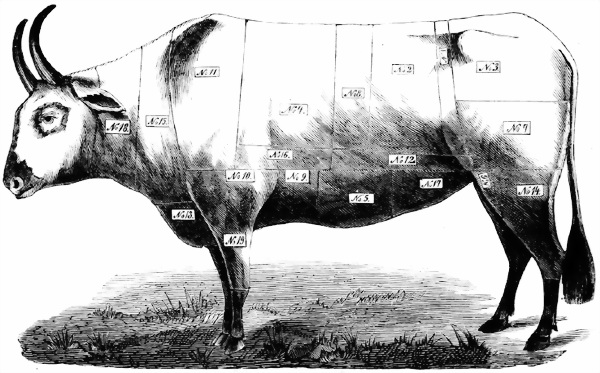
\includegraphics[width=\textwidth]{01.jpg}

Фигура 1-я изображает целого черкасского быка в натуральном его виде, а нумерованные подразделения означают места, где находится каждый из вышеупомянутых кусков.

Вот объяснение этой номенклатуры:

\noindent1. Английский филей. \\ 2. Толстый филей или вырезной. \\ 3. Огузок. \\ 4. Тонкий край. \\ 5. Завиток. \\ 6. Кострецы или подпашки. \\ 7. Середина бедра. \\ 8. Тонкий филей. \\ 9. Середина грудины. \\ 10. Середина лопатки. \\ 11. Толстый край. \\ 12. Подпашек \\ 13. Чолышко. \\ 14. Подбедерок. \\ 15. Оковалок. \\ 16. От края покромки. \\ 17. Бочок. \\ 18. Шея или зарез. \\ 19. Рулька.

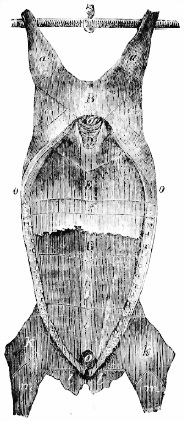
\includegraphics{02.jpg}

Фиг. 2-я есть туша, уже очищенная и развешенная на железных крючьях, при помощи палки, которую мясник продевает сквозь голяшки задних ног.

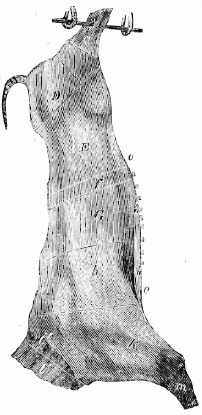
\includegraphics{03.jpg}

Фиг. 3-я есть та же туша, изображенная только боком, для большей ясности описания ее отдельных частей.

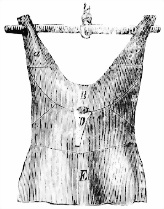
\includegraphics{04.jpg}

Фиг. 4-я представляет заднюю часть туши со стороны хребта.

Во всех этих фигурах одинаковые буквы показывают одни и те же куски туши, так что, рассматривая их в трех положениях, можно отлично заучить их отдельные формы.

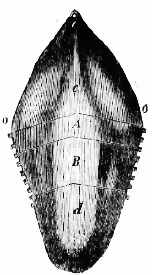
\includegraphics{05.jpg}

Фиг. 5-я изображает грудину с лицевой стороны.

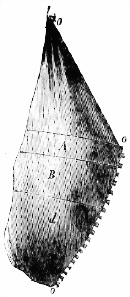
\includegraphics{06.jpg}

Фиг. 6-я изображает ее же сбоку, и здесь одинаковые буквы снова указывают на одинаковые куски или отдельные части грудины.

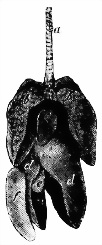
\includegraphics{07.jpg}

Фиг. 7-я изображает внутренности быка, т.~е. сердце, легкие, ливер, дыхательное горло, печенку и желчь.

Рассмотрев каждую фигуру по различным ее буквам, мы вполне и безошибочно ознакомимся со всеми частями туши.

Фиг. 2-я, 3-я и 4-я.

B. Нижняя подбрюшная часть или ссек, употребляемый преимущественно на жаркое,

а. а. Два подбедерка, идущие для бульона, если желаете иметь его наварнее.

C. C. Два подпашка, имеющие назначением заготовляться в прок в виде солонины.

D. Огузок, лучшая часть из всей туши, доставляющая отличный бульон; но и подаваемая отдельно в виде разварной говядины, или даже жаркого.

а. Часть дыхательного горла.

bb. Легкие, окружающие сердце; их употребляют в рубленом виде для пирогов, а иногда делают вкусное блюдо, называемое гаши (gachi).

с. Самое сердце.

dd. Гусак, или ливер; идет в начинку пирогов.

е. Печенка, из которой приготовляют род котлет.

ff. Желчный пузырь, материал для составления красок, а также употребляемый во множестве в аптеках.

Для лучшего узнавания этих отдельных частей бычачьей внутренности мы укажем и на различные их колера, как напр. сердце имеет темно-вишневый цвет и величиною бывает до 7 вершков, легкие~--- это мясистый, розово-фиолетовый кусок, гусак и печенка темно-вишневого цвета и две почки~--- тёмно-красные, глянцевитые куски мяса, облитые очень вкусным жиром. Почки употребляются под соусами и в суп-рассольник, а сало, их окружающее, идет во многие пирожные и в особенности в пудинги.

E. Филей, лакомая, по своей мягкости и сочности, часть туши. Филей разделяется на два сорта: английский и внутренний или вырезной. Места, ими занимаемые, указаны на фиг. 1 под №№ 1 и 2. Английский есть задняя часть филея, и его всегда почти употребляют на ростбиф, а вырезной доставляет настоящий бифстекс. Иные хозяйки берут филей для бульона, прельщаясь его мягким мясом в разварном виде; но это плохой расчет: филей стоит дорого, весу имеет очень много, потому что в нем заключается большая кость, а бульон от него никогда не бывает достаточно крепок, так как кость эта не имеет мозга.

F. Тонкий край, или I ребро, отсеченное в толщину всей туши. Из этого куска изготовляются котлеты, отделив мясо от костей, и его же употребляют на душеную говядину, так как вырезка его мягка, мясиста, хотя гораздо тверже филейной вырезки. Пользуясь неопытностью своих молодых хозяек, кухарки нередко заменяют этой вырезкой настоящую филейную и ставят ее на счет по той же дорогой цене. Филейная вырезка шире, мясистее и окружена большим количеством жира.

G. Грудина, т.~е. следующие за первым ребром четыре ребра, отрубаемые все вместе, чтоб составить этот кусок, употребляемый преимущественно для говяжьего битка.

H. Толстый край или оковалок, заключающий пять ребер и употребляемый для жирных щей.

I. Шея покупается для навара.

К. К. Две лопатки, идущие в развар для бульона.

М. М. Две голяшки, т.~е. оконечности передних ног; они жилисты, но дают превосходный, студенистый бульон, очень полезный для слабых людей; только должно старательнее снимать пену и давать долго кипеть: иначе бульон будет мутен и приобретет какой-то посторонний неприятный вкус.

L. L. Зарез, т.~е. самая оконечная часть шеи, жилистая, но годная для бульона.

оnо, оnо~--- покромки от края,~--- накожная мясистая оболочка, снятая с грудины и оканчивающаяся по направлению ребер; также идет в развар для бульона.

Р. (см. фиг. 8) изображает средину бедра, которую очень выгодно брать для бульона, так как в ней есть мозговая кость, а с тем вместе и мясо довольно нежно.

оооо. Показывает то место, или скорее ту впадину в туше, где находится грудина, которая изображена отдельно на фиг. 5 и 6-й.

С. (см. фиг. 5-ю) показывает бочок, или отдельную, верхнюю часть грудины, употребляемую для щей или борща.

А. Завиток есть та часть грудины, которая прилегает к двум первым ребрам и равномерно идет во щи или в борщ.

B. Собственно грудина, чрезвычайно жирная и хрящеватая часть мяса, состоящая из четырех ребер, и ее преимущественно употребляют, когда желают варить вкусный борщ.

d. Чолышко, нижняя часть грудины, мягкое и вкусное мясо, которое подают в виде разварной говядины с хреном.

Фиг. 7-я изображает внутренность быка, употребляемую в пищу, только тут не указаны рубец и селезенка, которая обвивается одним концом вокруг рубца, т.~е. большего беловатого куска внутренности желудка, а другим, т.~е. верхом, она находится в тесной связи с гусаком, или ливером. Селезенка имеет вид продолговатого, пестрого ремня мяситого цвета, с красноватыми и темными пятнами. Ее не употребляют в пищу люди; но она составляет часть, так называемой, кошачьей говядины, продаваемой гусачниками и кошатниками.

Мы уже сказали, что главная цель этого руководства~--- научить экономии молодых, неопытных хозяек. Для соблюдение полной экономии особенно при ограниченных средствах, необходимо входить в самые мелочи, уметь распоряжаться провизиею так, чтобы ничего не пропадало даром. Само собою разумеется, что этого нельзя требовать от прислуги, а потому было бы крайне неблагоразумно предоставлять эти заботы повару или кухарке. Поясним все вышесказанное примером: хозяйка небольшой семьи, например, из четырех человек, при закупке провизии на неделю (само собою разумеется, зимою), купила следующее: 12 фунтов ссеку, заднюю часть телятины (фунтов в 8 или 10), две телячьи головы, судака фунтов в пять и полдюжины телячьих ножек. Этою провизиею она всего выгоднее распорядится следующим образом: распределит говядину так, чтобы кости и часть мякоти шли на четыре супа (см. ниже: отд. V. Навары, бульоны, супы и пр.), а лучший мякотный кусок на котлеты для одного дня, тушеную говядину для другого обеда и клопфлейш для третьего; на четвертый день можно поджарить ножки с полуголяшкой и подать их под каким-нибудь соусом, употребив отвар из них на суп (см. королевский суп); из судака можно приготовить уху, русскую, немецкую и проч., а его подать под белым соусом с каперсами, с яйцами и~т.~д. Из телячьих же голов можно приготовить студень или из одной сварить суп, прибавив к ней полголяшки (если хотят иметь крепкий бульон) и подать ее на второе кушанье под соусом. Из задней части телятины выйдет жаркое на один день, из остатков которого на другой день, прибавив какой-нибудь отварной говядины, можно приготовить рагу, а из отрубленной голяшки и брюшной части, как было сказано выше, суп. Таким образом, предположив, что подобная провизия закуплена в субботу, хозяйка может из нее приготовить следующие обеды:

Воскресенье: 1-й суп из говядины (мы сказали, что из ссека можно приготовить суп), телячье жаркое с огурцами и пирог или пудинг.

Понедельник: 2-й суп из говядины, студень из головы, рагу.

Вторник: Уха, судак под скоромным соусом с картофелем и, если желают, кисель, блины или каша.

Среда: Суп из телячьих ножек с голяшкой, ножки с фасолью, зеленым горошком и~т.~д.

Четверг: 3-й суп из говядины, тушеная говядина с картофелем.

Пятница: Суп (наприм. рассольник) из голяшки и брюшной части телятины; котлеты с чечевицей, горошком, пюре из картофеля.

Суббота: 4-й суп из говядины, клопфлейш, каша\footnote{Само собою разумеется, что эти примечания относятся только до людей с небольшими средствами, имеющих простой стол}.

К этому мы считаем не лишним присовокупить еще следующие замечания, которые, как ни кажутся маловажны, однако же, в общей массе и в особенности для людей небогатых, имеют неоспоримое значение. Замечания эти следующие:

Перья и пух с домашних птиц и дичи следует копить и, перебрав в свободное время, сохранять в сухом месте. Ими можно набить подушки, перинки для детей и проч.

Выгребать уголья из печки и из-под плиты для самоваров.

Если бьют дома мелкий скот, то кровь сохранять. Ее подливают, для удобрения почвы, под фруктовые деревья.

Телячьи рубцы, хорошо вымыв в нескольких водах, высушить. Они употребляются при изготовлении швейцарских и голландских сыров, как сычуги, или лаба, о чем подробности в статье: <<Молочня>>.

Шкуры с телят, баранов и проч., тотчас по снятии, растянуть на палочки, высушить и отдать для выделки кож.

При каждой кухне хорошо держать двух или более поросят, которых можно кормить помоями, остатками кореньев, хлеба и~т.~д.; нужно только остерегаться, чтоб им не попадало мяса и остатков дичи.

Мыло для стирки лучше всего закупать по несколько брусьев, смотря по величине хозяйства, и сохранять его в сухом и теплом месте, потому что сухое мыло тверже и спорче. На один пуд белья выдавать 1 1/4 фун. мыла.

Обязанность каждой, разумеется, провинциальной и даже, просто-напросто, деревенской, хозяйки~--- входить во все эти мелочные подробности, надсматривать за порядком и чистотой, и стараться, чтоб малейшая безделица не пропадала даром. В столицах и больших городах все это немыслимо.

В этом руководстве, при описании кушаньев, т.~е. в большей части всех поваренных рецептов, принадлежащих г-же Авдеевой, назначена пропорция на три человека, т.~е. такая пропорция, при которой за обедом из трех или четырех блюд может быть вполне сыто семейство из трех человек. Эту пропорцию можно увеличить и уменьшить по желанию; так, например, на шесть человек удвоить, на девять утроить, на два взять 2/3 и~т.~д. Вполне соглашаясь с практичностью такого замечание покойной г-жи Авдеевой и сознавая возможность производить все расчисления блюд по сделанным ею здесь указаниям,~--- мы, занимаясь чисто практическими прибавлениями к книге г-жи Авдеевой, признали еще вполне целесообразным дополнить полезные эти заметки совершенно особенным и взятым с самой сути дела подробным расчетом обедов в 2–3 блюда, готовимых не из запасов, а из покупаемой провизии ежедневно на 10 человек. Цифра эта чрезвычайно удобна, как единица для расчислений различных обедов: вдвое меньшего числа потребителей, или, напротив, вдвое, втрое, в полтора раза большего. Расчисления г-жи N****, имевшей любезность передать в полное наше распоряжение свои <<домашние записки>>, помещены нами почти в конце книги, при распределении обедов или, так называемых, <<обеденных записок>> (меню). Эти расчисления доведены до последней степени точности и аккуратности, что поставляет мало-мальски смышленую хозяйку в удобную для нее возможность по этим примерам высчитывать все блюда этой книги с большею верностью и правильностью, чем ежели бы хозяйка эта руководствовалась совершенно готовыми расчетами провизии на каждое блюдо, предлагаемыми крайне наобум некоторыми нашими новомодными поваренными книгами.

\section{БЕЗОШИБОЧНАЯ ПОКУПКА ВСЕХ СЪЕСТНЫХ ПРИПАСОВ ДЛЯ ЭКОНОМИЧЕСКОГО И С ТЕМ ВМЕСТЕ ХОРОШЕГО СЕМЕЙНОГО СТОЛА} % отдел 2

\subsection{Говядина.}
При покупке свежее бычачье мясо не трудно отличить от испортившегося\footnote{Указания и наставления эти, впервые являющиеся в русской домоводственной книге,~--- заимствованы из столичной петербургской торговли; но они могут быть легко применяемы к покупке съестных припасов и на провинциальных рынках.}. Хорошее свежее бычачье мясо отличается особым мясным запахом и ярко-красным цветом. Отрезанный кусок такого мяса имеет настоящий красный цвет и как бы мраморный твердый вид, причем прорез указывает на достаточное количество жира, находящегося между мясными волокнами. Самые волокна говядины должны быть нежны и сочны (обилие сока в мясе составляет существенное его достоинство). Вообще лучшее бычачье мясо доставляют волы, т.~е. кладеные быки. К этому следует прибавить, что не все части быка дают мясо одинакового достоинства: лучшие куски, которые и в торговле ценятся дороже, получаются из хвостовой и бедренной частей, из переднего ребра и~т.~д., что все подробно описано у нас здесь в сортах говядины, согласно с рисунками, на которых ясно и отчетливо обозначены все части (см. Отд. I). При этом следует также иметь в виду, что мясо старых и изнуренных животных вообще бывает жестко, сухо, маложирно; а мясо животных слишком молодых тоже не жирно и бледноватого цвета. Иногда продажное бычачье мясо, обыкновенно давно лежалое, смазывается свежею кровью, с целью скрыть от покупателя синевато-красный цвет такой говядины; но зоркий глаз покупателя может легко подметить этот обман по наружному виду такого прикрашенного мяса.

Известно, что самое лучшее бычачье мясо в петербургской мясной торговле есть черкасское. Это не подлежит никакому сомнению, хотя в последнее время, в эти годы, с 1871, в мясных лавках продавцы стали продавать много простой русской говядины от собственно русского скота из северных губерний. Но это последнее на вид светлее и имеет более волокон и менее осмазонных частей, почему его следует избегать для ростбифов, бифстексов и хороших бульонов. Впрочем, в торговле есть еще род мяса, довольно распространенный, который вкусом не хуже черкасского. но цветом гораздо бледнее,~--- это мясо, известное под названием яловицы. Оно получается от заяловевших холмогорских коров, хорошо кормленных, но негодных для дачи молока. Этого сорта говядины, повторяем, все-таки не дурной, в Петербурге развелось нынче не мало. Яловичное мясо хотя и бледнее, однако несравненно нежнее воловьего. к тому же и разрез каждой отдельной его части несколько меньшего размера против воловьего, например, <<вырезка>> из коровьего <<филея>> значительно менее вырезки воловьей, и поэтому куски бифстекса, само собою разумеется, будут миниатюрнее, хотя, повторяем, нежностью, мягкостью и пухлостью они превосходят бифстекс из самой лучшей черкасской темноцветной говядины, столь высоко ценимой любителями и поварами.

Когда хозяйка или ее кухарка покупает вырезку отдельно от общего куска филея, платя за нее, по нынешним (конца 1873 г.) ценам, от 40 до 60 к. за фунт, то она должна наблюдать, чтобы мясник выделял эту вырезку от ребер как только можно чище, при чем необходимо требовать, чтоб лишний жир был хорошенько срезан, оставляя только небольшое количество этого жира собственно для жаренья ломтей бифстекса в их природном соку. Из фунта хорошей, честно выданной продавцом, вырезки должно непременно выйти три порядочных куска бифстекса: но оконечная часть вырезки не может дать такого количества ломтей, потому что в этом месте вырезка суживается приметным образом.

Вообще, при покупке мяса хозяйка или ее кухарка должна, как говорится, держать ухо востро, не полагаясь на добросовестность мясника, сколько бы он ни уверял в своей честности. Да даже чем больше этих умасливательных уверений, тем хуже. Необходимо покупательнице зорко следить за положением весовых чашек, на которых взвешивается, большею частью с отменною ловкостью и быстротой, купленный, какой бы то ни было кусок мяса, причем не должно мясному продавцу позволять снимать с этих чашек этот кусок до тех пор, пока стрелка весов находится еще в колебательном состоянии, потому что именно это-то преждевременное снимание товара производит и создает те фантастические, мнимые осьмушки и полуосьмушки, которые в общем месячном итоге, при более или менее изрядном заборе мяса в лавке, составляют фунты, так непроизводительно, накладно отражающиеся в бюджете экономной и рачительной хозяйки. Кроме того, обратите ваше внимание на то, что мясные продавцы при вырубании некоторых частей, как, например, <<ссека>>, <<лопатки>> и <<края>>, умеют мастерски пользоваться неопытностью или невнимательностью своей покупательницы, употребляя хорошо известные им приемы, крайне невыгодные для покупательницы. Так, например, при отпуске 6 или 7 фунтов <<ссека>>, они отрубают всю кость, принадлежащую к этому куску, а, между тем, эта кость отдельно весит фунта два, так что, если отделить жир, сухие жилки и с толстого конца небольшую плоскую косточку, собственно мяса останется очень мало, что, само собою разумеется, вовсе не составляет расчета хозяйки, тем более, что в этой огромной, продолговатой кости заключается чрезвычайно мало мозга, так высоко и справедливо ценимого при варке бульона. Вот почему должно требовать, чтобы продавец мяса, вырубая кусок ссека в 6 или 7 фунт., разрубал кость как можно более вкось, оставляя у закупленного куска меньшую часть ее, и даже отделял бы сухую жилу. Этим настоятельным требованием хозяйка выгадает наверно фунт чистого мяса.

Покупая для щей или борща несколько фунтов краю, должно настоятельно требовать, чтобы мясник отрубал от ребер их обнаженные тонкие оконечности, так как они составляют вес, не принося ни малейшей пользы.

Но вот лопатка,~--- это именно тот сорт говядины, на котором преимущественно выигрывают мясники и теряют неопытные хозяйки. Сквозь лопатку, составляющую саму по себе кусок фунт. в 15, проходит кость, круглая, толстая, плоская и без всякого мозга сначала, но кость такая, которая далее превращается в прямую, выдолбленную, довольно длинную трубку, наполненную сочным мозгом, составляющим драгоценность бульона. Если покупательница желаете купить фунт. 5 лопатки, мясник норовит расположить свой кусок так, чтобы наставить нож сначала, т.~е. с толстого края кости, которую он перерубает и тогда очень обязательно отделяет долевой кусок мяса, ловко поворачивает его перед глазами покупательницы тою стороною, где был наставлен нож и где начинается пустота, которая далее составляет резервуар мозга. Разумеется, что крохотная толика этого костяного мозга появляется в углублении; но это количество так мало, а остальная часть кости так бесполезно тяжела, что в ущерб для кармана покупательницы набегает непременно фунт или полтора бесполезного веса. Вот почему должно требовать, чтоб мясник, оставив толстую, круглую кость в стороне, непременно вырубал бы из середины лопатки, и тогда обозначится сквозная, прямая, трубкообразная кость, в которой с обеих сторон будете виден беловато-розовый мозг. Приступая к варке бульона, эту кость отделяют от мяса, обвертывают кисеей, завязывают ниткой, чтобы при процессе кипячения мозг этот не вывалился из своего костяного ложа. Многие любят им лакомиться перед обедом, посыпая солью и закусывая хлебом.

\subsection{Телятина.}
Лучший теленок, для употребления в пищу, бывает шестинедельный или двухмесячный. Мясо его должно быть сочно и непременно белеть во время жаренья. Оно студенисто, сытно, равно полезно в пищу для людей всех организмов, хотя физиология доказывает, что оно заключает в себе питательных частей менее против бычьего мяса, т.~е. говядины.~--- Задней четверти теленка отдается преимущество; за ней следуют: часть почечная, т е. между кострецом и котлетами, котлеты, грудинка, лопатка, головка, мозги, ножки и печенка.

Телятина бывает в продаже двух сортов, т.~е. мясо телят, откормленных исключительно молоком~--- первый сорт и телят обыкновенных, кормленных без особенного тщания, но все-таки довольно жирных и мясистых~--- второй сорт.

Вес крупного откормленного теленка простирается до 6 пудов всей туши. В торговле существует довольно обыкновенный обман, состоящий в надувании цельного теленка для умножения его веса. Обман этот, впрочем, довольно легко узнается. Стоит только слегка прижать пальцем кожу у нижней части телячьей тушки: если кожа плотно натянута на естественном мясе, она не поддастся давлению, если же палец образует впадину, то значит, что теленок искусственно надут. Но главное достоинство теленка составляет белизна его мяса и жир, который должен закрывать толстым пластом во внутренности почки и внутренний филей. Иногда, и даже довольно часто, мясо теленка бывает недостаточно бело, а красновато чему причиною обыкновенно неудачный убой этого теленка, причем не было дано достаточно вытечь крови, а допустили ее разлиться по всему мясу и как бы напитать собою это мясо. Умелый мясник режет теленка с отменною быстротою, моментально перерезывая ему острым ножом в известном месте горло, и тогда кровь не разливается по мясу, которое бывает вполне бело. Еще случается покупать телятину с мясом жестковатым. Это происходит от того, что продавец продал телятину чересчур скоро после убоя животного, когда мясо еще <<не провяло>>, как говорится, и оказывается <<парным>>. Такую слишком <<парную>> телятину опытные хозяйки или обегают, или оставляют на несколько времени, т.~е. часов на 10–12, на леднике, ежели, конечно, имеют ледник, что в Петербурге в небольших хозяйствах, к сожалению, не есть дело обыкновенное.

Лучшая телятина привозится в Петербург с ноября месяца до весны.~--- Телята привозятся в Петербург из его окрестностей, в особенности из Новоладожского уезда, где есть целые волости, занимающиеся отпаиванием телят. Привозят телят также из Новгородской губернии, преимущественно из Тихвина, и из-под Выборга; но выборгские телята мелки и тощи, вообще плохи. Телята доставляются обыкновенно прасолами, которые скупают их по деревням в розницу у крестьян, везут партиями в Петербург и продают на площадке мясникам по несколько штук за раз, но не с весу, а на глаз и на ощупь.~--- Мясники бьют телят на <<шпарнях>> (бойнях в рынках, устраиваемых преимущественно в подвальных этажах под лавками), с платою по 10 к. со штуки за убой.

\subsection{Баранина.}
Баранина бывает русская и шлёнская. Первая пользуется значительным преимуществом перед второю, потому что она не имеет того неприятного, своеобразного запаха, которым снабжена последняя. Узнать русскую довольно трудно, и поневоле хозяйки должны доверяться добросовестности знакомого мясника, почему нельзя советовать покупать это мясо на Сенном рынке, напр. увлекаясь дешевизной. Впрочем, осязание может несколько руководить выбором баранины, потому что кожа шлёнского барана хотя и мягче, но как будто слегка намазана мылом, a русский баран имеет кожу грубее, суше, но жир у него белее и плотнее. Мясники также избегают показывать барана в шкуре,~--- равно как и теленка,~--- потому что шкура шлёнского барана имеет неприятный псиный запах.

\subsection{Солонина.}
Хорошая солонина имеет черно-красный цвет и все другие наружные признаки свежего мяса. Такая солонина должна сохраняться в бочонке, наполненном рассолом до краев. Солонина грязновато-белого цвета, не сочная, слишком мягкая и издающая неприятный запах, должна быть избегаема, тем более, что бывают такие случаи, что попортившаяся солонина оказывается ядовитой.

Вообще нельзя слишком советовать употреблять покупную солонину, тем более, что изготовление ее домашним способом вовсе не затруднительно, как это можно видеть из наших, здесь в этой книге в Отделе <<Кладовой>> предложенных рецептов, а солонина скороспелка, заимствованная нами из бывшего в 1861 году домоводственного журнала: <<Русская Хозяйка>>, есть истинно гастрономическое лакомство, доступное для всякого хозяйства.

\subsection{Свинина.}
Свинина, получаемая от хорошо выкормленных, не старых свиней, отличается белым цветом, нежностью и не слишком обильным, довольно умеренным, пропорциональным жиром, равно как весьма нежною кожею. Окорок, или копченая свинина, должен иметь в отрезе ломтя ярко-красный цвет; волокна мяса, при всей своей нежности, не должны разлезаться и разрываться, a непременно иметь компактность. Жир в дурном окороке обыкновенно бывает мягок и даже как бы мажется; волокна же мяса представляются в разрезе зеленовато-желтоватыми и грубыми. Следует быть очень осторожным при покупке различных колбас и мясных фаршей, так как все эти товары приготовляются, к сожалению, крайне небрежно, из разных мясных остатков, иногда значительно попортившихся. Преимущественно надо остерегаться, так называемых, <<кровяных>> и <<ливерных>> колбас. Долго лежалые и потому испорченные колбасы, как известно, даже ядовиты. Отличить такие колбасы не трудно, так как они мягки, как каша, местами окрашены ярко-красным цветом с зелеными и белыми прожилками. Когда желают узнать, не приготовлена ли колбаса из попорченного мяса, до покупки, с согласия продавца, обливают колбасный фарш водою, кипятят его и затем прибавляют в эту смесь известковой воды (ее всегда легко достать без рецепта в аптеке); если колбаса сделана была из попорченного мяса, то, при обливании помянутой смеси известковой водой, из нее выделится особый газ, по запаху сходный с тем, который выделяется из отхожих мест.~--- Впрочем, как ни положительно верно это средство, лучше обходиться без приложения его к делу, на какой конец необходимо должно брать все свиные продукты и различные из них приготовление в хороших колбасных лавках, приобретших заслуженную репутацию и громко известных в столице, где они привлекают глаз покупателя превосходными своими эталажами в витринах. К сожалению, все это немецкие фирмы; что же касается до наших любезных соотечественников, русских колбасников, то к ним обращаться невозможно с той же доверчивостью.

\subsection{Живность.}
Торговля <<живностью>>, т.~е. дворовой (домашней) птицей, вмещает в себе: кур, петухов, цыплят, самоклёвов, каплунов, пулярдок, индеек, колкунов, гусей, уток и, в весьма ограниченном количестве, домашних голубей, впрочем, самых молоденьких, употребляемых почти исключительно иностранцами, всего больше французами. Оттого в куриной торговле, или в торговле живностью, ввелось и самое название этой птицы, переделанное с французского языка: пижоноты (pиgeonneau), т.~е. молоденький голубь.

Поименованная здесь птица всех наименований идет в продаже как живая, т.~е. покупаемая живою и убиваемая продавцом, большею частью, в присутствии покупательницы, или так, преимущественно, в битом виде, т.~е. так называемая <<битая>>, сохраняемая в ледниках. Такая птица, сохраняемая в превосходных кладовых куриного ряда Мариинского рынка (бывшая Щукина двора), в Чернышевом переулке, представляет собою удивительный консерв, похожий твердостью на мрамор, и купленную там именно такую замороженную, закристаллизированную живность можно употреблять совершенно безопасно: когда она у вас в кухне оттает, то, конечно, никто не отличит ее мяса от мяса только что сейчас заколотой птицы. Но, однако далеко не во всяком леднике, не имеющем специального применения для сохранения живности, может быть сохраняема с успешными вполне результатами битая птица. В дурном леднике мясо птицы принимает тот затхлый вкус, который обегают истинно сведущие покупательницы, не допускающие в хозяйстве своем никакой провизии с мало-мальским несвойственным ей запахом. Впрочем, вкус и запах эти только не страшны кухмистерской кухне, богатой искусственными, почти химическими, средствами для окрашивания, маскирования вида и изменения вкуса съестного товара.~--- Замороженные в течение зимы в мариинских погребах консервы всякой, разумеется, стоящей такого сохранения, живности могут вполне состязаться с самой свежей живностью.

К числу обманов в торговле живностью принадлежит <<надуванье>>, которое и составляет настоящее <<надувательство>>. Дело в том, что мелочник-продавец, преимущественно торгующий не в лавке, а в разнос или на Сенной,~--- этом обширном поле всяких фокусов съестной торговли,~--- купив тощую птицу, старается пустить ее в продажу <<хазовым концом>>, а для этого надувает эту птицу, т.~е. вводит внутрь нее, чрез заднее отверстие, воздух, и зашивает отверстие с некоторым искусством и маленьким фокусничеством. Таким образом, надув продаваемый предмет, назначенный в продажу малоопытному покупателю, <<надуваете>> и своего клиента~--- потребителя, который, по возвращены домой, при первых поваренных приемах, уразумевает, что им не очень-то дешево заплачены деньги за костяк. В таком виде купленная им птица к столу, мало-мальски порядочному, в виде фрикасе, жаркого или в паштете, не подается, а употребляется не иначе, как на бульон для супов, на кнели и разного рода фарши.

Со всем тем весьма многие хозяйки, а кухарки сплошь и рядом, покупают у недобросовестных продавцов дешевенькую надутую птицу, которая, чрез эту самую манипуляцию, может повредиться скорее и легче птицы, не подвергнутой вкачиванию в нее воздуха, способствующая, правда, ее округлению, но не защищающая мяса от зловредных последствий. Между тем те же неопытные покупательницы обегают ту продажную живность, которая, будучи тщательно выпотрошена от всех ее внутренностей и желудочных нечистот, имеет в пустом пространстве, образовавшемся от отсутствия внутренностей и всех потрохов, некоторое количество чистой пакли, весьма простосердечно и откровенно вводимой продавцом чрез гузку. Предрассудок, что всякая птица, набитая этим посторонним веществом, представляет собою снедь не только не вкусную, но вредную для здоровья, положительно не имеет никакого основания. Практика и продолжительная наблюдательность, опирающиеся на исследованиях точных и научных, убеждают в том, что без этой пакли, перед приготовлением птицы тщательно, разумеется, из нее вынимаемой, живность могла бы подвергнуться скорее порче и разложению, от которого именно этою самою паклей она защищена. Не говорим уже о том, что форма ее от этого делается красивее и представительнее. Впрочем, добросовестные и непричастные никакому шарлатанству торговцы обыкновенно именно так объясняют, даже это обстоятельство своим малоопытным покупательницам.

В летнюю пору в Петербурге парная живность, т.~е. только что заколотая, дорога и редка. И вот, в эту-то пору, ежели кто желает

\subsection{Дичина.}

ным. Между тем надо вам знать, что существуют дешевые сорта дикой птицы, которую можно с большим успехом накрывать силками и добывать другими способами, отнюдь не тратя на нее заряда, обходящегося выше той ценности, за какую можно птицу эту продать. Однако, смело можем уверить вас, ни одна из этих птиц, которые не убиты дробью,~--- не задавлена, так как, поверьте, задавливание могло бы совершенно испортить цвет и вид и нарушить вкус птичьего мяса, почему изловленных за раз, большею частью, в порядочном количестве, птиц убивают обыкновенно очень быстро, палкой, не подвергая их ни малейшим мучениям, могущим, повторяем, вредно отозваться на самое достоинство товара.

Рябчики,~--- это та дичь, которая в наибольшем употреблении повсеместна. Рябчики по цене своей, всего доступнее с осени до февраля месяца, хотя в курятных лавках Мариинского рынка, особенно, у известного поставщика Высочайшего Двора Никиты Федоровича Кузьмина, можно иметь, конечно за высшую цену, во все лето превосходно сохраненных во льду рябчиков. Однако недобросовестные продавцы выдумали фокус, как обманывать неопытных хозяюшек, продавая им за рябчиков, даже летом, птичку совершенно ощипанную, без перышков, которая есть ни что иное, как молоденькие, еще не умеющие летать, домашние голуби, плодящиеся в таких огромных количествах на чердаках наших столичных рынков, где на них, по найму лавочников, безжалостно охотятся уличные мальчишки, и преимущественно трубочистные ученики, великие мастера лазить по крышам. Цвет и характеристика мяса этих <<фальшивых>> рябчиков, ни дать, ни взять, как у настоящих. Обман обнаруживается при жареньи. Еще часто торговцы продают рябчиков слишком молодых, имеющих чересчур мало мясистых частей. Такой рябчик-цыпленок от совершеннолетнего рябчика, особенно, отличается тем, что у него ножки почти голенькие или мало опушенные мелким перышком. Между тем, чем старше птица, тем ножка больше обута, что называется в птичной торговле <<птица в сапогах>>. Лучшим рябчиком считается архангельский, появляющийся в Петербурге с ноября месяца. Хороши, впрочем, еще вологодские и сибирские. Из архангельских рябчиков советуем спрашивать у добросовестных торговцев тех, которые известны под названием колгачинских, отличающихся крупным ростом и необыкновенно сочным и вкусным мясом. Самыми плохими рябчиками считаются вельские, из Вологодской губернии: они всех других и мельче, и малосочнее. Еще превосходный сорт чердынских рябчиков из Пермской губернии, питающихся почти исключительно кедровыми орехами и потому называемых кедровиками. Эти рябчики выдерживают лежку долее всех других.

Дрозды дают жаркое посредственное, ни в каком случае не могущее идти на ряду с рябчиковым жарким; но под соусом бывают не дурны, и иным любителям очень по вкусу. Они <<парные>>, свежие, бывают в Петербурге только исключительно в октябре месяце. Во всю зиму можно дроздов иметь замороженных. Дрозд в особенности любит рябину, и этою ягодой почти одной питается. Если многоурожайна рябина, то и дрозда много; а как поест он всю рябину, то и отлетает дальше, где надеется на большее прокормление. Дрозда положительно никогда не стреляют, а накрывают силками и бьют палками.

Куропаток две особи. Это куропатка белая и куропатка серая. Вторая, т.~е. серая, достоинствами своими выше первой, т.~е. белой. Лучшая серая куропатка называется в лавках дончиха, т.~е. получаемая с Дона. Серая куропатка питается исключительно зерновым хлебом, предпочитая пшеницу всем другим сортам; белая же ест лесные ягоды и древесные почки. Куропаток продавцы продают со всею тою пищей, какая у птицы в зобу находилась в момент ее лова силками. Белая куропатка крупнее серой и показывается в Петербурге с 15 июля.

Тетерки и тетерева~--- птица полевая, питающаяся хлебом. Самая лучшая тетерка и тетерев сибирские, замороженные, появляющееся с половины ноября. Тетерев ростом побольше тетерки, но уступает ей вкусом. Весною тетерки~--- редкость, и в эту пору в торговле они называются орсезонами, как вероятно их прозвали французы-повара от своего слова hors-saison, т.~е. вне времени года.

Перепелка в Петербурге не в большом ходу и дорога. Лучший сорт называется курчанками, хотя получаются они не из одной Курской, а из всех смежных с ней губерний.

Глухарь и глухарка~--- не элегантное, но выгодное жаркое. Глухарка буро-серая, а глухарь синевато-черный; глухарь больше, даже гораздо больше глухарки, но мясо его грубее. Из одного глухаря выходите 8~--- 10 порций. Чем глухарь моложе, тем мясо его сочнее и приятнее.

Дикий гусь в петербургской торговле не в большом ходу и почете. Есть из них красноклювы и черноклювы. Последние известны под названием козарок и считаются вкуснее обыкновенных.

Дикая утка подразделяется на несколько сортов, по крайней мере на шесть, а именно: 1) кряква, 2) чирок (самые лучшие, самые крупные и мясистые), 3) шилохвост, 4) свиряга, 5) гогель и 6) сулок,~--- это уж сорта поплоше, и из них поплоше всех последний, т.~е. <<сулок>>, которого, однако, в продаже всего более. Мясо этого сорта дикой утки сильно отзывается рыбою, которою птица эта очень любит лакомиться. <<Чирков>> и <<крякв>> в Петербурге очень мало. Все эти птицы идут сюда наиболее с Ладожского озера, по осени.

Дупеля, бекасы и вальдшнепы носят общее название красной птицы, экземпляры которых в торговле показываются с конца июля месяца. Сезон для этого рода птичек с 15 августа и часть зимы.

Фазаны~--- блюдо чисто аристократическое и в домашнем быту недоступное, хотя все-таки и вам, хозяйка-читательница наша, на всякий случай не мешает знать, что фазанов несколько сортов: с ноября месяца показываются иностранные, прусские и австрийские, из которых последние преимущественнее первых, как крупностью, так вкусом мяса и красивостью пера. С января и по март являются наши астраханские и кавказские фазаны, замороженные, правда, не всегда вполне благополучно, так как местности, из которых везут эту птицу, не отличаются морозами. Астраханским фазанам, величаемым в торговле <<персианцами>>, уступают во всем иностранные.

Маленькие птички~--- общее название разных сортов лесной птички, употребляемой на фаршировку паштетов преимущественно, а отчасти она жарится особо, конечно, с величайшею осторожностью, и подается любителям этого жаркого пирамидою на блюде. С блюда птичек этих каждый на тарелку свою берет 5, 6 штук, употребляя только вилку, а отнюдь не касаясь до них ножом, который считается при этом вовсе ненужным. Птички эти, будучи изжарены, так малы и так нежны, что их можно, да и должно, по законам гастрономии, есть не иначе, как целиком с ножками, от которых в кухне отнимаются только цепки или ходочки, причем, впрочем, отнимаются еще и шейки, и головки. <<Маленькие птички>> общим этим собирательным названием покрывают различные мелкие породы, как: щуров, свиристелей, снегирей и воробьев, тех самых воробьев, которых мы в таком множестве встречаем везде и повсюду.

Покончив с дичиной в пере, т.~е. с птицей, обратимся к дичине в шерсти, т.~е. к лесным и полевым четвероногим. Из них прежде всего должно поговорить о зайцах, доставляющих на весьма многие семейные и домашние столы довольно хорошее и очень питательное, недорогое жаркое.

Зайцы делятся в торговле на два сорта, резко один от другого отличающиеся, а именно: а) беляк,~--- простая русская, весьма обыкновенная порода, совершенно как снег белая с зимы и пепельно-серого цвета летом, и б) русак, получаемый из северо-западных наших губерний и имеющий рубашку постоянно, и летом, и зимою, буро-сероватую; роста он очень хорошего, даже крупного и не в пример крупнее <<беляка>>. Стрелянные зайцы предпочитаются капканным по той причине, что стрелянный ест еще траву, а капканный питается исключительно древесного корою. К тому же капканный беляк бывает часто отвратительно изранен, что не мало вредит достоинству его мяса.

Оленина с весьма недавнего времени стала входить и окончательно вошла в съедобный репертуар петербургской кухни. Оленьи филеи~--- задние, так как передние части вовсе не привозятся из Архангельской губернии, откуда оленина идет к нам в замороженном виде. Это оленье мясо, надобно вам сказать, берется не от старых, бывших уже в езде оленей, каких множество петербургские жители видят зимою на Неве, а от годовиков, которые хотя и не телята, но все-таки еще пе старики. Эти годовики оставили уже молоко и ели траву и сено. Оленина продается цельными этими филеями от 4–5 р. штука, а фунтами можно иметь фунт за 12, 10, даже 8 коп. Торговый фунт оленьего мяса представляет собою больше мясного материала, чем такой же фунт черкасской говядины. В оленине нет ни костей, ни жил, ни хрящей, ни волокон, а питательность и сочность весьма удовлетворительные. Мясо это режется <<словно хлеб», как выражаются те, которые в этом свойстве этого мяса хотят видеть его, кажущиеся им, недостатки. Другие же, напротив, по этому-то самому и ценят высоко оленину, как мясо, именно режущееся подобно хлебу, а потому самому и особенно сочное. Точно такого же характера и мясо лося или лосина, которая нынче начинает очень распространяться в Петербурге. В одном из известнейших петербургских ресторанов, под фирмою <<Мильбрет», кормящем ежедневно до 700 и более человек потребителей, жаркое из лосины~--- говорят сделалось весьма обыкновенным блюдом.

Закончим этот длинный перечень сортов дичины несколькими словами о дикой козе или серне, которая в маринованном виде начинает являться на некоторых, впрочем, более роскошных и не чисто русских столах, польских преимущественно. Вес всей этой лесной скотинки от 1 п. 30 ф. со всем, т.~е. тут все части, а не как оленины~--- одни задние филеи, и все эти части с шкуркой и внутренностями, требующими немедленного выпотрошение. Цены дикой козы бывают разные: от 12 до 6 рублей штука; в морозы и в начале зимы она дороже, а при наступлении оттепелей все дешевле и дешевле, так как сохранение этих тушек с их внутренностями затруднительно и хлопотливо, почему торговцы рады-радёшеньки поскорее спустить этот неудобный товар.

\subsection{Рыба.}
Большое число постов значительно увеличивает в России потребление рыбного мяса даже и в тех местностях, где вовсе нет лова рыбы. Само собою разумеется, что живую рыбу, к какой бы породе она ни принадлежала, следует предпочитать при покупке рыбе сонной, мороженой, соленой и, наконец, копченой. В особенности необходимо избегать сонной рыбы и преимущественно в летнее время, так как она очень скоро портится, и, кроме того, неизвестно, что служит приманкой во время лова такой рыбы. Это тем более важно, что иногда рыбу ловят посредством шариков, скатанных из куколя и хлеба,~--- а куколь отравляет рыбу, почему ее употребление и бывает вредно для здоровья человека.

Более всего из рыбы, покупаемой не живою, распространено употребление сельдей, покупаемых в особенности для стола прислуги и рабочих. Поэтому не лишним считаем сделать здесь некоторые указание, при покупке этого рода рыбы. Хорошая сельдь отличается широкою жирною спинкой; мясо ее белое и нежное. Напротив того, следует избегать сельдь, если у ней мясо красноватое, шкурка легко отдирается, а глазное яблоко коричневое. Все это~--- отрицательные признаки достоинства рыбы. Голландские сельди или, скорее, шотландские,~--- каких наиболее в продаже и большею частью они идут в торговле за первые, которых очень и очень мало находится на петербургском рыбном рынке,~--- считаются лучшими, вследствие тщательного их очищение и солки. Норвежская сельдь отличается не совсем приятным вкусом, зависящего от содержание этих сельдей в сосновых бочках. Наша беломорская сельдь стоить в торговле гораздо ниже шотландской, хотя по белизне, жирности и вкусу и не уступает последней; но, к сожалению, она много теряет от неправильной ее укупорки и от крайне небрежной солки, подвергающей ее преждевременной порче. Другая рыба, имеющая в хозяйстве многообразное назначение и из которой приготовляются кушанья и не для стола прислуги только,~--- это треска или штокфиш. При покупке ее надо наблюдать, чтобы покупаемая треска имела хороший, ровный, сероватый или красно-бурый цвет, была бы без пятен и не имела бы затхлого запаху. Треска, ловленная в конце осени и зимою и оставляемая в соли до марта и апреля, далеко не так вкусна и нежна, хотя и белее мясом, чем треска весеннего посола. Треска, привозимая в Архангельск и идущая оттуда в Петербург, от небрежного соление ее в ямах, с употреблением слабой и нечистой соли, в пересоле бывает жгучею, а в недосоле~--- кислою и даже горькою, с весьма ощутительным неприятным запахом.

Сравнительно более легкая порча рыбы, встречающейся в продаже, зависит от большего или меньшего содержания в ней жира. Таким образом, в торговле чаще всего можно встретить испорченными: семгу, осетрину, севрюгу, сома, щуку, угря и пр. Вид такой рыбы снаружи бывает дряблый, волокна теряют связь; будучи сварена, она не так-то легко режется, сколько как-бы мажется ножом. Главный признак испорченности сырой рыбы есть то, что кости ее отстают от мяса, если, распоров живот, раздвинуть рукой обе полости. Глаз у свежей рыбы должен быть выпукл и светел. Напротив того, белое мясо рыб долее противится порче, именно вследствие малого количества содержащаяся в нем жира. К таким рыбам можно отнести: сига, судака, окуня, ерша, карпа, форель, леща, свежую треску, стерлядь и пр. Кроме того не следует забывать и то обстоятельство, что рыба, подобно вообще домашним животным, также подвержена болезням, при чем мясо, напр. у белой рыбы, получает желтоватый цвет и неприятный, затхлый запах, становится трухляво и пр.; мясо же больной красной рыбы, как, например, лососины, кроме трухлявости и неприятного запаха, отличается еще черноватым оттенком. К этим нашим замечанием необходимо прибавить еще, что рыба соленая, в особенности осетрина и белуга, вероятно от плохой посолки, бывает иногда ядовита. Надо быть также чрезвычайно осторожным при покупке копченой рыбы, так-как ее коптят не редко в то время, когда она попортилась и не находит сбыта. Вообще следует избегать заплесневевшей, трухлявой и горьковатой копченой рыбы.

Икра. Что же касается икры, то вообще надо заметить, что свежепросольная икра скорее портится, чем паюсная, а потому покупать ее следует с большею осторожностью и избегать такой свежепросольной икры, которая мало-мальски не зерниста, а напротив струиста, тягуча, сколько-нибудь кисловата и у которой икряные зернышки потеряли свою правильную сферическую форму. Хорошая же паюсная икра (салфеточная) должна быть сочна, жирна; зернышки ее не должны слипаться между собою, и вообще кусок ее должен представлять собою плотную, вполне компактную черную массу видимых и рельефных зернышек; излом же этой массы, при отрезе ножом, должен проявлять легкую потливость и иметь темно-серый отлив.

\subsection{Яйца.}
Ежели в Петербурге хотят иметь <<без обмана>> яйца высшего сорта и вполне свежие, и добротные, то необходимо обращаться за ними или к знакомым и полной вашей доверенности достойным торговцам, преимущественно специалистам яичной торговли, не торгующим положительно уже ни чем иным, кроме яиц, и торгующим ими с давних лет. Одна из этих специальных фирм, громко известная в Петербурге, есть фирма всеми уважаемого Алексея Федоровича Баранова, имя которого, как знатока этого дела, известно даже за границей. Склад его на Фонтанке, у Обухова моста. Впрочем, замечательно, что почти все лучшие яичные склады находятся по обеим берегам Фонтанки, между Аничковым и Обуховым мостами. Кроме того, яйца высших качеств можно найти еще и также брать с полною доверенностью в тех нескольких больших и пользующихся известностью в городе складах молочных скопов, которые поименованы нами ниже в наших заметках о молоке и молочных скопах. Заплатить за хорошие яйца несколько подороже, экономнее, чем, купив яйца очень дешево, испортить лежалым или тронувшимся яйцом какое-нибудь дорого стоящее и многих трудов требующее блюдо. Тут повторяется русская поговорка: <<от копеечной свечки Москва сгорела>>, потому что иногда между десятком употребленных вами в тонкое блюдо, как омлет, сабайон, слоеное тесто и пр., попадет одно плохое яйцо, хотя и не дешево заплаченное, по неумению выбрать взятое,~--- и все пропало! Вот для этого-то, не вдаваясь нисколько в теорию яичной торговли,~--- что не наше дело,~--- скажем несколько практических слов о том, как следует, по всем правилам, при покупке яиц в сомнительных лавках действовать, и, по поводу всего этого, упомянем только о том, что в Петербург яичный товар доставляется с начала лета до осени водою, а с ранней весны, с февраля месяца, начинают являться на яичном рынке яйца, привозимые по железным дорогам. Первые сохраняются в яичных кладовых всю зиму; вторые, по мере привоза, идут в потребление и бывает дороже первых. С недавнего времени показались в Петербурге яйца, так называемые, краковки, ранее всех других новопривозных появляющиеся, именно с февраля месяца, и идущие сюда из Кракова, Царства Польского и северо-западных губерний. Яйца эти соединяют в себе почти все достоинства, требуемые от хорошего безукоризненного яйца.

Само собою разумеется, что при выборе яиц, когда вы их покупаете в месте, не гарантированном правом слепой доверенности,~--- должно быть крайне осторожным. Иногда яйцо весьма нецеремонно говорит, о своей негодности, разя обоняние дурным запахом. Этот сорт яиц, легко обходимый всеми покупательницами. имеющими сколько-нибудь нормальное обоняние, называется в торговле <<тумак». Другие яйца поражают своим бурым цветом и резкою невзрачностью скорлупы, покрытой зловещими темными пятнами, признаками лежалости,~--- это также никуда негодные, сухие и несвежие яйца под наименованием пятинника. Затем есть сорт повыше этих, сорт дешевенький,~--- это присушка; оно свежо, но несколько деревянисто и уже ни под каким видом не может идти в такие блюда, в которых высокие качества яиц составляют особенную прелесть. Однако яйцо это годно в заливных, винегрете и некоторых других неделикатных блюдах. Выше этого сорта ординарка, которая сплошь-и-рядом идет во всех кухнях, хотя всмятку или вообще без соединений с другими материалами не годится. Советуем держаться еще высшего сорта, именно головки, пользующейся общею известностью и составляющей постоянный спрос всех хозяек и их кухарок, из которых далеко не все умеют, по тяжести в руке, отличить <<головку>> от <<ординарки>>. Но верх совершенства между яичными сортами~--- это клечик, а из <<клечика>>, то еще выше~--- <<козловка>>. Яйца эти, хотя и не несомые петербургскими курами и не те, о которых выражаются продавцы: <<сейчас из-под курочки>>,~--- отличаются всеми качествами яиц самого высокого достоинства и употребляются всмятку, равно как в самые изысканные блюда. Они привозятся по железным дорогам ежедневно во все времена года из низовых хлебородных губерний.

Степень свежести и лежалости яйца, не имеющего дурного запаха, как <<тумак>>, ни пятен и ржавчины как <<пятинник>>, узнается различными приемами и способами. Свежее яйцо должно быть тяжеловесно, так что при погружении в воду оно немедленно тонет и идет ко дну. Напротив того, не вполне свежее яйцо, хотя и не испортившееся еще, но давно снесенное, долго пролежавшее в подвале, бывает, сравнительно, легче по весу и при погружении в воду бульбулькает и всплывает на ее поверхность. Кроме того, если смотреть свежее яйцо на свечку или против солнца, то можно заметить, что оно слабо просвечивает в средней своей части; при разбивании такого яйца, желток явственно отделяется от белка. Вполне свежие яйца имеют совершенную полноту яичной массы и не содержать в себе никаких пустот. При некоторой опытности и сноровке, многие домовитые хозяйки, повара и знающие свое дело основательно кухарки узнают свежесть яиц следующим оригинальным приемом: лизнув яйцо сперва с острого конца, а потом с тупого, замечают, если тупой конец покажется на ощупь языка теплее острого,~--- то яйцо добротно и свежее; если же температура оказывается одинаковою как с тупой, так и с острой стороны, то яйцо сомнительно. Еще, при поднесении яиц к огню, свежее тотчас вспотеет и рука, его держащая, ощутить некоторую влажность, обнаруживающуюся и на самой скорлупе; не вполне же свежее и вообще лежалое яйцо никогда этого пота не даст. В торговле встречаются кроме того яйца, сохраняемый от гниения в известковом растворе или известковом молоке. Такие яйца неохотно покупаются домовитыми и сведущими хозяйками, потому что белок их чрезвычайно жидок, водообразен, трудно сбивается в пену и отличается посторонним неприятным вкусом. Яйца эти распознавать не трудно по чрезвычайной, неестественной белизне их скорлупы, которая в натуральном и нормально~--- неиспорченном своем состоянии должна иметь чуть-чуть искрасна-желтоватый колер. Наконец, при выборе яиц надо иметь в виду еще то, что лучшие яйца те, у которых скорлупа тонка, как-бы прозрачна и которые не столько шарообразны, сколько остроконечны с обеих сторон.

\subsection{Молоко и молочные скопы.}
Из всех съестных припасов, молоко и все из него приготовление или молочные скопы подвергаются бесчисленному множеству различных обстоятельств, вредно действующих на их качества и в особенности на их свежесть, потому что, как молоко во всех его видах, так и молочные скопы сохраняются крайне затруднительно. Так известно, что молоко уже через 23 часа, по выделении его из коровьего вымени начинает слегка изменяться, на поверхности его собирается слой сливок и тому подобное. Такая быстрота изменение молока вполне достойна сожаление, тем более, что, с одной стороны, в домашнем хозяйстве есть множество случаев, когда необходимо иметь цельное молоко, а с другой~--- вследствие неуменья торговцев обращаться с молоком и сберегать его на более продолжительный срок~--- в продаже вовсе не легко, как может казаться с первого взгляда, найти совершенно свежее цельное молоко. На сколько трудно найти в продаже хорошее цельное и даже снятое молоко, на столько же трудно судить о том, в какой степени виноват торговец, да и виноват ли еще он, если иной раз молоко, находящееся в его лавке, или синевато, или водянисто, или слизисто и пр. Вообще молоко, завися в своих качествах всецело от натуры коровы и способа ее содержание, может иметь все эти недостатки совершенно без злого умысла со стороны продавца. Это последнее обстоятельство делает чрезвычайно затруднительным наглядное различие в продаже молока неподдельного от поддельного, тем более, что последнее приобретает от подделки ту же водяность, синеватость и слизистость~--- свойства, которыми обладает молоко, взятое от больной коровы Впрочем, молоко разведенное водою (грубый обман, слишком обыкновенный в рыночной как гуртовой, так и мелочной торговле и преимущественно практикуемый петербургскими лавочниками и подвижными или ходячими продавщицами, известными под общим названием <<<<охтянок>>) может быть тотчас же узнано, так-как такое молоко, разбавленное водою с целью увеличение его объема, имеет обыкновенно светло-синий оттенок и бывает синевато-прозрачно у краев сосуда. Оно так жидко, что капля его, положенная на ноготь, не остается выпуклою, как это бывает всегда с неподдельным молоком, а расплывается; кроме того, оно мало или совсем не пенится и не пристает к чистому железному пруту если погрузить последний в молоко. Молоко, разводимое в торговле водою, бывает кроме того сгущено или мукою, или крахмалом, для того, чтобы скрыть что оно было разжижено водой. Если оно сгущено таким образом, то делается слизистым, и при расплывании на ногте и на краях сосуда оставляет осадок и крупинки, примешанных к нему, муки или крахмала. Сверх того, легко догадаться, что в молоке разболтана мука, еще и потому, что последняя имеет свойство пригорать и иногда обнаруживается на дне сосуда в виде бурого осадка, при кипячении молока. Кроме наглядного узнавание присутствия воды в молоке, введенной в него с целью обмана, можно применить еще следующее средство: следует влить определенное по весу количество (напр. 5–6 лотов) испытуемого молока в жестяную чашку, вес которой также предварительно определен. Затем прибавляют к молоку 30 лотов истолченного кварца, который всасывает в себя это последнее, образуя вместе с ним однородный сырой порошок, потом высушиваемый досуха и взвешиваемый; потеря в его весе, которая при этом обнаружится будет соответствовать количеству воды, содержавшейся в испытуемом молоке. Но при этом, однако, нужно помнить, что всякое нормальное, неподдельное молоко, как бы оно хорошо ни было, содержит в себе от 80 до 88 процентов воды. При описанном опыте, только излишек против этого количества должен быть признан за примесь, сделанную с целью обмана. Иногда, для сбережения молока, кладут в него поташ. Подмесь эту открывают, приливая в испытуемое молоко какой-нибудь кислоты, отчего, в случае содержание в нем поташа, произойдете шипение.

В хороших, ничем не подмешанных, сливках точно такой же существует недостаток, как и в хорошем, неподдельном молоке и притом сливки также, как и молоко, чрезвычайно легко скисают. Хорошие густые сливки не должны свертываться при кипячении. Пенистая, пузыристая поверхность сливок может служить наружным признаком, свидетельствующим, что они были предварительно разбавлены водой, а за тем и сгущены мукой и куриным яйцом. Для открытия в сливках присутствия муки, может быть употребляем тот же способ, который предложен выше для открытия этой примеси в молоке; примесь же яичного белка и желтка легко можно распознать по обильному образованию свернувшихся клочьев, получаемых после кипячения сливок и процеживание их через бумагу.

Творог вполне хорошего качества должен быть ярко-белого цвета, хрупок, отчасти слоистого сложение и сух. Если продажный творог сыр и студенист, то это может служить признаком, что он нарочно пропитан водою с целью увеличение его веса; творог же, имеющий зеленоватый оттенок, обнаруживает присутствие в нем сыворотки, которая, во время его приготовления, не хорошо была отжата.

Коровье масло совершенно чистое также не постоянно и не везде находится в торговле. Майское масло вкусом несравненно выше всех видов масла, приготовленных в другое время. Хорошее сметанное и сливочное масло должно быть однообразно во всей массе, нежно желтоватого, палевого цвета, на ощупь жирнисто, приятного, подобно орехам, вкуса и хорошо промыто; оно не должно, кроме того, нисколько хрустеть на зубах, от содержащейся в нем соли. Дурное масло, напротив того, бледного цвета, легко крошится, мало жирнисто и сухо, хрустит на зубах, пахнет горелым и кисло-горько на вкус; иногда же оно слизисто и тянется в нити. Масло часто бывает подкрашено нарочно, для придания ему привлекательного вида, в особенности в том случае, когда, как это с лавочным маслом сплошь и рядом бывает, к нему примешано сало, отчего оно делается слишком бледным. Разминая масло деревянною ложкою в воде, можно легко обнаружить, было ли масло окрашено или нет: если масло было окрашено, тогда и вода окрасится. Сало составляет самую обыкновенную и общеупотребительную торговую примесь в коровьем масле. Эту примесь можно открыть по вкусу и по виду такого масла: в разрезе оно имеет белые пятна и полосы. Гораздо реже встречается в масле, но все-таки встречается, примесь тертого вареного картофеля. Масло с этою примесью очень тяжеловесно, крошится, в разрезе шероховато; если растопить его, то на дне сосуда получатся мучнистые клочья, имеющие запах картофеля.

Топленое или русское масло редко встречается прогорклым и иногда бывает смешано с более или менее хорошим русским маслом и даже салом. Прогорклость русского масла, происходящая главнейшим образом от плохого топления, узнается на вкус; что же касается способа открытия смеси дурного масла с хорошим, то этот способ чрезвычайно прост: стоит только выложить такое масло из сосуда и сделать в куске разрез,~--- неоднородность массы легко обнаружит обман.

Все молочные продукты, не исключая и молока, в Петербурге продаются в различных лавках, вовсе не имеющих молочной специальности, или, в так называемых, весьма многочисленных, (более 1000) <<мелочных лавочках>>, с тою лишь разницею, что товар мелочной и, так сказать, <<энциклопедичной>> торговли в достоинствах уступает тому, который обращается в торговле более крупной и специальной. Так-то всеми молочными скопами торгуют, устроенные в домах и отчасти на рынках, сливочные лавки, где, однако, можно найти и яйца, и крупы, и макароны, и даже стеариновые свечи. С этими лавками соперничают <<зеленные лавки>>, держащие также: сливки, молоко, сметану, творог, масло и сыр простого, низкого сорта вместе с овощами, зеленью, соленьями, маринадами, копченою и соленою рыбою, живностью и дичью. Случайно и по давнишнему знакомству с хозяином лавки можно, конечно, и здесь в этих <<сливочных>> и <<зеленных>> лавках находить молочные скопы хорошего качества: но все-таки трудно, чтоб такой, например, нежный молочный товар, как сливочное масло или высшего сорта сливки могли находиться в соседстве с треской, балыком, чесночною колбасою и тому подобным без вреда для своего достоинства и качества, почему советуем хозяйкам за всеми этими припасами, ежели они желают иметь все такое, что хотя несколько и подороже, да уж затем представляет собою верх совершенства,~--- обращаться к специалистам торговли молочными скопами, которых, впрочем, очень немного, всего каких-нибудь шесть почтенных фирм, а именно: Максимов, Чернышев, Варламов, Сорокин, Татаринов (в Б. Конюшенной и в Б. Морской) и Ефимов, известный больше под именем Малиновского, по фамилии бывшего своего помещика, владевшего известною в окрестностях Петербурга мызою Суйдою, перешедшею впоследствии в управление и чуть ли не в собственность означенного г-на Ефимова. Торговля всех этих специальных лавок ведется в размерах широких, хотя, впрочем, и здесь можно иметь в самых малых количествах молочные произведение и цельное молоко самого высокого качества.~--- И так, положительный совет: стараться производить покупки по части молочных скопов или в этих больших и пользующихся весьма почтенною репутацией лавках, или в таких сливочных, добросовестность и дельность которых вам не с сегодняшнего дня известны. Впрочем, опытная и вполне знающая свое дело хозяйка, лишенная какими-нибудь обстоятельствами, например, отдаленностью своего местожительства, от центра города, где преимущественно находятся пункты торговли крупных специалистов, конечно, сумеет обойтись и без них, лично посещая <<свои>>, как говорится, <<насиженные>> места рыночной и лавочной торговли, где таких смышленых хозяек продавцы не надувают, оставляя арсенал своих торговых фортелей и фокусов для покупательниц менее сведущих и проницательных и в особенности для тех, которые учатся трудному делу домоводства и слишком доверчиво полагаются на своих кухарок.

Заведя речь о кухарках, кстати сказать, что все кухарки, особенно не немки и не шведки, a настоящие русские или отчасти и польки, и в особенности наиболее из них сведущие, необыкновенно пристрастны к употреблению русского масла, т.~е. топленого, которое, будучи копейками двумя на фунт дешевле обыкновенного чухонского кухонного масла, приготовленного из сметаны, но не топленого,~--- имеет отвратительное свойство страшнейшим образом чадить и дымить. Но на стороне достоинств этого сорта масла то, что оно не скоро портится, спорко для хранения и, как выражаются повара и кухарки, <<не капризно>>. Это выражение означает то, что при жарении с этим маслом, по свойствам его, нечего опасаться сжечь жаркое, которое можно оставлять довольно долго без присмотра на огне, а между тем уйти в лавочку, или в трактир, для различных каляканий и угощений. При употреблении же чухонского масла, этого рода вольностей дозволять себе нельзя, потому что как-раз жаркое подгорит. Впрочем, ежели вы жарите какую бы то ни было дичину, то, чтоб жаркое ваше достигало последней степени совершенства и имело золотистый цвет,~--- можно, с некоторыми предосторожностями от чада и угара, употреблять русское масло, точно так, как для жарения телятины оно нисколько не годится и непременно заменяется чухонским маслом или даже, что еще лучше, говяжьим почечным салом. И так, в маленьких, вполне опрятных хозяйствах, где и самые печи, и все очаги устроены ежели не роскошно, то удобно, комфортно, с правильною вентиляцией, и, главное, где глаз самой хозяйки за всем блюдет, там положительно и решительно можно сказать, что для всякого жарение другого кроме кухонного чухонского масла (которое под этим названием так и известно в торговле) употреблять не следует. Оно стоит, правда, от 30–35 к. ф., но не фарлатировано водою и даже салом, как дешевенькое в 20–25 к. ф., покупаемое у уличных разносчиков или у недобросовестных продавцов. И опять выходит дешевое на дорогое, потому что при промывке этого <<дешевенького>> масла, собственно масла в купленном фунте остается много-много две трети. Иногда, впрочем, масса воды в масле происходит от дурной его выпрессовки, чрез что оно рыхлится и увеличивается в объеме, что выгодно продавцу и убыточно покупателю. К тому же, дурно выпрессованное масло скорее портится и подвергается горьклости.~--- Лучшее кухонное масло коровье есть действительно, в полном значении слова, чухонское, потому что в громаднейших количествах доставляется из Финляндии, где на всех почти тамошних мызах выделка молочных скопов и в особенности масла <<кухонного>>, т.~е. низшего сорта, доведена до последней степени совершенства.

Независимо от кухонного масла, в торговле имеются другие сорта, а именно: мызное масло и сливочное масло. Первое очень хорошее, делаемое из сметаны и необыкновенно приятное на вкус, с легкой посолкой, идет в кухонном деле уже не на жаренье, а на более тонкие блюда, как яичные, овощные, хлебные (пюре, омлеты, пудинги, печенья и пр. и пр.). Этого же сорта масло особенно хорошо идет на домашние бутерброды. Но ежели хотят маслом лакомиться и употреблять его за обедом, завтраком, чаем, как это, по заграничному, ввелось у нас почти повсеместно, то уж тут необходимо иметь сливочное масло, доводимое ныне действительно до последней степени совершенства. Из этого сорта в Петербурге славится наиболее так называемое шварцовское масло, именуемое так по фамилии бывшего (в 1872 году умершего) владельца огромной мызы на границах Финляндии, где, как слышно, до 2000 дойных коров. Удобства сообщение дают возможность иметь в Петербурге все эти скопы и даже только-что подоенное молоко, по истечении лишь нескольких часов.

От масла перейдем к творогу. Не говоря ничего здесь о тех крайне неудовлетворительных и невзрачных сортах этого молочного скопа, какие обращаются в рыночной и низко-мелочной торговле, скажем, что те твороги, какие продаются в <<сливочных>> лавках, привозятся сюда с мыз, преимущественно ямбургских, гдовских и отчасти царскосельских. Они сохраняются на льду в погребах и могут быть получаемы покупателями во всякое время. Из этих же окрестных ферм доставляется и сметана. Узнавать достоинство сметаны и творога на вкус и на глаз так не трудно, что об этом и говорить нечего. А все-таки всего вернее покупать и то и другое в хороших лавках.

За сим скажем, что собственно молоко разделяется на два сорта: молоко снятое и молоко цельное. То и другое можно найти везде, но опять повторим, что ежели хотите иметь молоко самое чистое без всякого участия в нем воды, то все-таки надобно обращаться к фирмам почтенным, а не щеголяющим рыночными зазывами и всяческими шарлатанскими вывесками. В лучших сливочных лавках молоко и сливки получаются из ферм, расположенных по железным дорогам не более 100-верстного расстояние от столицы. Сливки подразделяются на три сорта: 1) низший сорт, т.~е. жидковатые, 2) средний сорт, т.~е. гуще, но еще не самые густые, и 3) высший сорт, т.~е. вполне густые, так называемые на сбивку. Все эти сорта сливок с порядочных ферм доставляются ежедневно в запломбированных бутылках. Владельцы лавок, так сказать, <<нанимают>> молочное хозяйство той или другой фермы, т.~е. по уговору с владельцем или арендатором фермы имеют определенное количество снятого или цельного молока, или сливок всех сортов. Запасаются они этим продуктом, большею частью, под наблюдением сведущего и добросовестного приказчика, постоянно находящегося на ферме от хозяина-нанимателя (т.~е. владельца лавки, производящей торговлю молочными скопами). Некоторые фермы, на ближайших дачах около Петербурга, имеют в столице своих агентов, которые в больших металлических, преимущественно цинковых, сосудах развозят молоко по домам своим месячным абонентам. При этом, они в этих же домах находят и других желающих снабжаться от них сливками и молоком. Сколько нам известно, этот способ продажи и покупки сливок и молока из первых почти рук не представляет собою больших неудобств для покупателя, при том, что продавцы, не платя ничего за содержание лавки, могут продавать молочный свой товар несколько дешевле сливочных лавок и магазинов; не часто бывают слышны жалобы на не добротность продукта, приобретенного таким способом. Однако, ежели кому нужны сливки действительно самого высокого качества, то знатоки дела советуют обращаться все-таки в магазины одной из шести выше названных нами фирм.

Парное молоко с некоторого времени в Петербурге можно иметь из тех городских ферм, которые в количестве, кажется, 50–60 рассеяны по Петербургу и содержатся большею частью отставными гвардейскими унтер-офицерами или мещанами, а больше всего разными вдовами~--- солдатками, мещанками, крестьянками, чиновницами, дворянками и пр. Фермы эти ни что иное, как 5~--- 6, много 10–12 коров молочных, содержимых, вопреки всем правилам молочного хозяйства, в темных и душных денниках и содержимых то и кормимых не всегда и не у всех хозяев с надлежащею тщательностью и, главное, опрятностью. Иногда удается получать от этих молочниц и молочников продукты недурные и порядочно приготовленные, как-то: молоко, сливки, сметану, творог, простоквашу, варенцы и пр.; но это случается не часто. Фермы эти или молочни с коровниками рассеяны чуть ли не по всему городу, и вы можете видеть множество на домах больших и малых (большею частью малых, в виде ярлыков об отдающихся квартирах) вывесок с надписями: <<Парное молоко. Цельное молоко. Снятое молоко. Сливки>> и пр. и пр.~--- Остается сожалеть, что это дело у нас хотя и развивается, но плохо как-то прививается. При этом, мы пройдем молчанием те крайне неудовлетворительные молочные заведение, какие устроены в наших общественных садах и скверах каким-то тирольцем, потому что в этих молочных с коровниками именно нет и в помине того, что составляет непременное условие всяких молочных скопов,~--- самой изысканной чистоплотности: здесь же, к сожалению,~--- отсутствие самой простой и необходимейшей опрятности, без которой никакое молочное хозяйство немыслимо.

Но пожелаем городским фермам успеха и развития несколько совершеннее того, какими они отличаются ныне,~--- и обратимся к, так называемому, русскому сыру, который в нынешнее время в весьма значительном количестве изготовляется в различных губерниях России и появляется большими массами в Петербурге, где не так давно еще славился и в общем употреблении был сыр, известный под названием мещерского, под каким именем, однако и поныне, по старой памяти, в продаже идут очень многие другие сыры. Этот <<русский>>, или туземного приготовление сыр, подражающий швейцарскому, голландскому, английскому и итальянскому сырам, преимущественно требуется для кухни и, отчасти, его сорта попроще во многих хозяйствах составляют хороший завтрак для прислуги. В настоящее время считаются хорошими сырами из сыроварен: артельных Тверской губернии (г. Верещагина), тверских: гг. Татищева и Кисловского; Вологодской, г. Денежкина, а также из многих мест Северо-Западного края. Между прочим, очень замечательна фирма братьев Кублей из Пошехонского уезда, Ярославской губернии. Фирма эта нынче делается очень и очень замечательною.~--- Кроме всех этих простых русских сыров из коровьего молока, употребляемых на кухне в различные кушанья, а в домашестве на завтраки запросто по домашнему, и особенно на стол прислуги, есть еще, так называемый, польский сыр. Сыр этот получается из Виленской губернии и, в своем роде, очень недурен. Он продается, смотря по остроте и спелости, от 15 до 60 к. за фунт. Попадается в торговле еще сыр из овечьего молока, получаемый также из Северо-Западного края и замечательный тем, что он имеет много сходства с пармезаном, почему довольно требуется знающими его такое свойство для макарон и вообще для блюд, заимствованных из итальянской кухни. Главное депо <<овечьего сыра>> в сливочной лавке в д. Семянникова, на Фонтанке, у самого Аничкова моста. Лавка эта содержится польскою уроженкой и отличается, приятною для глаз и обоняние, опрятностью.

\subsection{Овощи и зелень.}
В особенности весною все почти овощи, сохраняемые зимою с лета или с осени в подвалах, успевают прорости, при чем некоторые коренья, как напр. петрушка, сельдерей, морковь, свекла и другие овощи, каковы: картофель, брюква, репа и т. п., обращают свои соки на развитие и рост стеблей, листьев, корешков и корней, и в этом виде становятся совершенно негодными для употребления в пищу. Картофель же оказывается даже вредным, вследствие образования в нем в это время особая вещества~--- <<соланина>>, имеющего ядовитые свойства. Картофель, кроме того, бывает поражен этою болезнью, в последние годы очень сильно развивающеюся. В этом болезненном состоянии он отличается красно-бурыми пятнами, загнивает и в пищу оказывается негоден. Картофель с ростками бывает мягок, a после варки получает неприятный вкус; то же можно сказать и о тех родах овощей, которые к весне прорастают. К весне в особенности сильно изменяется капуста, сохраняемая в подвалах вилками в песке: наружные листья ее гниют и весь кочан издает очень резкий и неприятный запах. Подобная сильная порча овощей в весне происходить, большею частью, вследствие неуменья огородников сберегать их в зимнее время и от неимения на огородах хороших овощных амбаров. Во всяком случае, при покупке зимних овощей весною следует быть крайне осторожным и отнюдь не приобретать тех из них, которые обнаруживают признаки прорастание.

Все это нами сказано об овощах в натуральном виде, а не сушеных, квашеных, соленых и пр., почему надобно замолвить слово и обо всех заготовляемых в прок. Так, например, сушеный горошек, как простой, так и сахарный, имеющий в торговле несколько сортов, бывает очень часто перемешан с черным и серым горохом и другим сором; поэтому, при покупке его, необходимо обращать внимание на это обстоятельство, происходящее от плохой сортировки означенного товара. Вообще хороший горох должен быть чистого зеленая цвета (хорошо высушенный), без червоточины, и должен легко разбухать и хорошо развариваться в воде; закаленный горох трудно разбухает и разваривается. Все сказанное здесь о горохе может быть отнесено и к сушеной чечевице, при покупке которой необходимо, сверх того, обращать внимание на то, чтобы чечевичные зернышки не были сплюснуты, а имели бы свою натуральную форму и не были бы перемешаны с зернами куколя. При закупке кореньев в летнюю пору, надобно обращать внимание на их целость и на степень их сочности: чем сочнее корень редьки, моркови и пр., тем лучше; тогда нечего опасаться, что попадется корень стволовый, который, впрочем, можно очень легко распознавать по его сучковатости. При выборе квашеной капусты, необходимо обращать внимание на цвет, который должен быть светло-желтоватый; самая капуста не должна быть слизиста, горька и издавать того сильно неприятного, почти вонючая запаху, который так обыкновенен в наших торговых местах, где продается и сберегается этот продукт. Хорошие свежие огурцы, которые расходуются в таком множестве в Петербурге, не должны быть дряблы, желты и слишком крупны. Слишком крупные огурцы бывают или с большими пустотами внутри, или с сильно развившимися семенами. Хорошие же соленые огурцы не должны быть дряблы, желтоваты, едки на вкус и мягковаты; они должны сохранять в известной степени свой нормальный зеленый цвет, который иногда сообщается им искусственно посредством зеленого купороса, что очень и очень вредно. Эту фарлатацию легко заметить по зеленоватому оттенку огуречная рассола; нормальный же цвет этого рассола подобен цвету обыкновенного раствора поваренной соли в воде, с тем только различием, что огуречный рассол всегда бывает несколько мутный.

Впрочем, и относительно покупки овощей не могу не повторить вам того же, что уже говорено мною было, т.~е. что слишком дешевое все выходит всегда на очень изъянистое. А потому рекомендуем вам, петербургские хозяйки, как постоянные, так и временные, те две, три овощно-крупяные лавки, какие находятся на Екатерининской канаве, у Каменного моста, или, еще лучше, так называемое Коровинское овощное депо, принадлежащее первому по части огородных овощей специалисту A. Ф. Коровину, на Гороховой улице, у Красного моста, в доме Таля, на дворе. Здесь вы найдете все в совершенстве, в изобилии и, главное, здесь можно все брать с полнейшею доверенностью и уверенностью, что вас не обманут.

\subsection{Мука.}
Определение торгового достоинства муки затруднительно по той причине, что многие свойства и качества ее зависят сколько от честности торговца, столько же и от способа помола и условий роста того рода зернового хлеба, из которая она выделана. Так, например, несправедливо бы было обвинять торговца, если в муке, купленной из его лабаза, будет открыто присутствие, так называемых, рожков,~--- того самого ядовитого вещества, которое составляет болезнь ржи и пшеницы и смалывается вместе с зернами этих хлебов в тонкую муку, а будучи испечено в хлебе и потреблено человеком в пищу, производить в нем болезненные припадки, известные под именем <<злой корчи>>. Со всем тем, не смотря на чрезвычайную неустойчивость качеств муки, все-таки очень важно знать главные признаки хорошей муки. Таким образом, дознано, что хорошая пшеничная мука, почти единственная кроме гречневой для масляничных блинов и овсяной для некоторых похлебок, употребляемая в сколько-нибудь порядочных кухнях, должна быть однородна, т.~е. не различных сортов и помолов, на ощупь суха, мягка, пушиста, бархатиста и нежна. Тесто, из нее сделанное, должно иметь среднюю тягучесть: если тесто будет менее тягуче, то это будет служить признаком дурного качества этой муки. Плохая же мука, содержащая в себе много влажности (более 15 \% воды), обыкновенно легко приходить в брожение, съёживается в комья, имеет затхлый запах и дает худое, трудно поднимающееся тесто,~--- такая мука подверглась уже порче. Так-как сырость есть главнейшая причина порчи муки, то при покупке муки необходимо прежде всего обращать внимание на эту сырость, присутствие которой в муке обыкновенно узнается чрез то, что мука (все равно, пшеничная или ржаная) всегда имеет синеватый отлив, тогда как сухая мука имеет отлив желтый. Мука, попортившаяся от нагрева, что случается тогда, когда ее держат в помещении со спертым воздухом, при чем нижние мешки придавливаются верхними, отличается обыкновенно неприятным запахом и горьким вкусом. В пшеничной муке чаще всего можно найти примесь ржаной муки и картофельного крахмала. Для открытия этого обмана всего лучше взять пробу муки в лабазе, подвергнуть это количество муки брожению и испечь из нее булку: уже при 10 \% содержание в испытуемой муке означенного крахмала, вместо рыхлого и ноздреватого хлеба, получится твердая, неудобоваримая для желудка, лепешка. Что касается примеси ржаной муки, встречаемой в муке пшеничной, то она легко узнается по запаху и вкусу пшеничного хлеба, из пробы ее испеченного. Хорошая ржаная мука не так ярко-бела, как пшеничная, которая, лучшая, имеет положительно цвет первого снега. Самые высшие сорта ржаной муки, по белизне своей, подходят лишь к низшим сортам пшеничной муки; при растирании этой муки руками, она легко сваливается в комья, если даже и совершенно суха. Торговцы иногда обманывают покупателей, сбывая им низший сорт муки за высший; но этому горю можно будет помочь только тогда, когда покупатель лично ознакомится с различными торговыми сортами муки.

Впрочем, для всех печений в кухне и для всех хлебных блюд, в какие идет пшеничная мука, никакой другой этого рода муки употреблять не следует, как только ту, которая в торговле известна под названием конфетной. Она идет на пирожные, пироги, кулебяки, паштеты, клёцки, блинцы и прочие поваренные приготовление, имеющие мучное основание.

\subsection{Крупы.}
Крупы для кухни все должны быть самых лучших сортов. В избежание опасности купить сорт поплоше за сорт получше, можно хозяйкам, живущим в Петербурге, ежели они не имеют верной и вполне надежной знакомой <<зеленной>> лавки, посоветовать брать все сорта круп в тех немногих овощных лавках, которые находятся на Екатерининском канале, у Каменного моста. Здесь всего две, три фирмы, но весьма старинных и почтенных, действующих с полным уважением к своему делу, хотя, правда, у них всегда все немножко подороже; но мы уже остаемся при том мнении, основанном на опытности, что <<хорошее дорогое всегда выгоднее дешевой дряни>>. Однако, не все же могут для каждого фунта отправляться к Каменному мосту, да и к тому же, не у всех в квартирах есть порядочные кладовые (редкость в Петербурге) для делания запасов, почему волею-неволею, а приходится также покупать по мелочам и в разных, не всегда знакомых и не всегда вполне добросовестных лавках. И вот тут-то покупательница хозяйка или ее кухарка должна, например, при покупке перловой крупы предпочитать мелкую крупу более крупной, наблюдая, чтоб крупа эта была бела, без содержание крупяной пыли и мучнистых частей, зернышко к зернышку, как на подбор. Крупу пожелтевшую, или получившую серый цвет и затхлый запах, следует считать товаром более или менее испорченным. Эта крупа называется голландскою; она очень спорка и содержит в себе весьма мало мучной пыли, но все-таки ее следует перемывать. Простая, более крупная, сероватая и несколько продолговатая крупа, быв дешевле, употребляется в кушанья прислуги. Что же касается гречневой крупы, столь употребительной в русском хозяйстве преимущественно в виде каши, начинок (для пирогов и зразов), некоторых пудингов и для многого тому подобного, то в торговле существуют три главных ее сорта: а) ядрица представляет полное зерно не расколотой гречихи: лучшая ядрица должна быть тяжеловесна и в особенности суха; в ней не должно быть много черных или зеленых зерен или каких либо иных и сторонних примесей, например зерен сорных трав, что величайший ее недостаток. b) Так называемая продельная гречневая крупа есть второй сорт гречневой крупы. Зерна ее расколоты на две или на три части, следовательно, она мельче ядрицы. Этот сорт крупы должен быть особенно бел, сух и тяжеловесен. с) Третий сорт или ординарная гречневая крупа несколько крупнее предыдущего сорта и не столь бела, чиста и веска. Она известна также под названием казарменной гречневой крупы и, странное дело, любителями гречневой каши, сочной, упаристой, рассыпчатой, мягкой,~--- словом, настоящей <<русской каши>>, она предпочитается всем другим. Самый же высший сорт гречневой крупы из раздробленных круп называется в торговле вельегоркой и приготовляется исключительно в городе Моршанске; она гораздо мельче предыдущих сортов, совершенно чиста и не содержит в себе нисколько ни черных, ни зеленых зерен. Есть еще так называемая обварная гречневая крупа, продаваемая предпочтительно в зеленных лавках Каменного моста. Эта та же ядрица самого высокого достоинства, обданная самым сильным кипятком, просушенная и пущенная в продажу по 20 к. за фунт. Она красноватого цвета и изготовляется в горшке вдвое скорее сырой ядрицы. Наконец, так называемая смоленская, или манная крупа, из которой приготовляются все роды нежной молочной каши и, между прочим, знаменитая <<гурьевская каша>>, описанная в этой книге довольно подробно. Крупа эта очень мелкая; ежели она вполне хорошего качества, то не должна быть желтоватого цвета и содержать много мучнистых частиц. Прокислая манная крупа вовсе не годится в пищу.~--- Окончим сведение о крупах одною весьма употребительною в кухнях наших иноземною крупою, известною под названием сорочинского пшена, или риса. Хороший рис должен быть сух, бел, тверд, просвечивает, без обломков, не должен иметь неприятного запаха и кислого вкуса. Бразильский рис, известный в торговле под именем вест-индского риса и имеющий большие, белые, просвечивающие зерна, снабженные мелкими красными полосками, лучше итальянского риса. Но самый веский сорт товара в этом роде представляет каролинский рис: у него чистые, белые просвечивающие зерна, снабженные нежными полосками; он длиннее и более риса итальянского. Что касается русского риса (с Кавказа и из Крыма), то он, к сожалению, имеет посторонний неприятный вкус и запах и не редко содержит в себе примесь поваренной соли, которую примешивают к нему с целью сохранение его от червоточины. С некоторых пор в петербургской торговле появился новый сорт итальянского риса по 15 к. за фунт: зерна мелкие, голубовато-прозрачной белизны; он необыкновенно спорок и не легко превращается в кашу. Сорт этот превосходен для пилава.

\subsection{Фрукты.}
Из числа фруктов, по большому употреблению в кухонном хозяйстве, особенно замечательны лимоны. Тонкокожие лимоны самые сочные и дороже ценятся, но труднее сберегаются, чем толстокожие. Хороший лимон должен быть ярко-желтого цвета, без пятен; внутренность его должна быть с избытком наполнена соком свежим, приятно кислым, слегка липким и ароматным. Лимоны, у которых кожа покрыта плесенью, совершенно негодны. То же самое вообще можно сказать и об апельсинах, при выборе которых важную роль играет, как и при выборе лимонов, их тяжеловесность.~--- Яблоки и даже груши очень часто встречаются в совершенно гнилом состоянии на рынках, в особенности у самых мелких торговцев, к сожалению находящих себе покупателей, между тем как употребление таких плодов чрезвычайно вредно. Следует кроме того избегать плодов с повреждениями на коже и с пятнами. Хорошие финики, доходящие к нам уже в сушеном виде, должны быть полны, блестящи, без морщин и червоточины. Достоинство хороших винных ягод определяется их свежестью и сладостью; кроме того, они должны быть хорошо просушены, мясисты и без белого налета.~--- Изюм самый лучший считается тот, который называется пакетным. Но нельзя не предупредить доверчивых покупательниц, что эти <<пакеты>> заключают в себе много обманчивости, продаваясь от 1р. 50 к. до 2 р. за пакет в самых блестящих наших фруктовых лавках. Дело в том, что в пакете, в том виде, как он получается из Испании, вложена огромная изюмная ветка, восхищающая вас своею объемистостью; между тем такая ветка, при более тщательном ее осмотре, представляет собою связку из нескольких веток, которые будучи просто взяты из ящика, без помещения в замысловатый пакет, стоили бы не дороже 35–40 к. за фунт. Эту шутку играют испанские продавцы уже не с сегодняшнего дня, а мы все как-то ее не замечаем и идем добровольно на эту удочку.

Из сушеных фруктов в кухне большую роль играет чернослив. Лучшим черносливом считается французский и из этого французского выше других есть сорт, называемый <<империал>>. В фунте этого чернослива от 40–35 ягод, тогда как в других более простых сортах помещается в фунте больше ягод, а именно: в <<сюр-шуа>> (sur choix),~--- от 45–50 ягод; в <<шуа>> (choix) от 55–60 ягод; в <<рам>> (rame supérieure), самом обыкновенном, до 65 ягод. Ежели кто хочет купить в фруктовой лавке дорогой чернослив, не подвергая себя никакому обману или недоразумению, тот непременно должен обратить внимание на сообщенные нами здесь количества ягод в фунте, чтобы правильно и безошибочно судить о том, какой, наверное, сорт он покупает. Настоящий высшего качества бордосский или турский чернослив имеет прелестнейший аромат, долго не проходящий, когда откупоривается запаянная жестянка, в которой помещается эта изящная бакалея. В жестянках и банках сохраняемый чернослив остается без вреда для своей свежести неопределенное число лет.

\subsection{Грибы и шампиньоны.}
Главное условие при сборе грибов~--- уменье отличить съедобные грибы от ядовитых. Этим качеством не всегда бывают наделены лица, промышляющие грибами. Вот почему не редки случаи продажи на рынках ядовитых грибов вместе и с съедобными, так что покупатель должен быть непременно знатоком в деле выбора хороших грибов при их покупке. Можно посоветовать прежде всего покупать грибы не иначе, как на открытых, а не на потаенных или случайных местах; следует также избегать грибов крошеных и с очищенными корешками. Сверх того, необходимо иметь в виду и следующие соображение. Грибы, у которых мякоть не совсем свежа, или изрыта тонкими канальцами, доказывающими присутствие в них червей и т. п., не годятся для употребления. Иногда только одна нижняя часть гриба бывает источена червями, тогда как верхняя (шапочка) осталась неповрежденного. В таком случае верхнюю часть можно употреблять в пищу, а нижнюю следует отбрасывать. Наконец, хотя и взрослые грибы бывают годны в пищу,~--- также, как и молодые, однако все-таки лучше избегать употребление слишком уже старых грибов, отличающихся обыкновенно большими верхушками. К этому следует прибавить, что грибы, обрызганные сверху улитками, хороши и не опасны только в таком случае, если мякоть их не повреждена. При покупке соленых грибов, следует обращать внимание на рассол, в котором они сохраняются: если рассол тянется при переливании, а самые грибы покрыты слизью и издают плесневелый запах, или же горьки на вкус, то они не годятся для употребления.

Практическая заметка о шампиньонах.

Нынче употребление шампиньонов сделалось почти повсеместным; но грибы эти иногда и даже довольно часто оказываются ядовитыми. В сыром состоянии никак нельзя узнать ядовитости шампиньонов; но для того, чтобы удостовериться в их безвредности, необходимо брать их на пробу из знакомой лавки, или в лавке же, ежели согласится продавец, подвергнуть их следующему испытанию. Чтобы употреблять шампиньоны без опасения, режьте их пополам металлическим ножом и отнимите у них хвостики и лиственичные части. Ежели в этом состоянии шампиньоны сохранять свою белизну без изменения, по крайней мере, час,~--- вы их варите, оставив в кастрюле серебряную ложку. Ежели ложка или шампиньоны почернеют,~--- знак, что эти шампиньоны никуда не годятся и их надобно выбросить. Ежели же они цвета не переменяют, то их смело можно употреблять. Заметка эта, основанная на опыте, применима и к другим родам грибов\footnote{Заметка эта извлечена из статей бывшего придворного метр-д'отеля Эдмона Эмбера, печатанных в домоводственном журнале <<Эконом>> 1845 года.}.

\subsection{Сахар.}
В очищенных сахарных головах умышленных примесей не встречается; за то в сахаре, встречающемся в торговле, например, в виде сахарного песку, много бывает примеси в ущерб потребителям. Хороший рафинированный сахар в головах должен быть бел, отдельные кристаллы его должны быть правильны, однородны и блестящи. Такой сахар не должен быть мягок и в воде растворяться без остатка, без мути. Хороший колониальный сахар сырец бывает сух, цвета слабо-жолтого и состоит из крупных зерен. Иногда высший сорт сахара рафинад~--- содержит в себе, так называемый, некристаллический сахар, называемый виноградным, который притягивает влажность и таким образом нарушает связь между частичками сахара, отчего сахарные головы иногда распадаются в порошок. Для открытия присутствия означенного рода сахара, растирают немного испытуемого сахара с равным количеством гашеной извести; смесь эту растворяют в воде и раствор процеживают и нагревают: если он примет бурый цвет, то это будет служить признаком присутствия в испытуемом товаре некристаллического сахара.

Ко всему этому, относительно сахара, обращающегося в петербургской торговле, мы считаем не лишним прибавить, что сахар рафинированный на петербургских сахарных заводах в торговле петербургской называется <<петербургским заводским>>, в отличие от того исключительно свекловичного сахара, какой во множестве получается из Киевской и других юго-западных и отчасти Царства Польского губерний, который слывет под общим названием <<польского>>. Сахар петербургских заводов отличается замечательною крепостью и особенно сахар с завода фабриканта Кёнига, известный в столице, да и в провинциях отчасти, под названием <<кениговского>> или <<гранитного>>. Однако этот великолепный сахар уступает другим в сладости. К тому же, нельзя не заметить, что головы юго-западного или неправильно именуемого <<польского>> сахара крупнее голов петербургского заводского сахара. Не можем не обратить внимание на то, что в торговле существует, так называемый, <<постный>> сахар, при рафинировании которого употребляются на заводах точно те же далеко не постного, a вполне скоромного свойства вещества, какие употребляются и для рафинирования и непостного сахара; только та разница, что это сахар не сильно рафинированный, т.~е. не дошедший до степени кристаллизации, хотя нередко выходит из одной же с ним вари. Другой <<постный>> сахар, имеющий вид какой-то конфеты и иногда окрашиваемый в желтый или розовый цвета, продаваемый в фруктовых, зеленных и мелочных лавках, еще менее постного свойства, потому что просто-на-просто приготовляется пряничными мастерами на яичном белке.

Патока. Хорошо приготовленная крахмальная патока должна быть почти белого цвета, очень сладка на вкус, и погруженная в нее, для опыта, лакмусовая бумажка (ее легко достать во всякой аптеке) никогда не краснеет.

\subsection{Мед.}
Мед сотовый бывает слабо-желтого цвета, в свежем состоянии совершенно прозрачен, имеет приятную, цветочную душистость и сильно сладкий вкус. Плохой мед, получаемый чрез прессование сотов, при несколько возвышенной температуре, бывает бурого или красноватого цвета, мутен, не скоро превращается в зернистую массу, горьковат, кисел, содержит много воска и остатки пчел, легко приходить в брожение и пенится. Капля меду, в который подмешана вода, будучи опущена на тарелку, расплывается и тем обнаруживает обман. Мед, подмешанный крахмалом, при нагревании дает густую мутную массу, тогда как, будучи в чистом состоянии, он превращается при этом в совершенно прозрачную жидкость. Кроме того, вода не вполне растворяет такой мед.

\subsection{Уксус.}
Хороший, неподдельный уксус должен отличаться чистотой и прозрачностью; вкус его должен быть кислый, но не горьковатый, и тонкий запах его должен быть освежающий и приятный. Оставленный в покое, в хорошо закупоренном сосуде, он не должен даже по истечении нескольких недель давать осадка или делаться мутным. Самый лучший уксус есть винный (ренсковый). Он приготовляется из окисленного, чистого, прозрачного вина, чрез смешение его с уксусом и окисление такой смеси в больших бочках. Вкусом и ароматом он несколько напоминает то вино, которое было употреблено на его приготовление. Чем слабее уксус. т.~е. чем менее содержится в нем, так называемой, уксусной кислоты, тем легче появляются в нем серые студенистые клочья и развиваются в большом числе, так называемые, уксусные червячки. Вообще же признаки нечистого и поддельного уксуса обнаруживаются в малом содержании в нем уксусной кислоты, в темном его цвете, в остром вкусе, в значительном остатке при выпаривании его и пр. Для придание уксусу обманчивой крепости, иногда прибавляют к нему отвара или настоя каких-нибудь растительных веществ, имеющих остро-горький вкус, в особенности стручкового перца. Такой поддельный уксус производить в гортани и на языке жгучее ощущение и уже по одному этому признаку может быть легко отличен от действительно хорошего уксуса.

\subsection{Поваренная соль.}
Чистая поваренная соль должна быть белого цвета, тверда, чиста на взгляд и состоять из отдельных блестящих кубиков (тогда она не изменяется на воздухе), без запаха, солено-прохладительного вкуса, ни малейше не сера. Брошенная на раскаленные уголья, трещит от растрескивания кубиков и вследствие выделение находящейся в ней воды. Хорошая поваренная соль должна растворяться без малейшего остатка в трех частях холодной и горячей воды. Нечистота этой соли обнаруживается ее серым цветом, плохою кристаллизацией, расплыванием на воздухе, горьковатым вкусом, мутностью раствора, остатком, получаемым после выпаривания ее раствора на огне, и~т.~д. Между русскими сортами поваренной соли особенною чистотой отличается соликамская и дедюхинская, между немецкими~--- люнебургская. Большею частью недостатки нашей поваренной соли зависят у нас от небрежной ее промывки и просушки.

Заведя речь о поваренной соли, не лишне сказать, что в петербургском английском магазине и вообще во всех лучших наших фруктовых лавках продается столовая соль самого высшего качества, под названием ливерпульской соли, по 25 к. пакет (немного побольше фунта). Товар этот в продаже идет в синих бумажных пакетах с настоящим английским ярлыком. Никто не подозревает, что, покупая эту необычайно белую и нежную столовую соль, покупает такую соль, которая никогда в Англии не бывала, а есть настоящая русская соль, изготовляемая только особенным образом способами усовершенствованного рафинирование, известными некоему г-ну Соколовскому, владельцу той шоколадной фабрики на Лиговке, которая снабжает лотки с простонародными лакомствами тем шоколадом самого низкого сорта, который в таком огромном употреблении между нашими простолюдинами не только в Петербурге и Москве, но во всей России, хотя, правду сказать, шоколад Соколовского далеко не шоколад, a какие-то сахарные, и то из самого низкого сорта сахара, лепешки, чуть-чуть помазанные раствором жидкого шоколада.~--- Что касается до столовой ливерпульской соли, петербургского изготовление Соколовского, то остается сожалеть, что г. Соколовский, достигнув до такого высокого совершенства в приготовлении этого продукта, не заменит, наконец, заимствованный им иностранный ярлык русским, и не прекратит эту столь давнишнюю мистификацию публики, к сожалению, все еще падкой ко всему иностранному.

\subsection{Горчица.}
Ежели в сухом виде, то преимущественно покупается всеми, по справедливости, знаменитая <<сарептская>>. Ее можно иметь во всех бакалейных и фруктовых лавках, но в особенности с полною безопасностью можно ее приобретать в большой сарептской лавке в доме Сарептского общества, подле здание Почтамта, по Конногвардейскому переулку. В больших фруктовых лавках, равно как в магазинах Фохтса, можно с безопасностью покупать приготовленную жидкую горчицу, английскую и французскую; но надобно остерегаться от горчицы, так называемой, <<московской>>, состоящей из какой-то невозможной и непонятной амальгамы сомнительного свойства ингредиентов, продаваемой во многих <<зеленных>> лавках за французский товар, потому только, что для продажи этой дряни употребляются французские сосуды, украшенные нарочно выписанными из Парижа ярлыками знаменитой тамошней горчичной фабрики Maille.

\subsection{Оливковое масло.}
Оливковое масло, получаемое нами из южной Италии, уступает в доброте тому маслу, которое получается из Марсели и известно под названием прованского. В последние годы, благодаря удобству железных дорог, мы чрез Триест и Вену имеем этот товар и в зимнюю пору. К сожалению, однако, это оливковое масло, проходящее чрез руки триестских местных торговцев, всегда ими смешивается с семянным маслом, известным под названием <<сезамского>>. Чрез такую смесь или фарлатацию оливковое масло приобретает некоторую горечь, что далеко не принадлежит к числу совершенств оливкового масла, которое должно быть на вкус без всякого постороннего вкусового свойства, подобно чистой и хорошей воде, и таким-то образом оно узнается в своем достоинстве покупателем. Чистейшее прованское масло можно получать в фруктовом магазине г. Поэнта, в Апраксином дворе, именно потому, что владелец этого магазина находится в непосредственно прямых отношениех с марсельскими маслопроизводителями.

\subsection{Ваниль и корица.}
Ваниль в торговле двух отличительных сортов: мексиканская и бурбонская, т.~е. с острова Бурбона. Мексиканская ваниль имеет преимущество перед бордосской или бурбонской. В свежем виде оба сорта в качествах не различаются; но французская не выдерживает продолжительной лежки. Распределение стоимости ванили чрезвычайно многосложно: она зависит, во-первых, от степени длины палочки, доходящей от 4–8 дюймов; от цвета отдельных стручков, которые идут от темновато-рыжего до черного, как смоль; от степени зрелости, какая обнаруживается тем маленьким инеем (givre), род седины, который есть признак высшего качества ванили в глазах знатоков, принимаемый, однако за плесень невеждами, не смыслящими дела. Иней этот держится на ванили кратковременно, и исчезновение его умаляет ароматичность ванили, почему палочка ванили влажная, как-бы с потом, бывает достойнее той, которая потеряла свой иней или свою седину.~--- У нас в Петербурге в иных лавках, как русских, так и немецких, в особенности немецких, можно встретить ваниль из Гамбурга, замечательную своею дешевизною, выходящею на очень дорогое, потому что эта ваниль из Гамбурга есть ничто иное, как ванильная древесина, продаваемая услужливыми немцами-евреями петербургским доверчивым барыням-экономкам и оставившая свои соки в Германии на тамошних фабриках, изготовляющих эссенции и ароматические масла.

\subsection{Шоколад.}
Шоколад, как известно, делается из какао. В петербургской торговле 4 сорта какао, а именно: 1) Гуаяквиль, 2) Караказ, 3) Багие и 4) Тринитат. Самый распространенный сорт какао~--- это первый, Гуаяквиль. Это самый превосходный сорт, который советуем требовать в лавках, при покупке шоколада для особенно тонких кремов, пирожных, желеев и пр.; что же касается Караказа, который выше всех поименованных остальных трех сортов, то он светлее и нежнее их цветом, гуще и жирнее на вкус,~--- главное, имеет больше всех их питательных свойств, рекомендуется усиленно врачами выздоравливающим и вообще натурам слабым; но он страшно дорог и потому в шоколадную фабрикацию не употребляется. Ежели вы хотите купить для вашего стола или вообще для вашего употребление шоколада в чашках,~--- советуем спрашивать шоколад с этикетами известных фирм, каковы: в Москве Сиу, а в Петербурге: Ландрин, Виоле, Борман, Конради и Линуар.

\subsection{Миндаль.}
Миндальные орехи. под названием <<принцесские>> (amendes princesse) № 1 тонкокожие, a № 2 в соломке (à la dame). Орехи эти № 1 привозятся в бочках, a орехи № 2~--- в ящиках. Лучшие орехи французские, № 1, а похуже~--- португальские, № 2. Последние отличаются от французских миндальных орехов не столько тем, что крупны, сколько грубостью корки. Покупатель, увлекаясь величиною плода, не замечает толстой корки и покупает товар не высокого качества по довольно порядочной цене. Совет~--- не увлекаться величиною плода. Впрочем, самым лучшим привозным миндалем считается мессинский миндаль.

\subsection{Кофе.}
В петербургской торговле встречаются 6 сортов кофе, которые разделяются по чистоте запаха, крупности зерна и приятности вкуса таким образом: 1) Куба или кубский, 2) Цейлонский; 3) Порторико, 4) Ява или явский, 5) Лaгyaйpa и 6) Бразильский.~--- Истинные знатоки и любители кофе во всей Европе отдают преимущество <<явскому>> кофе; но в Петербурге, а потому и во всей России, он не столько, в ходу и в употреблении, как другие сорта, в особенности <<кубского>> и <<цейлонского>> кофеев. При этом, нельзя не заметить, что покупательницы кофе в особенности хлопочут иметь кофе очень круглый и очень мелкий, не подозревая, что слишком круглые кофеины~--- результат искусственного приема, потому что в фунте, например, плоского кофе непременно найдется несколько круглых зерен, оставшихся в нем по недосмотру того, кто занимается просейкою кофе на грохоте или сите. Это до крайности наивный фортель продавцов кофе, подметивших страстишку многих гоняться за круглым кофе, который в сущности ничем не лучше продолговатого.~--- Еще совет: не соблазняться, так называемыми мокским кофе или мока, какой, по более или менее доступной, но все-таки очень еще высокой цене, продается в фруктовых лавках в шикозных и красивых 20-ти-фунтовых плетушках. Истинного аравийского неподдельного <<мока>> в Петербурге бывает в год не более 250 пудов, стоимостью от 16–17 р. фунт, а весь этот аравийский и левантский кофе, каким мозолят глаза так беззастенчиво доверчивым покупателям наши коммерсанты-шарлатаны, есть ни что иное, как гамбургское изделие. В Гамбурге непочатый край всевозможных торговых фокусов и переделок, соперничающих с нашими шкловскими и бердичевскими метаморфозами. Такими образом, Гамбург дает Петербургу ежегодно до 1000 пудов своего <<мока>>, обморачивая петербуржцев, восхищающихся теми 20-ти-фунтовыми плетушками, очень, правда, щеголевато сделанными, в каких помещается гамбургский мока, состоящий из смеси подбора различных кофейных сортов. В этих сортах всегда можно найти некоторое количество зерен, схожих по наружному виду с настоящим мокским кофе, который, главное дело, отличается в неподдельном, как бы <<чистокровном>> своем виде чрезвычайною нечистотою укладки и отсутствием сортировки, тогда как этот исправляющий его должность <<мока>>, и продаваемый рублей за двенадцать 20-ти-фунтовая плетушка, отличается изящностью подбора зерна к зерну и аккуратнейшею, самою тщательною, чисто немецкою укладкой. Не нужно большой проницательности, чтобы видеть и понять обман.

\subsection{Саго.}
Особое крахмальное вещество, добываемое в Индии, Африке и Южной Америке из сердцевины некоторых видов тропических пальм, называемых саговыми пальмами, и известное в торговле под названием саго, бывает в чистом и натуральном своем виде белого, бурого и красного цвета. Зернышки его должны быть очень невелики, полупрозрачны, трудно раздавливаются между пальцами и трудно растираются в порошок без запаха и сладковатого слегка вкуса. Но этот товар довольно редок в торговле, а потому и дорог, не дешевле 25 коп. фунт.

Из русских фруктовых лавок можно найти это лекарственное снадобье, впрочем, употребляемое и в кухне на супы, пюре, пудинги и разные сладкие, весьма тонкие блюда, только у г. Елисеева, да еще у И. А. Поэнта, в Апраксином дворе, подле Коммисаровской школы; а то надо обращаться или к известной фирме бакалейно-аптекарских товаров Штоля и Шмидта, или в самые большие аптеки~--- Невскую и Аничковскую.

Обыкновенное же продажное саго, сбываемое в большинстве случаев за саго настоящее, состоит просто из крупинок картофельного крахмала, нарочно для этого приготовляемых по особому способу. Это картофельное саго, изготовляемое в огромных количествах в России на картофельно-мучных заводах, легко отличить от саго настоящего тем даже,~--- как бы ни было оно искусно подделано,~--- что оно удобно раздавливается между пальцами, что, будучи облито холодною водою, тотчас дает жидкость, немедленно окрашивающуюся от действия на нее иодной тинктуры (которую всегда беспрепятственно можно достать в аптеке) в синий цвет~--- признак, что исследуемый товар действительно содержит в себе картофельный крахмал,~--- и, наконец, что оно расплывается в горячей воде.

\section{УСТРОЙСТВО КУХНИ И ПОВАРЕННАЯ ПОСУДА} % отдел 3

\subsection{Устройство кухни.}
Кухни строятся различными манерами. Устройство кухни должно соответствовать достатку и образу жизни хозяина. Но как в среднем, так и в высшем сословиях, необходимо иметь в кухне русскую печь и английскую или немецкую плиту. Если состояние позволяет, то хозяйская кухня должна быть отдельна от людской, для соблюдения чистоты; здесь, кроме повара или кухарки, не должны толпиться другие служители. Русская печь необходима для печение разных родов хлеба, булок, кренделей и некоторых пирожных. Плиты делаются со шкафом и без шкафа. Плиту со шкафом называют английскою. Прежде были в большом употреблении очаги, но теперь их совсем оставили; только в больших кухнях очаги употребляются и до сих пор; они нужны для жаренья на вертеле жаркого. В небольших и средних хозяйствах легко можно обойтись и без вертела, имея в кухне русскую печь и небольшую плиту. Когда кухня одна для хозяев и служителей, в таком случае печь должна быть большая и устье у нее так высоко, чтоб можно было ставить в печь корчаги с квасом или пивом.

В кухне необходимы полки для посуды и шкаф, где класть разные припасы. В поварских кухнях делается каток, занимающий одну, а иногда и две стены; это род низкого шкафа; он, вместе с тем, служить и столом; внутри ого поделаны полки. Если он велик, то бывает разделен на несколько отделений, с особыми дверцами в каждом отделении. Столь есть вещь необходимая в кухне. Также не последнее удобство имеет в сенях кухни холодный чулан. В домах хорошо устроенных бывает недалеко от кухни погреб.

В кухне надобно соблюдать чистоту; посуда также должна быть вычищена, вымыта и расставлена по своим местам. Пыль со стен в кухне надобно обметать каждую неделю; полки наружный и в шкафах раз в неделю следует мыть щелоком с песком; стол или каток смывать всякий день. Пол, если он деревянный, должно мыть каждую в неделю и усыпать песком, а каменный — раз в месяц. Также надобно стараться истреблять в кухне мух и тараканов; для этого есть много безвредных средств, о которых будет сказано впоследствии.

\subsection{Поваренная посуда вообще.}
Кухонная посуда разделяется на деревянную, медную, железную и глиняную; здесь будет говориться о посуде, собственно принадлежащей к кухне. Из деревянной посуды необходимы: квашня для хлебов, и две или три поменьше, для булок, ситного хлеба и кренделей. В некоторых местах заменяют квашенки горшками или какой-нибудь другой посудой; но деревянные квашенки лучше, удобнее и прочнее. Лотки и ночвы для сеяния муки и вываливание теста для хлебов, булок и кренделей; доски, на которых рубят говядину, шинкуют коренья, кладут свалянные и приготовленные для печенья булки и крендели; разные веселки, мутовки и скалки; корытца и чашки, для рубления разных начинок, фаршей и тому подобного; лоханки для вымачивание мяса и рыбы; сита, разных сортов и решета. Все это можно иметь в большем и меньшем количестве, смотря по тому, сколько нужно. Но, чтобы для каждой хозяйки было виднее, то почитается нужным сделать полный реестр всей кухонной посуде, из которого можно убавить, смотря по семейству и состоянию.

\subsection{Медная посуда.}
\noindentКастрюль разной величины с крышками 12.\\
Медных, вылуженных форм, разной величины, для желе, бланманже, галантиру и печенья различных пирожных, 3.\\
К ним маленьких форм сколько угодно, но по крайней мере 12.\\
Продолговатая медная кастрюлька для варения рыбы 1.\\
Форма с крышкою, для варения в воде пудингов, 1.\\
Ступка медная 1.\\
Ступка мраморная 1.\\

\subsection{Посуда из белого железа и жести.}
\noindentРешетчатая ложка или шумовка, для снимания с бульона пены, 1.\\
Тёрок различной величины 3.\\
Тазик с решетчатым дном, для откидывания зелени, макарон и прочего, 1.\\
Кружки разной величины 3.\\
Глубокое блюдо для паштета 1.\\
Блюдо плоское, для печенья воздушных и тянутых пирогов, 1.\\

Также делают блюда медные, вылуженные и оловянные.

\noindentДва или три ковша медные, вылуженные, или из белого железа, 3.\\
Одна или две чумички из белого железа, ибо они гораздо опрятнее, нежели деревянные чумички, 2.\\
Несколько разной величины воронок жестяных или медных, вылуженных, 4.

\subsection{Формы.}
\noindentТрубка для колец 1.\\
Вафельная форма 1.\\
Форма для стружек 1.\\
Форма для трубочек 1.\\
Маленькие жестяные формы, для печение разных пирожных; они делаются сердечками, звездочками, круглые и продолговатые; их можно иметь, по крайней мере, 25.\\
Резец для обрезывания пирожного 1.\\
Шпиковальные иглы разных сортов 3.\\
Жестяная трубочка для выжимания сердцевины из яблок и прочего 1.\\
Трубочка для вырезания картофеля на манер молодого 1.\\
Большой, широкий нож, для рубления мяса на котлеты и фарши, 1.\\
Ножей разной величины 4.

\subsection{Железная посуда.}
\noindentПротивни и сковороды разной величины; маленькие сковородки для печенья гречневых и разных других блинов.\\
Железные листы для печенья разных хлебов, булок, кренделей и разного пирожного.\\
Ухваты разной величины, кочерга, сковородник, щипцы и лопатка для угольев.\\
Две сечки, одна обыкновенная, другая на манер буквы S.\\
Чугуны разной величины. В зажиточных домах делают чугуны медные, вылуженные внутри; их называют медники, и они гораздо прочнее чугунных.

\subsection{Деревянная посуда.}
\noindentКвашня для хлебов, квашенки разной величины, для булок, ситного или пеклеванного хлеба и для кренделей, 3.\\
Чашки, в которые кладут сваляные хлебы, плетеные или деревянные, 6.\\
Лотки для сеяния муки и вываливание теста.
Корытца, в которых рубят мясо и разные начинки.\\
Кадка для затора пива и кваса; другая, в которой разводят квас.\\
Бочонки для пива и квасу.\\
Ушаты и ведра для воды.\\
Лоханки, продолговатые кадочки, в которых мочат мясо и рыбу.\\
Сита и решета.\\
Доска с закраинами, на которой рубят фарш и мясо для котлет.\\
Доски, на который кладут сваляные булки и сделанные крендели, приготовленные для печенья и маленькие веселки и мутовки.\\
Лопатка, которой берут тесто, когда валяют ржаные хлебы.\\
Лопатки для сажания в печь хлебов, булок и пирогов.\\
Скалки для слоения теста и другие скалки, для раскатывания теста для пирогов.\\
Венчик для сбивания сливок и выгнутая вилка для поднятия яичных белков.

\subsection{Посуда глиняная.}
В русской печи кушанья готовят в горшках. Горшки бывают простые и муравленные; их должно иметь несколько, разной величины.\\
Корчаги для кваса и пива.\\
Глиняные противни.\\
Форма для караваев и сальников.\\
Глиняные муравленные блюда и чашки.\\
Есть еще поваренная посуда чугунная, покрытая внутри эмалью, но она мало еще ввелась в употребление и потому нельзя ничего сказать об ее удобстве и прочности.

\subsection{Общие замечание о кухонной посуде.}
Вообще всю посуду кухонную должно содержать в чистоте; после каждого употребление надлежит мыть и чистить; деревянную мыть щелоком, с песком, a медную всего лучше чистить таким образом: нужно иметь кадочку с квасною гущею; когда кастрюли более не нужны, то положить их в гущу часа на три или более, а потом вымыть горячей водой. Иногда нужно кастрюли чистить снаружи мелким кирпичом с уксусом или золой\footnote{Нынче этот способ чистки посуды успешно заменяет особенный порошок, продаваемый во многих посудных и металлических лавках.}. За недостатком гущи, или, когда кастрюли пригорели, скрести ножом их не должно, а, положив в них золы, налить водою, поставить в печь или на плиту выварить, и наконец вымыть. Также не должно позволять чистить кастрюли внутри песком, ибо от этого сходить полуда, а при недосмотре это может обратиться во вред для здоровья; а потому хозяйка или экономка должны по временам осматривать полуду на медной посуде. Медную посуду, смотря по ее употреблению, должно лудить, по крайней мере, раза два в год. Глиняную посуду каждый раз после употребления вымыть и поставить в печь, чтоб она просохла. Медные формы для пирожного тотчас после употребления вымыть, вытереть сухим полотенцем, а иногда их нужно также выварить с золой. Вафельные формы и формы для трубочек после употребления мыть не нужно, а только вытереть чистым полотенцем; держать их должно в сухом месте, чтоб они не ржавели. Противни и сковороды после употребления следует чистить золой.

Все то, что составительницею этой книги, госпожою Авдеевой, сказано относительно важного значение, какое в кухонном хозяйстве имеет вообще медная посуда, весьма справедливо и правильно. Но совсем тем из всего этого явствует, что посуда эта требует крайне осторожного с собою обращение и постоянного возобновление полуды, потому что малейшее в этом случае со стороны хозяйки невнимание или забывчивость влекут за собою печальные результаты, именно проявление медной зелени, не только расстраивающей желудок, но даже производящей отравление, случаев какого бывало и, к сожалению, бывает не мало. За всем тем, там, где кухонное хозяйство в руках опытной и рачительной хозяйки, все-таки медная посуда лучше всякой другой, преимущественно по причине своей прочности, соединенной с наружною красотой, потому что нельзя не сознаться, что любо-дорого взглянуть на хорошую кухню, наполненную медною, горящею как жар посудою, покрывающею все полки по кухонным стенам.

Однако существуют в торговле и введены в некоторых хозяйствах и кое-какие другие сорта кухонной посуды, о которой именно мы считаем теперь необходимым сказать здесь несколько слов.

\begin{enumerate}
	\item Жестяные кастрюли, довольно распространенные и очень дешевые (50 к. штука самая крупная), имеют то качество, что в них все варится и жарится очень быстро; но при этом качестве имеют тот недостаток, что, при малейшей неосторожности, дно этих кастрюлей легко прогорает, сделать же новое дно стоит 50 к., так что <<дешевизна выходит дороговизною>>, да к тому же, при малейшей неосторожности как нельзя легче испортить при варке или жарении самый лучший материал для хорошего кушанья, которое, таким образом, будет подано на стол или переваренным, или пережаренным, что то и другое, как известно, никуда не годится.
	\item Кастрюли из белого железа, впервые лет за 25 появившиеся в магазине Гризара, существующем и теперь на Невском, где Милютины лавки, a ныне находимые во многих посудных лавках, — имеют за собою много весьма хороших качеств, относительно безопасности для здоровья, опрятности, удобства всех варев и жарений, даже наружной красоты, потому что ежели хорошо вычищенные медные кастрюли похожи на золото, то кастрюли из белого железа имеют вид серебряной посуды; но тут-то и камень преткновение, особенно в руках нашей русской прислуги, у которой так трудно выбить из упрямой головы, что для чистки посуды нет ничего лучше мелкого кирпича и кислот, с незапамятных времен употребляемых при чистке медной посуды, между тем как именно этот кирпич и эта кислота действуют губительно разрушительным образом на бело-железную посуду, для успешной и правильной чистки которой необходимо употреблять, так называемый, английский композиционный кирпич, продаваемый по 25 к. кусок в английском инструментальном магазине г. Чиксона, на Екатериненском канале, против Казанского собора, или, скорее, против монументов фельдмаршалов. Превращенный, в ступке, в наимельчайший порошок, в виде красноватой пыли, этот кирпич — превосходное средство для всевозможных металлических вещей, будучи вполне пригоден и для медной посуды, которую в истинно домовитых кухнях простым кирпичом не чистят.
	\item Каменная кухонная посуда, вполне безопасная и превосходная, ежели только она такова, какою была лет за 20 пред сим <<гинтеровская>>, т. е. фабрики Гинтера посуда, темного, почти черного цвета и весьма неграциозных форм. Но, к сожалению, этой настоящей первоначальной каменной кухонной посуды, в настоящее время всяких наружных усовершенствований и кажущегося прогресса с огнем, как говорится, найти трудно: ее заменила светло-красноватая, весьма изящная и красивая посуда, полезная, преимущественно, для вида, и чтобы ею любоваться; но она ломка, хрупка, огнеупорна и вообще далеко не полезна, хотя ею битком набиты посудные лавки.
\end{enumerate}

\subsection{Кухонное белье.}
В кухне должно иметь достаточное количество белья. Вот реестр самого необходимого:\\
Полотенцев толстых 12.\\
Полотенцев тонких 12.\\
Фартуков 12.\\
Квашенников, для накрывания теста, разной величины, 6.\\
Салфеток, для процеживание желе, бланманже и галантиров, 3.\\
Следует наблюдать, чтоб белье всегда было хорошо вымыто; чистота и опрятность суть основные правила поваренного искусства.

\section{О ЧИЩЕНИИ И ПРИГОТОВЛЕНИИ ДВОРОВЫХ И ДИКИХ ПТИЦ К ВАРЕНИЮ И ЖАРЕНИЮ, А ТАКЖЕ ВСЯКОГО МЯСА, РЫБЫ И КОРЕНЬЕВ}

Главное достоинство припасов заключается в том, чтоб они были свежи и хорошо приготовлены. Каждое кушанье должно быть изготовлено в пору, не перепарено, не пригорелое и не сырое. Иногда из самых лучших припасов приготовляют невкусное кушанье. Нужно, чтоб кушанье было не только вкусно, но имело бы приятный вид.

\subsection*{О чищении и приготовлении всякой птицы и вообще всех родов мяса.}\addcontentsline{toc}{subsection}{О чищении и приготовлении всякой птицы и вообще всех родов мяса.}

Надобно наблюдать при чищении дворовой и дикой птицы, чтоб она хорошо была вычищена, опалена, выпотрошена и вымыта. Индеек, кур и цыплят чистят иногда не обваривая, но обваривать лучше, ибо скорее и чище можно вычистить. Заколов птицу, должно, положить в холодную воду на полчаса или на час, если время позволяет, a потом, вынув, дать отечь; между тем налить в лоханку кипятку и обмакивать в него птицу таким образом, чтоб все перья у нее были смочены; затем попробовать, хорошо ли она чистится, и тогда вынуть ее из горячей воды; иначе кожа на ней сварится. Чистить надобно проворно. Когда вся живность перечищена, дав ей обсохнуть, опалить соломой или бумагой, наблюдая, чтоб только опалить волосы, но не ожечь кожи; а наконец, выпотрошить, остерегаясь раздавить желчь. У цыплят оставляют иногда ножки и голову, но у кур и индеек отрезают. Выпотрошив, вымыть в чистой воде и вытереть пшеничными отрубями. Гораздо лучше приготовлять птицу для употребления за сутки; этого времени довольно, чтоб живность была мягка и годна к употреблению. Зимой вынести в такое место, где бы она не могла замерзнуть, a летом на лед, завернув в мокрое полотенце. Если хотите, чтоб птица лежала несколько дней, в таком случае чистить ее должно сухую, не обваривая, потом выпотрошить и, не паливши, вынести на погреб. Когда захотите придать птице отличный вкус, то накануне ее употребление должно, вымыв в чистой воде, положить в удобную посудину, налить свежим молоком и поставить в холодное место. Молоко для этого можно употреблять снятое. Мочат в молоке индеек, кур и цыплят, также поросенка. Гусей и уток чистят всегда сухих; ощипав сначала перья, потом должно ощипать пух и, опалив, выпотрошить, вымыть в нескольких водах, вытереть отрубями и положить в холодное место. Всякая птица может лежать в холодном месте трое или четверо суток, без всякого повреждение, но не более; а потому не должно заготовлять живность задолго до употребления, особливо в летнее время.

Дичину, ощипав, опалить, выпотрошить, вымыть и, посыпав внутри и снаружи солью, облить уксусом, положить во внутренность птицы несколько лавровых листков, немного горошчатого перцу, поставить в прохладном месте на сутки, или, по крайней мере, на одну ночь. Приготовлять таким образом можно тетерек, драхву и глухих тетеревов; но рябчиков, куропаток и стрепетов обливать уксусом не нужно, а просто, ощипав, выпотрошить, вымыть и вынести в холодное место.

Когда поросенка заколют, то, дав вытечь крови, положить его на полчаса в холодную воду, а потом опустить минуты на две в горячую, наблюдая, чтоб не заварить кожи, а если заваришь, то, когда будешь чистить, шерсть станет вырываться с кожей. Чтоб лучше счищалась шерсть, надобно положить в горячую воду немного золы. Вынув из горячей воды, счистить с поросенка шерсть, и, если поросенок хорошо вычищен, опаливать его не нужно; но, когда будет поросенок опален, должно вымыть его теплой водой и вытереть пшеничными отрубями. Если хотят улучшить в поросенке вкус, то, выпотрошив и вымыв чисто, положить в холодное место часа на два, а потом налить молоком и дать стоять до следующего утра в холодном месте. Поросенок, приготовленный таким образом, отменно вкусен и мясо у него делается гораздо нежнее.

Зайцев обыкновенно приготовляют следующим образом: сняв шкуру, содрать осторожно ножом все перепонки, потом выпотрошить, вымыть в нескольких водах и вымачивать в холодной воде часов шесть; в продолжение этого времени воду переменить раза три. Кому угодно, можно на ночь положить зайца в удобную посудину, налить столько уксусу, чтоб он покрыл его, туда же положить английского и простого, горошинами, перцу и несколько лавровых листков.

Телятину, говядину и баранину намачивать с вечера никогда не должно, как это многие делают, потому что она вымокает и теряет часть своей питательности; разве в таком случае, когда зимой говядина бывает мерзлая; тогда, положив в лоханку, налить холодной водой, поставить в прохладное место; в продолжение ночи она оттает и будет как парная. Каждое мясо мочить должно отдельно; если мочить телятину вместе с говядиной, телятина от этого будет красная, а когда телятину мочат вместе с бараниной, тогда она принимает неприятный вкус и запах баранины. Свежее мясо мочить поутру не более часу, а потом вымыть в холодной воде; многие даже совсем мясо не мочат, а только моют в холодной воде.

Если случится бить дома теленка, барана или корову, то кишки и рубец приказать тотчас выполоскать в холодной воде, переменяя несколько раз воду, а потом обдать горячей водой и выскрести ножом. Когда будут вычищены, перемыв хорошенько, налить холодной водой поставить в погреб. Кишки и рубец лежать долго не могут, а потому их и должно употреблять в пищу в непродолжительном времени.

Телячью головку и ножки, ошпарив кипятком, вычистить. Точно также поступать с бараньими головками.

Бычачьи ноги сначала должно опалить, а потом обдать кипятком выскрести ножиком, вымыть и, налив холодной водой, поставить на ночь в погреб. Бычачья ноги обыкновенно употребляют для студня.

Потроха домашних птиц употребляют в разные кушанья; из них приготовляют вкусный суп, готовят соусы, кладут в паштеты и круглые пироги, делают фарш; об этом будет сказано в приготовлении кушаньев. Вынув потроха, осторожно вырезывают желчь. У пупков вырезав по бокам перепонку, разрезать их надвое, но не совсем; потом обварить кипятком и содрать кожу, которая внутри пупка. Гусиные и утиные лапки, обварив кипятком, содрать с них кожу, а когти отрубить. Лапки куриные, индеичьи и от цыплят также обдать кипятком и содрать кожу, но их не подают к столу, а кладут в бульон, для навару. Печенку и сердце вымыть в холодной воде.

Таблица, показывающая, сколько дней какое сырое мясо может без порчи сохраниться в прохладном месте, защищенное от насекомых.

\begin{table}[h]
	\begin{center}
		%\caption{Обозначения масс} \label{tab:tab1}
		\begin{tabular}{lcll} 
  		  &  & Летом & Зимой  \\ 
  		Олень, лось и дикая коза & . . . . . & 4 дня & 8 дней  \\ 
        Заяц & . . . . . & 3 дня & 6 дней\\  
        Кролик & . . . . . & 2 дня & 4 дня\\  
        Фазан & . . . . . &	4 дня & 10 дней \\  
        Тетерев & . . . . . & 6 дней & 14 дней \\  
        Куропатка & . . . . . & 2 дня & 6-8 дней \\  
        Говядина и свинина & . . . . . & 3 дня & 6 дней \\  
        Баранина & . . . . . & 3 дня & 6 дней \\  
        Телятина и барашек & . . . . . & 2 дня & 4 дня \\  
        Индейка, утка и гусь & . . . . . & 2 дня & 6 дней \\  
        Каплун или пулярдка & . . . . . & 3 дня & 6 дней \\  
        Старая курица & . . . . . & 3 дня & 6 дней \\  
        Цыпленок & . . . . . & 2 дня & 4 дня \\   
        Голуби & . . . . . & 2 дня & 4 дня \\ 
		\end{tabular}
	\end{center}
\end{table}

В дождливое или слишком жаркое время вполовину менее.

\subsection*{Искусство мясоразрезывания.}\addcontentsline{toc}{subsection}{Искусство мясоразрезывания.}

Передав все подробности о том, как ознакомиться со всеми сортами и частями разных родов мяса, — считаем целесообразным перейти теперь же к предмету, тесно связанному с этим делом; а именно к правильному разрезыванию всякого мяса, потому что искусство вполне правильно разрезывать мясо много содействует к успеху хорошо приготовленного обеда; от этого успеха зависите, чтобы жаркое имело надлежащую нежность, утрачиваемую на половину, если хозяйка или кухарка не умеют разнять правильно различные его части. Поваренное искусство имеет свои анатомические правила, своевольное отступление от которых не только делает лучшее мясо жестким, но даже придает ему довольно неприятный вкус.

Предпослав это введение, укажем на подробности самого дела, начав, разумеется, с говядины.

\subsubsection{Говядина.}
\begin{enumerate}
	\item Огузок, который подается и вареный, и жареный, требует большой осторожности в разрезывании кусков; его постоянно должно резать не по нитке, т. е. вкось и вглубь тонкими и длинноватыми кусками; если вы заметите, что нитка стала идти прямыми линиями под вашим ножом, перемените немедленно его направление. Мясо, подходящее ближе к хвосту, самое нежное, сочное и жирное.
	\item Лопатка, употребляемая преимущественно в супы, режется тонкими ломтиками и наискось.
	\item В грудине выбирают обыкновенно ту часть, которая находится ближе к сухой жиле, и разрезывают ее так, чтобы в каждом куске был хрящик, составляющей достоинство самого куска, употребляемого во щи и борщ.
	\item Филей требует особенного внимание, составляя лучший кусок из всей туши и доставляющий, кроме вкусного жаркого, драгоценную вырезку или нежный, продолговатый кусок мяса с жиром, который покупают отдельно за тройную цену, чтоб приготовлять настоящий английский бифстекс. Покупая большой филей для жаркого, вы получаете с ним вместе и эту драгоценную вырезку, которую (если вы захотите поэкономничать) прикажите повару или кухарке осторожно выделить и отложите до времени; ребра с их мясом подайте на стол; но чтоб ваша хозяйственная хитрость не была заметна и не портила бы фигуры всего жаркого, отдайте приказание, чтобы, прежде чем положить мясо в кастрюлю, повар свернул его и обвязал голландскими нитками. Филей разрезывается вкось, при чем держать нож как можно более в отлогом положении, отчего выходят куски тонкие и длинноватые.
	\item Язык бычачий должно резать всегда ломтями и наискось; самое толстое место, по близости горла, есть и самый нежный кусок во всем языке.
\end{enumerate}

\subsubsection{Телятина.}
Задняя четверть, или окорочок с почкою, составляет отличное жаркое; режут его обыкновенно сверху, тонкими, косыми ломтями; но иные хозяйки, зная, что число обедающих особ не так велико, чтобы все жаркое могло быть истреблено, и, не желая портить совершенно вида окорочка, приказывают резать куски сбоку, где самая мясистая часть; только эти куски, резанные по прямому направлению нитей, бывают обыкновенно несколько жестче и, так сказать, мочалистее; поэтому должно стараться избирать и тут более косвенное направление, наблюдая, чтобы студенистая жила, которая проходит в этом месте телячьего мяса, шла под ножом несколько вкось. Ребра, подходящие к главной кости ноги, должны быть предварительно надрублены мясником по суставчикам, и тогда очень легко разнимать их ' столовым ножом. Почка отделяется от жаркого, когда телятину подают на стол: она изрезывается наискось тонкими ломтиками, которые укладываются венчиком под прикрытием той жирной части, из которой выделена почка. Это делается для того, чтоб ломтики не успели остынуть. Около почки, в глубине, между слоями жира, лежит небольшой кусочек чрезвычайно нежного мяса, соответствующий вырезке в говяжьем филее и называемый сладким мясом. Его обыкновенно хозяйка предлагает самому почетному гостю.

Передняя часть телятины состоит из лопатки, котлет, грудины и шейки. Лопатку употребляют на жаркое следующим образом: всю мясистую часть осторожно отделяют от большой, плоской, в виде лопаты, кости и, скатав как круглую кишку, обвязывают голландскими нитками, чтоб кусок не мог развернуться в кастрюле. Подавая на стол, жаркое это разрезывают почти прямыми, но очень тонкими ломтиками. По причине сухости мяса своего, лопатка может быть употреблена для жаркого только таким образом, т. е. рулетом; в духовой же или русской печи она делается безвкусна и суха.

Грудина не идет на жаркое; ее отваривают и употребляют на белый соус, в который она опускается уже разрезанная на куски по хрящеватым суставчикам; кости, покрытый суховатою кожею, быв предварительно надрублены мясником, отделяются ножом и присоединяются к бульону.

Об разрезываньи котлет говорить нечего: это видно по отдельным косточкам, из которых каждая составляет особенную котлету.

Шейка употребляется только в бульон и иногда на фрикадельки; но по натуральной ее жиловатости лучше не прибегать к этой экономии, а только довольствоваться ее наваром для супа.

Телячья голова подается под сладким или кислым соусом, а иногда употребляется в студень, и так как в последнем случае все мясо с костей снимается, чтобы быть уложенным в форму, а мозги же разрезываются на ломти и укладываются по краям формы, то мы будем упоминать о разнимании телячьей головы на части только в том случае, если ее подают на стол в целом виде с присоединением какой-нибудь подливки. Во-первых, должно осторожно открыть череп, чтобы можно было легко доставать мозги из углубления, в котором они лежат. Самыми лучшими кусками считаются: уши, щеки, язык и глаза. Хозяйка, отделяя каждый из этих кусков, перекладывает в то время на тарелку некоторую часть мозгов, чтоб снабдить ими в равном количестве всех гостей. Язык, вынутый заранее на кухне, разрезывается на тонкие ломтики и укладывается от лба до носа. Зрачки из глаз отделяются и их заменяют черносливинами, если подливка сладкая, и сливами, если она кисловатая. Корень глаза, облитый жиром, составляет нежный и лакомый кусок, равно как и основание уха; поэтому, вырезывая эти части, должно запускать нож в глубину, а не отделять только их поверхность.

\subsubsection{Баранина.}
Она разнимается почти также, как телятина, но филейная ее часть, самая нежная, жирная и вкусная, должна быть нарезана в виде лент тонкими ломтиками, наискось.

\subsubsection{Поросенок.}
Жареный или вареный, он разнимается совершенно одинаково, т. е. голова разрезается пополам на две равные части; каждую ногу отнимают отдельно, спинку рубят вдоль хребтовой кости и потом разрезают каждую половину поперег на четыре или пять частей, смотря по величине поросенка. Лучшими кусками считаются: задние ножки, место около шеи и также близ хвостика.

\subsubsection{Живность и дичь.}
В дворовых птицах, как-то: курах, утках, гусях, цыплятах, индейках, лучшими кусками считаются: крылышки, душка, ножки, бочки, гузка и пупок; но в жарком почетное место преимущественно занимаюсь: бочки, крылышки и душка, называемые белым мясом; в супе же эти куски делаются сухи, потому что подвергаются продолжительному кипенью, которым невольно устраняется их сочность и мягкость. Вот почему в супах всего вкуснее и приятнее ножки дворовой птицы, в особенности при гусиных потрохах они составляют лакомый и любимый кусок знатоков. Полными потрохами называются: голова, шейка, две ноги, два крыла, пупок и печенка. У головы отрубают нос и слегка надкалывают ножом череп, чтобы не трудно было вынуть мозг, чрезвычайно жирный и вкусный в гусе; шейка разрезается на три или четыре куска, по весьма заметным суставчикам; ножки подают цельными, обрубив ногти; в крыльях оставляют обе продольные кости; пупок и печенку режут на тонкие ломтики, и последняя составляет лакомство истинного гастронома.

Всякая дворовая птица, большая или малая, совершенно одинаково разнимается на столе; для этого нет особенных правил, а нужна только некоторая сноровка и точное исследование перегибов и суставов, ясно показываемых самою природой.

Вот как должно поступать при этой анатомической операции: воткнув левою рукой вилку в крыло, стоить правою рукой нажать нож на суставе и наклонить в то же время левую руку: крыло отделится и останется на вилке; тогда, сделав с той же стороны удар ножом по жилке ножного сустава, отделить ножку таким же наклонением левой руки, вооруженной вилкою; далее приступают к отнятию крыла и другой ножки, затем отрезывают гузку в некотором расстоянии от ножек и, наконец, отделяют душку, а потом бочки.

Тетерьки и глухари режутся точно также; но мелкую дичь, каковы, например, серые куропатки, рябчики, дикие утки, пижоны, разрезывают обыкновенно вдоль на три равные части. Иные же хозяйки рассекают их на четыре части, накрест; но это вовсе неправильно.

\subsection*{О приготовлении рыбы.}\addcontentsline{toc}{subsection}{О приготовлении рыбы.}

Рыба, какого бы она ни была рода, лучше, если живая; можно употреблять в пищу и сонную рыбу, но только она должна быть свежая, что можно узнать по глазам и жабрам. Когда глаза светлые и не впалые, а жабры имеют свежий цвет, то это значить, что рыба свежа. Зимою, по большей части, употребляют замороженную рыбу; если рыба ловлена в заморозы и тотчас заморожена, то она очень хороша для кушанья и мало имеет разницы от рыбы живой. С замороженною рыбой поступают следующим образом: мерзлую рыбу, положив в лоханку, налить холодною водой, дать ей стоять до тех пор, пока она отойдет и сделается мягкая; тогда можно ее чистить.

Сперва с рыбы счищают чешую; но многие рыбы не имеют чешуи, как например: угри, налимы, стерляди и некоторые другие. Кожа у этой рыбы покрыта густою слизью, которую нельзя счистить ножом. Чистят ее так: положив рыбу в удобную посуду, облить горячею водой, поворачивая на все стороны, а потом счистить слизь ножом и вымыть в холодной воде. Со стерляди, при чищеньи, должно сбить мелкую чешую, которая бывает у нее на брюхе; а чешую, находящуюся на спине, не счищают. При обливании кипятком, следует наблюдать, чтобы вода была не слишком горяча, и не долго держать стерлядь в воде, иначе кожа на ней будет лупиться. Точно также чистят камбалу, налимов, угрей и другую рыбу, на которой много слизи. С другою рыбой поступать обыкновенным образом, т. е. оскрести с нее чешую. Когда будешь потрошить, надобно остерегаться раздавить желчь; если желчь раздавят, рыба принимает горький вкус. Приготовляя рыбу на холодное или под соусы вареную, иногда чешую с нее не счищают, а только выпотрошат; так приготовляют щук, окуней и другую рыбу.

Часто на больших обедах подают целого осетра, или большую стерлядь, за которую заплачено несколько сот рублей, то при чищении должно остерегаться, чтоб ее не испортить и не уменьшить ценности. Осетра и стерлядь чистить должно, как сказано выше, наблюдая, чтоб не заварить кожи; когда вычистишь, вымыть холодною водой; потом у самой головы, на спине, сделать острым ножом надрез, чтоб перерезать большую жилу или вязигу; у хвоста также сделать надрез, и вытянуть вязигу. Если осетр небольшой, и будет подаваться целый, тешку\footnote{Тешка — тонкая часть брюха.} у него не вырезывать, а только, распоров брюхо, выпотрошить. Также поступать должно со стерлядью. У больших осетров, которые не будут подаваться на стол целыми, тешку вырезывают; из нее приготовляют разные кушанья. Потроха больших рыб, как-то: молоки, печенки и пупки, также употребляются в разные кушанья; печенку и молоки вымыть в холодной, а пупки, обварив кипятком, выскрести ножом. О приготовлении осетровой и другой икры сказано будет особо в своем месте, именно в отделе <<Кладовой>>.

\subsection*{О приготовлении кореньев и трав.}\addcontentsline{toc}{subsection}{О приготовлении кореньев и трав.}

Коренья, употребляемые для приправы кушаньев, следующие: петрушка, пастернак, сельдерей, морковь, лук репчатый, порей, шарлот, молодая репа и чеснок. Приготовляют их различным образом: шинкуют полосками, вырезывают жестяною трубочкой или нарезывают звездочками. Очистив коренья, вымыть в холодной воде, нашинковать тоненькими полосками, в вершок длиною, или вырезать жестяною трубочкой и обделать на подобие маленьких морковок, репок и других кореньев; также вырезывают жестяною трубочкой звездочки. За неимением трубочек, вычистив средней величины коренья, нарезать вдоль корня полосок, а потом нарезать кружочком; кружочки эти будут иметь вид звездочек. Звездочками крошат более морковь, а петрушка и пастернак, накрошенные звездочками, по большей части развариваются, а потому их более шинкуют полосками. Из сельдерея и репы можно вырезывать разные фигурные штучки: треугольники, звездочки, маленькие корешки и репки. Приготовив коренья, перемыть их в холодной воде, положить в кастрюлю, налить горячею водою, вскипятить один раз; у поваров называется это обланшировать. т. е. отварить до половины спелости затем откинуть на решето и, когда остынут, положить в холодную воду. Коренья не всегда обланшировывают, а, приготовив и вымыв, опускают в холодную воду до употребления. Лук репчатый, смотря по тому для какого кушанья он приготовляется, режут кружками, шинкуют или крошат мелко. Порей шинкуют полосками и режут штучками в вершок длиною. Шарлот, очистив, кладут целыми луковками, а также крошат. Коренья кладут иногда при варении бульона, а когда бульон процеживают, вынимают вон; тогда крошат их крупно.

Травы, более других употребляемые: петрушка, сельдерей и укроп. Употребляют также: чабер, розмарин, кервель и майоран. О приготовлении всех трав будет сказано при кушаньях. Травы кладут иногда в бульон не рубленные, а связав их в пучок; для составления пучка берут: петрушку, чабер, укроп и сельдерей. При процеживании бульона травы вынимают. О прочих овощах будет сказано в приготовлении кушаньев.

Пряные приправы, как-то: мускатный орешек, гвоздика, кардамон, корица, кишнец, лавровый лист, английский перец, имбирь, мускатный цвет, перец горошчатый и шафран, в новой поварне употребляются в весьма небольшом, едва заметном количестве. Сладкие коренья теперь вышли совсем почти из употребления. Сардели, анчоусы и даже трюфели, как приправы к кушаньям, будут описаны в этой книге, при некоторых кухонных рецептах блюд модных, щеголеватых, которыми так богата новейшая французская кухня.

\section{НАВАРЫ ИЛИ БУЛЬОНЫ: МЯСНЫЕ, РЫБНЫЕ, ОВОЩНЫЕ, ГРИБНЫЕ И ПР. И ИЗ НИХ: СУПЫ, ПОХЛЕБКИ, ЩИ, БОРЩ, УХА И ПР. (СКОРОМНЫЕ И ПОСТНЫЕ)} % отдел 5

\subsection*{Общие замечание о приготовлении настоящего, хорошего мясного бульона с примерным рецептом самого лучшего и правильно приготовленного супового бульона (№ 1).}\addcontentsline{toc}{subsection}{Общие замечание о приготовлении настоящего, хорошего мясного бульона}

Предмет этот, — бульон или мясной навар, — верно трактован <<Петербургскою хозяйкою>> в бывшем журнале <<Русская Хозяйка>> (№ 1, 1861 г.). Она говорит справедливо, что всякий самый плохой повар и всякая кухарка вполне твердо уверены, что умеют варить бульон, от того только, что положат в воду кусок говядины, накрошат несколько кореньев, дадут кипеть как попало, и, накрыв кастрюлю крышкой, не заботятся о том, что в ней делается, до тех пор, пока наступит минута приготовить суп, который они бессовестно подкрашивают жареными кореньями, подправляют вкус в избытке спаржей или цветной капустой и подают на столь нечто довольно приятное на вкус, во вовсе не имеющее основой того здорового, питательного навара, который подкрепляет и поддерживает силы. Таковы бульоны общественных столов. Мы еще указываем здесь на поварих, имеющих уже достаточно опытности, чтобы замаскировать водянистость бульона разными известными в поваренном искусстве средствами; но есть кухарки, нанимающиеся в порядочный дом с бесстыдною самоуверенностью и потчующие злосчастных господ вместо бульона какой-то сальной, мутной водицей, в которой плавают коренья и крупа, не придавая ей никакого вкуса. А между тем, в расходной своей книге барыня несколько раз в неделю читает: бульонной говядины 6 или 8 ф., что в переводе на денежный язык означает около рубля сер. на одно мясо, в особенности, если кухарка объявляет, что берет всегда первый сорт. Иные барыни не имеют расходных книг, а закупают провизию сами; но в этом случае они только пользуются тем преимуществом перед первыми хозяйками, что знают наверно, сколько они купили мяса, и уверенные, что его весьма достаточно для хорошего бульона, с понятным огорчением видят на столе своем весьма невкусную сальную водицу. Кухарке делается выговор она обижается, говорит, что генеральша Т., уехавшая за границу, и покойная баронесса Р., у которой она жила чуть ли не десять лет, всегда благодарили ее за вкусный бульон, а что здесь такие уж капризные господа, и пр. и пр. Затем следуют слезы оскорбленной невинности, или грубости вспыльчивой природы; и все это кончается разлукой хозяйки с кухаркой. Но это все-таки нисколько не исправляет бульона: является новая прислуга, превосходящая самоуверенностью свою предшественницу; подают суп: он имеет довольно аппетитную наружность, сальности в нем нет; но пар, выходящий из миски, не разносит по комнате мясного аромата, а ощутителен только от него сильный вкус и запах моркови, репы, лука; питательного же здорового осмазона и в помине нет. <<У тебя бульон был очень слаб,>> говорит на другое утро барыня своей кухарке, <<а ведь я купила кусок в 10 ф. лучшего огузка!>> — <<Слаб!?>> восклицает кухарка, всплеснув с ужасом руками. <<Помилуйте, сударыня, он застыл словно желе, а говядина разварилась в мочалку!>> Действительно хозяйка убеждается собственными глазами, что слитый в горшок бульон имеет вид студня, прекрасный кусок огузка, ею самой купленный, превратился в какую-то кашу, а между тем застывшая студенистая масса, быв распущена на огне, имеет водянистый вкус, который, однако только служит к убеждению новой кухарки, что ей говорили правду и что барыня ужасно капризна. Новые неудовольствия с обеих сторон, а подаваемые на стол супы все-таки делаются каждый день хуже. Что же тут за тайна и как горю пособить? Очень нетрудно, отвечаем мы, если хозяйка согласится взять на себя труд один раз только наблюсти лично за варкой бульона и во всем следовать наставлением нашей далеко не вчерашней опытности. Словесные указание кухарке, просьбы и надежда на ее совестливость — ни к чему никогда не послужат.

Бульон можно варить из разных частей говядины: ссека, бедра, огузка, филея, грудины и даже лопатки\footnote{Малознакомый со всею этою мясною терминологией найти могут ее в предыдущем описании всех сортов мяса, помещенном в I Отделе этой книги и иллюстрированном рисунками в тексте.}. Последняя считается вторым сортом и не должна быть подана особенным кушаньем на стол в виде отварной говядины, известной у французов под названием bouillie, потому что мясо ее сухо и жиловато; но зато, имея мозговую кость, лопатка делает бульон наварнее; только находим не излишним предупредить молоденьких хозяюшек, чтобы, покупая эту часть мяса для бульона, они избегали той половины, где кость имеет вид кругловатой шишки, а приказывали бы отвешивать от того места, где она проходит сквозь мясо в роде сквозной трубки, наполненной мозгом. Мясники предпочитают отрубать первую половину, потому что в ней много веса и мало мяса, мозгов же самое незначительное количество. Ссек и бедро дают мало крепости бульону, грудина хрящевата и жирна, и годна в особенности для щей и борща; но самая лучшая и выгодная часть есть огузок, который мясист, сочен, мягок и употребляется весьма разнообразно. И от него советуем брать ту часть, которая ближе к хвосту, а не самую середину, заключающую весьма толстую кость. Также должно заметить, что брать малое количество огузка не выгодно, во-первых, потому, что тогда необходимо его разваривать до <<мочалы>>, как выражаются кухарки, а во-вторых, — небольшой кусок огузка, подходя слишком близко к хвосту, имеет более жира, чем мяса; остальное же занято костью. И, таким образом, говядина 1-го сорта, заплаченная дорого, не доставляет собою ни хорошего бульона, ни вкусного блюда. И так, покупая огузок для бульона, не берите никогда менее 10 или 12 ф., которые образуют весьма порядочный кусок, суживающийся к жирному концу и имеющий плотное, но самое сочное мясо.

Жир на нем должен лежать довольно толстым слоем и иметь цвет чухонского масла, но отнюдь не сероватый, что доказываете малоценность туши. Мясо хорошо откормленного быка бывает темно-алого цвета с белою прорезью в роде жилок, и когда варится, то не разделяется слоями, а остается твердой массой, только сочно пропитанной бульоном. Многие хозяйки держатся того мнение, что должно в кастрюлю наливать две бутылки воды на каждый фунт мяса; но многократный собственный опыт доказал нам, что этого нельзя брать за общее, без всякого исключение, правило, и подобная пропорция может быть соблюдаема только в том случае, когда мясо берется собственно для одного бульона, как делают с лопаткой, и когда оно назначено к развариванию вполне. При употреблении же большого куска огузка, стараются только выбрать для него очень просторную посудину и наливают воду так, чтобы она с излишком покрыла мясо, имея в виду убавление ее во время кипения.

Держать говядину в воде отнюдь не позволяйте кухарке или повару. Многие нз них имеют пагубную привычку опустить в лохань с холодною водою мясо, принесенное с рынка, и, занявшись другим делом, дают мясу мокнуть, что отнимает у него естественную питательность, изменяет цвет и покрывает его вредною слизью. Купленную говядину велите облить раза два холодною водою, обчистить слегка рукою, еще раз окатить, потом обтереть сухим полотенцем и тотчас опустить в кастрюлю, которую немедленно налить холодною водою. Плита должна быть предварительно уже нагрета, чтобы бульон закипел как можно скорее. Иные поварихи имеют привычку нагревать плиту в ту минуту, как ставят кастрюлю на огонь, но это весьма неправильно: чем скорее мясо пустит свой сок в воду, тем вкуснее будет бульон; в этом случае под плитой должен быть сильный жар, и кастрюли накрывают крышкой.

Многие хозяйки определяют 4 часа на полную варку бульона; но и с этим мы не согласны, потому что изготовление его зависит от толщины и качества куска. Главное правило этого важного процесса, составляющего основу кулинарного искусства, заключается в том, чтобы ваш бульон кипел белым ключом, не перемежаясь, до тех пор, пока не набежит на нем пена, которую должно снимать очень часто и тщательно. От этого первого приема зависит почти вполне достоинство бульона. Крышка должна оставаться на кастрюле недолго, и ее снимают, когда кипенье делается через-чур сильно, оттого что скопляющийся на крышке пар, стекая в бульон, придает ему водянистость. Когда вся пена снята и бульон уже наполнился янтарными струйками, снимите кастрюлю с пыла и, отставив на более прохладное место, предоставьте бульону кипеть исподволь, но отнюдь не переставая. В это уже время должно опустить в кастрюлю приготовленные коренья, соль и поджаренную луковицу. Если вы замечаете, что кусок говядины высунулся из воды, то поверните его другой стороной, но никак не дозволяйте кухарке доливать кастрюлю кипятком, как иногда они себе это позволяют. В этом виде бульон должен кипеть почти до самого обеда, и за полчаса до него можно отлить некоторое количество бульона в особую кастрюлю для того, чтобы сварить в нем коренья, изрезанные фигурно, и спаржу, припасенную собственно для супа, изготовление и разнообразная заправка которого составляют всегда особую статью, весьма немаловажную в поваренном или кухонном хозяйстве.

Если, испробовав мясо вилкой, вы найдете, что оно достаточно сварилось и имеет везде надлежащую мягкость, то не оставляйте его в бульоне, где оно можете совсем развариться, а выньте на чистое блюдо и опустите снова в кастрюлю только за минуту до того времени, как эту говядину приходится подавать с гарниром, подливками или хреном. Солить бульон должно осторожно, тем более, если он изготовляется не на один день, как это обыкновенно делается в семейных домах, где заготовляют его на несколько суток; потому что варить каждый день свежий бульон очень невыгодно, во-первых от того, что изготовление его требует большего огня и, следовательно, много горит дров под плитой, а также и потому, что, приготовив его дня на два или на три, вы берете гораздо больший кусок мяса, a чем он больше, тем может быть лучше качеством, и тем разнообразнее его польза в хозяйстве. Должно заметить, что, имея в виду подавать на стол отдельно кусок говядины, варившейся в бульоне, кость из нее вырезывают, пока она еще сыра, и если она мозговая, то ее обвязывают кисейкой, чтобы мозг не вываливался: его многие любят кушать горячим, перед тем, чтоб подали на стол суп. Самое же мясо свертывают круглообразно, в роде большой колбасы, и, перевязав тонкими бечевками, опускают в кастрюлю. Таким образом, оно сохраняет приличную форму и не представляет на блюде безобразно-отвратительной массы с клочьями и высунувшеюся костью, что, конечно, далеко не способно возбуждать аппетит.

В начале этих сведений мы упомянули о некоторых проделках кухарок с бульоном, но не объяснили, в чем именно состоят их ошибки и от чего происходят недостатки изготовляемого ими бульона. Не дав кипеть воде белым ключом, они отнимают у мяса всякую возможность выпустить свой натуральный сок; его жир только распускается постепенно, отчего бульон салится, делается мутным и получает пренеприятный вкус. Заметив это, кухарка заставляет вдруг сильно кипеть навар, — но говядина уже утратила свою сочность, она преет, распадается, а вкуса не дает.

Другие кухарки, напротив, без меры и толку дают бульону выкипать, и чтоб барыня не заметила и не сделала выговора за малое количество вышедшего бульона из известного веса говядины, они прибавляюсь кипятку, что окончательно портит навар, давая ему водянистый вкус, потому что даже полчашки воды, влитой в бульон после того, как он уже кипел, наносит ему неисправимый вред, и уже как ни станут его подправлять спаржею, цветною капустою, петрушкою, да укропом, — крепость и целебная сила его утрачены безвозвратно, а дорого заплаченный, хороший кусок мяса пропал даром, превращенный в какую-то непитательную кашу невеждой-кухаркой. Иные из них кладут в бульон кости телячьи, что вовсе недурно, и пользуясь их естественною клейкостью, заставляющею, действительно, навар застыть в роде студня, они стараются доказать хозяйке доброкачественность сваренного ими бульона; но клейкость эта не дает мясному навару крепости и, при незнании всех вышеописанных правил, бульон ваш все-таки будет безвкусен, водянист, солон, а кусок говядины, напр. в 10 ф., заплаченный по нынешним ценам от 1р. 50 до 1р. 70 к., пропадет ни за грош без всякого употребление и без малейшей пользы для хозяйки, тогда как он же, сваренный, как выше описано, выйдет из кастрюли сочный, вкусный, окаймленный своим янтарным жиром. Вы подадите его на круглом блюде, окруженный гарниром, т. е. вареными луковицами, картофелем, репою, морковью и пр.; на другой день, нарезав красивыми ломтями, вы его же разогреете в луковом соусе на красном вине, которого рецепта находится в этой же книге, в отделе, посвященном всевозможным соусам и подливам, или приготовите к нему вкусную подливку на бульоне из шампиньонов; если же после всего этого еще от этого куска осталось несколько говядины, вы превратите ее в винегрет. И таким образом, мясо, заплаченное дорого, доставило вам: 1) хорошего бульона тарелок 10 или 12; 2) вкусное мясное блюдо (бульи, bouillie) не уступающее французским entrées, не смотря на свою явную простоту, и 3) холодное блюдо, весьма красивое и вовсе недорогое, при порядочном устройстве кухонного хозяйства.

Кроме того, в небольшом, средней руки хозяйстве, где прислуги немного и большею частью женская, как это нынче вводится во многих весьма порядочных петербургских и даже провинциальных домах, из остающейся от той же говядины кости, с некоторым количеством мяса и жира, можно изготовить для прислуги прекрасную похлебку, подправив ее салом, картофелем и какою-нибудь крупою.

Всякая, истинно расположенная к экономии хозяйка согласится, что описанный нами бульон, при своих несомненных достоинствах, есть выгодное и крайне полезное поваренное приобретение, которое, составляя прочную основу хорошего стола, имеет при том и целебные свойства в медицинском отношении. Сознавая всю необходимость правильной варки бульона, мы с намерением и поместили статью эту здесь, как рецепта (№ I), от познание которого зависит большею частью успех последующих блюд и который в то же время есть основание едва-ли не всего кулинарного искусства.

А как <<ум хорошо, два же еще лучше>>, то вовсе не лишнее после этих замечаний о <<бульоне>> выслушать о том же предмете и г-жу Авдееву, при чем вы убедитесь, что как петербургская, так и провинциальная хозяйки, рассуждая об одном и том же предмете, — не повторяются и дают вам наставление своеобразный, а с тем вместе приводящие все-таки к одной цели, именно к тому, чтобы основа хорошего, здорового и вполне полезного стола — бульон, т. е. мясной отвар, отличался настоящим совершенством.

Г-жа Авдеева также говорит, что для бульона лучше брать такие части мяса, где более мозговых костей\footnote{Всего лучше брать кости отъ ссека, тонкого и толстого края и т. д., как было уже выше сказано.}.

\z{Бульон № 1.}
Бульон вообще всего выгоднее варить на два дня. Для семейства из 3 человек выбрать кастрюльку вместимостью около 12 глубоких тарелок, и уже варить в ней постоянно суп. Положить в нее от 3 — 5 фунт. (можно, конечно, и больше) говядины, налить от 9 — 10 глубоких тарелок холодной воды\footnote{Так как тарелками мерить неудобно и затруднительно, то советуемъ поступать следующим образом: налив от 9—10 глубоких тарелок воды, смерить высоту их в кастрюле чистою палочкою, сделать на ней знак и долить еще глубокую тарелку воды. Затемъ нужно только наблюдать, чтобы бульон укипелъ до знака. Такимъ образом, впоследствии не нужно наливать тарелками, а просто налить до знака и еще тарелку.}, не доливая кастрюльку до краев пальца на три, поставить на плиту, варить на небольшом огне, снимая дочиста пену. Когда бульон начнет кипеть, положить соли и кореньев: 1 целую порейку, 1 корень петрушки, пол сельдерея, 1 очищенную луковку средней величины, достаточное количество соли (2 столовые ложки без верху). Дав хорошо увариться на легком огне, процедить сквозь салфетку или сито. Одну половину его сливают и сохраняют в прохладном месте до следующего дня, в другую же кладут мелко-изрезанный или точеный картофель, морковь и прочие приправы, ставят снова на огонь и варят до тех пор, пока не будут готовы эти последние. Варить суп на 2 дня весьма выгодно, потому что таким образом соблюдается экономия в мясе и вместе с тем и в дровах.

Как мы уже сказали, для обыкновенного бульона достаточно взять на два дня от 3–5 фунт. мяса, преимущественно костей; конечно, смотря по желанию, можно взять 6 и 10 фунт.; но это, по нашему мнению, лишнее. Для щей и пюре требуется, как увидите ниже, еще менее мяса (от 1.5—2 фунт. на 1 день).

Если же бульон варится на 1 день, то нужно брать более половины показанной пропорции (от 3–4 фунт.), из чего видна выгода варить суп на 2 дня.

Как мы уже выше сказали, пропорция для хорошего бульона — на фунт говядины 2 бутылки или 3 глубокие тарелки воды. На суп или щи для 4 особ достаточно 2.5 фунта. Говядину для супа должно брать от грудины или с мозговыми костями: ссека, бедра, огузка, костистых частей края, полубедерка, лопатки, грудинки и проч. Кости от голяшек годятся для бульона, особенно с прибавкой какого-либо другого мяса. Если суп варится из телятины или баранины, тогда воды надобно наливать меньше. Для приготовления супа из курицы, лучше брать старую: — из нее будет наварнее бульон; но если кто хочет иметь вкусный суп, то для этого лучше молодые куры. Также, кто желает соблюсти экономию, можно наливать воды больше вышесказанной пропорции и дать мясу совершенно вывариться; тогда суп будет уже не так вкусен, хотя и наварен. Настоящую пропорцию варение супа можно узнать по тому, когда мясо или птица совершенно поспеют. Где большое семейство, там не нужно для бульона, употребляемого в другие кушанья, варить особенно говядину; часто бывают остатки говядины, телятины и птицы, когда делают фарш для начинки пирогов, паштетов или вырезывают мякоть для других кушаньев, то кости и обрезки можно употребить на бульон. Остатки жареной телятины, баранины, говядины и птицы хорошо класть в бульон, обрезав с них лишнее мясо; от этого бульон бывает очень вкусен и наварен. Такой бульон можно засыпать лапшей, вермишелью, макаронами или приготовить с клёцками; также, положив в бульон кореньев, засыпать крупами: перловыми, манными или рисом; отпуская, посыпать рубленой петрушки и укропу. Подают этот бульон с поджаренным белым хлебом и гренками из гречневой каши.

Суп будет чист и вкусен только тогда, когда его варить на легком огне так, чтоб он кипел только с одного боку, снимать как можно чаще накипь и процедить его чрез частое сито или салфетку. Если же он не чист, то следует процедить, дать ему слегка остыть, положить в него 2–3 белка, размешанные с столовою ложкою воды, и дать слегка кипеть; когда бульон очистится и белки поднимутся — процедить; если же нет, то положить кусок льду и вскипятить снова.

Если же, например, варятся щи или обыкновенный борщ и в них хотят подать говядину, то хорошо брать грудинку.

Если на второе блюдо хотят подать хороший кусок разварной говядины, то нужно взять от 3–5 фунт. ссека или бедра с костью и сварить суп на два дня; мякоть потом отрезать и подать под каким-нибудь соусом или гарниром. Если же вовсе не нужна разварная говядина, то всего выгоднее варить суп из голяшек или булдышек: так называется часть воловьей ноги, от колена до ступни. Булдышки весьма дешевы (копеек 20–30 пара). В каждой из них от 3–5 фунт, и из одной булдышки можно сварить хороший суп на 2 дня для семейства из 4 человек.

Если к обеду хотят приготовить рубленые котлеты, фрикадельки и проч., то нужно взять фунтов 6 ссека, огузка, толстого края и т. д., вырезать фунта 1.5—2 мякоти, а из костей сварить суп.

Если на второе блюдо хотят подать жареную говядину — говядина жаркое обыкновенное, шморфлейш, зразы и т. п., то нужно взять мякотный кусок от ссека или огузка в 6–7 фунт., кости употребить на суп, а мякоть на жаркое.

Вареную говядину из супа можно употреблять на фарш для пирожков, начиненных блинов и на форшмак.

Суп можно также варить из обрезков и костей или остатков от жаркого, если таких обрезков наберется до 3 фунтов.

О чищении и приготовлении овощей, кореньев и проч. было уже сказано выше. Пропорция для супов назначена на 3 человека; от 6–8 человек — увеличить ее вдвое, от 10–12 человек — втрое и т. д. Лук, перец, лавровый лист и масло можно класть или не класть в супы, смотря по вкусу\footnote{Чем бульон выше достоинством, тем меньше надо всех этих приправ, характеризующих кухмистерскую стряпню.}.

При назначении кореньев, мы имели в виду небольшие коренья, а потому большую петрушку или морковку следует разделить на два или на три.

Если к обеду готовятся телятина, курица и проч., то кстати и обрезки от них следует прибавить к бульону.

\z{Бульон № 2. (Не из одной только говядины).}

(Пропорция на 8 человек).

Когда нужно будет иметь хороший бульон для супа и для разных других приготовлений, взять 6 фунт. говядины, заднюю ножку телятины, мякоть с нее должно обрезать, но чтоб мяса еще оставалось на костях, старую курицу и рябчика. Говядину изрезать, телячьи кости разрубить, курицу разнять на четверо, рябчика пополам, перемыть все хорошенько, положить в большую кастрюлю, налить 8-ю штофами воды, поставить вариться на небольшом огне. Когда начнет навар кипеть, пену снимать дочиста, посолить по пропорции, и, дав мясу увариться почти до спелости, положить по 2 корня петрушки, моркови и 1 корень сельдерея. Варить бульон на легком огне до тех пор, пока третья часть его укипит; тогда, процедив сквозь салфетку, употреблять для кушанья.

\z{Бульон № 3. (Не из одной только говядины).}

(Пропорция па 6 человек).

Взять 8 фунт. говядины, 4 фунта телятины, 1 или 2 старые курицы, вымыть хорошенько, положить в кастрюлю, налить водой, поставить на огонь. Когда бульон закипит, и пена будет дочиста снята, положить кореньев: пастернака, петрушки, моркови, сельдерея, порея, репчатого луку; варить бульон на слабом огне 6 часов. Если из телятины и из кур захотите сделать какое-нибудь употребление, то не давайте им перевариться, а вынув из бульона, откиньте на сито. Бульон же с мясом поварите подольше. Когда бульон уварится, процедить сквозь сито и снять жир.

\z{Бульон экономический.}

(Пропорция на 6 человек).

Если нет готового бульона для обыкновенного домашнего стола, взять часть говядины, фунта в 4, от ссека или толстого филея, вымыть, положить в кастрюлю, налить 5 бутылок воды, немного посолить и варить до спелости. Когда говядина поспеет, вынуть ее из бульона, облить каким-нибудь соусом, или приготовить панированную, а бульон употребить для супа; можно засыпать его вермишелью, лапшой, или, положив кореньев, подавать с белым хлебом, поджаренным в масле. Приготовляя в тот же день кушанье из курицы, ее можно отварить в этом же бульоне; от этого будет крепче бульон.

\z{Бульон из костей и разных остатков.}

Приготовляя фарш для начинки паштетов и пирогов, обрезав мясо с костей, разбить кости обухом топора, а жилы и перепонки, вырезанные из мяса, приготовляемого для фарша, вместе с костями, положить в кастрюлю, и если есть остатки жаркого, дичины, телятины или говядины, то их положить туда же в кастрюлю, налить по пропорции водою, варить на малом огне, чтоб бульон ровно кипел. Когда бульон довольно уварится, процедить сквозь сито, дать отстояться, потом чистый бульон слить, и если он не нужен в тот день для употребления, вынести на погреб.

\z{Бульон необыкновенной крепости в герметической посудине.}

Этот бульон получается чрез варку усиленнейшим образом мяса в герметических бульонных кастрюлях\footnote{В Петербурге эти герметические кастрюли получать можно во всех хороших жестяных немецких лавках, преимущественно по Казанской улице (бывш. В. Мещанской). На 1 ф. цена кастрюле 3 р., а на большее количество мяса дороже, рублей до 10 штука.}.

Бульон этот приготовляется так: фунт хорошей суповой бескостной говядины, изрезанной сырою довольно мелко, складывается в эту герметическую жестяную кастрюлю, которая, будучи завинчена, за ушко вешается на поперечную палочку над котелком или большою кастрюлею, которая наполняется водою и ставится на сильный огонь плиты часов на 5. По истечении этого времени, от говядины остаются одни волокна, а самого наикрепчайшего бульона получается большая глубокая тарелка.

\z{Примечание, относительно всех родов мясных бульонов для приготовления из них всяких супов и похлебок.}

Все вышеописанные бульоны можно разнообразить следующим образом:
\begin{enumerate}
	\item Чистый с пирожками.
	\item С различными фрикадельками.
	\item С клецками.
	\item С вермишелью.
	\item С макаронами.
	\item С рисом.
	\item С рисовой кашей.
	\item С рисовыми пирожками.
	\item С точеными кореньями и пирожками, и без последних.
	\item С капустой и кореньями.
	\item С манной крупой.
	\item С перловой крупой.
	\item С саго.
	\item С кашей из смоленских круп.
	\item С морковью и надвое разрезанными листьями шпината (1/8 фунт. шпината и 1 морковь).
	\item С греночками.
	\item С лазанками.
	\item С ушками.
\end{enumerate}
 
\z{Рыбный бульон.}

Взять луку, моркови, пастернака и петрушки, по 2 корня, вычистить, нарезать кружечками, вымыть, положить в кастрюлю, прибавить кусок коровьего масла, величиною с куриное яйцо, поджарить коренья; потом положить в кастрюлю к кореньям мелкой рыбы, какая случится: карасей, окуней или ершей, налить воды столько, чтоб она покрыла рыбу. Когда начнет кипеть, снимать пену, посолить, положить понемногу (гвоздики)\footnote{Все приправы, которые можно класть или не класть по желанию, напечатаны в скобках.} лаврового листа, горошинами перцу, несколько кружков лимона, дать кипеть ключом час; затем процедить сквозь салфетку.

\z{Постный бульон}.

Взяв фунт сушеного зеленого гороху, вымыть, налить холодной водой, поставить на плиту, закрыв кастрюлю крышкою; когда горох хорошо разварится, жидкость слить, горох истолочь, положить опять в кастрюлю, налить отваром, в котором он варился, прибавить еще 2 бутылки воды, положить по 1 корню моркови и петрушки, 2 луковицы, натыканные гвоздикою, зеленого укропу, дать кипеть час, а потом процедить сквозь частое сито.

\z{Исправление окисшего бульона.}

Часто, при неимении хорошего ледника, бульон не может сохраняться — и портится. Вот верное средство исправить весьма хорошо окислость бульона, происходящую от возвышенной температуры того места, где иногда, по обстоятельствам, принуждены сохранять свою провизию хозяйки. На каждый фунт бульона положить щепотку углекислой соды, которая захватывает все кислые частицы, и тогда, дав бульону устояться, вскипятите его хорошенько: на нем набежит белая пена, производимая содовою кислотою, которую должно снять как можно лучше, — и тогда, до другого дня, бульон сохранится совершенно в свежем виде. Если почувствуете легкий вкус уксуса, положите опять немного соды, прокипятите снова — и всякая посторонняя кислота исчезнет из бульона совершенно.

\z{Голландский суп с пшеном.}

Взять телятины, от голяшки задней ноги, изрезать в куски; также взять фунт говядины, каплуна или курицу, налить водою, посолить, поставить на плиту; когда закипит, снять пену. Потом положить по 1 корню петрушки, моркови и 2 луковицы, варить на небольшом огне; дав вполовину увариться, процедить и, сложив опять говядину в кастрюлю и вылив туда же бульон, дать кипеть исподволь. Между тем взять чайную чашку рису, вымыть хорошенько, всыпать в суп, прибавить кусок чухонского масла, величиною с куриное яйцо. Отпуская на стол, телятину и говядину вынуть, а курицу разнять на части, положить в миску, вылить на нее суп и посыпать мелко изрубленным укропом или петрушкою. Иногда подают курицу отдельно, на блюде, или приготовляют из нее другое блюдо\footnote{Все рецепты блюд этой книги, где нет в скобках цифры, означающей пропорцию, на сколько особ готовится описываемое блюдо, — принадлежат г-же Авдеевой и назначены ею, как уже она упомянула в I отделе, на 3 персоны. В других же местах поставлены цифры в скобках: (5), (8), (4), (10) и пр., смотря на сколько персон назначено блюдо.}.

\z{Суп из рябчиков с пармезаном.}

Взять 2 жареных рябчиков, снять мясо с костей, истолочь кости в ступке, налить бульоном, поставить вариться, посолить, положить кореньев. Снятое с костей мясо изрубить мелко. Потом взять круглый белый хлеб или булку, срезать дно, выбрать мякиш, размочить в бульоне, смешать с рубленым мясом, обжарить в масле, порубить еще немного, начинить этим фаршем хлеб, посадить в печь, в вольный дух. Между тем нарезать тоненьких ломтиков белого хлеба, подсушить в печи, усыпав дно суповой чашки сыром пармезаном, уложить на него ломтики хлеба, сверху опять посыпать сыром и, положив начиненный хлеб, налить сквозь сито бульона, в котором варились кости; закрыть, дать постоять 1/4 часа и вылить в миску остальной бульон.

\z{Белый суп.}

Взять хлуп от курицы, шейную часть теленка, несколько сваренных яичных желтков, миндалю, корок белого хлеба, размоченных в мясном отваре, обрать мясо с кости, и все это истолочь в иготи очень мягко; положить в кастрюлю и, налив хорошим мясным отваром, варить на небольшом огне. Когда все это уварится, протереть и пропустить все сквозь сито и подавать на стол, прибавив кусочек коровьего масла.

\z{Салатный суп.}

Из 5 или 6 кочанов салата кочанного надобно вынуть сердцевины, изрубить и отварить в воде. Между тем как салат, вынутый и положенный на решето, осякает, приставьте на огонь 1/4 фунта коровьего масла, обжарьте в нем несколько золотников муки крупичатой (хотя по 1.5 на кочан) и изрубленный мелко-на-мелко салат. На это налить мясной отвар и варить с добрые полчаса. Напоследок подбейте четырьмя яичными желтками, и подавайте с ломтиками белого хлеба, обжаренными в коровьем масле.

\z{Суп шпинатный.}

Отобрав шпинат и перемыв его, должно изрубить мелко, положить два яйца, сваренных в густую, и истертого белого хлеба. Распустите потом в кастрюле коровьего масла, положите в него шпинат, ложку муки, и, перемешав, обжарьте. Наконец разведите это мясным отваром, приварите, и пропустите сквозь сито в чашу, положив несколько гренков белого хлеба.

\z{Суп из яичных желтков.}

На каждый штоф мясного отвара разболтать ложкою 3 яичных желтка, и разведите мясным отваром еще. В кастрюле растопите кусок коровьего масла и подпалите в нем дотемна столовую ложку муки. Когда все это остынет, влейте туда же отвар или воду, подбитую желтками; при постоянном мешании вскипятите, приправьте приправами, ежели любите эти приправы, и наконец еще положите кусок коровьего масла. Суп этот подается с обжаренными в коровьем масле ломтиками белого хлеба.

\z{Суп с пудингом.}

Надобно вырезать часть мякоти от телячьей задней ноги, искрошить мелко с прибавкой жирной свинины и почечного сала; последних должно взять меньше, нежели телятины; изрубите их, и еще одну луковицу очень-очень мелко, приправьте солью и петрушкою; на каждый фунт этого крошева выпустите по 2 яйца, и вмешайте несколько истертого белого хлеба. Смесь эту положите в салфетку, вымазанную коровьим маслом; завязать и варить этот пудинг 3 часа в воде. Между тем приготовьте крепкий мясной отвар, подбейте его или яйцами, или в масле подпаленною мукою, положите сморчков, и если можно иметь, то и чиненых раков, а по крайней мере, вместо обыкновенного коровьего, употребите раковое масло. Пудинг этот положите в чашу, а на него вылейте суп.

\z{Суп с каштанами.}

Взять двух рябчиков, телячьих костей и фунт говядины, налить 4 бутылки воды, посолить, поставить вариться и снимать пену. Когда хорошо уварится, процедить и опустить рябчиков, разняв на части, в бульон. Потом очистить 2 горсти каштанов, положить в суп, варить еще полчаса. Отпуская на стол, подбить двумя яичными желтками.

\z{Суп с анчоусами.}

Выбрать из анчоусов кости, налить бульоном, пополам с виноградным вином. Когда довольно уварится, положить кусок, с куриное яйцо, свежего чухонского масла, дать раз вскипеть, процедить, выжать в бульон сок из одного лимона, посыпать немного (имбирю) перца. В этот суп можно положить фарш, или подавать с поджаренным белым хлебом.

\z{Суп кислый.}

Взять 2 стакана сметаны, смешать с 2-мя сырыми яйцами, влить 2 бутылки бульона, положить столовую ложку свежего чухонского масла, дать вариться полчаса. Положить в суповую чашку сухариков из белого хлеба и вылить на них суп.

\z{Суп из спаржи, с цыплятами и раковыми шейками.}

Фунт спаржи отварить до половины в воде с солью, потом, отрезав твердые нижние части, мякоть изрезать кусочками, в палец толщиною, положить в кастрюлю с ложкою коровьего масла, посыпать пряностями и обжарить. Двух цыплят разнять, каждого на четверо, посыпать солью и пряностями, обвалять в муке и обжарить в масле, налить бульоном, поставить вариться; положить по корню моркови, петрушки и сельдерея, нашинковать полосками. Когда бульон хорошо уварится, положить в него спаржу. Между тем очистить 2 десятка раковых шеек, опустить также в бульон и дать вскипеть один раз. Отпуская на стол, посыпать мелкорубленого укропу.

\z{Суп королевский.}

Взять фунт ветчины без жира, нарезать мелкими кусочками, искрошить по 2 корня сельдерея, петрушки и 2 луковицы; положив коренья и ветчину в кастрюлю, прибавить 1/4 фунта свежего чухонского масла, ложку муки, вымешать, обжарить, налить бульоном и поставить вариться. Потом разнять двух кур на части, опустить в суп. Осьмушку миндалю сладкого и 10 миндалин горького очистить, истолочь мягко, положить также в суп. Когда все хорошо уварится, растереть 2 круто сваренные желтка, заправить суп, посыпать крошечку мельчайшего перца, дать вскипеть один раз, снять жир, процедить, поставить опять на плиту, чтоб был горяч, но более уже не кипел, мешать, поднимая ложкою вверх. Отпуская на стол, положить в суповую чашку белого хлеба, поджаренного в масле, и белое мясо от курицы, нарезав его полосками.

\z{Черный суп.}

Изотрите ломоть ситного хлеба, и обжарьте дотемна в свежем сале; потом нарежьте от этого же хлеба тоненьких ломтиков, положите в суповую чашу, вместе с обжаренным тертым хлебом, а потом мелко изрубленных луковиц и травы петрушечной. На этот слой положите еще несколько ломтиков ситного хлеба, обжаренных крошек и той же зелени. Так должно продолжать, пока чашу довольно наполните. Тогда налейте хорошим мясным отваром, и дайте полчаса стоять на горячей золе. Можно в этот суп прибавлять заварные яйца и маленьких жареных птичек. (5)

\z{Суп сырный.}

Мягко разварить, мелко-на-мелко искрошенной, серой капусты, которая бы была перед тем отварена в мясном отваре, и если бульон окажется не довольно жирен, то прибавьте в него кусок коровьего масла. Положите в суповую чашу несколько ломтей белого хлеба и поставьте ее на жар, а на ломти положите слой сафо-капусты, посыпьте ее густо пармезаном или другим каким сыром, и так продолжайте, пока чаша будет полна. Дав всему этому несколько на жару попреть, выложите на это суп, и подавайте. (5)

\z{Суп-кoнcoмe с рисом по-итальянски.}

Приготовить консоме\footnote{В отделе VI описание консоме, как основу хорошего французского супа.}. Между тем вымыть в кастрюльке 0.5 ф. риса, палить водою, поставить на огонь и, когда закипит, слить воду прочь, залить немного бульоном, посолить, положить 2 лота масла, поставить на огонь и сварить под крышкою до мягкости. Потом сварить в соленом кипятке 2 л. мелкого зеленого горошку, столько же изрезанных молодых зеленых бобов и молодой моркови. Когда все будет готово, положить в рис 2 л. тертого сыру, размешать лопаткой, потом положить сваренную зелень; перемешать осторожно, выделать ложками рис в виде кнели или клёцек, сложить правильно на блюдо и, подлив немного бульону, подать при супе-консоме. Для любителей подается еще на тарелке тертый сыр. (6)

\z{Суп-потофё (pot au feu) в горшке.}

Взять кусок говядины (тонкий край без пашины), завязать голландскими нитками, вымыть в теплой воде, сложить в каменный горшок, который уже был употребляем, налить полно холодною водою и поставить на огонь. Как начнет закипать, снимать накипь сверху, и когда совершенно очистится, снять с огня, бульон процедить, а говядину вымыть в теплой воде, положить обратно в тот же очищенный горшок, налить собственным бульоном, поставить на огонь и, когда снова закипит, посолить и поставить на вольный огонь, чтобы бульон варился тихо. Час спустя положить обланширенные в воде 2 штуки моркови, 1 репу, 1 сельдерей, 1 порей, 1 петрушку, 1 штучку сафой-капусты, 5 шт. картофеля и 1 спеченую до колера луковицу с 3 гвоздиками; покрыв крышкою, варить еще 1.5 часа, смотря по мягкости говядины, которая поспевает между 3 и 4 часами. Когда будет готово, говядину вынуть на блюдо, а с бульона снять жир, процедить сквозь салфетку в суповую чашку и опустить коренья цельными. Говядину подать натурально или огарнированную, как сказано будет ниже. (4)

\z{Суп раковый.}

Сварить в воде 60 раков, снять верхние черепки, очистить шейки и клешни, оборвать ножки, а брюшки отбросить. Оставить 40 черепков; остальные черепки, с клешнями, ножками и шелухой с шеек, истолочь мягко, положить в кастрюлю с полфунтом коровьего масла,' жарить, пока масло покраснеет; тогда процедить сквозь сито масло, а гущу опять положить в кастрюлю, прибавить ложку муки, вымешать, налить бульоном или раковым отваром, поставить вариться. Нарезать мелко полфунта ветчины, нашинковать корня по два петрушки, пастернака и моркови, обжарить вместе с ветчиной в раковом масле; положить в мясной бульон. Потом приготовить из рыбы фарш, прибавить в него половину раковых шеек, изрубить мягко, начинить раковые черепки, вымазать раковым маслом, поставить в духовой шкаф, или в печь, в вольный дух. Когда раки зажарятся, процедить бульон, опустить в него оставшиеся раковые шейки и начиненные черепки; поставить на плиту, чтоб суп был горяч, но более уже не кипел. Из фарша можно сделать род колбасы, вымазав маслом, зажарить в печи, в вольном духу и нарезав кружочками, опустить в суп. (6–8)

\z{Суп с белой репой.}

Нашинковав полосками репу, пересыпать сахаром, поджарить, чтоб зарумянилась, налить бульоном, прибавить немного жюса; когда репа довольно уварится, слить бульон в другую кастрюлю, прибавить свежего бульона столько, сколько должно быть супу. Потом взять шесть яичных белков, взбить их в пену, положить в бульон, поставить на плиту, мешать беспрерывно поваренною ложкою, поднимая вверх и сливая, пока бульон вскипит; тогда процедить сквозь салфетку, дать отстояться, слить в кастрюлю, положить в него репу и разнятую на части утку, сваренную в бульоне. В этот суп можно класть фарш или подавать с гренками из белого хлеба. (5)

\z{Суп голстинский.}

Взять 3 горсти свежей рубленной капусты, налить бульоном, поставить вариться. 2 горсти овсяных круп, вымыв хорошенько, также положить в суп; варить, пока капуста будет мягка. Потом разнять на части пару рябчиков или куропаток, нашинкованных и обжаренных положить в суп и уварить до спелости. (5)

\z{Черепаховый суп. (Soupe à la tortue; iortu soupe).}

Англичане и Французы высоко ценят черепаховый суп. У нас черепах нет, так изобрели суп другого рода, названный этим именем. Вот как он делается. Ошпарив две телячьи головки и вырезав ножичком мягкие части, варить в брезе около 2 часов. Положив потом их на лист и накрыв другим, придавите камнем да сгнетение и поставьте на лед. Когда застынет, режьте на четвероугольные части, пальца в 2 ширины и длины, отделяя прочь все негодное.

За этим надобно взять 2 фунта воды, сладкого мяса и гребешков. Вычистив гребешки солью, надобно вскипятить сладкое мясо раза 2 в воде, очистить от перепонок и жилок, и варить то и другое в брезе. По истечении срока, вынув сладкое мясо с гребешками из бреза, присоедините его к изрезанным телячьим головам. Потом приступить к кнелю из судаков, то есть истолочь в ступке мякоть большего судака с пятикопеечной булкой, яйцом, мелким перцем и ложкою чухонского масла; этот кнель переделать на чайных ложечках и варить в соленой воде. Вынутый из воды кнель присоединяется к гребешкам, сладкому мясу и телячьим головкам. Вслед за этим надобно сделать, так называемый, маринад. Положив в кастрюлю с чухонским маслом по 2 корня: петрушки, пастернака, сельдерея, порея и моркови, изрезанных в тоненькие ломтики, по 2 золотника сухих трав: чабру, майорану, штук 5 гвоздики, щепоть перечных зерен; поджаривайте, мешая лопаткой; присыпав столовую ложку муки, поджарить с нею и налить белым бульоном. Когда вскипит, сняв пену, прибавить красного бульону для зарумянки. Подогрев стакан хорошей французской водки, воспламените и в минуту вспышки, потушив пламя накрышкою, вылейте в маринад. Через полчаса, процедив сквозь ситку, в другую чистую кастрюлю, сложите гребешки, кнель, сладкое мясо, телячьи головки, и дайте вскипеть. Сняв пену, изрежьте в кружки очищенный лимон и кладите в суп со стаканом мадеры и рубленным укропом. (10–12)

\z{Суп-крем из риса.}

Приготовить бульон из 3-х фунтов говядины. Когда будет готов, процедить в кастрюльку и поставить на огонь. Взять в чашку 3 ложки рисовой муки и развести холодным бульоном, а когда бульон закипит, влить разведенную муку, постоянно мешать и оставить кипеть несколько минут. Пред отпуском отбить в чашку 2 желтка, влить 0.5 стакана сливок и размешать; потом снять на стол, влить 2 ложки супу в лейзон, размешать, вылить лейзон в суп и, размешав окончательно, процедить в суповую чашку сквозь самое редкое сито. (5)

\emph{Способ приготовлять муку и крупу из риса}\footnote{Способ этот заимствован сюда из <<Хозяйки>> г. Радецкого.}.

Взять в кастрюлю назначенный для этого рис (свежего привоза, чтобы не имел какого-либо постороннего запаха), вымыть в теплой воде, слить воду прочь, влить холодной воды, промыть снова и продолжать промывать до тех пор, пока вода останется совершенно чиста; тогда выбрать рис из воды, выложить на полотенце и, осушив немного, истолочь в каменной ступке. Между тем приготовить тамбур из 5-ти сит, 1-е сито шелковое, 2-е сито частое, 3-е сито редкое, 4-е сито самое редкое. 5-е сито крупное, на подобие решета или сита проволочного. Когда рис будет истолчен, выложить в тамбур и, покрыв его, просеять обыкновенным способом, ударяя тамбуром на руках то в ту, то в другую сторону.

\begin{itemize}
	\item Мука-крем из риса. Выходит из-под шелкового сита и остается в тамбуре.
	\item Мука обыкновенная для блинов. Остается на шелковом сите.
	\item  Крупа из риса мелкая. Остается на частом сите.
	\item Крупа из риса средняя. Остается на редком сите.
	\item Крупа из риса крупная. Остается на самом редком сите.
\end{itemize}

Приготовленную этим способом муку и крупу высушить и держать покрытыми в банках в сухом месте.

\z{Суп с поджаренным белым хлебом.}

Взять по две штуки лука и порея, по одному корню петрушки, сельдерея и моркови, исшинковать, поджарить в масле, но чтоб масла было немного и коренья не слишком напитались маслом; потом налить бульоном и поставить вариться. Между тем, нарезав белого хлеба ломтиками, поджарить в масле. Отпуская на стол, положить в миску поджаренный хлеб, вылить на него суп и посыпать рубленного зеленого укропу и петрушки. (4)

\z{Суп испанский с пармезаном.}

Взять по равной части тертого белого хлеба и сыра пармезана; стереть с 2 или 3 яичными желтками, смотря по количеству сыра и хлеба, развести бульоном, чтоб суп был не густ и не жидок, варить на легком огне, непрерывно мешая. Когда есть готовый бульон, то суп этот приготовляют перед самым обедом, потому что ему вариться надобно не более часу. (4)

\z{Суп из курицы и мозговых костей.}

Изрубить старую курицу на мелкие куски, прибавить говяжьих мозговых костей, разбив их обухом топора, налить по пропорции воды, поставить на плиту или в печь; когда бульон уварится и будет крепок, процедить, поставить опять на плиту, и, дав закипеть, опустить в этот бульон клёцки, посыпать немного мускатного цвету и рубленного зеленого укропу. Также можно положить в суп курицу, или приготовить из нее соус. (4)

\z{Суп со сморчками}\index{Суп ! со сморчками}

Взять 4 фунта говядины, изрезать кусками, а курицу разнять на части; перемыть, посолить, поставить вариться. Потом отобрать 30 сморчков, которые покрупнее, снять с корешков, вымыть хорошенько; оставшиеся сморчки также вымыть, изрубить мелко, положить в кастрюлю, прибавить 1/4 фунта чухонского масла, фунт ветчины, мелко нарезанной, и по одному корню петрушки и моркови, исшинковав их полосками; все это, хорошо поджарив, выложить в суп. Отложенные 30 сморчков начинить следующим фаршем: размочив в молоке и выжав досуха белый хлеб, смешать с 3 круто сваренными и мелко изрубленными яйцами, прибавить 1/4 фунта свежего чухонского масла и 2 сырые яйца, перемешать все вместе хорошенько; начинить этим фаршем сморчковые шляпки, обвалять в сырых яйцах и толченых сухарях, обжарить в масле, опустить в суп, а когда будет готов, заправить ложкою свежей сметаны. Отпуская на стол, говядину и курицу выбрать и, вылив суп в миску, посыпать зеленым рубленным укропом. (6 — 8)

\z{Суп С.-петербургский с навагой}\footnote{Этот превосходный суп, названный метр-д'отелем И. М. Радецким, <<петербургским>>, им самим изобретенный, по справедливости, может быть назван супом метр-д'отеля Радецкого. Приготовление этого необыкновенно вкусного и оригинального блюда может выполнить лишь дельный грамотный повар или кухарка, вполне отвечающая за повара, каких впрочем не мало в Петербурге.}\index{Суп ! с навагой}

Приготовить консоме из кур следующим способом: снять с 2-х кур филеи, покрыть шпиком и поставить в холодное место для другого употребление; с гвисов и крыльев снять мягкие части, изрубить мелко, истолочь в ступке, прибавить 3 белка, размешать, выложить в обширную кастрюлю, положить все куриные кости, развести процеженным бульоном, поставить на огонь и мешать. Когда закипит, прибавить тех кореньев, которые более нужны для вкуса консоме, и варить на легком огне пока бульон очистится и получит надлежащий вкус (бульон доливается часто по ложке холодною водою, чтобы мера бульона осталась одинакова). Когда бульон будет готов, процедить сквозь салфетку в суповую кастрюлю.

Между тем приготовить фарш-кнель из кур. Очистить навагу, снять филеи, запасировать на масле и остудить; потом пустить в кастрюльку ложку сливочного масла, положить ложку муки, размешать, развести сливками поставить на огонь, выварить бешамель до совершенной густоты, обмакивать филей из наваги в бешамель и складывать на другой плафон. Когда филеи остынут, сложить так, чтобы филей мог удобно поместиться в средину столовой ложки; тогда выделать из куриного фарша кнели так, чтобы в средине каждой кнели был замазан филей из наваги, сложить на подмазанный сотейник, а пред отпуском налить соленым кипятком и сварить на легком огне под крышкою.

Вскипятить на плите нужное количество консоме; между тем развести холодным бульоном 6 чайных ложек картофельной муки, т. е. сколько предполагается персон, влить в кипящее консоме и, проварив немного, прибавить 4 столовые ложки пюре из томатов и 0.5 бутылки сотерно, вскипяченного с ароматными травами, размешать и процедить в суповую чашку. В серебряной или мельхиоровой кастрюле особо подаются кнели, фаршированные навагою\footnote{Ежели же в хозяйстве не имеется ни той, ни другой кастрюли, то такая может быть заменена превосходно вычищенной кастрюлей из белого железа или даже медною, но окутанной в самую чистую камчатную салфетку.}. Любители прибавляют к кнелям запасерованные филеи из наваги, печенки из налимов и кайенский перец. (6)

\z{Бульон с выпускными яйцами}\index{Бульон ! с выпускными яйцами}

Приготовить бульон из 3-х ф. говядины. Между тем сварить яйца мягко следующим способом: вскипятить в кастрюле воды, опустить 4 яйца, покрыть крышкою и варить ровно 5 минут, потом вынуть в холодную воду и, когда остынут, очистить осторожно и держать в холодной воде до употребления. Пред отпуском разогреть, опустить в суп или употребить на гарнир. (4)

\z{Суп из корюшки}\index{Суп ! из корюшки}

Поставить на огонь воды в кастрюльке, положить по кусочку очищенных и изрезанных мелко кореньев: петрушки, сельдерея, порея, 1 луковицу и 2 шт. картофеля; когда закипит, сдвинуть на легкий огонь, положить по вкусу соли, 1 четверть лаврового листу, 4 шт. английского перцу и крошечный кусочек мускатного цвету, и варить до мягкости; потом процедить и поставить снова на огонь. Между тем очистить и вымыть 10 шт. корюшки, снять филеи так, чтобы головка и спинная кость остались, тщательно очистить филеи, вытереть, опустить в кипящий мясной или рыбный бульон и, дав один раз вскипеть, разлить на тарелки. Блюдо и постное, и скоромное. (2)

\z{Суп-гарбюр по-итальянски}\index{Суп ! гарбюр по-итальянски}

В начале поставить бульон из 4 ф. говядины; когда закипит, посолить, положить коренья, пряности, вымытую и заправленную молодую курицу или связанную нитками телятину, прибавить столько воды, чтобы было бульона не менее 6 бутылок, и варить до тех пор, пока курица и говядина сварятся до мягкости, а бульон получит надлежащий вкус; тогда вынуть курицу и говядину на тарелки, а бульон процедить сквозь салфетку вместе с жиром и отставить отдельно.

Между тем приготовить белую капусту, как следует, потом истереть 3/8 ф. сыра пармезана (вместе с швейцарским), очистить и сварить в бульоне 20 шт. моркови, картофеля и нарезать из белого хлеба без корки круглые гренки, которые заколеровать на роште. Когда все будет готово, процедить бульон (без жиру) в суповую кастрюлю, поставить на огонь, закипятить, капусту отлить на сито и, отпрессировав немного, класть рядами на гренки, каждый ряд пересыпать тертым сыром, сложить на блюдо в кружок, поставить в печку и, когда сыр сверху затянется, вынуть, наложить в средину морковь и подать на стол вместе с бульоном. (6–8)

\z{Суп из барашка на красном вине}\index{Суп ! из барашка}

В начале приготовить бульон красный, т. e. взять в обширную кастрюлю 2 ф. бульонной телятины с косточками и 2 ф. говядины, вымыть, поставить на огонь и покрыть крышкою. Когда сок выкипит, и говядина на дне кастрюли начнет колероваться, залить кипятком, снабдить солью, кореньями и пряностями и сварить на легком огне до готовности. (6–8)

\z{Борщ с уткой, ушками и сосисками}\index{Борщ ! с уткой, ушками и сосисками}

Приготовить борщ, как указано было уже выше. Между тем обжарить в печке до половины молодую утку, положить в борщ и уварить окончательно; на сотейник, где утка жарилась, положить сосиски, обжарить с обеих сторон, вынуть на доску, изрезать порционными кусками и положить в суповую чашку. На сотейник влить бульону, выварить сок и процедить в борщ. Когда утка будет готова, вынуть, разрезать порционными кусками и положить также в суповую чашку; потом снять борщ на стол, собрать дочиста жир, положить рубленного укропу, по вкусу соли и перцу, вылить в суповую чашку и выложить сваренные ушки. Сметану подать особо в соуснике. (6)

\z{Суп желтый с яичными желтками}\index{Суп ! желтый с яичными желтками}

На каждый штоф (2 бут.) мясного бульону разболтать ложкою по 3 яичных желтка и развести мясным отваром. Растопить в кастрюле коровьего масла и подпалить в нем дотемна столовую ложку муки. Когда остынет, влить туда же бульон, подбитый желтками; при беспрестанном мешании вскипятить, приправить чуть-чуть толченым имбирем, и наконец положить еще кусок коровьего масла. Подавать с обжаренными в сливочном или хорошем мызном масле ломтиками белого хлеба. (6)

\z{Суп капустный}\index{Суп ! капустный}

Взять кочанка 3-–4 сафо-капусты, обварить их в кипятке, потом выложить в холодную воду и выжать, оправить кочанки, обвязать нитками, положить в кастрюлю с куском коровьего масла, морковью, пастернаком, кореньями петрушки, сельдереем, базиликом, тимьяном, лавровым листом и натыканною гвоздикою луковицею, и упаривать до тех пор, пока все сделается мягко; после того счерпать жир, развести мясным отваром, накрыть кастрюлю и варить на слабом огне 1/4 часа. Подавать с размоченными ломтями белого хлеба. (6)

\z{Суп-рассольник по-эмберовски}\index{Суп ! рассольник по-эмберовски}

Сварите обыкновенный бульон, в который вы вложите пару <<самоклёвов>>. Когда они сварились, то вынуть их и положить в холодную воду. Затем взять 4 шт. моркови, 2 шт. репы, 2 шт. сельдерея. Все это точно также искрошить, как делается это для свежих щей. Когда это сделано, берется десяток огурцов соленых, которые разрезать на четвертушки в длину. Каждую такую четвертушку разделить пополам, дав ей кругловатую форму. Как скоро бульон готов, то из полфунта свежего масла сделать пассир (поджаренное слегка масло), чтоб загустить бульон. К этому прибавить 2 стакана огуречного рассолу. Минут 20 это должно покипеть на плите. Тогда эта горячая смесь из бульона, пассира и рассола наливается на овощи и огурцы, в жеребейки, изрезанные и сложенные в кастрюлю. Эта кастрюля ставится на огонь, и все варится до тех пор, пока морковь и репа совершенно уварятся. В эту пору в особую посудину кладут 1 ф. щавеля с общипанными листьями, вливают полбутылки белого виноградного вина, сыплют немножко рубленого укропа. К этому прибавляется штук 40 кнели (протертое мясо в виде теста) из курицы или вообще из живности; эта кнель должна быть кругла, в виде орехов, и сварена на бульоне. Сюда же прибавляется и пара вышеупомянутых молодых откормленных петушков, т. е. <<самоклёвов>>, разрезанных хорошенько. На это наливается кипящий отвар, — и суп-рассольник готовь. (6-–8)

\z{Суп английский <<Виндзор>>}\index{Суп ! английский}

Приготовить бульон из 3-х ф. говядины. Между тем снять с костей очищенные телячьи ножки, положить в кастрюльку, налить холодною водою и поставить на огонь. Когда закипит, слить первую воду, налить холодной воды, вымыть и изрезать ножки правильными продолговатыми кусочками, налить процеженным бульоном, положить правильно обточенных кореньев: петрушки, сельдерея, порея, маленького луку, и поставить на огонь; когда закипит, положить ложку перловой крупы, 0.5 ложки масла, и варить на легком огне под крышкою до тех пор, пока ножки, коренья и крупа укипят до мягкости. Между тем процедить бульон, поставить на огонь и, когда закипит, положить 1/8 ф. макарон, правильно изломанных кусочками, и развести в чашке холодным бульоном ложку свежей картофельной муки. Когда макароны сварятся, вылить разведенную муку в кипящий с макаронами бульон, проварить, потом положить вместе сваренные с кореньями ножки и снабдить по вкусу солью и красным перцем. Пред отпуском вбить в чашку 1 желток, положить 1/4 стакана сливок и процедить в суповую чашку; потом вылить постепенно суп, размешать и подать с рубленною зеленью. (4)

\z{Суп с сладким мясом}\index{Суп ! со сладким мясом}

Взять сладкого мяса 5 фунтов, нарезать кусками, положить в кастрюлю, прибавить кусок ветчины и ложку масла, поджарить, налить бульоном, а если нет запасного бульона, налить водой, поставить вариться; когда вполовину уварится, процедить. Потом говядину сложить опять в кастрюлю, налить процеженным бульоном, а ветчину более уже в бульон не класть. Положить в суп фаршированных сморчков, трюфелей, зеленой петрушки, укропу и заправить раковым маслом. Если случатся раковые шейки, их также можно положить в суп. Фарш для начинки сморчков приготовить из телятины с белым хлебом. (6)

\z{Суп из шпината}\index{Суп ! из шпината}

Выбрав и перемыв 0.5 ф. шпината, изрубить, обдать кипятком, накрыть и дать постоять немного; потом откинуть на сито, выжать, положить в кастрюлю с ложкою масла, обжарить, прибавить ложку муки, вымешать и налить бульоном. Когда уварятся суп, положить выпускных или круто сваренных в разрезанных пополам яиц, немного мускатного орешка, перцу и мелко изрубленного укропу. (5)

\z{Суп из перловой крупы}\index{Суп ! из перловой крупы}

Взять 2 ф. баранины и курицу, баранину нарезать кусками, а курицу разнять на четверо, налить водою, посолить, поставить вариться; когда начнет кипеть, пену снять дочиста. Потом нашинковать по одному корню петрушки, сельдерея и моркови, опустить в суп. На 2 фунта баранины и 1 курицу положить чайную чашку хорошо вымытых перловых круп. Отпуская на стол, посыпать мелко изрубленного зеленого укропу и петрушки. (5)

\z{Суп из потрохов}\index{Суп ! из потрохов}

Взять гусиный или из другой птицы потрох, а если хотят иметь наварный суп, прибавить немного грудины. Дав хорошо увариться бульону, потрох и говядину выбрать, бульон процедить. Потом, слив бульон в кастрюльку, опустить в него потрох, положить по 1 корню петрушки и моркови, две штуки порею, нашинковать коренья полосками, а порей нарезав продолговатыми штучками. Когда суп будет готов, заправить мукой, поджаренной докрасна в масле. (5)

\z{Суп из курицы с трюфелями}\index{Суп ! из курицы ! с трюфелями}

Очистив, выпотрошив и вымыв курицу, разнять на части, обдать кипятком, дать стоять полчаса, а потом, вынув, дать стечь воде. Растопив 1/4 фунта коровьего масла, кипятить, пока оно покраснеет; тогда положить ложку муки, вымешать хорошенько, опустить в масло курицу, налить бульоном. Дав увариться, положить мелко нарезанных трюфелей и шампиньонов, выжать сок из 1 лимона. (5)

\z{Суп-пюре из ершей}\index{Суп-пюре ! из ершей}

Отмерить в кастрюльку стакан перловой крупы, вымыть, влить 3 ст. воды, поставить на огонь, сварить, протереть сквозь частое сито, сложить в суповую кастрюльку и оставить покрытым до времени. Очистить ерши и другую назначенную рыбу, снять филеи, сложить на сотейник, посолить, подлить 2 л. воды, поставить на огонь, покрыть крышкою и, когда вскипит и филеи побелеют, снять с огня, остудить, истолочь в ступке, протереть сквозь частое сито и сложить к протертой перловой крупе. Из головок и костей сварить бульон; когда будет готов, процедить сквозь салфетку, развести им пюре, поставить на огонь и, мешая, разогреть (не заварить), вылить в горячую суповую чашку и подать. Любителям подают гренки. (4)(Пост.)

\z{Суп из телятины а ля Нессельрод}\index{Суп ! из телятины}

Выбрать 6 ровных лядвей от маленьких белых жирных телят, вымыть тщательно, распилить кость пополам, сложить в кастрюлю, налить водою и поставить на огонь. Когда закипит, выбрать в холодную воду, вымыть и сложить обратно в кастрюлю, налить процеженным бульоном, положить кореньев и соли, и сварить до мягкости; потом отставить в холодное место, а когда остынет, выбрать из бульона, очистить косточку и обровнять лядвеи так, чтобы каждая из них имела правильность, и все были одинаковы. Затем сложить в кастрюлю, залить собственным соком и за 0.5 часа до отпуска разогреть на легком огне. Между тем приготовить бульон; когда будет готов, взять в кастрюлю 0.5 ф. перловой крупы, вымыть, налить бульоном без жиру, положить кусочек масла и сварить под крышкою до мягкости; таким же способом сварить отдельно 0.5 ф. риса, сложить в 1 кастрюлю, положить 1/4 ф. сливочного масла, разбить лопаткою, а когда побелеет, развести бульоном, процедить сквозь частое сито или протереть сквозь салфетку, потом слить в кастрюлю, разогреть, неотступно мешая, вылить в горячую суповую чашку, а остальным супом залить уложенные в глубокое блюдо телячьи лядвеи и подавать горячими. Для любителей в средину блюда кладут сваренную свежую зелень. (6)

\z{Суп-пюре из чечевицы}\index{Суп-пюре ! из чечевицы}

В начале приготовить бульон из 2 ф. говядины, потом вымыть в теплой воде нужное количество чечевицы, положить в кастрюлю, прибавить кусочек сырой ветчины, по 2 штуки очищенного луку, моркови и порея, налить, закипятить на плите и поставить в горячую печку на 2 часа, чтобы упрело до мягкости, потом. выбрать прочь коренья и ветчину, а чечевицу протереть сквозь частое сито, развести процеженным бульоном, поставить на огонь, вскипятить, снять дочиста сверху накипь, снабдить по вкусу солью и перцем и процедить в чашку. (4)

\z{Суп из курицы в горшке}\index{Суп ! из курицы в горшке}

Положить в луженый каменный горшок очищенную, вымытую и заправленную курицу, налить холодною водой и поставить на огонь. Когда закипит, вымыть курицу в холодной воде, разрезать порционными кусками, положить в горшок, налить процеженным сквозь салфетку собственным бульоном, снабдить по вкусу солью, положить кореньев: петрушки, порея, моркови, сельдерея, крошечку пряностей, и варить на легком огне до мягкости. Пред отпуском засыпать смоленскими крупами, затертыми яйцом, заварить на огне, выбрать пряности с кореньями и подавать. (4)

\z{Бульон с бишкоктом}\index{Бульон ! с бишкоктом}

Приготовить бульон из 3 ф. говядины и сделать бишкокт. Отмерить в кастрюльку ложку нетопленого масла, разбить, чтобы побелело, положить (по одному) 3 желтка и мешать до тех пор, пока масса поднимется. Между тем взбить в пену белки, положить 1.5 ложки муки просеянной, класть белки, постепенно мешая, чтобы масса была гладка. Смазать маслом и обсыпать тертым хлебом маленький сотейник. За 20 минуть до отпуска выложить массу, поставить в горячую печку, заколеровать сверху немного, покрыть крышкою, и спечь до готовности. Пред отпуском выложить на стол, разрезать порционными кусочками бишкокт и, уложив правильно на тарелке, подать при супе. (4)

\z{Суп зеленый с выпускными яйцами}\index{Суп ! зеленый с яйцами}

Взять курицу, а если нужно, чтобы супу достаточно было для шести особ или более, прибавить 2 ф. говядины, с мозговыми костями; налить 4 бутылки воды, положить немного соли, поставить вариться, и дать кипеть небольшим ровным ключом, снимать пену; когда курица уварится, бульон процедить. Взять по горсти шпината, портулака и щавелю, перебрать, вымыть, изрубить мелко, обдать кипятком и дать стоять полчаса, а потом откинуть на сито. Между тем очистить по одному корню петрушки, пастернака и моркови, нашинковать полосками; налущить горсть зеленого гороха, нарезать молодой спаржи, кусочками величиною в полвершка. Слив бульон вь кастрюлю, положить приготовленную зелень и коренья. Уварив все хорошо, выпустить одно за другим 10 яиц; дав яйцам завариться, вылить супь в миску и подавать. Можно также сварить яйца в жидкую смятку, или, как называют, <<в мешочке>> положить в суповую чашку и вылить на них суп. Говядину и курицу в суп не класть; из курицы можно приготовить какое-нибудь блюдо, под каким-нибудь соусом. (6)

\z{Суп с пармезаном}\index{Суп ! с пармезаном}

Натереть пармезана, разварить в бульоне, процедить сквозь сито, поставить опять на плиту, подправить двумя яичными желтками, положить кусок свежего чухонского масла, с грецкий орех, посыпать немножечко имбирю, вскипятить один раз. Подавая на стол, положить ломтиков белого хлеба, поджаренного в масле. (5)

\z{Суп с улитками}\index{Суп ! с улитками}

Отварив улиток в воде, до половины спелости, разделить на две части; одну отложить, а другую вычистить из черепков, изрубить, положить в приготовленный бульон, приправить свежим чухонским маслом, мускатным цветом и перцем. Другую половину улиток, вычистив из черепков, положить в миску, с сухариками из белого хлеба, обжаренными в масле, вылить на них суп, положить корки с свежего лимона, нашинкованной тоненькими полосками. (5)

\z{Суп с устрицами}\index{Суп ! с устрицами}

Вынув из раковин 20 устриц, изрубить мелко, положить в кастрюлю, налить 6 стаканов бульону; приправить кардамоном и перцем, прибавить стакан виноградного вина, немного лимонного соку и кусок чухонского масла; дав прокипеть ключом, подбить двумя яичными желтками. В суповую чашку положить несколько вычищенных устриц и сухариков из белого хлеба, вылить на них сквозь сито суп. (5)

\z{Белый суп из репы}\index{Суп ! белый из репы}

Взять потребное количество репы, смотря по пропорции супа, обчистить хорошенько, промыть, положить в горшок, который наполнить доверху, облить кипящим бульоном и варить до тех пор, пока репа размякнет. Если бульон жирен, то в него не нужно более подбавлять масла; если же жидок, положить кусочек масла. При подаче на стол, репу кладут в суповую миску с поджаренными ломтиками размоченного в молоке хлеба, обливают бульоном, процеженным сквозь сито. (5)

\z{Красный суп}\index{Суп ! красный}

Взять от задней части 2 или 3 фунта говядины, разрезать на ломтики, избить, обложить ею дно и стенки кастрюли, обмазанный предварительно коровьим маслом, и жарить исподволь на невысоком тагане с изрезанными кореньями, луковицами порея, тмином, базиликою и крошечкой имбирю. Когда мясо получит приятный темный цвет (при чем надо стараться, чтоб оно не пригорело), то, смотря по количеству супа влить в кастрюлю потребное количество мясного бульону, вскипятить, чтоб бульон также принял темный цвет, процедить на-светло сквозь сито или салфетку, и подложить саго или мясных клёцек. (5)

\z{Суп-крем из спаржи}\index{Суп-пюре ! из спаржи}

Очистить 4 ф. белой молодой спаржи, сложить в кастрюлю, налить водою и поставить на огонь. Когда закипит, слить воду прочь, положить 1/4 ф. сливочного масла, 4 л. муки, размешать, залить белым бульоном и сварить на легком огне до мягкости; потом протереть сквозь частое сито, сложить протертое в кастрюлю, развести бульоном как быть должно супу и поставить на огонь. Между тем отбить в кастрюлю 3 желтка, развести сливками и, когда суп начнет закипать, снять на стол, сперва влить немного супа в лейзон, а потом вылить лейзон в суп, размешать, процедить сквозь сито в суповую чашку и опустить в суп зеленые кнели. (6)

\z{Суп валахский белый с уткой}\index{Суп ! валахский}

Сварить бульон из 2 ф. говядины, 1 маленькой утки, кореньев разных, 3 — 4 шт. сушеных грибов; процедить. Одну ложку масла поджарить с 1.5 л. муки, развести сметаною, потом бульоном, вскипятить, мешая, процедить сквозь сито; перед отпуском к столу опустить в бульон отдельно отваренного рассыпчатого риса и также в бульоне отваренные точеные коренья, раз вскипятить; подавая, всыпать укроп и зеленую петрушку. (6)

\z{Суп с фаршированными булочками}\index{Суп ! с фаршированными булочками}

Взять 8 или сколько потребно будет небольших сдобных булочек, срезать дно, выбрать весь мякиш. Приготовить следующий фарш: взять куриного мяса или телятины, из говяжьих костей мозгу, а если мозгу не случится, почечного сала, и немного шпика; изрубив все мелко, посолить, посыпать перцем, положить в фарш 3 сырые яйца, смешать все вместе хорошенько. Этим фаршем начинить булочки, вымазать дно сбитым сырым яйцом, уложить на глубокую сковороду, накрыть и поставить в духовой шкаф, или в печь, в вольный дух, чтоб фарш запекся. Две горсти портулака перебрать, вымыть, изрубить крупно, положить в бульон, приготовленный для супа; когда портулак уварится, прибавить две столовые ложки жюсу. Положив в миску фаршированные булочки, вылить на них суп. (6)

\z{Щи со свежей капустой}\index{Щи ! со свежей капустой}

Щи лучше варить в горшке, чем в кастрюльке. Взяв 4 фунта грудины, разрезать на несколько кусков, вымыть, положить в горшок такой величины, чтобы говядины было половина горшка, приставить горшок к огню; дать кипеть ключом полчаса, а потом, выбрав говядину, бульон процедить. Кочан капусты, разрезав на четыре или на шесть частей, обдать кипятком, накрыть и дать постоять полчаса, откинуть на сито, выжать из него воду, положить в горшок вместе с говядиной, налить процеженным бульоном, поставить вариться; прибавить 2 луковицы и 2 корня моркови, нашинковать крупно. Когда щи уварятся, заправить ложкою муки и двумя ложками сметаны. Щи должно хорошо уварить: чем больше они упреют, тем бывают вкуснее.

\z{Борщ на манер настоящего малороссийского}\index{Борщ ! малороссийский}

Борщ этот варят из говядины, баранины, свинины, утки и гуся, или берут разных мяс и живности, варят все вместе; также кладут ветчину и сосиски. Взять 2 фунта говядины, фунт ветчины и половину гуся, вымыть, положить в горшок, чтоб мяса было полгоршка, налить водой, поставить вариться и снимать пену. Свежую капусту нашинковать крупно, полосками в палец шириною, а свеклу обыкновенным манером; положить в кастрюлю, обжарить в масле, прибавить ложку муки, вымешать, развести бульоном, положить в горшок, вместе с двумя нашинкованными луковицами. Кому угодно, можно положить перед обедом фунт сосисок, обжарив их сначала в масле, подправить двумя ложками сметаны и приквасить по вкусу уксусом. После подправки, дать борщу прокипеть ключом. Борщ варят иногда из кислых бураков, с кислою шинкованною капустою. (6)

\z{Борщ со сметаною или постный с селедкой}\index{Борщ ! со сметаной}

Сварить бульон из кореньев и сушеных боровиков, процедить. Испечь 1 фун. свеклы, потом очистить ее, мелко нашинковать, сложить в кастрюлю, налить бульоном из кореньев, влить свекольного, отдельно отваренного рассола, сметаны, подогрев до горячего состояние, положить соли, простого перца, зелени и мелко нашинкованных грибов, подавать с жареной кашей из гречневых круп.
В постный день, вместо сметаны, положить селедку, а именно: 3 селедки шотландские вымочить, очистить, обвалять в муке, поджарить в прованском масле, опустить в борщ, раз вскипятить. (5)

\z{Рассольник, или огуречная похлебка}\index{Рассольник}

Сварить бульон, как обыкновенно, из 2.5 — 3 ф. говядины, прибавить, кто хочет, 1 воловью почку, положить кореньев и пряностей, также 2–3 сушеные грибка, варить, процедить; 6 маленьких соленых огурцов очистить, нарезать ломтиками, сварить, прибавить, если окажется нужным, огуречного рассолу, так чтобы была приятная кислота. Почки нарезать довольно мелко, опустить в суповую миску, также зелени, налить бульоном, подавать.

В суп этот можно иногда влить 0.5 — 1.5 стакана сметаны и еще раз вскипятить, сварить в том же бульоне немного картофелю или подправить суп мукою. (5)

\z{Суп-жульенн (Jullienne)}\index{Суп ! жульенн}

Сварить обыкновенный бульон из 3–4 фунтов говядины и кореньев, процедить, как сказано в № 1; 0.5 фунта ржаного хлеба высушить докрасна, налить бульоном так, чтобы покрыло хлеб, накрыть крышкою, дать постоять так час или полтора, слить и процедить. Между тем нарезать как вермишель 1 большую морковь, 1 галарепу или молодую репу, сельдерей, листьев 50 шпинату, также нарезать 6–8 штук спаржи, 1 ложку сушеного зеленого горошка, все это сполоснуть, варить целый час в процеженном бульоне; перед самым отпуском влить в него вышеупомянутый хлебный бульон и тотчас подавать. Нарезанные коренья можно сперва немного поджарить в 0.5 ложке масла, а потом положить их в бульон и варить полчаса. (5)

\z{Суп португальский острова Мадеры}\footnote{Достойно виимания, что суп этот был записан с натуры И. М. Радецким, сопровождавшим его покойного герцога Максимилиана Максимилиановича на остров Мадеру, в качестве метр-д'отеля двора его высочества.}.\index{Суп ! португальский}

Очистить 3 штуки крупного португальского луку, положить на растопленное масло в кастрюлю, поджарить с обеих сторон до колера и испечь в горячей печке под крышкою до мягкости; потом положить 3 штуки очищенных и мелко нарезанных яблок, 5 штук очищенных помидоров и один фунт винограду, налить красным вином и, разварив, протереть сквозь частое сито. За полчаса до отпуска закипятить в кастрюле консоме, и разведя холодною водою две ложки картофельной муки, влить в кипящее консоме и, когда загустеет, положить пюре, размешать, развести бульоном, как быть должно супу, протереть сквозь салфетку, закипятить, снабдить по вкусу солью и красным перцем, опустить в суп горячую телячью головку, влить в суповую чашку и прибавить стакан вскипяченной хорошей мадеры. (6)

\z{Суп-пюре из зеленого горошка}\index{Суп-пюре ! из зеленого горошка}

Приготовить бульон. Между тем исшинковать мелко 2 луковицы, сложить в обширную кастрюлю, влить 2 ст. воды, посолить, положить ложку масла, вылущенный зеленый горох, поставить на огонь, покрыть крышкою и сварить до мягкости. Как только горох сварится, снять с огня, протереть поспешно горячий сквозь частое сито, сложить в суповую кастрюлю, развести кипящим бульоном, снабдить по вкусу солью и мелким сахаром и, разогрев, вылить в суповую чашку. Гренки подать при супе особо на тарелке. (6)

\z{Бураки по-хохлацки}\index{Бураки по-хохлацки}

Взяв 4 фунта говядины от грудины, разрезать на несколько кусков, вымыть, положить в горшок, поставить в печь; когда закипит, пену снимать дочиста. Свеклу и две луковицы, исшинковав, обжарить в масле, положить ложку муки, вымешать. Выбрав говядину, бульон процедить; потом слить опять в горшок, опустить в бульон говядину и бураки, приквасить уксусом, заправить сметаной. Подавая на стол, посыпать рубленного укропа. Приготовляют бураки также из квашеной свеклы, но тогда их не поджаривают и не кладут уксусу, а только заправляют сметаной. (5)

\z{Щи с рыбой}\index{Щи ! с рыбой}

Взять кислой рубленной капусты, налить по пропорции водою, искрошить одну или две луковицы, положить в капусту, поставить вариться. Окуней, карасей или другую такую рыбу очистить, выпотрошить, вымыть, обвалять в муке, обжарить в маковом или ореховом масле и опустить во щи. Когда щи хорошо уварятся, стереть макового масла с мукой, заправить щи. (Постное). (5)

\z{Суп из курицы}\index{Суп ! из курицы}

Взять хорошую курицу, разнять на части; накрошить мелко зеленого луку и петрушки. Уложив курицу в кастрюлю, положить туда же лук и петрушку, две ложки чухонского масла, половину лимона, изрезанного кружками, стакан виноградного вина и немного соли; закрыв кастрюлю, варить на легком огне. Когда курица поспеет, налить хорошим бульоном, дать раза три вскипеть; посыпать зеленой, мелко изрубленной петрушки и укропу. (5)

\z{Суп из портулака}\index{Суп ! из портулака}

Перебрав портулак, выполоскать; изрезать мелкими кусочками ветчины, положить вместе с портулаком в кастрюлю, налить бульоном, варить на легком огне около часу. Потом накрошить из белого хлеба сухариков, поджарить в масле, положить в миску и вылить на них суп. (5)

\z{Зеленый суп}\index{Суп ! зеленый}

Взять сныти, щавелю и шпинату, перебрать, вымыть, изрубить крупно, поджарить в масле, налить бульоном, поставить вариться; положить шинкованных кореньев: петрушки, сельдерея и моркови. Когда суп уварится, заправить мукой, прибавить ложку свежей сметаны. (5)

\z{Бульон из кореньев с вермишелью}\index{Бульон ! из кореньев с вермишелью}

Исшинковать мелко 2 луковицы, сложить в кастрюлю, влить одну ложку прованского масла и поджарить на огне до колера. Потом влить кипящей воды столько, сколько нужно иметь бульона, закипятить, положить по одному корню очищенной петрушки, сельдерея, порея, моркови, 0.5 кочана небольшой свежей капусты, ложку желтого гороху, ложку белых бобов, 2 шт. грибов, 5 шт. очищенного картофеля, снабдить пряностями, и варить на легком огне пока коренья будут совершенно мягки, а бульон получить надлежащий вкус. Пред цежением снять бульон с огня, дать устояться, слить осторожно сверху и процедить сквозь салфетку в чашку. Сварить в соленом кипятке до мягкости вермишель, отлить на дуршлаг и опустить в процеженный в чашке бульон. (4) (Пост.)

Суп этот, принадлежащий к постному столу, можно заливать хорошим мясным отваром (бульоном), и тогда из постного вы будете иметь хороший скоромный суп. Этому, впрочем, превращению легко подвергаются все постные похлебки без рыбы и без постного масла, а овощно-мучные, в роде сейчас нами описанной здесь.

\z{Суп-пюре из помидоров с мясом или без мяса}\index{Суп-пюре ! из помидоров}

Сварить бульон из 2 фунтов говядины, 1 фунта телятины, 0.5 курицы и кореньев; процедить.

Взять самых зрелых помидоров, зернышки и сок прочь, а остальное сложить в кастрюлю, положить 1.5 ложки масла, поджарить, всыпать 1 ложку муки, размешать, влить сметаны, вскипятить, развести бульоном, вскипятить, протереть сквозь сито. (5)

\z{Суп-пюре из разных кореньев}\index{Суп-пюре ! из разных кореньев}

Сварить бульон из 3 фунт, говядины с кореньями; процедить.

1 фунт молодой моркови налить бульоном, положить ложку масла, накрыть крышкою, сварить до мягкости, протереть сквозь сито. Распустить в кастрюле масла, всыпать ложку муки, потом пюре из моркови слегка поджарить, мешая ложкою; прибавить, если понадобится, сахару, положить 1 желток, 0.5 стакана сливок, развести бульоном, подогреть, всыпать зелени; подавать. (5)

\z{Суп-пюре из сушеного гороха с ветчиной, или из свежего гороха (и голубей)}\index{Суп-пюре ! из гороха с ветчиной}

Сварить бульон из 2.5 фунтов говядины и 1 фунта жирной копченой ветчины; процедить.

2 стакана гороху налить водою, разварить хорошенько, а если долго не будет развариваться, то прибавлять понемногу холодной воды, развести бульоном, процедить сквозь сито, подогреть, но не кипятить; можно прибавить поджаренный в масле лук. (5)

\z{Суп-пюре из лука с саго}\index{Суп-пюре ! из лука с саго}

Сварить бульон из 4 фунтов телятины и кореньев процедить. очистить фунт луковиц, вскипятить, откинуть на решето, перелить холодною водою, потом положить в кастрюлю с ложкою масла, поджарить, но не подрумянить, а за тем заправить следующим соусом: ложку масла, ложку муки размешать, влить 1 стакан густых сырых сливок, мешать на плите; когда вскипит, залить этим соусом лук и кипятить, пока не сделается густо; развести, как следует, бульоном, протереть сквозь сито, положить соли, подогреть, опустить отдельно сваренное в бульоне саго. (6)

\z{Суп-пюре из тыквы}\index{Суп-пюре ! из тыквы}

Разрезать на части зрелую тыкву, вычистить середину, срезать толстую верхнюю корку, сложить на масло в кастрюлю, сварить на легком огне под крышкою до мягкости и протереть сквозь частое сито. Между тем распустить в кастрюле ложку масла, положить 0.5 л. муки, размешать, развести кипящим бульоном, положить 3 ст. протертого пюре, разогреть и когда суп начнет густеть, положить по вкусу соли, процедить в суповую чашку сквозь редкое сито или решето. (4)

\z{Бомбаш (грузинский суп)}\index{Суп ! бомбаш}

Нарезать жеребейками телячью грудину, сложить в кастрюлю, налить холодной водою и поставить вариться. Когда пена будет набегать, снимать ее почаще. Как только очистится бульон, положить в него соли и головки 3 луку репчатого, крупно изрезанного. Когда мясо довольно уварится, вынуть кусочки из бульона, срезать жир, а самое мясо положить обратно. Снятый жир нарезать мелкими кусочками, и от легкого отрезать 1/8 долю, изрубить ее мелко и положить также в бульон. Положить особо в чайную чашку самую малость шафрану, так 0.5 чайной ложки, ежели шафран высокого качества, настоящий персидский. Кто любит, может чуть-чуть присыпать и мускатного цвету. Перед отпуском к столу, слить бомбаш в суповую чашу, процедив сквозь сито для отделения шафрана и специй, и присыпать свежею зеленью. (5)

\z{Суп-пюре из картофеля}\index{Суп-пюре ! из картофеля}

Очистить, вымыть и сложить в кастрюльку назначенный картофель, посолить, положить 2 луковицы, налить водою и сварить до мягкости, потом слить жидкий бульон в кастрюлю, вынуть лук и прибавить ложку муки, разведенной водою, вскипятить, потом протереть сквозь сито, а пред отпуском, сложить пюре в кастрюлю, развести собственным бульоном и, разогрев до горячего состояние, вылить в суповую чашку. (4)

\z{Суп-пюре из щавеля с вермишелью}\index{Суп-пюре ! из щавеля с вермишелью}

Сварить бульон из 3 фунтов говядины и кореньев; процедить.
1 фунт перебранного щавелю вымыть, изрубить, сложить в кастрюлю, положить 1 ложку масла, поджарить слегка, мешая, положить ложку муки и 0.5 фунта ломтиками нарезанной сваренной ветчины, подлить бульону, кипятить на легком огне 1 час, потом протереть щавель сквозь сито, развести бульоном, как следует; перед самым отпуском вскипятить в нем 1 стакан вермишели, положить соли и перцу. (4)

\z{Суп-пюре из сушеного гороха мясной или постный}\index{Суп-пюре ! из гороха}

Два стакана гороху всыпать в кипяток, посолить, разварить, подливая понемногу холодной воды, протереть сквозь дуршлаг. 1 петрушку, 1 порей, 1 луковицу поджарить в ложке масла до мягкости, всыпать ложку муки, опять поджарить, смешать с протертым горохом, развести бульоном, всыпать простого, не очень мелко истолченного перцу; перед отпуском, можно положить 1 фун. копченой семги, или 3 копченые селедки, или поджаренные копченые 2 камбалы, или 1 стакан вскипяченной сметаны; раз вскипятить. (4)

\z{Суп из грибов}\index{Суп ! из грибов}

1/4 фунта белых грибов вымыть, налить тремя бутылками воды; поставить в печь. Когда грибы будут мягки, искрошить мелко, положив в них две ложки орехового масла и ложку муки; стереть хорошенько, опустить в грибной бульон. Осьмушку сладкого миндалю очистить, истолочь мягко, положить в грибы. (4) (Пост.)

\z{Суп из белых грибов с пшеном}\index{Суп ! из белых грибов с пшеном}

Сухие белые грибы, размочив в горячей воде, нашинковать, налить водой, поставить вариться. Когда довольно уварятся, положить чайную чашку рису; заправить двумя ложками макового масла, стертого с мукой, положить несколько кружков лимону. (4) (Пост.)

\z{Щи с осетриной}\index{Щи ! с осетриной}

Взять свежей капусты; нарезать крупно, обдать кипятком, дать постоять, откинуть на сито, выжать воду. Искрошить две луковицы, положить капусту и лук в кастрюлю, влить две ложки макового масла, обжарить, прибавить ложку муки, размешать, налить водой, поставить вариться. Когда капуста будет мягка, положить свежепросольной осетрины, нарезав кусочками. Если осетрина солона, то намочить ее с вечера в квасу. Варят щи с свежей и кислой капустой, из осетровой головы. Засольную головизну также надобно вымачивать в квасу. Головизну класть в щи раньше: она требует больше варенья. Можно сначала сварить ее отдельно, обобрать хрящи и мясо, нарезать кусочками и опустить во щи. (П.) (4)

\z{Уха из налимов}\index{Уха ! из налимов}

Очистив и выпотрошив налимов, вымыть, нарезать звеньями. Потом нашинковать по одному корню: петрушки, пастернаку и одну луковицу, налить в кастрюлю сколько нужно воды, положить коренья, а когда хорошо уварятся, опустить рыбу, посолить и варить до спелости. Молоки и печенки, изрезав небольшими кусочками, положить также в уху. Подавая на стол, посыпать мелко изрубленной петрушки и укропу. Уха из всякой другой рыбы варится таким же образом. Кроме кореньев, можно приправлять уху лавровым листом, горошчатым перцем, гвоздикою, лимоном, нарезанным кружками; кладут также маслины. (5) (Пост.)

\z{Щи зеленые из крапивы}\index{Щи ! зеленые из крапивы}

Сварить бульон из 2.5 фунтов говядины и 1 фунта ветчины, с кореньями и пряностями; процедить.

Когда бульон будет готов, взять 1.5 ф. молодой крапивы, перебрать, вымыть, опустить в кипяток, сварить до мягкости, но не под крышкою, откинуть на дуршлаг, перелить холодною водою, выжать, изрубить мелко, протереть сквозь сито. Положить в кастрюлю масла, 1 ложку муки, пожарить, положить крапиву, развести бульоном. вскипятить, мешая; в суповую миску всыпать зеленой петрушки и горсть укропу. Можно прибавить сметаны.

Подать к ним ломтиками нарезанную ветчину, или крутые, надвое разрезанные яйца, или пирожки, или свиные сосиски. (4)

\z{Суп из свежих огурцов}\index{Суп ! из свежих огурцов}

Сварить бульон, как обыкновенно, из 3 фунтов телятины с кореньями; процедить.

10 огурцов средней величины очистить от верхней кожицы, разрезать каждый на 4 части, вырезав самую середину, т. е. зернышки. Половину этих огурцов нарезать ломтиками, сварить в соленом кипятке, отлить на дуршлаг, перелить холодною водою, положить в суповую миску. Другую половину огурцов сложить в кастрюлю, положить 1/4 фунта вареной ветчины, 1 луковицу, 1–2 гвоздики, налить жирным бульоном, варить на легком огне до мягкости, положить туда же 0.5 ложки масла, размешанного с 1 ложкою муки; вскипятить. Перед отпуском, вынуть ветчину, а все остальное протереть сквозь сито, сложить в кастрюлю, развести бульоном, отставить на край плиты, дать устояться; снять жир, влить 0.5 стакана густых сливок с двумя желтками, подогреть до горячего состояние, беспрестанно мешая, чтобы не закипело; положить по вкусу соли, перцу, зеленого укропу. (5)

К этому супу подаются греночки из белого хлеба.

\z{Хашо (армянский суп)}\index{Суп ! хашо}

Суп этот следует варить за час до обеда. Крупно нарезанный лук (в головках) поджарить с маслом, потом налить горячей воды, посыпать соли и дать вскипеть раза два. Яичный желток взбить в чайной чашке и, взбивши, выпустить потихоньку в варево. Потом наломать кусками булку, положить и ее туда же и накрыть кастрюлю крышкой, чтоб булка разбухла. Подавая к столу, посыпать рубленной петрушкой. (4)
Впрочем, вместо кипятка предпочтительнее употреблять обыкновенный суповой навар или бульон.

\z{Щи постные}\index{Щи ! постные}

Взять кислой капусты и нашинкованную луковицу, стереть с двумя ложками макового масла и ложкою муки, поставить вариться. Потом, размочив в горячей воде белых грибов, нашинковать полосками, опустить во щи. Бураки постные варят так же, как и с рыбой; нашинковав свеклы, прибавить крошенного луку, обжарить в масле, положить ложку муки, размешать, налить водой, положить шинкованных белых грибов и приквасить по вкусу уксусом. (5)

\z{Суп из свежих грибов}\index{Суп ! из свежих грибов}

Изрезав грибы, посолить, налить водой, поставить вариться; положить луку и укропу, стереть макового масла с мукой, заправить суп. Иногда засыпают грибной суп гречневыми крупами и заправляют немного уксусом. (5) (Пост.)

\z{Суп на раковом кулисе}\footnote{См. раковый кулис.}.\index{Суп ! на раковом кулисе}

Полфунта рису вымыть хорошенько, разварить в воде; потом, слив воду, налить бульоном, положить небольшой кусок ветчины и разных трав: укропу, петрушки и кервелю. Когда суп довольно уварится, травы и ветчину вынуть, влить 2 стакана ракового кулису, положить зеленой мелко изрубленной петрушки и укропу. (5)

\z{Суп из судаков}\index{Суп ! из судаков}

Вычистив, выпотрошив и вымыв судака, нарезать звеньями, нашпиговать семгой или осетровой тешкой, посолить, обвалять в муке, обжарить в масле, положить в кастрюлю и, налив бульоном, поставить на огонь. Когда начнет кипеть, положить шинкованных кореньев и шариков из рыбного фарша\footnote{См. фарш из рыбы.}; отпуская, посыпать зеленого рубленного укропу или петрушки. (5) (Пост. и скоромный).

\z{Суп из карасей}\index{Суп ! из карасей}

Вычистив и вымыв средней величины карасей, начинить рыбным фаршем, обжарить в маковом или ореховом масле; потом положить в рыбный бульон, прибавить горошинами перцу, лаврового листу и лимону, нарезанного кружками; варить до спелости. Отпуская, посыпать зелени. (5) (Пост.)

\z{Чихитма (грузинский суп)}\index{Суп ! чихитма}

Сварить бульон из курицы. Когда курица размякнет, ее вынуть, изрезать по суставам и бульон процедить. Затем крупно изрезать 3–4 головки репчатого луку и поджарить их с маслом в кастрюле, но до такой степени, чтобы он отнюдь не закраснелся. Потом на этот лук положить курицу и немного все поджарить, поливая слегка куриным бульоном и перевернув и мясо, и лук раза два. Тогда влить остальной бульон в кастрюлю и дать сильно кипеть. Перед отпуском к столу, выпустите штуки 3 яиц в стакан и взбейте их хорошенько, прибавьте к ним немного лимонного соку из одного лимона, — не больше. Отодвинув кастрюлю с огня, бережно вливать яйца, не переставая мешать, но не давая закипать, и тогда уже готовую чихитму влить в миску, посыпав ее рубленною зеленью. (5)

\z{Суп из окуней}\index{Суп ! из окуней}

Очистив и вымыв окуней, обжарить в масле; если есть в них икра, изрезать небольшими кусочками и также обжарить в масле. Положить обжаренных окуней и икру в кастрюлю, прибавить 2 луковицы, натыканные гвоздикою, каперсов и оливок, налить рыбным бульоном и варить до спелости. (4) (Пост.)

\z{Суп из белорыбицы}\index{Суп ! из белорыбицы}

Взять 10 небольших окуней, обвалять в муке, обжарить в масле; белорыбицу, нарезав небольшими звеньями, обжарить также в ореховом или маковом масле. Положить в кастрюлю белорыбицу и окуней, прибавить шинкованных кореньев, петрушки и моркови, целую луковицу, налить рыбным бульоном, уварить до спелости. (4) (Пост.)

\z{Калья}\index{Калья}

Нарезав паюсной икры небольшими кусочками, прибавить из карасей или окуней икры, также нарезав кусочками, накрошив огурцов и луку, налить рыбным бульоном, уварить до спелости, приправить перцем и мускатным орешком. (4) (Пост.)

\z{Уха из стерляди}\index{Уха ! из стерляди}

Вычистив стерлядь, нарезать звеньями. Потом приготовить из мелкой рыбы бульон, процедить. Влив опять в кастрюлю бульон, поставить на огонь; когда бульон закипит, положить шинкованных кореньев: петрушки, моркови и две луковицы, один лимон, нарезанный кружками; варить, пока коренья будут мягки; тогда опустить в бульон стерлядь и влить стакан мадеры. (8 — 10) (Пост.)

\z{Уха из стерляди с фаршем}\index{Уха ! из стерляди ! с фаршем}

Две или более небольших стерлядки очистить, вымыть и нарезать звеньями. Потом взять щуку или судака, снять кожу, выбрать кости, мясо истолочь мягко, прибавить ложку прованского или макового масла, 2 ломтя белого хлеба, размоченного в воде и выжатого досуха, истолочь еще фарш вместе с хлебом, посолить, приправить мускатным орешком. Кости, вынутые из рыбы, истолочь в ступке и вместе с головой рыбы, из которой сделан фарш, положить в кастрюлю, налить водой, посолить, положить 2 луковицы, лаврового листу, поставить вариться. Когда бульон довольно уварится, процедить, поставить опять на огонь и, дав закипеть, опустить стерлядь. Из фарша накатать шариков, положить в уху, прибавить горсть или более маслин, смотря по количеству ухи; отпуская, посыпать зеленым рубленным укропом. (6) (Пост.)

\z{Суп с клёцками}\index{Суп ! с клецками}

Изготовив хороший бульон, взять 1/4 фунта чухонского масла и растирать его деревянной ложкой до тех пор, пока оно будет как пена, положить потом 2 целых яйца и 2 желтка, ложку сливок и столько муки, чтобы тесто не распадалось; потом, перед самым обедом, класть это тесто серебряной ложкой маленькими клёцками в кипящий бульон и посолить. (5)

\z{Суп питательный с луковыми кружками}\index{Суп ! с луковыми кружками}

Облупить 10 маленьких целых луковиц, нарезать тоненькими кружками, обвалять слегка в муке и поджарить в свежем русском масле, потом выложить на чистое полотенце, чтобы они не оставались жирными, и положить их в суповую чашку. Перед обедом налить на них горячий, кипящий бульон и подавать к этому кругленькие, поджаренные сухарики. (5)

\z{Похлебка a la minute}\index{Похлебка a la minute}

Взять фунт говядины, изрезать ее в кусочки величиною с наперсток; изрезать также 4 хорошие моркови, 4 репы и 2 луковицы, положить все вместе в кастрюльку, в которой распустить заранее немного чухонского масла, и оставить вариться минут на 20, на довольно сильном огне; потом наполнить кастрюлю горячею водою, дать кипеть 1/4 часа, прибавить 2 жареные луковицы, перцу, соли и пучок пряных трав; наконец процедить сквозь сито, положить в бульон хлеба или вермишели, сваренной обыкновенным образом. (2—-3)

\z{Суп-пюре из белой фасоли}\index{Суп-пюре ! из белой фасоли}

Сварить бульон из мяса и кореньев, процедить. Два стакана фасоли налить кипятком, вскипятить раза 2, процедить, налить бульоном, положить 1.5 ложки масла, варить, пока фасоль не разварится; протереть сквозь сито, развести бульоном, разбить 2 желтка, развести горячим бульоном, шибко мешая, положить соли, мускатного ореха, зелени; подавать. (6)

\z{Суп немецкий со сливками или с желтками}\index{Суп ! немецкий со сливками}

Сварить бульон с кореньями, процедить; 1.5 ложки муки и 1 ложку масла слегка поджарить, развести 0.5 стаканом бульона, вскипятить; когда немного остынет, вбить 4 желтка, размешать, развести горячим бульоном, шибко мешая, подогреть до горячего состояние, но не кипятить. Вместо желтков можно влить 1.5 стакана сливок; вскипятить.

Опустить в суповую миску отдельно в бульоне отваренные точеные коренья: морковь, брюкву, а также сваренного в бульоне и ломтиками нарезанного мясного фарша. (6)

\z{Суп-пюре из артишоков}\index{Суп-пюре ! из артишоков}

Сварить бульон из 3 фунтов говядины с кореньями, процедить. 20 артишоков очистить, вымыть, залить 3 стаканами бульона, положить 1/8 фунта масла, варить до готовности, протереть сквозь сито. Ложку масла, 2 ложки муки поджарить, развести 1 стаканом сливок, вскипятить, смешать с пюре из артишоков, развести бульоном, посолить; подавать. (6)

\z{Суп с бараньим пловом}\index{Суп ! с бараньим пловом}

Взять 1 фунт молодой баранины, разрезать на порционные куски, вымыть, сложить в кастрюльку, посолить, покрыть крышкою и поставить на огонь; когда сок из баранины выкипит и сама баранина получить желтый колер, налить кипятком, положить 1 луковицу, морковь, порей и петрушку, вымыть дочиста 2 стол. ложки риса и опустить в суп; когда баранина и рис окажутся мягкими, вынуть коренья, а суп вылить в суповую чашку. (4)

\z{Борщ из сельдерея}\index{Борщ ! из сельдерея}

Сварить бульон из 3 фунтов говядины с кореньями (прибавить, кто хочет, 1 фун. ветчины); процедить.

Взять 1 фун. сельдерея, выбрать самые листья, опустить в кипяток, сварить до мягкости, откинуть на решето. мелко изрубить. Масло и 0.5 стакана муки слегка поджарить, положить туда же сельдерей, развести сметаною, потом бульоном, вскипятить, мешая; подавая, всыпать 2 листочка сельдерея, мелко изрубленного, и укропу. (5)

\z{Щи грибные}\index{Щи ! грибные}

(Постные или скоромные)

Изрубить мелко 2 луковицы, поджарить в 2 ложках прованского масла, положить 2 стакана кислой капусты, еще поджарить, развести сваренными грибным бульоном с кореньями, варить на легком огне.
Перед самым обедом ложку муки поджарить в ложке прованского масла, развести грибным бульоном, влить во щи, положить туда же несколько мелко нашинкованных отваренных грибов, вскипятить, всыпать соли и крупного простого перцу. (5)

\z{Щи ленивые}\index{Щи ! ленивые}

Сварить бульон из 3 фун. говядины с верхним жиром, с кореньями и пряностями, процедить. 0.5 большего кочна свежей капусты очистить, разрезать кусков на 20, опустить в процеженный бульон, вварить на легком огне до мягкости; 0.5 ложки масла смешать с 1 ложкою муки, положить в бульон, вскипятить раза два; подавая, всыпать зеленой петрушки и немного мелкого простого перцу. (6)

\z{Уха оллапотрида из разной рыбы}\index{Уха ! оллапотрида из разной рыбы}

Взять 5 живых ершей, одного окуня и самого маленького сига, очистить, как следует, выпотрошить (не прорвать желчь) и вымыть; икру, если окажется, отобрать особо в чашечку. Между тем поставить в кастрюльке 4 стакана воды, положить изрезанных кореньев, т. е. петрушку, порей и лук, полштуки лаврового листу, 2 штуки английского перцу, частицу мускатного цвету и по вкусу соли (не пересаливать), поставить на огонь и варить несколько минут, потом положить окунь и ерши и сварить до готовности; пока рыба варится, разрезать сижка вдоль пополам (не разрезывая головки), с верхней половинки сига срезать лишь одни брюшные косточки, вторую половинку подрезать так, чтобы осталась вся спинная кость при головке, срезать тщательно и обрезать перышки так, чтобы не осталось при филеях ни одной косточки; тогда вынуть на тарелку из ухи ерши и окунь цельными и употребить на что угодно, а в уху положить косточки и обрезки с сига, и вбить в икру один белок, размять лопаткой, прибавить ложку холодной воды и вылить в уху, когда закипит; варить на легком огне до тех пор, пока уха очистится и получит надлежащий вкус (чтобы придать ухе желтый колер, нужно поджарить на плите половинку сырой луковицы и положить в уху пред очисткой). Перед отпуском, процедить уху в кастрюльку, сливая осторожно, чтобы бульон не помутился, поставить на огонь, и вытерев филеи из сига полотенцем, опустить в бульон; когда вскипит и рыбные филеи всплывут, то уха готова. (4) (Пост.)

\z{Габер-суп}\footnote{Как ни странным может показаться помещение здесь, между рецептами мясных и рыбных бульонов, описания этого сладкого немецкого супа, но оно обусловливается обычаем многих, преимущественно петербургских домов, — раз в неделю подавать габер-суп, завоевавший с давнего времени право гражданства во многих даже вовсе не немецких, а совершенно русских хозяйствах.}.\index{Суп ! габер}

Вымыть хорошенько овсяную крупу, налить на нее воды (считая на чашку 2 бутылки), вскипятить и, когда крупа разварится, протереть сквозь сито; положить осьмушку черносливу, небольшой кусок чухонского масла, и дать прокипеть, чтоб чернослив разварился. (4)

\z{Бульон с заварным кремом}\index{Бульон ! с заварным кремом}

Приготовить бульон из 3-х ф. говядины и крем заварной. Отбить в кастрюльку столько желтков, сколько назначено иметь формочек крема (прибавляя на 4 желтка 1 белок), размешать лопаткою, посолить, положить немножко мускатного ореха, развести бульоном (мерить формочкою, которая назначена для крема) и процедить сквозь сито. Между тем поставить в глубоком сотейнике столько кипящей воды, чтобы формочки стояли только до половины в воде; подмазать маслом формочки, налить в каждую массы полно, поставить в кипящую воду и варить до тех пор, пока крем загустеет; тогда снять с огня, вынуть формочки, остудить на льду, а пред отпуском отделить осторожно тоненьким ножичком крем от формочки, выложить на тарелку, подлить кипящего бульону и подать особо при супе. (4)

\z{Бульон с гречневыми клёцками}\index{Бульон ! с гречневыми клецками}

Приготовить бульон из 3-х ф. говядины, потом сделать гречневые клёцки: влить в кастрюлю стакан воды, — положить 0.5 ложки масла и посолить. Когда вскипит, всыпать 0.5 стакана мелкой гречневой крупы (смоленской), размешать и, когда загустеет, поставить покрытым в печку на 1/4 часа, наблюдая, чтобы каша не заколеровалась; потом вынуть из печки размешать лопаткою до гладкости, выделать столовою или чайною ложкою клецки из горячей каши и опустить в бульон, в суповую чашку. Подается с рубленною зеленью. (4)

\z{Бульон с клёцками славянскими}\index{Бульон ! с клецками славянскими}

Взять от тонкого филея кусок говядины с верхним жиром (без пашины), свернуть, как должно, и завязать голландскими нитками, вымыть, сложить в кастрюлю, налить холодною водою, поставить на огонь, снять накипь сверху и, когда закипит, процедить бульон сквозь салфетку, а говядину вымыть в теплой воде, сложить в чистую кастрюлю, налить собственным бульоном, поставить снова на огонь и, когда вторично закипит, положить соли, очищенных кореньев, т. е. моркови, сельдерея, порея, петрушку, репу, 4 шт. картофеля, одну поджаренную на плите луковицу, и варить на плите до тех пор, пока говядина будет мягка, тогда процедить бульон в кастрюльку, поставить на плиту, а говядину (с частью бульона) покрыть крышкою, оставить на горячем месте и поступать как сказано будет ниже. Между тем разбить одно яйцо в кастрюльку, посолить, положить 1 ложку муки и размешать до гладкости; когда бульон закипит, выливать из кастрюльки в кипящий бульон клёцки так, чтобы они были тоненькие, немного толще вермишели, и, прокипятив, вылить в суповую чашку. (4)

\z{Суп из молодого свекольника}\index{Суп ! из свекольника}

Сварить бульон, как обыкновенно, из 3 фунтов говядины, кореньев, пряностей, сушеных грибов; можно прибавить 1 фунт свиной грудинки; процедить.

Очистить, вымыть, нарезать мелко молодого свекольника и несколько самых маленьких корешков свеклы, положить в бульон, сварить, долить по вкусу свекольного отваренного рассолу или хлебного квасу. Перед самым отпуском влить сметаны, положить масла, размешанного с 1 ложкою муки, вскипятить. Подавая, всыпать зеленой петрушки и укропу. (6)

\z{Суп из поросенка}\index{Суп ! из поросенка}

Сварить бульон, как обыкновенно, из 3 фунт. поросенка, кореньев и пряностей; процедить; 0.5 стакана перловых круп разварить отдельно с 1 ложкою масла, выбить добела, прибавить сметаны, развести бульоном, вскипятить; подавая, всыпать зеленой петрушки и укропу. Можно подавать суп этот с фрикадельками из почки поросенка, а поросенка подать отдельно с хреном и со сметаной. (6)

\z{Суп из дичи прозрачный}\index{Суп ! из дичи прозрачный}

Взять какую-нибудь дичь, изжарить ее в масле, изрубить, истолочь в ступке с костями, налить бульоном, сваренным, как обыкновенно, из 3 фунтов говядины, кореньев и пряностей, варить, процедить, очистить белками, процедить сквозь салфетку, влить вина, вскипятить. Подавать с греночками. (6)

\z{Раковый суп-пюре с рисом}\index{Суп-пюре ! раковый с рисом}

Раки вымыть, сложить в кастрюлю, налить водою, положить немного соли, 1 мелко нашинкованную луковицу, пучок зеленого укропу, сварить на легком огне, процедить. Раки же очистить, т. е. вынуть шейки, сложить их в кастрюлю, налить бульоном, в котором варились раки. Спинки с ножками истолочь в каменной ступке, протереть сквозь частое сито, протереть пюре, оставить в кастрюле, a оставшиеся на сите скорлупки поджарить с 1/4 стак. прованского масла до темного цвета, всыпать ложку муки, опять поджарить, развести раковым бульоном, вскипятить, процедить сквозь дуршлаг, а потом сквозь салфетку. Перед отпуском, развести им пюре из раков, опустить раковые шейки, отдельно отваренный рис, подогреть. (6) (Пост.)

\z{Суп-пюре из тетерева или глухаря}\index{Суп-пюре ! из тетерева или глухаря}

Сварить бульон из 3 фун. говядины и кореньев, процедить. Взять одного большего тетерева; с половины его снять мясо (а кости положить в бульон), изрубить его, прибавить половину французской булки, 1/8 фун. масла, истолочь, протереть сквозь сито, положить в кастрюльку с 1/8 фун. масла, подогреть до горячего состояние, беспрестанно мешая, развести это пюре немного бульоном, протереть опять сквозь сито; тогда уже развести бульоном как следует. Взять другую половину тетерева, снять мясо с костей (кости положить в бульон), изрубить, истолочь, прибавив 1/4 французской булки, 1 яйцо, 1/8 фун. масла, соли, протереть сквозь сито, сделать из этой массы кнель, т. е. маленькие клецки, следующим образом: взять 2 чайные ложечки, обмоченные отнюдь не в теплой, а в холодной воде; одною взять кусочек фарша, сгладить ножом ровно с краями ложечки, а другою снять эту кнель и опустить в соленую воду, и так поступать до конца, и затем вскипятить кнели. Когда будут готовы, откинуть на решето. Отдельно отваренные штук 7-–8 шампиньонов, 1/4 ф. сладкого мяса и 6 петушьих гребешков нарезать кусочками и опустить в суп. Перед отпуском, влить полстакана малаги. В этот суп можно положить также листья щавеля и шпината, которые прежде надо вскипятить в бульоне. (6)

\z{Суп-пюре из шампиньонов и ершей}\index{Суп-пюре ! из шампиньонов и ершей}

Сварить бульон из 3 фун. говядины, 1 фун. телятины и кореньев, процедить. Взять 20 шт. ершей, снять с них филеи, а кости, перемыв, положить в бульон. 1/4 фун. риса, 10 шампиньонов разварить в бульоне, протереть сквозь сито, развести немного бульоном, протереть сквозь салфетку. развести тогда всем бульоном, поставить на воду, т. е на сотейник с кипящею водою, мешая ложкою, как можно чаще, чтобы пюре не осело. Снять с филеев кожицу, сварить их в бульоне, опустить в приготовленный суп 1/8 фун. сливочного масла, 1 желток, 0.5 стакана густых сливок положить в миску, влить суп, мешая; посыпать зеленой петрушки и укропу. (6)

\z{Суп-пюре из спаржи}\index{Суп-пюре ! из спаржи}

Сварить бульон, как обыкновенно, из 3 фунт. говядины, 0.5 фунта телятины и кореньев; процедить. Взять 1 фунт спаржи, головки отрезать, а остальное нарезать кусочками и варить с 1/4 фунтом перловой крупы или риса, подливая бульону; разварить до мягкости, положить 0.5 ложки масла, протереть сквозь сито, развести немного бульоном, протереть сквозь салфетку, развести остальным бульоном, поставить на пар, т. е. на сотейник с кипящею водой. Головки спаржи очистить, сварить в соленой воде до готовности, опустить в суп. В миску положить 1/8 фунта сливочного масла, 1 желток, 0.5 стакана сливок, размешать, влить суп, мешая. (6)

\z{Русский сморчковый суп}\index{Суп ! русский сморчковый}

Берут 4 фунта хорошей суповой говядины и курицу, кладут в кастрюлю, наливают их водою и ставят на плиту кипеть. Как только мясо вполовину поспеет, то кладут в другую кастрюлю 30 сморчков, предварительно перемытых, 1/4 фунта коровьего масла и 1 фунт изрезанной в куски ветчины и разных кореньев, мелко искрошенных. Все это хорошенько поджаривают, прибавляют к смеси несколько муки и доливают бульоном из первой кастрюли. Затем разбирают говядину и курицу штуками и кладут в суп, который в кастрюле ставят на плиту; когда жидкость закипит, то снимают пену и покрывают крышкой. Из вареных яиц, немного масла, белого хлеба, соли, петрушки и укропу, мелко изрубленных, делают фарш, а для того, чтоб он хорошо связался, прибавляют несколько сырых яиц и начиняют этим сморчки, которые кладут в суп. Когда он будет совершенно готов, то вливают в него сметаны и посыпают зеленью. (6)

\z{Борщ с рыбой}\index{Борщ ! с рыбой}

Налить в кастрюлю воды, положить туда несколько кусков соленой или свежей осетрины, или белужины и поставить на огонь. Между тем, пока рыба будет вариться, искрошить свеклы и обвалять ее крошенную в муке; взять также самой свежей капусты, разрезать на несколько частей и, обжарив масле, положить в кастрюлю, в которой варится рыба. Если отвар не довольно кисел, то прибавить в него немного квасу или же слабого уксусу. Потом взять свежей рыбы, как то: карасей или другой, очистить ее от чешуи, выпотрошить, обвалять в муке, обжарить в масле и положить в кастрюлю, к которой прибавить также несколько моркови, изрезанной в небольшие куски, и луку, четвертинками или даже цельными луковицами. Всему этому дать хорошенько увариться, и затем приправить перцем и солью. (5) (Пост.)

\section{ОСНОВЫ ВСЕХ БУЛЬОНОВ, ФАРШЕЙ И СОУСОВ, НЕОБХОДИМЫЕ В КАЖДОЙ ПОРЯДОЧНОЙ КУХНЕ}

\z{Ампотаж (Empotage).}\index{Ампотаж}

(Ампотаж~--- темный бульон, употребляемый для подкраски супов и всяких соусов, при чем он дает и приятный вкус).

Внутренность кастрюли вымазать 1/4 ф. чухонского масла. Тогда в эту вымазанную таким образом кастрюлю кладется 4 фун. говядины и 1 ф ветчины, у которой снят весь жир и которую нарезать ломтиками толщиною в палец, равно как лопатку телятины и курицу. Воды налить столько чтобы все эти мяса были покрыты ею в половину. Тогда кастрюля ставится на сильный огонь, который уменьшается постепенно, по мере того, как выходит сок из этих мяс. Таким образом, вы получите крепкий, густой навар, называемый на поваренном языке гласиром. Но при этом приготовлении должно быть очень внимательным, чтоб не допустить бульон слишком поджечься. Советую стараться делать так, чтобы этот густой бульон становился постепенно темно-красного цвета, а чтобы отнюдь не вдруг, моментально совершалось это окрашивание. Когда бульон сделается уже достаточно темен, вы вольете в кастрюлю 4 стакана холодной воды, чрез что бульонная гуща отделится со дна кастрюли на ее поверхность. Затем вы снова наполняете кастрюлю водою, кладете в нее тех же кореньев, какие клали прежде, даете всему этому варится часа 2.5 и тогда вы его пропускаете чрез салфетку. И вот,~--- ампотаж готов.

\z{Пассир.}\index{Пассир}

Есть два сорта пассира: пассир белый и пассир красноватый. Нельзя не советовать хозяйкам иметь всегда в запасе пассир, который служить превосходным подспорьем при приготовлении всех блюд с соусами и подливами. Вот рецепт пассира. В кастрюлю кладется фунт чухонского масла и растапливается, туда подбавляют 3/4 ф. просеянной муки; все это тщательно размешивается и ставится на плиту, в умеренный жар, накрывается кастрюльною крышкою и, по истечении каждых 10 минут, размешивается все это лопаткой. Чтобы варка была ровная, надо давать беспрестанно кипеть, но только исподволь, слегка, отнюдь не допуская до вскипания. Когда прошло 3/4 часа варки, снимите кастрюлю с плиты и слейте то, что в ней содержится, в какую-нибудь посудину с крышкою, чтобы употреблять по мере надобности. Так поступают с белым пассиром. Что касается до красноватого, то поступать точно также, с тою лишь разницею, что надо давать ему вариться несколько долее белого (часа 2), чтобы он получил золотистый цвет.

\z{Белый кулис.}\index{Кулис ! белый}

Нарезать тоненькими ломтиками 1.5--2 фунта телятины, и также нарезать ломтиками 0.5--1 фунта ветчины. Накрошить кружечками моркови, петрушки и луку по одной штуке. Уложить дно кастрюли ломтиками телятины и ветчины, а на них положить коренья; закрыть кастрюльку, поставить на плиту, на легкий огонь, чтоб мясо и коренья дали из себя сок. Кастрюлю по временам потряхивать, чтоб мясо не пригорело. Когда сок, который дало из себя мясо, закипит, влить 1 или 2 стакана бульона, дать хорошо увариться. Потом взять 3 яичных желтка, круто сваренные, белое мясо от 1 курицы,~--- истолочь мягко, подливая понемногу сливок, чтоб сделалось жидкое тесто, положить в кастрюлю, в которой варится кулис, вымешать хорошенько, дать 1/4 часа покипеть на самом малом огне, процедить сквозь сито. Кулис этот надобно употреблять в тот же день.

\z{Красный кулис.}\index{Кулис ! красный}

Взять 2 фунта телятины, 0.5 ф. ветчины нежирной, нарезать тоненькими ломтиками, положить в кастрюлю, накрошить кружками кореньев: петрушки, пастернака и моркови, по 1 штуке, накрыть кастрюлю, поставить в печь или в духовой шкаф, чтоб мясо хорошо упарилось и зарумянилось, но не пригорело. Потом положить шпику, нарезанного тоненькими ломтиками, посыпать немного муки, вымешать, дать еще попреть; когда все хорошо уварится, влить по равной части бульону и жюсу. Также можно класть в кулис дичину, рябчиков и куропаток, особливо если кулис нужен для приправления кушанья из дичины. При окончательном приготовлении кулиса, положить трюфелей, шампиньонов и разных пряностей\footnote{Обыкновенно кладут от 3–-4 зерен английского перца, 2-–3 гвоздики, 1 шт. лаврового листу.}, уварить, процедить сквозь салфетку. Приправы и пряности всякий может класть по своему вкусу, какие пожелают или какие случатся.

\z{Раковый кулис.}\index{Кулис ! раковый}

Положить в кастрюлю 1/4 фунта свежего чухонского масла; сварить 50 шт. раков, снять с них верхние черепки, обломать клешни, шейки и ножки, и все вместе истолочь в ступке до-мягка. Потом положить в масло, и жарить, мешая, чтоб не пригорело; когда хорошо ужарится, влить 3 стакана рыбного бульону, уварить хорошенько и процедить сквозь сито.

\z{Жюс из говядины.}\index{Жюс ! из говядины}

Положить в кастрюлю 0.5 фунта шпику и 0.5 фунта говядины, нарезанной ломтиками; прибавить луку, накрошенного кружками; накрыв кастрюлю, дать преть на легком огне, пока мясо даст сок; тогда подлить немного бульону; уварить, потом процедить и, дав остыть, снять жир.

\z{Жюс на скорую руку.}\index{Жюс ! на скорую руку}

Если нужно подцветить кушанье, положить на сковороду или в кастрюльку столовую ложку мелкого сахару, смочить водою, и держать на жару, пока сахар покраснеет. Тогда влить чайную чашку бульону, кипятить, покуда сахар отстанет от кастрюльки и распустится в бульоне.

\z{Фарш для супов.}\index{Фарш ! для супов}

Взять 1 фунт филею телятины, вырезать жилки и перепонки, изрезать в мелкие кусочки, прибавить в половину против телятины говяжьего почечного сала, в мелкие куски изрезанного; а если случатся мозговые кости, то вместо сала можно положить мозгу. Потом изрубить мягко, как тесто; на 1 фунт рубленного мяса положить 2 ломтика французского хлеба.~--- хлеб для этого должно брать черствый, 1 ломтик истереть на терке, а другой, размочив в сливках или цельном молоке, положить в фарш,~--- и еще порубив, прибавить в фарш 3 яйца, соли и мускатного орешка; перемешать хорошенько. Из этого фарша наделать маленьких шариков, или, как называют их, фрикаделей. Можно также сделать из фарша род сосисок, или скатать его на подобие толстой колбасы, завернуть в чистую холстину, завязать нитками и сварить в бульоне. Когда фарш будет готов, нарезать ломтиками, или, вырезав разными фигурными штучками, опустить в суп. Фарш этот можно употреблять для паштетов. Также приготовляют его из говядины и баранины.

\z{Фарш для пирогов.}\index{Фарш ! для пирогов}

Взять 1 фунт жареной телятины, от задней ноги, 0.5 ф. белого мяса от жареных кур или индеек; изрезав мелко, прибавить 2 мелко накрошенный луковицы; положить 2 ложки коровьего масла, обжарить на сковороде, беспрерывно мешая; а потом изрубить мелко. Пять круто сваренных яиц изрубить мелко, положить в фарш, посыпать понемногу перцу и мускатного орешка, посолить, порубить еще, чтоб все хорошо перемешалось.

\z{Фарш из рыбы.}\index{Фарш ! из рыбы}

Приготовлять рыбный фарш всего лучше из щук, судаков и сигов. Снявши кожу, выбрать кости, истолочь мясо до-мягка, прибавить белого хлеба, размоченного в воде и выжатого досуха, масла прованского или макового, 2 или 3 ложки, смотря по количеству фарша. Для скоромного фарша, приготовляемого из рыбы, белый хлеб размочить в молоке или бульоне, и также выжать досуха, а масла положить чухонского. Из приготовленного таким образом фарша можно делать котлеты, фрикадели для рыбного или ракового супа. Если фарш нужен будет для начинки пирогов и паштетов, то, сварив его в бульоне, или поджарив на сковороде, изрубить, смешать с круто сваренными и мелко изрубленными яйцами. посолить, приправить чуть-чуть перцем. В постный фарш, вместо яиц, положить вязиги или свежих белых грибов, изрубленных и поджаренных в масле.

\z{Клер № 1.}\index{Клер ! №1}

Взять 0.5 ф. муки, замесить на пиве тесто; положить в тесто, одно за другим, три яйца, размешивая ложкою, прибавить ложку розовой воды и немного кардамону, подбить ложкою дрожжей. Тесто должно быть пожиже теста, приготовляемого на оладьи. Когда тесто будет совсем готово, поставить в теплом месте и дать подняться. Обмакивая в это тесто, жарят разные мяса и некоторые пирожные.

\z{Клер № 2.}\index{Клер ! №2}

Взяв 2 горсти хорошей муки, 2 столовые ложки толченого сахару, 3 яичные белка, взбить и замесить на них тесто, довольно густое; потом развести в надлежащую пропорцию виноградным белым вином.

\z{Раковое масло.}\index{Масло ! раковое}

Сварить полсотни раков, обломать клешни, шейки и ножки, также снять верхние черепки, и все вместе истолочь домягка в ступке; потом взять 0.5 ф. коровьего масла, а если нужно приготовить постного ракового масла то, вместо коровьего, положить макового или орехового масла. Ужарить хорошенько, чтоб масло покраснело, процедить сквозь чистое сито, и гущу выжать ложкой. Раковое масло должно сберегать в холодном месте.

\z{Брез.}\index{Брез}

Нарезать тоненькими ломтиками 1/4 ф. шпику и 3/4 ф. телятины, накрошить кореньев: моркови, петрушки и луку по одной штуке; уложив дно кастрюли ломтиками телятины, на нее положить кореньев, а на них птицу, часть говядины или язык, то есть, что хотят приготовить в брезе, сначала сварив до половины в бульоне. Сверху накрыть ломтиками шпику, засыпать кореньями, положить разных пряностей и, закрыв кастрюлю, поставить на плиту. Когда все это даст из себя сок, влить рюмку виноградного вина, несколько ложек хорошего бульону, и, закрыв опять кастрюлю крышкою, поставить в духовой шкаф или в печь и уварить до готовности.

\z{Консоме.}\index{Консоме}

Если случатся остатки или обрезки мяса, жил, перепонок, мозговые кости от птиц и жаркого, то, перемыв все хорошенько, кроме жареного, положить в кастрюлю, налить 1.5--3 стак. бульону; когда соберется на верху пена, снять дочиста, положить перцу, лаврового листу (гвоздики и имбирю). Прибавить, смотря по количеству приготовляемого консоме, фунт или два ветчины без жиру; варить часа четыре, процедить сквозь салфетку и снять жир.

\z{Фритюр.}\index{Фритюр}

Фритюр большею частью собирается из жиру, который снимается с бульона и обрезков жира телятины, баранины и свинины; все вместе топится и сливается в один горшок. Когда соберется около 3 ф., употребляют для жарения в особой для фритюра железной кастрюле. Если бы фритюру не оказалось, то взять 3 ф. воловьего жиру, изрезать мелко, подлить немного воды и поставить на огонь, а когда стопится, процедить сквозь полотенце и выжать остатки до сухости. За 15 минут до отпуска, поставить фритюр на плиту и, когда разогреется, отпускать назначенное и жарить, как сказано будет в своем месте.

Нужно заметить, что с фритюром должно обходиться весьма осторожно: во-первых, чтобы фритюр излишне не разогревался; но если бы это и произошло от недосмотра, то опустить в него сырой картофель, кусок репы или капусты, чтобы фритюр не почернел, и беречься, чтобы не попало воды в горячий фритюр: иначе выбежит из кастрюли и может наделать вреда за вашу неосторожность.

\z{Глас.}\index{Глас}

Когда не хотят употреблять для гласу особенного мяса, а есть остатки консоме и бульону, смешать их вместе, прибавить для цвета жюсу, варить, пока глас сделается густ, как сироп, и можно будет гласировать им. Для цвета прибавляют иногда ракового масла.

\z{Лезон.}\index{Лезон}

Выпустить 2 яйца, сбить их ложкою, прибавить 2 столовые ложки сливок, размешать. Лезон употребляют для смазывания паштетов, пирогов, булок и разного пирожного, когда садят их в печь.

\z{Бешамель.}\index{Бешамель}

Бешамель приготовляется таким образом: вскипятить бутылку не очень густых сливок, положить в кастрюлю столовую ложку свежего чухонского масла, 2 ложки муки, стереть масло с мукою, развести кипящими сливками и дать раз вскипеть.

\z{Красная подпалка.}\index{Подпалка ! красная}

Взять 1/4 ф. самого свежего перетопленного масла, распустить на сковороде, положить столько муки, чтоб было довольно густо. Потом жарить на легком огне, пока мука покраснеет. Когда будет готово, сложить подпалку в горшок или в муравленную кастрюльку; держать в холодном месте.

\z{Белая подпалка.}\index{Подпалка ! белая}

Растопить 1/4 ф. свежего коровьего масла, положить в него муки, чтоб было густо; потом жарить на малом огне, не давая, однако ж муке покраснеть, но только бы она хорошо соединилась с маслом. Когда будет готово, сложить в муравленный горшок; сохранять, для употребления, в холодном месте.

Соусы-приправы по методе бывшего придворного метр-д'отеля Эдмона Эмбера.

(Всего восемь рецептов).

Главные соусы-приправы. По мнению бывшего придворного метр-д'отеля г. Эдмона Эмбера, в поваренном деле только, два главных соуса, составлявшее основу всего, и при помощи которых приготовляются все остальные малые соусы, посредством различных в них прибавок и некоторых изменений. Эти соусы: велуте (vélouté, т. е. бархатистый) и эспаньоль (espagnole, т. е. испанский).

\begin{enumerate}
	\item \z{Велуте.}\index{Соус ! белый ! велуте}

Для белого соуса, велуте, надобно взять 4 ф. телятины без костей, от задней четверти, курицу, 0.5 ф. окорока без жиру. Все это изрезать жеребейками. Затем взять 0.5 ф. свежего сливочного масла и изрубить мелко-на-мелко 2 луковки, 2 моркови, 2 корзиночки шампиньонов, и все это сложить в кастрюлю, которую поставить на огонь, и лопаткой взбалтывать и размешивать всю эту смесь, чтобы все это приняло светло-желтый цвет. Тогда прибавить ко всему этому 1/4 ф. пшеничной муки, поставить на несколько минут на плиту, помешивая и взбалтывая беспрестанно, влив туда немного чистого белого телячьего бульону. Как только закипит, снять с огня и поставить кастрюлю на край плиты. Тут соус ваш должен тихонько кипеть. Наблюдать, чтобы соус не был чересчур густ: тогда он будет излишне жирен. Положить крошечку свежей петрушки с одним лавровым листом. Когда телятина окажется достаточно сварена, пропустить этот соус чрез сито и сложить в особую посудину, для употребления по мере надобности.

	\item \z{Красный соус (эспаньоль).}\index{Соус ! красный ! эспаньоль}

Для приготовление же красного соуса (эспаньоль), берутся те же материалы и в таком же количестве, с тою лишь разницею, что мяса и мука должны быть слегка поджарены. Во время поджаривания, надобно часто помешивать, чтобы не пригорело. Вместо белого бульону, подливается темный бульон, или ампотаж. Окончательное приготовление эспаньоля то же самое, как и окончательное приготовление велуте.

	\item \z{Пуаврадный соус.}\index{Соус ! пуаврадный}

Положить в кастрюлю несколько веточек зеленой петрушки, 10 шт. шарлоток, хорошо вычищенных, пол листика лаврового, большую щепоть крупно смолотого перцу, маленько сырой ветчины, изрезанной в жеребейки (за неимением ветчинного жира, употребляется сливочное масло) и стакан хорошего ренскового уксусу. Тогда в кастрюлю влить 2 больших стакана соуса эспаньоль (см. опис.) и такой же стакан обыкновенного говяжьего бульону. Все это хорошенько перемешать и дать вскипеть, поставив на край плиты, чтобы смесь эта порядком проварилась минут с 10. Тогда сняв пену и жир, поставить на большой огонь. Пусть соус варится до тех пор, пока он не примет густоты хороших сливок. Эту гущу пропустить чрез салфетку и употреблять с говядиной, в каком бы виде она ни была приготовлена, или ежели говядина подогрета, оставшись от вчерашнего дня, то она режется на куски и обливается просто этим пуаврадным соусом.

	\item \z{Энергический соус.}\index{Соус ! энергический}

Изрубите мелко-намелко 10 шарлоток, вымойте их и выложите в салфетку. Потом положите их в кастрюлю, влив туда стакан уксусу и положив пучочек чесноку, листок лавровый, прибавив стакана 2 самого крепкого говяжьего бульону. Все это распустите вместе и поставьте вариться; когда вся эта смесь дойдет до степени густого сиропа, положите с орешек величиною масла сливочного с примесью на кончике ножа маленького количества самого крепкого английского красного перцу в ложке прованского масла. Соус этот подается к холодной живности, оставшейся к завтраку или к ужину от обеда.

	\item \z{Помидорный или томатный соус буржуазный.}\index{Соус ! томатный}

10 или 12 томатов хорошенько перемываются, разрезываются пополам в ширину, слегка нажимаются, чтобы выдавить семечки, и кладутся в кастрюлю с 4 шт. репчатого луку, изрезанного в тоненькие ломтики, с 2 или 3 веточками зеленой петрушки, 1 или 2 шт. гвоздики и 1/4 ф. сливочного масла. Все это хорошенько сварить, наблюдая, чтобы оно не приставало к краям кастрюли. Когда все это поварится 3/4 часа, прибавьте к этому ложку темного соусу, снимите жир и пропустите сквозь волосяное сито. Перед подачей на стол, прибавить кусочек сахару.

	\item \z{Ярко-зеленый соус. (Ravigotte verte).}\index{Соус ! зеленый}

Ощипать добрую горсть эстрагону, 2 горсти кервелю, бедренцу и пол горсти зеленых цибулек. Всю эту зелень перемыть хорошенько в свежей воде. Тогда приготовить большой котелок красной меди не луженый, какие обыкновенно употребляются кондитерами, налить в него на 2/3 воды, всыпать 1/8 ф. соли, поставить на огонь и дать посоленной воде кипеть сильно. Когда вода хорошо прокипела, сложите в нее всю траву и дайте ей вариться минуть 20. Тогда откиньте на сито, чтоб дать стечь воде, и снова положите в свежую воду. Повторите это раза 2, т. е. делайте то, что на поварском жаргоне называется бланшированием, способствуя зелени сохранить тот ярко-зеленый цвет, который так пленяет глаза и возбуждает аппетит, вовсе не будучи результатом медного пятака (т. е. ужасного яда), как хотят рассказывать об этой яркой окраске иные псевдо-знатоки, ничего не разумеющие. Благодаря такому <<бланшированию>>, вы всегда будете иметь ярко-зеленые бобы, шпинат, щавель и пр. По окончании бланширование, зелень вынимается из воды, вода с нее спускается хорошенько, зелень рубится, кладется в иготь или в ступку, где толчется с прибавкою 1/4 ф. сливочного масла. Когда зелень приняла вид теста, вы пропускаете ее чрез частое сито, прижимая ложкою. Эта густая зеленая масса идет в разные блюда.

	\item \z{Финзербы для соусов.}\index{Финзербы для соусов}
    
Небольшую корзинку шампиньонов вычистить и вымыть хорошенько, выжав их на полотенце. Потом изрубить их мелко-намелко, положить в кастрюлю 1/8 ф. сливочного масла, сложить туда шампиньоны, взять 12 шарлоток, изрубить их также мелко, набрать зеленой петрушки, отделить ветки от корней и, тщательно их вымыв, также изрубить. При этом наблюдать, чтобы количество петрушки было одною четвертою частью менее количества шампиньонов. Все это смешать в кастрюле и поставить на огонь плиты, пусть оно варится; но в это время надо помешивать с осторожностью минут с 10. Прибавьте ко всему этому 0.5 рюмки сотерну, дайте всему этому повариться еще с 1/4 часа,~--— и ваши финзербы готовы. Чтоб сделать хороший финзербный соус, стоит только часть, взятую от приготовления сейчас нами описанного, соединить с такою же частью эспаньоля (см. описание), например, стакан того и стакан другого. Не худо прибавить немного бульону, чтоб соус не был чересчур густ. Не должно забыть и о потребном количестве соли. С финзербами, как с превосходною приправою, можно делать много хорошего.

	\item \z{Дичинный экстракт для придания вкуса дичины всякому другому мясному соусу.}\index{Экстракт ! дичинный}
    
Для этого вы употребляйте куропаток, рябчиков, зайца, дикую козу (смотря по потребности количества). Их, разумеется, надобно выпотрошить, вычистить, изрезать на довольно мелкие куски и в сыром состоянии сложить в кастрюлю. Прибавьте парочку или две моркови, 12 шарлоток, 2--3 листка лавровых, 2--3 шт. гвоздики, несколько веток зеленой петрушки. Все это надо смочить полбутылкою сотерна или вендеграва, поставить на огонь и затем дать кипеть до тех пор, пока то вино, которое тут варится с дичиною, осядет почти до степени гласира. Тогда влейте туда стакана 3 хорошего говяжьего домашнего бульону и дайте всему этому слегка кипеть на краю плиты. Когда дичина порядком уварится, вс. эту эссенцию пропустить чрез салфетку; затем вы сложите ее в другую кастрюлю, снимайте с поверхности жир и снова ставьте на огонь, варя до тех пор, пока она не сделается столько же густа, как должен быть густ хороший сироп~--- и вот~--- наш дичинный экстракт готов.
\end{enumerate}

\section{ХОЛОДНЫЕ БЛЮДА} % отдел 7

\z{Глассированная баранья нога с огурцами}\index{Баранина ! холодная ! с огурцами}
Взять заднюю ногу баранины, приготовить в брезе\footnote{См. Брез}, загласировать. Потом взять свежих огурцов, очистить, вырезать семена, разрезать каждый огурец на четыре части, смотря по величине огурцов, обделать на подобие маленьких огурцов, посолить, облить уксусом и, дав полежать часа два, откинуть на сито, чтобы стек уксус. Наконец взять кулис, стереть на сахар с лимона цедру; положив огурцы и цедру в кулис, варить до спелости; когда будут готовы, выжать в огурцы сок из одного лимона. Выложив соус на блюдо, положить на него баранину.

\z{Холодная баранья голова}\index{Баранина ! холодная !голова}

К этому блюду, кроме головы, еще присоединяются ноги и рубцы бараньи. Эти ноги и голову опалить как должно, очистить, а рубцы, вычистивши, вымочить, перемыть в нескольких водах, разнять на части и по краям надрезать, или искрошить на мелкие полоски; потом все эти части сварить мягко в воде, после того уши с мясистыми их частями обрезать и концы с хрящей надрезать и положить в блюдо, так, чтобы стояли вверх и притом рядом; наконец взломить череп, а мозг вынуть осторожно, очистить от перепонки и, разделив надвое, положить близ ушей, а язык распластать надвое и положить рядом по средине и около него мягкие части от щек; из глаз вынуть черное, а потом сделать то же вокруг ноги;. все это накрыть рубцами; ежели рубцы не искрошены полосками, в таком случае не обливать их хреном, a хрен подавать со сметаною в особенной чашечке; а как только рубцы искрошены, то хрен растереть со сметаною и облить все перед отпуском на стол. (6–8)

\z{Поросенок под галантиром}\index{Поросенок ! холодный ! под галантиром}

Взять не очень большего поросенка, разнять на четверо, отрезать голову, уложить в кастрюлю, налить водой, посолить, поставить вариться, прибавить понемногу зернами перцу, корицы, гвоздики и лаврового листа. В другой кастрюле поставить вариться, смотря по величине поросенка, 4 или 6 телячьих ножек. Когда поросенок поспеет, вынуть из бульона, положить в холодную воду, а бульон вылить в кастрюлю к ножкам; дать ножкам хорошо увариться, чтоб мясо отстало от костей. Тогда бульон процедить, прибавить пряностей, лимон, нарезанный кружками, и стакан белого виноградного вина, поставить опять на огонь. Отняв от четырех яиц белки, взбить, положить вместе со скорлупами в бульон, мешать беспрерывно ложкою, не давая сильно кипеть, подцветить пережженным сахаром. Потом, сняв кастрюлю с огня, накрыть, положить на крышку угольев и дать стоять, пока уголья потухнут; перевернув вверх ножками стул, у которого нет поперечины, прикрепить к ножкам стула салфетку, процедить галантир; если с одного раза не будет чист и светел, процедить в другой, а когда будет нужно, то и в третий. Налив приготовленного галантира в форму или кастрюлю, слой пальца в два, дать застыть. Между тем вынуть поросенка из воды, отереть салфеткой, выбрать кости, а из головы вынуть мозг. Сварить круто несколько яиц, разрезать каждое на четверо. Один лимон нарезать тоненькими ломтиками. Взять горсть петрушки, ощипать листики со стебельков. Когда налитый в форму галантир застынет, положить несколько кусков поросенка, перекладывая яйцами, лимоном и листьями петрушки, залить галантиром, застудить. Наконец положить остальные куски поросенка, мозг из головы, яйца, лимон и петрушку, залить оставшимся галантиром, поставить на лед, чтоб галантир окреп. Когда нужно подавать на стол, опустить форму на минуту в горячую воду, выложить галантир на блюдо. (6)

\z{Огородная пулярдка}\index{Пулярдка ! холодная}

Два свежих огурца, две штуки сельдерея, две луковицы, пучок эстрагону, пучок укропу, пучок кервелю вымойте, очистите, изрубите все вместе, посолите и наполните этою смесью, через хлуп, заблаговременно освежеванную пулярдку. Затем обверните птицу цельным эстрагоном, обложите цельными половинками молодых огурцов, сельдерею, луковками, всего по равной части, посолите; положите все это в кастрюлю с холодной водой и поставьте кастрюлю на самый легкий огонь, часов на пять, подливая время от времени холодной воды, чтобы она всегда покрывала пулярдку. Это блюдо бывает и холодное, и горячее\footnote{Из лекций доктора Пуффа: <<О кухонном искусстве>>, 1844 г.}. (6)

\z{Индейка, залитая галантиром}\index{Индейка ! холодная ! под галантиром}

Индейка приготовляется точно также, как поросенок, но разница только в том, что ее начиняют иногда за кожу яйцами или фаршем. Разняв индейку на части, из белого мяса приготовить фарш, скатать на подобие колбасы, завернуть в холстину, обвязать ниткой, сварить в бульоне. Прочие части индейки сварить, выбрать кости. Потом взять один лимон, нарезать тоненькими ломтиками, несколько круто сваренных яиц, разрезав каждое на четверо, зеленой рубленной петрушки горсть; фарш нарезать ломтиками или другими фигурами. Налив в форму немного галантиру, застудить, положить на него несколько кусков индейки, фаршу, яиц, лимону, посыпать петрушкой, залить галантиром, застудить; а на этот слой уложить все оставшееся, залить галантиром, поставить в лед. Также заливают галантиром дичину и телячью головку. Вместо телячьих ножек, можно класть в галантир осетровый клей. Для приготовление большего блюда галантира надобно взять 1/4 ф. клею, размочить в холодной воде, разварить и влить в бульон. (6–8)

\z{Винегрет}\index{Винегрет}

Из остатков всякого жаркого можно приготовлять винегрет, прибавив свежих или соленых огурцов, вареного картофелю, свеклы, круто сваренных яиц, обваренных грибов или груздей. Потом облить винегрет следующим соусом: смотря по количеству винегрета, ложку прованского масла, две ложки уксусу, один круто сваренный желток, немного соли, чайную ложку горчицы, стереть все вместе хорошенько и облить винегрет. Другая обливка для винегрета приготовляется таким манером: берут молоки от двух селедок, вымочив их предварительно в уксусе и выполоскав в воде, протирают сквозь сито, прибавляют прованского масла, уксусу и горчицы, стирают все вместе и обливают винегрет. (6–8)

\z{Окрошка}\index{Окрошка}

В летнее время окрошка заменяет суп. Взяв остатки жаркого, какое случится, накрошить мелкими кусочками, также накрошить свежих или соленых огурцов, круто сваренных яиц, прибавить мелко изрубленного зеленого укропу и луку, раковых шеек, если случатся, налить квасом или кислыми щами, посолить, заправить сметаной, дать постоять час.

\z{Холодная белорыбица}\index{Белорыбица ! холодная}

Взяв звено белорыбицы, положить в кастрюлю, налить столько воды, чтоб она покрыла рыбу, посолить, прибавить понемногу английского перцу, лаврового листу, перцу горошинами, две луковицы, натыканные гвоздикой. Приставить кастрюлю на огонь, дать кипеть исподволь, наблюдая, чтоб рыба не переварилась, потому что она очень нежна. Когда поспеет, слить воду, выложить рыбу на блюдо, посыпать рубленной зеленой петрушкой и укропом. К белорыбице подают соус ремуладь; он приготовляется следующим образом: взять два или три анчоуса, выбрать кости, изрубить мелко, прибавить столовую ложку каперсов, также изрубленных; стереть на сахар цедру с 1 лимона, истолочь сахар вместе с 4 яичными желтками, круто сваренными; влить в желтки столовую ложку прованского масла, стереть хорошенько, положить туда же анчоусы и каперсы, развести уксусом. взбивать ложкою полчаса. Отпуская рыбу на стол, соус подавать в особом судке. (Пост.) (6–8)

\z{Студень с белым вином}\index{Студень ! с белым вином}

Взять свиную голову, обваренную в кипятке телячью голову, 4 телячьи ноги и кусок солонины; разварить хорошенько, чтоб с костей отделялось мясо, разрезать на четвероугольные куски, а уши на продолговатые пластинки, процедить бульон сквозь сито, поставить на сильный огонь и варить до тех пор, пока все загустеет. Налить туда 1/4 бутылки белого вина и столько винного уксусу, чтоб масса получила кислый вкус, облупить лимон, разрезать его на куски, сварить, подложить мелко-изрезанную луковицу, крупно-истолченной гвоздики, пряностей, перцу, и сварить. Положить туда мелко-изрезанное мясо, посолить, прибавить 4 яйца, мелко-изрезанные и сваренные в густую, вылить в круглую форму, дать охладеть и вынуть из формы. Если студень не выходит из формы, то ее обертывают тряпкой, намоченною горячей водой. Подают с холодным соусом или с уксусом и маслом. (10)

\z{Окрошка постная}\index{Окрошка ! постная}

Очистить и нарезать огурцов свежих или соленых, маринованных грибов, маринованных соленых груздей, волнушек, рыжиков, яблок свежих и моченых; можно класть сливы, вишни, персики и моченый виноград, сварить и очистить картофель, свеклу и зеленые бобы, сложить все это в суповую чашку. Перед самым обедом положить в каменную посуду немного готовой сарептской горчицы и соли, влить по несколько капель прованского масла, мешая, пока горчица не обратится в густой соус. Потом развести кислыми щами или квасом, положить соли, перцу, зеленого луку, петрушки, укропу, размешать; положить кусок льду.

\z{Холодник польский со сметаною}\index{Холодник ! польский со сметаной}

Горсть укропу и трибульки, т. е. зеленого луку-сеянца, растереть с солью. Взять молодого свекольнику и несколько штук самой мелкой молодой свеклы, вымыть, сварить в соленой воде, отлить на дуршлаг, мелко изрубить, сложить в суповую миску (мелко изрубленного свекольнику должно быть 1 полный стакан); влить 2 — 5 стаканов сметаны самой свежей, развести по пропорции хлебным квасом или кипяченою холодною водою, положить крутых, на несколько частей разрезанных яиц, мелкими четырехугольными кусочками изрезанных свежих огурцов, раковых шеек, ломтики лимону, соли, немного перцу и кусок льду. (6)

\z{Мхали с грецкими орехами (по-грузински)}\index{Мхали}

Шпинат отобрать и вымыть хорошенько, а затем сварить в кипятке. Когда шпинат готов, откинуть его на решето, отжать, изрубить мелко и положить в соусник.
Затем нарезать мелко укропу и петрушки, а грецкие орехи (шт. 5 — 6 в пропорции для 3 лиц) истолочь в ступке, чтоб сделались как тесто. Все это смешать со шпинатом в одну массу, посыпать солью и подавать холодными. (3)

\z{Свежая осетрина}\index{Осетрина ! холодная}

Положив звено осетрины в кастрюлю, налить холодной водой, чтоб вода покрыла осетрину, прибавить две луковицы и немного горошинами перцу, а когда поспеет, выложить на блюдо. Соус приготовить следующий: нарезать кружками луку, поджарить в масле, положить немного муки, развести бульоном, дать повариться полчаса, прибавить столовую ложку уксусу и чайную ложку горчицы, облить осетрину. Малосольную осетрину, сварив в воде, подают с горчицей и уксусом. Также подают к осетрине ботвинью.

\z{Шиганури (азиатское холодное)}\index{Шиганури}

Внутренность лососины, осетрины, белорыбицы сварить, воду сцедить, потом внутренность изрубить мелко-на-мелко с репчатым луком и перцем, посыпать соли, выложить на блюдо, посыпав рубленными укропом и петрушкою.

\z{Форель}\index{Форель ! холодная}

Вычистив и выпотрошив форели, облить уксусом, посыпать солью, дать лежать час, а потом вымыть. Налив кастрюлю водой, поставить на огонь; когда вода закипит, положить две луковицы, лаврового листу, горошинами перцу, зеленой петрушки и укропу, опустить в кастрюлю форель, посолить. Когда форель будет готова, дать остыть в отваре, выложить на блюдо, посыпать рубленной зеленой петрушкой, обложить свежими лимонами, разрезанными пополам или на четверо; подавать с уксусом и горчицею.

\z{Холодная щука}\index{Щука ! холодная}

Выпотрошив щуку, вымыть, но чешую не счищать, сварить в воде с солью. Кто пожелает, можно положить, когда варится щука, луку, кореньев и пряностей. Дав поспеть, оставить в отваре, пока щука немного остынет; тогда, вынув из отвара, снять кожу вместе с чешуей, — она очень скоро и легко снимается, — а щуку положить на блюдо, свернув кольцом, посыпать рубленным укропом и петрушкой; подавать с уксусом и горчицей. Если захотите приготовить щуку с голубым пером, то, очистив чешую, выпотрошить, вымыть и сварить в воде с солью. Когда поспеет, выложить горячую на блюдо, полить уксусом и закрыть другим блюдом.

\z{Холодная щука под соусом}\index{Щука ! холодная ! под соусом}

Сварить в чешуе щуку, потом снять чешую вместе с кожей, и уложить на блюдо. Влить в кастрюлю стакан виноградного вина, положить ложку чухонского масла, мускатного цвету, лимон, изрезав кружечками и выбрав семечки, кусок сахару; дать прокипеть, прибавить столовую ложку деланной горчицы, подбить двумя желтками, облить этим соусом щуку.

\z{Заливная рыба}\index{Рыба ! заливная}

Заливать галантиром можно всякую рыбу, но приличнее для этого осетрина, судаки, лососина, форель и другая крупная и мясистая рыба. Рыбу, которую хотят залить галантиром, приготовив как следует, разнять на части, вымыть, положить с разными пряностями в кастрюлю; сварив до спелости, выложить на блюдо, чтоб рыба остыла. В тот же бульон положить мелкой рыбы, маленьких щучек, окуней, а всего лучше ершей, смотря потому, сколько надобно галантиру. Рыбы всегда должно накладывать полкастрюли; налив водой, варить до тех пор, пока рыба совершенно разварится; тогда процедить сквозь салфетку и, дав постоять, слить в чистую кастрюлю, прибавить две столовые ложки уксусу и стакан виноградного вина, подцветить пережженным сахаром и, дав раз вскипеть, снова процедить сквозь салфетку. Между тем изрезать звездочками моркови, вскипятить один раз; изрезать кружочками один лимон, выбрать семечки; два круто сваренные яйца также нарезать кружочками; накрошить не очень мелко горсть петрушки и укропу. Налив в форму галантиру пальца на два или на три, застудить, а когда застынет, уложить яйцами, морковью, лимоном, посыпать зеленью и положить несколько кусков рыбы, а сверху положить опять слой яиц, лимону, моркови, зелени и залить галантиром. Наконец уложить все оставшееся, как-то: рыбу, яйца, лимон, морковь и зелень, облить остатками галантира, поставить в лед. Можно заливать рыбу просто следующим образом: сварить рыбу в соленой воде с пряностями и кореньями, а когда будет готова, уложить на глубокое блюдо, посыпать рубленной зеленой петрушкой и укропом. Бульон, процедив, уварить, чтоб осталось его только половина, потом облить рыбу и застудить. (8--10)

\z{Холодная рыба}\index{Рыба ! холодная}

Окуней, карасей, судаков, линей, карпов и другую рыбу, сварив в воде с солью, пряностями и кореньями, уложить на блюдо, облить сметаной, смешанной с тертым хреном, или, взяв стакан сметаны и чайную чашку тертого хрену, смешать вместе; подавать в особом судке. Подают также рыбу просто с уксусом и горчицей, посыпав зеленью петрушки и укропом.

\z{Свежая осетровая голова}\index{Осетрина ! холодная ! голова}

Свежую осетровую голову сварить мягко, обобрать кости, обложить соленым лимоном и солеными огурцами, нарезанными кружочками; подавать с горчицей и уксусом. Также можно обложить головизну кислой шинкованной капустой, облить прованским маслом, сбив его с уксусом. Соленую головизну сначала вымочить, а потом сварить, обобрать кости; подавать с уксусом и горчицею, или с тертым хреном. (6)

\z{Майонез из лососины}\index{Лососина ! майонез}

Возьмите такой кусок лососины, какой вы находите нужным для того числа гостей, которое будет за столом. Лососину вычистить и вымыть как можно лучше, и разрезать на куски шириною пальца в два каждый. Сварив рыбу в соленой воде, дайте ей простыть; снимите кожу с кусков и расположите их тщательно на блюде; середину уберите латуком, свежими огурцами с приличным соусом из прованского масла и горчицы, и обсыпьте куски лососины мелко толченным перцем\footnote{Из записок придв. метр-д'отеля Эдм. Эмбера, в 1844 г.}.

\z{Ботвинья}\index{Ботвинья}

Летом подают иногда вместо супа ботвинью с рыбой. К ботвинье лучше всего идет малосольная осетрина; также подают к ботвинье малосольную белугу, севрюгу и другую соленую рыбу, a где можно достать — свежую осетрину и лососину. Ботвинья приготовляется таким образом: взять какой угодно зелени, щавелю, шпинату или свекольнику, сварить в воде мягко, откинуть на сито и выжать воду; потом изрубить, прибавить свежих, мелко искрошенных огурцов, зеленого рубленного укропу и луку. Если есть раки, то, очистив потребное количество раковых шеек, изрезав, положить в ботвинью, налить квасом или кислыми щами. Приготовляют еще ботвинью из свеклы: сварив свеклу, вычистить, изрубить мелко, прибавить рубленного луку и укропу, накрошить свежих или малосольных огурцов.

\z{Раки}\index{Раки}

Вымыв раков, положить в кастрюлю или горшок, налить холодной водой, посолить, закрыть и сварить до спелости. Потом откинуть на сито, а когда стечет вода, уложить на блюдо. Если раков вымочить в молоке, то они делаются вкуснее. Положив в удобную посудину, налить молоком и дать стоять часа 2; сварить обыкновенным манером.

\z{Майонез из рыбы с салатом и зеленым соусом}\index{Рыба ! майонез ! с салатом}

Взять фунта 3 какой-нибудь большой рыбы, как-то: линя, щуку, лососину, больших окуней или сигов, срезать филеи ломтиками в палец толщиною; уложить на противень на 1.5 ложки растопленного масла, посолить, скропить 1 рюмкой вина и соком из 0.5 лимона; как только с одной стороны побелеет, перевернуть на другую: смотреть, чтобы рыба не была сыра, но и не поджарилась бы до темного цвета, потом переложить ее на круглое блюдо, остудить.

Из костей же рыбьих, чешуи, рыбьего клея и прочей мелкой рыбы сварить ланспик, положить в него кореньев и пряностей, уксусу или лимонного соку, 5–6 шампиньонов, очистить 2–3 яйцами или икрою, уварить до 3.5 стак., процедить сквозь салфетку, остудить, потом бить веничком, вливая 2 ложки прованского масла. Каждый кусок рыбы обмакнуть в этот мусс, уложить на блюдо в кружок, обложить салатом, а середину наполнить следующим соусом:

Из 10 оливок вынуть косточки, 10 анчоусов, 10 корнишонов, 1 ложку каперсов, 10 отваренных желтков изрубить, истолочь все вместе в ступке, протереть сквозь сито; один сырой желток мешать в каменной чашке, пока не побелеет, развести 0.5 стаканом прованского масла и 0.5 стаканом уксусу, положить сахару куска 2–3, ложку мелко изрубленной зелени, как то: укропу, кервелю, эстрагону, соли и эссенцию из шпината, смешать все вместе.

Салат же следующий: нарезать ровными ломтиками и сварить в соленом кипятке до мягкости зеленых бобов; когда будут готовы, отлить на дуршлаг, перелить холодною водою, поставить на лед; точно также сварить спаржи, картофелю, цветной капусты, перелив их холодною водою, смешать с бобами, положить туда же свежих огурцов, печеной свеклы (все это нарезать ломтиками и кусочками), зеленой петрушки, укропу, эстрагону, кервелю, заправить все это ложками 2 — 3 уксусу, прованским маслом, солью и перцем.

\z{Холодное и окуней по-оренбургски}\index{Окунь ! холодный ! по-оренбургски}

Взять крупных свежих окуней штук 10 или более, смотря по числу особ, которым придется кушать это холодное; выпотрошить каждую рыбу чрез жабры, не разрезывая брюшка и не повреждая головы, а после того, дав ей несколько полежать без воды, подварить ее немножко в приправленной пряностями и присоленной воде, стараясь, чтобы все окуни не доваривались. Покипевшую таким образом рыбу осторожно очистить от всей чешуи и от плавательных перышек. Между тем, сварить несколько яиц в густую и достаточное количество свеклы и моркови, изрубить белки и желтки особо, и точно также поступить и с сваренною свеклою, морковью и еще петрушкою, которую сперва выварить в горячем прованском масле, чтобы отчасти отнять у нее остроту, а потом дать ей стечь на сите. Всеми этими приправами (каждою особо) обложить недоваренных окуней, в виде косвенных полосок, в палец шириною, и, в заключение, разместить на них, изящно, несколько вареных раковых хвостиков и раковой икры. Окончивши это, осторожно облить украшенную рыбу простывшим окуневым или другим рыбным отваром, который сперва загустить немного раствором рыбьего клею, и приправить белым столовым вином и водяным настоем душистых специй (корицы, гвоздики, ямайского перцу и т. п.), и наконец, застудивши желе, подавать на стол.

\z{Ботвинья с огурцами и малосольной лососиной}\index{Ботвинья ! с огурцами и малосольной лососиной}

Нарезать мелко очищенных огурцов четырехугольными кусками, положить в кастрюлю и поставить на лед. Очистить, вымыть и сварить щавель в соленой воде, протереть сквозь частое сито и поставить в холодное место. Очистить немного молодого шпинату и столько же молодого свекольнику, вымыть, обланшировать до мягкости в кипятке и, когда будут готовы, отлить в холодную воду, отжать и изрубить мелко. За 15 минут до отпуска сложить все в одну кастрюлю, развести процеженными кислыми щами и квасом, снабдить по вкусу солью, перцем и положить мелко изрубленной зелени, т. е. эстрагону, кервелю, укропу и шарлоту, и опустить несколько кусков чистого льду. (4)

\z{Винегрет из рыбы}\index{Винегрет ! из рыбы}

Снять филеи с назначенной для винегрета рыбы, подрезать верхнюю кожицу и, сложив на растопленное в сотейнике масло, поставить на огонь; когда филеи поджарятся, т. е. побелеют, перевернуть, дожарить окончательно, снять горячими с сотейника на блюдо и остудить. Рыбьи головки, кости и обрезки сложить в кастрюльку, влить немного воды, посолить, положить кореньев и пряностей и сварить бульон. Когда будет он готов, процедить, положить ложку уксусу, 6 пластинок желатину, вбить один белок, поставить на огонь и мешать; а когда вскипит, отставить на легкий огонь и варить, пока ланспик очистится и будете достаточно крепок; тогда процедить половину, застудить на льду, а остальной оставить на столе не застывшим. Между тем изрезать очищенные огурцы, маринованные грибки, корнишоны, положить ложку каперсов, 10 шт. оливок без косточек, сложить все это на сотейник, влить 3 л. прованского масла, 1 л. уксусу, по вкусу соли и перцу, поставить на лед, влить несколько ложек ланспику и, когда начнет застывать, прибавить снова ланспику и рубленной зелени, застудить вторично, положить рыбные филеи, размешать осторожно, застудить окончательно, выложить на средину блюда горкой, без всякого фасона, и кругом обложить нарезанными из остального ланспика крутонами. (4)

\z{Свежая осетрина на холодное}\index{Осетрина ! холодная}

Сварить звено осетрины с солью, дать ей остынуть, нарезать кусками, положить в каменную чашку; первый ряд залить ланспигом и положить корицы, гвоздики, горошчатого перцу, лаврового листу, кружков свежего лимону; потом другой ряд осетрины, который также залить ланспигом и укласть пряностями, и таким образом продолжать это до тех пор, пока чашка будет полна; после того поставить в холодное место и дать остынуть. Ланспиг приготовляется следующим образом: выпотрошив сколько нужно окуней, вымыть их и варить в бульоне, в котором варилась осетрина; бульон процедить и прибавить к нему разваренного в воде рыбьего клею (по З.5 золотника на 10 окуней), стереть в чашке около 1/4 фунта икры (на 10 окуней), влить белого вина, ренского уксусу, положить разных духов, лаврового листу, развести бульоном, поставить на огонь и мешать лопаткою; когда все вскипит, накрыть крышкою и, спустя несколько времени, процедить сквозь салфетку. (8)

\z{Аспик из рыбы натурально}\index{Аспик ! из рыбы}

Очистить средней величины судачки, снять филеи так, чтобы мякоти при костях ничего не осталось; подрезать верхнюю кожицу и сложить филеи на тарелку. Кости, головки и все рыбные обрезки сложить в кастрюлю, прибавить 5 шт. ершей, влить холодной воды, не более 5-ти стаканов, опустить один белок и мешать ложкою на огне, чтобы ко дну кастрюльки не пристало. Когда закипит, сдвинуть на легкий огонь, положить кореньев и пряностей и варить до тех пор, пока бульон очистится и получит хороший вкус; тогда процедить сквозь салфетку, опустить в него рыбные филеи, поставить на огонь, и как только он вскипит и филеи всплывут на верх, снять с огня и оставить покрытым. Потом выбрать осторожно филеи цельными, уложить их в глубокое блюдо, залить собственным бульоном, вынести в холодное место и застудить, как быть должно ланспику. Подать с блюдом на стол.

\z{Щука по-жидовски}\index{Щука}

Взять щуки 4 фунта, разрезать вдоль хребтовой кости, вынуть из нее молоки жир и кровь (если будет икра, выкинуть вон), положить их в банку, со щуки же очистить кожу, разрезать ее поперек кусками в четыре пальца ширины, посолить в каменной чашке без воды и дать стоять 8 часов; после этого вымыть щуку, в трех водах, вырезать из всех кусков между костью и кожею мясо, изрубить, истолочь, положить половину французского белого хлеба, 1/2 фунта чухонского масла; 20 луковиц очистить изрубить как можно мельче, смешать с потолченным мясом молоки и кровь также потолочь, всыпать ложку толченного простого перцу, смешать все вместе и фаршировать порезанные куски в прежний вид сложить в рыбный котел кусок к куску, влить холодной воды, дать щуке в ней окрепнуть, потом поставить на плиту, подбавить кипяченой воды. Два золотника шафрану заварить одним стаканом кипятку поставив в теплое место часа на два; когда настоится, процедить в щуку, щуку же сварить до готовности, наблюдая, чтобы не пригорела ко дну, переложить на блюдо, облить тем же соусом. К такой щуке подается тертый хрен, разведенный сырым бураковым рассолом. (6) 


\z{Заливное из поросенка}\index{Заливное ! из поросенка}

Одного небольшого, но жирного поросенка зарезать, опустить в холодную воду потом тотчас в кипяток минуты на две, потом ощипать всю шерсть, оскоблить ножом, вымыть, осушить, опалить тотчас выпотрошить, вымыть как можно лучше, разрезать частей на семь, положить в кастрюлю, налить водою, положить кореньев, пряностей соли, варить на легком огне до готовности; вынуть на блюдо, выбрать осторожно все кости, положить под пресс, остудить, потом нарезать ровными кусками. Кости же положить в бульон обратно можно прибавить 1 зол. клею, влить уксусу, положить яйца, уварить стаканов до 4; кто хочет, поджечь сахаром; процедить все это сквозь салфетку, залить сложенного в форму поросенка, застудить. (6--8) 

\z{Заливной гусиный огузок}\index{Заливное ! из гуся}

Отрубить от огузка длинные кости, разварить его домягка, снять пену посолить и положить луковиц и пряностей; можно также прибавить изрубленные телячьи ножки. Процедить бульон сквозь сито в кастрюлю. Положить туда 1/4 ф. оленьего рога, поварить немного и налить туда крепкого винного уксусу и соку от одного лимона. Когда бульон прокипит, процедить его еще кипящий сквозь сито на огузок, лежащий в каменном горшке, и дать остынуть. По охлаждении, креп ко обвязать горшок свиным или телячьим пузырем и сберегать до употребления. Вместо воды, огузок можно варить в пивном уксусе. 

\z{Галантин из индейки}\index{Галантин ! из индейки}

Разрезав или распластав индейку, выбирают из нее кости и вырезывают мясо, так, чтобы не тронуть кожи; потом рубят мясо с свиным салом, телятиной и ветчиной, и варят в горшке; наконец, обвернув кожу белым полотенцем, кладут в нее слой начинки, другой слой ветчины, красных языков или земляных орехов, маленьких корнишонов; это продолжают делать до тех пор, пока не наполнят индейку; затем, завернув в полотенце, зашивают и обкладывают шпеком и разными мясами. Приготовленный таким образом галантин из индейки, приправляют студнем и подают на ст. 

\z{Майонез из кур}\index{Майонез ! из кур}

Очистить, вымыть и посолить молодых кур, отварить в брезе до мягкости, и отставить в холодное место; потом обрезать ножки, крылья и белое мясо, замариновать уксусом и прованским маслом и поставить снова в холодное место. За 0,5 часа до отпуска сложить правильно на блюдо, залить майонезом, обложить крутонами из ланспику, а в середину положить салат для холодного. 

\z{Заячий хлеб}\index{Заячий хлеб}

Очистить мясо зайца от костей, изрубить мелко и истолочь в каменной ступке, прибавив туда 2 фунта свиного сала, которое также должно сперва мелко искрошить, чайную чашку истертой булки, соли по пропорции, 2 чайные ложки английского мелкого перцу и русского перцу 1 ложечку, 1 истертый мускатный орех; вымешать эту массу хорошенько, вбить туда 8 свежих яиц, всыпать чайную чашку тертого голландского сыру или пармезана и, дав массе форму каравая, обложить тестом, из 3 стаканов муки с яйцами, и испечь в печи. Потом остудить и резать кусками холодное, а кушать с уксусом. (10--12) 

\z{Белорыбица под майонезом}\index{Белорыбица ! под майонезом}

Очистить часть белорыбицы, сложить в кастрюлю, обложить петрушкою, пореем, сельдереем и луком, налить холодною водою, прибавить пряностей и соли, и сварить на легком огне; когда будет готово, остудить бульон, вскипятить, как должно быть ланспику, процедить в кастрюлю, подлить по вкусу уксусу и прованского масла, сбивать на льду веничком, пока майонез не будет бел; за 1/4 часа до отпуска, очистить рыбу от кожи, нарезать ломтиками, уложить на блюдо, залить процеженным майонезом и обложить салатом для холодного. (6—8) (Блюдо постное и скоромное). 

\z{Филей из ростбифа на холодное}\index{Филей ! из ростбифа}

Изрезать пластами холодный ростбиф, посолить и, разложив на лист, поставить в холодное место; после того сделать соус-равигот и за 10 минут до отпуска обмакивать каждый пласт филея в горячий равигот; а когда простынет, сложить на блюдо, обложить крутонами и наполнить середину салатом для холодного. 

\z{Заливное из телячьих ножек}\index{Заливное ! из телячьих ножек}

Очистив телячью голову и ножки, положить в кастрюлю, налить водой и варить 5 часов; потом процедить бульон через сито и вынести на лед. Когда он уже хорошо застынет, опять внести его, выложить в кастрюлю, положить ароматных трав, жженого сахару для цвета. 0,5 стакана уксусу, 0,5 стакана белого вина и 3 яйца вместе с скорлупою для очищения желе. Вскипятить все это несколько раз, процедить через салфетку и заливать этим дичь или телятину. Можно также снять и изрубить все мясо с телячьей головы и залить все это. Ежели будет мало, прибавить говядины. 

\z{Заливное из поросенка}\index{Заливное ! из поросенка}

Нарезать небольшими кусками переднюю четверть поросенка, обмыть их теплой водой и поставить вариться, налив столько холодной воды, чтобы все куски были ею покрыты. Потом, когда пена будет снята, положить 6 целых луковиц, немного белого перцу зернами, соли, лаврового листу, и варить до тех пор, пока куски будут совсем мягки. Тогда распустить немного соли в холодной воде, выложить туда вилкой все куски, а с бульона, в котором они варились, снять чисто жир, процедить его, влить стакан крепкого уксусу, прокипятить вместе, очистить белком яйца и пропустить чрез фланель. Потом вынуть куски из воды, положить в форму или в кастрюлю, кожей вниз, с боков облить бульоном, поставить в холодное место, чтобы все застыло, и тогда выложить на блюдо. Для красы, можно убрать, по вкусу, низ и бока формы вареной свеклой, морковью, листьями петрушки и кусочками лимона. (5--6) 

\z{Навага заливная}\index{Заливное ! из наваги}

Счистить с наваги кожу, выпотрошить ее, вымыть, просолить солью с перцем и перетереть салфеткой; завалять в кляре и тертом хлебе и обжарить в масле; когда простынет, залить дно плафона ланспиком и, убрав лимоном, раковыми шейками, зеленью, зеленым лавровым листом, положить сверху уборки навагу, залить ланспиком, чтобы навага не была видна сверху, и застудить; а когда застынет, выложить на круглое блюдо и убрать штучками из ланспика. Особо подавать в соуснике подливку для рыбы или татарский соус. (5--6)

\z{Свиной студень по-малороссийски}\index{Студень ! по-малороссийски}

Взять свиные ножки, рыло и уши, очистить; варить 1/4 часа в воде, потом остудить в холодной воде, переложить в горшок, вылить бутылку белого вина, рюмку уксусу, бутылку воды, положить 10 луковиц с натыканной гвоздикой, поставить на легкий огонь и дать упреть. В форму положить коринку, гвоздику, по местам выложить ломтиками свежего лимона; на это положить мясо, разрезанное в мелкие куски, вылить студень сквозь сито, застудить. 

\z{Ветчина с холодным соусом}\index{Ветчина ! с холодным соусом}

В котел с сухими травами: чабром, базиликом, майораном, прокипятив окорок ветчины, до всплыва его поверх воды (что будет признаком его спелости), прибавить 10 штук вареного картофелю, протертого сквозь сито, смешать в кастрюле с 1/4 ф. прованского масла, 10 вареными протертыми сквозь сито яичными желтками, мешая до смягчения и забела; присоединить горчицы, каперсов рубленых, петрушки и укропу, соку из лимона, истереть мускатный орех. присолить, разжидить хорошим соусом и засыпать ветчину (от которой должно отделить все неудобное к варению, обрезать кожу и жир) тертыми сухариками; подавать изрезанную на круглом блюде, в средину которого выложен означенный соус. (8--10)

\section{СОУСЫ И ПОДЛИВКИ РАЗЛИЧНЫЕ К ХОЛОДНЫМ И ГОРЯЧИМ БЛЮДАМ И К ЖАРКИМ} %отдел 8

\z{Красная подливка}\index{Соус ! красная подливка}

Поджарить на сковороде в масле докрасна муки, потом нарезать кружечками луку, прибавить лаврового листа, толченой гвоздики, немного коринки, шинкованного сладкого миндалю, свежей шинкованной лимонной корки; все это вскипятить один раз и откинуть на сито. Когда стечет вода, смешать с поджаренной мукой, развести бульоном, дать повариться, беспрерывно мешая, чтоб не пригорело; наконец прибавить немного уксусу, сахару, лимонного соку и вскипятить один раз. С этой подливкой подают утку, телячью головку, языки. 

\z{Темный соус}\index{Соус ! темный}

Поджарить докрасна в масле муки, прибавить мелко изрубленного луку и еще поджарить; потом положить туда же ложку или две горчицы, лимону, нарезанного четвертинками, развести бульоном, чтобы вышел густоватый соус, прокипятить и положить по вкусу уксусу и сахару. 

\z{Желтый соус}\index{Соус ! желтый}

Взять ложку свежего чухонского масла, 2 яичные желтка, 2 столовые ложки горчицы, цедру с 1 лимона, стертую на сахар, немного уксусу; растереть все хорошенько ложкой, а потом развести бульоном, чтоб был густоватый соус. 

\z{Белый голландский соус}\index{Соус ! белый ! голландский}

Две ложки чухонского масла, 5 желтков, ложку муки, немного толченого мускатного цвету, цедру с лимона, тертую на терке, смешать в се в месте и тереть до тех пор, пока побелеет; потом развести, по пропорции, горячею водой и выдавить сок из одного лимона. 

\z{Красный соус}\index{Соус ! красный}

Взять кусок чухонского масла величиной с куриное яйцо, полную ложку муки, мелко порезанного шарлоту или простого луку, рубленной зеленой петрушки, немного тмину и все в месте хорошенько растереть. Потом, искрошив луковицу, поджарить докрасна в масле, влить стакана два бульону, дать раза два или три прокипеть, процедить, развести этим бульоном соус по пропорции и выдавить в него сок из одного лимона. Соус этот можно подавать ко всем паштетам. 

\z{Желтый лимонный соус}\index{Соус ! желтый ! лимонный}

Взять ложку чухонского масла, немного муки, 4 яичные желтка, цедру с 2 лимонов, стертую на сахар (сок из лимонов выдавить), в с е это хорошо растереть и развести не очень жидко виноградным вином пополам с водой. С этой подливкой или соусом подают начиненные и просто сваренные языки, цыплят, утку. 

\z{Лимонный соус с миндалем}\index{Соус ! лимонный с миндалем}

Полную ложку чухонского масла стереть с 4 желтками добела, прибавить щепоть муки, цедру с 2 лимонов, стертую терочкой, выдавить сок из лимонов, остерегаясь, чтоб не попали зерна, положить сахару по вкусу и еще немного растереть; потом развести по пропорции белым виноградным вином и положить сладкого шинкованного миндалю. К пудингам хлебным. 

\z{Белый соус с каперсами}\index{Соус ! белый ! с каперсами}

Кусок чухонского масла с куриное яйцо стереть с 2 желтками добела, прибавить немножко толченого мускатного цвету, цедру с 1 лимона, растереть хорошенько; потом положить горсть каперсов, развести по пропорции бульоном и прибавить по вкусу крошечку сахару. 

\z{Красный соус с каперсами}\index{Соус ! красный ! с каперсами}

Поджарить докрасна в масле муки, искрошить помельче луку, прибавить лаврового листу, рубленной зеленой петрушки, горсть каперсов положить в горячую поджаренную муку, подержать на вольном жару, мешая, чтоб не пригорело; потом развести бульоном, прибавить цельной гвоздики, лимонного соку, немного сахару и дать повариться, чтоб был густоватый соус. Соус этот подают к паштетам, зайцу, домашним и диким уткам, вареным языкам. 

\z{Белый соус с шарлотом}\index{Соус ! белый ! с шарлотом}

Взять кусок масла с куриное яйцо, ложку муки, горсти две мелко рубленного шарлоту, а за неимением его~--- простого луку, стереть все в месте хорошенько; потом развести бульоном, чтоб соус был густоват; напоследок приправить по вкусу уксусом и вскипятить один раз. Его можно подавать ко в сем жареным мясам, также к жареному каплуну. 

\z{Анчоусовый соус}\index{Соус ! анчоусовый}

Взяв ложку или две чухонского масла, смотря по тому, сколько хотите сделать соусу, ложку муки, горсть мелко изрубленного шарлоту, 5 анчоусов, мелко изрезанных, лимону, нарезанного четвертинками, лаврового листу, шампиньонного порошку; смешать все вместе, потереть, развести бульоном и прокипятить. Соус этот можно подавать ко всякой рыбе и к рыбным паштетам. 

\z{Соус из селедки}\index{Соус ! из селедки}

Вымочив в молоке или квасе селедку, снять с нее кожу, выбрать кости, изрубить мелко с куском чухонского масла и шарлотом или простым луком, прибавить рубленных шампиньонов, лимонного соку, немного перцу толченого, лаврового листу, стереть все вместе развести бульоном и вскипятить раза два. Соус из селедки по нужде может заменить анчоусовый. 

\z{Соус из устриц}\index{Соус ! из устриц}

Вынув устриц из раковин, налить водой, чтоб вода только покрыла их, дать раз вскипеть. Потом кусок чухонского масла стереть на жару с ложкой муки и прибавить ложку шампиньонного порошку и лимонного соку. Процедив сквозь сито воду, в которой варились устрицы, вылить туда же, а если воды будет недостаточно, налить виноградного вина чтоб был густоватый соус, посыпать толченого мускатного цвету и вскипятить; наконец, отняв у устриц бороды, чистое тело положить в соус. Эту подливку подают к жареному каплуну, к жареной и вареной рыбе, и особливо к щуке, равно как к паштетам и разварным цыплятам. 

\z{Соус из масла}\index{Соус ! из масла}

Взять сколько нужно хорошего чухонского масла, вымыть его хорошенько в холодной воде; потом половину масла положить в кастрюлю, с несколькими ложками воды и со щепоткой муки; варить на вольном жару, непрерывно мешая и подымая масло вверх ложкой; затем и другую половину масла класть по кусочку в кастрюлю, а когда положите последний кусочек масла, и он разойдется, то тотчас должно снять с огня: иначе масло створожится или оттопится, и гуща осядет на дно. Подают его к рыбе и рыбным паштетам, а особливо к паштету из трески. 

\z{Сливочный соус}\index{Соус ! сливочный}

Взять ложку чухонского масла, щепотку муки, 2 яичные желтка, горсть петрушки, сваренной один раз в воде и мелко изрубленной, немного толченого мускатного цвету и соли; все вместе хорошенько растереть и развести по пропорции сливками. Соус этот подается к вареным карасям и другой рыбе, также к тресковому паштету; тогда можно прибавить в него мелко изрубленного шарлоту или простого луку. 

\z{Желтый соус с коринкой}\index{Соус ! желтый ! с коринкой}

Берется кусок мытого коровьего масла величиной с куриное яйцо, 4 желтка, щепоть муки, стереть вместе, прибавить сок из одного лимона, коринки, выбранной и вымытой в холодной воде, мускатного цвету и сахару по вкусу, и развести виноградным вином. Соус этот подается к пудингам исключительно. 

\z{Соус из виноградного вина}\index{Соус ! из виноградного вина}

Ложку промытого чухонского масла, 2 желтка, щепоть муки, немного толченого мускатного цвету, стереть хорошо вместе и развести белым виноградным вином. Подается к разным сладким блюдам. 

\z{Шоколадный соус}\index{Соус ! шоколадный}

Кусок промытого чухонского масла с куриное яйцо, 4 желтка, 1/4 ф. мелко-натертого шоколаду все вместе хорошенько стереть, а потом развести виноградным вином. Если от шоколада соус не довольно будет сладок, прибавить сахару. Подают его обыкновенно к пудингам. 

\z{Подливка на рыбу камбалу}\index{Соус ! подливка на камбалу}

Несколько горстей щавелю перебрать, вымыть и раза три порубить, чтоб был крупноват, потом положить в кастрюлю и, закрыв, дать попреть в собственном соку. Курок чухонского масла с куриное яйцо, пол-ложки муки и 2 желтка стереть вместе, положить в щавель и развести бульоном, чтоб была густоватая подливка, посолить и посыпать мелким перцем кайенским. 

\z{Соус из трюфелей, сморчков и шампиньонов}\index{Соус ! из трюфелей, сморчков и шампиньонов}

Взять сморчков, трюфелей и шампиньонов, изрезать, а потом изрубить мелко. Ложку муки поджарить с ложкой масла докрасна, положить в нее мелко крошенного луку, трюфелей, шампиньонов и сморчков; все вместе перемешать, развести бульоном, приварить, чтоб была густоватая подливка, и затем приправить лимонным соком. Эту подливку подают к вареной говядине и ко всему, что варится в брезе. 

\z{Английский соус}\index{Соус ! английский}

Взять кусок чухонского масла с куриное яйцо, ложку муки и стереть с маслом. Потом взять 2 или 8 анчоуса, выбрать из них кости, полную столовую ложку каперсов, горсть рубленного шарлоту, горсть зеленой петрушки, отваренной в воде; перемешав все вместе, изрубить мелко, смешать с маслом и мукой, развести по пропорции бульоном, приварить, а когда будет готово, изрубить несколько желтков из круто сваренных яиц и положить в соус. Этим соусом обливают жареных каплунов и молодых кур; также подают его к жареной телятине. 

\z{Белый соус под жаркое}\index{Соус ! белый ! под жаркое}

Взять 5 анчоусов или сардинок, вынуть из них кости и с луком и небольшим кусочком масла мелко изрубить. Потом положить в кастрюлю кусок масла с куриное яйцо, ложку муки и рубленные анчоусы и все вместе на легком жару потереть, посыпать немного толченого перцу, развести бульоном, размешать, подержать на жару, приправить по вкусу лимонным соком, положить лимону, нарезанного четвертинками. Соус этот можно подавать ко всякому жаркому; также хорошо обливать им жареную говядину. Если нельзя будет достать ни сардинок, ни анчоусов, то вместо них взять кусок вымоченной в молоке или квасу селедки. 

\z{Пряный соус}\index{Соус ! пряный}

Взять 2 луковицы, 1 луковицу чесноку, базилики, лаврового листу, изрубить все вместе, прибавить ложку чухонского масла и дать на жару попреть. Потом влить полстакана уксусу, посыпать немного толченого перцу, имбирю и еще поварить, развести по пропорции бульоном, вскипятить один раз, процедить сквозь сито; кусочек чухонского масла с грецкий орех стереть с мукой, заправить соус и приправить по вкусу лимонным соком. Подается к рыбным блюдам. 

\z{Немецкий соус}\index{Соус ! немецкий}

Ложку чухонского масла стереть с ложкой муки, приправить крошенным шарлотом и простым луком, поджарив немного; потом положить рубленной петрушки и базилики, лаврового листу, каперсов, крупно накрошенных трюфелей, нарезанных кружочками корнишонов или нежинских огурчиков (можно класть и свежие огурцы, очистив с них кожу и нарезав кусочками), очищенных от костей оливок, парочку сарделей, нарезанных кусочками, развести виноградным вином пополам с бульоном, дать всему вместе повариться и приправить лимонным соком. 

\z{Белый соус из сарделей}\index{Соус ! белый ! из сарделей}

Кусок чухонского масла и ложку муки стереть вместе, подержать на жару, потом прибавить 5 желтков и парочку мелко изрубленных сарделей; все это с маслом, яйцами и мукой хорошо растереть, прибавить рубленной зеленой петрушки, развести бульоном пополам с виноградным вином, приправить лимонным соком и уксусом; положить круто сваренных и нарезанных кусочками яичных желтков. 

\z{Рейнский соус}\index{Соус ! рейнский}

Поджечь кусочек коровьего масла дожелта, положить в него крупно-изрубленной зеленой петрушки, прибавить рубленных сарделей, развести бульоном, приправить уксусом и немного поварить. Соус этот можно употреблять ко всякому жаркому, как то: к жареной говядине, котлетам, дичине, дворцовой птице, также к жареной рыбе. 

\z{Польский соус}\index{Соус ! польский}

Пяток сардин или анчоусов вымыть в холодной воде, потом вместе с костями изрубить с кусочком чухонского масла, положить в кастрюлю, прибавить бульону, рейнвейну, две цельные луковицы, нашпигованные гвоздикой, корешок петрушки, тертого белого хлеба; все вместе довольно поварить, процедить сквозь сито, поджарить горсть рубленного шарлоту в масле и налить процеженной жижей. Подается к зразам и ко в сем мясам. 

\z{Соус-ремулад}\index{Соус ! ремулад}

Луку, зеленой петрушки, чисто вымытых сарделей, каперсов, все вместе изрубить мелко, прибавить немного толченого перцу, смочить прованским маслом, положить столовую ложку горчицы, развести по пропорции уксусом (если от сарделей не будет довольно солон, то присолите) и смешать все хорошенько. Подают его к мясным и рыбным жарким. 

\z{Вестфальский соус}\index{Соус ! вестфальский}

Обрезать корку с 1 французского хлеба, взять хлуп (белое мясо у птицы) из жареной курицы, 2 яичные желтка, 3 печеные луковицы, истолочь все вместе домягка, развести бульоном, уварить хорошенько, прибавить толченого перцу, процедить сквозь сито. 

\z{Вишневый соус}\index{Соус ! вишневый}

Возьмите сухих вишен, истолките их в ступе, чтоб косточки разбились; потом, отварив их в воде, смешанной пополам с виноградным вином, протрите сквозь сито и приправьте сахаром, толченой корицею и мелко нашинкованной лимонного коркой. К пудингам. 

\z{Итальянский соус}\index{Соус ! итальянский}

Влив в кастрюлю полбутылки белого виноградного вина, положите кусок чухонского масла, рубленной зеленой петрушки, мелко-накрошенных шарлот и рубленных шампиньонов, поставьте на огонь; варите до тех пор, пока останется мало соусу; тогда разведите по пропорции бульоном и приправьте лимонным соком. Особенно к рыбным блюдам. 

\z{Красный петрушечный соус}\index{Соус ! красный ! петрушечный}

Растопите на сковороде кусок чухонского масла, положите в него зеленой рубленной петрушки и жарьте до тех пор, пока трава сделается почти сухой. Потом посолите, посыпьте немного толченого перцу, приправьте по вкусу уксусом. К рыбе и к мясам. 

\z{Молочный соус}\index{Соус ! молочный}

Возьмите кусок чухонского масла, величиной с куриное яйцо, сотрите в кастрюле с полной ложкой муки, прибавьте стакан сливок; потом поставьте на огонь и мешайте, чтоб смесь не пристала к стенкам кастрюли; после влейте еще два стакана сливок, прокипятите и процедите сквозь сито. Соус этот подают к рыбе, к фаршированным яйцам и к шпинатному пудингу. 

\z{Соус-пикан (Sauce piquante)}\index{Соус ! пикан}

Подожгите в кастрюле дотемна кусок коровьего масла, положите в него горсти 2 тертого белого хлеба и жарьте, пока хлеб потемнеет. Тогда разведите по пропорции бульоном, виноградным вином и уксусом, приправьте толченой гвоздикой, имбирем, лимонного цедрой, стертой терочкой, сахаром и коринкой, и уварите до надлежащей густоты. Этот соус подают с жареными карасями и с другой рыбой. 

\z{Соус из кислой капусты}\index{Соус ! из кислой капусты}

Возьмите шинкованной кислой капусты, сварите в воде домягка и откиньте на сито; когда вода стечет, положите капусту налейте сметаной, прибавьте хороший кусок коровьего масла, перцу и дайте еще попреть на вольном жару. Ко всякому мясу, как говядина, баранина, свинина и пр.

\z{Соус перечный}\index{Соус ! перечный}

Положите в кастрюлю горсть петрушки целыми листами, порею, лаврового листу, щепотку тмину, чайную чашку перцу, чайную чашку уксусу, немного коровьего масла; поставьте на огонь и дайте вариться, пока уксус почти совсем выкипит; тогда влейте 2 стакана хорошего бульону и поварите еще. Ложку муки поджарьте с ложкой масла докрасна, разведите немного бульоном, заправьте соус, прокипятите и процедите сквозь сито. Подавать к мясным и рыбным блюдам. 

\z{Соус метр-д'отельский холодный}\index{Соус ! метр-д'отельский холодный}

Возьмите 1/4 ф. чухонского масла, щепотки 2 мелко изрубленной петрушки, шарлоту мелко накрошенного, соли, крупно толченого перцу, сок из одного лимона; смешайте все вместе и разотрите хорошенько деревянной ложкой. Этот соус употребляют с мясом и рыбой. 

\z{Соус с маслом раковым}\index{Соус ! с маслом раковым}

Возьмите 2 стакана бульону, ложку муки, сотрите с ложкой масла, положите в бульон и уварите до надлежащей густоты. За 1/4 часа перед тем, как подавать на стол, положите в соус кусок ракова масла с куриное яйцо и мешайте хорошенько, чтоб масло соединилось с соусом. Преимущественно к телятине и ко всякой рыбе. 

\z{Соус грибной}\index{Соус ! грибной}

Полстакана муки поджарить в 1 ложке масла, развести 2 1/2 стакана грибного бульону, сваренного из 3--4 грибков и 2 целых луковиц, можно влить 1/2 стакана сметаны, вскипятить несколько раз, положить мелко нашинкованных сваренных грибов, соли; облить на блюде вареную утку или гуся.

Этот соус делают также на 6 человек из большой пропорции т. е. из 3/4 стакана муки, 5- 6 грибов, 2 луковиц, 1 или 1 1/2 стакана сметаны, 1/8 фунта масла; в таком случае соусу будет от 4 до 5 стаканов, облить им утку или гуся, подавать на глубокой блюде или в салатнике.

Соус грибной подается также к картофельным или рисовым котлетам; его должно быть тогда около 3 стаканов. Выдать: 1/3 стакана муки, 1/8 фунта масла, 2 луковицы, 1/4 фунта грибов, 1/4 – 1/2 стакана сметаны. 

Такой соус делается также постный, в таком случае вместо чухонского выдать 1 1/2 ложки горчишного или иного постного масла. (6) 

\z{Раковое масло}\index{Соус ! раковое масло}

Скорлупу от раков вымыть, вытереть, истолочь как можно мельче. На 2 стакана истолченной скорлупы взять 1 стакан масла, распустить его на сковороде, всыпать скорлупу, жарить на легком огне, мешая, чтобы не пригорело, до тех пор, пока масло не с делается темно-красного цвета; тогда процедить и выжать сквозь новую салфетку, слить в банку, остудить, поставить в холодное место. Если же это масло тотчас пойдет в употребление, то на 1/8 ф. масла истолочь скорлупы от 25 до 30 раков, процеживая сквозь сито; чтобы в скорлупках не осталось масла, облить их, мешая и выжимая, молоком, из которого будет вариться соус, или бульоном, если будет вариться суп, как наприм. суп из раков. (6 ) 

\z{Соус вишневый к пудингу}\index{Соус ! вишневый к пудингу}

Взять 1 ф. зрелых вишен, вынуть косточки, 12--15 косточек истолочь, смешать с вишнями, влить 1/2 стакана столового вина, 1--1 1/2 стакана воды, вскипятить раза два, протереть сквозь сито, положить немного толченой корицы и цедры с 1 1/2 лимона, 1 чайную ложку картофельной муки, размешанной с ложкой воды, 1/4 ф. сахару, чтобы было сладко, вскипятить. 

\z{Соус клюковный к пудингу}\index{Соус ! клюковный к пудингу}

2/3 стакана клюквы налить немного водой, положить 1/2 вершка корицы, вскипятить, процедить, растирая ложкой; взять этого соку 2 1/2 стакана, всыпать сахар, вскипятить, остудить, облить пудинг или положить 2 чайные ложечки картофельной муки, размешанной с 1 ложкой воды, вскипятить, мешая шибко минуты 3--4 , облить пудинг; остальное подать в соуснике. 

\z{Подливка из помидоров}\index{Соус ! подливка из помидоров}

Очистить 12 красных помидоров, размять их в кастрюле и дать увариться в своем соку. Когда будут готовы, протереть сквозь решето и пюре выложить в кастрюлю с двумя ложками белой подливки. В случае необходимости ее можно заменить простым белым соусом, разведенным бульоном. Смешав все, посыпать немного мелкого сахару и прибавить кусок масла в то время, когда снимается с огня. 

\z{Холодный соус к холодной дичи}\index{Соус ! холодный к холодной дичи}

На куске сахару истереть совершенно 2 лимона, и этот сахар мелко истолочь и смешать с несколькими мелко искрошенными шарлотками, а при недостатке их с истолченной луковицей и 4 твердыми желтками; прибавить сок из 2 лимонов, 20 мелко истолченных ягод можжевельника, влить уксусу и прованского масла, по пропорции, взбить все это вместе, и подавать в соуснике. Холодная дичь гораздо вкуснее с этим соусом, нежели с салатом. 

\section{РАЗНЫЕ МЯСНЫЕ, РЫБНЫЕ, ОВОЩНЫЕ \\БЛЮДА ПОД СОУСАМИ} % отдел 9

\z{Индейка под соусом}\index{Индейка ! под соусом}

Разняв молодую индейку начетверо, изжарить в кастрюле с чухонским маслом, зеленым рубленным луком и петрушкой; когда индейка поспеет, разнять на части, облить следующим соусом: взять ложку муки и ложку чухонского масла, стереть в месте, поставить на огонь, и дав разойтись маслу, прибавить два куска сахару, выжать сок из лимона развести бульоном, посыпать немного мускатного цвету, подбить двумя яичными желтками. 

\z{Курица с шампиньонами}\index{Курица ! с шампиньонами}

Выпотрошив курицу, вымыть, сварить до половины готовности в воде с солью, потом разнять на части. Положить в кастрюлю 1/4 ф. коровьего масла, кипятить, пока покраснеет, прибавить ложку муки, мешать, не снимая с огня; когда мука поджарится, развести бульоном, положить курицу, разнятую на части, мелко искрошенных шампиньонов и выжать сок из одного лимона; варить до готовности. 

\z{Баранина под соусом с вином}\index{Баранина ! под соусом с вином}

Кусок баранины разрезать на части, вскипятить раза два, перемыть в холодной воде, налить процеженным тем же бульоном сварить до мягкости, положить соли, 2 луковицы, лаврового листу и английского перцу. Распустить ложку масла, поджарить в нем ложку муки, развести бульоном влить немного лимонного соку, положить баранину, вскипятить, на - конец прибавить столового вина, 2--3 куска сахару; перед отпуском взбить 2--3 желтка, подогреть. 

\z{Верещака}\index{Верещака}

Свежую свиную грудинку разрубить на куски, посолить, поджарить с обеих сторон в кастрюле, подложив свежего шпику. Переложить в другую кастрюлю, влить воды и столько свекольного рассолу, чтобы вкус был кисловатый, положить 5 зерен английского и 5 зерен простого перцу, 1 мелко изрубленную печеную луковицу, вскипятить хорошенько; наконец всыпать ложки 4 тертого хлеба, но, чтобы соус не слишком был густ, размешать; вскипятить и отпускать к столу. 

\z{Гусиные потроха в пряном соусе}\index{Гусиные потроха ! в пряном соусе}

Очистить гусиные потроха вместе с гусиной печенкой, налить водой, положить кореньев и пряностей, сварить. Около стакана гусиной крови разбить с ложкой или двумя уксусу, процедить, смешать с 3--4 стаканами бульону от потрохов, положить куска 2--8 сахару, 2 толченые гвоздики, 5--6 зер. англ. перцу, вскипятить, беспрестанно мешая, сложить потроха, подогреть, выложить на глубокое блюдо. (6--8) 

\z{Котлеты с бешамелем из сметаны или молока}\index{Котлеты ! с бешамелем}

Приготовить котлеты рубленные или битые, не намазывая яйцом и сухарями, положить их на противень, намазанный 1/2 ложкой масла, покрыть каждую котлету сверху бешамелем; можно посыпать сыром; поставить в печь. Бешамель приготовить следующим образом: 1,5 ложки масла, 0,5 стакана муки вскипятить раз 5, влить 3 /4 стакана сметаны, вскипятить, мешая несколько раз, чтобы погустело, остудить; можно сверху смазать яйцом. (Каждая котлета на одну персону). 

\z{Шарлот из говядины}\index{Шарлот ! из говядины}

Взятую от филея часть говядины уварите до спелости; между тем приготовьте соус таким образом: возьмите 2 ложки коровьего масла, ложку муки, обжарьте докрасна в масле, туда же положите 2 горсти шарлоту целиком или простых мелких луковиц, уварите их в масле до половины; потом возьмите поровну красного вина и бульону, прибавьте немного кореньев, положите в кастрюлю, уварите до спелости и облейте этим соусом говядину. Будет очень вкусное блюдо, которого хватит на 5--6 человек, смотря по числу обедающих. 

\z{Марешаль из рябчиков}\index{Марешаль ! из рябчиков}

Взяв рябчики, снять с каждого по 2 филея, оставив косточки крылышек по 1-й сустав, потом надрезать филеи вдоль сбоку, нафаршировать, зашить, обвалять в яйце, изжарить на фритюре или обвалять в яйце и сухарях и изжарить на рашпоре. 

Фарш следующий: заправить красный соус, а именно: 1/8 фунта масла, 1/2 стакана муки, развести 1,5 стаканами бульону, посолить, прокипятить раза два-три, влить рюмку мадеры, положить рубленных сырых шампиньонов, шт. 6, трюфелей 1--2 штуки, вскипятить раза 4, остудить, нафаршировать надрезанные филеи. 

Сложить на блюдо рябчики, в середину положить следующее рагу: заправить белый соус, а именно: 2/3 ст. муки, 2 ложки ракового масла, с деланного из очистков раков, развести 2 стаканами бульону, положить сырых вымытых шампиньонов шт. 12, раковых шеек шт. 25, прокипятить все это вместе раза два. (Соус на 10--12 чел.). 

\z{Курица со спаржей}\index{Курица ! со спаржей}

Изжарить курицу в кастрюле, поливая маслом; когда будет готова вынуть и разнять на части. В масло, в котором жарилась курица, положить немного муки, развести бульоном. Очистив спаржу, отрезать все твердое, положить в приготовленный соус, уварить домягка; прибавить мелко изрубленной петрушки, немного сахару, выжать сок из одного лимона, подбить двумя желтками и облить соусом курицу. (5--6) 

\z{Каплун с начинкой}\index{Каплун ! с начинкой}

С делать начинку из печенки каплуна и 12 каштанов таким образом: очистив каштаны, изрубить вместе с сырой печенкой, обжарить в чухонском масле, развести 2 сырыми лицами, приправить мускатным орешком. Потом, отделив осторожно у каплуна кожу от мяса, начинить каштанами, вымазать каплуна маслом и зажарить в печи. Между тем приготовить следующий соус: поджарить ложку муки докрасна в масле, развести бульоном пополам с виноградным вином, прибавить уксусу, немного гвоздики и лимонной корки, дать вскипеть, процедить, облить каплуна, разняв на части. В этот соус, кому угодно, можно положить коринки, изюму и миндалю, нашинкованного полосками. (6--8)

\z{Начиненная утка с каштанами}\index{Утка ! с каштанами}

Взять хорошую утку, выбрать из нее кости, сделав прорез назади, потом приготовить фарш: взять телятины от задней ноги, мозгу из костей, или почечного сала, столько же, сколько телятины, изрубить мягко, положить изрубленного луку, зеленой петрушки, шампиньонов, 2 сырых яйца, 2 ложки сметаны, посолить, посыпать перцу и мускатного орешка. Начиняя этим фаршем утку, залить, положить в кастрюлю, обложить тоненькими ломтиками шпеку и разными кореньями, и луком, нарезанным кружочками, налить столько бульону, чтоб утка могла свариться в нем. Когда утка поспеет, вынуть из бульона, разнять на части; подавать с следующим соусом: очистить горсть каштанов, положить в кастрюлю, налить полстакана виноградного вина и полстакана кулису, уварить до готовности, а когда соус будет готов, облить утку. (5--8) 

\z{Утка с кореньями}\index{Утка ! с кореньями}

Выпотрошив и вымыв утку, заправить, как обыкновенно заправляют ее для жаренья; положить в кастрюлю ложку коровьего масла и ложку муки, поджарить докрасна, влить стакан бульону, смешать хорошенько, опустить в бульон утку, прибавить петрушки, кервелю и сельдерею, посолить, посыпать перцу, положить кореньев, петрушки, пастернака и моркови, нашинковав полосками, или нарезав покрасивее иным манером; положить их в одно время с уткой, а если коренья молодые и мягкие, то в половине варенья; накрыть кастрюлю и варить на легком огне. Когда утка будет готова, вынуть, разнять, уложить на блюдо, обложить кореньями, а травы, петрушку, сельдерей и кервель отбросить; если бульон выкипел, прибавить еще полстакана, вскипятить раза два и облить утку. (6--8) 

\z{Гренад из цветной капусты}\index{Гренад ! из цветной капусты}

Отобрать круглые кочаны цветной капусты, обрезать кочерыжки, но так, однако, чтобы самые кочаны не развалились, отварить в воде с солью, однако не очень мягко, и откинуть на решето, чтоб вода стекла. Потом взять разнятых на части цыплят, молодых голубей или молодого барашка, сморчков, отварить; далее обжарить в коровьем масле с вылущенными раковыми шейками, прибавить немного отвара, в котором варилось мясо, приправить чуть-чуть мускатным цветом и подбить истертым белым хлебом. В тоже время сделать фарш из мелко изрубленного мяса с тертым белым хлебом, коровьим маслом, пряностями, и замесить на яйцах. Когда все будет приготовлено, взять глубокую кастрюлю или форму, вымазать ее холодным коровьим маслом и уложить полосками ветчинного сала, на них положить цветную капусту, цветками вниз, плотно между собой, как на дне кастрюли, так и по сторонам; промежутки наполнить фаршем и сверху покрыть им же на палец толщиной, уровнять нагретым ножом и вымазать взбитыми яичными желтками. После того положить туда же фрикасе, т. е. изрезанное мясо, грибы, раковые шейки и проч., но без соуса, намазать еще фаршем, потолще, чем в первый раз, и укрепить со всех сторон, чтобы держалось. Наконец покрыть тоненькими ломтиками ветчинного сала, поставить форму в большую кастрюлю, в которую влить немного горячей воды, накрыть кастрюлю плотно и поставить запекаться в печь. Перед тем, как подавать на стол, ветчинное сало снять, положить на форму блюдо, в котором должен подаваться гренад, опрокинуть осторожно, обтереть сало и подавать соус от приготовленного этого фрикасе. (8--10) 

\z{Компот из телячьих мозгов}\index{Компот ! из телячьих мозгов}

Вымочив мозги, вскипятите, снимите перепонку, потом с делайте масляный соус, поджарьте в масле 12 шампиньонов с мелко рубленной зеленой петрушкой, положите их в соус; сварив и очистив 20 раков, также сварив и отрезав головки у спаржи, положите в соус вместе с мозгами; все это поварив 1/4 часа, выложите на блюдо и украсьте венчиком из слоеного теста. (8--10) 

\z{Фрикасе из гуся}\index{Фрикасе ! из гуся}

Вычищенного и надлежащим образом приготовленного гуся обдайте кипятком; потом положите гуся в кастрюлю, налейте столько воды, чтобы она покрыла гуся; посолите, прибавьте кореньев, луку, нарезанного кружками лимону, зеленой петрушки и уварите гуся домягка. Между тем ложку коровьего масла сотрите с ложкой муки, положите в масло вареных сморчков или шампиньонов, спаржи мелко-нарезанной и обжарьте все вместе; потом влейте немного мясного или гусиного отвара, влейте, по вкусу, уксусу, подбейте яичными желтками, выдавите сок из одного лимона и прокипятите 1 раз. Вынув гуся, дайте немного остынуть, облейте соусом и посыпьте толчеными сухарями. (6--8) 

\z{Гусь в шампиньонном соусе}\index{Гусь ! в шампиньонном соусе}

Взять молодого гуся, обжарить в масле до половины готовности, разнять на части, положить в кастрюлю, прибавить накрошенных крупно шампиньонов и артишоковых донышек, налить немного бульону, посолить посыпать перцу, положить несколько луковиц шарлоту, уварить до спелости, приправить уксусом. Когда гусь будет готов, уложить на блюдо, облить соусом. (6--8) 

\z{Гусь с каперсами}\index{Гусь ! с каперсами}

Изжарить молодого гуся, но чтоб он не был пережарен, разнять на части, уложить на блюдо. Подавать с следующим соусом: положить в кастрюлю 2 ложки каперсов, 2 вымоченные и мелко изрубленные анчоуса немного подпальной муки, ложку масла коровьего, посыпать перцу, прибавить горсть рубленных шарлот, или 1 луковицу, искрошенную мелко, обжарить все вместе, влить 1,5 стакана бульону, поварить 0,5 часа, облить гуся. (6--8) 

\z{Говядина разварная, с гарниром из кореньев}\index{Говядина ! с гарниром из кореньев}

Чтобы можно было выбрать из бульона хороший кусок говядины без костей на второе блюдо, на 6--8 человек, надо варить бульон из 6, но не менее 5 фунтов говядины. Вымыть ее, очистить, варить с кореньями, как обыкновенно. Вынув на блюдо, нарезать ломтиками, обложить капустой, красиво нарезанной морковью, репой, картофелем, итальянскими макаронами. Все это надо сперва сварить в бульоне, потом вынув, сложить в кастрюлю, положить ложку масла, влить 2 стакана жирного бульону, соли; поставить на легкий огонь на 0,5 часа. 

\z{Рябчики с оливками}\index{Рябчики ! с оливками}

Пару или более рябчиков изжарить в кастрюле с маслом. Соус приготовить таким образом: взять 1 луковицу, изрубить мелко, прибавить горсть рубленной зеленой петрушки, положить в кастрюлю лук и петрушку с ложкой коровьего масла, обжарить немного, прибавить ложку муки, полстакана жюсу, рюмку виноградного вина, развести бульоном, чтоб был негустой соус, дать раза 2 вскипеть, процедить. Потом влить опять в кастрюльку, положить чайную чашку оливок, поставить на огонь, дать увариться. Рябчиков разнять, уложить на блюдо, облить соусом. 

\z{Фаршированные оливки}\index{Оливки ! фаршированные}

Взять 50 оливок, выбрать из них кости, начинить их фаршем из телятины, опустить в кипяток и дать раз вскипеть. Вынув из воды, положить в кастрюлю, прибавить полстакана жюсу и полстакана бульону, положить небольшой кусок ветчины, закрыть кастрюльку; варить на легком огне 0,5 часа, а когда соус будет готов, вынуть ветчину и подавать ко всякой дичине, как то: к рябчикам, куропаткам, тетеркам, к диким гусям и уткам, к зайцу и даже к дикой козе. (10) 

\z{Зразы из зайца с лапшой}\index{Зразы ! из зайца с лапшой}

Очистить зайца, как следует, снять мягкие частицы с костей, изрезать их в продолговатые полоски, разбить осторожно сечкой и, разложив на доску, посыпать солью и перцем, наложить сверх каждой штуки ряд рубленных шампиньонов, завернуть в продолговатый рулет, сложить на растопленное масло в сотейник и поставить на легкий огонь покрытыми. Когда все обжарится до колера, залить красным соусом и сварить под крышкой до мягкости, потом выложить на блюдо, перекладывая крутонами. Зразы этим способом приготовленные подаются по желанию с рисом, кашею, лапшой и зеленью. (4) 

\z{Гаши из жареной телятины}\index{Гаши ! из жареной телятины}

Разрезать жареную телятину на куски, изрубить, положить в кастрюлю и вскипятить с коровьим маслом, лимонной коркой и бульоном. Если нужно, то посолить еще, потом прибавить тертого хлеба и подавать на стол, облив лимонным соком. В место мясного бульона можно подлить стакан вина и немного воды. (Ежели четверть телятины, то смело на 10--12 персон). 

\z{Телячья печенка в виде пирожков}\index{Телячья печенка}

Взять вареную телячью печенку (которую однако же не должно долго варить) дать ей простыть, растереть на терке, смешать с 3 или 4 яйцами, очищенным изюмом и коринкой, цедрой, сахаром, несколькими полными ложками растопленного коровьего масла и размоченной в молоке булкой (последняя не так нужна); положить все это в сетку, растянутую на блюде, завернуть и зашить. Пирожки должны иметь круглую, высокую форму. Потом поставить в печь и жарить в кастрюле с крышкой на которую наложить угольев. Эти пирожки подают с голландским или с красным соусом, без изюма, а также с соусом из красного вина. (5--6) 

\z{Телячья голова}\index{Телячья голова}

Хорошенько обмыть и, если надобно, отмочить в воде, приставить к огню, снимать пену, посолить и варить 3 часа. Голову класть в горшок таким образом, чтоб она не могла пригореть. Как только она достаточно размягчится, выложить на блюдо, срезать кожу, разложить красиво на том блюде, на котором хотят подавать на стол, снять все мясо с костей, а с языка кожу, очистить ее, нарезать полосками и обложить блюдо. Из мозга также вынуть кости, обвалять его в тертом хлебе и поджарить дожелта в растопленном масле. От головы отнять челюсть, положить голову посередине блюда, а все остальное красиво уложить вокруг головы. Подавать с изюмным соусом, в который можно прибавить мелко изрезанного миндалю. 

\z{Телячий бифштекс}\index{Телячий бифштекс}

Взять 6 фунтов филею, вынуть из него кости и изрубить их намелко, потом изрубить 1,5 ф. жирной свинины, взять 10 целых яиц, 1/4 ф. растопленного коровьего масла, мелко изрубленную луковицу, несколько лимонной корки, маленький белый хлеб, смоченный в молоке, и все это хорошенько перемешать. Кости варить 0,5 ч, положить на сковороду, густо обмазанную коровьим маслом, потом выложить на них мясо и поставить в печь. Когда телятина поспеет, ее обливают соусом из сарделей или иным острым соусом. (10--12) 

\z{Телячья грудина в фрикасе à la bourgeoise}\index{Телячья грудина ! в фрикасе}

Вычистив как следует хорошую телячью грудину, изрезать ее в круглые или четырехугольные кусочки, по усмотрению. Тогда налить на них холодной воды и поставить на огонь. За сим дать минут 6 покипеть и снять с огня. Действие это на поварском жаргоне называется бланшированием. Затем 1/4 фунта сливочного масла кладется в особую кастрюльку, где оно распускается на легком огне. В это распущенное масло складываются куски грудины, при чем они слегка пообжариваются на огне. Как только они обжарились, на них высыпается 2 ст. л. муки. Перемешайте все это хорошенько, чтобы оно порядочно соединилось. На эту смесь налить немного горячего бульону, размешать все, через что получится жидковатый соус, и положить сюда крошечку соли перцу корзиночку хорошо вычищенных шампиньонов и букетик\footnote{Букетик или пучок состоит из нескольких веток петрушки с одним лавровым листком и парочки перышек зеленого луку. Все это перевязывается тонкой ниткой и погружается в кастрюлю. (Эмбер).}. Все это поставить вариться часа на 2. Прибавьте к этому 1/4 ф. очищенного луку репчатого. Когда все это вместе сварится, то снимая с плиты грудину, лук и шампиньоны, сложите их в блюдо, соус же пропустите через тонкую чистую ветошку в особую кастрюльку. Ежели соус окажется слишком жидок, то поставьте его на плиту, осаживая его до тех пор, пока сгустится до степени густоты хороших сливок. Рагу, состоящее из грудины с шампиньонами и луком, сложите туда же и перед подачею на стол закрепите все это лезоном из 4 желтков и прибавьте сок из одного хорошего лимона, (6--8) 

\z{Телячья печенка по-мещански}\index{Телячья печенка ! по-мещански}

Возьмите хорошую, большую телячью печень. Чем она светлее и розовее, а не багровее, тем лучше. Нашпигуйте ее продолговатыми кусками шпеку, которые необходимо немного посолить и вспрыснуть молотым или толченым перцем и крошечкой мускатного ореха, доведенного до тонкости пыли. Когда печень нашпигована, положите в кастрюлю несколько тоненьких ломтиков шпеку; на эти ломтики выложите печень с 4 штуками репчатого луку, одним лавровым листом, пучком свежей петрушки и крошечкой соли. Все это прикройте еще новым слоем шпеку, а поверх этого слоя шпеку положите лист белой писчей бумаги только не глассированной, т. е. не глянцистой, а матовой; прибавьте 0,5 бутылки обыкновенного столового белого вина и поставьте на огонь. Когда закипит, то надобно поставить в плитную печку с крышкой и дать вариться или печься часа 1 времени, в течение которого надобно кушанье поливать, и ежели сок чересчур загустеет, то прибавьте обыкновенного говяжьего бульону, потом снимите с огня печенку, пропустите сок через салфетку, снимите жир и половину этого соуса соедините с таким же количеством пуаврадного соуса очень горячего. Дайте этой смеси повариться несколько минут и подавайте печень с этим соусом всю им облитую. (6)

\z{Рябчики в соусе}\index{Рябчики ! в соусе}

Изжарив рябчиков, разнять; подавать с следующим соусом: влить в кастрюлю стакан бульону и стакан виноградного вина, прибавить 2 кружочка лимону, немного лаврового листу, 1 корень петрушки и 1 луковицу; варить на легком огне час, процедить сквозь сито, посолить подбить двумя круто сваренными желтками положить рубленной зеленой петрушки, вымешать, подержать на плите 1/4 часа, облить рябчиков. (По пол рябчика на каждого человека). 

\z{Фазан или глухой тетерев в специальном соусе}\index{Фазан ! в соусе}

Фазана, или тетерева, изжарив, разнять на части. Соус приготовить следующий: влить в кастрюлю 0,5 бутылки красного виноградного вина, прибавить сахару, корицы, мускатного цвету, кардамону и гвоздики; когда начнет кипеть, положить фисташек и померанцевой корки, варенной в сахаре, изрезав ее мелко, подбить немного подпальной мукой, выжать сок из 1 лимона. Потом нарезать тоненькими ломтиками белого хлеба, обжарить в масле, положить на блюдо, а на хлеб уложить разнятую на части дичину и облить соусом. (6) 

\z{Язык бычачий в кисло-сладком соусе}\index{Язык ! в соусе}

Взять свежий язык, отварить в воде с солью, с прибавкой лука и лаврового листа, а когда поспеет, сиять кожу, разрезать по толщине надвое. Потом приготовить соус таким манером: очистить 1/8 фунта сладкого миндалю, нашинковать полосками, прибавить горсть коринки, сахару по вкусу, цедру с 1 лимона, влить понемногу уксусу и кулису, прибавить стакан бульону, уварить, подбить подпальной мукой, дать еще раз вскипеть и облить язык. (Один большой язык на 10 порций). 

\z{Язык с яблоками и миндалем}\index{Язык ! с яблоками и миндалем}

Сварив язык, снять с него кожу; положить на сковороду масла и дав ему закипеть, положить в масло язык, разрезав его по толщине надвое обжарить румяно. Между тем очистить несколько кислых яблок и 1/4 фунта сладкого миндалю; миндаль и яблоки нашинковать полосками, положить в кастрюлю, влить стакан виноградного вина и стакан воды, прибавить по вкусу сахару и немного гвоздики, уварить хорошенько. Положив язык на блюдо, облить соусом. 

\z{Фаршированный язык под соусом}\index{Язык ! фаршированный под соусом}

Уварив язык домягка, снять кожу, разрезать вдоль по толщине надвое. Приготовить из телятины фарш, намазать обе половинки языка в палец толщиной, пригладить горячим ножом, чтоб каждая половинка языка походила на целый язык; положив язык на сковороду, облить маслом, прибавить немного бульону, поставить в печь или духовой шкаф, дать зарумяниться. Соус к языку приготовить следующий: ложку коровьего масла растереть добела, положить немного муки, цедру с 1 лимона, стертую на сахар, выжать сок из 1 лимона, влить стакан виноградного вина и стакан воды, поставить на огонь, дать 1 раз вскипеть, потом подбить 2 желтками, вымешать. Положив язык на блюдо, облить соусом. 

\z{Рагу из телячьего сладкого мяса}\index{Рагу ! из телятины}

Взять телячьего сладкого мяса, вылущенных раковых шеек, сморчков, чашечек артишочных или что есть подобного в запасе; все это изрезать и сварить каждое, как должно, порознь. В кастрюлю положить коровьего масла, обжарить в нем немного муки, мелко изрубленного луку, прибавить лаврового листу, положить все это, налить хорошим мясным отваром, приправить необходимыми пряностями, и уваривать, почасту встряхивая кастрюлю, чтоб ко дну не прикипело. Подавая на стол, надобно подавить в соус лимонного соку. 

\z{Телятина в гвоздичном соусе}\index{Телятина ! в гвоздичном соусе}

Отварить телятину в воде с солью, а между тем положить в кастрюлю истертого ржаного хлеба, влить несколько мясного отвару и уксусу, приправить перцем, имбирем и гвоздикой; уваривать все это достаточно и положить туда же немалый кусок коровьего масла; наконец положить в соус телятину и дать прокипеть. (10--12, смотря по куску телятины). 

\z{Цыплята под соусом со спаржей}\index{Цыплята ! под соусом ! со спаржей}

Вычистив пару цыплят, выпотрошить, вымыть, отделить осторожно кожу от мяса; начинить цыплята за кожу следующим фаршем: обрезав с белого хлеба корку, размочить в молоке, а потом выжать досуха, положить 2 или 3 яйца сырые и ложку чухонского масла, растереть все вместе, прибавить рубленной зеленой петрушки, немного мускатного орешка, посолить, начинить цыплят, заткнув сначала отверстие у зоба пупком, чтоб фарш не проходил во внутренность цыпленка; когда начините, кожу у шеи завязать ниткой, a разрез назади зашить; таким образом начиняют всех птиц. Начинив и заправив цыплят, положить на противень, вымазать маслом, изжарить в печи, или положить в кастрюлю, жарить, поливая маслом, поворачивая на обе стороны, чтоб цыплята хорошо зарумянились. Соус под цыплят приготовляют следующий: отварить спаржу в соленой воде, но не давать перевариться; обрезав у спаржи все твердое, нарезать ее кусочками, в вершок длиной. Положить в кастрюлю ложку сливочного масла, стереть с ложкой муки развести сливками, положить туда же спаржу, приправить мускатным орешком, варить на малом огне полчаса. Отпуская на стол, цыплят разнять, уложить в соусник, посыпать зеленой рубленной петрушкой, облить соусом. (4) 

\z{Цыплята под соусом с шейками раковыми}\index{Цыплята ! под соусом ! с раковыми шейками}

Вычистив и вымыв цыплят, заправить, обжарить в кастрюле, поливая маслом; когда в половину ужарятся, разнять на части обвалять в сырых яйцах, обсыпать сухарями и дожарить на глубокой сковороде, в коровьем масле. Потом приготовить соус: взять полсотни вареных раков, очистить шейки, верхние черепки и клешни истолочь, положить в кастрюлю с ложкой свежего масла, жарить, пока масло покраснеет, тогда слить масло, а на гущу налить 2 стакана бульону; поварив полчаса, процедить сквозь сито, опустить раковые шейки, заправить немного мукой с раковым маслом, посолить, выжать сок из одного лимона, облить цыплят. (Пол цыпленка на каждую персону за столом). 

\z{Цыплята с горохом}\index{Цыплята ! с горохом}

Изжарив цыплят, разнять на части. Потом налущить зеленого гороху положить в кастрюльку с ложкой чухонского масла, подержать на легком жару, чтоб масло распустилось, налить бульоном и варить на легком огне час; бульону наливать не очень много, лишь бы он покрыл горох; 2 яичных желтка смешать с 2 ложками густых сливок, подбить соус. Выложив горох в соусник, уложить на него цыплят. 

\z{Телячьи легкие с шейками раковыми}\index{Телячьи легкие ! с раковыми шейками}

Сварив легкие, изрубите мелко и примешайте изрубленную же сырую печенку. Положите в кастрюлю и жарьте с 1/4 фунта масла. Потом изжарьте в масле рубленный лук, прибавьте тертой булки, взбейте пять сырых яиц, перцу, соли, и потом смешайте с жаренным легким и печенкой, и еще жарьте, мешая крепко, прибавив немного лимонном корки. Тогда намажьте эту смесь на тонкие пластинки сырой телятины, пластинки сверните, свяжите ниткой и жарьте в печи, на противне, в масле. (6) 

\z{Сальме из куропаток}\index{Сальме ! из куропаток}

Очищенные и заправленные куропатки (пара) сложить на растопленное в кастрюльке масло, посолить, поставить на огонь и изжарить под крышкой до мягкости; тогда вынуть куропатки на стол, разрезать частями, как следует, сложить в сотейник, а косточки положить обратно в кастрюлю, налить бульоном и выварить сок. Между тем очистить 10 шампиньонов, сварить в воде с лимоном, изрезать пластами, а сок из них и очистки положить к соку из куропаток; потом распустить ложку масла, положить 1,5 ложки муки и поджарить на огне. Когда мука начнет желтеть, развести соком из куропаток, выкипятить до надлежащей густоты и вкуса, процедить сквозь салфетку, залить куропатки и, вскипятив один раз, выбрать их на блюдо, переложить крутонами, а в соус положить ложку мадеры, 0,5 ложки масла, размешать и залить куропатки. (4) 

\z{Оленина маринованная}\index{Оленина ! маринованная}

Взять филейную часть оленины, вымыть, очистить, обрезать пашину и верхнюю кожицу, сложить в чашку или соразмерной величины горшок, налить сырым уксусом так, чтобы оленина была залита, положить соли, перцу, изрезанного пластами луку, частицу чесноку и оставить в маринаде 48 часов. Обрезки сложить в кастрюлю, налить водой выварить сперва бульон, а из бульона выварить сок до совершенной густоты, слить в чашку и оставить в холодном месте до приготовления оленины. Когда оленина промаринуется, вынуть из маринада, сложить на плафон и залить маслом, поставить в горячую печку, заколеровать, подлить бульону, покрыть крышкой и дожарить в печке окончательно. Когда будет готово снять с плафона на блюдо, а на плафон положить 1,5 л. муки, размешать, развести, как быть должно соусу, положить сок приготовленный из обрезков, выварить до надлежащей густоты, процедить и залить оленину на блюде. Любителям подается к этому жаркому особо желе из ягод или варенье. (4) 

\z{Почки с красным соусом}\index{Почки ! с красным соусом}

Запасеровать на масле мелко изрубленную луковицу. Между тем очистить и снять с почек верхнюю кожицу, изрезать в тоненькие ломтики и когда лук начнет желтеть, положить в кастрюлю, размешать, покрыть крышкой и поставить на огонь; потом взять на тарелку ложку масла и 1,5 ложки муки, смять вместе, положить в кастрюлю к запасерованным почкам, размешать, прибавить столько бульону, чтобы соус в почках был умеренно густ, снабдить по вкусу солью, перцем и мускатным орехом, положить рубленной зелени, вскипятить и выложить в глубокое блюдо. (4) 

\z{Зразы из телятины}\index{Зразы ! из телятины}

Изрезать мягкую часть телятины в длинные ломтики, разбить каждый ломтик сечкой, разложить на стол и посыпать солью и перцем. Между тем взять в чашку ложку масла, разбить добела, положить соли, перцу, мускатного ореха и тертого хлеба, размешать, наложить на каждую пластинку, свернуть в рулет, сложить на растопленное в кастрюльке масло, поставить на огонь и покрыть крышкой. Когда поджарится, перевернуть на другую сторону и поджарить окончательно; из обрезков телячьих сварить отдельно сок. Взять в кастрюльку ложку муки, развести немного холодным бульоном, потом злить стакан соку, процедить, залить зразы, положить букет зелена, кипятить еще немного, а когда зразы будут мягки и соус выкипит да густоты, тогда выложить на глубокое блюдо, вынуть букет прочь, а соус размешать, снабдить по вкусу солью, положить рубленной зелени и залить уложенные на блюде зразы. (4) 

\z{Отбивные телячьи котлеты}\index{Телячьи котлеты}\index{Котлеты ! телячьи}

Взять телячьих ребер, отделить каждое ребро от позвонков, спустить все мясо к низу кости, но от костей не отделять, избить обухом ножа, посыпать немного солью, обвалять в сырых яйцах, обсыпать сухарями, оправить ножом, как обыкновенный котлеты, изжарить в масле. Потом взять кочан капусты, исшинковать мелко, обдать кипятком, дать полчаса постоять, откинуть на сито, выжать воду, положить в кастрюлю с ложкой свежего коровьего масла, поставить на огонь, поджарить, беспрерывно мешать, чтоб капуста не пригорела; налить немного бульону, прибавить ложку мелкого сахару, ложку уксусу и ложку муки, вымешать, уварить на легком огне; когда капуста будет готова, выложить в соусник, а на капусту уложить венчиком котлеты. (По одной котлете на персону). 

\z{Котлеты с сафоем}\index{Котлеты ! с сафоем}

Взяв сколько будет нужно кочанов сафоя, очистить верхние листы, разрезать каждый кочан начетверо, обдать кипятком, дать постоять, откинуть на сито; когда вода стечет, положить в кастрюлю, налить бульоном, чтоб он покрыл капусту; стереть муки с маслом, заправить соус, посолить, положить по вкусу уксусу и крошечку мускатного орешка. Котлеты приготовить как сказано выше. (Тоже). 

\z{Котлеты с горохом}\index{Котлеты ! с горохом}

Взять ребра от телятины или баранины, отделить от позвонков, снять с них все мясо, прибавить мякоти от задней ноги, вырезать жилки, изрубить мягко, посолить, наделать котлет, вложить в каждую котлету по ребрышку, обмакнув в сырые яйца, обвалять в сухарях, изжарить в масле. Потом, налущив свежего гороху, сварить в бульоне мягко, откинуть на сито, и когда бульон стечет, протереть сквозь сито, прибавить 2 горсти перебранного и сваренного шпинату, также протереть, смешать вместе с горохом, положить 2 ложки свежего чухонского масла и влить бульону, в которому варился горох, поставить на легкий огонь, прибавить мускатного орешка, выжать сок из одного лимона; дав прокипеть, выложить в соусник и обложить котлетами. С этим соусом можно подавать телячью грудинку; сварив ее, нарезать ломтиками, обвалять в сырых яйцах, обсыпать сухарями и обжарить в масле. (Тоже). 

\z{Телячья печенка с красным вином}\index{Телячья печенка ! с красным вином}

Нарезать телячью печенку продолговатыми ломтиками, нашпиговать ветчинным салом, поджарить в масле. Соус в ней приготовить следующий: ложку муки стереть с ложкой масла, поджарить докрасна, развести бульоном, прибавить рюмку виноградного вина, ложку уксусу, подцветить подожженным сахаром и облить печенку. (6) 

\z{Картофель а ля метр-д'отель}\index{Картофель ! а ля метр-д'отель}

Вымыть и сварить в соленой воде картофель; когда будет готов, очистить и изрезать тонкими ломтиками, сложить в сотейник, положить 2 л. масла, 2 л. бульону и 2 л. молока, поставить на огонь; когда закипит, помешать, положить рубленной петрушки и, снабдив по вкусу солью, выложить на глубокое блюдо. (4) 

\z{Соте из печенки по-французски}\index{Соте ! из печенки ! по-французски}

Изрезать тонкими пластами воловью печенку, разложить на столе, посыпать солью и перцем, обвалять в муке, сложить на растопленное в сковороде масло, поставить на огонь и обжарить с обеих сторон; потом переложить на сотейник, а в сковороду влить бульону, выварить сок и процедить сквозь сито. Между тем запасеровать на масле одну луковицу; когда лук начнет желтеть, положить ложку муки, развести процеженным соком, залить переложенную в сотейнике печенку, поставить на огонь, вскипятить, уложить печенку на блюдо, а соус снабдить по вкусу солью, перцем, чуть-чуть мускатным орехом и залить печенку на блюде. (4—6) 

\z{Крепинет из свиных ножек}\index{Крепинет ! из свиных ножек}

Очистить, вымыть и сварить с кореньями свиные ножки; когда будут готовы, остудить, вынуть из бульона, очистить, выбрать косточки, а в место них положить фаршу для сосисок, так чтобы ножки имели круглую форму, обвернуть крепиной\footnote{Внутреннее свиное сало наподобие сетки.}, сложить на сковороду, поджарить немного, поворотить, поставить в горячую печку, заколеровать, сложить на блюдо, слить жир в чашку, на сковороду прибавить бульону, вскипятить сок и подлить крепинет. (4) 

\z{Душеный карбонад}\index{Карбонад}

Для этого можно брать баранину, свинину или телятину. Счистить мясо с костей так, чтоб оно осталось лишь на их оконечностях, сравнять его ножом, промыть, положить на противень, посолить, налить водой, накрыть и поставить в жар. Если берут телятину, то необходимо подкладывать к ней коровьего масла; для прочих же двух сортов мяс это бывает нужно только тогда, когда мясо недостаточно жирно. Наконец, посыпать мясо тертым хлебом и поджарить дотемна. (По величине куска мяса от 6--12). 

\z{Рябчиковая каша}\index{Каша ! рябчиковая}

Возьмите несколько рябчиков и варите их с луком, перцем и солью до тех пор, пока они не разварятся. Протрите рябчики сквозь сито, процедите этот бульон и на нем заварите гречневую кашу, из мелкой, так называемой смоленской, или из простой крупы, как угодно. Гастрономы предпочитают смоленскую крупу. Каша эта чрезвычайно вкусна и питательна. Масло кладется тогда, когда подают кашу на стол. (От трех рябчиков на 6--8 порций блюда).

\z{Сыр из дичи}\index{Сыр ! из дичи}

Вымыть назначенную для этого дичь, сложить на растопленное в кастрюльке масло, посолить, покрыть крышкой, изжарить до мягкости, снять с огня, выбрать мягкие части, изрубить, истолочь в ступке и протереть сквозь частое сито. Кости сложить обратно в кастрюлю, положить пряностей и кореньев, налить бульоном (прилить, если окажется, бульон из головки и ножек телячьих) и сварить до возможной крепости; потом процедить на сотейник, прибавить ланспику, соку или глясу, какой есть под рукой, и выварить до совершенной густоты. Между тем изрубить, истолочь и протереть сквозь сито свиной шпик; когда будете готово, поступить так: вначале взять в обширную кастрюльку протертое пюре из дичи, размешать и, взбивая, прибавлять по ложке вываренного соку и протертого сквозь сито свиного шпику. Положив таким образом весь шпик и разбив сыр до гладкости, снабдить по вкусу солью и толчеными пряностями, поставить на лед пробу, и когда застынет и окажется достаточно крепкой, то наложить плотно полную паштетную чашку, покрыть наслоенной свиным салом бумагой, остудить и, закрыв крышкой, держать в холодном месте. (4) 

\z{Штуфад (stufatto) с макаронами}\index{Штуфад с макаронами}

Взять мягкую часть говядины от костреца с верхним жиром, нашинковать толстыми кусками шпику, сложить на растопленное в кастрюльке масло, поставить на огонь и заколеровать с обеих сторон. Тогда подлить бульону, положить 2 луковицы, 2 моркови, 1 сельдерей и варить на легком огне под крышкой до тех пор, пока штуфад упреет до мягкости, а сок выкипите до густоты; выложить штуфад на блюдо, обложить кореньями и залить процеженным соком без жиру. Макароны подаются особо. (4) 

\z{Телячья печенка под морковно-петрушечным соусом}\index{Телячья печенка ! под морковно-петрушечным соусом}

Нарезать телячью печенку кусочками, положить в кастрюлю, прибавить 2 ложки чухонского масла, 2 луковицы, нарезанные кружочками, по 1 корню петрушки и моркови, нашинковав их полосками, поставить на огонь, обжарить слегка, посолить, посыпать мукой, вымешать, развести бульон, положить немного крупно истолченного перцу; перед обедом подбить двумя яичными желтками. (5--6) 

\z{Спаржа}\index{Спаржа}

Очистив спаржу, сварить перед обедом в воде с солью; подавать горячую, с следующим соусом: взять 4 желтка, 2 ложки мелкого сахару, бить ложкой до тех пор, пока желтки побелеют; тогда влить стакан виноградного вина и рюмку воды, поставить на 1/4 часа на огонь; мешать беспрерывно, не давая кипеть. Другой соус к спарже приготовляют таким манером: взять 1/4 ф. сливочного масла, ложку муки, стереть вместе, поставить на огонь, развести сливками, положить, цедру с одного лимона, стертую на сахар, и прокипятить. Также подают спаржу с растопленным коровьим маслом. 

\z{Цветная капуста}\index{Цветная капуста}

Отварив цветную капусту в воде с солью, наблюдая, чтоб капуста не переварилась, откинуть на сито. Потом сварить 3 десятка раков, очистить шейки, а клешни и верхние черепки истолочь; жарить с ложкой коровьего масла до тех пор, пока масло покраснеет; тогда масло слить, а на гущу налить бульону; варить час, процедить сквозь сито, подправить мукой, стертой с раковым маслом, положить раковые шейки, дать раза два прокипеть, прибавить чуть-чуть мускатного орешка. Выложив капусту в соусник, облить соусом. Подают также цветную капусту с тем соусом из виноградного вина с желтками, который, подают к спарже. Еще приготовляют капусту с следующим соусом: взять ложку свежего чухонского масла, стереть с половиной ложки муки, развести бульоном, снять на сахар цедру с 1 лимона, положить в соус, выдавить сок из лимона, дать прокипеть, подбить 2 яичными желтками. Когда цветная капуста приготовлена с кулисом из раков или с бульоном, то ее можно подавать с жареными и разнятыми на части цыплятами. 

\z{Артишоки}\index{Артишоки}

Обрезав верхнюю зеленую часть у артишоков до половины листьев, отварить фонды (нижнюю часть) в воде с солью; когда будут готовы, очистить твердые части. Соус для артишоков приготовить следующий: взять хорошего кулису, положить в него ложку свежего чухонского масла, посолить, посыпать немного крупно истолченного перцу, чайную ложку уксусу и, уварив соус, облить артишоки. Подают также артишоки с соусом из виноградного вина, с которым подается спаржа. Иногда подают к артишокам нижеследующий соус: положить в кастрюлю горсть белого хлеба, истертого на терке, луку, нарезанного кружочками, несколько лавровых листов, немного цельной гвоздики и мускатного о решка, влить 2 стакана бульону, уварить хорошенько, про- цедить сквозь сито; потом вылить опять в кастрюлю, дать раз вскипеть, снять с огня, подбить 2 яичными желтками и ложкой сметаны, вымешать, подержать еще на плите, мешая беспрерывно ложкой; но кипеть более уже не давать. 

\z{Маседуан из разной зелени и овощей}\index{Маседуан из зелени и овощей}

Сварить в соленом кипятке очищенные и порезанные зеленые бобы, отлить на дуршлаг, перелить холодной водой и, осудив, сложить на сотейник; вылущить молодой горошек, сварить в соленом кипятке, отлить на дуршлаг, остудить и переложить в сотейник к бобам; очистить и сварить 1 ф. спаржи зеленой и белой, цветную капусту и молодого картофелю, нарезать выемкой и сварить в бульоне 10 шт. молодой моркови и 3 шт. репы\footnote{Зелень для маседуана варится в обширной кастрюле и на большом огне, чтобы зеленый цвет остался в натуральном виде, и разогревая маседуан, не должно кипятить.}. За 15 минут до отпуска поставить сотейник на огонь и, осушив немного, положить 0,5 ф. сливочного масла, ложку белого соусу или бешамеля, разогреть и, размешав, выложить на глубокое блюдо и обложить крутонами. (6) 

\z{Фонды из артишоков с горошком}\index{Фонды из артишоков с горошком}

Очистить низы и срезать листы артишоков так, чтобы остался лишь один середок, на подобие круглой чашечки, потом вытереть каждую очищенную штуку лимоном и класть в холодную воду, разведенную уксусом. Когда все фонды будут очищены, выложить в соленый кипяток, обланширить, выбрать в холодную воду, очистить середину от мякоти, сложить на растопленное в сотейнике масло, выжать сок из лимона, покрыть бумагой и за 0,5 часа до отпуска влить 0,5 чумички бульону, поставить на плиту, покрыть крышкой и варить до тех пор, пока сок выкипит и артишоки заколеруются. Тогда влить красного соуса и прокипятить. Между тем сварить вылущенный молодой горошек, сложить на сотейник, размешать со сливочным маслом, уложить артишоки на блюдо и, наложив на середину каждого артишока горошку, подлить процеженным из-под артишоков соусом. (6) 

\z{Цикорий под бешамелью}\index{Цикорий ! с бешамелем}

Перебрать листки цикория, вымыть и обланширить в 2 водах; когда закипит во второй воде. отлить на дуршлаг, перелить холодной водой и, отжав досуха, перебрать, изрубить мелко, положить на растопленное масло в кастрюлю, влить немного бульону, покрыть крышкой и поставить на час в горячую печку, чтобы совершенно упрело. Когда будет готово, протереть сквозь сито, переложить в кастрюлю, положить соответственную пропорцию густой бешамели из сливок, снабдить по вкусу солью, глясом и мускатным орехом, выложить на глубокое блюдо и обложить крутонами из хлеба. (6) 

\z{Латук с красным соусом а л'екарлат}\index{Латук ! с красным соусом}

Очистить нужное число кочанного салату, вымыть дочиста и обланширить в соленой воде, отлить на дуршлаг, перелить холодной водой, отжать до сухости, разложить на доску, посолить, завернуть в виде филеев, уложить в сотейник или шарлотную форму, покрыть тонким шпиком и, залив бульоном, сварить на легком огне до мягкости. Потом снять шпик, осушить на сите, сложить на блюдо, перекладывая крутонами, и залить красным соусом. Обланширенный латук можно фаршировать фаршем, а потом варить, как сказано выше. Подать в перекладку с языком вместо крутонов и полить сверху выкипяченным до вкуса красным соусом. (6)

\z{Спаржа с бешамелем}\index{Спаржа ! с бешамелем}

Очистить спаржу средней толщины до половины, изрезать правильно и сварить в соленом кипятке; когда будет готова, отлить на дуршлаг, перелить холодной водой, осушить на салфетке, сложить на растопленное в сотейнике масло и запасеровать немного. Пред отпуском положить бешамеля из сливок столько, чтобы спаржа была достаточно густа, размешать, снабдить по вкусу солью и самой малостью мелкого сахару, выложить на глубокое блюдо и обложить крутонами. (6) 

\z{Красная фаршированная капуста}\index{Капуста ! красная ! фаршированная}

От кочана красной капусты обрежьте кочерыжку вровень с листами, обдайте кипятком и дайте ей так постоять. Между тем приготовьте следующий фарш: возьмите телячьего ссеку, немного говяжьего сала, горсть рубленной петрушки, луку, шампиньонов, соли, перцу, изрубите все мягко, прибавьте 3 целых яйца, еще порубите, чтоб все хорошо перемешалось; потом капусту откиньте на сито, выжмите хорошенько воду, начините приготовленным фаршем, дно кастрюли устелите ломтиками ветчинного сала, положите кочан на сало вниз кочерыгой, облейте хорошим бульоном и варите на легком огне. Когда капуста поспеет, накройте кастрюлю блюдом и, придерживая левой рукой, опрокиньте капусту на блюдо и облейте соусом эспаньоль. 

\z{Зеленая фасоль}\index{Фасоль ! зеленая}

Молодые зеленые стручки очистить, нашинковать наискось, опустить в соленый кипяток, варить до мягкости, только не под крышкой, отлить на дуршлаг, перелить холодной водой; когда вода стечет, переложить в кастрюлю, обсыпать сахаром, положить 1 ложку масла, развести 1,5 ст. сливок, положить еще сахару, зеленой петрушки, мускатного ореха, вскипятить, подавать; огарнировать котлетами или чем другим. 

\z{Земляные груши}\index{Земляные груши}

Очистить их как можно лучше, бросая тотчас в холодную воду с уксусом; перемыть, сварить в соленой воде, в которую влить немного уксусу, и положить 0,5 ложки муки, размешанной с 0,5 ложкой масла; подавая, выложить на блюдо, обложенное рантом из теста; облить маслом с сухарями или сабайоном. 

\z{Свекла}\index{Свекла}

Сварить, но лучше испечь фун. 2,5--3 свеклы, очистить, изрубить очень мелко; 1 ложку мелко изрубленной луковицы поджарить в 1,5 ложках масла, всыпать 0,5 ложки муки, свеклу, размешать, влить 3/4 стакана сметаны, соли, 2--3 ложки уксусу, вскипятить; некоторые прибавляют сахар или мед. К зайцу или к тетереву подается свекла без сметаны, a вместо нее взять несколько ложек жирного бульону. 

\z{Фаршированная репная капуста}\index{Кольраби ! фаршированная}

Очистить, вымыть, срезать сверху 1 ломтик, выбрать осторожно середину, изрубить ее мелко, поджарить с ложкой масла, прибавить мелко изрубленного жаркого телятины или почек, немного говяжьего жиру или мозгов из костей, натертую и в масле поджаренную булку, 2 рубленных яйца, соли, немного перцу, ложки 2 сметаны, смешать все вместе. Нафаршировать этим кольраби, накрыть срезанным ломтиком, обвязать ниточкой, уложить в кастрюлю одну при другой, налить бульоном или водой, варить до мягкости. Перед отпуском снять нитки; подавая, облить соусом, в котором варились. (5) 

\z{Пюре из чечевицы}\index{Пюре ! из чечевицы}

Чечевицу перебрать, вымыть в теплой воде, всыпать в кастрюлю, положить сырой ветчины, 2 очищенные луковицы, 2 моркови, 2 порея; налить бульоном, вскипятить, поставить в печь на 2 часа, чтобы упрела до мягкости, потом вынуть ветчину и коренья, а чечевицу протереть сквозь сито; за 15 минут до отпуска смешать со сливочным маслом, развести вскипяченной малагой или бульоном. Подавать с гренками. (5) 

\z{Зеленый горошек с котлетами из грибов}\index{Зеленый горошек ! с котлетами из грибов}

1,5 стакана зеленого горошку перебрать, вымыть, сложить в кастрюлю, налить полнее водой; когда закипит, посолить, положить 1 луковицу, 1--2 куска сахару, варить до мягкости, откинуть на решето. 1/8 ф. белых грибов сварить в воде, мелко изрубить; 1 стакан рису разварить в воде с солью, мускатным орехом, петрушкой, смешать с грибами, сделать котлеты, обвалять их в яйце и толченых сухарях, изжарить в чухонском или маковом масле. Ложку муки растереть с 1 ложкой масла, развести 2--3 стакан, грибного бульону, смешанного с бульоном, стекшим с зеленого горошка, облить горошек, сложенный на блюдо, огарнировать рисовыми котлетами. (Скоромный или постный). (8--10) 

\z{Картофельное пюре}\index{Пюре ! картофельное}

Вымытый картофель очистить, вымыть, сварить в соленой воде, слить воду, протереть сквозь дуршлаг, сложить в кастрюлю, посолить, положить масла, неснятого, цельного молока, размешать, подогреть. Подавать с котлетами, с солониной, с ветчиной, с языком, с зразами, с жаркими из говядины, с сосисками. 

\z{Пюре из шампиньонов}\index{Пюре ! из шампиньонов}

Возьмите 4--5 корзинок шампиньонов, очень белых, отрежьте у них кончики и вымойте в двух водах. Тогда налейте немного воды в кастрюльку, выжмите туда сок из 1 лимона, положите щепотку соли и дайте в этой воде шампиньонам вариться минут 5. Спустив затем с шампиньонов воду, изрубить их мелко-намелко; потом взять 1/4 ф. сливочного масла, положить в другую кастрюлю, выжать туда сок второго лимона, сложить изрубленные шампиньоны, и поставить все на огонь на 1/4 часа, прибавив стакан или 1,5 велуте (см. описание) и столько же говяжьего хорошего бульону. Все это уваривается на довольно сильном огне до тех пор, пока пюре не достигнет надлежащей степени густоты. Ко всему этому прибавьте немного крупно смолотого перцу и перелейте пюре в другую кастрюлю. (6—8) (Эмбер). 

\z{Свежий зеленый горох под соусом}\index{Зеленый горошек ! под соусом}

Взять сколько нужно стручьев сахарного гороха, обрезать концы и содрать с боков жилки, положить в кастрюлю, налить бульоном, поставить на огонь. Когда стручья сварятся мягко, подправить чухонским маслом с мукой, вскипятить раз. Это овощное блюдо можно подавать к котлетам, сосискам и цыплятам. 

\z{Турецкие бобы под соусом}\index{Турецкие бобы ! под соусом}

Обрезав у фасоли концы, содрать боковые жилки, или тоненько срезав, нашинковать, отварить в соленой воде, откинуть на сито. Когда вода стечет, положить в кастрюлю, прибавить ложку масла, поджарить, положить немного муки, вымешать, развести по пропорции бульоном, прокипятить. Соус из турецких бобов подают с котлетами, сосисками и с поджаренным белым хлебом. Белый хлеб приготовляют для этого таким манером: взять сколько будет нужно яиц, смешать со сливками; с белого хлеба обрезать корку, размочить в приготовленных яйцах, обжарить румяно в масле. 

\z{Свежие белые грибы в соусе}\index{Белые грибы ! в соусе}

Взять нужное количество белых грибов, отнять корешки, шляпки вымыть в 2 или 3 водах, чтоб не оставалось на них земли и песку; большие грибы разрезать начетверо, a маленькие оставить целыми, поджарить в масле, посолить, положить немного муки и, смотря по количеству грибов, 2 или 3 ложки сметаны, зеленого рубленного укропу. Соус этот подают к курице, также к жареной телятине и баранине: нарезав ее ломтиками, обвалять в сырых яйцах, обсыпать сухарями и обжарить, в масле. 

\z{Шпинат с яйцами}\index{Шпинат ! с яйцами}

Три фунта шпинату перебрать, вымыть и сварить в воде с солью, откинуть на сито, а когда стечет вода, изрубить. Положить в кастрюльку 1/4 ф. масла и шпинат, поджарить на легком огне, мешая непрерывно, чтоб шпинат не пригорел и хорошо соединился с маслом; потом всыпать 2 ложки мелко истолченных сухарей из белого хлеба, влить чашку густых сливок, подавать с выпускными лицами. Яйца для этого соуса приготовляют таким манером: налить в глубокую сковороду воды, поставить на огонь; дав закипеть воде, влить немного уксусу и посыпать соли; выпустить в воду 10 яиц, разбивая осторожно, чтоб желток оставался цел и яйца соединились друг с другом белками. Спускать яйца не вдруг, а одно за другим, и когда белок довольно окрепнет, вынимать яйца решетчатой ложкой, класть на сито, чтоб стекла вода. Уложить шпинат в соусник, а на него положить яйца. (10--12). (Еще рецепт другой под № 322). 

\z{Брюссельская капуста по метр-д'отельски}\index{Капуста ! брюссельская ! по метр-д'отельски}

Выбрать штук 8 брюссельской капусты потверже, покомпактнее, снять со ствола маленькие вилочки и перемыть тщательно, отделив листки пожелтевшие или попортившиеся. На плиту поставить кастрюлю, наполовину налитую водой, прикинув в воду горсть соли. При этом не лишне заметить, что величина кастрюли должна быть сообразна с количеством капусты. Когда вода сильно закипит, то надо в кипяток опустить все перемытые вилочки капусты, оставляя кипеть на сильном огне. Таким образом, капуста не изменится в цвете и будет иметь красивый темно-зеленый колер. Когда капуста окажется довольно сваренной, в чем можно удостовериться, попробовав один вилочек,~--- должно откинуть всю капусту на решето, чтоб дать стечь воде. Тогда в сотейник или в другую кастрюлю, которая была бы поменьше, положить 0,5 ф. свежего сливочного или особенно хорошего мызного масла и маленькую щепотку, так в орех величиной, рубленной петрушки. Сюда выложить капусту из решета, перевалять ее хорошенько в масле, попробовать, достаточно ли она посолена, выжать на нее сок из одного лимона и отпускать к столу. (10--12) (Эмбер). 

\z{Духовой шпинат}\index{Шпинат ! духовой}

Он делается без воды. Очистите шпинат, вымойте тщательно холодной водой, разберите каждый листик, чтоб не было на нем и порошинки земли или песку, сбросьте на решето, чтоб вода стекла досуха, потом возьмите кастрюльку, которая плотно закрывалась бы, положите в нее шпинат целиком как есть; небольшой кусочек сливочного масла и соли крошечку (и больше ничего), закройте плотно крышкой, поставьте в печь на 1/4 ч., или на 1/2 часа даже, смотря по величине кастрюльки — и ваш шпинат готов; остается положить на него выпускных яиц, если хотите; истинные любители предпочитают шпинат без яиц — он душистее; а яйца отбивают аромат, особливо у молодого тепличного шпината\footnote{Из лекции доктора Пуфа: <<О кухонном искусстве>> 1844 г.}.

\z{Бобы свежие по-английски}\index{Бобы ! по-английски}

Оборвать стебельки от молодых зеленых бобов, изрезать вдоль, опустить в кипящую ключом соленую воду, сварить, отлить на дуршлаг, наложить ряд в разогретую чашку для зелени, покрыть пластинками сливочного масла, снова бобы и масло, и, когда все будут сложены, подать тотчас за стол. (6) 

\z{Шпинат с выпускными яйцами другим манером}\index{Шпинат ! с яйцами}

Очистив и вымыв молодой шпинат, выбрать на сито; между тем вскипятить в обширной кастрюле воды, посолить, опустить шпинат и усилить огонь, чтобы вскипело скорее, и как только шпинат окажется мягким, отлить на дуршлаг, перелить холодной водой, потом отжать досуха, выложить на доску, перебрать, изрубить мелко, сложить на масло в кастрюлю, запасеровать немного, прибавить белого соусу столько, чтобы шпинат был ни густ, ни жидок, положить по вкусу соли, глясу, и выложить на глубокое блюдо. Между тем приготовить выпускные яйца. Взять в кастрюлю 4 стакана воды, 1 стакан уксусу и ложку соли, вскипятить на плите и, надбив осторожно скорлупу у каждого яйца, выпускать из рук в кипяток по одному (до 5 штук), покрыть крышкой и варить от 2 до 3 минут; потом выбрать осторожно дуршлаговой ложкой в холодную воду, остудить и, обрезав кругом лишний висящий белок, сложить в холодную воду, а перед отпуском разогреть в той же воде и обложить шпинат на блюде. (6) 

\z{Душеные огурцы}\index{Огурцы ! тушеные}

Очистить огурцы, разрезать, вынуть семечки, посыпать солью и оставить так на несколько времени. Между тем разогреть масло, слить воду с огурцов, положить их в масло, прилить туда несколько бульону или воды и уварить домягка, потом загустить 2 яичными желтками, размешанными в уксусе с одной полной ложкой муки. Приготовив огурцы таким образом, подавать к бараньей задней ноге или к карбонаду. 

\z{Корюшка фаршированная}\index{Корюшка ! фаршированная}

Очистить корюшку, как следует, прорезать осторожно в середине, выбрать спинную кость, посолить и поставить в холодное место до времени. Взять в сотейник немного красного соусу, вскипятить до совершенной густоты, прибавить нужное количество рубленных шампиньонов и прокипятить снова до густоты. Когда будет готова, выложить на плоскую тарелку и поставить в холодное место. За 20 минут до отпуска осушить корюшку на салфетке, наложить в середину каждой понемногу приготовленного фаршу, зашить нитками, потом обвалять в муку и запанировать в яйцо и тертый хлеб; когда все будут готовы, опустить по несколько штук в горячий фритюр, обжарить до колера, выбрать на салфетку, вытащить нитки, сложить на блюдо с салфеткой и обложить обжаренной зеленой петрушкой и разрезанными лимонами. (6) 

\z{Булетки из рыбы}\index{Булетки ! из рыбы}

Прежде всего очистить рыбу от чешуи, выпотрошить, перемыть, отварить, выбрать из мяса кости, изрубить его, растопить потом в кастрюле коровье масло и пропарить в нем изрубленное мясо. 

Между тем промешать на огне хорошенько 6 золотников смоченного молочного хлеба с полной чайной чашкой молока, луковицами, лимонной коркой, солью, немножко мускатным орехом, дать остынуть, подмешать 2 или 3 яичные желтка и тертого молочного хлеба, наделать из этого теста круглых, плоских лепешечек, обвалять в яйцах и тертом молочном хлебе и испечь в коровьем масле. 

Булетки эти подают как отдельное блюдо с соусом, приготовленным из сарделей с каперсами. (Выйдет от 10--12 булеток, смотря по их величине). 

\z{Лососина под белым соусом}\index{Лососина ! под белым соусом}

Положив звено лососины в какую-нибудь посудину, налить уксусом, прибавить 2 ложки прованского масла, посолить, положить горошинами перцу, лаврового листу, и дать стоять сутки; вынув лососину из маринада, обжарить ее в коровьем масле, посыпав мукой. Соус приготовить следующий: нарезать кружочками 2 луковицы, положить в кастрюлю, прибавить 1 лимон, также нарезанный тоненькими ломтиками, ложку каперсов налить бульоном, поставить на огонь и, дав укипеть, заправить подпальной мукой. 

\z{Караси в постном соусе}\index{Караси ! в постном соусе}

Вычистив, выпотрошив и вымыв карасей, изжарить в ореховом или маковом масле; если караси большие, разрезать каждого надвое, а маленьких изжарить целыми. Потом взять кочан красной капусты, нашинковать, посолить, дать полежать, чтоб капуста дала из себя сок, обжарить в ореховом масле, положить немного муки, влить рыбного бульону, уварить домягка, выжать сок из 1 лимона. (Постное). 

\z{Ерши в раковом кулисе}\index{Ерши ! в раковом кулисе}

Очистив ершей, вымыть, изжарить в масле; облить следующим соусом: положить кусок чухонского масла в кастрюлю, развести раковым кулисом, положить крошечку перцу, еще меньше мускатного орешка и ложку каперсов, и дав вскипеть, облить ершей. 

\z{Ерши под шампиньонным соусом}\index{Ерши ! под шампиньонным соусом}

Вычистив и выпотрошив ершей, отрезать у них головы; потом вымазать кастрюлю коровьим маслом, посыпать солью и перцем, нашинковать луку и петрушки, уложить дно кастрюли, положить ершей, прикрыть сверху теми же кореньями, облить раковым маслом, обсыпать тертым белым хлебом, поставить в печь. Соус приготовить следующий: нашинковать шампиньонов или других грибов, обжарить в коровьем масле, посолить, посыпать немного перцу, влить по пропорции бульону. Когда соус хорошо укипит, подбить подпальной мукой, положить мелко изрубленного зеленого укропу; положив в соусник ершей, облить соусом. 

\z{Солянка из рыбы московская}\index{Солянка ! из рыбы ! московская}

Приготовляется из той рыбы, которая бывает в остатке, как из рыбы сваренной, так и рыбы соленой, как-то: осетрины, белужины, тёшки малосольной или свежей, лососины, судаков, сигов и проч., следующим способом: в начале взять в кастрюлю шинкованной капусты, налить кипящей водой и сварить до мягкости; потом запасеровать на прованском масле одну мелко исшинкованную луковицу; когда лук начнет желтеть, положить ложку муки, развести постным бульоном (какой есть) и выкипятить соус до густоты; потом выбрать из воды на сито сваренную капусту, отжать немного воду, положить в соус, размешать и вскипятить. Между тем приготовить 4 сваренные или маринованные гриба, 2 очищенные огурца, 1/2 ф. малосольной тешки и 1/2 ф. свежей лососины, которую изрезать в ломтики и поджарить на масле. Положить на сковородку (сковородка для солянки употребляется без ручки и луженая) ряд капусты, сверх капусты положить ломтики грибов, огурцов, тешки и лососины, покрыть снова капустой; наложить грибов и проч., и продолжать так доверху; сверху докрыть капустой, посыпать тертым хлебом, поставить в горячую печку, заколеровать, убрать сверху красиво корнишонами, оливками, раковыми шейками, маринованными вишнями, маленькими рыжиками и т. п. (1) (Пост.) 

\z{Тельное из щуки}\index{Тельное ! из щуки}

Очистить, выпотрошить и вымыть щуку, снять с костей филеи, подрезать верхнюю кожицу и оскоблить ножом филеи так, чтобы косточки и жилки не попадали к мякоти, потом изрубить мелко, посолить, положить в каменную ступку, прибавить 1 л. прованского масла, 2 л. тертого хлеба, протолочь и, когда из этого образуется одинаковая масса, выложить на стол, посыпать мукой, скатать в рулет, разделить на 4 части, из каждого куска сделать продолговатую котлетку, обвалять в муке и сложить в разогретое на сковороде масло. Пред отпуском, обжарить котлетки на легком огне с обеих сторон, сложить на блюдо и полить маслом, в котором жарились. К этому подается салат или огурцы. (4) (Пост.) 

\z{Карп с медом по-славянски}\index{Карп ! с медом по славянски}

Очистить, выпотрошить и вымыть карпа; посолить, положить в рыбный с решеткой котел, обложить очищенным цельным луком, положить очистки из шампиньонов, влить стакан мадеры, покрыть кружками нарезанного лимону и оставить так час. Между тем взять в кастрюльку 2 л. белого меду, поставить на огонь и, когда мед выварится и пожелтеет как карамель из сахара, влить 4 л. прованского масла, положить 3 л. муки, размешать, развести бульоном рыбным или из кореньев, так, чтобы соусу было 4 стакана, вылить в рыбный котел, где карп, и, закипятив на огне, поставить в горячую печку. Очистить 1/4 ф. кишмишу, 1/8 ф. миндалю сладкого пополам с горьким, 1/8 ф. маленького луку, под названием перлового, и обжарить его на прованском масле, потом очистить 4 корзинки свежих шампиньонов, сварить в воде с лимоном, положить к ним миндаль, лук и изюм и оставить на плите покрытым. Когда карп будет готов, вынуть осторожно с решеткой, очистить коренья и лук и переложить цельным на рыбное блюдо. Соус с кореньями слить на сотейник и выкипятить до густоты (постоянно мешать); тогда прибавить по вкусу чего будет не доставать, как то: лимонного соку, соли или меду, процедить сквозь салфетку влить часть в гарнир и поставить на огонь, а остальной мешать на плите. Когда гарнир вскипит, обложить с обеих сторон (можно нафаршировать и середину) карпа на блюде и залить сверху горячим соусом. (4) (Пост.) 

\z{Осетрина, запеченная с горчичным соусом}\index{Осетрина ! запеченная с горчичным соусом}

Намазать 1 ложкой масла сковороду или медный лист, положить тоненькими ломтиками нарезанную морковь, луковицу, петрушку. Кусок осетрины от самого мягкого места очистить, вымыть, посолить, положить на сковороду коренья; ложку масла поджарить с мелко изрубленной луковицею, остудить, вбить 2 яйца, облить этим рыбу, посыпать тертым ситным хлебом, скропить растопленным маслом, вставить в горячую печь. Когда будет рыба готова, переложить на блюдо, a изжарившиеся коренья смешать с 0,5 ст. столового вина, 1,5 ст. крепкого бульону, 2--3 ложками уксусу, всыпать ложку горчицы, вскипятить, процедить, облить осетрину. (6--8) 

Осетрину можно нашпиговать 1/4 фунтом шпика. 

\z{Окуни под соусом}\index{Окуни ! под соусом}

Разрезав на части больших окуней, обвалять в масле, посыпать мукой, поставить в печь, дать зарумяниться. Соус к ним приготовляется следующий: влить в кастрюлю ложку масла орехового или прованского, положить пол-ложки муки, поджарить докрасна, влить сколько нужно для соуса рыбного бульону, наложить лаврового листу, несколько гвоздиков гвоздики, ложку сахару и 1/4 фунта коринки. Когда соус укипит, влить рюмку виноградного вина, положить окуней в соусник и облить соусом. (По числу персон). (Пост.) 

\z{Осетрина в луковом соусе}\index{Осетрина ! в луковом соусе}

Нарезать ломтиками осетрину, обжарить в прованском или горчичном масле, обсыпать сухарями. Соус к осетрине приготовить таким образом: исшинковать 2 луковицы, обжарить в прованском масле, прибавить немного муки, каперсов, два очищенные от костей и мелко изрубленные анчоуса, развести рыбным бульоном, уварить. Когда соус уварится, приправить лимонным соком, положить чайную ложку приготовленной горчицы, вымешать, облить осетрину. (П.) 

\z{Судак с цветной капустой}\index{Судак ! с цветной капустой}

Положить в кастрюлю ложку муки и ложку коровьего масла, поджарить докрасна; когда поджарится мука, положить в кастрюлю судака, разнятого на части, обжарить, а потом влить мясного бульону, варить на малом огне, прибавить мелко изрубленной петрушки и укропу, влить немного ракового кулиса. Цветную капусту сварить в воде с солью отдельно. Когда рыба будет готова, положить в соусник, обложить капустой и облить соусом. (6) 

\z{Караси с яблоками}\index{Караси ! с яблоками}

Очистить яблоки, нарезать тоненькими ломтиками, вырезать семена, положить в кастрюлю, обжарить в коровьем масле. Когда яблоки уварятся влить стакан виноградного вина, прибавить коринки, по вкусу сахару, прокипятить. Карасей отварить в воде с солью, выложить в соусник и облить соусом. (По штуке рыбы на каждую персону). 

\z{Сазан в пивном соусе}\index{Сазан ! в пивном соусе}

Вычистить, выпотрошить и вымыть сазана, нарезать звеньями; посыпать солью и дать так полежать часа два; потом вытереть салфеткой, положить в кастрюлю, налить столько пива, чтоб оно покрыло рыбу, прибавить несколько шинкованных луковиц, цельной гвоздики, немного мускатного орешка; поставить на огонь. Когда рыба поспеет, вынуть, положить в соусник, а пиво уварить, чтоб осталось его немного, и облить рыбу. (6) 

\z{Щука фаршированная вареная под соусом из сметаны}\index{Щука ! фаршированная ! под соусом из сметаны}

Очистить щуку, разрезать вдоль хребта, вырезать осторожно мясо с костями, чтобы не прорезать кожицы, голову и хвост оставить. Отделить мясо от костей, посолить, мелко изрубить, смешать с луковицею, мелко изрубленной и поджаренной в 1/2 ложке масла, положить 1/2 франц. белого хлеба, намоченного и выжатого, англ. и простого толченого перцу по 4--5 зерен, мускатного ореха, прибавить еще 1/2 ложки масла, вбить 1 яйцо, всыпать зелени, размешать все хорошенько или истолочь еще в ступке, нафаршировать рыбу, зашить плотно. Сварить бульон из разных кореньев и пряностей, соли, процедить, опустить в него щуку; когда уварится, слить этот бульон в другую кастрюлю, а рыбу поставить на пар, чтобы не остыла. В рыбный же бульон положить очищенного картофелю, сварить. Распустить 1,5 ложки масла, поджарить в нем 0,5 мелко изрубленной луковицы, всыпать 2/3 ст. муки, развести 2--3 ст. рыбного процеженного бульону, 2 или 1 стаканом сметаны, так, чтобы соусу было стакана 4, не менее, вскипятить, переложить к рыбе картофель, облить этим соусом, подогреть, выложить на глубокое блюдо, посыпать зеленой петрушкой и укропом, подавать. (6--8) 

\z{Лососина в папильотах}\index{Лососина ! в папильотах}

Очищенную от чешуи лососину нарезать тонкими ломтиками, посолить посыпать перцем, мелко изрубленной луковицей, окропить прованским маслом и так оставить на несколько часов. Взять чистой бумаги, намазать ее чухонским маслом, а в пост прованским, положить на каждую четвертку бумаги кусок лососины, на нее масло из сарделек, завернуть красиво бумагу и уложить на противень, намазанный маслом. Перед отпуском вставить в горячую печь; когда бумага подрумянится, подать, не вынимая из нее лососины. (П.) 

\z{Рыба вареная по-жидовски}\index{Рыба ! вареная ! по-жидовски}

Какую-нибудь свежую рыбу (лучше всего щуку) очистить, разрезать на большие куски, посолить сухой солью, оставить так на 1 час. Эту же рыбу можно нафаршировать; в таком случае с каждого куска срезать осторожно мясо с костями, выбрать их, а мясо мелко изрубить с 1 луковицей, посолить, положить толченого англ. и простого перцу по 5--6 зерен, 1 яйцо (если не в пост), размешать. Очистить и нарезать довольно мелко 1 петрушку, 2 луковицы, 1 сельдерей, 1 порей, прибавить соли, англ. перцу зерен 15, лавр, листу 4--5, с вершок корицы, 5 штук гвоздики, 1/4 чайной ложечки шафрану, 8 зерна толченого простого перцу, налить все это водой и варить. 

В этот бульон опустить после рыбу так, чтобы едва ее покрыло, поставить на сильный огонь, влить с 1/2 стакана холодной воды, наблюдать, чтобы рыба не пригорела, варить так минут 10, снимая накипь; потом опять подлить с 1/2 стакана холодной воды и поступать так каждые 10 минут в продолжение 1 часа. Переложить рыбу на блюдо, облить процеженным соусом, в который некоторые прибавляют 1/2 ложки меду и 1/4 стакана изюму, с тем раз вскипятить, и тогда облить рыбу. (Постная). (8) 

\z{Лабардан с бешамелем}\index{Лабардан ! с бешамелем}

Сложить очищенный свежий лабардан в кастрюлю, посолить, положить частицу чесноку, налить водой, поставить на плиту, дать раз вскипеть; снять с огня и оставить так до времени. Между тем положить в кастрюлю ложку масла и 2 ложки муки, размешать, развести 1 бутылкой сливок, поставить на огонь, вскипятить и, когда загустеет, выбрать лабардан на сите, разобрать отделяющимися пластинками, наложить ряд в форму, залить бешамелем, сверх бешамеля наложить снова ряд лабардана, залить бешамелем и продолжать так до верха формы; верхний ряд залить бешамелем, посыпать тертым хлебом, окропить маслом, поставить в горячую печку, заколеровать и подать на стол с формой. Любители кладут в бешамель частицу чесноку. (4) 

\z{Котлеты пожарские из рыбы с шампиньонами}\index{Котлеты ! пожарские ! из рыбы с шампиньонами}

Очистить 2 судачка, снять филеи, подрезать кожицу, вырезать косточки и изрубить мелко. Когда будет готово, посыпать солью с перцем, положить 1/4 ф. масла и размять так, чтобы образовалась ровная масса, тогда положить 2 л. сливок, размешать окончательно, разделить на столько частей, сколько предполагается иметь котлет, сформировать котлетки (обмакивая нож в разбитое яйцо), обвалять в тертый хлеб, а потом в разбитое яйцо и тертый хлеб; обровнять, сложить на растопленное в сковороде масло, изжарить, заколеровать ровно с обеих сторон, сложить на блюдо в кружок, а в середину наложить шампиньоны. (4) 

\z{Сосиски из зайца с картофельным пюре}\index{Сосиски ! из зайца}

Приготовить сосиски, с той разницею, что свинина заменяется филеями из зайца, и когда фарш будет совершенно готов, запасеровать на масле одну луковицу, вбить 3 яйца и изжарить яичницу; потом остудить, положить в фарш и, прорубив окончательно, с делать сосиски и положить их на картофельное пюре. (4)

\z{Вольвант, гарнированный телячьими молоками}\index{Вольвант}

Приготовить слоеное тесто из 1 ф. муки, 3/4 ф. масла, раскатать в 6 раз, толщиной в палец, сложить на плафон и поставить на лед; когда немного остынет, положить на тесто крышку такой величины, какой предполагается иметь вольвант, и обрезать ножом тесто кругом крышки так, чтобы нижний слой теста был несколько шире. Потом положить на средину вольванта маленькую крышку такой величины, чтобы остался край кругом вольванта в вершок и меньше, надрезать кругом крышки тесто до половины и смазать яйцом так, чтобы смазка не потекла на край вольванта; в середине проколоть ножом, поставить в умеренно горячую печку, закрыть плотно и наблюдать, чтобы вольвант ровно колеровался; в случае колер начнете брать более снизу или сверху, то подложить под низ крышку или листе осторожно, или покрыть сверху бумагой, не вынимая из печки; когда поднимется как должно и заколеруется, вынуть, снять из средины крышку, выбрать прочь тесто, подчистить, уложить на блюдо и наполнить. Многие убирают края вольванта слоеным тестом, нарезанным бордюрными выемками, но это допускается лишь из самых тонких пластинок. Вольванты делаются и накладные из двух кусков теста слоеного; верхняя половина с вырезанной серединой приготовляется из цельного теста, а под низ может употребляться тесто, смешанное из обрезков. Подобный вольвант приготовляется лишь по необходимости. Вольванты овальные, четырех- осмиугольные выделываются одинаковым вышеозначенным способом. (4) 

\z{Солянка с тёшкой}\index{Солянка ! с тешкой}

Изрубивши капусту, кислую или свежую, обжарить ее на сковороде в постном масле, с прибавкой рубленного луку; потом обсыпать немного мукой и перцем. Когда хорошо обжарится, то смочить немного уксусом или квасом, положить малосольной тешки, изрезанной жеребейками, ужарить сгладивши ложкой, и поставить в печь зарумяниться. В эту солянку можно прибавлять, когда угодно, остатки жареных свежих рыб. (Постная)

\z{Солянка из разных разностей с капустой}\index{Солянка ! с капустой}

Солянка с капустой большею частью приготовляется из остатков жаркого, прибавив к нему: ветчины, сосисок, солонины, шампиньонов, грибков, корнишонов, — одним словом, то, что есть в доме. Поступить следующим образом: взять 0,5 ф. мягкой свинины, сложить на масло в кастрюльку, посолить, поставить на огонь и обжарить кругом. Между тем перебрать 1 ф. шинкованной капусты (хорошего вкуса, не кислой); когда свинина заколеруется, положить туда капусту, влить стакан воды и варить под крышкой на легком огне; потом очистить филейного рябчика, положить в кастрюлю к капусте и варить до тех пор, пока капуста, рябчик и свинина сварятся до мягкости; тогда распустить в сотейнике 1/2 л. масла, положить исшинкованную одну луковицу и, когда поджарится и начнет желтеть, положить ложку муки, размешать, развести бульоном и поставить на огонь. Когда капуста и прочее будет готово, выбрать рябчика и свинину на тарелку, а капусту (если в ней много соку) отлить на сито; сок же из капусты вылить в сотейник. Пока соус вываривается, разрезать свинину и рябчика кусочками и такими же кусочками изрезать соленого сваренного языка, маринованных грибов и корнишонов; а когда соус выкипит до надлежащей густоты и вкуса, наложить ряд капусты на луженую (без ручки) сковородку; сверх капусты положить ломтиками нарезанной свинины, рябчика, языка и грибков, полить соусом. покрыть рядом капусты, положить снова свинины и прочего, залить соусом и повторять так далее, пока сковородка не наполнится; сверху полить соусом, посыпать тертым хлебом, убрать узором из нарезанных корнишонов и языка, окропить маслом, поставить в горячую печку и, заколеровав, подать на стол со сковородкой. (4) 

\z{Сюпрем из цыплят с трюфелем а ля Перигор}\index{Сюпрем ! из цыплят}

Снять с крупных цыплят филеи, подрезать верхнюю кожицу, выбрать и надрезать посередине жилку, разбить слегка сечкой, обровнять, сложить на наслоенный маслом сотейник, залить растопленным маслом и покрыть сверху наслоенной бумагой; кости сложить в кастрюльку, налить белым бульоном и, сварив до вкуса, сделать из него белый соус, который процедить на сотейник, выкипятить с соком из трюфеля до надлежащей густоты, процедить сквозь салфетку, положить сверху несколько кусочков масла, покрыть крышкой и поставить в горячую воду на пар. Откупорить трюфель, выложить в кастрюльку, положить ложку масла, рюмку вина шампанского, поставить на огонь, вскипятить и поставить покрытыми в горячую воду на пар. Приготовить кашу из манных круп, вымазать маслом формочки для постамента, убрать дно нарезанным трюфелем, наложить массой, сровнять ровно с краями, сложить в сотейник, подлить немного воды и сварить на пару. Пред отпуском поставить филеи на огонь и, когда поджарятся, т. е. ровно побелеют, снять бумагу, поворотить филеи, покрыть снова бумагой и дожарить до готовности. Между тем выложить из формочек кашу на блюдо, сложить вместе как должно, уложить запасерованные филеи в кружок, средину наполнить трюфелями залить размешанным до гладкости горячим соусом. (6) 

\z{Кострец воловий натурально}\index{Кострец воловий}

Снять с костей кострец воловий, срезать жилы, вымыть, завязать голландскими нитками, сложить в овальную кастрюлю, налить холодной водой и поставить на огонь; когда закипит, бульон процедить сквозь салфетку, а кострец вымыть в теплой воде, положить обратно в ту же кастрюлю, посолить, положить кореньев: петрушки, сельдерея, порея, моркови луку, пряностей и букет зелени, и варить на легком огне до мягкости (поспевает от 3-х до 4-х часов). Пред отпуском вынуть из бульона на доску, снять нитки, изрезать порционными кусками, сложить на блюдо в цельном виде и полить белым бульоном с частью рубленной зелени. Гарнир подать особо, вот такой: картофель цельный натурально, капуста, сваренная в брезе, морковь или репа; хрен заварной подать в соуснике особо. Этим способом говядина приготовляется натурально из различных частей, как-то: филейной, котлетной и грудины. (8) 

\z{Гатчинские форельки с маслом}\index{Форели ! гатчинские}

За 3 часа до отпуска очистить\footnote{Внутренность вынимается сквозь отверстие, где жабры, не прорывая у рыбы брюшка; также не соскабливать у форелек чешую.} нужное число живых гатчинских форелек, вымыть, свернуть кольцом и заправить голландской ниткой. Потом, закипятив уксусу в кастрюле, обмакивать спинку каждой форельки и, когда получат голубой цвет, сложить на дуршлаг в рыбный котел; за 15 минут до отпуска посолить, налить осторожно водой, закипятить, вынуть с дуршлагом, снять нитки и, уложив правильно на блюдо, обложить зеленой петрушкой и сваренным в воде картофелем. Растопленное сливочное масло подать особо в соуснике. (По числу персон). 

\z{Бадиджаны под бешамелем}\index{Бадиджаны ! с бешамелем}

Очистить от верхней кожи нужное число бадиджан, разрезать пополам вдоль, вынуть семена и обланширить; потом сложить на подслоенный маслом плафон, полить бешамелем из сметаны, посыпать тертым пармезаном, поставить в горячую печку, заколеровать и повторять так, пока бадиджаны наполнятся и изжарятся до мягкости, сложить на блюдо, а на плафон прибавить бульона и белого соуса, выкипятить, процедить сквозь салфетку и полить на блюде бадиджаны. (6)

\z{Репа глясованная в вине малаге}\index{Репа ! глясованная}

Очистить от верхней кожи нужное количество молодой реп ы, разрезать на 8 частей, обточить правильно, обланширить и, когда закипит, отлить на дуршлаг и перелить холодной водой. Потом сложить на сотейник, положить 2 ложки масла, глясу и 1 ложку сахару, налить бульоном пополам с малагой и варить на большом огне под крышкой так, чтобы репа упрела, а сок выварился до соусной густоты. Когда будет готово, уложить репу правильно на блюдо и залить собственным соком. Этим же способом приготовляется и брюква. (6--8) 

\z{Артишоки по-лионски}\index{Артишоки ! по-лионски}

Очистить и с резать ровно нижнюю часть артишока, натереть лимоном, разрезать каждый пополам, вырезать из средины мякоть, обровнять и класть в холодную воду, разведенную уксусом; когда в се будут очищены, обланширить в соленой воде и, когда закипят, отлить на дуршлаг, перелить холодной водой, уложить на растопленное масло в сотейнике и выжать сок из 1 лимона. За 0,5 часа до отпуска, влить суповую ложку бульону, поставить на плиту и варить, пока бульон выкипит, а низы или фонды артишоков заколеруются; потом залить красным соусом, сварить до мягкости, а пред отпуском выбрать артишоки и уложить на глубокое блюдо; соус же откипятить до надлежащей густоты, снабдить по вкусу солью, соком из лимона, процедить сквозь сито, размешать с частью сливочного масла и залить артишоки. (6--8) 

\z{Фрикандо телячье со щавелем}\index{Фрикандо ! телячье}

Обровнять костречную часть телятины, снять сверху перепонку, нашпиковать, сложить на сотейник, обложить кореньями, положить пряностей, полить жирным бульоном, поставить на плиту, а когда закипит, переставить в горячую печку, покрыть крышкой и жарить в вольном жару; потом снять крышку, полить соком, заколеровать как следует, выложить фрикандо на блюдо, а сок выварить до надлежащей густоты и вкуса, процедить, снять жир в чашку и полить фрикандо. При этом подается особо щавель. (6--8) 

\z{Котлеты из щуки с грибами}\index{Котлеты ! из щуки ! с грибами}

Снять филеи с назначенной для котлет щуки, изрубить мелко, с делать из 3 яиц яичницу (не крутую), остудить, сложить на изрубленную щуку, размешать и рубить, пока масса будет в одинаковом виде, потом снабдить по вкусу солью, перцем и мускатным орехом, сделать умеренной величины котлетки, запанировать в яйцо и тертый хлеб, обровнять и сложить на растопленное масло в сотейник. Пред отпуском изжарить с обеих сторон до колера, сложить на блюдо, а средину наполнить грибами. (6) 

\z{Брунколь с каштанами}\index{Брунколь ! с каштанами}

Очистив брункольный кочан, бросьте его в кипяток и варите, пока не с делается совсем мягким, потом искрошите его мелко-намелко и отставьте в сторону на блюде, но не в кастрюле. Теперь сотрите, на терке, одну или две сладкие свеклы и вдвое против свеклы моркови, и положите эту мякоть в готовый уже мелко искрошенный в чухонском масле обжаренный лук и прожарьте его еще, чтоб свекла и морковь с ним изжарились. Тогда смешайте брунколь с поджаренными: луком, свеклой и морковью, посолите по пропорции, положите в кастрюлю, влейте стакан хорошего мясного бульону и, закрыв кастрюлю крышкой, дайте всему порядком вскипеть, на легком огне, перемешав несколько раз брунколь, чтоб он не приставал к краям кастрюли. Когда все готово, выложите на блюдо и обложите каштанами, приготовленными следующим образом. Каштаны с шелухой изжарьте в печи, на противне или на бляхе, очистите от шелухи, вытрите салфеткой, и каждый каштан на деревянной шпильке обмакивайте в кухонный леденец. Леденец этот делается следующим образом: положите в кастрюлю фунт сахару, влейте полбутылки воды и варите до тех пор, пока не с делается густо. Тогда пробуйте деревянного палочкой сахар. Если масса не пристает к зубам — это значит, что кухонный леденец готов. Если нет каштанов, можно заменить их жареным в масле картофелем. (6) 

\z{Говядина упаренная}\index{Говядина ! упаренная}

Часть говядины от ссека избить мягко, растопить в кастрюле масла, коровьего, положить в него говядину и с обеих сторон обжарить румяно, налить водой, прибавить соли, лаврового листа, кубебы или английского перца, лимонной корки, и продолжать ужаривать. Ежели мясо употреблено будет хорошее — соус будет довольно густой и темный; когда же не темнеет — подбить его подпаленной дотемна в коровьем масле мукой, упаривать еще полчаса и приправить ренским уксусом или лимонным соком. Ежели прибавить анчоусов, каперсов и подобного, соус будет еще вкуснее. (6—8) 

\z{Тетерка по-венски}\index{Тетерка ! по-венски}

Самые вкусные серые тетерки те, которые величиной вдвое против голубя. Очистив их, шпигуют, натираюсь внутри солью и перцем, вкладываюсь туда кусок масла или шпеку и, посолив, жарят, при беспрестанном обливании растопленным маслом. 

Если тетерки немного стары, то, по очищении, кладут их в горшок, наливают половиной бутылки уксусу, прибавляюсь разных кореньев и оставляют на 4--6 дней; потом варят на легком огне и подают под приличным соусом. (4) 

\z{Телячья грудинка с крыжовником}\index{Телячья грудинка ! с крыжовником}

Грудинку сварите до половины, и вынув из воды, доварите в бульоне, порежьте на куски и, когда обсохнут, обмочите каждый кусок в сбитые яйца, обсыпьте тертыми сухарями и изжарьте хорошенько в масле. Наберите неспелого крыжовника и, закипятив в воде, выложите на сито. В особой кастрюле сделайте сахарный сироп, кладя фунт сахару на стакан воды, или по пропорции, полфунта на полстакана воды — или 2 ф. сахару на 2 стакана воды, смотря потому, как велико блюдо. Прибавьте к сахарному сиропу несколько лимонной корки и, вскипятив, вложите в этот сироп отваренный крыжовник, и когда он лишится своей остроты, выложите на блюдо и обложите кусками жареной грудинки. Надобно наблюдать, чтоб соус и грудинка изготовлялись в одно время, потому что куски грудинки должны быть подаваемы на стол горячими. (6--8) 

\z{Ревельская печеная картофельная каша с селедкой}\index{Каша ! картофельная с селедкой}

На это блюдо нужен хороший, мучнистый картофель, который тщательно обчищают, потом разрезывают на куски и, прибавив достаточно воды и немного соли, варят таким образом, чтоб он сильно кипел, при чем должно чисто и часто снимать пену и прежде, чем картофель совсем сварится и развалится, слить всю воду дочиста и, закрыв картофель, дать ему преть в собственном пару. Потом его истирают мелко или пропускают через сито; далее смешивают с 1/4 квартой хороших сливок, 3/8 фунта (12 лотов) свежего масла, четырьмя яичными желтками, малым количеством соли и мускатного ореха и варят на огне, пока все превратится в густую кашу, которую ставят пирамидообразно на блюде, намазанном маслом и выдерживающем жар; затем чайной ложечкой делают на нем разные фигуры, наполняя отверстия разведенным маслом (лучше раковым), и 15 или 20 минут дают печься в сильном печном жару. Снизу кругом обкладывают этот картофель венчиком из кусков жареной селедки, которую приготовляют следующим образом: обмыв 3 селедки и дав им пролежать часов 12 в воде, их очищают от костей, снимают кожу, и половинки селедок на время мочат в молоке, чтобы соль как можно более вытянуло. После того их обсушивают, каждую половинку разрезывают еще раз, в то же время мешают 1/4 фунта растопленного масла с яйцом, катают в нем селедок, которых потом посыпают крошеной булкой, и наконец поджаривают на угольях с обеих сторон. (6--8) 

\z{Паштет из щуки с соусом}\index{Паштет ! из щуки ! с соусом}

Очистив рыбу, изрежьте на куски и посолите. Часа через два вытрите рыбу, чтоб она была суха и чтоб соли на ней не оставалось. Поджарьте рыбу в масле (в кастрюле), прибавив маленечко мелко искрошенной лимонной корки. Потом положите в ту же кастрюлю изрезанных в мелкие кусочки артишоков (разумеется, фонды, а не листья), сморчков, раковых шеек целиком, всыпьте немного тертой булки или сухарей, влейте с 0,5 ст. бульону и дайте всему этому раз порядочно вскипеть вместе с рыбой. После того вымажьте маслом жестяное (или серебряное) блюдо, вылейте в него весь этот соус с рыбой, прибавьте немного крошеной лимонной корки и, если любите, немного мускатного цвета, и сделайте из паштетного теста крышку, прикрепив к краям блюда, помажьте тесто яичным желтком и поставьте в печь. Когда тесто до половины спечется, вырежьте маленькое отверстие в корке, чтоб паштет не лопнул, и оставьте в печи, пока не спечется совершенно. Между тем сделайте соус: вбейте в кастрюлю три или четыре желтка, влейте немного винного уксусу, всыпьте немного пшеничной муки, перемешайте хорошенько, положите порядочный кусок (по пропорции) масла и две цельные луковицы и подлейте горячей воды, в которой выварилась петрушка, чтоб вода имела сильный запах петрушки; варите, мешая, пока соус не будет довольно густ. Этот соус влейте в паштет и подавайте на стол. Паштет можно с делать постным, употребляя вместо коровьего масла прованское, не прибавляя яичных желтков, и вместо мясного бульону подлив крепкой рыбной ухи. (6) 

\z{Утка с грибами}\index{Утка ! с грибами}

Возьмите, сколько нужно для вашего стола, грибов боровиков или, вообще, так называемых белых грибов, очистите, закипятите воду в кастрюле, бросьте грибы в кипяток и дайте вскипеть раза три ключом. Потом выньте грибы и спустите с них воду на решете. В другой малой кастрюльке изжарьте в масле несколько покрошенных луковиц и положите в кастрюлю, где находятся грибы. Влейте туда же несколько сметаны, посолите, всыпьте перцу, перемешайте, переложите грибы в глиняную кастрюлю, додайте, не жалея, коровьего масла и положите, по числу гостей, одну, две или три домашние утки, опаренные или лучше несколько поджарившиеся. Эту глиняную кастрюлю, с грибами и утками, вставьте в горячую печь и дайте грибам жариться до тех пор, пока они и утки не поспеют. Чтоб грибы не запекались, можете прибавить несколько ложек бульону. Известно, что мясо некоторых животных, птиц и рыб имеет отличный вкус с известными растениями, как будто по каким-то особенным законам симпатии. С грибами лучше всего кормленная домашняя утка. (По числу персон). 

\z{Колбасы по-испански}\index{Колбасы ! по-испански}

Обрежьте лучшее мясо с передних и задних окороков, с хребта и с ребер молодой, хорошо откормленной свиньи, изрубите его помельче, посыпая мелкой солью, по вкусу, прибавьте толченого ямайского (крупного душистого) перцу 2 золотника, истертого в порошок мускатного цвета 1/4 золотника, мелко изрубленных свежих лимонных корок 3 золотника, измельченных лавровых листьев одну щепотку, хорошего рейнвейна одну бутылку, очищенных и мелко изрубленных, соленых воловьих языков 6 штук. Хорошенько перемешайте все это, положите на вычищенную и разостланную кожу поросенка, заверните в нее всю смесь, обвяжите чистыми веревочками, заверните в салфетку, поварите около получаса в смеси двух частей воды с одной частью винного уксусу и одной же частью белого виноградного вина, и после выкоптите колбасу обыкновенными образом. (6--8) 

\z{Фрикасе из цыпленка}\index{Фрикасе ! из цыпленка}

Очищенного и вымытого цыпленка изрезать правильно, как транжируется живность, т. е. отнять крылышки, ножки, филей, грудинку и спинку на 2 части, обровнять и сложить на тарелку. Между тем распустить в кастрюльке ложку масла, положить 1,5 стол. ложки муки, развести 1,5 стаканом воды, посолить, положить изрезанного цыпленка и одну цельную луковицу, поставить на огонь и часто мешать, чтобы ко дну не пристало; когда закипит, варить на легком огне, и когда цыпленок сварится, выбрать по кусочку на тарелку, а соус выкипятить до надлежащей густоты, снять с огня, положить один сырой размешанный со сливками желток, по вкусу соку из лимона, процедить сквозь салфетку и, размешав до гладкости, полить цыпленка. (4) 

\z{Жареная цветная капуста с сыром}\index{Цветная капуста ! с сыром}

Разрезать головки цветной капусты в длину на несколько кусков, снять твердую кожицу со стеблей и положить часа на два в холодную воду. Потом варить капусту в соленой воде, пока не сделается мягкой, и тогда выложить на блюдо, вымазанное хорошо маслом, притиснуть, чтобы она улеглась плотно, полить растопленным чухонским маслом, посыпать крупно истертым сыром пармезаном (а если его нет, то хоть швейцарским), поставить блюдо в горячую печку, и печь до тех пор, пока капуста не примет, так называемого, румяного цвета, т. е. пока не поджарится. На стол должно подавать на том же блюде, на котором капуста жарилась. (По одной головке на персону). 

\z{Шпинатный каравай}\index{Каравай ! шпинатный}

Намочить булку в сливках или в цельном молоке, сбить 0,5 фунта коровьего масла и смешать с булкой, прибавить 8 штук свежих яиц, 4 лота толченого миндалю, корку одного лимона, 0,5 фунта сахару и 4 ложки шпинатного соку, впустить 8 яичных белков, сбитых прежде в пену, и, смешав все вместе, положить в форму, вымазанную маслом, и испечь в легком духе. (6--8) 

\z{Заяц по-английски}\index{Заяц ! по-английски}

Внутренность зайца начиняют мякишем белого хлеба, намочив его в молоке и сварив до состояния теста, к которому прибавляют сырых яичных желтков, соли, перцу, пряностей, одну изрезанную на части луковицу, немного масла и шалфею. Начинив этим фаршем зайца, кладут его на вертел, обкладывают шпеком и обвертывают бумагой; через полтора часа заяц готов. Перед тем, как подавать на стол, бумагу и шпек снимают, и едят зайца, приготовленного таким образом, с вареньем из красной смородины, которое подают отдельно. (8) 

\z{Куропатки с капустой}\index{Куропатки ! с капустой}

Возьмите кочан капусты средней величины, разрежьте его надвое и обварите в кипятке; затем выньте из воды, дайте ей стечь, остудите капусту, и обвяжите оба куска ниткой или веревочкой с двумя куропатками, хорошо очищенными и выпотрошенными, и даже нашпигованными; положите на дно кастрюли несколько ломтей шпеку, капусту, 2 или 4 сосиски, 2 моркови, столько же луковиц, обсыпьте все солью, перцем, покройте шпеком, и поставьте кастрюлю на слабый огонь. Когда все совершенно сварится, выложите капусту на полотно и дайте воде с нее стечь и даже несколько нажмите, чтобы весь бульон вышел. Положите на блюдо куропаток, и обложите их кругом капустой, изрезанной на ломти, на которые положите по половине сосиски и по небольшому куску шпека; разрежьте на кружки морковь и обложите ими блюдо, подогрейте остаток жижи в кастрюле и облейте ею капусту. (6) 

\z{Говяжьи мозги в тесте}\index{Мозги говяжьи в тесте}

Очищают мозги от сгустившейся крови, покрывающих их перепонок и волокон и ополаскивают в теплой воде. Потом кладут в кастрюлю, вместе с несколькими ломтями свиного сала, лавровым листом, морковью и репчатым луком, предварительно изрезанными. Затем, прибавив к этому пучок петрушки и мелкого луку, бульону и белого вина по равной части, приправляют солью и крупным перцем, и варят на слабом огне в продолжение получаса. Сваривши таким образом мозги, вынимают их и дают им остынуть. Между тем делают тес то из 4 ложек муки и достаточного количества теплой воды, в которой должно распустить прежде небольшой кусок коровьего масла, приправляют солью и прибавляют 2 яичных желтка и 2 взбитых белка; тесто это должно иметь густоту сливок. Небольшое количество французской водки, прибавленное в это тесто, делает его легким и хрупким. Разрезав мозги на куски, обваливают их в приготовленном тесте и поджаривают до тех пор, пока они получат красный цвет. После этого выкладывают их на блюдо вместе с поджаренной сверху петрушкой. (Одна штука мозгов на три персоны). 

\z{Утка в белом соусе}\index{Утка ! в белом соусе}

Сварите одну или две утки в воде или, лучше, в белом бульоне, разрежьте как следует к подаванию на стол, куски уложите на блюде и залейте следующим соусом: возьмите полфунта масла, две ложки пшеничной муки и разведите в бульоне, так чтобы соус был густ, но переливался через ложку; прибавьте 1,5 стакана сметаны, осьмушку сахару, и варите, пока соус не сгустеет. Потом процедите этот соус чрез кухонное сито, и положите сверху тонкие ломтики лимона или посыпьте мелко искрошенными зелеными укропом и петрушкой. (6) 

\z{Гусь под хреном}\index{Гусь ! под хреном}

Вымыв и разрезав гуся, разварить его в воде с несколькими луковицами, перцем и солью. Положить в маленькую кастрюлю ложку масла и несколько щепоток муки, стакан сливок и, перед тем, как подавать, 3 горсти только что натертого хрену; варить все это только несколько минут. Разложить потом гуся на блюдо, облить его немного хреном; остальное же подавать в соуснике. (8) 

\z{Пудинг из тетерки}\index{Пудинг ! из тетерки}

Снять с тетерки филеи, изрубить мелко, сложить в ступку, истолочь, положить размоченный в бульоне и потом отжатый досуха хлеб без корки, протолочь, положить 2 ложки масла, одно яйцо, протолочь окончательно и протереть сквозь сито; потом сложить в кастрюльку, размешать, прибавить столько взбитых сливок, сколько примет крепость фарша, т. е. положить в кипяток кусочек фарша, и если окажется крепкий, прибавить сливок, поставить пробу и прибавлять сливки постепенно, пока фарш станет нежен; тогда наслоить маслом форму, наложить 3/4 формы фаршем, поставить в горячую воду так, чтобы форма была в воде лишь до половины, покрыть и сварить на пару до готовности (поспевает от 15 до 30 минут). Из костей и обрезков с делать сперва сок, а потом соус, и выкипятить до надлежащей густоты и вкуса. Когда пудинг будет готов, выложить на блюдо и залить соусом. (4) 

\z{Котлеты из поросенка с красной капустой}\index{Котлеты ! из поросенка ! с красной капустой}

Взять котлетную часть поросенка (8 косточек), нарезать котлетки, очистить, как должно, разбить сечкой, посыпать солью с перцем, запанировать в яйцо и тертый хлеб, сложить на растопленное в сотейнике масло, поставить на огонь, заколеровать, перевернуть, дожарить (не пересушить), сложить на блюдо и подлить сову. Красную капусту подать особо на тарелке. (4) 

\z{Сосиски с красным соусом}\index{Сосиски ! с красным соусом}

Приготовить сосиски, сложить на растопленное в сковороде масло, поставить на огонь и изжарить до колера. Между тем исшинковать одну луковицу, сложить в кастрюльку, залить маслом, в котором жарились сосиски, поставить на огонь, и когда начнет желтеть, снять с огня; изжаренные сосиски снять со сковороды на блюдо, а на сковороду положить ложку муки, развести стаканом бульону, сварить до надлежащей густоты и вкуса, процедить в кастрюльку, где лук, вскипятить еще раз, положить по вкусу соку из лимона или 0,5 ложки уксусу, немножко рубленной зелени, залить сосиски и подать горячими. Любителям подают особо картофельное пюре (4) 

\z{Капуста жареная}\index{Капуста ! жареная}

Изрезать мелко очищенный верхний жир из филея, сложить в кастрюльку и растопить. Когда будет готов, процедить в сотейник, положить 2 исшинкованные луковицы, поставить на огонь, поджарить вполовину, положить 1,5 ф. шинкованной кислой капусты (без соку), размешать, покрыть крышкой, запасеровать, снять крышку прочь и поставить в горячую печку; когда начнет сверху колероваться, помешать и продолжать наблюдать за этим до тех пор, пока капуста изжарится до мягкости и получит красновато-желтый цвет; тогда выложить, на сито, отжать ложкой жир досуха, сложить в горячий салатник, размешать и подать к жаркому. (4) 

\z{Судак разварной с маслом}\index{Судак ! разварной с маслом}

Очищенного и вымытого судака сложить на решетку в рыбный котел, посолить, налить холодной водой, поставить на огонь, и когда закипит, сдвинуть на край плиты. Между тем сварить в соленой воде правильно очищенный картофель, выложить судака на блюдо, обложить картофелем и зеленой петрушкой, а масло подать особо в соуснике. (4) 

\z{Почки телячьи с соусом пикантным}\index{Почки телячьи ! с пикантным соусом}

Выбрать крупные и белые телячьи почки с верхним жиром, разрезать вдоль пополам, сложить на растопленное в сотейнике масло жиром вниз, посолить, наложить крышку и поставить на огонь. Когда поджарится, перевернуть, поджарить снова, а когда будут готовы, слить часть, жира (если окажется много), вынуть почки на тарелку, а на сотейник положить 1,5 ложки муки, влить стакан бульону, выварить до густоты и надлежащего вкуса и, процедив половину, залить почки, а другой половиной залить гарнир-пикант. Между тем вырезать из белого хлеба 4 крутона такой величины, чтобы на каждый можно было положить удобно половинку телячьей почки, и поджарить на масле с обеих сторон. Сперва уложить на крутоны почки телячьи, потом выложить гарнир в средину на блюдо и сверху залить соусом. (4) 

\z{Биток со сметаной}\index{Биток ! со сметаной}

Отвесить 2 ф. мягкой говядины, вырезать жилы, положить 0,5 ф. воловьего от почки жиру, выбрать жилы, сложить вместе и изрубить до совершенной мелкости, посолить, положить немного перцу, 0,5 столовой ложки масла, размешать и разделить на столько частей, сколько предполагается иметь битков, обвалять каждую часть в муке, сформировать круглые битки, сложить на растопленное в сковородке масло и изжарить на огне; когда будут готовы, снять на блюдо, а на сковороду положить 0,5 стакана сметаны, выварить сок до густоты, процедить сквозь сито и залить битки. Любителям подают к биткам жареный картофель.

\z{Рагу из птичек с ветчиной}\index{Рагу ! из птичек ! с ветчиной}

Птичек (3) очистить обыкновенным образом, и вместе с ломтями ветчины пообжарить в горячей воде; после этого растопить ветчинного сала в кастрюле, и в нем подпалив муки дотемна, положить туда же жаворонков и ломти ветчины; когда довольно прожарятся, надобно развести сок в кастрюле немного мясным отваром, приправить уксусом, солью, перцем, гвоздикой, лимонной коркой, прибавить, если угодно, сахару и уварить. (6). 

\z{Вермишель с шампиньонами}\index{Вермишель ! с шампиньонами}

Приготовить домашнюю лапшу, или 1 ф. купленной вермишели или макарон отварить в соленой воде, откинуть на решето, перелить холодной водой; вбить 2 яйца, 2 ложки сметаны, 1 ложку масла, соли, немного английского толченого и 1--2 зерна простого перцу. Полную тарелку шампиньонов очистить, мелко нарезать и жарить в кастрюле под крышкой с солью и маслом; форму намазать маслом, посыпать сухарями, класть ряд лапши, ряд поджаренных шампиньонов, вставить в горячую печь; подавая, выложить на блюдо. (6) 

\z{Лещ печеный с соусом}\index{Лещ ! печеный с соусом}

Очистить, посолить, оставить так на 0,5 часа, обтереть, обсыпать мукой. Распустить на противне ложку масла, положить на него леща, полить сверху также 2 ложками масла, вставить в печь; когда будет готово, переложить осторожно на блюдо и облить красным соусом. (6) 

\z{Штокфиш или треска}\index{Треска}

Свежепросольную треску надо мочить целые сутки, переменяя чаще воду, и потом перед самым отпуском сварить ее в двух водах. 

Штокфиш же надо положить в деревянную посуду, налить крепким щелоком, переменять его раз в день, и таким образом в продолжение 4 дней. Потом слить щелок, налить на одни сутки водой, смешанной с негашеной известкой; как только побелеет, опять сполоснуть, намочить в речной воде на один день, три раза в день переменяя воду. 

Зимой можно заготовлять ее таким образом на несколько раз, и когда нужно варить, взять фунта 4--5, налить водой, поставить на плиту на умеренный огонь; когда вода согреется, слить, налить свежую, и поступать так, пока вода не перестанет быть клейкой, тогда дать воде согреться, но не дать вскипеть, потому что штокфиш сделался бы тогда жестким, откинуть на решето, чтобы стекла вода, посолить немного, переложить на блюдо, прикрыть, чтобы не остыл; подавать. 

Другой способ скорейшего приготовления штокфиша следующий: с вечера выбить треску хорошенько деревянным обухом или топором, потом намочить на ночь в речной воде, и на другой день сварить ее в соленой воде. 

\z{Щука под желтым соусом}\index{Щука ! под желтым соусом}

Очистить щуку, нарезать кусками, на 1 час посолить, положить в кастрюлю, влить 1 стакан столового вина, рюмку уксусу, воды, так, чтобы рыбу покрыло, разных точеных и отваренных кореньев, 0,5 ст. изюму, 1/2 лимона, нарезанного ломтиками, без зерен; варить на большом огне. Как только рыба уварится, взять 2 ложки масла (1/4 ст. мелкого сахару), 1,5 ложки муки, 1/4 чайной ложечки шафрану в порошке. Все это размешать в особенной кастрюльке, развести рыбным бульоном до 3--4 стаканов и кипятить, мешая, пока не погустеет, процедить, потом облить этим щуку, обсыпать изюмом, лимоном и точеными кореньями; можно прибавить разварного картофеля. (6) 

В пост вместо сливочного масла, взять ложки две прованского. 

\z{Утки, вареные с вермишелью и грибами}\index{Утка ! с вермишелью и грибами}

Взять утку, разрезать хребет, вынуть осторожно хребтовую кость, посолить, посыпать 1/4 чайной ложкой англ. и простого перца и 2 толчеными гвоздиками. Приготовить домашнюю лапшу, отварить ее в воде с солью, откинуть на решето, вбить 2 желтка, положить несколько отваренных, мелко нашинкованных белых сушеных грибов, ложку масла, посолить, размешать, нафаршировать этим утку, зашить. Положить ее в кастрюлю, налить грибным бульоном, прибавить кореньев, варить до мягкости, разрезать на части, сложить на блюдо, облить с лед. соусом: 2,5 стакана бульону от утки, 0,5 или 1,5 ст. сметаны, муки, ложку масла, мелко нашинкованные отваренные грибы, вскипятить. (6) 

\z{Каплун с соусом из можжевеловых ягод}\index{Каплун ! с соусом из можжевеловых ягод}

0,5 ложки можжевеловых ягод, 1 стакан тертой булки, ложку масла, 2 яйца, 2 ложки простого сыру, истолочь все в ступке, протереть сквозь сито, нафаршировать каплуна. 1 ложку можжевеловых ягод истолочь, протереть сквозь сито, намазать целого каплуна и бумагу, которой обвязать его. Жарить на вертеле, поливая маслом; потом снять бумагу, обсыпать 1 толченым сухарем, облить стекшим маслом; когда подрумянится, сложить на блюдо, облить маслом, поджаренным с 2 ложками толченых сухарей. (6) 

\z{Стерлядь на виноградном вине}\index{Стерлядь ! на виноградном вине}

Очистить фунта 3--4 стерляди, разрезать на куски, перемыть в холодной воде, вытереть чистой салфеткой, уложить в один ряд в серебряную кастрюльку, а за неимением ее в сотейник, положить 1/4 фунта сливочного масла, соли, сок из 1/2 лимона, влить 2 стакана белого вина. За пять минут до отпуска поставить на плиту, чтобы сварилась, и тотчас подавать в той же самой кастрюльке. (4—6) 

\z{Картофельно-рыбные котлеты}\index{Котлеты ! картофельно-рыбные}

Отварив несколько окуней, или морских небольших сигов, очень вкусных для этого употребления, снимите все мясо с костей, изрубите его мелко и прибавьте к нему некоторое количество протертого печеного картофелю. Старайтесь выбирать самый желтый. В эту смесь кладут, по вкусу: масла, соли, перцу, петрушки и два сырых яйца; стирают все как можно лучше, даже толкут, чтобы тесто было мягче, потом делают круглые лепешки, стараясь, чтоб все они были ровной величины, и тогда, распластав их в виде котлет, валяют в сыром яйце, потом в сухарях, и жарят на сковороде точно также, как бархатные котлеты (см. № 468 в IX отделе), с той разницею, что для них необходима подливка на грибном или, еще лучше, собственном шампиньонном бульоне. 

\z{Красная капуста в соусе}\index{Красная капуста ! в соусе}

Нашинковав капусту очень мелко, кладут ее в просторную кастрюлю с большим куском чухонского масла и дают преть, мешая как можно чаще, и держа кастрюлю накрытой. Таким образом, капуста дает свой собственный сок и сохранит хороший цвет. Многие кухарки варят ее в воде, но от этого теряет капуста и вкус, и вид. В масле преть должна капуста часа полтора, а перед обедом, сцедив ее сок в небольшую кастрюльку, кладут туда ложку муки, разбивают, дают прокипеть раза два и вливают в капусту, которую ставят на горячее место, чтобы соус проник в нее хорошенько. Перед самым обедом прибавляют небольшую ложку уксусу; но тогда уже соус отнюдь не должен кипеть, чтоб капуста не могла побелеть. 

\z{Говядина-фарш}\index{Говядина-фарш}

Кусок говядины от филейной части разрезать на большие зразы, выбить их деревянным пестиком, потом порубить немного тупой стороной ножа и слегка посолить. Один зраз мелко изрубить, прибавить немного жиру, истолочь в ступке, положить 2 яйца, 3 ложки тертой булки, англ. и простого перцу, размешать хорошенько и этим фаршем переложить зразы, накладывая их один на другой; наложить легкий пресс. Дно кастрюли выложить тоненькими ломтиками шпику, сложить на них мясо, намазать сверху яйцом, посыпать хлебом, наверх положить также ломтики шпику или полить маслом, подлить стакан бульону; вставить в печь. Подавая, нарезать ломтиками, облить процеженным соусом, подлив бульону. (6) 

\z{Зразы без фарша с картофелем, кашею и проч.}\index{Зразы ! с картофелем}

2,5 фунта говядины без костей нарезать довольно большими ломтиками в палец толщиной, выбить хорошенько с одной стороны деревянным пестиком, а потом с той же стороны тупой стороной ножа, посолить, посыпать перцем, через час свернуть в трубочку, обвалять в муке; 1/4 фунта масла распустить в кастрюле; когда масло закипит, положить зразы, подрумянить их со всех сторон, положить 1 мелко изрубленную луковицу, тогда налить бульоном, чтобы их покрыло, накрыть крышкой и душить так с 1,5 часа; потом подлить 3--4 ложки сметаны, вскипятить раза 2; если соуса мало, то подлить еще бульону, так, чтобы соуса было не менее 3 стаканов, процедить. (6) 

\z{Брюква фаршированная}\index{Брюква ! фаршированная}

4--8 шт. брюквы, смотря по величине, очистить, отварить до мягкости, разрезать каждую на 2 части, выбрать осторожно середину, вынутую массу растереть, смешать с 2 ложками мелких сухарей, поджаренных в ложке масла, 2--3 ложками сметаны; если брюква не сладка, прибавить немного сахару, соли, мускатного ореха; можно подлить немного бульону; смешать, нафаршировать брюкву, уложить ее в кастрюлю, намазанную ложкой масла, вставить в печь, чтобы фарш погустел и сверху подрумянился, переложить на блюдо; 0,5 ложки масла размешать на огне с ложкой муки, влить с 0,5 ст. сметаны, стакан воды, в которой варилась брюква, сахару, вскипятить; облить на блюде брюкву. (6) 

\z{Фаршированная капуста по-литовски}\index{Капуста ! фаршированная ! по-литовски}

Два небольшие кочана капусты очистить от зеленых листьев, разрезать каждый на четыре части, опустить в кипяток соленой воды на 1/4 часа, откинуть на решето, выжать капусту осторожно в руках; 3/4 фунта говядины, 3/4 фунта почечного сала изрубить очень мелко, положить соли, простого и английского толченого перцу, 2 ложки мелко изрубленного луку, истолочь все вместе, начинить этим фаршем каждый кусок капусты, перекладывая его между листьями и перевязывая ниткой. Приготовленную таким образом капусту положить в кастрюлю, налить водой или бульоном, немного посолить и варить, пока фарш не уварится; 1/2 ложки масла распустить в кастрюле, всыпать ложку муки, мешая на плите, развести 4 стаканами бульону или воды, в которой варилась капуста, вскипятить, облить этим капусту, дать еще раз вскипеть; подавая, снять нитки. (6) 

\z{Артишоки в виноградном вине}\index{Артишоки ! в виноградном вине}

Очистить фонды или внутренняя части артишоков от листьев, раз вскипятить их в соленой воде, откинуть на решето, положить в кастрюлю на распущенное сливочное масло, влить малаги, положить сахара, сухого бульона и кипятить час или два, подливая понемногу бульона, чтобы не пригорело, выложить на блюдо; подавать. (На 6 персон, ежели не менее 6 шт. артишоков). 

\z{Аморетки}\index{Аморетки}

Мозги из воловьих костей опустить в кипяток на самое короткое время, вынув их дуршлаговой ложкой, нарезать, положить в кастрюлю, налить бульоном так, чтобы их покрыло, посолить, положить с 0,5 ложки масла и вскипятить на большом огне. (6) 

\z{Свиные котлеты}\index{Котлеты ! свиные}

Взять из свинины — котлетную часть, разрезать так, чтобы при каждой косточке было мясо, выбить его хорошенько деревянным пестиком, посолить, посыпать перцем, намазать 1 яйцом, посыпать 5-- 6 сухарями, сложить на сковороду на 2 ложки раскаленного масла, поджарить с обеих сторон на плите. Или другим манером: 1 ложку мелко изрубленной луковицы поджарить в ложке масла; когда остынет, вбить 3 яйца, размешать; намазать тем котлеты, посыпать 5--6 сухарями; положить на сковороду или противень, намазанный 1,5 ложками масла, вставить в печь. Подавать с соусом. (6) 

\z{Колдуны с фаршем из телятины с селедкой}\index{Колдуны ! с фаршем из телятины с селедкой}

1,5 фунта телятины без костей сварить, мелко изрубить, смешать с вымоченной, очищенной от костей и мелко изрубленной 1 шотландской или голландской селедкой, 2 крутыми мелко изрубленными яйцами; 1 ложку масла распустить, поджарить в нем 1 небольшую мелко изрубленную луковицу, положить туда же фарш, слегка поджарить, мешая, прибавить крошечку мускатного ореха, толченого простого и английского перцу; когда остынет, нафаршировать колдуны, и далее вообще поступить с ними как описано в другом месте. Подавая, облить маслом. (6) 

\z{Баранья грудинка с яйцами и тертым хлебом}\index{Баранья грудинка ! с яйцами}

Сварить баранью грудинку, вынуть из бульона и дать ему стечь. Потом взять одно яйцо, выпустить его на тарелку, взбить ножом, обвалять мясо со всех сторон сперва в нем, после того в тертом хлебе, перемешанным с изрубленной петрушкой. Распустить коровье масло и, когда начнет оно кипеть, положить в него мясо и дать ему пожелтеть. Приготовленное таким образом мясо кладут на молодой горошек, молодую морковь, рубленную белую капусту и пр. (6) 

\z{Грудинка в рисе}\index{Грудинка ! в рисе}

Приготовить грудинку как следует, положить в горшок, налить холодной водой и поставить на огонь. Сняв пену, положить кореньев и соли и варить домягка. На 8 фунтов мяса взять фунт рису, отварить его, выбрать, дать ему хорошенько разбухнуть в холодной воде, налить на него жирного бульона из-под мяса и, прибавив только изрезанную лимонную корку и пол щепотки мускатного цвета, варить до тех пор, пока превратится в густую массу. Между тем уложить красиво на блюде разварившуюся домягка грудинку, обрезать ее так, чтоб она имела красивый вид, вымазать яйцом и облить загустевшим рисом, который гладко выровнять ножом. Остальным рисом обложить боковые стороны грудинки, посыпать все это тертым сыром пармезаном, поставить в печь и дать зарумяниться. При подаче на стол поставить это блюдо на другое. (6—8) 

\z{Телятина со спаржею и раками}\index{Телятина ! со спаржей}

Изрубить телятину точно также, как для фрикасе, обварить до полуспела; выложить в кастрюлю с куском коровьего масла, прибавить целую луковицу, два лавровых листа, лимонной корки, мускатного цвета и разварить домягка. 

Между тем сварить, сколько нужно, раков, слупить черепки со спины, шеек и клешней, чтоб раки остались целыми; очистить сморчки и отварить их; приготовить спаржу и также отварить. Напоследок сделать еще следующий соус: замесить 2 или 3 желтка с щепотью крупитчатой муки, положить туда кусок коровьего масла, мелко искрошенной лимонной корки и целую луковицу, прибавить немного мясного бульону и сварить на угольях, беспрестанно мешая. Если соус густ, то развести его мясным отваром или, лучше, соком, вытекающим при разрезывании жареного мяса. (6--8) 

\z{Телячья печенка в виде ежа}\index{Телячья печенка ! в виде ежа}

Отварить телячью печенку, когда остынет, растереть на терке, и вместе с 4 яйцами, полной ложкой растопленного масла, небольшим количеством соли и с тертым молочным хлебом замесить сухое тесто. Из этого теста выделать на жестяном листе, который вымазать коровьим маслом и посыпать тертым хлебом, фигуру наподобие ежа, натыкать в нее очищенного и нарезанного продолговатыми ломтиками миндалю, обкапать коровьим маслом, поставить в печь, в вольный дух, и, часто обливая маслом, дать пропечься исподволь. Между тем сделать густой соус из подпаленной дотемна муки, коринки, кружков лимона, полной чашки винного уксусу и сахару с кипящею водой, выложить ежа на блюдо, облить вокруг соусом, а остальной подать на стол отдельно в соуснике. (6) 

\z{Фрикасе из цыплят с вином}\index{Фрикасе ! из цыплят с вином}

Приготовить цыплят как следует, разрезать для фрикасе на красивые куски, положить в кастрюлю с куском масла, с завязанными в тряпочку душистыми травами, несколькими кружками лимона, солью, шампиньонами, предварительно приготовленными для того телячьими молоками и полной суповой ложкой воды, так чтоб последняя не доставала до мяса, накрыть кастрюлю и варить исподволь. Потом вскипятить два стакана вина, налить его в фрикасе и варить с ним, пока останется уже немного времени до подачи на стол. Тогда прибавить туда два яичных желтка, разболтанных с полной ложкой муки в нескольких каплях воды, размешать все это, чтоб вышел густой соус; с этой минуты перестать варить и дать окончательно пропреть. Можно также прилить к разболтанным яйцам бульон и вскипятить с ним. Подавая на стол, облить цыплят приготовленным соусом. 

\z{Тимбал из риса, кур, голубей или телятины}\index{Тимбал ! из риса}

Приготовить нежное тесто, скатать его на подобие колбасы, толщиной в палец, обложить им дно кастрюли улиткообразно, намазать яйцом, раскатать из теста лист и обложить им стенки кастрюля, которую наперед вымазать маслом. На этот лист положить слой риса, толщиной в палец, на него фрикасе из курицы, голубя или телятины, опять слой риса, нажать к стенкам, сверху накрыть другим листом, раскатанным из того же теста, поставить тимбал в печь; когда поспеет, вытряхнуть на блюдо, облить частью лимонного соуса, а остальную подать в соуснике отдельно. (4—5) Впрочем и на большее число, смотря по количеству материала д ля фрикасе. 

\z{Пупетон из риса и курицы}\index{Пупетон ! из риса и курицы}

Густо сварить рис, сделать из него на блюде края, положить в середину заранее изготовленное фрикасе из курицы, разложить на нем остальной рис в виде звезды, вымазать яйцом и маслом и испечь исподволь в печи. В соус подмешать несколько бульону и загустить его яичными желтками и небольшим количеством муки. (4--6) 

\z{Говяжий язык с яблочным соусом}\index{Язык ! с яблочным соусом}

Отварить говяжий язык в воде с солью и пряностями, которые положить неразрезанные. Когда язык размякнет, слупить с него белую кожу и разрезать вдоль по середине. Можно подавать его с соусом точно в таком виде, или обвалять прежде в тертом белом хлебе и обжарить в коровьем масле. Для соуса очистить немного кисловатые яблоки, изрезать на куски, положить в кастрюлю, налить немного воды и сварить мягко. Потом протереть сквозь сито, развести красным вином, прибавить лимонной корки, сахару, корицы и уварить. (6--8) 

\z{Красивое блюдо из гороха и щавеля}\index{Щавель ! с горохом}

Из мягкого теста сделать крест, положить в глубокое, но плоское блюдо; в середине креста посадить какую-нибудь фигурку или цветок, намазать яйцом и поставить на жестяном листе в печь. (Если ставить в печь на блюде, то оно может треснуть). Когда крест зарумянится, переложить его опять на блюдо и разделить на четыре отделения, из которых два наполнить горохом, а два щавелем. Горох обложить ломтиками белого хлеба, изжаренными в масле, края блюда — кружками из того же хлеба, а щавель — маленькими сосисками. Для этого блюда нужно брать желтый горох, который предварительно отварить в воде и протереть сквозь решето. (8) 

\z{Бараньи котлеты à la polonaise}\index{Котлеты ! из баранины}

Нарезать котлеты с косточками, отбить, посолить, жарить на растопленном масле на легком огне; когда будут готовы, отставить в холодное место. Положить на сотейник красного соуса, ложку пюре из томатов и вскипятить до густоты; обмочить в этом соусе каждую котлетку и застудить. За 1/4 часа до отпуска, обмочить в кляр и жарить в горячем фритюре; положить на блюдо с обжаренной зеленой петрушкой. (По количеству котлет). 

\z{Курица или пулярдка с грибами и яйцами}\index{Курица ! с грибами и яйцами}

Положите очищенную курицу в кастрюлю, залейте бульоном (или водой), вложите понемногу моркови, петрушки, 3 головки сельдерея, 2 луковицы, 2 пригоршни грибов (свежих или сушеных, разваренных прежде), прибавьте перцу в зернах и соли, и варите, пока курица и грибы сварятся совершенно. Тогда выньте курицу, отрежьте мясо ровными кусками от костей и поджарьте в масле на сковороде, посыпав сперва хорошенько мукой и прибавив к маслу ложки четыре густой сметаны, всыпав туда же 5 растертых яичных желтков, крепко сваренных. Когда все это пережарится, смешайте с грибами, которые должно сперва мелко искрошить, а всю прочую зелень отбросьте, и когда масса сделается довольно густой, выложите ее на блюдо, сверху положите мясо, и блюдо поставьте в теплую печь, чтоб все это запеклось. Для 2 или 3 кур всего двойная и тройная пропорция. (Одна курица на 5--6 человек). 

\z{Бараньи мозги à la poulette}\index{Мозги ! бараньи}

Положить мозги в воду и очистить от крови и оболочек, потом распластать их, в другой раз положить в теплую воду на полчаса, после чего уже положить их в кипяток и держать там до тех пор, пока они получат белый цвет. Тогда положить их в кастрюлю с надлежащим количеством чухонского масла и, обсыпав мукой, прилить воды, положить луку, шампиньонов и варить на легком огне. Перед отпуском положить несколько яичных желтков, смешанных с лимонным соком. (Одна штука мозгов на двух). 

\z{Цыплята в рисе}\index{Цыплята ! в рисе}

Разварить и разрезать цыплят и сварить рисовую кашу с маслом. Потом взять форму, положить ряд риса и ряд цыплят, посыпать перцем, солью, чуть-чуть мускатным цветом; потом положить опять ряд риса и цыплят, и продолжать таким образом, пока форма наполнится; тогда насыпать на верх побольше сухарей, облить сметаной, положить несколько кусочков масла, и поставить в печь по крайней мере на целый час. (Один цыпленок на 2 персоны). 

\z{Морковная или репная каша}\index{Каша ! морковная}

Возьмите морковь или репу целиком, очистите и сварите в крепком бульоне, a после выньте, протрите чрез волосяное сито и положите снова в тот же бульон. Сбейте вместе густых сливок и хорошего чухонского масла, по пропорции, чтоб не было весьма жирно, вбейте несколько яичных желтков и все это влейте в кастрюлю, в которой преет на легком огне тертая морковь или репа. Если угодно, можете прибавить немного сахару, а когда не любите сладкого — посолите. Если вы готовили морковь, то к ней лучше всего идет телячья грудинка, изжаренная на сковороде и омоченная сперва в жидкое тесто, на молоке с яйцами. Для репы же предпочитается баранья грудинка, сваренная в соленой воде. Должно наблюдать, чтоб бульона было немного и чтоб эта каша была очень густа. (Одна морковь и одна репа на две персоны). 

\z{Утки по-немецки}\index{Утка ! по-немецки}

Положить 2 неразрезанные домашние утки, хорошо кормленные, в кастрюлю, с 0,5 ф. масла, подлить бульона, чтоб покрывал уток, положить луку, порею, сельдерей, петрушки, посолить и сварить уток, а когда они поспеют, выложить их на блюдо (без бульона, в котором они сварились) и разрезать на части, как следует. В это время должен быть готов брюквенный соус, приготовленный следующим образом: взять молодой брюквы, величиной с крымское яблоко, снять кожу, вырезать в середине отверстие (в третью часть толщины брюквы), и положить туда телячий фарш. Фаршированную брюкву уложить в неглубокую кастрюлю, налить столько бульону, чтоб покрывал только третью часть брюквы, положить по пропорции масла, и когда брюква до половины поспеет, влить туда поджаренный в масле сахар, чтоб сообщить соусу необходимую сладость и темный цвет. Когда брюква совсем поспеет, обложить ею уток, облить соусом и подавать на стол. (8--10) 

\z{Суфле из рябчиков с шампиньонами}\index{Суфле ! из рябчиков}

Снять с двух рябчиков филеи, очистить, изрубить мелко и истолочь; когда будут готовы, положить 1/4 ф. сливочного масла, соли и перцу; потом истолочь снова, протереть сквозь сито, положить в кастрюлю, размешать, и прибавить полбутылки сбитых сливок. За 1/4 часа до отпуска, выложить в подслоенную маслом форму, поставить в горячую воду на пар, и кипятить на легком огне до готовности; перед отпуском, вынуть форму, положить в средину шампиньоны и залить белым соусом. Шампиньоны приготовляются следующим образом: выжать в кастрюлю сок из 1 лимона, влить стакан воды, вымыть шампиньоны в холодной воде и положить в приготовленную с лимоном воду; когда будут готовы, положить масла, соли и вскипятить на огне. (4--5) 

\z{Сальме из перепелок}\index{Сальме ! из перепелок}

Очищенных и заправленных перепелок положить в кастрюлю на растопленное масло, изжарить на легком огне до готовности и, остудив на льду, разрезать и уложить на холодный лист; обрезки положить в кастрюлю, налить бульоном, прибавить немного мадеры, и отварить до гляса, процедить на сотейник, прибавить красного соуса, соку из шампиньонов и трюфелей, 1 ложку пюре из томатов, и вскипятить на плите; потом процедить, убрать трюфельным бордюром, залить ланспиком и застудить на льду; перед отпуском, выложить на блюдо и положить в средину салат для холодного. (Одна перепелка на двух). 

\z{Заяц с оливками и лимоном}\index{Заяц ! с оливками}

Хорошенько вычистить ж выпотрошить зайца, снять с него кожу и, разрезав на небольшие куски, налить бульоном и варить, пока мясо будет мягко, положив туда предварительно 4 изрезанные луковицы, 0,5 ф. мелко изрезанной ветчины, а подправку из ложки масла и немного муки. Потом прибавить чашку сливок, 0,5 стакана красного вина, перцу, соли и сок из 1 лимона; вскипятить все это раз вместе, и поскорее подавать на стол. (6--8) 

\z{Соте из линей с картофелем}\index{Соте ! из линей}

Снять филеи с очищенных линей, подрезать верхнюю кожу, сложить в сотейник на прованское масло; из костей сварить бульон, сделать из него на прованском масле белый соус, вскипятить до густоты, процедить в кастрюлю и поставить на пар; нарезать картофелю, сварить в соленой воде до мягкости, а пред отпуском, слив воду, положить рубленной петрушки и ложку прованского масла; за 1/4 часа до отпуска, запасеровать на огне филеи, сложить на блюдо, залить соусом и положить в средину картофель. (Пост.) 

\z{Сосиски из мозгов}\index{Сосиски ! из мозгов}

Очистить от жил двое телячьих и двое бычачьих мозгов и искрошить вместе с полфунтом мозгов из костей, смешать с мякишем из 2 (3-х-коп.) булок, моченых в молоке, посолить, прибавить перцу, по пропорции, всыпать щепотку мелко-искрошенной лимонной корки, вбить 2 цельных яйца и 2 яичных желтка, растереть хорошенько эту массу, начинить ею кишки, завязать, бросить сосиски в кипяток и дать вскипеть раза два ключом, а потом изжарить в масле. Лучше жарить на роштере. (6--8--10, смотря по величине мозгов). 

\z{Сосиски из каплуна или пулярдки}\index{Сосиски ! из каплуна}

Изжарить каплуна или пулярдку, обобрать от костей все мясо и искрошить мелко. Сварить в малом количестве бульона мякиш из 2 булок (величиной с 3-х-коп. булку), замешанных на молоке, и мешать беспрестанно этот мякиш, чтоб в кастрюле сделался род клейстера, потом всыпать в кастрюлю искрошенное мясо каплуна или пулярдки, щепотку или 2 лимонной корки, мелко изрезанной, взбить 4 желтка, всыпать, малую щепотку мускатного цвета и посолить по пропорции. Перемешать и, когда булка и лимонная корка разварятся, начинить этой массой кишки, завязать, помочить немного в воде и жарить в масле. Жарить лучше на роштере, обливая маслом. (6-8) 

\z{Битки из телятины}\index{Битки ! из телятины}

Нарезать ломтиками, в палец толщиной, жареной телятины и избить их обухом ножа, но так, чтобы они однако же остались цельными. Мелко изрубить почку и жир, смешать с 2 тертыми луковицами, сухарями, перцем, мускатным цветом, 4 рубленными сардинками, положить понемножку на каждый кусок, завернуть, прикрепить деревянной шпилечкой, положить в кастрюлю, налить бульоном и варить, пока они будут мягки. Под конец влить стакан красного вина, положить 3 рубленные сардинки, 1 ложку каперсов, проварить все хорошенько вместе, выжать пол-лимона, и украсить лимонными ломтиками. (6--8) 

\z{Телячьи печенки но-дерптски}\index{Телячья печенка ! по-дерптски}

Для этого телячьи печенки, которые, как известно, очень нежны, изрезать в ломтики, пересыпать солью и дать им таким образом с час времени полежать. Потом соль обтереть чистым полотенцем и обвалять ломти довольно густо в муке. Тогда приставить в кастрюле на огонь самого свежего сала или сливочного масла и, когда оно разгорячится и разойдется, обжарить в нем печенки до румяности, наблюдая, однако ж, чтоб они не пересохли, а остались сочны. Для этого не надобно жалеть жирного вещества, т. е. сала или масла. Когда это сделано, подпалить в другой кастрюльке сливочного или чухонского масла с столовой ложкой муки, развести бульоном (домашним), а отнюдь не покупным (который как можно реже должно допускать в хорошей кухне), пол стаканом медока и ложкой или двумя уксусу, приправить истолченной гвоздичкой, имбирем, лимонного коркой и кусочком сахару, чтобы соусу придать сладковато-кислый вкус, и варить до сгущения; тогда прибавить ложку свежего сала или масла. Этот соус вылить на печенки, а потом все выложить на блюдо и отпустить к столу горячее. Количества приправ зависят от вкуса. (Одна почка на двух). 

\z{Баранина с картофелем}\index{Баранина ! с картофелем}

Отрезать почку и ногу молодого барана, положить в приличную для этого кастрюлю или чугун и налить столько воды, чтобы баранина была ею покрыта. Потом, когда она будет кипеть, снять пену, положить 5 луковиц и несколько кореньев. И варить ее до тех пор, пока она будет почти мягка; тогда положить горсть хорошо вымытых сморчков, тарелку вычищенного картофеля, перцу простого и индейского, сделать подправку из муки и масла; варить, пока все будет совершенно мягко, и подавать на стол. (6) 

\z{Караси с ветчинным соусом}\index{Караси ! с ветчинным соусом}

Очистив и выпотрошив карасей по обыкновению, отварить в воде с солью. Между тем в другой кастрюле поджарить дотемна муку в коровьем масле, развести мясным бульоном и уксусом и приварить. Потом обжарить 1/4 ф. ветчины, нарезанной на ломтики, положить в соус, приправить перцем, имбирем и лавровым листом, и положить туда отваренных карасей. Подавая на стол, обсыпать карасей белым хлебом и ветчинными обжаренными ломтиками. (По карасю на человека). 

\z{Корюшка с кислым соусом}\index{Корюшка ! с кислым соусом}

Взять большую свежую корюшку, выбрать ее, промыть, бросить в кастрюлю и поставить на огонь с достаточным количеством соли, с луком и с водой. Когда поспеет, слить с нее воду, откинуть на сито, переложить в соус, приготовленный, как описано в соусах, вскипятить с ним еще раз и выложить на блюдо. В соус должно подливать крепкого уксуса, потому что корюшка сама по себе трудно варится в желудке. (По 2--3 шт. корюшки на человека). 

\z{Лабардан}\index{Лабардан}

Нарезать на куски, вымочить в воде в продолжение 2 дней и 3 ночей, наливая трижды в день свежую воду, потом, за час до подачи на стол, поставить на огонь, но не кипятить, а только дать хорошенько пропреть. Для соуса взять: 3 желтка, кусок масла, 2 полные столовые ложки приготовленной для стола, сарептской горчицы, 3 чашки молока и несколько муки, вскипятить; потом выложить рыбу на блюдо, слить всю воду, облить приготовленным соусом и употреблять с поджаренным дотемна маслом и горчицей. (8--10) 

\z{Стерлядь вареная на пару}\index{Стерлядь ! вареная на пару}

Убив живую стерлядь, за 2 часа до отпуска очистить, вымыть в холодной воде, разрезать, сложить в кастрюлю, посолить и поставить в холодное место. Особо очистить соленых огурцов, немного белых кореньев, маленького луку и несколько штук оливок. За час до отпуска, выложить это к стерляди, влив немного белого столового вина с частью огуречного рассола, закрыть очень плотно, закипятить на плите и поставить в печку на вольный жар на 1 час; когда упреет, отпустить с кастрюлею на стол. (Скоромное и постное). (6--8) 

\z{Разварная стерлядь}\index{Стерлядь ! разварная}

Очистить стерлядь и вымыть, а середину начинить солеными огурцами; обвернуть ее в салфетку, завязать ниткой и положить в котел, нарезав звездочками разных кореньев, влить рассолу и белого вина; прибавить воды, положить соли; за 1/4 часа до отпуска, поставить на огонь. Особо положить в бульон обланшированных зеленых огурчиков и резанной вареной кнели штучками, также белых грибов, влить 0,5 рюмки мадеры и выдавить свежий лимон. Положить стерлядь на блюдо, облить соусом из-под нее же, обложить зеленью, на головку и на хвост положить лимону по 2 и 3 штуки. Соус подавать особо в соуснике. (6--8) 

\z{Капуста с начинкой}\index{Капуста ! с начинкой}

Для этого берут большой кочан капусты, обчищают зеленые листья, вымывают его в кипятке и после, выжав с осторожности), вырезывают середину и начиняют кочан изрезанными мелко сосисками, лесными каштанами или какой-нибудь другой начинкой; закрывают отверстие капустным листком и, завернув в шпек или свиное сало, кладут в кастрюлю, а вокруг кочана обкладывают морковью, луком, ветчиной или другой говяжьего приправкой, солью и перцем; смачивают бульоном, белым вином и варят на легком огне, после чего, вынувши капусту и процедивши сквозь сито соус, подают на блюде. (Один кочан на 5--6 чел.) 

\z{Душеная баранина}\index{Баранина ! тушеная}

Взять хорошую заднюю ногу или заднюю часть баранины, которая уже после битья пролежала день, и хорошенько поколотить ее обухом. Потом обмыть ее и нашпиговать. Положив ее на противень или в кастрюлю, прибавить соли, перцу, гвоздики, луку, лимонной корки и воды почти вровень с бараниной. Замазавши кастрюлю или противень, поставить на легкий огонь и дать преть с час. Потом открыть, снять жир и, подлив пива, дать еще с полчаса пожариться, наблюдая, чтоб не пригорело; потом подавать на стол. (6--8)

\z{Утка с репой}\index{Утка ! с репой}

Ощипав и обмыв утку, поджаривают ее в коровьем масле, потом прибавляют муки, подливают бульона с рюмкой белого вина, приправляют заячиной, солью и перцем; когда утка начнет поспевать, то прибавляют поджаренную в коровьем масле репу, сняв с этого жир, и подают. (5--6) 

\z{Рагу из жареной баранины}\index{Рагу ! из жареной баранины}

Распустить в кастрюле полфунта коровьего масла, изрезать несколько луковиц ломтиками и обжарить в масле дотемна; прибавить к этому кусок ветчины, рюмки две виноградного вина, или эстрагонного уксусу, стакан хорошего мясного отвару 1/4 фунта мелко изрубленных анчоусов, выдавить сок из одного лимона, прибавить гвоздики и ку - сок сахару и приварить. Между тем, от холодной жареной бараньей ноги нарезать тонких ломтиков и положить их в другую кастрюлю, а соус, пропустивши сквозь сито в эту кастрюлю на баранину, немного приварить. (5--6) 

\z{Курица душеная}\index{Курица ! тушеная}

Очистивши курицу, как следует, положить в глубокую черепню или кастрюлю с небольшим количеством коровьего масла, крупитчатой муки, виноградного вина, бульону, уксусу и воды; покрыть кастрюлю плотно крышкой, варить полчаса. Нарезав несколько ломтиков лимонных, положить туда же с перцем и другими пряностями по произволу; поваривши немного, прибавить подливки из муки в коровьем масле; сок пропустить сквозь сито и, если можно, прибавить еще лимонного сока и коровьего масла — душеное готово. При подаче на стол надобно выложить курицу в соусник, облить соусом и обложить ломтиками лимона. (5) 

\z{Настоящий тифлисский плов (пилав)}\index{Плов ! тифлисский}

Рис отобрать и вымыть хорошенько, в большой кастрюле вскипятить воду с солью, насыпать рис, но не надо разваривать, тотчас откинуть на решето, облить холодной водой раз, и потом другой. Чтоб узнать, что рис сварился, вынуть несколько зерен и разломать: ежели есть еще внутри мучное - немного оставить в воде. 

Когда пар пройдет у риса, облить шафраном, потом взять другую кастрюлю, положить половину масла на дно, чтоб растаяло, брать рукой рис и сыпать слегка в кастрюлю, потом сверху облить согретым маслом, накрыть крышкой, поставить на небольшой жар, и как можно чаще обтирать крышку чистым полотенцем, чтоб вода с крышки не капала в рис. 

Даже можно накрывать чистой бумагой, а сверху крышкой, и на нее насыпать каленые уголья. (0,5 ф. риса на 6 персон). 

Рис с маслом поставить за час до обеда. 

Телятину отварить немного, потом нарезать кусочками, положить в кастрюлю масла 1/8 фун., лук нарезанный, миндаль и, когда ужарится, налить 2 столовых ложки бульону; когда телятина станет немного краснеть, положить коринку и кишмиша и дать всему вместе жариться. 

К столу жареную телятину положить на блюдо, а сверху посыпать рис. Если на дне кастрюли немного рис поджарится, нужно все соскоблить и сверху насыпать и вылить оставшееся масло. Шафран у нужно самую малость положить в чайную чашку, налить столовую ложку кипятку, хорошенько растереть и сквозь сито облить. 

В этот фарш можно класть и шапталу. 

Плов можно также приготовить с укропом. Когда у риса пройдет пар, хороший пучок укропу изрубить мелко, посыпать на рис и класть в кастрюлю, в масло (тогда не надо шафрана); телятину или баранину вареную нарезать кусочками и обложить кругом. 

Плов с икрой паюсной точно также приготовить; но 1/4 фун. икры нарезать кусочками, положить, когда будете класть рис в кастрюлю в масло, пересыпая с рисом. (6--8--10, смотря по количеству). 

\z{Шпинат в яичнице}\index{Шпинат ! в яичнице}

Шпинат отобрать, выполоскать в 2-х или в 3-х водах, положить вариться в горячую воду; когда станет мягок, откинуть на решето, немного отжать, потом изрубить мелко. За полчаса до обеда, положить масло на сотейник, согреть с луком и шпинатом, немного поджарить; потом влить столовую ложку бульону, положить немного соли и все смешать. Яйца выпустить в чашку, взбить и налить на шпинат, и когда яичница немного запечется, подать на стол в сотейнике; можно выложить и в соусник, но в таком случае надо осторожно ложкой брать и класть. 

\z{Зеленые турецкие бобы в белом соусе}\index{Турецкие бобы ! в белом соусе}

Очистите стручки и сварите в соленой воде, бросив стручки в воду в то однако время, когда она сильно кипит. Как сварились, выложите на сито, чтоб стекла вода, и тогда положите в кастрюлю и прибавьте, по пропорции, чухонского свежего масла, соли, перцу в порошке, крошечку мелких луковиц или шарлоток, и когда бобы прожарятся на огне порядком, снимите кастрюлю с огня, вбейте туда несколько яичных желтков, влейте немного лимонного соку или хорошего винного уксусу; приставьте кастрюлю на минуту к огню, чтоб заварилось, мешайте ложкой, чтоб яйца не сселись, и отпускайте очень горячее. 

\z{Щука с картофелем}\index{Щука ! с картофелем}

Это блюдо требует разнообразных приготовлений и манипуляций. Большую щуку, от 5 до 7 фунтов, чистят и вынимают жабры из-под жаберных крышечек. Дав пролежать рыбе несколько часов, ее варят в воде с солью и кореньями, и потом, дав остынуть, вынимают. Следующая за тем трудная задача состоит в том, чтобы снять всю шелуху и мясо так, чтоб костяк остался совершенно неповрежденным. Очистив снятое мясо от всех косточек и приставшей к нему шелухи, снимают листочками из лучшего мяса столько, чтоб составило третью часть всего мяса, остальное рубят мелко и смешивают с таким же количеством мелко истертого картофеля, отваренного для этого накануне и перед тем очищенного от шелухи и истертого на терке. Потом смешивают полфунта масла со сливками, прибавляют 6 или 7 яичных желтков, 8 лотов истертого пармезана, 8 лотов истертой булки, нужное количество соли и хорошенько мешают с картофелем и рыбой и с половиной взбитого яичного белка. 

Теперь начинается самое важное: образование рыбы, так чтобы помощью этой смеси и рыбьего костяка передать как можно сходнее первоначальный вид щуки, столь же гладко и правильно; потом чайной ложкой накладывают шелуху; эту новую щуку приготовляют на длинном блюде, выдерживающем жар, т. е. из огнеупорной глины, и намазанном предварительно слоем масла. Посыпав щуку пармезанным сыром и булкой, и облив раковым или другим маслом, за час до подавания на стол, жарят ее, причем голову и хвост закрывают широкими пластами шпека и бумаги, чтоб укрыть эти части от излишнего жара. 

Обтерев края блюда и вложив рыбе поперек в рот отдельно сваренную печенку, ее обкладывают подробно описанным ниже жареным картофелем и подают на стол с следующим соусом: смешайте пол- фунта свежего масла с тремя или четырьмя столовыми ложками муки, прибавьте немного щучьего и говяжьего бульону, немного белого вина и уксусу эстрагона, варите все это на слабом огне, из чего составится довольно густой масляный соус, прибавьте 6 или 7 яичных желтков, от 4 до 6 столовых ложек каперсов, тонко изрезанную сердцевину лимона, немного мелко изрезанной лимонной корки, немного сахару и мускатного ореха, и смешайте с мелко исщипанным щучьим мясом. Проварив это рагу еще раз на слабом огне, должно попробовать его, чтоб решить, д о- вольно ли оно кисло и солоно, и вообще вкусно ли. 

На гарнитуру выбирают продолговатый, сколько можно ровный картофель; при чистке, всем картофелинам дают величину в 2 вершка длиной и 1,25 вершка толщиной, а по концам изрезывают их, потом переваривают в воде, поджаривают в масле, со всех сторон одинаково, и жидким светлым гласиром придают блестящий вид. Этим картофелем гарнируют рыбу по бокам. (8--10) 

\z{Рубцы в темном соусе}\index{Рубцы ! в темном соусе}

Хорошо вымытые и выполосканные рубцы сварите в соленой воде с петрушкой и изрежьте на тоненькие продолговатые пластинки. Теперь поджарьте в масле 2 или 3 ложки пшеничной муки, прибавьте луку, а еще лучше шарлоток, и пожарьте с этой мукой, подлейте немного воды, в которой варились рубцы, или рубцового бульону, малое количество уксусу, мелко истолченного английского перцу, русского перцу в зернах, соли, и пусть в этом соусе рубцы поварятся, чтоб соус вскипел раза три. (1 рубец на 2--3 персоны). 

\z{Матлот из угря}\index{Матлот ! из угря}

На бульоне, из какой угодно мелкой рыбы, заправить соус некоторым количеством чухонского масла и муки, которую поджигать, чтобы дать бульону красноватый цвет; опустив в него изрезанного угря, приправить петрушкой, сельдереем, луком, солью, перцем, шарлотками, предварительно слегка отваренными, и достаточным количеством шампиньонов, отвар которых, для вкуса, вливается также в этот соус. Кроме того, налить красного вина, и таким образом варить угря на очень сильном огне, до полной спелости. Подавая на стол, к этому истинно отлично вкусному кушанью присоединяют гренки из белого хлеба, слегка зарумяненные в масле. (Скоромное). (Смотря по рыбе и ее величине). 

\z{Котлеты из селедки}\index{Котлеты ! из селедки}

Три или четыре шотландских селедки должно намочить с вечера в молоке, а утром, дав им хорошенько стечь, очистить от костей и изрубить как можно мельче. К ним прибавляют два сырых яйца, несколько ломтиков белого хлеба, намоченного в молоке, как это делают для начинки цыплят, мелко изрубленного укропу и ложку самой густой сметаны. Все это мешают как можно лучше и, разделив на ровные катышки, заправляют котлеты, которые обмазывают сырым яйцом и валяют в сухарях. Жарят их в русском, а не в чухонском масле и подают к тертому картофелю. Котлеты эти чрезвычайно нежны и присутствие селедки на вкус вовсе не заметно. (От 6--8) 

\z{Вкусная кислая жареная капуста}\index{Капуста кислая ! жареная}

Сварить весьма густо кислую капусту в рыбном пюре, т. е. в рыбной ухе, в которой вся рыба мелко истерта, прибавив луку и перцу, и потом поджарить эту капусту с грибами в прованском или другом постном масле. Сушеные грибы должны быть сперва хорошо вымочены, чтоб были мягки. Изжаренную, таким образом, капусту уложить на фаянсовое блюдо и поставить в печь, в вольный дух, чтоб она припрела и зарумянилась сверху. Потом нарезать ломтиков белого или ситного хлеба, намазать их, в палец толщиной, рыбным фаршем, т. е. вареной и мелко истертой рыбой с луком и перцем, с примесью рыбного клея, чтоб смесь держалась плотно, и изжарить эти ломтики с фаршем на сковороде в прованском масле. Далее обложить этими ломтиками капусту и подавать на стол. Можно подавать и отдельно ломтики с фаршем. Разумеется, что это кушанье гораздо вкуснее, когда оно скоромное. В таком случае, капусту должно варить в бульоне и жарить в ветчинном сале, а в фарш, вместо рыбьего клея, вбить яичные желтки. (Скоромное и постное). (На 5--6 перс., или и более, считая по две столовые ложки капусты на одного человека, остальное пропорционально). 

\z{Харисса (индейская по-грузински)}\index{Индейка ! харисса}

Вычистив и вымыв индейку, поставить вариться, налив 5 бутылками холодной воды. Когда будет закипать, снимать почаще пену. Затем индейку разрезать по частям и варить до тех пор, пока мясо совершенно отстанет от костей. На другой день бульон процедить, кости все отобрать, а мясо индейки поставить опять вариться, но уже с рисом, который, однако был слегка поджарен, истолчен в ступке и провеян. Когда рис будет соединен с курицей, то смешать с ними лук, мелко изрезанный и поджаренный на масле, потом варить до тех пор, пока мягкое мясо индейки и рис не составит одной массы, имеющей вид как бы каши-размазни. К столу блюдо это подается в кастрюле, обвернутой салфеткой. К хариссе подается согретое чухонское масло. (6--8) 

\z{Пудинг из жареного каплуна}\index{Пудинг ! из жареного каплуна}

Четверть фунта истолченного миндалю замесите на 3 целых яйцах и 3 желтках, с прибавкой 1/8 ф. сахару, и взбивайте 1/4 часа; между тем распустите 1/4 ф. коровьего масла и, когда простынет, смешайте с миндалем; потом обрежьте мясо с 1 жареного каплуна, искрошите кусочками и, перемешав с 1/4 ф. тертого белого хлеба и ложкой муки положите в миндаль. Разварив 0,5 ф. сорочинского пшена в бутылке молока, простудите, положите туда же миндаль и все хорошенько перемешайте. Эту смесь положите в салфетку, вымазанную коровьим маслом, завяжите и варите в сильном кипятке 1,5. часа. Потом, выложив на блюдо, облейте следующим соусом: возьмите 4 яичные желтка, чайную чашку белого виноградного вина, поставьте на огонь и взбивайте веничком, пока все не превратится в густую пену. (5)

\z{Капуста с потрохами}\index{Капуста ! с потрохами}

Вычистить потроха как можно чище, разрезать на куски, промыть хорошенько, сварить и посолить. Капусту выбрать, отрезать от нее увядшие листья, оторвать стебли, разломать сердцевину на мелкие кусочки, поставить бульон на огонь с коровьим маслом или ветчинным салом и дать капусте развариться в нем домягка. За час до того, как выкладывать на блюдо, разрезать потроха на кусочки, еще мельче первых, положить их в капусту, варить, дать увариться, прибавить сахару и ложку муки, досветла разболтанной в воде, и снять с огня, чтоб капуста не пригорела. Потроха должно разварить так, чтоб они сделались совершенно мягкими. (По одному потроху на 5 персон).

\z{Форель с анчоусами}\index{Форель ! с анчоусами}

Вычистив форель, выпотрошить и вымыть, положить в кастрюлю, влить 2 столовые ложки прованского масла и стакан бульону, прибавить мелко изрубленного зеленого луку и петрушки, лаврового листу, посолить и варить на легком огне, пока форель поспеет. Между тем приготовить соус: взять сколько нужно будет анчоусов, выбрать из них кости, изрубить, положить в кастрюлю, налить мясным или раковым кулисом, дать раз вскипеть, приправить лимонным соком. Когда рыба будет готова, выложить на блюдо, посыпать петрушкой и укропом, а соус подавать в отдельном судочке. 

\z{Форель по-голландски с маслом}\index{Форель ! по-голландски}

За 2 часа до обеда убить форель, выпотрошить, вырезать жабры и вычистить изнутри, находящуюся при спинной кости, кровь; связать голову голландскими нитками, сложить в рыбный котел с решеткой, налить водою и поставить котел на плиту покрытым. Когда вода вскипит, отставить на легкий огонь и дать вариться еще 1/4 часа. Потом вынуть с решеткой на стол, снять с рыбы верхнюю кожу, сложить рыбу осторожно на блюдо с салфеткой и обложить сваренным картофелем и зеленою петрушкою. Масло растопленное подается особо в соуснике. (6) 

\z{Лини}\index{Лини}

Очистив, выпотрошив и хорошо вымыв десяток линей, положить в кастрюлю, прибавить шинкованного луку, гвоздики цельной, перцу горошинами, лимону, нарезанного кружками, стакан виноградного вина и столько воды, чтоб можно было сварить линей. Накрыв кастрюлю, поставить на легкий огонь, дать вариться до спелости. Между тем приготовить соус: положить в кастрюлю 1/4 ф. чухонского масла, поджарить на огне, пока масло разойдется, потом прибавить в масло мелко изрубленную луковицу, 2 столовые ложки сметаны, перцу в мельчайшем порошке и 3 яичные желтка, стереть все хорошенько вместе, поставить на огонь, мешать непрерывно, не давая кипеть. Когда лини будут готовы, выложить на блюдо, облить соусом и отпустить на стол. (Пропорция на 15 чел.). 

\z{Семга}\index{Семга}

Вычистив и вымыв семгу, положить в кастрюлю, влить немного бульону, рыбного или мясного, стакан виноградного вина и 2 столовые ложки прованского масла, положить зеленого мелко изрубленного луку и петрушки, горошинами перцу и соли. Когда рыба поспеет, выложить на блюдо, процедить бульон, в котором она варилась, выдавить в него сок из 1 лимона, подбавить немного кулиса, уварить и облить им рыбу. (Скор. и постн.) 

\z{Стерлядь в белом вине}\index{Стерлядь ! в белом вине}

Вычистив, выпотрошив и вымыв стерлядь, положить в кастрюлю, прибавить понемногу кардамону, имбиря, мускатного цвета, 3 луковицы, натыканные гвоздикой, мелко искрошенной лимонной корки и кусок сахару. Вино виноградное, разведенное пополам с водой, вскипятить в особенной кастрюльке, вылить на стерлядь и варить до спелости. Взять 1 лимон, нарезать тоненькими кружочками, выбрать зерна, положить в кастрюлю, в которой варится стерлядь. Когда стерлядь будет готова, вынуть из кастрюли, уложить на блюдо, обложить кружками лимона. Бульон, в котором варилась стерлядь, процедить, уварить, чтоб его осталось немного, вылить под стерлядь. (Смотря по величине стерляди, от 5--8 перс.). 

\z{Клёцки из раков}\index{Клецки ! из раков}

20 раковых отваренных шеек и ножек мелко изрубить; из 3/4 или 1 стакана скорлупок сделать раковое масло, взять 1/3 стакана этого масла, растереть добела с 5 яйцами, положить 0,5 франц. белого хлеба, намоченного в молоке и выжатого, соли, перцового порошка немножко, зеленой петрушки и изрубленные раки, смешать; опускать ложкою в бульон. 

\z{Рыбный фарш в раковинах}\index{Фарш рыбный ! в раковинах}

Поджарить в 1,5 ложках масла 1 изрубленный порей и штук 10 шарлоток или, за неимением их, изрубленную луковицу, положить мелкими кусочками нарезанную и посоленную какую-нибудь рыбу, 2--3 отваренные и мелко изрубленные грибка; все это тушить под крышкой. Когда рыба будет готова, остудить, еще раз изрубить все вместе, смешать с 2 желтками, 0,5 стаканом сметаны, с 2 толчеными сухарями, английским перцем, солью, прибавить немного бульону, наложить этого фарша на раковины, сгладить сверху, посыпать сухарями, скропить маслом, вставить в печь на 1/4 часа. Эти пирожки подаются к супу из рыбы, и для экономии фарш этот можно с делать из сваренной в супе рыбы, поджарить ее с луком и так далее. 

\z{Бигос}\index{Бигос}

Это недорогое и вкусное, довольно экономическое блюдо делается польскими поварами и кухарками из остатков жаркого (говядины или телятины), разрезанных четырехугольными кусками, каждый величиною в вершок. Для этого приготовляется такой соус: 0,5 ложки муки поджарить с ложкою масла, развести бульоном или кипяченою водой, вскипятить, положить 2--3 соленые огурца или 3--4 кисловатых яблока, нарезанные четырехугольниками или кружками. Если соус слишком жидок, загустить его 2 ложками тертых сухарей, положить в него приготовленные мясные квадратики, вскипятить 2--3 раза и подать. (6) 

\z{Итальянская полента с птичками}\index{Полента ! с птичками}

Закипятите воду с солью в кастрюле и всыпьте в кипяток столько муки из кукурузы, сколько надобно, чтоб полента была густа, как крутая каша. Когда вода с мукою начнет снова кипеть, мешайте беспрестанно деревянной лопаткой, чтоб мука не пригорела и не свернулась в комья. Когда это тесто не будет более приставать к деревянной лопатке — это знак, что полента готова. Между тем, пока варится полента, возьмите маленьких птичек, дроздов и т. п., очистите, посолите, обверните каждую птичку ломтиком свиного сала и по 7 или 8 птичек наденьте на деревянную палочку, уложите, приготовленных таким образом, птичек в кастрюлю, в которой уже распущено чухонское масло, и жарьте, подливая несколько раз холодной воды, что составит соус. Поленту, т. е. тесто, выложите на блюдо, сделайте в середине место или гнездо и положите туда птичек с их соусом. (6--8) 

\z{Телячьи мозги}\index{Мозги ! телячьи}

Вынув мозги из их костяных чашек, опускают их в холодную воду, которую меняют раза 2 или 3; потом должно очень осторожно снять верхнюю перепонку, с которою отделятся и все остающиеся кровяные части. Варят до надлежащей спелости в соленой воде, и когда достаточно уварятся мозги, их откидывают на сито, чтобы стекли, а потом выносят в холодное место и дают остыть как можно лучше. За 0,5 часа до обеда, их разрезывают осторожно на ломтики, валяют в сырых яйцах, обсыпают со всех сторон мелко истолченными сухарями и жарят в русском масле на легком огне. Обжаренные таким образом мозги откидываются на решето, чтоб с них стекло лишнее масло, а в сковороду, где они жарились, насыпают щепотку пшеничной муки, дают прокипеть с маслом, подбавляют ложку бульону и обливают мозги этим подливочным соусом, в который для вкуса можно положить укропу. Просим заметить, что употреблять должно сухари, а не иссушенный хлеб, толочь их очень-очень мелко, и непременно обсыпать куски, а отнюдь не валять их в сухарях, как делают некоторые кухарки, отчего это нежное кушанье теряет весь свой вид и бывает облеплено какими-то лепешками.

\z{Разварные голуби}\index{Голуби ! разварные}

Кладут в кастрюлю кусок ветчинного сала произвольной величины, несколько мелко изрезанных луковиц, ложку масла, пару или две голубей и дают всему этому исподволь развариться. Потом вынимают их, подмешивают в соус некоторое количество муки, подливают бульону, уксусу, прибавляют лимонных корок, зернистого перцу, и затем все это варят. После того, процеживают соус сквозь решето, подливают сливок, кладут две ложки каперсов и, наконец, голубей. Дают вскипеть еще несколько раз и, в заключение, делают над голубями венчик из особо приготовленного теста. 

\z{Рагу из жареных голубей}\index{Рагу ! из жареных голубей}

Смешивают в кастрюле некоторое количество муки с маслом, прибавляют 1/2 штофа бульону, или 1 кв. воды и 1 кв. вина, 2 растертые луковицы, 4 рубленные сардели, лимонный сок, лимонные корки, перец, соль, мускатный орех и жареных голубей, разнятых надвое; затем, накрыв кастрюлю, оставляют все это хорошенько увариться.

\z{Голуби под соусом}\index{Голуби ! под соусом}

Ощипать пары три молодых голубей, вымыть в теплой воде и разрезать их начетверо. Смешать ложку муки с 1/4 фунта масла; налить бульону сколько нужно для того, чтобы покрыть им мясо; прибавить 4 мелко изрезанные луковицы, лимонного соку, перцу, соли и мускатного цвета; подложить разрезанных на части голубей вместе с печенкой и желудком, изрезанных мелко, и, закрыв кастрюлю, дать исподволь кипеть на малом огне. (10--12) 

Вот еще как можно приготовлять голубей. Для этого собирают вытекающую из голубей кровь и взбивают ее с двумя ложками уксусу. Голубей же, очищенных и разрезанных на 4 части, кладут в кастрюлю с бутылкой молока, полубутылкой виноградного вина, тертым хлебом, лимонным соком, перцем, солью, мускатным цветом, 2 гвоздиками, лавровым листом и столовой ложкой чухонского масла. Когда голуби сварятся, подливают в них кровь и немного разогревают ее: иначе она свертывается. При подаче на стол, голубей кладут на блюдо и обливают, сквозь сито, таким образом приготовленным, соусом. 

\z{Голуби с рисом}\index{Голуби ! с рисом}

Очистив голубей, разнимают их на 4 части, смешивают в кастрюле немного муки с ложкою чухонского масла, разжижают водой, кладут голубой с 4 растертыми луковицами, перцем, солью, лимонным соком, и дают исподволь кипеть. Между тем, разваривают 1 фунт рису в 1 штофе бульона, с прибавкой ложки масла, соли, мускатного ореха, 2 гвоздики, горсти натертого голландского или швейцарского сыра, или еще лучше пармезана. Обкладывают рисом края продолговатого блюда, кладут в средину разнятых на части голубей и покрывают их остальным рисом. Все это обмазывают взбитым яйцом, посыпают тертым сыром и пекут в печи, которая, заметим, не должна быть чересчур жарко натоплена. (1/4 голубя на персону). 

\z{Фаршированные голуби}\index{Голуби ! фаршированные}

Можно вот и так жарить голубей: свернув головки, общипывают их, потрошат, вымывают и приготовляют также, как кур. Делают начинку из тертого белого хлеба, 2 яйца, сливок, прованского масла, сахару, мускатного цвета и коринки. Начиняют голубей, обкладывают и х ломтиками шпека, обливают соленой водой и жарят в масле вместе с этим фаршем. 

\z{Телячий ливер под соусом}\index{Телячий ливер ! под соусом}

Отварив ливер в соленой воде до мягкости, вынимают его из кастрюли, откидывают на дуршлаг и, когда вода достаточно с него стечет, рубят очень мелко на деревянной доске, как это делается для начинки суповых пирожков; потом, дав в масле упариться репчатому луку, нарезанному ломтиками, подсыпают с ложку крупитчатой муки, кипятят, чтоб отбить мучной вкус, и, выложив в соус мясо вместе с мелко изрубленными яйцами, разбавляют бульоном до надлежащей густоты. Для вкуса кладут немного перцу и вливают ложку уксусу. С этим соусом подают жареную телячью печенку, нарезанную ломтиками и обсыпанную сухарями, или гренки из белого хлеба, только не смоченные молоком, как это делается для сахарного горошка, зеленых бобов и пр., а просто упаренные в чухонском масле, в кастрюле, и когда ломтики достаточно напитаются и, так-сказать, промокнуть в масле, должно их слегка подрумянить на сковороде. (6--8) 

\z{Окорок ветчины}\index{Окорок ! ветчины}

Ветчину варят и запекают в ржаном тесте. Если ветчина солона, то, налив ее теплою водою, дать мокнуть часа два, хорошенько вымыть, оскрести ножом, положить в удобную посудину, налить квасом и оставить мокнуть сутки, потом замесить из ржаной муки на воде крутое тесто, раскатать толщиною в палец; окорок, вынув из кваса, вымыть в холодной воде, отереть полотенцем, положив на раскатанное тесто, защипать, чтоб окорока нигде не было видно, и, уложив на противень, поставить в печь. Смотря по величине окорока и по тому, как жарко натоплена печь, надобно запекать окорок часа два или три; вынувши из печи, обломать тесто, оскрести ножом, снять кожу. Должно наблюдать, чтоб окорок поспел, но не перепарился. К ветчине обыкновенно подают горчицу, уксус или тертый хрен. Также подают ее с соусом из зеленого горошка и с протертым картофелем. 

\z{Окорок свежей свинины}\index{Окорок ! свежей ветчины}

Окорок свежей свинины вымыть, кожу надрезать в клетку, посолить и, кому угодно, нашинковать чесноком; уложив на противень, подлить воды, поставить в печь; дав зарумяниться с одной стороны, переворотить на другую. Вынув из печи, снять кожу, а некоторые не снимают кожи, а подают как она есть, с кожей. Уложив буженину на блюдо, облить соком, в котором она жарилась, сняв с него жир. К свежей свинине подают толченый чеснок, смешанный со сметаной, горчицу, уксус или тертый хрен. Можно подавать буженину под соусом, приготовленным таким манером: нашинковав несколько луковиц, обжарить в масле, прибавить ложку муки, поджаренной докрасна в масле, развести бульоном, подцветить подожженным сахаром, выжать сок из одного лимона.

\z{Язык копченый}\index{Язык ! копченый}

Сварив мягко копченый язык, ободрать с него кожу, изрезать ломтиками, уложить на блюдо. Потом приготовить следующий соус: нарезав ломтиками репы, посыпать мелким сахаром, обжарить в коровьем масле, посыпать мукой, налить хорошим бульоном, уварить. Когда соус будет готов, выложить на блюдо к языку. Копченые языки подают с соусом из зеленого горошка; подают также без всяких приправ с горчицею, уксусом и хреном. 

\z{Солонина}\index{Солонина}

Сварив солонину в воде, оскрести ножом; подавать горячую с хреном, смешанным со сметаною, или с горчицей и уксусом. 

\z{Няня}\index{Няня}

Взять баранью голову с ногами, налить в горшке немного водою и упарить. После этого мясо с костей обобрать, положить в чашку и изрубить с луком. Кашу крутую заварить особо; когда поспеет, намаслить ее, и смешав с изрубленным мясом, начинить этим бараний вычищенный и вымытый сычуг; туда же положить мозг из головы и глаз, зашить сычуг, положить в горшок и, накрыв, поставить в печь, чтоб уварилось хорошенько. (10--12) 

\z{Фрикасе из телятины}\index{Фрикасе ! из телятины}

Взять жирную грудинку, разрубить ее на куски средней величины, забланшировать, положить с куском коровьего масла в кастрюлю, завязать в чистую тряпочку луковицу, несколько лаврового листу, гвоздики, майорану, богородской травы, и положить туда вместе с солью, налить кипящей воды, накрыть и варить. Туда можно класть очищенные сморчки, а также клёцки, особенно сваренные в воде. Перед тем, как подавать на стол, прибавить несколько яичных желтков, с мешанных в воде или в уксусе с 0,5 ложкой муки, налить бульоном из-под мяса, приставить к огню, но только не слишком близко; наконец выложить мясо и облить соусом. (8 — 10) 

\z{Глассированная баранья нога с огурцами}\index{Баранья нога ! глассированная с огурцами}

Взять заднюю ногу баранины, приготовить в брезе\footnote{См. Брез.}, загласировать. Потом взять свежих огурцов, очистить, вырезать семена, разрезать каждый огурец на четыре части, смотря по величине огурцов, обделать на подобие маленьких огурцов, посолить, облить уксусом и, дав полежать часа два, откинуть на сито, чтоб стек уксус. Наконец взять кулису, стереть на сахар с лимона цедру; положить огурцы и цедру в кулис, варить до спелости; когда будут готовы, выжать в огурцы сок из одного лимона. Выложив соус на блюдо, положить на него баранину. (8-- 10) 

\z{Ветчина по обыкновенному в винном соусе}\index{Ветчина ! в винном соусе}

Окорок ветчины сварить, очистить, снять кожу, облить следующим соусом: четверть фунта коровьего масла стереть с ложкою муки, прибавить шесть яичных желтков и стакан бульону, дать вскипеть раза два ключом, беспрерывно мешая, облить этим соусом окорок, обсыпать толчеными сухарями и пармезаном, пригладить горячим ножом, поставить в печь и дать зарумяниться. Подавать на стол с следующим соусом: полфунта ветчины нарезать мелкими кусочками; исшинковать три луковицы, несколько шарлот, по одному корню моркови, петрушки, пастернака, изрезать кружочками один лимон и шесть анчоусов, выбрав из них кости, налить кулисом, уварить хорошенько, процедить, влить в рюмку виноградного вина и дать раз вскипеть. (10--12) 

\z{Запеченная ломтиками ветчина}\index{Ветчина ! запеченная ломтиками}

Нарезать тоненькими ломтиками ветчины; срезав корку с белого хлеба, также нарезать тоненькими ломтиками, обжарить в коровьем масле. Потом взять шпику, растереть его хорошенько деревянной ложкой накрошить мелко шампиньонов и трюфелей, также по горсти зеленой петрушки укропу и луку. Приготовив все вышесказанное, взять медное или фаянсовое блюдо, которое могло бы выдержать жар; шпиком, толщиною в ножевой обух, уложить ломтиками хлеба, потом посыпать рубленными шампиньонами, трюфелями и зеленью, а на это положить ломтиками ветчины; наложив таким образом ряда три верхний слой засыпать тертым белым хлебом, поставить в печь, дать стоять часа полтора. Подавать на стол горячее. (Смотря по количеству ломтиков). 

\z{Ветчина под соусом}\index{Ветчина ! под соусом}

Нарезать от сырого окорока ветчины тоненькими ломтиками, положить в кастрюлю, посыпать перцем и толчеными сухарями, смочить красным вином, уварить до готовности. Выложив на блюдо, выдавить сок из одного лимона, посыпать зеленой рубленной петрушкой.

\z{Мясное тесто, или бархатные говяжьи котлеты}\index{Мясное тесто}

Это то, что французские кухарки называют cotelettes véloutées и что, впрочем, есть ничто иное, как усовершенствованный биток. Из 4 ф. говядины (сырой) выходит подобных котлет 25 штук. Говядина берется хороший, мягкий край. Соскоблить все мясо с костей, очистив тщательно от жилок и перепонок и истолочь как можно лучше в ступке, чтоб образовался род мягкого мясного теста, которого весом будет по крайней мере, 3 фунта. Выложить его ложкой в каменную чашку и прибавить туда же чашку мелко истолченных сухарей, чашку сливок, два сырых яйца, маленько репчатого изрубленного лука, немного перцу, 0,5 чашки растопленного чухонского масла и соли по вкусу. Все это мешать и бить ложкой до совершеннейшего соединения (компактности), и тогда, разделив тесто на 25 равных по возможности кучек выкладываемых на особенную деревянную доску, катать каждую кучку руках, потом приплющивать ее, округлить ножом, обровнять в виде котлеты, которую, обваляв в сыром яйце и обсыпав сухарями, жарить на сковороде в чухонском масле; а когда изжарите, то прибавьте в подливку ложки две хорошего бульону, дайте хорошенько вскипеть и отпускайте к столу очень горячие в одно время с каким-нибудь соусом из зелени или овощей, или в особом мясном соусе. Ежели вы желали бы уложить эти бархатные котлеты в соусник с зеленью или овощами, то в подливке надо только обмакивать каждую котлету, а самой подливки не подавать, потому что она испортит вкус зелени или овощей. Подливка эта предпочтительно употребляется, когда котлеты подаются в виде жаркого и заменяют бифштекс. Котлеты эти при вполне успешном их приготовлении, отличаются, по нежности своей, действительно какою-то бархатистостью, делающую их сколько приятным на вкус, столько питательным блюдом. Советуем сковороду предварительно нагреть и жарить на посредственном огне, поворачивая и ощупывая вилкой. Кости и остатки сырого мяса, как то: перепонки и жилки, складываются в бульон стола прислуги. 

\z{Фаршированная баранья нога}\index{Баранья нога ! фаршированная}

Выбрать кости из задней бараньей ноги, начинить фаршем, приготовленным из телятины, зашить; уложить дно кастрюли шпиком и разными кореньями, положить баранину, сверху также закрыть шпиком и кореньями, влить стакан бульону, закрыв кастрюлю, поставить на огонь и варить до готовности; вынув баранину из кастрюли, загласировать. Глас приготовляется таким образом: взять жюса и кулиса, если то и другое есть, смешать вместе, уварить густо, как сироп, прибавить ракового масла. Можно глас делать и из бульона, уварив его до густоты сиропа, и прибавить ракового масла. Загласировав баранину, поставить на блюде в печь, дать зарумяниться. Потом взять репы, очистить, нашинковать крупно. 0,25 ф. свежего коровьего масла положить в кастрюльку, прибавить столовую ложку мелкого сахару, поджарить на легком огне докрасна, положить в масло репу и обжарить румяно, посыпать немного муки, размешать, налить жюсом и уварить до спелости. Подавая на стол, положить баранину на блюдо и облить соусом. (6) 

\z{Баранина по-польски}\index{Баранина ! по-польски}

Кто любит сырой лук и может есть его, тому советуем покушать его с бараниной, как едят его в Польше. Сварите кусок хорошей баранины, лучше — ребро, в соленой воде, выньте мясо, дайте стечь воде и подавайте на стол. Нарежьте мелко луку, положите в салатник и залейте крепким уксусом. Баранину кушайте с этим луком: — она получает удивительный вкус, а лук от уксуса теряет часть своей остроты и не вызывает слез. (6) 

\z{Филейная часть говядины, приготовленная с пряностями}\index{Говядина ! с пряностями}

Нашинковать филейную часть говядины шпиком, анчоусами и трюфелями, посыпать разными пряностями, как то: перцем, мускатным орешком и гвоздикой. Уложить дно кастрюли тоненькими ломтиками шпику, положить на них говядину, сверху также закрыть шпиком, влить стакан бульону, закрыть кастрюлю и варить на легком огне до готовности. Когда говядина будет готова, вынуть, положить на блюдо, а сок процедить, снять жир, прибавить немного кулиса *) и рюмку виноградного вина, вскипятить один раз и облить говядину. (На 6--8 чел. около 8 ф. мяса). *) См. Кулис. 

\z{Филей шпигованный с гарниром шиполаты}\index{Филей ! шпигованный}

Очистить от жил (не отнимая жира) вырезной филей, нашпиговать шпиком, положить в продолговатую кастрюлю, снабдить солью, пряностями и очищенными кореньями, влить 0,5 бутылки мадеры, 1 суповую ложку бульону и немного гляса. За час до отпуска закипятить на плите и поставить в горячую печку покрытым; а когда будет вполовину готов, снять крышку, чтобы филей заколеровался, а сок выварился до соусной густоты. Перед отпуском вынуть на доску, нарезать тонкими пластами, уложить правильно на одну сторону блюда и обложить гарниром. (6) 

\z{Говядина по-голландски}\index{Говядина ! по-голландски}

Возьмите хорошей, мягкой говядины 3 ф., изрубите мелко, посолите, положите в рубленное мясо 2 яйца, 2 ложки растопленного коровьего масла, 1 луковицу, истертую на терке. Все это перемешайте хорошенько. Кочан или два белой капусты разрежьте на 4 части, положите в кастрюлю, прокипятите и откиньте на сито; когда стечет, начините капусту промеж листьев говядиной, вымажьте маслом кастрюлю, положите в нее фаршированную капусту, накройте крышкой, поставьте в печь, и дайте хорошенько упреть. Дав вполовину поспеть, что узнается чрез втыкание вилки, подлейте стакан бульону. Обращать в особенности внимание, чтобы капуста не разварилась. (6--8) 

\z{Голубцы хохлацкие}\index{Голубцы ! хохлацкие}

Возьмите мягкой говядины, немного свежего шпеку, изрубите вместе мелко, посолите и разделите приготовленную говядину на части, по стольку, как на котлеты; потом заверните каждую часть отдельно в свежий капустный лист, положите в кастрюлю, налейте бульоном, накройте крышкой и поставьте вариться на небольшом огне; когда же хорошо уварится, влейте ложку уксусу, заправьте мукой с чухонским маслом, и дайте кипеть еще с 0,5 часа. Голубцы завертывают в виноградные листья, но это не везде можно делать, и капуста хорошо заменяет их. (По одной штуке голубцов на человека). 

\z{Шмур-братен}\index{Шмур-братен}

Возьмите кусок говядины филея, произвольной величины; смешайте уксус, если он слишком крепок, пополам с водой, и если не так крепок, то воды только третью часть, и положить в уксус лаврового листа и английского перца. В приготовленном таким образом уксусе намочите говядину, дайте ей полежать дня 3 или 4, а если не нужно торопиться, даже дней 10 и более. Когда захотите готовить, выньте из уксуса, обмойте, нашпигуйте, положите в кастрюлю, поставьте жариться на плиту, положив ложки 2 коровьего масла, и почаще поворачивайте, чтобы обжарилась со всех сторон, а когда зарумянится, выньте из кастрюли и поставьте в печь дожариться. Подавать как жаркое с салатом. (Из куска филея от 5--8 ф. выйдет на 6 персон жаркое весьма достаточное). 

\z{Зразы варшавские}\index{Зразы ! варшавские}

Нарежьте кусками говядину, избейте домягка, как делают для бифштекса, истолките в тесто кусок шпеку, и смешайте с ним 2 или 3 мелко изрубленных луковицы. Приготовьте черных сухарей, истолките, просейте и каждый кусок говядины намажьте шпеком с луком и обсыпьте сухарями. Кастрюлю вымажьте маслом, уложите приготовленную говядину, закройте крышкой и поставьте в печь часа на 2 чтобы говядина хорошо ужарилась. (Кусок мяса в 5--8 ф. на 6--8 персон). 

\z{Курник малороссийский}\index{Курник ! малороссийский}

Сварив курицу, разнимите ее на части; изрубите круто сваренных яиц; потом возьмите сдобного кислого теста, или пресного, натертого маслом, намните круто на муке и раскатайте толщиной в половину пальца, положите в глиняное глубокое блюдо или в сковороду насыпьте яиц, положите сверху курицу, засыпьте яйцами и защипите пирог; потом дайте ему круглую форму и уже защипите фигурно. Кладут в курник, яйца, смешанные с говядиной; но гораздо лучше делать курник с цыплятами. Также делают его из слоеного теста. 

Но вот этот же курник другим образом: изрубив мелко грибы, смешайте с яйцами, положите масла, посолите и засыпьте курицу или цыплят, а потом поступайте как сказано выше, обмажьте пирог яйцами и обсыпьте сухарями. (6) 

\z{Говяжий ссек, приготовленный по-английски}\index{Говядина ! по-английски}

Взять часть говяжьего ссека, положить в кастрюлю или горшок, прибавить шинкованных кореньев, 2 корня моркови, 1 петрушки, 3 луковицы, разных душистых трав, несколько лавровых листков, цельной гвоздики; посолить, влить бульону или воды, варить на малом огне пока бульон весь почти выкипит. В половине варенья положить начиненной капусты, приготовленной таким образом: кочан капусты варить 0,5 часа в воде, после этого положить в холодную; когда остынет выжать воду, разобрать листья, отделить их от кочерыжки. Между тем приготовить фарш из телятины или говядины; наложив на лист капусты тонкий слой фаршу, накрыть другим листом, на этот лист опять наложить фаршу, закрыть еще листом, свернуть в трубочку, обвязать нитками. Продолжать таким манером укладывать, пока начинится весь кочан; тогда положить капусту в кастрюлю к говядине; если мало сока, влить стакан бульону и рюмку виноградного вина, поварить еще 0,5 часа. Выложив говядину на блюдо, обложить капустой, сняв с нее нитки, а сок процедить сквозь сито и облить им говядину. 

\z{Говядина в брезе}\index{Говядина ! в брезе}

Влить в неглубокую кастрюлю стакан хорошего бульону, прибавить шинкованной петрушки и луку, немного каперсов, горошками перцу, анчоусов, посолить; на этот слой положить говядину, покрыть тою же приправою говядину сверху, закрыть кастрюлю и варить на слабом огне 0,5 часа. (6—8) 

\z{Говядина в миротоне}\index{Говядина ! миротоне}

Когда есть вареная говядина, нарезать ее небольшими кусочками, разрезывая поперек волокон; искрошить несколько луковиц кружочками, смотря по количеству говядины, поджарить их в коровьем масле, положить немного муки, вымешать, налить бульоном, посолить, приправить перцем и уксусом, дать немного покипеть. Потом положить в лук говядину; варить 1/2 часа на легком огне. (Пропорция: 1 ф. говядины на каждого человека\footnote{Пропорция такая вовсе не слишком значительна, так как надо иметь в виду, сколько теряется массы веса при варке и жарении мяса всякого рода. Руководствоваться этою пропорцией считаем безопасным и вполне верным.}. 

\z{Говядина в уксусном соусе}\index{Говядина ! в уксусном соусе}

Взяв хорошую часть говядины, посыпать солью и пряностями, налить уксусом, дать лежать в холодном месте дня 3, поворачивая каждый день. Потом, вынув из уксуса, вымыть холодной водой, положить в кастрюлю, обжарить в говяжьем сале до спелости. Уксус, в котором мокла говядина, поставить на огонь, положить в него понемногу горошинками перцу, гвоздики, лимон, нарезанный кружочками, и столовую ложку сахару. Когда хорошо прокипит, подправить подпальной мукой. Выложив говядину на блюдо, облить соусом. (6--8 перс. от 5--8 ф.) 

\z{Говядина, вареная в виноградном вине}\index{Говядина ! в виноградном вине}

Взять часть говядины, фунтов в 6, от ссека или филейную, посыпать солью, толченою гвоздикою, кардамоном и чуть-чуть мускатным цветом; положить в удобную посудину, прибавить лаврового листу, влить бутылку виноградного вина, поставить в холодное место дня на 2, поворачивая говядину каждый день по нескольку раз. Потом, сложив говядину в кастрюлю, вместе с пряностями и вином, прибавить бульона, уварить до готовности, изрезать тоненькими кружочками пол-лимона, опустить в кастрюлю, подправить немного подпальной\footnote{См. Подпальная мука или подпалка.} мукой. Отпуская, выложить говядину на блюдо, обложить лимонными кружочками и облить сквозь сито соком, в котором варилась говядина. (6--8)
\section{БЛЮДА ИЗ ЯИЦ, ХЛЕБА, КРУП ИЛИ МУКИ С ПОДЛИВОЙ ИЛИ БЕЗ ПОДЛИВЫ, УПОТРЕБЛЯЕМЫЕ В ОБЕДЕ В 5 БЛЮД, КАК ТРЕТЬЕ БЛЮДО, А В ДРУГИХ, БОЛЕЕ ПРОСТЫХ, ЗАМЕНЯЮЩИЕ СЛАДКОЕ БЛЮДО.} % 10 отдел 

\z{Ризотто по-итальянски}\index{Ризотто}

Приготовить обыкновенную рисовую кашу. Между тем истереть на терке швейцарского сыра и распустить в кастрюльке масло, на 15 минут до отпуска приготовить форму или металлическую кастрюлю для ризотто; наложить ряд рису в форму, посыпать тертым сыром, окропить маслом, снова ряд рису, опять посыпать сыром, окропить маслом и продолжать так, пока форма будет полна; верхний ряд посыпать сыром с частью тертого хлеба, окропить маслом и поставить в горячую печку, а когда заколеруется, подать на стол вместе с формою. (4) 

\z{Настоящий стамбульский пилав или плав}\index{Плов ! стамбульский}

Смотря по желанию, берут баранину одну, или еще курицу и голубей и варят их в горшке, не совершенно, после чего мясо и бульон выливают в чашку. Горшок выполаскивают и ставят снова на огонь, положив в него масло, которое должно не только, что распуститься, но дожидаться, чтоб оно сильно нагрелось; тогда, изрезав полусваренные мяса, которые мы выше упомянули, кладут их в горшок. Рис, вымыв в 2 или 3 водах, насыпают в горшок сверх мяса, а на это наливают бульона, оставшегося от варения мяса, столько, чтоб его было на палец выше риса. Покрывают горшок, разводят огонь, и по временам вынимают несколько зерен рису, чтоб знать, размягчился ли он и не нужно ли еще прибавить ложку, другую бульона. Нужно, чтоб рис был сварен, оставаясь цел, и чтобы каждое зерно отделялось: в этом-то и состоит настоящее достоинство восточного способа приготовлены пилава. Когда рис готов, покрывают горшок холстиною, сложенною вчетверо, а сверху крышкою, и чрез несколько времени распускают немного масла, вливая его в ямки, которые делаются в рисе ручкою ложки; после чего дают ему еще немного вариться. Готовый пилав кладут на большие блюда и убирают сверху мясом; на одном блюде оставляю т белый рис, другое обыкновенно подкрашивают малейшею частичкою шафрана, третье — каплею клюквенного или свекловичного сока. 

\z{Крокеты из риса}\index{Крокеты ! из риса}

Перебрать и вымыть 0,5 ф. рису, налить немного бульоном, положить ложку масла, соли, перцу, луковицу с тремя гвоздиками поставить на огонь и варить покрытым. Между тем сварить в бульоне 1 маленького цыпленка, вынуть на доску, изрезать мелко мягкие части, а из бульона сделать соус, процедить на сотейник и поставить на огонь; положить в выкипяченный соус один желток, прокипятить, положить изрезанного цыпленка, размешать, посолить, положить немножко перцу и выложить на тарелку. Когда рис сварится до мягкости, вынуть лук, размять рис, всыпать одну ложку тертого сыру, размешать и оставить, чтобы остыло; потом взять в ложку размятого рису, положить в средину фаршу из цыпленка, покрыть рисом, слепить так, чтобы фарш из средины не был виден, выложить на стол, обсыпать тертым хлебом и обровнять крокеты правильно. Переделав так все крокеты, обмакнуть каждую штуку в разбитое яйцо, обвалять в тертый хлеб, уложить на растопленное в сотейнике масло и обжарить с обеих сторон до колера. Приготовленные этим способом крокеты можно жарить и на фритюре.

\z{Пудинг из белого хлеба}\index{Пудинг ! из белого хлеба}

Взять 3 французские десятикопеечные хлеба, срезать с них корку, размочить в молоке, потом положить в салфетку, выжать досуха. Стереть 1/4 фунта коровьего масла добела, 8 яичных желтков смешать с маслом, положить туда же размоченный белый хлеб, стереть хорошенько; прибавить 1/4 фунта изюма, размочить его в воде и выбрать семечки, u фунта сладкого миндалю, нашинкованного полосками, 2 ложки мелкого сахару, немного толченого кардамону и чуть-чуть мускатного цвета, перемешать все вместе; 8 яичных белков сбить, выложить туда же. Вымазать салфетку маслом, выложить в нее пудинг, завязать салфетку крепко шнурком, опустить в кипяток, воду немного посолить. Во время варенья пудинг поворачивать; когда вода укипит, доливать кипятком, варить часа три. Кому угодно, можно варить пудинг вместо воды в бульоне. Между тем приготовить соус: взять свежего чухонского масла столовую ложку, тертого шоколаду 1/4 фунта, поставить на огонь, стереть с маслом, развести виноградным вином, подбить 4 желтками; вместо вина можно развести сливками. Когда пудинг будет готов, выложить в соусник и облить соусом. (8--10) 

\z{Клёцки из заварного теста}\index{Клецки ! из заварного теста}

Отмерить в кастрюльку 2 ложки кипящей воды, положить ложку масла, поставить на огонь; когда закипит, всыпать 2 ложки просеянной муки и мешать на огне. Когда загустеет, снять на стол, вбить в горячее тесто по одному 2 яйца. Вслед за каждым вбитым яйцом размешать лопаткой тесто до гладкости (употребляются яйца средней величины), остудить, выложить на стол, посыпать мукою, раскатать в рулет и нарезать клёцки какой угодно величины. Перед отпуском опустить в кипящую соленую воду, варить на легком огне 5 минут, потом выбрать дуршлоговой ложкой и выложить в бульон в суповой чашке. (Из этих количеств припасов будет 10--12 клёцок). 

\z{Настоящие сибирские пельмени}\index{пельмени ! сибирские}

Пельмени~--- одно из любимейших блюд сибиряков, которые зимою, заморозивши их, часто берут с собою в дорогу; и где нет готового кушанья, то стоит только вскипятить воды с солью, положить в нее пельменей~--- и через полчаса будет готово вкусное и сытное кушанье. Пельмени приготовляются следующим образом: берут хорошей мягкой говядины сколько нужно, которую рубят очень мелко, прибавляют в нее также мелко изрубленную луковицу или две, смотря по количеству говядины; мелко истолченного перцу, мускатного орешка и соли; потом перемешивают хорошенько. По изготовлении начинки, берут 2 яйца и небольшую чайную чашку холодной воды; смешав яйца с водою, положить немного, для вкуса, соли, и замесить на этом крутое тесто как для лапши, потом раскатать его скалкой в тонкие листы, но потолще, как раскатывается для лапши; из раскатанных листов нарезать небольших квадратов (4-х-угольников), или вырезать кружки небольшим стаканом; потом положить на каждый кружок или квадрат приготовленную начинку, защипать их и готовые класть на сито или решето; когда будет изготовлено достаточное количество пельменей, процедить бульон, прежде уже приготовленный из говядины; поставить в кастрюле на огонь, и когда закипит, то класть в него понемногу пельмени, и дав прокипеть раза два ключом, вынимать, так как пельмени уже готовы. Пельмени должно варить перед самым обедом, потому что им не нужно упревать, как другим похлебкам. Пельмени можно варить и просто в воде, немного посоленной, но тогда они не будут так вкусны. Вот еще приготовление пельменей, с другою только начинкой. Тесто и для этих пельменей готовится точно так же, как и для вышеописанных; разница только в приготовлены начинки, которая делается таким образом: берут хорошей, нежирной, мягкой, свежей свинины, бьют ее ножом до тех пор, пока она превратится в мягкое тесто, при чем, во время битья, прибавляют в свинину самых густых сливок, а равно мелко истолченного перца, мускатного орешка и соли; когда будет готово, начинают делать пельмени и варить в бульоне; на стол подают с бульоном, вместо подливки, в которую, по желанию, прибавляют уксусу и перцу. С этою начинкой пельмени еще вкуснее, нежели с говядиною. 

\z{Яичные котлеты}\index{Котлеты ! яичные}

Сварите крепко 15 яиц, отделите белки от желтков, белки изрубите мелко, а желтки протрите чрез волосяное сито. После того распустите в кастрюльке немного больше полстакана чухонского масла, всыпьте протертые на сите желтки, размешайте хорошенько и мешайте до тех пор, пока масса не остынет и не окрепнет. Тогда вбейте 5 свежих желтков и цельных 8 яйца, посолите, посыпьте перцем обыкновенным и душистыми, вложите мелко искрошенной зеленой петрушки и шнит-луку, а если зимою, то хоть обыкновенного луку, тертой булки или сухарей, по пропорции, чтоб масса была густа, перемешайте крепко и из этой массы делайте род котлет. Эти котлеты посыпайте тертою булкой, обмакивайте их в сбитые желтки и жарьте на сковороде, в масле. Этими котлетами можно обкладывать всякую зелень или есть их с растопленным маслом, или с бульонным обыкновенным соусом. (Выйдет от 8--10 котлет). 

\z{Плацинды молдавские}\index{Плацинды молдавские}

Отмерить на стол 1,5 стакана муки, положить ложку масла, 2 яйца и столько молока, сколько примет умеренной густоты тесто, вымесить до гладкости и накрыть полотенцем. Между тем приготовить творог, потом разделить тесто на ровные частицы, каждую раскатать в тоненький пласт, наложить на средину творога, размазать его кружком и, смазав края теста яйцом, загнуть так, чтобы весь творог был покрыть, а плацинда имела кругло-8-угольный вид и была толщиною в полпальца. Тогда сложить на наслоенный маслом лист и, выделав все, смазать, яйцом, проколоть по средине каждой плацинды концом ножа поставить в горячую печку, и когда начнут колероваться, приготовить блюдо и растопить масло, а когда заколеруются, складывать по штуке на блюдо, смазать маслом, положить сверху вторую штуку, смазать маслом и, сложив так все, подать на стол горячими. (4) 

\z{Вафельный паштет}\index{Паштет ! вафельный}

Надобно напечь вафлей, сварить из бульоне соус из: сладкого мяса, помидоров, раковых шеек, маленьких зеленых обваренных огурчиков и шампиньонов штучками, сделать белый и зеленый кнели и обварить их, потом заправить сливками, хорошенько осаженными; положить туда самую малую часть крепкого бульона и осьмушку пармезана; все это смешать вместе и положить в этот соус; в блюдо или в соусник надобно класть вафли на ребро и каждую обмазывать этим соусом; когда все эти вафли будут уложены бортиком, то замазать сверху этим же соусом с сливочною бешамелью и, залив чухонским маслом, поставить в печь; когда же подрумянится, то надобно залить крепким бульоном и, по надобности, подавать на стол. (6--8) 

\z{Пастетцы яичные}\index{Пастетцы яичные}

Взять несколько облупленных и в густую сваренных яиц, изрубить их с таким же количеством яблок, с которых очистить кожу и лузгу с семенами, и с фунтом говяжьего почечного сала, так мягко, чтоб все это имело вид теста; все это смешать с мякишем, в молоке вымоченного и выжатого, папушника, прибавить корицы, гвоздики, коринки, сахара и белого вина. С этим делать пастетцы из слоеного теста. 

\z{Раковый пудинг № 1}\index{Пудинг ! раковый №1}

Отварить 30 раков, мясо из них вынуть и изрубить мелко; из оставшейся лузги с делать с 1/4 фунта коровьего масла раковое масло, растереть его деревянного ложкою в пену, впустить в него 3 яйца цельных и 4 желтка, прибавить фарш из рубленной телятины, мускатного цвета, соли и тертого хлеба столько, чтоб замесить в тесто; туда же положить и изрубленное раковое мясо. Вымесив все как должно, вымазать салфетку коровьим маслом, положить в нее замешенное и, завязав ее, варить в воде поболее часа. Подавая на стол, утыкать пудинг фисташечными ядрами и раковыми шейками. (8--10) 

К этому пудингу подается следующий соус: истолочь часть раковой лузги, положить в кастрюлю с куском коровьего масла, обжарить, посыпать туда же немного муки, положить 2 ломтика ветчины и налить мясным бульоном столько, сколько надобно для соуса. Приправить по вкусу пряностями и приварить. 

\z{Раковый пудинг № 2}\index{Пудинг ! раковый №2}

Сварить полсотни раков, вычистить шейки, а клешни и верхние черепки истолочь. Положить 0,5 фунта коровьего масла в кастрюлю, вместе с толчеными раковыми клешнями, поставить на огонь, мешать, пока масло покраснеет; тогда масло слить, на гущу налить 2 стакана бульону, варить для кулиса. С 2 трехкопеечных булок обрезать корку, размочить в молоке, потом выжать сквозь салфетку досуха. Раковое масло стереть хорошенько, чтоб оно с делалось густо, как сметана. Раковые шейки изрезать мелко, смешать с маслом; туда же положить и размоченный хлеб, прибавить 8 яичных желтков, белки взбить, и смешать все вместе, посолить, положить немного сахару. Потом взять кастрюлю, обложить ее бумагой, вымазанной маслом, выложить приготовленный пудинг, поставить в печь, дать стоять час. Соус к пудингу приготовить следующий: стереть ложку ракового масла с 0,5 ложк. муки, развести раковым кулисом, вскипятить, подбить 2 желтками, смешанными с 2 ложками сливок, прибавить немного сахару и щепоть соли. Выложить пудинг в соусник, облить соусом. (8--10) 

\z{Пудинг из шпината}\index{Пудинг ! из шпината}

Взять 2 фунта шпинату, выбрать, перемыть, налить кипятком, дать вскипеть раза 2, откинуть на сито; когда стечет вода, изрубить мелко. Полфунта масла коровьего стереть добела, прибавить 8 яичных желтков, положить в масло, смешанное с желтками, шпинат, 1/4 фунта коринки, чайную чашку сдобных сухарей, мелко-истолченных, поднять белки, смешать все вместе, немного посолить, положить ложку сахару. Вымазав кастрюлю маслом, обсыпать сухарями, выложить в кастрюлю пудинг, поставить в печь. Между тем приготовить соус: стереть ложку растопленного коровьего масла с мукой, развести виноградным вином пополам с водою, положить цедру с 1 лимона, стертую на сахар, выжать из лимона сок, вскипятить, подправить сахаром, подбить 2 яичными желтками, вымешать, подержать на огне, не давая более кипеть. Отпуская на стол, выложить пудинг в соусник и облить соусом. (6) 

\z{Пудинг из гречневой каши}\index{Пудинг ! из гречневой каши}

Разварить гречневую крупу в молоке, взять на 0,5 ф. крупы 1/4 ф. масла коровьего, взбить его, подмешать 6 яичных желтков с поднятыми белками, сахаром, корицею, цедрою, солью, тертыми сухарями. Все это размесить хорошенько, положить в эту смесь сваренную на молоке кашу, мешать с 1/4 часа, переложить в салфетку и варить час. К этому пудингу подается тот молочный соус, какой находится здесь в числе соусов и подливок под № 232. (6—8) 

\z{Пудинг из трески}\index{Пудинг ! из трески}

Приготовив как следует треску, варить ее или, лучше, парить на самом слабом огне. Когда треска перестанет пениться, значить, что она поспела; тогда выбрать из нее кости и изрубить мелко-на-мелко. Потом растереть 10 яиц с полуфунтом битого масла, положить туда несколько рубленного шарлоту, сахару и соли, далее 2 тертых молочных французских белых хлеба и всю рубленную треску. Размешав все это хорошенько, положить в салфетку и варить с час. К этому пудингу подают густой соус из чухонского масла или соус из шарлота и сливок. Блюдо это в обеде в 3--4 блюда может идти вторым; но ни в каком случае не принадлежит к числу сладких блюд или пирожных, подаваемых в конце обеда. (8--10) 

\z{Пудинг из сафойной капусты}\index{Пудинг ! из сафойной капусты}

Упарив прежде всего сафойную капусту, разделите ее листья. Потом возьмите телячьей печенки, бычачьей печени, свиного мяса и говяжьего сала, по фунту каждого; все это вместе мелко срубите и прибавьте к этой смеси соли и лимонной цедры. Вымажьте кастрюльку коровьим маслом, обсыпьте тертым хлебом и укладывайте смесь в кастрюльку поочередно: слой капустных листьев и потом слой приготовленного фаршу. Укладку таким образом продолжайте до тех пор, пока наполнится кастрюлька; последний ряд должен быть из листьев. После того поставьте в вытопленную или, лучше, в духовую печку на целый час,~--- и вы получите пудинг отличного вкуса. 

\z{Овощной русский пудинг}\index{Пудинг ! русский овощной}

Разрежьте на кружки репу, брюкву, морковь, возьмите мясистые или нижние части (фонды) артишоков (отбросив листья), брунколь, обыкновенную кочанную капусту, словом, все сладкие овощи, исключая картофеля и поваренной зелени. Всего надобно взять по равной части, каждый овощ надобно особенно упарить в масле, т. е. репу в особой кастрюле, морковь в особой, и так далее, и в каждую кастрюлю должно подсыпать немножко пшеничной муки и влить несколько бульону, столько, чтоб из масла сделался густой соус. Когда каждый овощ поспеет, т. е. сделается мягким, надобно встряхнуть каждую кастрюлю, но осторожно, чтоб овощи не рассыпались. Потом вымажьте особую кастрюлю маслом, дно уложите тонкими ломтями свиного сала, и обложите как дно кастрюли, так и бока ее тонким, как лист бумаги, блином, изжаренным на сковородке (из молочного теста с яйцами), и укладывайте в эту кастрюлю вашу зелень рядами следующим образом: на дне кастрюли ряд тонких ломтей свиного сала, потом ряд моркови или чего другого, например, брюквы, потом ряд тонких ломтей вареного копченого языка и тонких ломтей вареной ветчины, а потом снова ряд овощей, артишоков или капусты, на верх снова ряд языка и ветчины, а потом снова ряд овощей, и продолжайте таким образом укладывать отдельно рядами языка и ветчины. Когда кастрюля полна, закройте ее, замажьте тестом и поставьте на легкий огонь, чтобы она прела около 0,5 часа или 20 минут. Тогда снимите крышку, опрокиньте осторожно кастрюлю над блюдом, чтоб зелень не рассыпалась, но сохранила свою форму кастрюли, т. е. цилиндра,~--- и подавайте на стол. (8--10) 

\z{Настоящий плум-пудинг}\index{Пудинг ! плум настоящий}

Вот что входит в состав этого кушанья, при приготовлении его совершенно по-английски. что На полштофа хорошего молока берется по полуфунту коринки, изюму и сахарного песку,1/4 ф. лучшей пшеничной муки и столько же свежего говяжьего мозгу из костей, 20 яиц, мелко изрубленную кожу с 1 лимона, достаточное количество толченой корицы, стакан хорошего рому. 

Сперва, влив в молоко ром, начинают одно за другим подбалтывать в него яйца, после чего, не переставая прилежно мешать, выкладывают и прочие материалы. Тогда составится довольно густоватый раствор, который можно влить в форму, предварительно вымазанную маслом и посыпанную мелко истолченными сухарями, или в салфетку, которая также должна быть вымазана маслом. Пудингу этому нужно вариться часов 7 или 8, причем выкипающую воду можно доливать кипятком, наблюдая, чтобы кипение не прекращалось. Некоторые прибавляют в этот пудинг миндалю горького и сладкого, померанцевой цедры, гвоздики, кардамону или мускатного цвета. Это совершенно зависит от вкуса.

В подливку к этому кушанью можно подавать растопленное и зарумяненное масло, или делать ее из вишен. Для этого должно их разварить в небольшом количестве воды и протереть сквозь сито; косточки же, расколов в иготи, положить в жижу, прибавить сахару, корицы, лимонной корки, гвоздики, и варить до сгущения; после чего, процедив, подавать на стол. Другая подливка: смешав стакан рому со стаканом воды, прибавить к этому полфунта сахару и десятка 1,5 густо сбитых яичных желтков, и варить, беспрестанно мешая метелкой из прутиков. Ром можно заменять столовым вином.

Иногда подают пудинг этот в огне: для этого стоит только облить его ромом, и зажегши, тотчас нести на стол. (Пропорция 6--8 персон). 

\z{Вареники настоящие хохлацкие}\index{Вареники ! настоящие}

Возьмите 2 или 3 яйца, стакан воды, немного соли, замесите тесто, рассучите тонко и нарежьте стаканом кружков. Творог с вечера положите под гнёт и, когда тесто готово, протрите сквозь решето, прибавьте 2 или 3 яйца и немного соли, наделайте вареников, налейте в кастрюлю воды, дайте закипеть ключом, и опустите вареники, а сварив, откиньте на сито, положите в какую-нибудь посудину, облейте чухонским маслом и подавайте к столу со свежею сметаною. 

\z{Хлебальники}\index{Хлебальники}

Их делают из сдобного теста, кислого или пресного натертого. Рассучив тесто толщиною в полпальца, начинку сделайте из моркови или свежей капусты, перемешав с рубленными яйцами; иногда делают с тыквой, а подают к столу с растопленным маслом. 

\z{Пампушки}\index{Пампушки}

Свежий творог протрите сквозь решето, смешайте с мукой, так, чтоб было по фунту творогу и муки, положите на каждый фунт по 3 яйца, посолите, сварите в воде и, откинув на сито, облейте сметаной. (10--12) 

\z{Плачинда}\index{Плачинда}

Сделайте тесто, как делается оно для тянутого пирога; когда положите пластов десять, намажьте их творогом в полпальца толщиною; потом еще положите пластов десять, и снова намажьте творогом; так можно наложить слоя два или три. Творог с вечера надобно положить под гнёт, a потом протереть сквозь решето, положить немного соли, сырых яиц, столько, чтоб удобно было намазывать. Каждый пласт мазать маслом как в тянутом пироге. (10) 

\z{Юражная каша}\index{Каша ! юражная}

Когда перетапливают коровье масло, то остается пахтанье, к которому еще прибавляют другого пахтанья из-под сбитого масла, называемого юрагой, и с этими-то двумя пахтаньями варят кашу, называемую юражною; при варении ее поступают следующим образом: заваривают кашу на молоке из гречневой крупы и прибавляют в нее столько этих пахтаньев, чтоб только не сделать каши жидкою, после ставят в печь и дают упреть хорошенько. К столу подают горячую с маслом. 

\z{Каша из тыквы}\index{Каша ! из тыквы}

Возьмите спелую тыкву, очистите с нее кожу и выберите семена, изрежьте кусками, поставьте вариться, и когда хорошо уварится, то откиньте ее на решето, чтобы стекла вода, и протерев сквозь него, разведите кипяченым молоком и поставьте в печь, чтоб вскипела, потом засыпать пшеном или гречневого крупою, но не очень густо, и опять поставить в печь, чтоб упрела. К столу подается с растопленным коровьим маслом. 

\z{Макароны обыкновенные}\index{Макароны ! обыкновенные}

Отвив макароны в воде с солью, за полчаса до обеда, откиньте на сито и дайте стечь воде; потом обсыпьте их тертым сыром пармезаном таким образом: сперва положите слой макарон и посыпьте пармезаном, потом положите опять слой макарон и посыпьте сыром, и все полейте хорошим бульоном; наконец растопите потребное количество чухонского масла, облейте им верхний слой макарон и подавайте на стол очень горячие. 

\z{Яичница с паюсной икрой по-грузински}\index{Яичница ! с паюсной икрой}

Взбить штук 5 яиц. У булки или сайки корку срезать, мякоть смочить кипятком и растереть с паюсной икрой. Затем нарубить мелко луку, смешанного с толченым перцем и солью. Смешать все это хорошенько и сложить на сотейник, густо обмазанный чухонским маслом. Обровнять ложкой, поставить в духовую печь, и как только поднимется, отпустить к столу. (6--8) 

\z{Пезы}\index{Пезы}

Взять 1 стакан молока вместе с дрожжами, половину назначенной муки, растворить тесто как обыкновенно, дать подняться, потом замесить остальною мукой, всыпать соли, положить 2 ложки масла, 2 яйца, чтобы тесто было не так густо, как обыкновенно делают его на сухари, выбить как можно лучше веселочкой, поставить опять в теплое место; когда тесто вторично поднимется, наделать круглых булочек величиною в грецкий орех и, обмакнув каждую булочку в растопленное масло, класть их в небольшую форму, дать подняться, потом вставить в кипяток и варить пезы на пару около получаса, или вставить их в печь. Подавая, выложить на блюдо; подавать горячими. Подаются и в кастрюле.

Две луковицы мелко изрубить, поджарить докрасна в 2--3 ложках масла, подать отдельно. (6) 

\z{Пудинг из смоленских круп}\index{Пудинг ! из смоленских круп}

Влить в кастрюльку 1,5 стакана молока, положить 8 кусочков сахару (натереть каждый немножко лимоном), поставить на огонь; когда закипит, положить 0,5 ст. л. масла, всыпать 3 ст. л. смоленской крупы и, размешав, варить, пока каша не загустеет; тогда снять с огня, положить очищенного 1/8 ф. кишмиша (изюм) и вбить 2 желтка, размешать, потом взбить в пену белки и размешать с белками окончательно. Между тем смазать маслом кастрюльку без ручки, обсыпать тертым хлебом, выложить массу в кастрюльку, поставить в горячую печку, и когда заколеруется и поднимется как следует, выложить на тарелку, отделив сперва тонким ножом от кастрюльки. (4)

\z{Макароны по-немецки}\index{Макароны ! по-немецки}

Растопить 2 ф. коровьего масла, растереть добела, потом прибавить туда 0,5 фунта муки, 2 полные ложки густых дрожжей, сахару, корицы, тертой лимонной корки, несколько зерен соли, полчашки молока, 3 или 4 яйца, и размешивать все это до тех пор, пока тесто будет отставать от ложки. В этом виде дать тесту несколько взойти.

После того густо вымазать кастрюлю коровьим маслом, на дно ее насажать ложкою небольших кучек из приготовленного тес та пересыпать каждую из них мукою, для того, чтоб они не приставали одна к другой. Когда тесто станет подниматься, поставить в теплое место дать взойти совершенно, вымазать маслом, наложить крышку, на которой находятся уголья, поставить на таган, под которым разведен умеренный угольный огонь, но так притом, чтоб сверху было более жару, чем снизу, и дать испечься. 

По прошествии 3/4 часа осведомиться, зарумянилось ли тесто; в последнем случае посыпать побольше сахаром и корицею, подлить 1/4 бутылки кипящего молока, накрыть, оставить еще на 1/4 часа в жару, осторожно вынуть ложкою и подавать с молочным соусом. (6) 

\z{Лапша из формы по-славянски}\index{Лапша ! по-славянски}

Приготовить тесто для лапши из 3 яиц и исшинковать мелко. Между тем влить в шарлотную форму немного очищенного масла посыпать ровно дно формы шинкованною лапшою и, поставив на легкий огонь, заколеровать вполовину. Потом опустить остальную лапшу в соленый кипяток, сварить и, полив сверху холодною водою, отлить на дуршлаг, а когда вода совершенно стечет, выложить на растопленное в кастрюле масло, размешать, разогреть па плите, вбить 3 желтка, снабдить по вкусу солью и мускатным орехом, наложить в форму полно, поставить в горячую печку, и когда заколеруется кругом, выложить на блюдо. (4--5) 

\z{Тесто для лапши}\index{Тесто ! для лапши}

Отмерить на стол 2 столовые ложки конфектной муки, раздвинуть средину вбить 1 яйцо, размешать вначале ножом и постепенно забирать муку, пока не образуется тесто, - тогда вымесить его руками до гладкости, покрыть и, дав несколько расстояться, раскатать, посыпая мукою, до самого тонкого состояния. Когда тесто в половину высохнет, изрезать его согласно надобности, т. е. лапшою наподобие тонкой вермишели, потолще — продолговатыми полосками наподобие макарон, или четырехугольными лазанками. (6) 

\z{Каша гречневая с пармезаном}\index{Каша ! гречневая с пармезаном}

Приготовить рассыпчатую гречневую кашу. Между тем натереть сыру пармезану и распустить в кастрюльке масла; когда каша будет готова, наслоить маслом шарлотную форму, наложить ряд каши, посыпать тертым пармезаном, окропить маслом, положить снова ряд каши, посыпать сыром, окропить маслом и продолжать так до верху формы, посыпать сверху пармезаном, окропить маслом побольше, поставить в горячую печку, и когда сверху заколеруется и прогреется, подать на стол с формою. (4) 

\z{Каша гурьевская рассыпчатая}\index{Каша ! гурьевская рассыпчатая}

Каша гурьевская приготовляется из живности и дичи, которая бывает дома в излишестве, например: куры, куропатки, баранина, телятина и т. п. Вначале приготовить и сварить рассыпчатую из смоленской, т. е. самой мельчайшей гречневой крупы, кашу. Потом назначенную дичь, напр. куропатку, сжарить, снять с костей, мягкие части изрубить мелко, а кости сложить в кастрюльку, где куропатка жарилась, налить бульоном, выварить сок до совершенной густоты и снабдить по вкусу солью и толчеными пряностями. Когда каша будет готова, выложить из кастрюли на сотейник, перемешать с рубленною дичью, растопленным маслом и соком из дичи, наложить полно в луженый горшок, поставить в горячую печку, и когда сверху заколеруется, подать на стол в горшке. (4) 

\z{Рюрэ (шведская яичница)}\index{Рюрэ}

Жестяную или серебряную кастрюльку намазать ложкою масла, осыпать дно и бока сухарями; 12—15 яиц выпускать по одному в кастрюльку, посыпая каждое яйцо солью, простым перцем и мелко изрубленным зеленым луком-сеянцем; на каждое яйцо положить по кусочку сливочного масла, поставить на горячие уголья; как только немного поджарятся, подавать на стол в той же самой кастрюльке. (6--8) 

\z{Гусиные яйца печеные}\index{Яйца ! гусиные ! печеные}

Взять 6 яиц, провертеть в них дырочки, выпустить из них всю жидкость. Распустить 2 ложки масла, вылить яйца, испечь густую яичницу, протереть сквозь сито, положить 1 ложку тертой булки, 1/4 чайной ложки мускатного цвета, 1 ложку мелко изрубленного луку-сеянца, влить 3--4 куриные яйца, размешать хорошенько, влить обратно в скорлупы тонким шприцем и испечь. 

\z{Пудинг из телячьей печенки}\index{Пудинг ! из телячьей печенки}

Телячью печенку отварить, натереть на терке. Изрубить мелко 1 луковицу, пошарить ее в 1,5 ложках масла, остудить, смешать с 3 яйцами и 3 желтками, положить 3/8 фунта белого хлеба, намоченного в молоке и выжатого, с 1/2 стакана коринки, соли, мускатного ореха, натертую печенку; растереть все это в каменной чашке как можно лучше; варить в салфетке 1,5 часа. 

Соус к нему следующий: 1 ложку муки поджарить в 1 ложке масла, развести 1,5 стаканом бульона, 1/2 стаканом вина, вскипятить, процедить, влить уксусу 1 ложку, положить немного сахару, ломтики лимона, 1/4 стакана изюму, вскипятить все это, облить пудинг. (4--5) 

\z{Строфокамилово яйцо}\index{Строфокамилово яйцо}

Возьмите 2 пузыря — один большой, другой поменьше, вымойте их тщательно, высушите и опять вымойте в несколько приемов, чтобы они были совершенно чисты и не имели бы ни малейшего запаха. Разбейте дюжину свежих яиц, выпустите желток от белка отдельно; желток положите в маленький пузырь, завяжите его и положите в кипяток; когда желток окрепнет, снимите с него пузырь; потом вылейте белок в большой пузырь и опустите туда прежде сваренный желток, большой пузырь завяжите и в таком виде варите его в воде, пока он не сварится вкрутую. В продолжении этой последней варки, полезно оборачивать пузырь то завязкой вверх, то завязкой вниз, чтобы желток пришелся в самой середине. Когда окончательно сварится, снимите большой пузырь, и вы получите огромное яйцо, которое положите на плоское блюдо, разрежьте на четыре части и кругом обложите кресс-салатом или другой, зеленью. Такое блюдо очень эффектно на столе, приготовленном для завтрака.\footnote{Из лекции доктора Пуфа. <<О кухне>> в 1844 г.}

\z{Морковь со спаржею и с яйцами}\index{Морковь ! со спаржей и яйцами}

Очистить морковь и разрезать намелко, положить в кастрюлю с куском масла, солью, бульоном, покрыть и варить. Спаржу тоже очистить, нарезать на куски, длиною в вершок, разварить в особенном горшке с примесью соли, и потом положить, приготовленную таким образом, спаржу в морковь, прибавив мелкого сахару и рубленной петрушки. Наконец положить несколько муки, размешанной с желтком от нескольких яиц, поворачивать кастрюлю и держать ее еще несколько минут на умеренном угольном огне. При подаче на стол посыпать тертым хлебом. (6) 

\z{Яичница с переменами}\index{Яичница ! с переменами}

Распустить на сковороде кусок масла, разболтать в особом горшке потребное число яиц и вылить в растопленное масло, которое же, однако, не должно нагревать дотемна; оставить так на огне на несколько минут, и между тем отделять пригорелые части до тех пор, пока снимать яичницу с огня. Ее нужно приготовлять на угольном огне; чем она нежнее, тем лучше. Если хотят положить колбасу, то изрезав ее на куски, кладут масло и тотчас же наливают яйца, чтоб она не была слишком жестка. Если колбаса очень суха, то нарезывают ее на блюдо, наливают на нее яичницу и слегка посыпают тертым мелким перцем.

Яичница с яблоками также очень вкусна; для этого нужно очистить яблоки, разрезать на куски, дать распариться в масле, облить разболтанными яйцами и хорошенько размешать. (5--6)

\z{Цветная капуста с яичницей}\index{Яичница ! с цветной капустой}

Из 2 яиц, 2 полных столовых ложек муки и 1 полной чайной чашки молока сделать яичницу, разварить цветную капусту в воде с примесью соли, откинуть на решето, дать стечь воде, опустить капусту в яичницу и испечь в коровьем масле. Приготовить соус из крепкого мясного бульона, лимонной корки, мускатного цвета, подбить 2 желтка, размешанные с одною полною ложкою муки, и облить этим соусом выложенную на блюдо цветную капусту. (4--5) 

\z{Рамекини (итальянское блюдо)}\index{Рамекини}

Кладется в кастрюлю 0,5 ф. тертого пармезана, 1/4 ф. сливочного масла, стакан воды, немного соли (смотря по сыру) и 1 протертый анчоус, или протертую же половину селедки; смешайте все хорошенько, поставьте кастрюлю на огонь, и пока кипит, прибавляйте понемногу муки столько, сколько жидкость может поглотить, и держите на огне до тех пор, пока это тесто не загустеет окончательно. Тогда выложите его в другую холодную кастрюлю, в которой выпустите яиц столько, сколько может их принять тесто, не делаясь жидким. Это тесто должно сливаться с ложки, не перерываясь и не приставая. Из такого теста наделайте род булочек, величиною с куриное яйцо, положите на железный лист и поставьте в вольный дух. Рамекини должны быть легки как пух и хорошо подрумянены.\footnote{Из лекции доктора Пуфа: <<О кухне>> в 1844 г.} (4--5) 

\z{Макароны по-неаполитански}\index{Макароны ! по-неаполитански}

Сварить в соленой кипящей воде макароны, сложить на растопленное в кастрюльке масло, размешать, наложить ряд в металлическую кастрюльку без ручки, полить пюре из томатов, посыпать тертым сыром, наложить снова макарон, полить томатами, посыпать сыром и продолжать так до конца; верхний ряд полить томатами, посыпать сыром и, окропив маслом, заколеровать в горячей печке. (4) 

\z{Лазанки с творогом}\index{Лазанки ! с творогом}

Замесить тесто для лапши из 1 стакана муки и 2 яиц, раскатать тонко, просушить и нарезать лазанки четырехугольными правильными штучками. Между тем истереть на терке досуха 1 ф. отжатого творога; опустить лазанки в кипящую соленую воду (опускать постепенно и мешать лопаткой, чтобы в лазанках не образовалось комков); когда закипит и лазанки всплывут вверх, отлить на дуршлаг, перелить немного холодною водою, сложить на растопленное в кастрюле масло, разогреть, размешать, снабдить по вкусу солью, класть постепенно творог, размешать окончательно, выложить на глубокое блюдо и полить сверху маслом. (4) 

\z{Ломанцы малороссийские с маком}\index{Ломанцы ! с маком}

Замесить тесто из 2 стаканов муки и испечь пляцки; когда будут готовы, вынуть и остудить. Между тем вымыть в холодной вод е 1/4 ф. маку, истереть в каменной чашке деревянным пестиком так, чтобы из мака показалось белое молоко; тогда выложить мак в глубокое блюдо, положить 1/4 ф. меду, размешать, прибавить 0,5 стакана воды и за 1/4 часа до подачи изломать в мелкие куски приготовленные пляцки и размешать так, чтобы все куски были обмочены, переложить на блюдо и полить остальным соком вместе с маком. Приготовляя мак с медом, нужно наблюдать, чтобы воды было столько прибавлено, сколько окажется нужно, ибо приготовляющий, подливая воду в мак, когда трет, может иногда перелить лишнее. (4) (Пост.) 

\z{Вареники малороссийские с кислою капустою}\index{Вареники ! с кислой капустой}

Перебрать шинкованную кислую капусту, сложить в обширную кастрюлю, налить водою, поставить на плиту и сварить до мягкости; когда будет готово, отлить на дуршлаг и остудить, а потом запасеровать на прованском масле мелко нашинкованного луку, сложить сваренную и отжатую досуха капусту, размешать, снабдить по вкусу солью, перцем и мускатным орехом и приготовить постное тесто, раскатать тонко, и вырезав выемкой умеренной величины кружочки, положить на каждый капусты, сложить края вместе и залепить так, чтобы изнутри фарш не был виден, и когда все будет готово, сложить на подсыпанное мукою сито и покрыть салфеткой; за 10 минут до отпуска опустить в соленый кипяток, помешать осторожно, покрыть, вскипятить, и когда вареники всплывут наверх, выбрать ложкою в назначенную для вареников посуду, полить прованским маслом, размешать и подавать. Для любителей поджаривается в прованском масле мелко нашинкованный лук. (4) (Пост.) 

\z{Кисель из белого хлеба}\index{Кисель ! из белого хлеба}

Размешать 0,5 фунта размоченного в молоке белого хлеба, 1/4 фунта очищенного мелко истолченного миндалю, 12 золотников масла, растертого добела с сахаром и корицею, положить в небольшую, вымазанную маслом форму, испечь в печи, посыпать сахаром и подавать после супу. 

\z{Фаршированный французский белый хлеб}\index{Хлеб ! фаршированный}

Взять гладкий, не растрескавшийся белый хлеб такой величины, какая потребна, смотря по числу персон. Из нижней корки вырезать кружок, отложить его в сторону, вынуть, не повреждая корки, весь мякиш из хлеба, начинить хлеб заранее приготовленным мясным или рыбным фаршем, вымазать яйцами вырезанный кружок, положить его на прежнее место и завязать хлеб крепко нитками. Приготовленный таким образом хлеб выложить на жестяной лист, вымазанный маслом, накрыть мокрою салфеткой, чтобы корка немного поразмякла, вымазать потом маслом и испечь в печи в умеренном жару. Если хлеб начинен мясным фаршем, то подавать его с соусом фрикасе, а если рыбным, то с соусом из шампиньонов или из каперсов. При подаче на стол хлеб выложить на блюдо, облить одною частью соуса, а остальную подавать отдельно в соуснике. (5--6) 

\z{Пудинг постный}\index{Пудинг ! постный}

Взять большую круглую булку, с резать с нее верх, выбрать мякиш, размочить в миндальном молоке, смешать с разваренным рисом, положить сахару, коринки и толченой корицы, начинить хлеб, налить миндальным молоком, закрыть срезанным сверху кружком, поставить в печь. Вынув из печи, загласировать следующим образом: взять ложку или 2 мелкого сахару, смотря по величине булки, смочить сахар белым виноградным вином, прибавить чайную ложку лимонного соку, стереть хорошенько деревянной ложкой и, обмазав хлеб, поставить в печь в легкий дух. Соус приготовить следующий: взять морсу вишенного, клюквенного или из других ягод, положить по вкусу сахару, развести немного водой, подправить картофельной мукой, дать раза два вскипеть. Отпуская на стол, выложить пудинг на блюдо, а соус подавать в отдельном судке. (П.) (5--6) 

\z{Пудинг рисовый}\index{Пудинг ! рисовый}

Сварите из риса густую кашу, положите в нее сахару и изюму и перемешайте хорошенько все вместе; форму вымажьте маслом, обсыпьте сухарями, выложите туда рисовую кашу, уравняйте и поставьте в печь. Соус к пудингу следующий: возьмите рисового отвару, положите сахару, виноградного вина, подправьте немного картофельной мукой и вскипятите; выложив пудинг, облейте этим соусом. Другой род соуса: возьмите соку из каких угодно ягод, положите сахару, подправьте картофельной мукой, вскипятите и облейте пудинг. 

\z{Макароны в тесте}\index{Макароны ! в тесте}

Берут 1/2 ф. лучших итальянских макарон (не мелких, а крупных и прозрачных), варят их в бульоне с полчаса, потом откидывают на решето, дают бульону хорошенько стечь и, положив снова в кастрюлю, посыпают слегка пармезаном, а к нему присоединяюсь значительный слой тертого швейцарского сыра и ставят на огонь, вложив туда же кусок чухонского, самого свежего масла, величиною с куриное яйцо. Пока эта смесь хорошенько разогревается и макароны пропитываются насквозь едкостью обоих сыров, должно приготовить следующее тесто: 1/2 ф. пшеничной муки развести 2 ложками воды, прибавить 2 ложки прованского, самого чистого масла, 2 желтка и 1/4 ф. чухонского масла. Тесто, таким образом приготовленное, раскатывают как можно тоньше и обкладываюсь им внутренний край каменной чашки, которую кроме того смазываюсь маслом. Сложив в эту чашку макароны из кастрюли, заворачивают окраины теста в виде крышки, и поставив чашку на горячую плиту, накрываюсь ее медною крышкою, на которую насыпают раскаленных угольев. Через 0,5 часа макароны достаточно пропекутся и должно подавать их очень горячими к столу в той же чашке, где они пеклись. Можно в особенном подливочном соуснике подать подрумяненное чухонское масло, для любителей жирных кушаньев. (6) 

\z{Омлет с соусом из сметаны}\index{Омлет ! с соусом из сметаны}

12--15 яиц разбить с 1 ложкою мелко изрубленной зеленой петрушки и немного укропа, посолить, влить на растопленное на сковороде масло, поджарить, свернуть в трубку, или сложить в виде пирога, переложить на блюдо, облить следующим соусом: 1 ложку растопленного масла, 1 ложку муки вскипятить раза три, потом положить 1,5 стакана сметаны, 3 желтка, ложку сахару; вскипятить, мешая; когда погустеет, облить омлет на блюде, посыпать сахаром и корицею, вставить в печь на 1/4 часа. (6) 

\z{Яйца с соусом фрикасе}\index{Яйца ! с соусом фрикасе}

Сварить яйца в густую, положить в холодную воду, облупить, разрезать вдоль и вынуть желтки. Если хотят брать раков, то сварить их, вынуть мясо, растереть масло добела, положить в него 2 яйца, смешать с рубленным мясом и тертым хлебом, сделать фарш и начинить им яйца. Сваренный желток тоже примешать в масло, но не класть в него много тертого хлеба, и положить фарш так, чтобы яйца казались как будто целыми, после чего выложить начиненные яйца на бумагу и печь на сковороде или в печи, дав им зарумяниться; наконец приготовить приличный соус и облить ими яйца, выложив их на блюдо. (Пропорция: одно яйцо на двух человек). 

\z{Яичные колбаски}\index{Яичные ! колбаски}

Разболтать 6 яиц, посолить немного, распустить на сковороде свежее сало, дать опять остынуть, вылить на сковороду разболтанные яйца и смешать с салом. Прибавить 1/4 ф. мелко искрошенного миндалю, изюму, корицы, немного сахару, мелко изрубленных цукатов, или сваренной в сахаре померанцевой корки, истертого белого хлеба, и вымешать. Потом выложить тесто на доску, посыпанную мукою, обвалять в муке, переделать в колбаски и обжарить в свежем сале. После того сварить виноградного вина с сахаром, облить им выложенные на блюдо колбаски и посыпать сахаром и корицею. (6--8) 

\z{Яичница с печенками}\index{Яичница ! с печенками}

Очистить печенки из куриц, индеек, гусей или уток, изрубить их и обжарить в чухонском масле, вместе с изрубленными петрушкою, луком, грибами и зубком чеснока. Когда они обжарятся, дать им остынуть. Выпустить на печенки дюжину яиц, прилить ложку сливок, посолить, прибавить пряностей, вымешать и обжарить в чухонском масле. (10) 

\z{Яйца по-испански}\index{Яйца ! по-испански}

Истолочь сваренного рябчика вместе с костями и положить в бульон, который и варить несколько на огне с шампиньонами, травами и ветчиною не очень жирною; разболтавши толченого рябчика в бульоне, пропустить жижу сквозь сито. Между тем взять 8 яиц, из 4-х из них белки выпустить, a прочие яйца и желтки в се выпустить в чашку и, приправив их солью и перцем, протереть сквозь сито. Смешавши бульон и яйца, сварить. Подавая на стол, облить немного говяжьим соком. (6--8) 

\z{Грибные пельмени постные и скоромные}\index{Пельмени ! грибные}

Возьмите 30 штук сушеных грибов, вымойте их в трех водах, и варите до тех пор, пока совершенно не размокнуть; тогда выложите на сито, чтоб вода стекла, протрите каждый гриб, порежьте мелко и изжарьте в прованском или маковом масле, прибавив туда третью часть противу грибов рубленной рыбы: осетрины, лососины или даже обыкновенной речной рыбы, очистив от костей. Не забудьте посолить и посыпать перцем. Несколько луковиц изжарьте особо в масле и положите туда же. Мешайте эту массу, и когда она совсем прожарилась, с делайте обыкновенные пельмени, то есть пирожки из водяного теста (без дрожжей), закипятите воду в кастрюле и вложите туда пирожки. Когда пирожки поспели, то они всплывут на верх. Если пельмени скоромные, вместо рыбы надобно взять мелко изрубленную телячью печенку или хоть просто телятину, и употреблять чухонское масло вместо прованского, и в смесь грибов с мясом прибавить 4 яичные желтка. (6) Из свежих грибов, разумеется, пельмени будут еще вкуснее. (П.) 

\z{Малороссийские галушки}\index{Галушки ! малороссийские}

Взять тарелку творогу, 3 яйца и столько муки, чтобы тес то держалось и можно было раскатать его руками в виде колбасы, и нарезать ножом кусочками в виде клёцок, который варить в соленой воде до тех пор, пока они все всплывут наверх; тогда откинуть их на решето, дать хорошенько стечь воде и уложить в гладкую форму или кастрюлю, облить свежей молодой сметаной, не кислой, и поставить в печку, чтобы запеклось. (6)

\z{Рис, приготовленный по-итальянски}\index{Рис ! по-итальянски}

Разварить совершенно фунт рису, хорошенько перемытого, стереть на терке полфунта ветчинного сала и цветной капусты, и перемешать их вместе, прибавив туда рубленной петрушки, чесноку, перцу, соли и несколько волосного укропу. (6--8) Когда капуста постоит на легком огне часа три в закрытой посуде, тогда приложить к ней рис, немного его смочивши бульоном, так чтобы он едва только покрыл рис, после чего еще варить около 1/4 часа. Это кушанье едят с сыром пармезаном.

\z{Котлеты из яиц}\index{Котлеты ! из яиц}

Сварить крепко 15 яиц, отделить белки от желтков~--- белки изрубить мелко, а желтки протереть сквозь волосяное сито. После того распустить в кастрюльке немного более полстакана чухонского масла, всыпать протертые на сите желтки, размешать хорошенько и мешать до тех пор, пока масса не остынет и не окрепнет. Тогда вбить 5 свежих желтков и цельных 3 яйца, посолить, посыпать перцем обыкновенным и душистым, вложить мелко искрошенной зеленой петрушки и шнит-луку, а если зимою, то хоть обыкновенного луку, тертой булки или сухарей, по пропорции, чтоб масса была густа, перемешать креп ко и из этой массы с делать род котлет\footnote{Из этого количества припасов выйдет до 20-ти котлет, считая по одной на персону.}. Эти котлеты посыпать тертою булкой, обмакивая их в сбитые желтки, и жарить на сковороде, в масле. Этими котлетами можно обкладывать всякую зелень или подавать их с растопленным маслом, или с бульонным обыкновенным соусом. (12--20) 

\z{Блины с ветчиной}\index{Блины ! с ветчиной}

Взять полфунта рису, кусок сырой ветчины, несколько кореньев и луковиц, все это сварить в крепком бульоне; потом вынуть лук и коренья и разрезать ветчину на тонкие, продолговатые куски, замешав их снова с рисом, несколькими ложками пармезана, приличным количеством мускатного ореха и соли. Из всей массы с делайте любой формы лепешки, обваляйте в муке и жарьте в масле, подавая на стол горячие. (6)

\section{БЛЮДА ИЗ РАЗЛИЧНОГО ТЕСТА: ПИРОГИ, ПИРОЖКИ, ПАШТЕТЫ И ПРОЧИЕ ПЕЧЕНЬЯ ЭТОГО РОДА.} % 11 отдел

%\section*{Словарь терминов}\addcontentsline{toc}{section}{Словарь терминов}

{\tt Английский перец}, или душистый перец, – сильная пряность, придает блюдам аромат и меняет их вкус. Родина – Антильские острова, но лучшим считается перец, который выращивают на Ямайке.

{\tt Анисовое семя} – плоды зонтичного растения анис обыкновенный. Имеют терпкий и одновременно приятный аромат. Используются как пряность в кондитерском производстве и кулинарии: при выпечке хлеба, засолке овощей, приготовлении напитков.

{\tt Арак} – алкогольный напиток, ароматизированный анисом. Крепость, сырье и технология отличаются в зависимости от региона. Распространен на Ближнем Востоке и в Центральной Азии.

{\tt Базилик} – в переводе с древнегреческого означает «царская трава». Однолетнее растение с разнообразными оттенками аромата – лимонным, мятным, гвоздичным и др. Свежие и сушеные листья базилика применяют в качестве пряной приправы для соусов, овощных маринадов. Широко используется в итальянской и восточной кухне.

{\tt Белорыбица}, или нельма, – одна из самых крупных (достигает 15 кг) сиговых рыб, относящихся к семейству лососевых. Белое нежное мясо белорыбицы хорошо сочетается с различными соусами из свежих трав, цитрусовых и томатов. 

{\tt Белужина} – одна рыбина белуги. Белуга относится к семейству осетровых, считается самой крупной пресноводной рыбой.

{\tt Бешамель} (от фр. bechamel, «белый соус») – классический соус из муки, масла и молока.

{\tt Бланманже} (от фр. blanc – белый, manger – есть) – непрозрачное желе, которое приготовляется из молока, яиц, муки или манной крупы, сахара и желатина. Также добавляют пряности или ароматизатор. В отличие от фруктовых желе, бланманже бывает только белого цвета или оттенков бежевого (если добавляют кофе или какао). В XVIII – начале XIX века в бланманже обязательно использовали орехи: миндаль, фундук, грецкие.

{\tt Бульон куском} – сухой бульон.

{\tt Бурак} – так называют свеклу в южных областях России, на Украине, в Белоруссии.

{\tt Весёлка} – деревянная лопатка для помешивания. Вода померанцевых цветов, или померанцевая вода, – очень ароматная жидкость, применяется как добавка в тесто и в сладости. Побочный продукт производства спирта из цветов померанца, горького апельсина. 

{\tt Вольный дух} – жар в истопленной печи после выгреба углей. 

{\tt Вязига}, или визига, – спинная струна (хорда), проходящая сквозь позвоночник осетровых рыб.

{\tt Галантир} (от франц. galantine) – 1) кушанье из холодной фаршированной дичи; 2) холодная заливная приправа к разным кушаньям, желе (застывший клейкий навар из рыбы, телячьих ножек и т. п.). 

{\tt Гаше} (от франц. hacher, «рубить») – блюдо из жареного или вареного и потом изрубленного мяса.

{\tt Головизна} – 1) голова и часть хребта осетровой рыбы, употребляемые в пищу; 2) вообще рыбьи головы.

{\tt Горчица сарептская}, или русская, – однолетнее растение, семена которого в первую очередь используют для получения горчичного масла, а из жмыха семян получают горчичный порошок для пищевых (горчица «вырви глаз») и медицинских (горчичники) целей. 

{\tt Гуммиарабик}, или аравийская камедь, – твердая прозрачная масса, которую выделяют различные виды акации. В кулинарии используется в качестве эмульгатора (для эмульсий из несмешивающихся жидкостей).

{\tt Драчена}, или дрочёна, – блюдо русской кухни из яиц, замешанных на молоке с крупой, мукой или тертым картофелем.

{\tt Закваска} – вещество, которое вызывает кислое брожение, например дрожжи. 

{\tt Земляная груша} – топинамбур, съедобные клубни (белые, желтые, фиолетовые, красные), по вкусу похожи на репу и капустную кочерыжку.

{\tt Каперсы} – нераспустившиеся бутоны колючего кустарника Capparis spinosa. В сыром виде несъедобны. Каперсы употребляют в пищу маринованными или консервированными в уксусе с солью. Вкус у каперсов пикантный, слегка терпкий, кисловатый, немного горчичный. Они придают оттенок и остроту соусам. Их подают к рыбе или мясу, в салатах или в салатных заправках.

{\tt Каплун} – холощеный, специально откормленный петух и блюдо из него.

{\tt Кардамон} – многолетнее растение семейства имбирных, произрастает в Южной Индии. В качестве специи используются семена, которые имеют сильный аромат и остропряный, слегка сладковатый вкус. Кардамон применяют как в кондитерском деле (для печенья, булочек, пряников, халвы, других сладких блюд), так и в кулинарии (для тушеной птицы, дичи, плова, для соусов).

{\tt Каротель} – сорт моркови с коротким округлым корнем.

{\tt Картофельная мука} – сушеный картофель, размолотый в муку. Картофельную муку иногда ошибочно называют крахмалом.

{\tt Квашня} – 1) деревянная кадка для теста; 2) опара. Забродившее тесто.

{\tt Кервель} – однолетнее травянистое растение семейства зонтичных. Применяется как пряность. Обладает сладковатым анисовым запахом, по вкусу напоминает петрушку. Кервель хорошо сочетается со многими травами: эстрагоном, петрушкой, базиликом, и усиливает их аромат в блюде.

{\tt Кислые щи} – старинный русский сильногазированный безалкогольный напиток из меда и солода. Брожение происходит в запечатанных бутылках, этим технология отличается от приготовления кваса.

{\tt Кишмиш} – виноград с мелкими бессемянными ягодами. 

{\tt Кнель} (от франц. quenelles) – катышки из рубленого мяса или рыбы.

{\tt Коринка} - черный мелкий изюм без косточек. 

{\tt Корчага} – большой, обычно глиняный сосуд. 

{\tt Кострец} – нижняя часть крестца в теле животного.

{\tt Котлета} (от франц. côtele, «ребристый») изначально под котлетой в России понимали кусок мяса с реберной костью. С конца XIX века в русских кулинарных книгах стали появляться «котлеты рубленые», а потом уж котлетами стали называть изделия из фарша.

{\tt Крупитчатая мука (крупчатка)} – отборная мука из специальных сортов твердой пшеницы с высоким содержанием клейковины.

{\tt Лазанки} (от итал. lasagna, «лазанья») – мучное блюдо традиционной белорусской, литовской, польской, русской, украинской кухни. Рецепт появился в XVI веке и был «обработкой» рецепта итальянской пасты.

{\tt Летняя вода} – вода комнатной температуры.

{\tt Майонез} – холодный соус из растительного масла, яичного желтка, уксуса и/или лимонного сока, сахара, поваренной соли, иногда горчицы и других приправ.

{\tt Майоран} – в переводе с арабского значит «несравненный». Пряность, которая придает блюдам особый аромат. Это отличная приправа к баранине, говядине, свинине и жирному гусиному мясу. Им приправляют соусы, картофельные блюда. Хорошо сочетается с тимьяном.

{\tt Малага} – десертное вино крепостью от 15\% до 23\%. Производится из винограда, выращенного в испанской провинции Малага, в Андалусии. По содержанию сахара малага бывает от сухой до сладкой.

{\tt Медовая сыта} – разбавленный в воде мед. По концентрации может быть различной.

{\tt Меренга}, или безе, – пирожное, которое выпекают из взбитых яичных белков и сахара. Используют как для украшения десертов и тортов, так и в качестве основы сладких пирогов (меренговые коржи).

{\tt Муравленый} – покрытый глазурью керамический сосуд.

{\tt Мускатный орех} – сердцевина плодов мускатника, вечнозеленого дерева. Орех (семя) покрыт мясистым присемянником, мягкой кожицей, из которой получают мускатный цвет. У мускатного ореха и мускатного цвета сильный, утонченный аромат и пряно-жгучий вкус, но разных оттенков. Вкус мускатного ореха – сладкий и интенсивный, а у мускатного цвета более горький. Это две разные пряности.

{\tt Мускатный цвет} – см. мускатный орех.

{\tt Мусс} (от фр. mousse, «пена») – сладкий десерт. Делается из трех основных компонентов: ароматической основы (ягодного или фруктового сока, кофе, какао и т. д.), вещества, которое помогает пенообразованию и фиксации пены (желатина, яичных белков) и подсластителя (меда, патоки и т. д.). Также добавляются для вкуса пряности, коньяк, варенье и др.

{\tt Мутовка} – лопаточка, палочка с кружком или спиралью на конце для взбалтывания или взбивания.

{\tt Мякотный кусок} – то же, что мякоть.

{\tt Нашпиговать} – кулинарный прием, применяется в основном для мяса, которое прокалывают или прорезают в нескольких местах, куда вставляют зубчики чеснока, кусочки сала, моркови и т. д. Это делается для повышения жирности мяса или для улучшения его вкуса.

{\tt Огузок} – бедренная часть мясной туши. Самая выгодная часть для чистого крепкого бульона: она мясистая, мягкая и сочная. Также огузок отлично подходит для котлет, биточков, из него получается прекрасное тушеное и отварное мясо. 

{\tt Оправить}, или заправить, – тушке придают более красивую и компактную форму для равномерного прожаривания и удобства нарезки на порционные куски. У птичьих тушек прикрепляют ножки и крылья к туловищу либо с помощью «кармашков» (делают разрезы кожи на брюшке и туда вставляют концы ножек), либо с помощью нитки.

{\tt Осетровый клей} – см. рыбий клей.

{\tt Отцветить} – осветлить, сделать прозрачным бульон, если он получился мутным.

{\tt Папильотка} – бумажный манжет на ножках жареных цыплят, индеек и другой птицы.

{\tt Пастернак} – пряное огородное растение семейства зонтичных, похожее на петрушку. Используется для супов, салатов. Совет: корень пастернака сразу после чистки нужно класть в холодную воду, чтобы он не почернел.

{\tt Пасха} – невареное сладкое блюдо на основе творога. Приготавливается с добавлением яиц, сметаны, сливочного масла, сахара, изюма, цукатов, корицы, эссенций и т. д.

{\tt Патока} – густое сладкое вещество, похожее на свежий жидкий мед. Представляет собой полуфабрикат при заводском производстве сахара и крахмала. Бывает патока белая (крахмальная) и черная (из сахарной свеклы). Используется для пряников и некоторых сортов хлеба (бородинского, карельского, рижского и др.). Добавляет выпечке цвет и особенный вкус.

{\tt Пеклеванный хлеб} – наименование хлеба в XVIII–XIX вв. в России, выпекаемого не из цельной муки, а из муки, прошедшей процесс деления, или пеклевания. 

{\tt Печения} – то же, что выпечка.

{\tt Пикули} – мелкие маринованные овощи. Употребляются как приправа.

{\tt Подболтка} – то, что подбалтывают во что-нибудь для вкуса.

{\tt Пом д’амур} – то же, что томат. Во Франции считали, что томат усиливает и стимулирует половое влечение или половую активность, поэтому назвали его «пом д’амур» – «яблоко любви».

{\tt Померанцы} – разновидность цитрусовых. Зрелые плоды имеют темно-зеленую кожуру, напоминают мелкие лимоны, но по форме круглые. Померанцы ценятся своей цедрой, которая используется в кондитерских изделиях: корки высушивают и перетирают в порошок.

{\tt Потроха} – употребляемые в пищу внутренние органы домашних животных: печень, сердце, почки, сердце, рубец, кишки.

{\tt Приправка}, подправка – то же, что подливка.

{\tt Прованское масло} – оливковое масло высшего сорта.

{\tt Пропускная бумага} – промокательная бумага.

{\tt Пудинг} (англ. pudding – тумба, чугунная болванка, толстое, расплывшееся лицо, а еще глупая голова, набитая всем чем угодно) – английское национальное блюдо. Основными продуктами для пудинга служат белый хлеб, рис или другая крупа, яйца, молоко, масло или жир. Различные мясные или фруктовые компоненты добавляются в зависимости от того, готовится пудинг на второе блюдо или на десерт. Приготовляется на водяной бане.

{\tt Пулярда}, или пулярка, – откормленная жирная курица.

{\tt Рассиропить} – подсластить. 

{\tt Рейнвейн} – сорт виноградного вина, который производят в долине Рейна в Германии. 

{\tt Ренский уксус} – винный уксус, виноградное вино, перешедшее в квасное или кислое брожение. 

{\tt Розовая вода} – вытяжка из лепестков роз, побочный продукт при производстве розового масла.

{\tt Рубец} – самый большой отдел желудка жвачных животных. 

{\tt Русский перец} – стручковый перец, полукустарник с красными плодами-стручками, острыми по вкусу.

{\tt Русское масло} – топленое масло; во многие страны его ввозили под названием русского. 

{\tt Рыбий клей} – желирующее вещество, которое получают из различных органов рыб: плавательных пузырей, чешуи, плавников и т. д., богатых соединительной тканью, содержащей коллаген. Клей наилучшего качества вырабатывается из плавательных пузырей, особенно красной рыбы (осетра, севрюги, белуги и др.). Используется для желирования соков, бульонов, мармеладов и т. д.

{\tt Сабайон}, или савойский соус, – пенистый соус, который приготавливают из взбитых желтков и небольшого количества жидкости. 

{\tt Савой} – савойская капуста, она же итальянская, она же курчавая. Похожа на белокочанную, но имеет нежные гофрированные листья без жестких прожилок. Название происходит от графства Савойя в Италии, где этот вид капусты издавна выращивают. 

{\tt Сальник} – жировая складка в брюшине.

{\tt Сардель}, сарделька – 1) устаревшее название сардины; 2) толстая короткая сосиска. 

{\tt Свекольник} – свекольная ботва.

{\tt Селитра} – при засолке мяса традиционно использовали пищевую калиевую или натриевую селитру, которая служит не только консервантом, но и обеспечивает мясу приятный розоватый цвет, близкий к натуральному. Сейчас в пищевой промышленности селитру стараются не применять: продукты ее разложения, нитраты, считаются ядовитыми.

{\tt Сельдерей} – огородное растение семейства зонтичных. Имеет довольно сильный запах и применяется в качестве ароматной приправы – для супов, овощных и мясных блюд (особенно подходит при приготовлении утки, гуся, баранины), при засолке. В кулинарии используется как листовой сельдерей (сами листья и стебель), так и клубневой.

{\tt Сижок} – сиг, северная промысловая рыба.

{\tt Сладкое мясо} – кулинарное название грудной или зобной железы. По вкусу напоминает свежий хлеб. Дефицитность продукта заключается в том, что когда теленок или ягненок взрослеет, железа эта постепенно атрофируется и у взрослого животного исчезает. 

{\tt Смоленская крупа} – мелкая гречневая крупа величиной с маковое зерно. Применялась для начинок пирогов, для сладких и полусладких каш на молоке.

{\tt Снеток} – небольшая рыбка длиной до 18 см, озерная корюшка.

{\tt Солод} – продукт, который получают из ростков пророщенного зерна (ячменя, ржи, пшеницы, овса, проса). Используется при производстве кваса, пива, спиртных напитков. Продукт богат ферментами (белками, ускоряющими химическую реакцию в организме). 

{\tt Сотерн} – французское белое десертное вино. 

{\tt Ссек} – сорт говядины, мясо от верхней части бедра. 

{\tt Столовое масло} (мызное) – низкосортное масло, промытое меньше сливочного. Хорошее столовое масло в разрезе должно быть однородного цвета (светло-желтого), не должно крошиться и при нажимании не должно выпускать из себя воду. На вкус несоленое и не отдает салом.

{\tt Тельное} – традиционное русское блюдо из рыбы: 1) рыбный фарш (изначальное понятие); 2) пироги и рыба, начиненные рыбным фаршем; 3) зразы из рыбного фарша. 

{\tt Тмин} – растение семейства зонтичных. Используются семена, которые имеют сладковатый аромат и слегка жгучий вкус. Они содержат эфирные масла и применяются не только в кулинарии и кондитерском производстве (маринады, выпечка), но и в народной медицине.

{\tt Точеный} – вырезанный красивыми формочками. 

{\tt Трюфель} – гриб, лакомство для гурманов. Растет под землей – до 30 см от поверхности, поэтому для поиска трюфелей используют специально обученных свиней. Очень дорогой гриб, его цена превышает цену золота.

{\tt Турецкие бобы} – зернобобовая культура. Из зеленых бобов готовят те же блюда, что из стручковой фасоли, только варятся они дольше. Зрелые семена турецких бобов готовят так же, как и зерновую фасоль.

{\tt Фестоны} – зубчатая кайма. 

{\tt Филей} – т о же, что филе: 1) мясо высшего сорта из средней части хребта туши; 2) вообще кусок мяса или рыбы, очищенный от костей.

{\tt Французская водка} – 1) водка, полученная при перегонке виноградного сока; 2) коньяк; 3) продукт перегонки виноградных дрожжей; 4) хлебное вино, переработанное так, что оно теряет специфический хлебный вкус.

{\tt Французский белый хлеб} - 1) французская булка – хлебец из пшеничной муки, продолговатой формы, весом не больше 200 г. В дореволюционной России это был очень популярный сорт хлеба благодаря своему аромату и знаменитой хрустящей корочке. Секрет французских булок заключается не в тесте, а в технологии производства; 2) французский багет – длинное тонкое хлебобулочное изделие весом 250 г.

{\tt Фрикасе} – нарезанное мелкими кусочками жареное или вареное мясо с добавлением приправ.

{\tt Холодник} – холодный суп, приготовленный на свекольном или щавелевом отваре либо каком-то кисломолочном продукте.

{\tt Чабер} – он же чабёр, ароматная трава с перечным вкусом.

{\tt Чухонское} (сметанное, кухонное) масло – коровье масло, которое получали сбиванием сметаны или кислого неснятого молока. Оно шло на нужды кухни; из него делалось также топленое (русское) масло.

{\tt Шалот} – маленький репчатый лук с кисло-сладким вкусом.

{\tt Шафранный} (шафрановый) порошок – пряность, которая придает блюду мягкий золотистый цвет и своеобразный запах. Слово «шафран» происходит от арабского «за-фран», что означает «желтый цвет». Шафран используют для окрашивания и ароматизации кондитерских мучных изделий, блюд из риса, кремов, подливок, а также применяют в производстве сыра, сладостей, ликеров и~т.~д.

{\tt Шиповка} – шипучий алкогольный напиток.

{\tt Шпиговальная игла} – поварской инструмент для шпигования.

{\tt Шумовка} – большая ложка с частыми отверстиями, используется для снятия накипи, для вынимания мяса из бульона.

{\tt Эстрагон}, или тархун, – многолетнее травянистое растение, пряность, используемая в соленьях, при консервировании, приправа к мясным блюдам.

{\tt Язь} – вид рыб из семейства карповых.

{\tt Ячная} (ячневая) крупа – мелкорубленая перловая крупа.



\printindex % печать предметного указателя здесь
\tableofcontents


\end{document}
